%!TEX root = main.tex

\section{Index Reduction Algorithm}

\subsection{Working Principle}

\begin{frame}{Index Reduction Algorithm}{Working Principle}
  The index reduction algorithm is based on \textbf{three} steps \dots
  \begin{columns}
    \begin{column}[c]{0.2\textwidth}
      \flushright
      \vspace{-1.3em}%
      \uncover<4->{\begin{tikzpicture}[overlay, remember picture]
        \draw[fg_sl_color, thick, -stealth] (0.5,-1.75) -- (0.0,-1.75) -- (0.0,1.75) -- (0.5,1.75);
        \node[text width=0.75\textwidth, align=center] at (-1.0,0.0) {If $\mE$ is singular};
        %\draw[fg_sl_color, thick, -stealth] (-1.0,-0.5) -- (-1.0,-2.75);
      \end{tikzpicture}}
    \end{column}
    \begin{column}[c]{0.85\textwidth}
      \begin{enumerate}[<+->]
        \item Consider the generic \acsp{DAE} system
        \begin{equation*}
          \mF = \mA \mxp - \mb = \m{0}
        \end{equation*}
        \item \textbf{Separate} the differential and algebraic equations of the system
        \begin{equation*}
          \begin{bmatrix} \mE \\ \m{0} \end{bmatrix} \mxp = \begin{bmatrix} \mg \\ \ma \end{bmatrix}
        \end{equation*}
        \item \textbf{Reduce} the index by differentiating the algebraic equations $\ma = \m{0}$
      \end{enumerate}
    \end{column}
  \end{columns}
  \vspace{0.75em}
  \uncover<5->{This \textbf{repeats} until a \acs{ODE} system with invariants is obtained.}
\end{frame}

\subsubsection{Separation of Differential and Algebraic Equations}

\begin{frame}{Index Reduction Algorithm}{Separation of Differential and Algebraic Equations}
  \vspace{-1.0em}
  \begin{columns}
    \begin{column}[c]{0.6\textwidth}
      \begin{enumerate}
        \item Consider the \textbf{generic} \acsp{DAE} system
        \begin{equation*}
          \mF = \mA \mxp - \mb = \m{0}
        \end{equation*}
        \item \textbf{Separate} the equations with the cokernel $\mK$ and its orthogonal complement $\mN$ of $\mE$
        \begin{equation*}
          \begin{bmatrix} \mE \\ \m{0} \end{bmatrix} \mxp = \begin{bmatrix} \mg \\ \ma \end{bmatrix}
          ~~ \text{with} ~~
          \begin{array}{r@{~}c@{~}l}
            \mE &=& \mN \mA \\
            \mg &=& \mN \mb \\
            \ma &=& \mK \mb
          \end{array}
        \end{equation*}
      \end{enumerate}
      \uncover<3->{\begin{bbox}[Cokernel Computation]
        The cokernel $\mK$ and its orthogonal complement $\mN$ of $\mE$ are calculated using \acs{LU} or \acs{FFLU} factorizations.
      \end{bbox}}
    \end{column}
    \begin{column}[c]{0.4\textwidth}
      \visible<3->{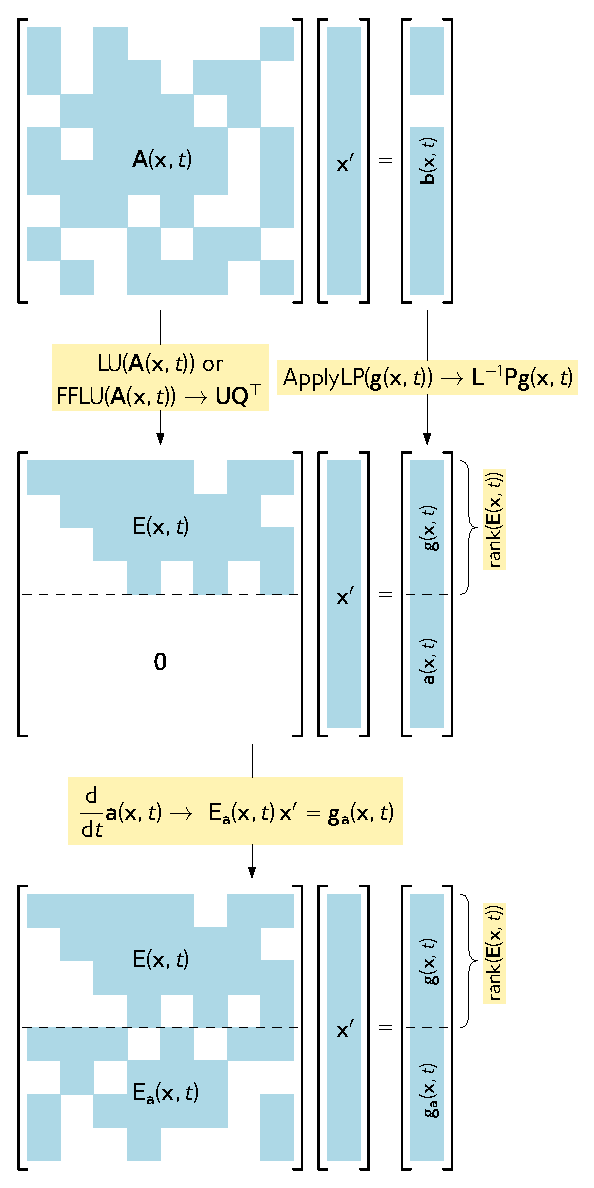
\includegraphics[width=1.0\textwidth, trim={0cm 7.35cm 0cm 0cm}, clip]{dae_visualization.eps}}
    \end{column}
  \end{columns}
\end{frame}

\subsubsection{Differentiation of Algebraic Equations}

\begin{frame}{Index Reduction Algorithm}{Differentiation of Algebraic Equations}
  \vspace{-1.0em}
  \begin{columns}
    \begin{column}[c]{0.6\textwidth}
      \begin{enumerate}[<+->]\setcounter{enumi}{2}
        \item \textbf{Differentiate} the algebraic equations $\ma$
        \begin{equation*}
          \dfrac{\text{d}}{\text{d}t} \ma = \mAd \mxp - \mgd
        \end{equation*}
        \item The new system of \acsp{DAE} takes the form
        \begin{align*}
          \mF = \mA &\mxp - \mb = \m{0} ~~ \text{with} \\
          \mA = \begin{bmatrix} \mE \\ \mAd \end{bmatrix}
          ~~ &\text{and} ~~
          \mb = \begin{bmatrix} \mg \\ \mgd \end{bmatrix}
        \end{align*}
        \item The differential index has been reduced by one!
      \end{enumerate}
      \uncover<4->{\begin{bbox}[A Sequential Algorithm]
        Apply \boxednumber{1}--\boxednumber{5} repeatedly until $\mA$ is non-singular.
      \end{bbox}}
    \end{column}
    \begin{column}[c]{0.4\textwidth}
      \visible<3->{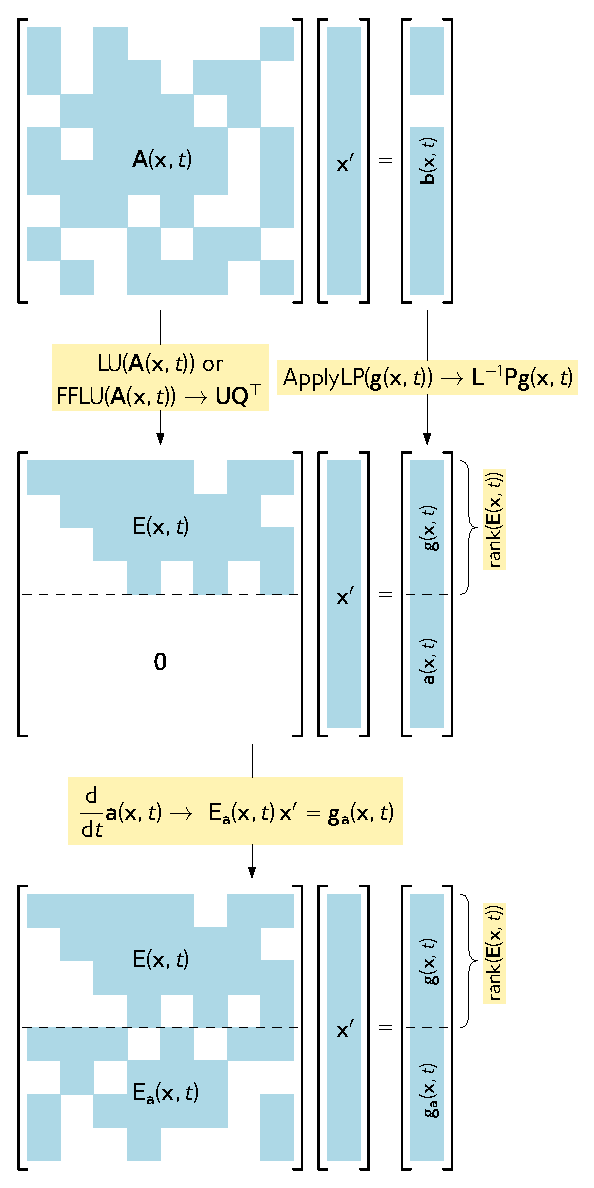
\includegraphics[width=1.0\textwidth, trim={0cm 0cm 0cm 7.35cm}, clip]{dae_visualization.eps}}
    \end{column}
  \end{columns}
\end{frame}

\begin{frame}{Index Reduction Algorithm}{Including Veiling Variables}
  \vspace{-1.0em}
  The algorithm can be extended to include \acs{LEM} \dots
  \begin{itemize}
    \item the veiling variables are stored in the list of $\mv$;
    \item the equations be also function of $\mv$;
    \item the veiling variables do just add an evaluation layer to the algorithm.
  \end{itemize}
  \visible<2->{\vspace{-1.5em}\hspace{-0.025\textwidth}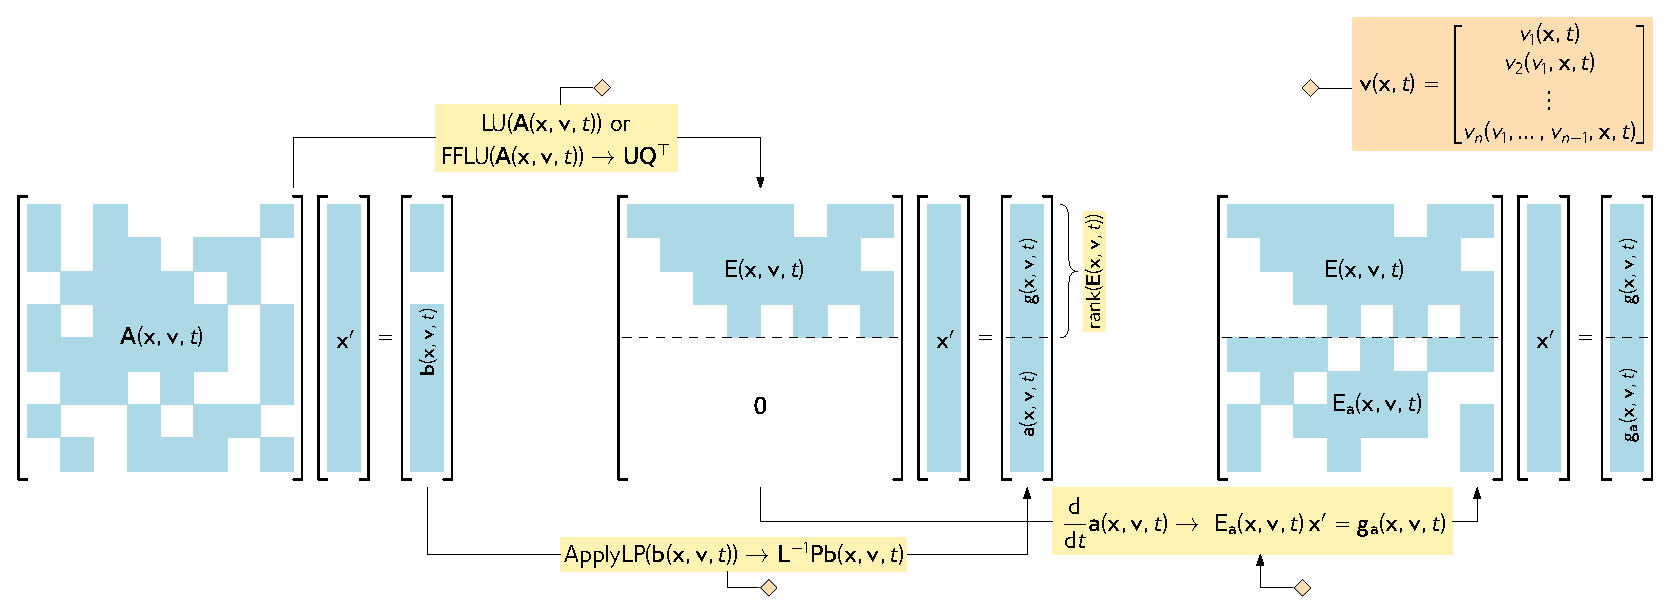
\includegraphics[width=1.05\textwidth]{dae_visualization_veil.eps}}
\end{frame}

\begin{frame}{Index Reduction Algorithm}{Algorithm Flowchart}
  \centering
  \begin{tikzpicture}[overlay]
    \node at (0,0) {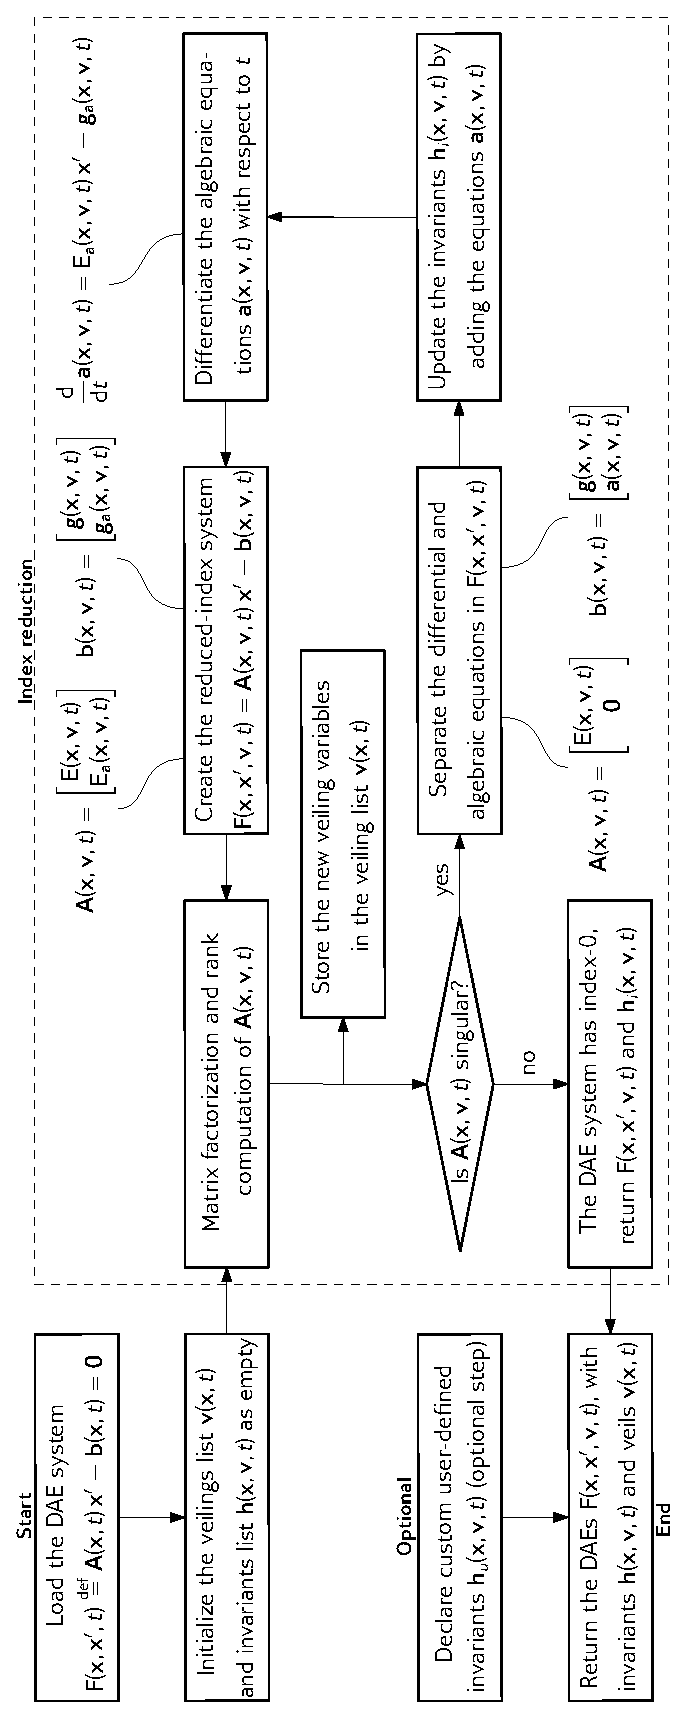
\includegraphics[angle=270, width=1.0\textwidth]{dae_flowchart_veil}};
    \only<1>{\draw[fg_sl_color, line width=1.0pt] (-7.2,  2.9) rectangle (-3.7,  0.4);} % Initialization
    \only<2>{\draw[fg_sl_color, line width=1.0pt] (-3.7,  2.9) rectangle ( 7.2, -2.9);} % Index Reduction
    \only<3>{\draw[fg_sl_color, dashed, line width=1.0pt] (-7.2, -0.3) rectangle (-3.7, -1.6);} % Optional step
    \only<4>{\draw[fg_sl_color, line width=1.0pt] (-7.2, -1.6) rectangle (-3.7, -2.9);} % Finalization
  \end{tikzpicture}
\end{frame}

\begin{frame}{Index Reduction Algorithm}{The Reduced \acs{DAE} System}
  The index-reduced system of \acsp{DAE} takes the form \dots
  \begin{itemize}[<+->]
    \item A \textbf{differential part}, which can be expressed as
    %
    \begin{equation*}
      \begin{array}{ccl}
          \m{F}(\mx, \mx^\prime, \m{v}, t) = \m{0} & \hspace{0.5cm} & \text{implicit  system class} \\
          \m{A}(\mx, \m{v}, t) \mx^\prime = \m{b}(\mx, \m{v}, t) & \hspace{0.5cm} & \text{semi-explicit system class} \\
          \mx^\prime = \m{f}(\mx, \m{v}, t) & \hspace{0.5cm} & \text{explicit system class}
      \end{array}
    \end{equation*}
    %
    \item The \textbf{invariants}, arising from the index reduction
    %
    \begin{equation*}
      \m{h}(\mx, \m{v}, t) = \begin{bmatrix}
          \mhiv \\
          \mhuv
      \end{bmatrix} = \m{0} \hspace{0.5cm} \begin{array}{l}
        \text{hidden constraints} \\
        \text{optional user-defined invariants}
    \end{array}
    \end{equation*}
    %
    \item The \textbf{veiling variables}, used to limit expression swell
    %
    \begin{equation*}
        \m{v}(\mx, t) = \begin{bmatrix}
            v_{1}(\mx, t) \\
            v_{2}(v_{1}, \mx, t) \\
            \vdots \\
            v_{n}(v_{1}, \dots, v_{n-1}, \mx, t)
        \end{bmatrix}
    \end{equation*}
  \end{itemize}
\end{frame}

\subsection{Projection on Invariants}

\begin{frame}{Projection on Invariants}{Theoretical Background and Implementation}
  \begin{columns}
    \begin{column}[c]{0.6\textwidth}
      Projection is performed \dots
      \begin{itemize}
        \item during the \textbf{numerical integration}
        \item to \textbf{enforce} the solution $\mx$ onto the $\mhv$ manifold
        \item by solving the \textbf{constrained minimization} problem
          \begin{align*}
            \underset{\mx}{\text{minimize}} \quad &\dfrac{1}{2}\left(\mx - \tilde{\mx}\right)^2 \\
            \text{subject to} \quad &\mhv = \m{0}
          \end{align*}
        \end{itemize}
      \end{column}
      \begin{column}[c]{0.4\textwidth}
        \hspace{-0.2\textwidth}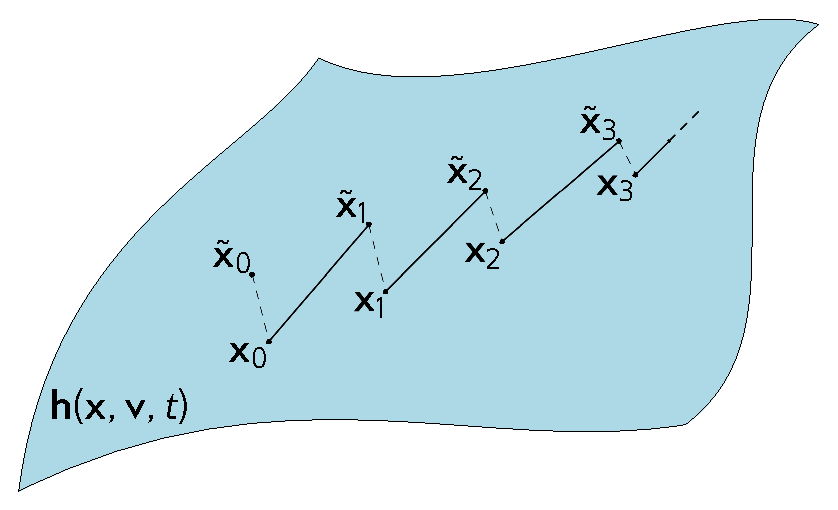
\includegraphics[width=1.2\textwidth]{projection.eps}
      \end{column}
    \end{columns}
    \vspace{1.0em}
    \hic{\large Find $\mx$ with minimal distance from $\tilde{\mx}$ that satisfies the invariants $\mhv$}
\end{frame}

\begin{frame}{Projection on Invariants}{Theoretical Background and Implementation}
  \begin{itemize}
    \item The \textbf{Lagrangian} of the minimization problem is
    \begin{equation*}
      \mathcal{L}(\mx, \boldsymbol{\lambda}) = \frac{1}{2}\left(\mx - \tilde{\mx}\right)^2 + \boldsymbol{\lambda} \cdot \mhv
      \quad \rightarrow \quad
      \begin{cases}
        \mx + \m{Jh}_\mx^\top \boldsymbol{\lambda} = \tilde{\mx} \\
        \mhv = \m{0}
      \end{cases}
    \end{equation*}
    \item The problem is solved using the iterative method
    \begin{equation*}
      \begin{bmatrix}
        \m{I}        & \m{Jh}_\mx^\top \\
        \m{Jh}_{\mx} & \m{0}
      \end{bmatrix}
      \begin{bmatrix}
        \delta\mx \\
        \boldsymbol{\lambda}
      \end{bmatrix} = \begin{bmatrix}
        \tilde{\mx} - \mx \\
        -\mhv
      \end{bmatrix} \quad \text{where the step is $\mx = \tilde{\mx} + \delta\mx$}
    \end{equation*}
    \item[] \dots derived from the \textbf{Taylor expansion}
    \begin{equation*}
      \begin{cases}
        \mhv + \m{Jh}_{\mx}(\mx, \m{v}, t) \delta\mx + \textcolor{mycolor2}{\mathcal{O}\left(\| \delta\mx \|^2\right)} = \m{0} \\
        \mx + \delta\mx + \m{Jh}_{\mx}^{\top}(\mx + \textcolor{mycolor2}{\delta \mx}, \m{v}, t) \boldsymbol{\lambda} = \tilde{\mx}
      \end{cases}
    \end{equation*}
  \end{itemize}
\end{frame}

\begin{frame}{Symbolic-Numerical Validation}{The Problem}
  \begin{columns}
    \begin{column}[t]{0.425\textwidth}
      A \textbf{particle} moving over a \textbf{torus} surface% on a \textbf{stable path}
      \begin{equation*}
        \label{chap4:eq:torus}
        \begin{cases}
          x^{\prime}_{1} = u_{1} \\
          x^{\prime}_{2} = u_{2} \\
          x^{\prime}_{3} = u_{3} \\
          u^{\prime}_{1} = u_{3}\cos(t) - x_{3}\sin(t) - u_{2} + 2 c x_{1}\lambda \\
          u^{\prime}_{2} = u_{3}\sin(t) + x_{3}\cos(t) + u_{1} + 2 c x_{2}\lambda \\
          u^{\prime}_{3} = x_{3} + 2x_{3}\lambda \\[-0.1em]
          \rho^2 = x_{1}^2 + x_{2}^2 + x_{3}^2 - 2r\sqrt{x_{1}^2 + x_{2}^2} + r^2
        \end{cases}
      \end{equation*}
      with $c = 1 - \dfrac{r}{\sqrt{x_{1}^2 + x_{2}^2}}$.
    \end{column}
    \begin{column}[t]{0.575\textwidth}
      \vspace{-3.0em}
      \hic{\large A stable path \dots}
      with $\mx_{0} = [15, 0, 0, 0, 15, -5, \lambda]^{\top}$ and parameters $\rho = 5$ and $r = 10$ is given by
      \begin{equation*}
        \mx_\text{exact} = \begin{bmatrix}
          x_{1} \\ x_{2} \\ x_{3}
        \end{bmatrix} = \begin{bmatrix}
          (\rho \cos(2\pi - t) + r) \cos(t) \\
          (\rho \cos(2\pi - t) + r) \sin(t) \\
          \rho \sin(2\pi - t)
        \end{bmatrix}
      \end{equation*} \\[-3.0em]
      \centering{
      %%  \begin{tikzpicture}
      %%    \begin{axis}[
      %%      xtick=\empty, ytick=\empty, ztick=\empty,
      %%      axis line style={draw=none},
      %%      tick style={draw=none},
      %%      axis equal,
      %%      view={100}{40}]
      %%      \addplot3[surf,
      %%        samples=50,
      %%        color=mycolor1, opacity=0.25,
      %%        faceted color=mycolor1!20,
      %%        domain=0:2*pi,
      %%        y domain=0:2*pi,
      %%        z buffer=sort]
      %%        ({(10+5*cos(deg(x)))*cos(deg(y+pi/2))},
      %%          {(10+5*cos(deg(x)))*sin(deg(y+pi/2))},
      %%          {5*sin(deg(x))});
      %%      \addplot3[variable=\t,
      %%        no markers,
      %%        samples=50,
      %%        color=mycolor4,
      %%        domain=0:2*pi,
      %%        line width=0.1pt, dashed]
      %%        ({(10+5*cos(deg(2*pi-\t)))*cos(deg(\t))},
      %%          {(10+5*cos(deg(2*pi-\t)))*sin(deg(\t))},
      %%          {5*sin(deg(2*pi-\t))});
      %%      \addplot3[
      %%        mark=*, mark size=1.0pt,
      %%        color=mycolor4]
      %%        ({(10+5*cos(deg(2*pi-0.1*pi)))*cos(deg(0.1*pi))},
      %%          {(10+5*cos(deg(2*pi-0.1*pi)))*sin(deg(0.1*pi))},
      %%          {5*sin(deg(2*pi-0.1*pi))});
      %%    \end{axis}
      %%\end{tikzpicture}
      %\animategraphics[
      %  controls, loop
      %]{12}{gif_generation/torus/torus_png/torus1-}{1}{3}
      }
    \end{column}
  \end{columns}
\end{frame}

\begin{frame}{Symbolic-Numerical Validation}{Order and Error Analysis}
  \vspace{-1.0em}
  \hic{The order and the invariants are preserved}
  \centering{\small{
\begin{tikzpicture}

\begin{axis}[%
  title={Runge-Kutta Methods Order},
  title style={yshift=0.0mm, font=\bfseries},
  minor tick num=1,
  minor grid style={dashed, line width=0.1pt, draw=gray!45},
  major grid style={line width=0.2pt, draw=gray!60},
  width=4.5cm,
  height=4.5cm,
  at={(0.0in,0.0in)},
  scale only axis,
  xmode=log,
  xmin=0.005,
  xmax=0.5,
  xminorticks=true,
  xlabel style={font=\color{black}},
  xlabel={$\Delta t$},
  ymode=log,
  ymin=5.0e-16,
  ymax=20.0,
  yminorticks=true,
  ylabel style={font=\color{black}},
  ylabel={$\varepsilon$},
  axis background/.style={fill=none},
  xmajorgrids,
  xminorgrids,
  ymajorgrids,
  yminorgrids,
  legend style={font=\small, at={(0.97,0.03)}, anchor=south east, legend cell align=left, align=left, draw=black}
]

\addplot[color=mycolor1, line width=0.5pt, mark=*, mark options={fill, scale=0.5, mycolor1}]
  table[row sep=crcr]{%
  0.005 1.879399452620709e-01\\
  0.06 1.711573027753681e+00\\
  0.115 3.063916890081130e+00\\
  0.17 4.231237958056623e+00\\
  0.225 6.302317678343108e+00\\
  0.28 8.762767335676816e+00\\
  0.335 1.028329978855519e+01\\
  0.39 1.252649980402613e+01\\
  0.445 9.207336428245306e+00\\
  0.5 1.299428017259284e+01\\
};
\addlegendentry{Implicit Euler}

\addplot[color=mycolor2, line width=0.5pt, mark=*, mark options={fill, scale=0.5, mycolor2}]
  table[row sep=crcr]{%
  0.005 1.992528035899e-07\\
  0.06 0.000337631444430997\\
  0.115 0.00233186668661123\\
  0.17 0.00737183144006526\\
  0.225 0.0166514146938725\\
  0.28 0.0314018007261607\\
  0.335 0.0510617453643611\\
  0.39 0.0786646899717534\\
  0.445 0.11675270797915\\
  0.5 0.170354895882445\\
};
\addlegendentry{RadauIIA3}

\addplot[color=mycolor4, line width=0.5pt, mark=*, mark options={fill, scale=0.5, mycolor4}]
  table[row sep=crcr]{%
  0.005 6.75015598972095e-14\\
  0.06 1.52360311034272e-08\\
  0.115 3.82347098870639e-07\\
  0.17 2.62977937026676e-06\\
  0.225 1.20705485162631e-05\\
  0.28 3.98898559916816e-05\\
  0.335 0.000112061177007128\\
  0.39 0.000269397467860699\\
  0.445 0.000580087484554959\\
  0.5 0.00113800574884237\\
};
\addlegendentry{RadauIIA5}

\addplot[area legend, draw=none, fill=mycolor1, fill opacity=0.5, forget plot]
  table[row sep=crcr] {%
  x y\\
  0.005 0.187939945262071\\
  0.015 0.187939945262071\\
  0.015 0.494964142080998\\
}--cycle;

\addplot[area legend, draw=none, fill=mycolor2, fill opacity=0.5, forget plot]
  table[row sep=crcr] {%
  x y\\
  0.005 1.992528035899e-07\\
  0.015 1.992528035899e-07\\
  0.015 5.45505603722094e-06\\
}--cycle;

\addplot[area legend, draw=none, fill=mycolor4, fill opacity=0.5, forget plot]
  table[row sep=crcr] {%
  x y\\
  0.005 6.75015598972095e-14\\
  0.015 6.75015598972095e-14\\
  0.015 1.57024270189941e-11\\
}--cycle;

\node[draw, fill=white] at (1.05e-2, 2.00e-02) {\footnotesize{$p = 0.932$}};
\node[draw, fill=white] at (1.05e-2, 2.10e-08) {\footnotesize{$p = 2.958$}};
\node[draw, fill=white] at (1.05e-2, 0.65e-14) {\footnotesize{$p = 5.095$}};
\end{axis}

\begin{axis}[%
  title={Projection Error},
  title style={yshift=0.0mm, font=\bfseries},
  minor tick num=1,
  minor grid style={dashed, line width=0.1pt, draw=gray!45},
  major grid style={line width=0.2pt, draw=gray!60},
  width=4.5cm,
  height=4.5cm,
  at={(7.0cm,0.0in)},
  scale only axis,
  xmin=0,
  xmax=6.28318530717959,
  xlabel style={font=\color{black}},
  xlabel={$t$},
  xlabel shift={0.125em},
  xtick={0, 1.5707963267949, 3.14159265358979, 4.71238898038469, 6.28318530717959},
  xticklabels={$0$, $\pi/2$, $\pi$, $3\pi/2$, $2\pi$},
  %every y tick scale label/.style={
  %  at={(1.015, 0.945)}, anchor=south west, inner sep=0pt
  %},
  ytick scale label code/.code={$\times \, 10^{-13}$},
  ymin=-0.02e-13,
  ymax=1.085e-13,
  ylabel style={font=\color{black}},
  ylabel={$\| \mh \|_{\infty}$},
  %yticklabel pos=right,
  axis background/.style={fill=none},
  xmajorgrids,
  xminorgrids,
  ymajorgrids,
  yminorgrids,
  legend style={font=\small, at={(0.5,0.97)}, anchor=north, legend cell align=left, align=left, draw=black}
]

\addplot[color=mycolor1, line width=0.5pt]
  table[row sep=crcr]{%
  0.0	0\\
  0.06	4.34990500158268e-14\\
  0.12	9.14713630327889e-14\\
  0.18	2.98902106951307e-14\\
  0.24	1.07748232567088e-13\\
  0.3	2.10810383283768e-14\\
  0.36	0\\
  0.42	4.71502785877585e-15\\
  0.48	3.60007915114583e-14\\
  0.54	5.15958404494974e-14\\
  0.6	0\\
  0.66	3.37571546641056e-14\\
  0.72	3.20051218006002e-14\\
  0.78	3.81173776267159e-14\\
  0.84	6.1954391364817e-15\\
  0.9	8.95925122577517e-14\\
  0.96	0\\
  1.02	0\\
  1.08	3.24241260150387e-14\\
  1.14	3.14931663864555e-14\\
  1.2	2.50556225451883e-14\\
  1.26	5.09349295084449e-15\\
  1.32	0\\
  1.38	2.64245779923981e-15\\
  1.44	3.6842072004579e-14\\
  1.5	5.61897690710851e-15\\
  1.56	0\\
  1.62	4.8026106429562e-14\\
  1.68	3.63626524685878e-14\\
  1.74	1.01942880461704e-14\\
  1.8	0\\
  1.86	1.60069355130316e-14\\
  1.92	2.28518820214578e-16\\
  1.98	1.59079989935601e-14\\
  2.04	0\\
  2.1	1.27449819572632e-15\\
  2.16	0\\
  2.22	1.5182461883964e-14\\
  2.28	0\\
  2.34	2.15531930059804e-14\\
  2.4	4.76121391456162e-15\\
  2.46	9.36392103102618e-15\\
  2.52	1.68888906404432e-14\\
  2.58	1.40704033684351e-14\\
  2.64	1.86604175798768e-14\\
  2.7	0\\
  2.76	1.9584060661875e-14\\
  2.82	0\\
  2.88	1.59393949940154e-14\\
  2.94	9.17721100927432e-15\\
  3	7.80968852312227e-15\\
  3.06	7.388064091316e-15\\
  3.12	7.28584971153018e-15\\
  3.18	1.58906318290303e-14\\
  3.24	8.71670113035874e-15\\
  3.3	2.01335164715821e-14\\
  3.36	1.87429669449795e-14\\
  3.42	1.7813725413259e-14\\
  3.48	1.60851063568547e-14\\
  3.54	6.25687551665572e-16\\
  3.6	1.69547170411231e-14\\
  3.66	8.41775766141766e-15\\
  3.72	3.39216511899456e-14\\
  3.78	4.45866709099199e-15\\
  3.84	1.91680683420683e-14\\
  3.9	2.35877773802524e-14\\
  3.96	4.31470535972855e-14\\
  4.02	3.27790567623137e-14\\
  4.08	3.33643422441018e-14\\
  4.14	8.33060192023164e-15\\
  4.2	0\\
  4.26	2.99541085364436e-14\\
  4.32	1.53853495359176e-14\\
  4.38	0\\
  4.44	0\\
  4.5	0\\
  4.56	4.11555718048816e-15\\
  4.62	3.67780794600896e-14\\
  4.68	6.96692544670932e-15\\
  4.74	3.21649541394723e-15\\
  4.8	0\\
  4.86	1.98207634010965e-14\\
  4.92	0\\
  4.98	3.98983227546346e-14\\
  5.04	2.66738145006334e-15\\
  5.1	0\\
  5.16	1.14818597398386e-15\\
  5.22	2.94481485016782e-14\\
  5.28	4.00430584084634e-14\\
  5.34	8.39165155939648e-16\\
  5.4	2.62190029363372e-14\\
  5.46	0\\
  5.52	4.5388851313787e-14\\
  5.58	0\\
  5.64	2.69606312402563e-15\\
  5.7	1.82222934912061e-14\\
  5.76	1.89070359423442e-14\\
  5.82	4.45295027597655e-14\\
  5.88	3.65018441462149e-14\\
  5.94	1.76619003298675e-14\\
  6	4.4664737416553e-14\\
  6.06	3.00820691761593e-14\\
  6.12	4.79911837055461e-14\\
  6.18	1.29969770362389e-14\\
  6.24	8.14452283860879e-14\\
};\addlegendentry{Implicit Euler}

\addplot[color=mycolor2, line width=0.5pt]
  table[row sep=crcr]{%
  0	0\\
  0.06	8.84448873691838e-15\\
  0.12	7.10252993448526e-14\\
  0.18	2.73745627106684e-14\\
  0.24	7.98778880425246e-14\\
  0.3	3.6081075739454e-14\\
  0.36	0\\
  0.42	3.24265476848927e-14\\
  0.48	3.87046037491941e-14\\
  0.54	6.15239311809982e-14\\
  0.6	0\\
  0.66	3.91562582690368e-14\\
  0.72	2.25000036079271e-14\\
  0.78	4.04414271599053e-14\\
  0.84	1.49380061235967e-14\\
  0.9	5.89354034123046e-14\\
  0.96	4.43960827492856e-14\\
  1.02	3.38273659792399e-14\\
  1.08	0\\
  1.14	1.23582540282663e-14\\
  1.2	1.54714760360776e-14\\
  1.26	4.93042497956856e-14\\
  1.32	9.19872936629242e-15\\
  1.38	1.38615479184773e-15\\
  1.44	7.52495018973183e-16\\
  1.5	4.80001254407006e-14\\
  1.56	1.82980829289806e-14\\
  1.62	4.90034281627552e-16\\
  1.68	3.13259870821234e-14\\
  1.74	1.77625688404132e-14\\
  1.8	3.02811591570971e-14\\
  1.86	1.85416404827173e-14\\
  1.92	6.38757726249384e-15\\
  1.98	1.0616430615281e-14\\
  2.04	2.86913740347028e-14\\
  2.1	2.87532747854972e-14\\
  2.16	1.44908645537467e-14\\
  2.22	0\\
  2.28	1.48226453812946e-14\\
  2.34	1.6245848597906e-14\\
  2.4	3.22231789091681e-14\\
  2.46	2.92696331143997e-14\\
  2.52	1.74008700537511e-14\\
  2.58	1.77789685566004e-14\\
  2.64	1.44343986204923e-14\\
  2.7	0\\
  2.76	0\\
  2.82	6.40702877095534e-15\\
  2.88	1.42771571465927e-14\\
  2.94	2.0554256596902e-14\\
  3	7.06195117559697e-15\\
  3.06	0\\
  3.12	7.27089394097636e-15\\
  3.18	4.06350200553687e-14\\
  3.24	3.53559108943528e-16\\
  3.3	1.59074571212465e-14\\
  3.36	6.78088594942458e-15\\
  3.42	0\\
  3.48	0\\
  3.54	6.37313833585726e-15\\
  3.6	2.64233294813674e-14\\
  3.66	9.05705974224811e-15\\
  3.72	9.25806216032326e-15\\
  3.78	2.8421709430404e-14\\
  3.84	0\\
  3.9	3.29455139897558e-14\\
  3.96	1.07330281365035e-14\\
  4.02	0\\
  4.08	2.99993820655985e-14\\
  4.14	2.99302413301819e-14\\
  4.2	8.45649099423198e-15\\
  4.26	0\\
  4.32	2.92414129726747e-14\\
  4.38	1.55071468737394e-14\\
  4.44	2.89702385935865e-14\\
  4.5	3.11590712535806e-14\\
  4.56	8.06643782767062e-15\\
  4.62	3.71860560727394e-14\\
  4.68	1.15774417663157e-14\\
  4.74	2.40000466840985e-15\\
  4.8	7.99747337593166e-16\\
  4.86	2.49901770525562e-14\\
  4.92	6.77554661163664e-15\\
  4.98	1.2538207925704e-14\\
  5.04	3.03245905494408e-14\\
  5.1	2.16408472173715e-15\\
  5.16	1.40062502346563e-14\\
  5.22	3.81524411539504e-14\\
  5.28	3.8071688841407e-14\\
  5.34	1.57202927985259e-14\\
  5.4	3.0377210200149e-14\\
  5.46	7.15590051863223e-14\\
  5.52	4.38239782516872e-14\\
  5.58	1.79951982640777e-14\\
  5.64	6.39867062902223e-14\\
  5.7	6.49615736545083e-14\\
  5.76	1.66177595708798e-14\\
  5.82	1.07695444051526e-13\\
  5.88	0\\
  5.94	3.46718274762021e-14\\
  6	6.08947400862772e-14\\
  6.06	6.27262279676494e-14\\
  6.12	1.05156307287711e-13\\
  6.18	5.75007020364114e-14\\
  6.24	1.72627172653053e-14\\
};
\addlegendentry{RadauIIA3}

\addplot[color=mycolor4, line width=0.5pt]
  table[row sep=crcr]{%
  0	0\\
  0.06	6.71403541230021e-14\\
  0.12	3.77283965133535e-14\\
  0.18	6.34330992622269e-14\\
  0.24	0\\
  0.3	4.65706896752599e-14\\
  0.36	3.53024518099557e-14\\
  0.42	0\\
  0.48	6.01556977798936e-14\\
  0.54	5.6843418860808e-14\\
  0.6	6.3998447010507e-14\\
  0.66	6.89462466735111e-14\\
  0.72	1.11734380999568e-14\\
  0.78	5.84336673739155e-15\\
  0.84	4.51547342643318e-14\\
  0.9	2.40345531292498e-14\\
  0.96	1.35285891842221e-14\\
  1.02	4.89969933702126e-14\\
  1.08	6.44519721994705e-14\\
  1.14	3.82027084757365e-14\\
  1.2	4.63610229041449e-14\\
  1.26	2.14012786085607e-14\\
  1.32	3.62129381964501e-14\\
  1.38	5.14278476238434e-14\\
  1.44	7.52475217963951e-16\\
  1.5	1.51595717211594e-14\\
  1.56	2.01357850117944e-15\\
  1.62	4.90016969470829e-16\\
  1.68	2.15197114109576e-15\\
  1.74	1.42094637215295e-14\\
  1.8	9.14135367252492e-15\\
  1.86	0\\
  1.92	3.33136607299302e-14\\
  1.98	3.83629683826335e-14\\
  2.04	1.59967695360947e-14\\
  2.1	2.94212446823591e-14\\
  2.16	0\\
  2.22	1.51864101443109e-14\\
  2.28	7.27563915445106e-15\\
  2.34	1.93360441784085e-14\\
  2.4	0\\
  2.46	2.9511735315762e-14\\
  2.52	0\\
  2.58	1.77786569080783e-14\\
  2.64	2.85341341331248e-14\\
  2.7	3.06062249475849e-14\\
  2.76	6.05430255954215e-15\\
  2.82	1.35178386471263e-15\\
  2.88	0\\
  2.94	0\\
  3	0\\
  3.06	3.54093358009643e-16\\
  3.12	1.42133513334771e-14\\
  3.18	1.77504779217282e-16\\
  3.24	7.24938179967691e-15\\
  3.3	7.00937076054701e-15\\
  3.36	2.84301825312368e-14\\
  3.42	6.63882013161966e-15\\
  3.48	1.6007712487894e-14\\
  3.54	1.62299374575982e-14\\
  3.6	0\\
  3.66	1.58874434059998e-14\\
  3.72	1.44195741501297e-14\\
  3.78	9.49801118770299e-15\\
  3.84	1.49386437805692e-14\\
  3.9	0\\
  3.96	7.70015247254448e-15\\
  4.02	1.15286998476027e-14\\
  4.08	1.04060301103914e-14\\
  4.14	2.10957320580662e-14\\
  4.2	5.76430753406985e-14\\
  4.26	0\\
  4.32	3.43798720861495e-15\\
  4.38	0\\
  4.44	0\\
  4.5	1.29595646328969e-14\\
  4.56	2.84138752512645e-14\\
  4.62	4.71567077252452e-15\\
  4.68	3.33738140247112e-14\\
  4.74	2.02937095842527e-14\\
  4.8	1.53930076582013e-14\\
  4.86	7.91332496467288e-15\\
  4.92	4.76635995797504e-14\\
  4.98	4.81895564192324e-14\\
  5.04	1.16266826302188e-14\\
  5.1	6.2319428928642e-14\\
  5.16	4.3455302159109e-14\\
  5.22	2.86730496772646e-14\\
  5.28	2.9300964947864e-14\\
  5.34	6.72223560445336e-15\\
  5.4	7.0170982385832e-14\\
  5.46	4.40352521641556e-14\\
  5.52	8.35122710587472e-15\\
  5.58	2.20814842274086e-14\\
  5.64	5.55417576536816e-14\\
  5.7	2.55536510002858e-14\\
  5.76	2.1865754534927e-14\\
  5.82	8.783763173108e-14\\
  5.88	7.96680804218409e-14\\
  5.94	6.22830583836424e-14\\
  6	1.18139987543405e-14\\
  6.06	1.67364446109691e-14\\
  6.12	3.86667246627752e-14\\
  6.18	3.79629193314912e-15\\
  6.24	6.70788729037476e-14\\
};
\addlegendentry{RadauIIA5}

\end{axis}

\end{tikzpicture}%}}
\end{frame}

\begin{frame}{Symbolic-Numerical Validation}{Solution Visualization}
  \begin{minipage}[c]{0.22\textwidth}
    \hic{\large The importance of projection \dots}
    $\Delta t = 0.025$\,s \\ $t \in [0, 400\pi]$\,s
  \end{minipage}
  \begin{minipage}[c]{0.77\textwidth}
    \vspace{-2.0em}
    \small{\begin{tikzpicture}

\begin{axis}[%
  minor tick num=1,
  minor grid style={dashed, line width=0.1pt, draw=gray!45},
  major grid style={line width=0.2pt, draw=gray!60},
  width=4.0cm,
  height=4.0cm,
  at={(0.0in, 0.0in)},
  scale only axis,
  xmin=-17.5,
  xmax=17.5,
  xlabel style={font=\color{black}},
  xlabel={$x_1$},
  ymin=-17.5,
  ymax=17.5,
  ylabel style={font=\color{black}},
  ylabel={$x_2$},
  ylabel shift={-0.5em},
  axis background/.style={fill=none},
  xmajorgrids,
  xminorgrids,
  ymajorgrids,
  yminorgrids
]

\fill[mycolor1, opacity=0.3, even odd rule] (0,0) circle[radius=15] circle[radius=5];

\addplot[color=mycolor4, opacity=1.0, line width=0.5pt, forget plot]
  table[row sep=crcr]{%
  15	0\\
  14.9937508137425	0.374921882323731\\
  14.9750130171408	0.749375234323529\\
  14.9438158759563	1.12289240391071\\
  14.9002080973756	1.49500749345469\\
  14.8442577265697	1.86525723198851\\
  14.7760520021723	2.23318184138845\\
  14.6956971711638	2.59832589457273\\
  14.6033182634139	2.96023916371928\\
  14.4990588265636	3.31847745659132\\
  14.3830806218317	3.6726034390532\\
  14.2555632814289	4.02218744188373\\
  14.1167039285264	4.36680825009529\\
  13.9667167605155	4.70605387290265\\
  13.8058325966784	5.03952229263938\\
  13.6342983913069	5.3668221909113\\
  13.4523767133948	5.68757365032568\\
  13.2603451942497	6.00140883027312\\
  13.0584959441994	6.30797261516682\\
  12.8471349398866	6.60692323374637\\
  12.6265813835739	6.89793284804678\\
  12.397167035958	7.18068811070543\\
  12.1592355241578	7.45489068943992\\
  11.9131416264155	7.72025775746472\\
  11.6592505352869	7.97652244884259\\
  11.3979371010423	8.22343427776877\\
  11.1295850570541	8.46075952087566\\
  10.8545862290595	8.68828156181298\\
  10.5733397300985	8.90580119731441\\
  10.2862511430837	9.11313690419081\\
  9.99373169291373	9.31012506670692\\
  9.69619741007433	9.49662016389985\\
  9.39406828772691	9.6724949165564\\
  9.08776743423141	9.83764039355499\\
  8.77772022312239	9.99196607748552\\
  8.46435344252308	10.1353998894956\\
  8.14809444598937	10.2678881734179\\
  7.82937030677734	10.3893956393711\\
  7.5086069774998	10.4999052670542\\
  7.18622845713732	10.5994181691215\\
  6.86265596733788	10.6879534150805\\
  6.53830713991898	10.7655478162592\\
  6.21359521744759	10.8322556724947\\
  5.88892826875022	10.8881484812641\\
  5.56470842115362	10.9333146100911\\
  5.24133111121871	10.9678589331361\\
  4.91918435568441	10.9919024329704\\
  4.5986480442715	11.005581768609\\
  4.28009325596341	11.0090488109701\\
  3.96388160029658	11.0024701469934\\
  3.65036458514248	10.9860265537317\\
  3.33988301239428	10.9599124438032\\
  3.03276640288896	10.9243352836395\\
  2.72933245184042	10.8795149860648\\
  2.42988651596175	10.8256832787627\\
  2.13472113338716	10.7630830502736\\
  1.84411557741373	10.6919676751855\\
  1.55833544500332	10.6126003202706\\
  1.27763228089195	10.5252532333212\\
  1.00224323806637	10.4302070165104\\
  0.732390775277458	10.3277498861021\\
  0.468282392162512	10.2181769204107\\
  0.210110402458937	10.10178929789\\
  -0.0419482543094117	9.97889352728501\\
  -0.287732162379363	9.84980067176283\\
  -0.527095540345793	9.71482556899192\\
  -0.75990831270954	9.57428604910142\\
  -0.986056142385723	9.42850215248531\\
  -1.20544042426526	9.27779534938354\\
  -1.41797824003955	9.12248776319712\\
  -1.62360227457437	8.96290139944722\\
  -1.82226069423124	8.79935738229363\\
  -2.01391698761099	8.63217520048434\\
  -2.19854976931135	8.46167196460351\\
  -2.37615254735818	8.28816167742946\\
  -2.54673345507844	8.11195451919342\\
  -2.71031494825183	7.93335614947457\\
  -2.86693346848844	7.75266702743668\\
  -3.01663907383792	7.57018175204608\\
  -3.15949503773575	7.38618842386731\\
  -3.29557741745072	7.20096802996551\\
  -3.42497459329632	7.01479385339318\\
  -3.54778677991655	6.82793090866284\\
  -3.66412551104272	6.64063540454585\\
  -3.77411309916434	6.45315423545738\\
  -3.87788207164088	6.26572450262211\\
  -3.97557458481495	6.07857306612654\\
  -4.06734181775832	5.89191612889098\\
  -4.15334334731205	5.70595885350067\\
  -4.23374650615094	5.52089501276336\\
  -4.30872572561758	5.33690667475803\\
  -4.37846186512711	5.15416392306235\\
  -4.44314152995201	4.97282461273883\\
  -4.50295637925287	4.79303416258877\\
  -4.55810242621197	4.61492538406632\\
  -4.60877933216882	4.43861834716921\\
  -4.65518969663866	4.2642202835036\\
  -4.69753834514373	4.0918255266562\\
  -4.73603161674677	3.92151548987803\\
  -4.77087665320955	3.75335868101424\\
  -4.80228069164967	3.58741075448838\\
  -4.83045036261457	3.42371460009418\\
  -4.85559099541549	3.26230046821244\\
  -4.87790593259225	3.10318613100918\\
  -4.897595855295	2.94637707904345\\
  -4.91485812141753	2.79186675266909\\
  -4.92988611820044	2.63963680747764\\
  -4.94286863104935	2.48965741297949\\
  -4.95398923019248	2.34188758359673\\
  -4.96342567685692	2.19627554100771\\
  -4.9713493504853	2.05275910675323\\
  -4.97792469854355	1.91126612397451\\
  -4.98330871031458	1.77171490704179\\
  -4.98765041613668	1.63401471780707\\
  -4.99109041334799	1.49806626710029\\
  -4.99376042023238	1.36376224005774\\
  -4.99578285907381	1.2309878437795\\
  -4.99727046950046	1.09962137579335\\
  -4.99832595306767	0.969534811711893\\
  -4.99904165006738	0.840594410447134\\
  -4.99949924933887	0.712661335280924\\
  -4.99976953193715	0.585592289072316\\
  -4.99991214925682	0.4592401618245\\
  -4.99997543625228	0.33345468881619\\
  -4.9999962601649	0.208083117468957\\
  -4.9999999052545	0.0829708811035305\\
  -4.99999999375738	-0.0420377222823968\\
  -4.99999844333905	-0.167098848096572\\
  -4.99998546107185	-0.292368421974906\\
  -4.99993957405531	-0.418001457244979\\
  -4.99982769651727	-0.544151374910845\\
  -4.99960523328002	-0.670969328051114\\
  -4.99921621924076	-0.798603532484824\\
  -4.9985934945988	-0.927198605581879\\
  -4.99765891529097	-1.0568949150346\\
  -4.99632359813945	-1.18782793941524\\
  -4.9944881999953	-1.32012764227316\\
  -4.99204323023475	-1.45391786154742\\
  -4.98886939571552	-1.58931571597376\\
  -4.9848379773367	-1.72643103016838\\
  -4.97981123714917	-1.86536577997099\\
  -4.97364285502352	-2.00621355964768\\
  -4.96617839366465	-2.14905907242748\\
  -4.95725579079108	-2.2939776458429\\
  -4.9467058771312	-2.44103477322221\\
  -4.93435291893412	-2.59028568269127\\
  -4.92001518351491	-2.74177493489499\\
  -4.90350552637446	-2.89553605063471\\
  -4.88463199830537	-3.05159116948109\\
  -4.86319847092599	-3.2099507404196\\
  -4.83900527895141	-3.37061324542646\\
  -4.81184987752423	-3.53356495684698\\
  -4.7815275128381	-3.69877972930553\\
  -4.74783190430539	-3.86621882685731\\
  -4.71055593643394	-4.03583078593238\\
  -4.66949235858719	-4.20755131458162\\
  -4.62443449075155	-4.38130322839449\\
  -4.57517693344536	-4.55699642342037\\
  -4.52151627986221	-4.73452788627421\\
  -4.46325182835038	-4.9137817415515\\
  -4.40018629331614	-5.09462933654776\\
  -4.33212651264738	-5.27692936322004\\
  -4.25888414975254	-5.46052801719404\\
  -4.1802763883233	-5.64525919355004\\
  -4.09612661794674	-5.83094471900767\\
  -4.00626510870719	-6.01739462005352\\
  -3.91052967294857	-6.20440742644464\\
  -3.80876631239165	-6.39177050943945\\
  -3.70082984884335	-6.57926045401352\\
  -3.58658453676064	-6.76664346422931\\
  -3.46590465598776	-6.95367580084273\\
  -3.33867508302252	-7.14010425014199\\
  -3.20479183922895	-7.32566662294101\\
  -3.06416261445601	-7.51009228255518\\
  -2.91670726459435	-7.69310270052672\\
  -2.76235828165738	-7.87441203877909\\
  -2.60106123504679	-8.0537277568277\\
  -2.43277518272452	-8.23075124258217\\
  -2.25747305109535	-8.40517846523755\\
  -2.07514198247518	-8.57670064867195\\
  -1.88578364910264	-8.74500496373433\\
  -1.68941453273234	-8.90977523772561\\
  -1.48606616893359	-9.070692679358\\
  -1.27578535530688	-9.22743661741181\\
  -1.05863432291518	-9.37968525129208\\
  -0.834690870325286	-9.52711641162571\\
  -0.604048459739985	-9.66940832903726\\
  -0.366816274802283	-9.80624040919673\\
  -0.123119239739772	-9.9372940122296\\
  0.126902000374298	-10.0622532345434\\
  0.38309113838236	-10.1808056911348\\
  0.645276302857649	-10.2926432964201\\
  0.9132701949187	-10.3974630416448\\
  1.18687026387527	-10.4949677669158\\
  1.46585892145666	-10.5848669259242\\
  1.75000379426408	-10.6668773414295\\
  2.0390580140053	-10.7407239496017\\
  2.33276054495897	-10.8061405313356\\
  2.63083654803798	-10.8628704286823\\
  2.93299778071735	-10.910667244577\\
  3.23894303201237	-10.949295524076\\
  3.54835859159077	-10.9785314153601\\
  3.86091875202964	-10.9981633088063\\
  4.17628634313366	-11.0079924524822\\
  4.4941132971593	-11.0078335424685\\
  4.81404124369902	-10.9975152864773\\
  5.13570213291553	-10.9768809392941\\
  5.45871888573713	-10.9457888086382\\
  5.78270606955483	-10.9041127301038\\
  6.10727059790681	-10.8517425099251\\
  6.43201245255593	-10.7885843343715\\
  6.75652542632576	-10.714561144671\\
  7.08039788499711	-10.6296129764358\\
  7.40321354651444	-10.5336972626456\\
  7.72455227572283	-10.4267890993484\\
  8.0439908927865	-10.3088814732971\\
  8.36110399343142	-10.1799854508634\\
  8.67546477910684	-10.0401303276462\\
  8.98664589512859	-9.88936373827947\\
  9.29422027487393	-9.72775172607745\\
  9.59776198802864	-9.5553787721906\\
  9.89684709092526	-9.37234778410336\\
  10.1910544769745	-9.1787800433703\\
  10.4799667251816	-8.97481511258001\\
  10.7631709447914	-8.76061070168478\\
  11.0402596140261	-8.53634249384668\\
  11.3108314109759	-8.30220393113459\\
  11.5744920346737	-8.05840596045557\\
  11.8308550143938	-7.80517674019692\\
  12.0795425053195	-7.54276130821033\\
  12.320186068621	-7.27142121175998\\
  12.5524274341534	-6.99143410025238\\
  12.7759192439511	-6.70309328159722\\
  12.9903257747238	-6.40670724313605\\
  13.1953236377247	-6.10259913822372\\
  13.3906024542157	-5.79110623952327\\
  13.5758655050099	-5.47257936026373\\
  13.7508303525172	-5.14738224472656\\
  13.9152294337799	-4.81589092930378\\
  14.0688106231894	-4.47849307559688\\
  14.2113377634044	-4.13558727699824\\
  14.3425911633112	-3.78758234035687\\
  14.4623680618042	-3.43489654433605\\
  14.5704830562381	-3.07795687613228\\
  14.6667684946576	-2.71719824831625\\
  14.7510748306964	-2.35306269753697\\
  14.8232709404292	-1.98599856694236\\
  14.8832444003762	-1.6164596741694\\
  14.9309017259495	-1.24490446680053\\
  14.9661685699131	-0.871795167227203\\
  14.9889898801943	-0.497596908861645\\
  14.9993300168099	-0.122776865684432\\
  14.9971728275823	0.252196622883704\\
  14.982521682415	0.626854929777078\\
  14.9553994661915	1.00073001874566\\
  14.9158485301205	1.37335532145559\\
  14.8639306017886	1.74426661123003\\
  14.7997266540876	2.11300287142721\\
  14.7233367332822	2.47910715645627\\
  14.6348797467692	2.84212744349115\\
  14.534493210849	3.20161747289467\\
  14.4223329592501	3.55713757546355\\
  14.2985728130567	3.90825548459761\\
  14.1634042127852	4.25454713152544\\
  14.0170358136136	4.59559742182497\\
  13.8596930445621	4.93100099141115\\
  13.6916176328014	5.26036294032543\\
  13.5130670941801	5.58329954265186\\
  13.3243141911524	5.89943893093847\\
  13.1256463594994	6.20842175364385\\
  12.9173651050743	6.50990180405695\\
  12.6997853721075	6.80354661934549\\
  12.4732348845401	7.08903804838254\\
  12.2380534619275	7.36607278707568\\
  11.9945923116144	7.63436288008502\\
  11.7432132987616	7.89363618775372\\
  11.4842881960314	8.14363681730386\\
  11.2181979146847	8.38412551735453\\
  10.9453317188958	8.61488003491047\\
  10.666086425195	8.83569543413683\\
  10.3808655888657	9.04638437619494\\
  10.0900786792675	9.24677735964216\\
  9.79414024601509	9.43672292091727\\
  9.49346907796902	9.61608779453588\\
  9.18848735704562	9.78475703277657\\
  8.87961980880209	9.9426340846323\\
  8.56729285181554	10.0896408340049\\
  8.25193374784114	10.2257175971577\\
  7.93396975473805	10.3508230795487\\
  7.61382728414724	10.4649342922995\\
  7.29193106587917	10.5680464285892\\
  6.96870332096081	10.6601727004225\\
  6.64456294526005	10.7413441362794\\
  6.31992470558146	10.8116093402557\\
  5.99519845008435	10.8710342134091\\
  5.67078833485104	10.9197016380912\\
  5.34709206837487	10.9577111261593\\
  5.02450017569947	10.9851784320339\\
  4.70339528389045	11.0022351316572\\
  4.38415143045205	11.0090281684821\\
  4.06713339626547	11.0057193677128\\
  3.75269606453827	10.9924849200787\\
};
\end{axis}

\begin{axis}[%
  title={RadauIIA5 -- With projection},
  title style={yshift=-2.0mm, font=\bfseries},
  minor tick num=1,
  minor grid style={dashed, line width=0.1pt, draw=gray!45},
  major grid style={line width=0.2pt, draw=gray!60},
  width=4.0cm,
  height=2.0cm,
  at={(0.0in, 4.25cm)},
  scale only axis,
  xmin=-17.5,
  xmax=17.5,
  xlabel style={font=\color{black}},
  xlabel=\empty,
  xticklabels=\empty,
  ymin=-7.5,
  ymax=7.5,
  ylabel style={font=\color{black}},
  ylabel={$x_3$},
  axis background/.style={fill=none},
  xmajorgrids,
  xminorgrids,
  ymajorgrids,
  yminorgrids
]

%\addplot[area legend, draw=none, fill=mycolor1, opacity=0.5, forget plot]
%  table[row sep=crcr] {%
%  x	y\\
%  -10	-5\\
%  -10	5\\
%  10	5\\
%  10	-5\\
%}--cycle;

\fill[mycolor1, opacity=0.2] (+10,0) circle[radius=5];

\fill[mycolor1, opacity=0.2] (-10,0) circle[radius=5];

\fill[mycolor1, opacity=0.4, even odd rule]  (10,5) rectangle (0,-5)  (10,5) arc (90:270:5);
\fill[mycolor1, opacity=0.4, even odd rule] (-10,5) rectangle (0,-5) (-10,5) arc (90:-90:5);

\addplot[color=mycolor4, opacity=1.0, line width=0.5pt, forget plot]
  table[row sep=crcr]{%
  0	0\\
  0.374921882323731	-0.124986979573557\\
  0.749375234323529	-0.249895846353373\\
  1.12289240391071	-0.37464853636367\\
  1.49500749345469	-0.499167083234067\\
  1.86525723198851	-0.623373666928004\\
  2.23318184138845	-0.74719066236982\\
  2.59832589457273	-0.87054068796975\\
  2.96023916371928	-0.993346653977011\\
  3.31847745659132	-1.11553181066035\\
  3.6726034390532	-1.23701979627757\\
  4.02218744188373	-1.35773468478543\\
  4.36680825009529	-1.47760103331146\\
  4.70605387290265	-1.59654392928964\\
  5.03952229263938	-1.71448903728174\\
  5.3668221909113	-1.83136264543922\\
  5.68757365032568	-1.94709171155207\\
  6.00140883027312	-2.06160390872575\\
  6.30797261516682	-2.17482767056457\\
  6.60692323374637	-2.28669223590296\\
  6.89793284804678	-2.39712769303451\\
  7.18068811070543	-2.50606502338222\\
  7.45489068943992	-2.61343614466624\\
  7.72025775746472	-2.71917395343084\\
  7.97652244884259	-2.82321236698745\\
  8.22343427776877	-2.92548636472028\\
  8.46075952087566	-3.02593202869778\\
  8.68828156181298	-3.12448658365565\\
  8.90580119731441	-3.22108843620515\\
  9.11313690419081	-3.31567721333294\\
  9.31012506670692	-3.4081938001385\\
  9.49662016389985	-3.49858037675429\\
  9.6724949165564	-3.5867804545183\\
  9.83764039355499	-3.67273891125294\\
  9.99196607748552	-3.75640202572082\\
  10.1353998894956	-3.83771751120462\\
  10.2678881734179	-3.91663454816115\\
  10.3893956393711	-3.993103816017\\
  10.4999052670542	-4.06707752396894\\
  10.5994181691215	-4.13850944085745\\
  10.6879534150805	-4.20735492406489\\
  10.7655478162592	-4.27357094739488\\
  10.8322556724947	-4.33711612799345\\
  10.8881484812641	-4.39795075219121\\
  10.9333146100911	-4.45603680032826\\
  10.9678589331361	-4.51133797051965\\
  10.9919024329704	-4.56381970132552\\
  11.005581768609	-4.61344919337675\\
  11.0090488109701	-4.66019542985633\\
  11.0024701469934	-4.70402919588809\\
  10.9860265537317	-4.74492309679844\\
  10.9599124438032	-4.78285157522388\\
  10.9243352836395	-4.81779092710329\\
  10.8795149860648	-4.84971931647906\\
  10.8256832787627	-4.87861678914904\\
  10.7630830502736	-4.90446528512971\\
  10.6919676751855	-4.92724864995436\\
  10.6126003202706	-4.94695264476159\\
  10.5252532333212	-4.96356495519739\\
  10.4302070165104	-4.97707519910582\\
  10.3277498861021	-4.98747493302554\\
  10.2181769204107	-4.99475765746137\\
  10.10178929789	-4.99891882094854\\
  9.97889352728501	-4.99995582289348\\
  9.84980067176283	-4.99786801520464\\
  9.71482556899192	-4.99265670269385\\
  9.57428604910142	-4.98432514226248\\
  9.42850215248531	-4.97287854086328\\
  9.27779534938354	-4.95832405225016\\
  9.12248776319712	-4.94067077250475\\
  8.96290139944722	-4.91992973435278\\
  8.79935738229363	-4.89611390026688\\
  8.63217520048434	-4.86923815436866\\
  8.46167196460351	-4.83931929312445\\
  8.28816167742946	-4.80637601484921\\
  8.11195451919342	-4.77042890801836\\
  7.93335614947457	-4.73150043840413\\
  7.75266702743668	-4.68961493503283\\
  7.57018175204608	-4.64479857498139\\
  7.38618842386731	-4.59707936701454\\
  7.20096802996551	-4.54648713408466\\
  7.01479385339318	-4.49305349469049\\
  6.82793090866284	-4.4368118431183\\
  6.64063540454585	-4.3777973285676\\
  6.45315423545738	-4.31604683318998\\
  6.26572450262211	-4.25159894903498\\
  6.07857306612654	-4.18449395393361\\
  5.89191612889098	-4.11477378632089\\
  5.70595885350067	-4.04248201903337\\
  5.52089501276336	-3.96766383207241\\
  5.33690667475803	-3.890365984371\\
  5.15416392306235	-3.81063678456464\\
  4.97282461273883	-3.7285260608095\\
  4.79303416258877	-3.64408512963512\\
  4.61492538406632	-3.55736676387662\\
  4.43861834716921	-3.46842515968615\\
  4.2642202835036	-3.37731590267299\\
  4.0918255266562	-3.28409593315703\\
  3.92151548987803	-3.18882351058677\\
  3.75335868101424	-3.09155817712109\\
  3.58741075448838	-2.99236072042929\\
  3.42371460009418	-2.89129313569276\\
  3.26230046821244	-2.7884185868641\\
  3.10318613100918	-2.68380136718357\\
  2.94637707904345	-2.57750685901007\\
  2.79186675266909	-2.46960149295117\\
  2.63963680747764	-2.36015270635009\\
  2.48965741297949	-2.24922890113192\\
  2.34188758359673	-2.13689940106611\\
  2.19627554100771	-2.02323440843373\\
  2.05275910675323	-1.90830496015686\\
  1.91126612397451	-1.79218288339625\\
  1.77171490704179	-1.6749407506716\\
  1.63401471780707	-1.55665183449946\\
  1.49806626710029	-1.43739006160325\\
  1.36376224005774	-1.31722996670633\\
  1.2309878437795	-1.19624664595792\\
  1.09962137579335	-1.07451570999531\\
  0.969534811711893	-0.95211323669171\\
  0.840594410447134	-0.829115723607051\\
  0.712661335280924	-0.70560004018403\\
  0.585592289072316	-0.581643379704175\\
  0.4592401618245	-0.457323211045476\\
  0.33345468881619	-0.332717230266238\\
  0.208083117468957	-0.207903312048506\\
  0.0829708811035305	-0.0829594610282975\\
  -0.0420377222823968	0.0420362369551054\\
  -0.167098848096572	0.167005663658243\\
  -0.292368421974906	0.291870717257855\\
  -0.418001457244979	0.416553361159975\\
  -0.544151374910845	0.540975672771931\\
  -0.670969328051114	0.665059892196756\\
  -0.798603532484824	0.788728470837583\\
  -0.927198605581879	0.911904119858349\\
  -1.0568949150346	1.03450985848976\\
  -1.18782793941524	1.15646906213256\\
  -1.32012764227316	1.27770551025623\\
  -1.45391786154742	1.39814343402708\\
  -1.58931571597376	1.51770756366554\\
  -1.72643103016838	1.63632317547788\\
  -1.86536577997099	1.75391613857016\\
  -2.00621355964768	1.87041296116826\\
  -2.14905907242748	1.98574083655299\\
  -2.2939776458429	2.09982768855073\\
  -2.44103477322221	2.21260221659546\\
  -2.59028568269127	2.32399394027812\\
  -2.74177493489499	2.43393324340046\\
  -2.89553605063471	2.54235141747053\\
  -3.05159116948109	2.64918070466178\\
  -3.2099507404196	2.75435434014715\\
  -3.37061324542646	2.85780659383127\\
  -3.53356495684698	2.95947281141662\\
  -3.69877972930553	3.05928945482981\\
  -3.86621882685731	3.15719414191788\\
  -4.03583078593238	3.25312568544157\\
  -4.20755131458162	3.34702413130243\\
  -4.38130322839449	3.43883079603155\\
  -4.55699642342037	3.52848830345188\\
  -4.73452788627421	3.61594062054285\\
  -4.9137817415515	3.70113309244685\\
  -5.09462933654776	3.78401247664512\\
  -5.27692936322004	3.86452697622037\\
  -5.46052801719404	3.94262627223399\\
  -5.64525919355004	4.0182615551627\\
  -5.83094471900767	4.09138555541945\\
  -6.01739462005352	4.16195257288435\\
  -6.20440742644464	4.22991850547094\\
  -6.39177050943945	4.29524087667898\\
  -6.57926045401352	4.35787886215516\\
  -6.76664346422931	4.41779331519751\\
  -6.95367580084273	4.47494679122513\\
  -7.14010425014199	4.52930357117204\\
  -7.32566662294101	4.58082968382209\\
  -7.51009228255518	4.62949292703211\\
  -7.69310270052672	4.67526288786067\\
  -7.87441203877909	4.71811096156912\\
  -8.0537277568277	4.75801036950765\\
  -8.23075124258217	4.79493617584507\\
  -8.40517846523755	4.82886530315552\\
  -8.57670064867195	4.85977654683666\\
  -8.74500496373433	4.88765058836849\\
  -8.90977523772561	4.91247000738238\\
  -9.070692679358	4.93421929255018\\
  -9.22743661741181	4.952884851275\\
  -9.37968525129208	4.96845501819103\\
  -9.52711641162571	4.98092006245079\\
  -9.66940832903726	4.99027219380802\\
  -9.80624040919673	4.99650556748373\\
  -9.9372940122296	4.99961628782294\\
  -10.0622532345434	4.99960241072669\\
  -10.1808056911348	4.99646394486838\\
  -10.2926432964201	4.99020285168569\\
  -10.3974630416448	4.98082304415871\\
  -10.4949677669158	4.96833038436182\\
  -10.5848669259242	4.95273267980156\\
  -10.6668773414295	4.93403967853392\\
  -10.7407239496017	4.91226306307703\\
  -10.8061405313356	4.8874164431067\\
  -10.8628704286823	4.85951534695272\\
  -10.910667244577	4.82857721188975\\
  -10.949295524076	4.79462137324624\\
  -10.9785314153601	4.75766905231604\\
  -10.9981633088063	4.7177433430984\\
  -11.0079924524822	4.67486919785891\\
  -11.0078335424685	4.62907341154425\\
  -10.9975152864773	4.58038460503017\\
  -10.9768809392941	4.52883320723583\\
  -10.9457888086382	4.47445143610931\\
  -10.9041127301038	4.41727327848234\\
  -10.8517425099251	4.35733446884473\\
  -10.7885843343715	4.29467246700141\\
  -10.714561144671	4.2293264346638\\
  -10.6296129764358	4.16133721097825\\
  -10.5336972626456	4.09074728698994\\
  -10.4267890993484	4.01760077910681\\
  -10.3088814732971	3.94194340151527\\
  -10.1799854508634	3.86382243761356\\
  -10.0401303276462	3.78328671046503\\
  -9.88936373827947	3.70038655226989\\
  -9.72775172607745	3.61517377293236\\
  -9.5553787721906	3.52770162766572\\
  -9.37234778410336	3.43802478371345\\
  -9.1787800433703	3.34619928618812\\
  -8.97481511258001	3.25228252302817\\
  -8.76061070168478	3.1563331891577\\
  -8.53634249384668	3.05841124978711\\
  -8.30220393113459	2.95857790294099\\
  -8.05840596045557	2.8568955412157\\
  -7.80517674019692	2.75342771276883\\
  -7.54276130821033	2.64823908162943\\
  -7.27142121175998	2.54139538726795\\
  -6.99143410025238	2.43296340351542\\
  -6.70309328159722	2.32301089683605\\
  -6.40670724313605	2.21160658395948\\
  -6.10259913822372	2.09882008895885\\
  -5.79110623952327	1.9847218997222\\
  -5.47257936026373	1.86938332390372\\
  -5.14738224472656	1.75287644436211\\
  -4.81589092930378	1.63527407409814\\
  -4.47849307559688	1.51664971076834\\
  -4.13558727699824	1.39707749073842\\
  -3.78758234035687	1.27663214275363\\
  -3.43489654433605	1.15538894123799\\
  -3.07795687613228	1.03342365924144\\
  -2.71719824831625	0.910812521097269\\
  -2.35306269753697	0.787632154775662\\
  -1.98599856694236	0.663959543995862\\
  -1.6164596741694	0.539871980114733\\
  -1.24490446680053	0.415447013818793\\
  -0.871795167227203	0.290762406662608\\
  -0.497596908861645	0.165896082466999\\
  -0.122776865684432	0.0409260786200036\\
  0.252196622883704	-0.0840695026945756\\
  0.626854929777078	-0.209012543305893\\
  1.00073001874566	-0.333824957881294\\
  1.37335532145559	-0.45842874272448\\
  1.74426661123003	-0.582746024525962\\
  2.11300287142721	-0.706699109033498\\
  2.47910715645627	-0.830210529599756\\
  2.84212744349115	-0.953203095609537\\
  3.20161747289467	-1.07559994071265\\
  3.55713757546355	-1.19732457086512\\
  3.90825548459761	-1.31830091213899\\
  4.25454713152544	-1.43845335825173\\
  4.59559742182497	-1.55770681783925\\
  4.93100099141115	-1.67598676137115\\
  5.26036294032543	-1.79321926773292\\
  5.58329954265186	-1.90933107042897\\
  5.89943893093847	-2.02424960335262\\
  6.20842175364385	-2.13790304616634\\
  6.50990180405695	-2.25022036916795\\
  6.80354661934549	-2.36113137768666\\
  7.08903804838254	-2.47056675595811\\
  7.36607278707568	-2.57845811042186\\
  7.63436288008502	-2.68473801249903\\
  7.89363618775372	-2.78934004071037\\
  8.14363681730386	-2.89219882219318\\
  8.38412551735453	-2.99325007356336\\
  8.61488003491047	-3.09243064106594\\
  8.83569543413683	-3.1896785400808\\
  9.04638437619494	-3.2849329938366\\
  9.24677735964216	-3.37813447140039\\
  9.43672292091727	-3.46922472488871\\
  9.61608779453588	-3.55814682584594\\
  9.78475703277657	-3.64484520085965\\
  9.9426340846323	-3.7292656662676\\
  10.0896408340049	-3.81135546202692\\
  10.2257175971577	-3.89106328469316\\
  10.3508230795487	-3.96833931946023\\
  10.4649342922995	-4.04313527132758\\
  10.5680464285892	-4.11540439526\\
  10.6601727004225	-4.18510152540748\\
  10.7413441362794	-4.25218310333753\\
  10.8116093402557	-4.31660720523735\\
  10.8710342134091	-4.37833356814542\\
  10.9197016380912	-4.43732361509419\\
  10.9577111261593	-4.4935404792245\\
  10.9851784320339	-4.54694902683041\\
  11.0022351316572	-4.59751587929984\\
  11.0090281684821	-4.64520943400015\\
  11.0057193677128	-4.68999988401215\\
  10.9924849200787	-4.73185923676256\\
};
\end{axis}

\end{tikzpicture}%}
    \small{\begin{tikzpicture}

\begin{axis}[%
  minor tick num=1,
  minor grid style={dashed, line width=0.1pt, draw=gray!45},
  major grid style={line width=0.2pt, draw=gray!60},
  width=4.0cm,
  height=4.0cm,
  at={(0.0in, 0.0in)},
  scale only axis,
  xmin=-17.5,
  xmax=17.5,
  xlabel style={font=\color{black}},
  xlabel={$x_1$},
  ymin=-17.5,
  ymax=17.5,
  ylabel style={font=\color{black}},
  %ylabel={$x_2$},
  ylabel shift={-0.5em},
  ylabel={\empty}, yticklabel={\empty}, %yticklabel pos=right,
  axis background/.style={fill=none},
  xmajorgrids,
  xminorgrids,
  ymajorgrids,
  yminorgrids
]

\fill[mycolor1, opacity=0.3, even odd rule] (0,0) circle[radius=15] circle[radius=5];

\addplot[color=mycolor4, opacity=0.75, line width=0.5pt, forget plot]
  table[row sep=crcr]{%
  14.836138175248	-0.00530755455309072\\
  14.6887420379786	1.8445992872415\\
  14.2259776369402	3.64644031254616\\
  13.4990362158089	5.31625817875981\\
  12.4963645953321	6.84303033165245\\
  11.2859935227227	8.14906237249894\\
  9.89194896993737	9.23024431542729\\
  8.37478185040001	10.046004433514\\
  6.7889403829624	10.5907824430311\\
  5.17741345808555	10.8699166241185\\
  3.60425898980789	10.882447794863\\
  2.0994185576152	10.6625367039709\\
  0.711463898978771	10.2272719945442\\
  -0.535575048924592	9.61837249997436\\
  -1.6218258887882	8.87193058002717\\
  -2.53327134927754	8.02600357976665\\
  -3.27448137014514	7.12337089895379\\
  -3.84801575544091	6.19486160299466\\
  -4.27274731674847	5.27499064007417\\
  -4.56738386209387	4.38508268201871\\
  -4.75618617110423	3.54248082887895\\
  -4.86587005469381	2.75611165256237\\
  -4.91936133679335	2.0253521927701\\
  -4.94038415668963	1.34546346023637\\
  -4.94489677778959	0.702794336990946\\
  -4.94501343232944	0.0818327169224138\\
  -4.94517931587642	-0.536615444960657\\
  -4.94237750504813	-1.17175101790159\\
  -4.92758570808514	-1.8404232199079\\
  -4.8843034856904	-2.55670440000152\\
  -4.79217152779246	-3.32813817261053\\
  -4.62673827157232	-4.15633563328664\\
  -4.36253195702288	-5.03477222826142\\
  -3.97493287843168	-5.94911115214384\\
  -3.44197645686241	-6.87749786946791\\
  -2.74716601142168	-7.79088970224533\\
  -1.88046770531606	-8.65509809369853\\
  -0.840428896050471	-9.43190208716617\\
  0.365270720427774	-10.0816645758257\\
  1.71928660368729	-10.5654220503916\\
  3.1946812052795	-10.8472951855694\\
  4.7559476924594	-10.8969638507566\\
  6.36006179103265	-10.6915198795747\\
  7.95854969684908	-10.2174315880433\\
  9.49955288344065	-9.47162159422304\\
  10.9303621989385	-8.46225772315667\\
  12.2000524092251	-7.2088301196539\\
  13.2619748843474	-5.74156641119465\\
  14.0762499854175	-4.1003750893466\\
  14.6117547677717	-2.33308440094706\\
  14.8478085971705	-0.493377183502501\\
  14.7752409579392	1.36170458124354\\
  14.3968679418179	3.17440499888163\\
  13.7273699052237	4.88893180420672\\
  12.7924837853538	6.45406350193786\\
  11.6276804939323	7.82544184294188\\
  10.2762929349487	8.96752590556577\\
  8.7872841948693	9.85501290256765\\
  7.21275210507414	10.4737013687578\\
  5.60531319188878	10.8207391646555\\
  4.01554909551254	10.9042362358842\\
  2.48962146045197	10.7423068503893\\
  1.06723124740288	10.3615716501434\\
  -0.219992060146724	9.79524906368181\\
  -1.34957083041531	9.08093953443205\\
  -2.30867593404195	8.25824911514255\\
  -3.09403249429696	7.36640488813744\\
  -3.71124038674724	6.44199871787034\\
  -4.17357937116538	5.51700928111181\\
  -4.50037606716485	4.61720985373148\\
  -4.71505218428189	3.76106173250129\\
  -4.84298660125782	2.95915168979194\\
  -4.90933181338681	2.21419822094686\\
  -4.93693473709679	1.52161929147339\\
  -4.94449435070979	0.87061048500822\\
  -4.94508100781957	0.245657986620289\\
  -4.94511244254157	-0.371623385863335\\
  -4.94385375330893	-1.00045393830294\\
  -4.93347497326098	-1.65879492927785\\
  -4.89966085613848	-2.36134183964703\\
  -4.82273472854962	-3.11774226528468\\
  -4.67922155707479	-3.93116414456139\\
  -4.44374849980171	-4.79731537759904\\
  -4.09115772661836	-5.70398844332581\\
  -3.59869150440831	-6.63116964243038\\
  -2.94810453666775	-7.55171594822189\\
  -2.12756075768434	-8.43256674058586\\
  -1.13318522479971	-9.23642203232252\\
  0.0298383954754016	-9.9237890739892\\
  1.34670627306452	-10.4552741783724\\
  2.79301741181531	-10.7939798220587\\
  4.33539395357388	-10.9078589151027\\
  5.93267401594767	-10.7718787557257\\
  7.53761683207616	-10.3698576119963\\
  9.09902740599617	-9.69585524835917\\
  10.5641812905581	-8.75502500881133\\
  11.8814105856633	-7.56386693242661\\
  13.0027011159936	-6.14985718147028\\
  13.8861489735155	-4.55046665528344\\
  14.4981318857546	-2.81161840198727\\
  14.8150672119939	-0.985667504003698\\
  14.8246524393901	0.870984022912194\\
  14.5265145668476	2.70050259274045\\
  13.9322298247263	4.44631996416101\\
  13.0647125313151	6.05575807496205\\
  11.9570094126744	7.4824324954129\\
  10.6505709192515	8.68829869026607\\
  9.19310193359765	9.64522692520081\\
  7.63611883187464	10.336020232244\\
  6.03235661663956	10.7548235544984\\
  4.43317781865627	10.9069089275795\\
  2.88613353398636	10.8078590907915\\
  1.43281646768835	10.4822079061804\\
  0.107126837438323	9.96162821985215\\
  -1.06595433809639	9.28278430829082\\
  -2.07102204451048	8.48498521482068\\
  -2.90230732161939	7.60778592875157\\
  -3.56315083197264	6.6886848478306\\
  -4.06493649360693	5.7610582383911\\
  -4.42556487488051	4.8524559679146\\
  -4.66757404830332	3.98335868544638\\
  -4.81603669313829	3.16646638669172\\
  -4.89637514398065	2.40655382844667\\
  -4.93224000484183	1.70089171658857\\
  -4.94359266280683	1.04019627396854\\
  -4.94511789842867	0.410035980239592\\
  -4.94507069120468	-0.207404925196372\\
  -4.94463266895497	-0.831329341397641\\
  -4.93782024682299	-1.4802346520609\\
  -4.91195045490145	-2.16986865762049\\
  -4.84863402617392	-2.91137513108197\\
  -4.72523081007107	-3.70975795865016\\
  -4.51667215042303	-4.56277251307533\\
  -4.19753044952356	-5.46032563009621\\
  -3.74419927077656	-6.38443303951492\\
  -3.13703908104231	-7.30974735201343\\
  -2.36234464270571	-8.20463298482971\\
  -1.41400008543852	-9.03272901061918\\
  -0.29470622326066	-9.75490906593124\\
  0.983309408668369	-10.3315211562178\\
  2.39815764533679	-10.7247711047138\\
  3.91875026776639	-10.9011027356182\\
  5.50584532236991	-10.8334263278961\\
  7.11362403918961	-10.5030545678177\\
  8.69171477290855	-9.90122170569685\\
  10.1875509980732	-9.03008588839682\\
  11.5489288236055	-7.90314521146312\\
  12.7266161089433	-6.54503303394634\\
  13.6768608920922	-4.99069538386587\\
  14.3636517892976	-3.28399053370452\\
  14.7605970061245	-1.47578576448515\\
  14.8523107472286	0.378343198175803\\
  14.6352247931524	2.22068049339732\\
  14.1177770549514	3.99406033641386\\
  13.3199658968302	5.64452588594696\\
  12.2722967054968	7.12380542492779\\
  11.0141832413793	8.3914656065752\\
  9.59189851579726	9.41662112352433\\
  8.0561963344345	10.1791070484321\\
  6.45974360778563	10.6700526295809\\
  4.8545139022509	10.8918314767917\\
  3.28929385764332	10.8574006148503\\
  1.80744600162893	10.5890775140006\\
  0.445054632346838	10.1168376472167\\
  -0.770443091571934	9.47624333493903\\
  -1.82106938449091	8.70613589268439\\
  -2.69852483950705	7.84623607766949\\
  -3.40381461379726	6.93480179176304\\
  -3.94631891939538	6.00648668288886\\
  -4.34237914459576	5.09052908305212\\
  -4.61350047266507	4.20937853053426\\
  -4.78429494655407	3.37783833093785\\
  -4.8803041005413	2.60276907048789\\
  -4.92584663502211	1.88336178097431\\
  -4.94203376375687	1.21195285016006\\
  -4.94508299942556	0.575318081788231\\
  -4.94504105404992	-0.0436473133599093\\
  -4.9449994498118	-0.663980632351924\\
  -4.9408541005852	-1.30457042844562\\
  -4.92162456782376	-1.98208550205386\\
  -4.87031213898778	-2.70905688894759\\
  -4.7652406412457	-3.49224585926074\\
  -4.58179219447704	-4.33141270210563\\
  -4.2944239280413	-5.2185755030289\\
  -3.87883268671845	-6.13781679684972\\
  -3.31412413722206	-7.06566087940146\\
  -2.58484114158931	-7.97200787526487\\
  -1.68271390400186	-8.82157468436695\\
  -0.608010762097165	-9.57575993872226\\
  0.629607420963199	-10.1948221396365\\
  2.010795974406	-10.6402390188147\\
  3.50683027998981	-10.8771031660885\\
  5.08049990910104	-10.8764049671233\\
  6.68755135571871	-10.6170591578677\\
  8.27860325826881	-10.0875455074598\\
  9.80142807586824	-9.28705648327985\\
  11.2034706631095	-8.22607380790793\\
  12.434458519675	-6.92632984187801\\
  13.4489516839223	-5.42014663595456\\
  14.208682714035	-3.7491829680264\\
  14.6845488349881	-1.96265546263127\\
  14.8581384424493	-0.115131738853796\\
  14.722701456058	1.73598052115799\\
  14.2835059192186	3.53310622119507\\
  13.557559656702	5.22118504164748\\
  12.5727135244611	6.75021040866437\\
  11.366199507193	8.07748118460317\\
  9.98269033956528	9.16943946064248\\
  8.47199545665643	10.0029929361251\\
  6.88652913708456	10.5662515933883\\
  5.27869943889279	10.858643766683\\
  3.69837016634581	10.8904141225057\\
  2.19054242332706	10.6815431459146\\
  0.793387705387361	10.2601622360615\\
  -0.463258143861386	9.66056830391976\\
  -1.55886000903057	8.92096499477304\\
  -2.48256149421823	8.08107295528885\\
  -3.23296635334194	7.17975794814946\\
  -3.81735089366157	6.25282276061655\\
  -4.25036996473293	5.33109694718698\\
  -4.5523501235487	4.43893824544718\\
  -4.74728851395269	3.59323231592678\\
  -4.86069338424652	2.80294497152394\\
  -4.91741092731723	2.06924534076815\\
  -4.93958272096702	1.38618168868841\\
  -4.94486853049942	0.741856193075438\\
  -4.94505122478186	0.12001307860182\\
  -4.94511517833361	-0.498071872609175\\
  -4.94285840998474	-1.13153162944246\\
  -4.92906379099142	-1.79782007240549\\
  -4.8882181408132	-2.51073983770611\\
  -4.79973222295747	-3.27872230292805\\
  -4.63958180150148	-4.10348010411603\\
  -4.38226209245868	-4.97912881446291\\
  -4.00292690237858	-5.8918444337944\\
  -3.47957081895589	-6.82008904239489\\
  -2.79510882767038	-7.73540047881175\\
  -1.9392129533433	-8.60370551698799\\
  -0.909779650992114	-9.38708202109312\\
  0.286076171874618	-10.0458660723012\\
  1.63157577114994	-10.540976974242\\
  3.10042136676707	-10.8363177773514\\
  4.65753614751931	-10.9011025249127\\
  6.26036743170617	-10.7119642349324\\
  7.86068566134559	-10.2547095235735\\
  9.40678058643794	-9.52560606988385\\
  10.8459306133736	-8.53211655281864\\
  12.1270034266684	-7.29302559750311\\
  13.2030367542383	-5.83794261634422\\
  14.0336481582781	-4.20620098612252\\
  14.5871319826066	-2.44521046129259\\
  14.8421195346186	-0.608352803185639\\
  14.78870413561	1.24746169072045\\
  14.4289642657816	3.06443849789206\\
  13.7768537254411	4.78659356635306\\
  12.8574653377378	6.36234487040871\\
  11.705711928182	7.74685357940633\\
  10.3645028215848	8.90398278344761\\
  8.88252381937816	9.80776493469504\\
  7.31175169986948	10.4432989266769\\
  5.70484932190628	10.807032231078\\
  4.11259351536534	10.9064206046577\\
  2.58148472035825	10.7589952781855\\
  1.15167503240964	10.3909029541316\\
  -0.14466930561055	9.83501515462784\\
  -1.28448255544333	9.12872860893372\\
  -2.25433578977861	8.31159587718064\\
  -3.05037551876357	7.42293421261754\\
  -3.67768243902587	6.49956027142202\\
  -4.14910392069514	5.57378871966544\\
  -4.48364611284622	4.67181468344993\\
  -4.70453826446249	3.81257450201275\\
  -4.8371013768401	3.00714797900485\\
  -4.90656442666709	2.25873025214568\\
  -4.93597344530906	1.56316472000359\\
  -4.94433160866393	0.909992472970605\\
  -4.94509264091318	0.283940638392933\\
  -4.94510627643524	-0.333255975579017\\
  -4.94408475110031	-0.960826808002398\\
  -4.93462517145303	-1.61687106515151\\
  -4.90278630043843	-2.31634108418566\\
  -4.82918208245506	-3.06924283503204\\
  -4.69052037745904	-3.87917901565622\\
  -4.4614860311187	-4.74233835259679\\
  -4.11684441556446	-5.64700622223195\\
  -3.63362638831967	-6.57363835324743\\
  -2.993249207765	-7.49550324803564\\
  -2.18343072544286	-8.37986231174815\\
  -1.19976599995434	-9.189621840673\\
  -0.0468556178318151	-9.88536014015349\\
  1.26109776395455	-10.4276080910929\\
  2.70027551833345	-10.7792440333108\\
  4.23782665215918	-10.9078549815701\\
  5.83302662864327	-10.7879165393058\\
  7.43895315068535	-10.4026533996528\\
  9.00458807107887	-9.74546049224364\\
  10.4772274698539	-8.82079051510736\\
  11.8050619412412	-7.6444452248103\\
  12.9397775320776	-6.24324351465628\\
  13.839025297761	-4.65407676183276\\
  14.4686142666926	-2.92239889876513\\
  14.8042983377083	-1.10023286117603\\
  14.8330512963906	0.756195632978715\\
  14.553754301947	2.58906340394301\\
  13.9772550145315	4.34164613657242\\
  13.1257948471013	5.96095209711198\\
  12.0318383642844	7.40014342564826\\
  10.7363743015576	8.62060808922446\\
  9.28678885065556	9.59356678380442\\
  7.73443685873688	10.3011272603231\\
  6.13205387869859	10.7367319980657\\
  4.53116053290742	10.9049817571503\\
  2.97960991485414	10.8208550983291\\
  1.51941880584824	10.508380116403\\
  0.185004963405033	9.99884715917352\\
  -0.998073177015569	9.32867823683887\\
  -2.01380975494083	8.53708848290431\\
  -2.85584856762222	7.6636862184284\\
  -3.52699196168805	6.74616023907456\\
  -4.03816590054754	5.81819578196705\\
  -4.40691898333251	4.90774469874129\\
  -4.6555615645886	4.03575169950272\\
  -4.80907268612559	3.21540861900756\\
  -4.89291597301876	2.45197438586878\\
  -4.93091013862384	1.74316190150385\\
  -4.9432950230779	1.08005663104708\\
  -4.94512048060327	0.448497679593775\\
  -4.94506378879355	-0.169177416389238\\
  -4.94475296039509	-0.792146154331616\\
  -4.93864017220309	-1.43901016110605\\
  -4.91443357464769	-2.12574394499841\\
  -4.85405928031632	-2.86382479943884\\
  -4.73509063230752	-3.65867381658835\\
  -4.53255112050902	-4.50851813335279\\
  -4.22097247655362	-5.40375764208486\\
  -3.77657209876936	-6.32688714583899\\
  -3.17940515947741	-7.2529893259456\\
  -2.41534707940431	-8.15077716385315\\
  -1.47777152215132	-8.98412891284454\\
  -0.368807099022805	-9.71402658959686\\
  0.899918535249103	-10.3007822514215\\
  2.30710713571087	-10.7064167554215\\
  3.82221549551145	-10.8970444938345\\
  5.40646580837319	-10.8451154547596\\
  7.01439180843527	-10.5313731068157\\
  8.59583805742212	-9.946402552244\\
  10.0983009808776	-9.09166721280969\\
  11.4694782320002	-7.97996255513844\\
  12.6598790372523	-6.63525014167629\\
  13.6253432294675	-5.09187250627141\\
  14.3293210638488	-3.39318666693994\\
  14.7447793358208	-1.58968924391659\\
  14.8556210005168	0.263263052714871\\
  14.657534112503	2.10800926528683\\
  14.1582196673109	3.88727126895188\\
  13.3769848060837	5.54681903925709\\
  12.3437255582674	7.03796237361248\\
  11.0973595061203	8.31972787437762\\
  9.68380127350399	9.36059911327246\\
  8.1536005493296	10.1397243756247\\
  6.55938180814034	10.647528629572\\
  4.95323582224746	10.8857023477184\\
  3.38421479601024	10.8665773408931\\
  1.89607540994295	10.6119365130165\\
  0.525397730049058	10.1513381444815\\
  -0.699816159890325	9.52006391057975\\
  -1.76099029490306	8.7568215574738\\
  -2.64923093291749	7.90134669132875\\
  -3.36498873086626	6.9920526628629\\
  -3.91716189790141	6.06387278212358\\
  -4.32170964636285	5.14642543013942\\
  -4.59987515357811	4.26261089023568\\
  -4.77614076943793	3.42772029819741\\
  -4.87605390095123	2.64910380044114\\
  -4.9240689237303	1.92640889207437\\
  -4.94154818907975	1.25236326628735\\
  -4.94505387917886	0.614041628032652\\
  -4.94504284662553	-0.00547500530303692\\
  -4.94504988093533	-0.625164035881171\\
  -4.94141278389773	-1.2639841583673\\
  -4.92355720845904	-1.93879952123579\\
  -4.8748226564804	-2.66244823942315\\
  -4.77377565262495	-3.44208912784697\\
  -4.59592411814334	-4.27794278920319\\
  -4.31572039655658	-5.16251802865091\\
  -3.90872090149073	-6.08038355211728\\
  -3.35375919410781	-7.00850997103584\\
  -2.63498718688652	-7.91717048770555\\
  -1.74364624560785	-8.77135254876402\\
  -0.679445806870966	-9.5325995137098\\
  0.548549218584939	-10.1611730617123\\
  1.9215909997418	-10.6184054565322\\
  3.41151556042802	-10.8690972673649\\
  4.98160121463228	-10.8838115602368\\
  6.58797921923268	-10.6409202741913\\
  8.18152254952738	-10.1282721706754\\
  9.71010844908652	-9.34437361093774\\
  11.1211264373289	-8.29900211131923\\
  12.3640872768815	-7.01320640075636\\
  13.3931810132044	-5.51868349699196\\
  14.1696341141221	-3.85656082423855\\
  14.6637268187052	-2.07564734925884\\
  14.8563513992757	-0.230249858838214\\
  14.7400189776394	1.62232312905875\\
  14.3192551200053	3.4244283639283\\
  13.6103607062278	5.12077393508618\\
  12.6405522879114	6.66097142115893\\
  11.4465329761021	8.00180926100628\\
  10.0725786098078	9.10911940574267\\
  8.56825245704778	9.9591339940957\\
  6.98588323517192	10.5392596785586\\
  5.37795452270595	10.8482324326285\\
  3.79455784402205	10.895653021219\\
  2.28105660529169	10.7009404834501\\
  0.876093977946677	10.2917757147364\\
  -0.389944332567383	9.70213736406111\\
  -1.49593035733139	8.97005595400659\\
  -2.43040885559816	8.13522794801247\\
  -3.1914152450405	7.23663844222395\\
  -3.78572174940075	6.31033887681063\\
  -4.22757230543835	5.38751479375458\\
  -4.5369980579935	4.49295894992818\\
  -4.73783064596922	3.64403828974658\\
  -4.85554836943764	2.85021106977827\\
  -4.91509964114683	2.11311484157003\\
  -4.93884829329384	1.42720927369424\\
  -4.94477634666348	0.780922225535998\\
  -4.94506233161888	0.158215305916908\\
  -4.94512829431059	-0.459541622802095\\
  -4.94321779393954	-1.09151723296522\\
  -4.93053245302548	-1.75532843699178\\
  -4.89191814732113	-2.4650569904506\\
  -4.8070559968677	-3.22951017271459\\
  -4.65208022659436	-4.05084716367916\\
  -4.40151677580535	-4.92366941125428\\
  -4.03041502543406	-5.83464364837055\\
  -3.51653155453577	-6.76269211494019\\
  -2.84242028353637	-7.67974813069989\\
  -1.99728801279879	-8.55203869967711\\
  -0.978487959904644	-9.34182161898071\\
  0.207454401911085	-10.0094747483128\\
  1.54436042699833	-10.5158115541252\\
  3.00650604021563	-10.8244812670913\\
  4.55932545917811	-10.9043049880067\\
  6.160681113663	-10.7314013017529\\
  7.76263452320164	-10.2909663236213\\
  9.31362127901044	-9.57859289569743\\
  10.7609074662915	-8.60104068880514\\
  12.0531864954818	-7.37640159393542\\
  13.1431655296919	-5.93364097694809\\
  13.9899901117108	-4.31153292774227\\
  14.5613642930321	-2.55704421783521\\
  14.8352409965825	-0.723255039625512\\
  14.8009824708579	1.13306731561469\\
  14.4599219734099	2.9541046213386\\
  13.8252933081535	4.68368375945706\\
  12.921532407131	6.26987904233226\\
  11.7829924413164	7.66737290522029\\
  10.4521486887033	8.83944173553708\\
  8.97739945466696	9.7594563510867\\
  7.41059287664338	10.4118160491492\\
  5.80442502025862	10.7922694106203\\
  4.20986133805372	10.9076120475508\\
  2.67373092095417	10.7747889204507\\
  1.23663121405869	10.4194644561575\\
  -0.0687392637909589	9.87415523774598\\
  -1.21872990424254	9.17604560508046\\
  -2.1993110512274	8.36462452770752\\
  -3.00604947407504	7.47929147131987\\
  -3.64350179562105	6.55707916632003\\
  -4.12407735471526	5.63063217907684\\
  -4.46645453326061	4.7265625764509\\
  -4.69366168605025	3.86427890957542\\
  -4.83095381578163	3.05535377420278\\
  -4.90362780453309	2.30346030772392\\
  -4.93492162445166	1.60487133388404\\
  -4.94413638587535	0.949478765537843\\
  -4.94510474064077	0.322257596071912\\
  -4.94510604199324	-0.294929583466328\\
  -4.94429921966127	-0.921313318393127\\
  -4.93571041580519	-1.57512273600914\\
  -4.90577619330404	-2.27155995749823\\
  -4.83540682744301	-3.02098334085924\\
  -4.70150014223097	-3.8274261115778\\
  -4.47880666503636	-4.68755554870706\\
  -4.14202344105536	-5.59014977318507\\
  -3.66797815624613	-6.51613605904166\\
  -3.03775823092868	-7.43919858352179\\
  -2.23864177191708	-8.32692685050448\\
  -1.26569854153754	-9.14244099244919\\
  -0.12294875849703	-9.8463989927174\\
  1.17600561378593	-10.3992654756643\\
  2.60793010366498	-10.7637037769334\\
  4.14050463163247	-10.9069435918555\\
  5.73344808197358	-10.8029762625342\\
  7.3401644335427	-10.4344387569117\\
  8.90982148566979	-9.79406502916502\\
  10.3897457120652	-8.88560872948718\\
  11.727996283188	-7.7241725449583\\
  12.8759691567219	-6.33591491234579\\
  13.790879087964	-4.75714227004285\\
  14.4379736662375	-3.03283206709855\\
  14.7923486815895	-1.21466618530222\\
  14.8402573421	0.641315900159134\\
  14.5798356743429	2.47731183266022\\
  14.0212010197733	4.23645151339697\\
  13.1859177774957	5.86543911991813\\
  12.105862132563	7.31699168603893\\
  10.8215531447466	8.5519362819011\\
  9.38004908082708	9.54084855002539\\
  7.83253330022937	10.2651431589518\\
  6.23173180251784	10.7175599078525\\
  4.62931364243216	10.9020257045994\\
  3.07342524752225	10.8329101929819\\
  1.60650029025102	10.5337291140385\\
  0.26346875313285	10.0353823110654\\
  -0.929536684147331	9.37404060842208\\
  -1.95591020382053	8.58881594554343\\
  -2.8087069641809	7.71936089339194\\
  -3.49018744912077	6.80354631760844\\
  -4.01081423504029	5.8753593502321\\
  -4.38777701639299	4.96314842341704\\
  -4.64315046364323	4.08831888798892\\
  -4.80181151983908	3.26455316394992\\
  -4.8892567081707	2.49759531100058\\
  -4.92946508360058	1.78560349656977\\
  -4.94294830924747	1.12003737426752\\
  -4.94511625483641	0.487013140889731\\
  -4.94506534090071	-0.130970839578341\\
  -4.94486891836562	-0.753058590269452\\
  -4.93941605321197	-1.39794792428899\\
  -4.91680924411428	-2.08183257216596\\
  -4.85929509524642	-2.81651695231555\\
  -4.7446671031177	-3.60783450674071\\
  -4.54804867220837	-4.45448116825322\\
  -4.2439392222894	-5.34734903261591\\
  -3.80838838174081	-6.26941332752849\\
  -3.22115389776095	-7.19619030659735\\
  -2.46769866251636	-8.09674697677649\\
  -1.54089116550256	-8.93520787663547\\
  -0.44229121111672	-9.67267172454508\\
  0.817072182063819	-10.2694236695244\\
  2.21649272605253	-10.6873088153355\\
  3.72597553321814	-10.8921209355923\\
  5.30721237310601	-10.8558575963637\\
  6.91509675824168	-10.5586994732326\\
  8.49969817731285	-9.99058707713243\\
  10.0085856849	-9.15229148050912\\
  11.38936855702	-8.05590553062326\\
  12.5923072762893	-6.72471659562303\\
  13.5728425912951	-5.19245900931037\\
  14.2938942051566	-3.5019817687304\\
  14.7277935337523	-1.70340237787511\\
  14.8577361769396	0.148151141387238\\
  14.6786679841341	1.9950830711033\\
  14.197552091099	3.7800133588649\\
  13.4330010637727	5.44844868916405\\
  12.4142960098747	6.95128918218841\\
  11.1798508872282	8.24702861676801\\
  9.77521304842431	9.30352468985191\\
  8.25071826648841	10.099241886455\\
  6.65893844024022	10.6239014790933\\
  5.05207166118075	10.8785089933962\\
  3.47942662918785	10.8747669696832\\
  1.98514643705396	10.6339177222384\\
  0.606300932274728	10.185094743616\\
  -0.628546797613684	9.56329037609111\\
  -1.70022427685123	8.80706955555714\\
  -2.59924279409989	7.95617350736984\\
  -3.32549565844871	7.049162370689\\
  -3.88739423636836	6.12124154868557\\
  -4.30050907675961	5.20240344179041\\
  -4.58581365970391	4.31599494236979\\
  -4.7676522657915	3.47779300439157\\
  -4.87156967325465	2.69563753817418\\
  -4.92214786922235	1.96963487254101\\
  -4.94099325040451	1.2929083520947\\
  -4.94500701282051	0.652837586724412\\
  -4.94505229968796	0.0326966354419596\\
  -4.94510537621319	-0.586424045393828\\
  -4.94194631254163	-1.2235451511986\\
  -4.9254093775327	-1.89571842240369\\
  -4.87917678944822	-2.61608221738946\\
  -4.7820639507448	-3.39218745835778\\
  -4.60971203264889	-4.22471140764393\\
  -4.33657681733691	-5.10665199157197\\
  -3.93808273874443	-6.02306467940288\\
  -3.39279936765205	-6.95136917724383\\
  -2.68449490115242	-7.86221658343336\\
  -1.8039277272681	-8.72087147323503\\
  -0.750252463851747	-9.48902988823348\\
  0.468059927175991	-10.126965534921\\
  1.8328587017183	-10.5958744231716\\
  3.31654306155035	-10.8602741117904\\
  4.88288478903526	-10.890308599218\\
  6.48840658385039	-10.6638140002603\\
  8.08424403505728	-10.1680133089061\\
  9.61838858287161	-9.40072993449262\\
  11.0381844264892	-8.37103802042477\\
  12.2929356192123	-7.09930108578287\\
  13.3364716695503	-5.61658717529295\\
  14.1295212804784	-3.9634862553104\\
  14.6417543949645	-2.18839169782095\\
  14.8533718252388	-0.34534012934161\\
  14.7561482452753	1.50846928645973\\
  14.3538666395686	3.31533561475434\\
  13.662118392875	5.01974550479297\\
  12.7074808995532	6.57093794170751\\
  11.5261215325371	7.92519877049235\\
  10.1619107690807	9.04775577177697\\
  8.66415613923737	9.91416931005051\\
  7.0850906874316	10.5111441214332\\
  5.47726345146934	10.8367228158247\\
  3.89098424554203	10.8998589355243\\
  2.37197051034181	10.7194046750105\\
  0.959330445921976	10.3225833067866\\
  -0.316005053453392	9.74304683069636\\
  -1.43231763386948	9.01864351377427\\
  -2.37755337389026	8.18903631478977\\
  -3.14917725513618	7.29332071984185\\
  -3.75345323041825	6.36778879346413\\
  -4.20420835045053	5.4439754294862\\
  -4.52117100098874	4.54710355385792\\
  -4.72799909256963	3.69501860675555\\
  -4.85013242709151	2.89767070462848\\
  -4.91261332899431	2.15716744513195\\
  -4.93802036765773	1.46838358752835\\
  -4.9446515859059	0.820078146741189\\
  -4.94507663674816	0.196436986985998\\
  -4.94515268751104	-0.421068162628383\\
  -4.94356843851881	-1.05163351704123\\
  -4.93194604244256	-1.71303104552786\\
  -4.89549426580945	-2.41961438796976\\
  -4.81417021903153	-3.18056073089243\\
  -4.66427365041751	-3.99847146607797\\
  -4.42036924249923	-4.86843156297341\\
  -4.05741039422928	-5.77759829439974\\
  -3.55292398209244	-6.70535607480579\\
  -2.8891104718414	-7.62403782752334\\
  -2.05471784066549	-8.50017678393457\\
  -1.04656082273989	-9.29621819307899\\
  0.129421775685088	-9.97259028358843\\
  1.45765084514712	-10.4900098321824\\
  2.91297774542391	-10.8118813980063\\
  4.46135169370193	-10.906641722109\\
  6.06105625471262	-10.7499024406983\\
  7.66445179059645	-10.3262550713139\\
  9.2201288116664	-9.6306215465396\\
  10.6753509556816	-8.66906020350113\\
  11.9786474625744	-7.4589694715044\\
  13.0824046677341	-6.02866754321942\\
  13.9453048899085	-4.41636384107542\\
  14.5344692159509	-2.66857480428771\\
  14.8271776046706	-0.838070145050181\\
  14.8120644248605	1.01853582132359\\
  14.4897184755886	2.84341162429018\\
  13.8726518551905	4.58020543261371\\
  12.9846395213407	6.17665754760162\\
  11.8594687759595	7.58698007238911\\
  10.5391728728445	8.77386937302348\\
  9.07185334975146	9.71003922313092\\
  7.50921968823773	10.3791915860212\\
  5.90399098750265	10.7763759934189\\
  4.30731157887739	10.9077253806926\\
  2.76633044419372	10.7895937247146\\
  1.32208309090317	10.4471566003794\\
  0.00779489037650496	9.91256763525124\\
  -1.15230196178054	9.22278982479216\\
  -2.1435780738812	8.4172391994978\\
  -2.96101916954622	7.53538826366194\\
  -3.60865432047689	6.6144773765917\\
  -4.09844944297746	5.68747378888154\\
  -4.44874822107134	4.7814009519363\\
  -4.68237011613916	3.9161360544075\\
  -4.8244956016728	3.10374308552354\\
  -4.90048096872629	2.34837401392828\\
  -4.93374823232773	1.64673405823756\\
  -4.94388965653318	0.989070833401554\\
  -4.94511160280161	0.360613633466613\\
  -4.94511972628408	-0.256639630865636\\
  -4.94451844829939	-0.881912496088302\\
  -4.93676393728841	-1.53355587833427\\
  -4.9086736664624	-2.22701409387617\\
  -4.84145926744272	-2.97299137013273\\
  -4.71221513250647	-3.77594646504018\\
  -4.49576521286119	-4.63302209803053\\
  -4.16674659544081	-5.53348813643188\\
  -3.70179222783382	-6.45874461129707\\
  -3.08166762903319	-7.38289475138535\\
  -2.2932180666472	-8.27386150909788\\
  -1.3309934113743	-9.09498586837134\\
  -0.198437042530924	-9.80701374970136\\
  1.09144838519315	-10.3703525310526\\
  2.5160134461036	-10.747459762178\\
  4.04347214383881	-10.9052166771909\\
  5.63399209447743	-10.8171383088789\\
  7.24131073276469	-10.4652804350415\\
  8.81479047085445	-9.84172072652651\\
  10.3017978398092	-8.94951630793527\\
  11.6502706901695	-7.80307094847111\\
  12.8113248449013	-6.4278803601525\\
  13.7417479781952	-4.85966144318884\\
  14.4062341701623	-3.14290846927466\\
  14.7792272687649	-1.32895384750273\\
  14.8462639399166	0.526358862088104\\
  14.6047367315019	2.36525850416854\\
  14.064031840539	4.13073968447234\\
  13.2450333950956	5.76921248750086\\
  12.1790236986664	7.23295777772049\\
  10.9060447178951	8.48224909777433\\
  9.47281790105406	9.48702242957941\\
  7.93034527376598	10.2280024886692\\
  6.33133306361569	10.6972271119858\\
  4.72758875719779	10.8979476602361\\
  3.16754290615002	10.8439208921096\\
  1.69403817329274	10.5581442309778\\
  0.34251060197452	10.071119443636\\
  -0.860336989327876	9.41875746170547\\
  -1.89730067524886	8.6400577249506\\
  -2.76084650692388	7.77470771304577\\
  -3.45269039470364	6.86075154552682\\
  -3.98282678596666	5.93247048773084\\
  -4.36808002956369	5.01860330620454\\
  -4.6302814126724	4.14101162797045\\
  -4.79419733935165	3.31386622252761\\
  -4.88534861134397	2.54339628008231\\
  -4.92786639902193	1.82820743288041\\
  -4.94252689633469	1.16013774122548\\
  -4.94509410919416	0.525586418250959\\
  -4.9450795172003	-0.0927801319110015\\
  -4.94499978563954	-0.714064463347764\\
  -4.94018103445286	-1.3570523505848\\
  -4.91912244636045	-2.03814885906406\\
  -4.86439546831156	-2.76947852861138\\
  -4.754019824071	-3.55728151541344\\
  -4.56322622321692	-4.40071868110884\\
  -4.26648999125082	-5.29117250610176\\
  -3.83970148093588	-6.21209902020722\\
  -3.26232921896211	-7.13945063046568\\
  -2.51943093502564	-8.04265301301243\\
  -1.60337597227856	-8.88608343071538\\
  -0.515159606167321	-9.6309651583976\\
  0.734785563479197	-10.2375652371825\\
  2.1263452322026	-10.6675622321057\\
  3.63007515665511	-10.8864383686311\\
  5.20814122113172	-10.8657471580889\\
  6.81580324469397	-10.5851136165948\\
  8.40336382123803	-10.033839100185\\
  9.91847400472077	-9.21200570266483\\
  11.3086647243662	-8.13100470666122\\
  12.5239578244511	-6.81344791180167\\
  13.5194045526505	-5.29245769019247\\
  14.2574025512447	-3.61036905004981\\
  14.7096547444938	-1.81691252749476\\
  14.8586542522634	0.0330218405130355\\
  14.6986072808159	1.88191379271848\\
  14.235739197759	3.67229190055103\\
  13.4879656101574	5.34940984022602\\
  12.4839479813442	6.86376747744628\\
  11.261589863454	8.17333379806672\\
  9.86606289713117	9.24534680954941\\
  8.34747933973598	10.0575912020489\\
  6.75834832362104	10.5990861773348\\
  5.15096506573948	10.8701514985354\\
  3.57488515194725	10.8818572731846\\
  2.07462960662414	10.6548999419167\\
  0.68775116985386	10.2179811558723\\
  -0.556630997624967	9.60579554413587\\
  -1.63875063513448	8.85675604131729\\
  -2.5485244688455	8.01060004990567\\
  -3.28528657022992	7.10602536875881\\
  -3.85695743553053	6.1785012264992\\
  -4.27871307402461	5.25838713106751\\
  -4.5712499482151	4.36947143363811\\
  -4.75876599608564	3.52801381641675\\
  -4.86679469499541	2.74234308713909\\
  -4.92003714851696	2.01302578409094\\
  -4.94033603839107	1.33358439462822\\
  -4.94492506112269	0.691708775189618\\
  -4.94506880768057	0.0708728358173886\\
  -4.9451821597432	-0.547757311264482\\
  -4.94248676342397	-1.18325611655446\\
  -4.92722701581264	-1.85285478849659\\
  -4.88343146563954	-2.56998448739975\\
  -4.79016986394504	-3.34258199758121\\
  -4.623223594597	-4.17177663024321\\
  -4.35705986647644	-5.05105278506247\\
  -3.96697961504456	-5.96595221142226\\
  -3.43129683025128	-6.89434544964401\\
  -2.73340376702387	-7.80726537383287\\
  -1.86358245242588	-8.67025948310585\\
  -0.820437695528607	-9.44518387458817\\
  0.388150440072248	-10.0923327940869\\
  1.74462744010819	-10.5727751328518\\
  3.22195712643529	-10.8507546536467\\
  4.78440846074524	-10.896005009674\\
  6.38890139592997	-10.6858341787682\\
  7.98684174599617	-10.206845543771\\
  9.52634414717449	-9.45618377404666\\
  10.954717352042	-8.44222161148858\\
  12.2210688844526	-7.18463692128422\\
  13.2788776015337	-5.7138659012386\\
  14.0883834431237	-4.06995588516031\\
  14.618653637382	-2.30087744245532\\
  14.8492032365555	-0.460388200090385\\
  14.7710739457302	1.39443200639416\\
  14.3873072090715	3.20583509630122\\
  13.7127834516604	4.91809677855736\\
  12.7734370285205	6.48009330224755\\
  11.6048935015835	7.84761657147027\\
  10.2506100802636	8.98529715808578\\
  8.75962928692144	9.86802853651282\\
  7.18407840520361	10.4818160798221\\
  5.57656161451322	10.8240091393441\\
  3.98759706839979	10.9029117330754\\
  2.46324722279919	10.7368046779083\\
  1.04307771695741	10.3524471610317\\
  -0.241441116411505	9.78315655875193\\
  -1.36800415536061	9.0665898856765\\
  -2.32396011241843	8.24236712555182\\
  -3.1062025139018	7.34968477554582\\
  -3.72048379424635	6.42506679965945\\
  -4.18020888112273	5.50038989730509\\
  -4.5047965393183	4.60130123988391\\
  -4.71772292728195	3.74612081018741\\
  -4.84438070010425	2.9452888233491\\
  -4.90989739484612	2.20138342748892\\
  -4.93705814325406	1.50969717424145\\
  -4.94446989808294	0.859324919642634\\
  -4.94508784682136	0.234683108183759\\
  -4.94520057734175	-0.382647145247987\\
  -4.94394035690789	-1.01188140902092\\
  -4.93335051265409	-1.67093841786195\\
  -4.89900551811415	-2.37443587065498\\
  -4.82114327203017	-3.13191404568702\\
  -4.67623549894934	-3.94641121161875\\
  -4.43889330273121	-4.81349238083701\\
  -4.08398249097003	-5.72080400143376\\
  -3.58880877920384	-6.64819352208057\\
  -2.93522730215314	-7.5683965278347\\
  -2.11153437498479	-8.44825756220798\\
  -1.11401196496981	-9.25041614104228\\
  0.0519839110023057	-9.93535900325048\\
  1.3714719250997	-10.4637152149996\\
  2.81987939850501	-10.7986539427956\\
  4.36367338107077	-10.9082365834387\\
  5.96156359884081	-10.7675760123737\\
  7.56621622606011	-10.3606659894023\\
  9.1263852324045	-9.68176257947368\\
  10.5893414435074	-8.73622567645757\\
  11.9034601015114	-7.54076076569312\\
  13.0208168300522	-6.12303692938295\\
  13.8996401799919	-4.52069459995387\\
  14.5064765050258	-2.77979339852516\\
  14.8179393123304	-0.95278425931654\\
  14.8219394822463	0.903881124152735\\
  14.5183233682666	2.73236848023015\\
  13.9188808636172	4.47615790603577\\
  13.0467229687794	6.08266592266696\\
  11.9350658251059	7.50564353454338\\
  10.6254933684928	8.70721479490273\\
  9.1658015141317	9.65944219194539\\
  7.6075511876501	10.3453338524786\\
  6.00347415619885	10.7592413224745\\
  4.40488340232502	10.906633471302\\
  2.8592382907902	10.8032695723041\\
  1.40800413387546	10.4738305580414\\
  0.0849265969399126	9.95009961295518\\
  -1.08518505180633	9.26880966625372\\
  -2.08710393560339	8.46929438768823\\
  -2.9152346294344	7.59108976268058\\
  -3.57307624690955	6.67163465378932\\
  -4.07214675952354	5.74421085404204\\
  -4.43044883249057	4.83624652339028\\
  -4.67058534330236	3.96808267057447\\
  -4.8176536925655	3.15227199811256\\
  -4.89706075206317	2.39344489735839\\
  -4.93240404994502	1.6887408350109\\
  -4.94355933504634	1.02876708194878\\
  -4.94510036923247	0.399012993892759\\
  -4.94515457050582	-0.218381042655071\\
  -4.94476937501936	-0.842623506860182\\
  -4.93783071509866	-1.4921787174781\\
  -4.91153893876469	-2.18272504277122\\
  -4.84741108512231	-2.92530523797206\\
  -4.72274397906846	-3.72479756241431\\
  -4.51244228036582	-4.57881587661934\\
  -4.19109133317813	-5.47711952979458\\
  -3.73513794485443	-6.40158125767213\\
  -3.12503413932101	-7.32672552556767\\
  -2.34720000012641	-8.22081304127178\\
  -1.39567189569549	-9.0474118208842\\
  -0.27332105623964	-9.76736340938342\\
  1.00744651265336	-10.3410266775346\\
  2.4245660170818	-10.7306626548698\\
  3.94678745312077	-10.9028133455734\\
  5.53473134652201	-10.8305261038885\\
  7.14247484038843	-10.4952830013621\\
  8.71958295901165	-9.88851127066362\\
  10.213471595495	-9.01257532263226\\
  11.571967362331	-7.88118150634248\\
  12.745916217129	-6.51916184856606\\
  13.6916885965038	-4.96164030548507\\
  14.373433906222	-3.25262228056866\\
  14.7649513439452	-1.4430830373188\\
  14.8510663372119	0.411339007907353\\
  14.6284309514444	2.25291416088748\\
  14.1057007424875	4.02451243521157\\
  13.3030775384265	5.67226035772215\\
  12.25124531825	7.14801237993303\\
  10.9897623623068	8.41149694326981\\
  9.56500494354106	9.43201698850329\\
  8.02778412704309	10.1896117252384\\
  6.43077603866952	10.6756190817015\\
  4.82591616294444	10.8926144422549\\
  3.26190923754337	10.8537388391759\\
  1.78199802928026	10.5814663347206\\
  0.422117297218051	10.1058936988377\\
  -0.790465414354446	9.46266361156925\\
  -1.83795127973149	8.69065372341209\\
  -2.71221809609592	7.82957675943256\\
  -3.41443569377863	6.91764063448681\\
  -3.95412665487626	5.98941205682892\\
  -4.34774428547198	5.07401272567108\\
  -4.616869220766	4.19375487133994\\
  -4.78614897307708	3.36329399867635\\
  -4.88111974504515	2.58934306977372\\
  -4.92605600578245	1.87095612911658\\
  -4.94199030543256	1.20035279657834\\
  -4.94503378835267	0.564220416564274\\
  -4.94510762669969	-0.054599862300036\\
  -4.94516840880397	-0.675161301750358\\
  -4.94097810662932	-1.3163292402244\\
  -4.92143364544054	-1.99471168564191\\
  -4.86943455301417	-2.72274548769028\\
  -4.76323197693616	-3.50707082689565\\
  -4.57817073566086	-4.34730838551616\\
  -4.28871001365894	-5.23532786228941\\
  -3.8705894596185	-6.15506509481569\\
  -3.30299699703005	-7.08290990707014\\
  -2.5705932807198	-7.98865011125777\\
  -1.66525552903523	-8.83692116397903\\
  -0.587419969606768	-9.5890780481393\\
  0.65307365484418	-10.2053781071837\\
  2.03670164684534	-10.6473425332125\\
  3.53457135342113	-10.8801513764871\\
  5.10932604438572	-10.8749230980103\\
  6.71659730661291	-10.6107351277485\\
  8.30692821122249	-10.076256286827\\
  9.82806069889196	-9.2708844138048\\
  11.2274572502179	-8.20531171690308\\
  12.4549114067282	-6.9014744810591\\
  13.4650950766169	-5.39188068122611\\
  14.2198932203685	-3.71834651376791\\
  14.6903883081425	-1.93020858289073\\
  14.8583771778641	-0.0821102204286246\\
  14.7173303803076	1.76851375396329\\
  14.2727370509947	3.56411121581681\\
  13.541814813361	5.24969359258406\\
  12.5526019623931	6.77537071842739\\
  11.342485826944	8.09859588333388\\
  9.95625456767439	9.1859948628354\\
  8.44378766691415	10.0146779548872\\
  6.85752128040535	10.5729653512534\\
  5.24983719086381	10.8604916291064\\
  3.67052756681494	10.8876925617424\\
  2.16448189775389	10.6747144919732\\
  0.769727713433553	10.2498209625439\\
  -0.484066055935366	9.64740097948381\\
  -1.57654354124041	8.90570640740563\\
  -2.49702875187969	8.06446113926114\\
  -3.24429596805775	7.16249091145195\\
  -3.82577193702246	6.23551959766195\\
  -4.25623313801811	5.31426572305303\\
  -4.55609225659808	4.42295258437655\\
  -4.74939281920296	3.57831803597546\\
  -4.8616481601938	2.78917744421328\\
  -4.9176694705457	2.05655754842115\\
  -4.93952709914983	1.37438226157724\\
  -4.94477959632364	0.7306560736668\\
  -4.94508682527782	0.109058910622761\\
  -4.94529797578545	-0.509159953042857\\
  -4.9430741013283	-1.14312040079783\\
  -4.92906983420657	-1.8102245453465\\
  -4.88766241274863	-2.52418813126381\\
  -4.7981803860771	-3.29332650000557\\
  -4.63655158649928	-4.1192151201043\\
  -4.37726224993857	-4.99582079698907\\
  -3.99549827059697	-5.90916960311847\\
  -3.46932680390378	-6.83758321521495\\
  -2.78177261860068	-7.75247884768888\\
  -1.92264898282715	-8.61969160864196\\
  -0.890017136561602	-9.4012441811621\\
  0.308829298835533	-10.0574593413236\\
  1.65692968790596	-10.5492878417369\\
  3.12781242149906	-10.8407090756354\\
  4.68624595210786	-10.9010556564656\\
  6.28955208251046	-10.7071160289964\\
  7.88941351331205	-10.2448813177183\\
  9.4340764523944	-9.51082306809913\\
  10.8708238260723	-8.51261610797404\\
  12.1485769428387	-7.26925374727452\\
  13.2204744060862	-5.81053892214731\\
  14.0462772515257	-4.17597244511639\\
  14.5944587248804	-2.41309591303748\\
  14.8438551904824	-0.575379832729588\\
  14.7847803646568	1.28022490388722\\
  14.4195367373348	3.09593363295498\\
  13.7622938004472	4.81582202628543\\
  12.8383403290847	6.3884142131281\\
  11.6827551126825	7.76901787546259\\
  10.3385750011668	8.92167464063938\\
  8.85456870810129	9.82061744104282\\
  7.28274776193079	10.4511563725318\\
  5.67576088288193	10.8099491474109\\
  4.08432396736574	10.9046493544273\\
  2.55483449812571	10.7529630977749\\
  1.12730673028143	10.381179951736\\
  -0.166256743428536	9.82227529831572\\
  -1.30296918481207	9.11370614144156\\
  -2.26958480605078	8.29503986890202\\
  -3.06242612728759	7.40556408102004\\
  -3.68673210918272	6.48202503561653\\
  -4.15548135398057	5.55663250652513\\
  -4.4877768485114	4.65545057992937\\
  -4.70690530584292	3.79726828549178\\
  -4.83820351951349	2.99301259410371\\
  -4.90687508222397	2.2457311951949\\
  -4.93590269293984	1.55113578159741\\
  -4.94419396996995	0.8986606286508\\
  -4.94508267935878	0.272958297838373\\
  -4.94528360921138	-0.344273615417367\\
  -4.94436944035115	-0.972261878110998\\
  -4.93480378644049	-1.62906333927864\\
  -4.90252824989885	-2.32955120604189\\
  -4.82806514227522	-3.08362098144287\\
  -4.6880637439891	-3.89474116996434\\
  -4.45718873578371	-4.75895186850557\\
  -4.11022658224897	-5.66438576645168\\
  -3.6242706289267	-6.59135265215082\\
  -2.980839426758	-7.51299238014898\\
  -2.16778575259313	-8.39646463314117\\
  -1.18086576778799	-9.20460902093431\\
  -0.0248580301025207	-9.89797827496488\\
  1.28585058357219	-10.4371224471267\\
  2.72726228066206	-10.7849847061905\\
  4.2663632467405	-10.9092606262633\\
  5.86229303375201	-10.7845733889138\\
  7.46802949736775	-10.3943270343229\\
  9.03249783712564	-9.73211823946375\\
  10.5029853128773	-8.80261293808267\\
  11.8277233647004	-7.62182583140131\\
  12.9584874480357	-6.21677654218016\\
  13.853062614819	-4.62453362688446\\
  14.4774298578096	-2.8906945914146\\
  14.8075441400249	-1.06738416269952\\
  14.8305988205981	0.789117734632381\\
  14.5457014578935	2.62098437667981\\
  13.9639208555961	4.37153874567866\\
  13.1077025581135	5.9878845137924\\
  12.0096875150704	7.42332186358703\\
  10.7110040227645	8.63941156957559\\
  9.25913412602201	9.60757211157251\\
  7.70548051078572	10.3101228965607\\
  6.10277706147199	10.7407201760721\\
  4.50249460429433	10.9041688974614\\
  2.95239244137257	10.8156312580621\\
  1.49435619231227	10.4992888383976\\
  0.162643789868754	9.98654763928263\\
  -1.01736455124044	9.31390217185019\\
  -2.02984837512933	8.52059428287539\\
  -2.86863260276985	7.64621342960197\\
  -3.53668542202947	6.72838701970868\\
  -4.04507352298089	5.80070207202405\\
  -4.4114530881709	4.89098334070252\\
  -4.65820319174277	4.0200292293819\\
  -4.8103296698621	3.20087679315538\\
  -4.89328077915239	2.43863279654187\\
  -4.93082026642052	1.73087130849558\\
  -4.94309858174878	1.06856194976461\\
  -4.94504918855272	0.437458955056661\\
  -4.94521514932017	-0.180148226408798\\
  -4.94508276757496	-0.803445124986709\\
  -4.93896582314832	-1.45100081590817\\
  -4.91444796464965	-2.138718912668\\
  -4.85335436669008	-2.87797233493928\\
  -4.73318912338346	-3.67405149480425\\
  -4.52894421704996	-4.52503556118758\\
  -4.21516119274666	-5.42116945404126\\
  -3.76810945990582	-6.34479689211595\\
  -3.16793650472059	-7.27086417701522\\
  -2.40064580425145	-8.16797267534777\\
  -1.45976785815548	-8.99992247280478\\
  -0.347607925124331	-9.72765762197053\\
  0.924020332707398	-10.3114968055048\\
  2.33363463371317	-10.7135137953078\\
  3.85052121928678	-10.8999210216662\\
  5.43575619514817	-10.8433076129099\\
  7.04376140876999	-10.5245905945127\\
  8.62431156845045	-9.93455407051963\\
  10.1248807027693	-9.07487520245068\\
  11.4931941620421	-7.95856615406238\\
  12.6798386358261	-6.60979602126178\\
  13.6407779181389	-5.06309398970342\\
  14.3396266877988	-3.36197224940885\\
  14.7495481951714	-1.55704227387405\\
  14.8546635578908	0.296271245155862\\
  14.6508890870628	2.14029010788462\\
  14.1461519282912	3.91777064821549\\
  13.3599712048473	5.57456699696672\\
  12.3224295500708	7.06211796035505\\
  11.0725960863521	8.3396166287401\\
  9.65649431597316	9.37574108049718\\
  8.1247350733782	10.1498511704922\\
  6.52995397773885	10.6525887021118\\
  4.92420358164652	10.8858543203494\\
  3.35645197901935	10.8621719881784\\
  1.87033192572403	10.6034885942011\\
  0.502268054258979	10.139489895125\\
  -0.719914454042219	9.50554247020341\\
  -1.77782683148323	8.74039297226442\\
  -2.66276119860186	7.88376935622434\\
  -3.37534138174875	6.97403309964663\\
  -3.92461570555141	6.04602651676536\\
  -4.32666175220632	5.12924538644477\\
  -4.60280285687363	4.24644520508271\\
  -4.77755947412739	3.41276082872\\
  -4.87647406729083	2.63538587058949\\
  -4.92395489474363	1.9138220931661\\
  -4.94128160942662	1.24067241051648\\
  -4.94490410021308	0.602916307653778\\
  -4.94514623848701	-0.0164243398593363\\
  -4.94539939187113	-0.636345974892805\\
  -4.94185841357277	-1.27578495454664\\
  -4.92381735261231	-1.95154325498379\\
  -4.87450557788624	-2.67636124673315\\
  -4.77240966803928	-3.45727113003183\\
  -4.59299452752876	-4.29434673349854\\
  -4.31071073971957	-5.17994008523391\\
  -3.90115584419621	-6.09846406301879\\
  -3.34324623842695	-7.02674545814909\\
  -2.62125445983728	-7.93493613025773\\
  -1.72657384824202	-8.78793390103361\\
  -0.659088573493519	-9.54723165052607\\
  0.571949211463951	-10.1730848671644\\
  1.9476032416164	-10.6268664067972\\
  3.43953162082168	-10.8734638344004\\
  5.0108566252814	-10.8835703176749\\
  6.61758565302322	-10.6357249179242\\
  8.21050853556471	-10.1179720110327\\
  9.73746629755747	-9.32903160282089\\
  11.1458626245803	-8.27890114070055\\
  12.3852733069074	-6.98884328182064\\
  13.4100017415156	-5.49075089048246\\
  14.1814306597549	-3.82591803203412\\
  14.6700315190722	-2.04328160921083\\
  14.856912739764	-0.197230335382604\\
  14.7348150157271	1.65489602568777\\
  14.3084946207257	3.45547541926504\\
  13.5944719347435	5.14928832258762\\
  12.6201601350384	6.686065715842\\
  11.422425796324	8.02275560370314\\
  10.045666754182	9.12538057546611\\
  8.53952095858416	9.97038370449433\\
  6.95634143470878	10.5453910687806\\
  5.34858557184316	10.849354430396\\
  3.76627099065761	10.8920749701277\\
  2.25464497683305	10.6931461010628\\
  0.85220023665316	10.2803880536779\\
  -0.410852561147015	9.68787696318152\\
  -1.51357395581998	8.95369477278625\\
  -2.44469892660928	8.11754193812249\\
  -3.20244313610732	7.21836171612344\\
  -3.79373820600845	6.29212234051285\\
  -4.23295727559475	5.36989181510172\\
  -4.54022327767252	4.47632016305365\\
  -4.73941758917233	3.62861700686607\\
  -4.8560244189904	2.83608005646776\\
  -4.91495541406514	2.10019446116091\\
  -4.93849894366952	1.41528626595747\\
  -4.94452937980125	0.769677709036695\\
  -4.94509402415814	0.147260011480208\\
  -4.94547024250025	-0.470627331415255\\
  -4.94375445243927	-1.10314129437704\\
  -4.93100981463023	-1.76784584605306\\
  -4.89196298463566	-2.47873218161119\\
  -4.80620440498088	-3.24448560162761\\
  -4.64981359982144	-4.06712025373661\\
  -4.39730286604403	-4.94107949805195\\
  -4.02375140234079	-5.85286990347995\\
  -3.50698863045924	-6.78126274583842\\
  -2.82968108501014	-7.69806044238068\\
  -1.98118206828811	-8.56938893558673\\
  -0.959017008995375	-9.357442900962\\
  0.230100708857187	-10.0225809122674\\
  1.56980009623189	-10.5256442871114\\
  3.03417216592514	-10.8303576775799\\
  4.58848538029463	-10.9056626255246\\
  6.19046641063785	-10.7278377412045\\
  7.79208025090121	-10.282270703653\\
  9.34171219851279	-9.5647672835402\\
  10.7866285782759	-8.58230978078536\\
  12.0755748833189	-7.35320998601201\\
  13.1613604256173	-5.90663802259648\\
  14.0032782118871	-4.2815459588496\\
  14.5692176257984	-2.52504160978103\\
  14.8373451022502	-0.690301217429664\\
  14.797253223528	1.16586235601189\\
  14.4505100518419	2.98563837742549\\
  13.8105760690323	4.71291381664057\\
  12.9020936552126	6.29587218323601\\
  11.7595913209887	7.68934793753426\\
  10.4256795581924	8.85680362917713\\
  8.9488451322249	9.77181981524277\\
  7.38097401966546	10.4190173253991\\
  5.77474859490662	10.7943657679627\\
  4.18107115604272	10.9048691861179\\
  2.64666306329972	10.7676571941711\\
  1.21197685601009	10.4085454515241\\
  -0.0904615559120429	9.86016079929566\\
  -1.23719088791462	9.15975184026175\\
  -2.21437566918012	8.34682362891358\\
  -3.01776972913898	7.46074436332657\\
  -3.65209826197124	6.53847194302306\\
  -4.12991069203851	5.61253905380687\\
  -4.46998902322347	4.70941763698933\\
  -4.6954233205099	3.84835835676399\\
  -4.83148579734292	3.04076961794418\\
  -4.90344644778447	2.29016572298753\\
  -4.93447558483685	1.59267711889995\\
  -4.94377188833787	0.938079637893735\\
  -4.94503907257545	0.311266435782836\\
  -4.94541102372879	-0.305941926256888\\
  -4.944895711124	-0.932775381945402\\
  -4.93637420611392	-1.58741987444037\\
  -4.90615487389391	-2.28499472847503\\
  -4.83504654299656	-3.03574155216841\\
  -4.69988046674217	-3.84355085245135\\
  -4.47538132335129	-4.70493102130492\\
  -4.13626422591279	-5.6084961023003\\
  -3.65941917246629	-6.53501556807625\\
  -3.02603758490673	-7.45803330431032\\
  -2.22353796704359	-8.34502634068875\\
  -1.24715914084513	-9.15903891175893\\
  -0.101109318917928	-9.86069633283649\\
  1.20081379154798	-10.4104779112122\\
  2.63518420465563	-10.7711102761583\\
  4.16950661344854	-10.9099332639151\\
  5.76335232799015	-10.8010904559962\\
  7.37001532110797	-10.4274056412986\\
  8.93859876428282	-9.78182434034046\\
  10.4164150369269	-8.86832496838464\\
  11.7515619131142	-7.70223564355388\\
  12.8955256801899	-6.30992817515373\\
  13.8056590892553	-4.72789817880766\\
  14.4473885012491	-3.00127728281334\\
  14.7960199383837	-1.18185773031759\\
  14.83803712456	0.674260773973407\\
  14.5718145124898	2.50926920267101\\
  14.0077029506369	4.26634468797054\\
  13.1674829071578	5.8922897821475\\
  12.0832177335311	7.33996535859768\\
  10.7955750295614	8.57037954212822\\
  9.35171555632146	9.55431593849077\\
  7.80287442782745	10.2734123599399\\
  6.20177694168323	10.7206344836635\\
  4.60004031177031	10.9001254098696\\
  3.0457122313647	10.8264496064144\\
  1.58108764055139	10.5232859896215\\
  0.240926922517646	10.0216576316071\\
  -0.94882686846651	9.35781280090503\\
  -1.97176565803246	8.57089208274494\\
  -2.82113820767151	7.70052791304231\\
  -3.49938263159809	6.78452531534532\\
  -4.0171125274128	5.85676582139823\\
  -4.39163325849121	4.9454609285683\\
  -4.64509353553318	4.07185803954827\\
  -4.80239928779723	3.24947212736562\\
  -4.88903058476078	2.48388223279162\\
  -4.92890722538381	1.77309548962396\\
  -4.94244426380043	1.10844494815936\\
  -4.94492549222703	0.47595330213208\\
  -4.94530157348005	-0.141935131796362\\
  -4.94549147223885	-0.764375323209328\\
  -4.9402328373815	-1.41003221855364\\
  -4.9174911081494	-2.09502512706909\\
  -4.85940063146326	-2.83104757054547\\
  -4.74367626669256	-3.62379318586368\\
  -4.54540302450254	-4.47179875700947\\
  -4.23908617695211	-5.36578883247209\\
  -3.80082657134155	-6.288574323228\\
  -3.2104767152508	-7.21552198078026\\
  -2.4536331310824	-8.11557494948568\\
  -1.52332956102183	-8.95276895682067\\
  -0.42131327194798	-9.68815637804817\\
  0.84118810347327	-10.2820234327277\\
  2.24327057447066	-10.6962658190466\\
  3.75475481727794	-10.8967764861436\\
  5.33717329832955	-10.8556967339257\\
  6.94529595680869	-10.5533885919007\\
  8.52911305005383	-9.98000209437776\\
  10.0361647763547	-9.1365346231093\\
  11.4140849842156	-8.03530952121495\\
  12.61321201717	-6.69983582864159\\
  13.5891144541545	-5.16404811094946\\
  14.3048834999998	-3.47096270783874\\
  14.7330568445667	-1.67082199171649\\
  14.8570601827844	0.181170775443896\\
  14.6720809119915	2.02739855913576\\
  14.1853221384165	3.81051509573701\\
  13.4156219052833	5.47611397290902\\
  12.3924602666981	6.97523028927911\\
  11.1544131645234	8.26653311019469\\
  9.74714474899814	9.3180857127937\\
  8.22105686900605	10.1085768171778\\
  6.62873422557056	10.6279580245287\\
  5.02233497580837	10.8774585488381\\
  3.45107871742117	10.8689858139605\\
  1.95897662457118	10.6239573000595\\
  0.582932564207012	10.1716429058884\\
  -0.648679766248594	9.54712595756303\\
  -1.71688876278711	8.78901308339097\\
  -2.61240557242235	7.93703709274858\\
  -3.33531007037184	7.029701917695\\
  -3.89417562999517	6.10211429771443\\
  -4.30470073950579	5.18413350790314\\
  -4.58794562499188	4.29894896672452\\
  -4.76829582919019	3.46216734060625\\
  -4.87129069993492	2.68145760465469\\
  -4.92146200750214	1.95676650168059\\
  -4.9403260028758	1.2810801867962\\
  -4.94466126868582	0.641672874806728\\
  -4.94518542878112	0.021752185899859\\
  -4.94571735504331	-0.597614426291222\\
  -4.94287963553784	-1.23542569843445\\
  -4.9263607441208	-1.9086679712604\\
  -4.87971979114462	-2.63037522186188\\
  -4.78168127188442	-3.40796211611908\\
  -4.60783506362795	-4.2419470769052\\
  -4.33263009649247	-5.12515748377895\\
  -3.93153033899331	-6.04247831558018\\
  -3.38319021885506	-6.97117075775851\\
  -2.6715041011772	-7.88175068855853\\
  -1.78739112966996	-8.7393808213277\\
  -0.730192207280924	-9.50569687540691\\
  0.49142078129397	-10.1409595576208\\
  1.85909364137145	-10.6064021805118\\
  3.34503221327787	-10.8666298193973\\
  4.91283735450165	-10.8919209461759\\
  6.51889453726249	-10.6602867993035\\
  8.1142452418687	-10.159157132939\\
  9.6468368521201	-9.38658257893725\\
  11.064023525172	-8.35187234345377\\
  12.3151740282	-7.07561957889757\\
  13.3542347967699	-5.58910345288653\\
  14.1420980155611	-3.93309446254004\\
  14.6486352323053	-2.15612555835703\\
  14.8542762891062	-0.312323983365304\\
  14.7510400018887	1.54107462790525\\
  14.3429554022024	3.34638907327147\\
  13.6458485330286	5.04818074842641\\
  12.6865074648863	6.59581404334477\\
  11.5012751178867	7.94574362343929\\
  10.1341533564207	9.06339982631954\\
  8.63453053677299	9.92456779552503\\
  7.05466655064055	10.5161866205676\\
  5.44708303412209	10.8365298193113\\
  3.86201100058414	10.8947657594096\\
  2.34504346150408	10.7099338423198\\
  0.935126896656752	10.3094071383162\\
  -0.336996386923581	9.72694254277786\\
  -1.44981157891094	9.0004435725444\\
  -2.39147056115764	8.16957710430041\\
  -3.15963367872881	7.27339273380742\\
  -3.76073792424639	6.34809149472946\\
  -4.20875078553218	5.4250796260964\\
  -4.52350049373	4.52942363047905\\
  -4.7286990267559	3.67879626781718\\
  -4.84979240406729	2.88297109746797\\
  -4.91178245049304	2.1438876980774\\
  -4.9371647380169	1.45627299316386\\
  -4.94411880869276	0.808768476788897\\
  -4.94506960224991	0.185480789809411\\
  -4.94571433795958	-0.432153923160652\\
  -4.94457847808247	-1.06332145259849\\
  -4.93312978519366	-1.72573807638551\\
  -4.89644303404609	-2.43366027306853\\
  -4.81437195070502	-3.19613320088261\\
  -4.66315171544607	-4.01560033329648\\
  -4.41732694355462	-4.88697359757253\\
  -4.05187826053182	-5.79723397195138\\
  -3.54440679682237	-6.72559854496438\\
  -2.87723098949861	-7.64425370030192\\
  -2.03925434329055	-8.51961762146739\\
  -1.02747601514026	-9.31406094534667\\
  0.151962556503308	-9.98798435645172\\
  1.48327353615925	-10.5021280285023\\
  2.94110631154991	-10.8199716514748\\
  4.49122767720627	-10.910076387968\\
  6.09177024099553	-10.7482219607522\\
  7.69498510748447	-10.3192031165949\\
  9.24940307082948	-9.61816924863406\\
  10.702282508511	-8.65141778273484\\
  12.0022035097315	-7.43658437261117\\
  13.1016576558678	-6.00220904532756\\
  13.959481934164	-4.38669495432439\\
  14.5429936021593	-2.63671303301563\\
  14.8296999045973	-0.805139369458326\\
  14.8084813752977	1.05135956499999\\
  14.4801785203729	2.87495732823476\\
  13.8575470341201	4.60936395364686\\
  12.9645842144446	6.2024348182268\\
  11.8352665994415	7.60854363926837\\
  10.5117737157703	8.7905856328646\\
  9.04230312724454	9.72149931116986\\
  7.47860578410929	10.385224563616\\
  5.87338657660627	10.7770487501347\\
  4.2777220457059	10.9033294447931\\
  2.73864494942807	10.7806199202644\\
  1.29703401689945	10.4342591640198\\
  -0.0140725594404839	9.8965199987896\\
  -1.17064830979226	9.20443475849159\\
  -2.15827525248945	8.39743637328552\\
  -2.97214311332869	7.51496249499835\\
  -3.61646507204064	6.59417082712502\\
  -4.1033602113258	5.66790514429798\\
  -4.45128556904666	4.76303414817983\\
  -4.68312803552274	3.89926044716269\\
  -4.82408661366258	3.08846617743085\\
  -4.89948753624582	2.33462699789616\\
  -4.93267770450056	1.63428959486206\\
  -4.94313569174374	0.97757169792969\\
  -4.94492456917856	0.349610184578144\\
  -4.94558798435991	-0.267645754316621\\
  -4.94556170429833	-0.893421428696491\\
  -4.93813907902415	-1.54602250278249\\
  -4.9099926843399	-2.24080410577093\\
  -4.84221807958183	-2.98834339375365\\
  -4.71183143247755	-3.7929427851549\\
  -4.49362287367939	-4.65157001254363\\
  -4.16224375150731	-5.55331324826781\\
  -3.69438992529808	-6.47939662853907\\
  -3.07093590776304	-7.40376558094306\\
  -2.27887648950639	-8.29421469045384\\
  -1.31294336991141	-9.11399572412732\\
  -0.176783627372526	-9.82381202724587\\
  1.11638659642311	-10.3840798297687\\
  2.54370763991592	-10.7573186687545\\
  4.0731997392896	-10.9105233137023\\
  5.66486576568965	-10.8173689905603\\
  7.27231847324027	-10.4601103547757\\
  8.84484443386805	-9.83105204851963\\
  10.3297890675528	-8.93349372307284\\
  11.6751264568289	-7.78208355125837\\
  12.8320651643574	-6.40254958070915\\
  13.7575378732842	-4.83081564175742\\
  14.4164285876769	-3.11154562043711\\
  14.7834059599364	-1.29619445445018\\
  14.8442542350972	0.559325899422508\\
  14.5966228711303	2.3972339258033\\
  14.0501503234221	4.16057244631137\\
  13.2259546493332	5.79585548865413\\
  12.1555211952728	7.25551753169108\\
  10.8790533947258	8.5000265304905\\
  9.44338439499163	9.49954253612962\\
  7.89957291597372	10.2350312712474\\
  6.30032487085227	10.6987749966873\\
  4.69739172078179	10.8942593792334\\
  3.13909676156045	10.8354526029449\\
  1.6681315470952	10.5455293463197\\
  0.319747000732942	10.0551252716484\\
  -0.879561436732095	9.40023529372839\\
  -1.91280648358342	8.61988941571815\\
  -2.77266664506122	7.75375206404713\\
  -3.46105302876752	6.83979387067321\\
  -3.9881262060064	5.9121785685867\\
  -4.37083780873151	4.99949252382844\\
  -4.63110049883379	4.12342142637239\\
  -4.79371222440623	3.29794926667272\\
  -4.88417494406145	2.52912080587968\\
  -4.92655338846773	1.81537241287188\\
  -4.94151562604261	1.14839966186695\\
  -4.94468446839797	0.514495734283319\\
  -4.94540787257264	-0.103735402325558\\
  -4.94602881721183	-0.725410974541364\\
  -4.94170237226004	-1.36928272400732\\
  -4.92077191331748	-2.05167531085044\\
  -4.86567992392185	-2.78459194592744\\
  -4.75435385193822	-3.5741187404973\\
  -4.56197627428346	-4.41924022264047\\
  -4.26302312026577	-5.3111522285483\\
  -3.83343552891415	-6.23312659465129\\
  -3.25278121432268	-7.16094674129159\\
  -2.50626059288508	-8.06389653967799\\
  -1.58642145951145	-8.90624911191095\\
  -0.494463160535496	-9.64916962685793\\
  0.758964017288626	-10.2529187706967\\
  2.15352765902973	-10.6792231595793\\
  3.65957859614189	-10.8936667920341\\
  5.23910414101585	-10.8679545686536\\
  6.84722374876506	-10.5819051528602\\
  8.43414757149823	-10.0250455935695\\
  9.94748904711586	-9.19770330432139\\
  11.334799930705	-8.11152069152733\\
  12.5461814225467	-6.78935214289812\\
  13.536819220125	-5.26454013600527\\
  14.2692937691992	-3.57960461060551\\
  14.7155295235527	-1.78441518520833\\
  14.8582679282681	0.066052886316923\\
  14.6919767995103	1.91425287554011\\
  14.2231421177329	3.70274710870134\\
  13.4699249065784	5.37688121345155\\
  12.4612035906621	6.88729982336723\\
  11.2350586949219	8.19216110982489\\
  9.83678972328905	9.25892579748004\\
  8.3165814938507	10.0656221298309\\
  6.72695746128792	10.6015199634247\\
  5.12016938474059	10.8671828665498\\
  3.54567537843818	10.8739045321428\\
  2.04785180814757	10.6425727235955\\
  0.664069054960521	10.2020381021928\\
  -0.576762171280067	9.58709450541523\\
  -1.65509707044422	8.83619980870555\\
  -2.56107305531336	7.98908096827948\\
  -3.29423048046235	7.08437230954769\\
  -3.86266914350021	6.15743229566208\\
  -4.28170669554303	5.23847112497757\\
  -4.57213552665241	4.35110045573098\\
  -4.7581988780282	3.51138868554733\\
  -4.86542342336953	2.72747228524675\\
  -4.91845335099015	1.99973778879129\\
  -4.93902960340899	1.32155236829518\\
  -4.94424751288881	0.680485801184298\\
  -4.94520723807645	0.0599352403322639\\
  -4.94614537719195	-0.558961514331713\\
  -4.94410453067082	-1.19525692860272\\
  -4.9291624032185	-1.86611145301664\\
  -4.88520549516351	-2.58484151026565\\
  -4.79119683177798	-3.35923291182969\\
  -4.62285477271737	-4.19023794989496\\
  -4.35463274736556	-5.07114993034218\\
  -3.9618695234979	-5.98731842585639\\
  -3.42296758770023	-6.91643391258014\\
  -2.72145415840275	-7.8293739145234\\
  -1.84778549240288	-8.69156655654007\\
  -0.800770088688281	-9.46479378669564\\
  0.41149071889321	-10.1093276048127\\
  1.77121687046669	-10.5862701925042\\
  3.25115633170859	-10.8599543965984\\
  4.81538565990656	-10.9002554932947\\
  6.42066850986666	-10.6846689328509\\
  8.01830117632471	-10.2000216552192\\
  9.55634349964925	-9.44370573289011\\
  10.9821088225002	-8.42435123299086\\
  12.2447697185361	-7.16188856781582\\
  13.2979279727354	-5.68698716109426\\
  14.1019982673402	-4.03989477615104\\
  14.6262652252246	-2.26873802354187\\
  14.8504922399548	-0.427377166750847\\
  14.7659867681543	1.42706463174153\\
  14.3760588651174	3.23685772317352\\
  13.6958457281433	4.94635686303919\\
  12.7515126869314	6.50457330962738\\
  11.5788780960372	7.86748207272417\\
  10.2215437007909	8.99993434627089\\
  8.72864111828383	9.87706911113045\\
  7.15232737984582	10.4851482202871\\
  5.54517663103934	10.8217741274285\\
  3.95762021110388	10.8954866060625\\
  2.43558320997652	10.7247720864366\\
  1.01845242944918	10.3365543028508\\
  -0.262510686490787	9.76426566489762\\
  -1.38522682649959	9.04562325485228\\
  -2.33727335951035	8.22025007048748\\
  -3.11576114792835	7.327290052931\\
  -3.72663530832692	6.40316405733042\\
  -4.18345720071943	5.47960337404674\\
  -4.50575670009794	4.58207839569811\\
  -4.71706980741574	3.72871379518717\\
  -4.84279529259441	2.92974980416654\\
  -4.90801421642047	2.18757384862481\\
  -4.93541724726993	1.49731012178415\\
  -4.9434766116442	0.847918920573219\\
  -4.94498282735089	0.223724985371677\\
  -4.94604209765284	-0.393733298504097\\
  -4.94559993585416	-1.0236624426098\\
  -4.93552214908893	-1.68392099902827\\
  -4.90122790369143	-2.38901943746548\\
  -4.82283352668917	-3.14835098464045\\
  -4.67673223062231	-3.96477693261256\\
  -4.43750619860319	-4.8336673154472\\
  -4.08004524129029	-5.74246878489918\\
  -3.58173194056758	-6.67083779463738\\
  -2.92454771919277	-7.59134095579265\\
  -2.09695798931932	-8.47068789584946\\
  -1.09544720834336	-9.27142742578208\\
  0.0744044333472193	-9.95400744365253\\
  1.39738312408951	-10.4790746826478\\
  2.84868967594412	-10.8098737373922\\
  4.39458493124974	-10.9145968340283\\
  5.99360615819865	-10.7685371328985\\
  7.59829246196283	-10.3559088863661\\
  9.15732514297854	-9.6712168601718\\
  10.6179625205364	-8.72008388963736\\
  11.9286296041855	-7.51947761471554\\
  13.0415123960389	-6.0973133675625\\
  13.9150051191688	-4.491447669468\\
  14.5158664507747	-2.7481135417889\\
  14.8209574517515	-0.919882587361137\\
  14.8184582747268	0.936732525650831\\
  14.5084914723933	2.76389972596393\\
  13.9031148921017	4.50516427923186\\
  13.0256845919856	6.10806697649627\\
  11.9096256324338	7.52653492330336\\
  10.5966836808939	8.72290988632533\\
  9.13476097850925	9.66950115775957\\
  7.57546445473149	10.349578708225\\
  5.97151017779787	10.7577562374647\\
  4.37413591030625	10.8997505266057\\
  2.83067185236352	10.7915409655639\\
  1.38240882789876	10.4579889949058\\
  0.0628838762094512	9.93100927756615\\
  -1.10332337012145	9.24741071902025\\
  -2.10122234749889	8.44654436439867\\
  -2.9254459461566	7.56790552235276\\
  -3.57969952469609	6.64883856202669\\
  -4.07567270294829	5.72248465401521\\
  -4.43149508407781	4.81609583985229\\
  -4.66984474476818	3.94981434647216\\
  -4.81583905022062	3.13598556432969\\
  -4.89484981722198	2.37903851134803\\
  -4.93038835060284	1.67593106463752\\
  -4.94220019796768	1.01712102592447\\
  -4.9446949635082	0.387990458600879\\
  -4.94581414566369	-0.229378209798359\\
  -4.94641106577299	-0.854198260743353\\
  -4.94018341191451	-1.50488539725791\\
  -4.91416282019505	-2.197019256707\\
  -4.8497295238389	-2.94150039140203\\
  -4.72408574209299	-3.74303093238811\\
  -4.51209128524275	-4.5990265112616\\
  -4.18834075055773	-5.49903949008298\\
  -3.72934518219604	-6.42474087324799\\
  -3.11567319749786	-7.35047247847899\\
  -2.33390786069151	-8.24434426906009\\
  -1.3782859382417	-9.0698164825621\\
  -0.251904985334835	-9.78767450709169\\
  1.03259013482876	-10.3582783683587\\
  2.4528978001274	-10.743949847431\\
  3.97754807530128	-10.9113498999445\\
  5.56697267239286	-10.8336978938179\\
  7.17510365193713	-10.4926923144836\\
  8.75141479769891	-9.88000952724017\\
  10.243291503607	-8.99828183732758\\
  11.5985938398859	-7.86148693807259\\
  12.7682645030313	-6.49471598345134\\
  13.708829441686	-4.93332480421444\\
  14.3846443000849	-3.22150995303947\\
  14.7697541590908	-1.41038601956087\\
  14.8492565372956	0.444329143126172\\
  14.6200868156497	2.28489085360631\\
  14.0911794596442	4.05421937826199\\
  13.2829954765762	5.69855372452666\\
  12.2264441847502	7.16991643831189\\
  10.9612633134934	8.42824987169828\\
  9.53395341932173	9.44310433666174\\
  7.99538870197264	10.1947857255304\\
  6.39824489035566	10.6749028771343\\
  4.79439484831981	10.8862911924258\\
  3.23242333015897	10.8423265153201\\
  1.75540386692519	10.5656798021174\\
  0.399063625194888	10.0865963825149\\
  -0.809562717444763	9.44081163237842\\
  -1.8529199310458	8.66723588479832\\
  -2.72312498759377	7.80555409281947\\
  -3.42156767218715	6.89388932538249\\
  -3.95795784656105	5.96667342304018\\
  -4.3488922357202	5.0528534577968\\
  -4.61604287969063	4.17454003831264\\
  -4.78409208924828	3.34617441915732\\
  -4.87855348257276	2.57425765775029\\
  -4.92362459161496	1.85764882385094\\
  -4.94021326045256	1.18840274111999\\
  -4.94426782577972	0.553083222681391\\
  -4.94552065172422	-0.0655426135696025\\
  -4.94672726636383	-0.686547671618302\\
  -4.94345083433327	-1.32876129791658\\
  -4.92440605552831	-2.00870233588295\\
  -4.87234004788665	-2.73867129080798\\
  -4.76539264922092	-3.52513395504104\\
  -4.5788470872334	-4.36751024863474\\
  -4.28715608591821	-5.25745619036007\\
  -3.86610984222896	-6.17869540419781\\
  -3.29500208700374	-7.10742138623456\\
  -2.55864927844399	-8.01325511029535\\
  -1.64912596693894	-8.86070667115188\\
  -0.567096025477294	-9.61105684684786\\
  0.677356210806873	-10.2245467016113\\
  2.06446030129001	-10.662742440176\\
  3.5650900695121	-10.8909300383215\\
  5.14168346185861	-10.8803905372108\\
  6.74970852762837	-10.6104126062355\\
  8.33959781935493	-10.069913673415\\
  9.85904386699866	-9.2585636723967\\
  11.2555252239354	-8.187334851322\\
  12.4789173702464	-6.87843528982324\\
  13.484036400148	-5.36462070732928\\
  14.2329663230987	-3.68791656859306\\
  14.6970328486006	-1.89781808703648\\
  14.858306942081	-0.0490673341392493\\
  14.7105490331675	1.80086769394\\
  14.2595378385009	3.59446911173492\\
  13.5227642754644	5.27684791002037\\
  12.5285086656398	6.79827292328237\\
  11.3143560314516	8.1164065711023\\
  9.92523751791771	9.19812175489811\\
  8.41111378589492	10.020799690735\\
  6.8244369241731	10.5730398810165\\
  5.21753976606529	10.8547489296175\\
  3.64010473735727	10.8766122814389\\
  2.13685832907166	10.658989976369\\
  0.745622364272456	10.2303118416063\\
  -0.504169654157595	9.6250771391982\\
  -1.59241229303048	8.88158671543775\\
  -2.50867941685407	8.03955068000021\\
  -3.25197907710771	7.13772068079386\\
  -3.82994132334923	6.21169253359296\\
  -4.25750319081317	5.29201255113906\\
  -4.55518585096258	4.40270029128502\\
  -4.74708349503541	3.56027289067113\\
  -4.85870046223519	2.77332346621931\\
  -4.91478142085838	2.04267028806427\\
  -4.93727857371332	1.36205675250834\\
  -4.94358994212745	0.719346926285801\\
  -4.94518443050288	0.0981297658544695\\
  -4.94670372188	-0.520380964061857\\
  -4.94559972563527	-1.15528290199813\\
  -4.93233127642484	-1.82389970871369\\
  -4.89110725511052	-2.53981774475639\\
  -4.80112759168084	-3.31118068643241\\
  -4.63824095547442	-4.13936151564396\\
  -4.3769104024868	-5.01810724738582\\
  -3.99235756926338	-5.93322157905081\\
  -3.46274346755038	-6.86281622789446\\
  -2.77124034737678	-7.77812524300061\\
  -1.90785468127099	-8.6448402908255\\
  -0.870875756461851	-9.42489106288674\\
  0.33215320185557	-10.078565675738\\
  1.68401538148706	-10.5668430485703\\
  3.15799225684977	-10.8537942636802\\
  4.71863034187466	-10.9089038423187\\
  6.3230690349383	-10.7091651072149\\
  7.92286054167554	-10.2408162075114\\
  9.46618180515074	-9.50060413777508\\
  10.9003133196018	-8.49649187776733\\
  12.1742423068572	-7.24775691311358\\
  13.2412389778233	-5.78446582763883\\
  14.0612550313169	-4.14634715936061\\
  14.6030032404507	-2.38112101674697\\
  14.8455952533786	-0.542376810061519\\
  14.7796405902646	1.31288216058291\\
  14.4077416367402	3.12688829560789\\
  13.7443552303031	4.84380270804236\\
  12.8150290938264	6.4122982578373\\
  11.6550584714534	7.78788590195852\\
  10.3076426556789	8.93485324097147\\
  8.82165053251454	9.82770767434972\\
  7.24912697507181	10.4520465794445\\
  5.6426865722964	10.8048115503768\\
  4.0529468608212	10.8939208379805\\
  2.52614963222611	10.7373114457193\\
  1.10210626332752	10.361457604291\\
  -0.187417884707642	9.79946337727201\\
  -1.31979282862199	9.08885208243802\\
  -2.28203306817722	8.26919245872324\\
  -3.07070876509807	7.37970996388093\\
  -3.69127856568183	6.45703075354317\\
  -4.15689941332808	5.53319582653696\\
  -4.48680075611045	4.63406423644608\\
  -4.70433691700358	3.77819838940797\\
  -4.83485046959786	2.97629292717797\\
  -4.90349011245769	2.23117352455821\\
  -4.93312811887252	1.53835527574037\\
  -4.94251488863166	0.887114497317755\\
  -4.9447919167454	0.261994956231235\\
  -4.94646062830063	-0.355358199467835\\
  -4.94687452918315	-0.984164425491162\\
  -4.93828786431296	-1.64241406107867\\
  -4.90645762611621	-2.34485908330806\\
  -4.83175960630626	-3.1012271391615\\
  -4.69074550734205	-3.91478342834525\\
  -4.45803906884438	-4.78134282358707\\
  -4.10844651668427	-5.68880588265616\\
  -3.61914186189576	-6.61725891097141\\
  -2.9717815824763	-7.53964208536823\\
  -2.15440637782215	-8.42295309102535\\
  -1.16299984191367	-9.22991902146753\\
  -0.00259433117071727	-9.92103860213764\\
  1.31215823399631	-10.4568720565561\\
  2.75700002928025	-10.8004387372102\\
  4.29867864179943	-10.9195741355994\\
  5.89613198012111	-10.7890986652442\\
  7.5021867449325	-10.392660650832\\
  9.06567806289017	-9.72413461757673\\
  10.5338710950733	-8.78848207814189\\
  11.8550458801432	-7.60201392376271\\
  12.9810955694327	-6.19202928956277\\
  13.8699861959257	-4.5958432107428\\
  14.4879333931878	-2.85925221279402\\
  14.8111675805624	-1.03452095933302\\
  14.8271831131016	0.821997904050306\\
  14.5353973127319	2.65247632338549\\
  13.9471802518487	4.40030731486217\\
  13.0852535366312	6.01273174405089\\
  11.9824938223193	7.4432460404019\\
  10.680212071489	8.65365478852398\\
  9.22601047836214	9.61565370118788\\
  7.67134361946281	10.311856923324\\
  6.06892728574633	10.7362162220947\\
  4.47014655287083	10.8938162773189\\
  2.92261350655759	10.8000677633635\\
  1.46801475434572	10.4793559338041\\
  0.140370043651876	9.96323477514543\\
  -1.03520287300835	9.28828351900062\\
  -2.04315393454825	8.49376170477619\\
  -2.87756956346623	7.61920985733895\\
  -3.54165433373381	6.70214447956985\\
  -4.04667169319252	5.77598838104114\\
  -4.4104231661011	4.86836092162571\\
  -4.65537349806327	3.99982864273804\\
  -4.80655033374353	3.18318654402928\\
  -4.88935996382927	2.42330584915022\\
  -4.92746469008124	1.7175476320638\\
  -4.94086219756819	1.05670539303343\\
  -4.94429331322144	0.426405851530166\\
  -4.9460825744617	-0.191132034993738\\
  -4.94748747606526	-0.815102667364136\\
  -4.94259893148742	-1.46402186471688\\
  -4.91879947398554	-2.15368145595512\\
  -4.857749288932	-2.89529150505483\\
  -4.73683563257025	-3.69393931920376\\
  -4.53099071488326	-4.54747418875963\\
  -4.21475862981395	-5.44589964295184\\
  -3.76447494745683	-6.37132258145515\\
  -3.16041420513564	-7.29847298183714\\
  -2.38876126464459	-8.19577121596\\
  -1.44327232641682	-9.02688459965822\\
  -0.326509722922101	-9.75268285181036\\
  0.949439639532389	-10.3334756477871\\
  2.36282069416011	-10.7313961093663\\
  3.88266445384211	-10.9127831940002\\
  5.46982582121821	-10.8504142382148\\
  7.07855417005742	-10.5254465433853\\
  8.65851237149593	-9.92894339126469\\
  10.1571314933147	-9.06288415430032\\
  11.5221668185708	-7.94058872950818\\
  12.7043074011198	-6.58652147725014\\
  13.6596869399247	-5.03547705563704\\
  14.3521485822861	-3.33118775826274\\
  14.7551301092611	-1.52442690304708\\
  14.8530579827928	0.32928667556262\\
  14.6421676049508	2.17225377635749\\
  14.1307011037798	3.94728399731728\\
  13.3384709093037	5.60035576130446\\
  12.2958150765691	7.08309581122853\\
  11.042006376586	8.35493776678601\\
  9.62320944330497	9.38483881395183\\
  8.09010673437685	10.1524603878893\\
  6.49533310265754	10.6487511419\\
  4.89086927756054	10.8759065465773\\
  3.32554587537863	10.8467169534877\\
  1.8428016483799	10.5833525733695\\
  0.478823045658251	10.1156673476366\\
  -0.738832211560631	9.47913208723761\\
  -1.79205544149878	8.71252874180102\\
  -2.67241404107444	7.85555088865579\\
  -3.38078518528194	6.94645963653029\\
  -3.92643297595616	6.01993889525622\\
  -4.3256001236997	5.10527973639459\\
  -4.59971484639349	4.22500133689336\\
  -4.77333674707958	3.39398722805913\\
  -4.87198063729349	2.61918205915959\\
  -4.91996367845823	1.89985794574609\\
  -4.9384184657028	1.22842292327015\\
  -4.94360295324473	0.591709345910682\\
  -4.9456181346219	-0.0273505830802169\\
  -4.94761743471443	-0.647779664909533\\
  -4.94555950365119	-1.28847564565245\\
  -4.92852057765755	-1.96613955425853\\
  -4.87954603700999	-2.69335520965287\\
  -4.77698552464312	-3.47695304092539\\
  -4.59622424846996	-4.31677323980435\\
  -4.31169684915121	-5.20491778650038\\
  -3.89905113430976	-6.12554967897835\\
  -3.33731826217925	-7.05526267397749\\
  -2.61094425812392	-7.96400824002222\\
  -1.71154520227849	-8.81653046439659\\
  -0.639264581557833	-9.57422658052477\\
  0.596364777061525	-10.1973226741446\\
  1.9761215333492	-10.6472327323807\\
  3.47139204535338	-10.8889559835117\\
  5.04505756812799	-10.8933632992764\\
  6.6529310890419	-10.6392286258914\\
  8.24566788663489	-10.114875655458\\
  9.77104394388047	-9.31933231892206\\
  11.1764728061757	-8.26291476009289\\
  12.4116157936722	-6.96719644258331\\
  13.430933633028	-5.46435487068329\\
  14.196029949774	-3.79592583574952\\
  14.6776485880916	-2.01103085487614\\
  14.8572066977738	-0.164175338353414\\
  14.7277727394852	1.68725894833052\\
  14.2944313801031	3.48568500557224\\
  13.5740136147044	5.17599323984101\\
  12.5942081759225	6.70809286586704\\
  11.3921070150862	8.03916789903833\\
  10.012271102857	9.13552090155305\\
  8.50443097554271	9.97390265038108\\
  6.92095758013332	10.5422570112119\\
  5.31425181467227	10.839845612089\\
  3.73420492978145	10.8767542258343\\
  2.22587647012162	10.6728198447972\\
  0.827522027664392	10.2560519772474\\
  -0.430919368053177	9.66065163710367\\
  -1.52879751606792	8.92475498291404\\
  -2.45513627467852	8.08804406859189\\
  -3.20842181352187	7.18937375487495\\
  -3.79582111076178	6.26456103076825\\
  -4.23189311755098	5.34447105281351\\
  -4.53688603309385	4.45351397318243\\
  -4.73473909065517	3.6086393944581\\
  -4.85092463086529	2.8188828401297\\
  -4.9102750214576	2.08548297683806\\
  -4.93493865859796	1.4025516614129\\
  -4.94259987451467	0.758243501827213\\
  -4.94507967383688	0.136339708929291\\
  -4.94740896218088	-0.481865424121952\\
  -4.94743487734564	-1.11550637700354\\
  -4.93598595610155	-1.78205850026821\\
  -4.89758538451202	-2.49536416169992\\
  -4.81166575261895	-3.26390948342358\\
  -4.65420585918099	-4.08947223848146\\
  -4.39968224444726	-4.9662378018057\\
  -4.02320702352678	-5.88045017925603\\
  -3.50271058301937	-6.81063091841375\\
  -2.82102358209751	-7.72836230589813\\
  -1.96771775589599	-8.59959490569035\\
  -0.940578943602223	-9.38640544761567\\
  0.253392256954452	-10.0491014680278\\
  1.59752806311392	-10.5485457644951\\
  3.06563143300384	-10.8485582349613\\
  4.62270981207404	-10.9182460462596\\
  6.22627295218794	-10.7341158004442\\
  7.82812764689822	-10.2818333096769\\
  9.37657083770938	-9.55751693514148\\
  10.8188571777656	-8.56847793099528\\
  12.1037992757114	-7.33335412142936\\
  13.1843495951922	-5.88161952616135\\
  14.0200129387521	-4.25249004570063\\
  14.5789475849118	-2.49328172346624\\
  14.839630989462	-0.657311197933305\\
  14.7919914044752	1.19854429662766\\
  14.4379382874975	3.01648935876995\\
  13.791260019943	4.74050496598606\\
  12.8768950325643	6.31894165392298\\
  11.7296196582671	7.70686401165033\\
  10.3922305557143	8.8680142909061\\
  8.91332930584067	9.77628603243273\\
  7.34483992091288	10.4166282922758\\
  5.73940511245499	10.7853354459017\\
  4.1478133904584	10.889714559194\\
  2.61660600682926	10.7471596585594\\
  1.18600064447049	10.3836976617801\\
  -0.111751666397546	9.83210209251242\\
  -1.25348744658528	9.12969604916684\\
  -2.22567343481874	8.31598365436966\\
  -3.02435124032758	7.4302582177759\\
  -3.65450150076263	6.5093350251841\\
  -4.12888100890468	5.58554708064813\\
  -4.46641860315878	4.68512394393947\\
  -4.69028232875611	3.82704826531726\\
  -4.82574986206642	3.02245335428539\\
  -4.89802531240299	2.27459009996089\\
  -4.93014760521238	1.57935495659109\\
  -4.941128601026	0.926334767641135\\
  -4.94444336801428	0.300291173975928\\
  -4.94697156083805	-0.317020709086921\\
  -4.94845916406366	-0.944825981177071\\
  -4.94153579214834	-1.60123588768411\\
  -4.91228644283326	-2.30123018949792\\
  -4.8413403889863	-3.0548553005011\\
  -4.70540602252641	-3.8657637687216\\
  -4.47915109417682	-4.73019891376289\\
  -4.13730475891913	-5.63650002605426\\
  -3.65684258497292	-6.56517026842769\\
  -3.01910917849818	-7.48951338441331\\
  -2.21173570074553	-8.37680873876507\\
  -1.23022119925225	-9.18995935242753\\
  -0.0790666232669004	-9.88951661221035\\
  1.22762250085651	-10.4359601743906\\
  2.66611614173429	-10.79209387592\\
  4.20363789001229	-10.9254094219141\\
  5.79951912108386	-10.8102698720792\\
  7.40687106273029	-10.429774508702\\
  8.97468397577999	-9.77718491792691\\
  10.4502355392443	-8.8568178857134\\
  11.7816705727231	-7.68434235156771\\
  12.9206026295383	-6.28645326992242\\
  13.8245855135182	-4.69993261222502\\
  14.4593095030998	-2.9701446560005\\
  14.8003927007764	-1.14904688616565\\
  14.8346614953473	0.70717283935334\\
  14.5608442067358	2.54069952304193\\
  13.9896367457759	4.29478672837366\\
  13.1431364149839	5.91639119919726\\
  12.0536775128284	7.35859656233664\\
  10.7621378562477	8.58268910197491\\
  9.31581654886044	9.55976971310225\\
  7.7660083404495	10.2718142492283\\
  6.1654172752588	10.7121278200654\\
  4.5655609461647	10.8851751303917\\
  3.01431606161253	10.8058064206596\\
  1.55374627998317	10.4979347177535\\
  0.218334932590658	9.99275274650487\\
  -0.96628052594847	9.32660495616203\\
  -1.98400717648722	8.53865003239269\\
  -2.82839885433308	7.66846066152675\\
  -3.50216964300441	6.7537094767237\\
  -4.01616290125697	5.82808293352172\\
  -4.38785358128691	4.91954882345249\\
  -4.63948995107891	4.04907938317302\\
  -4.79600235601598	3.22990202074834\\
  -4.88282005558786	2.46731544146693\\
  -4.92374167194822	1.75907256057419\\
  -4.93900012925405	1.09629526111312\\
  -4.94364943852324	0.464852051351984\\
  -4.94637914414193	-0.152899875692759\\
  -4.94883402316382	-0.776129928500623\\
  -4.94548351791505	-1.42344396620648\\
  -4.92404946398755	-2.11083265734542\\
  -4.86646420923557	-2.84979984037405\\
  -4.75029652050841	-3.64580090768146\\
  -4.55055192733938	-4.49710147361731\\
  -4.24172928604811	-5.39413976669565\\
  -3.79999793577457	-6.31944402674767\\
  -3.20535093782854	-7.24812066376813\\
  -2.44359010194497	-8.14889228770458\\
  -1.50800779715567	-8.98562919508562\\
  -0.400648396336347	-9.7192856797637\\
  0.866942446980088	-10.3101256653413\\
  2.27354114641641	-10.7201023283\\
  3.78866720291391	-10.9152449602473\\
  5.37358970928702	-10.8679040840197\\
  6.98287045885953	-10.558712986294\\
  8.56636101369498	-9.97813990103662\\
  10.0715423175498	-9.12752900671921\\
  11.446073467088	-8.01955868357295\\
  12.6404023832238	-6.67808024242052\\
  13.6102861806492	-5.13733745862035\\
  14.3190733776576	-3.44060450326019\\
  14.7396134235957	-1.6383149699517\\
  14.8556806177973	0.214214512436642\\
  14.6628280350445	2.05933799271965\\
  14.1686207698509	3.83976631655165\\
  13.3922346842865	5.5012326870371\\
  12.3634445264596	6.99498594924526\\
  11.1210615072687	8.27997036913339\\
  9.71091296003876	9.32456970083086\\
  8.18348350805703	10.1078197641185\\
  6.59135667538606	10.6200259036486\\
  4.98660685695975	10.8627575832582\\
  3.4182934078446	10.8482298262364\\
  1.9302012478302	10.5981179174863\\
  0.558956223294408	10.1418855477262\\
  -0.667380473854826	9.51473534546301\\
  -1.7301648322905	8.75531269873517\\
  -2.62043028056457	7.90330752838803\\
  -3.33855354271357	6.99710331323379\\
  -3.89336093424055	6.07161790351717\\
  -4.30074445716683	5.15646687999039\\
  -4.58188695247326	4.2745583388233\\
  -4.76121902086019	3.4411994920545\\
  -4.86424605461419	2.66376218488681\\
  -4.91539061249603	1.94191838393613\\
  -4.93599311508538	1.26842013197453\\
  -4.94260259761504	0.630363639177717\\
  -4.94566971704034	0.0108462662178496\\
  -4.9487275954285	-0.609099917564402\\
  -4.94811407166835	-1.24843195523992\\
  -4.93325353564458	-1.92402025074285\\
  -4.88747997692983	-2.64871627558838\\
  -4.78934749672703	-3.42969761575546\\
  -4.61434254170266	-4.2672065676324\\
  -4.33688553628462	-5.15377339059143\\
  -3.93249009162687	-6.07398437778295\\
  -3.37993676057506	-7.0048200833653\\
  -2.66331609950493	-7.91655246782333\\
  -1.77380272566356	-8.77415368612665\\
  -0.711037718443761	-9.53913596562246\\
  0.515979783548091	-10.1717135286165\\
  1.88856101229325	-10.6331556860859\\
  3.37859069439853	-10.8881864676391\\
  4.94938253813454	-10.9072814499281\\
  6.55708768004185	-10.6687171529583\\
  8.15258191406783	-10.1602421676225\\
  9.68372726654589	-9.38026119782926\\
  11.0978795650864	-8.33845197844472\\
  12.3444975598629	-7.05576880528147\\
  13.3777018106529	-5.56382314308625\\
  14.1586334406384	-3.90366919639432\\
  14.6574738954845	-2.12405822318147\\
  14.8550063545707	-0.279257497161598\\
  14.7436263051632	1.57344379123127\\
  14.3277413272492	3.37640039115519\\
  13.623536366285	5.07429687681681\\
  12.6581184831447	6.61670061207687\\
  11.4680918907326	7.96033693341015\\
  10.0976477919136	9.07095856966536\\
  8.59628203878592	9.9247059213305\\
  7.01627517024539	10.5088856484919\\
  5.4100827156569	10.8221301193241\\
  3.82778793549889	10.8739375197108\\
  2.31476420708571	10.683629548023\\
  0.909680373793504	10.2787983662106\\
  -0.35703963630056	9.69334475231956\\
  -1.46422039796257	8.96523332541901\\
  -2.40035307271705	8.13410675033258\\
  -3.16341599156302	7.23890793343338\\
  -3.76012298855164	6.31565693226509\\
  -4.20466013568525	5.39551780046827\\
  -4.51700283115383	4.50327071718776\\
  -4.72093049690753	3.65627783574858\\
  -4.84187392688165	2.86399905399202\\
  -4.90473957761683	2.12807839172872\\
  -4.93185525235299	1.44298501931024\\
  -4.941172707382	0.797157488492129\\
  -4.9448452681665	0.174567577246767\\
  -4.94827363979755	-0.443406623841981\\
  -4.9496823344964	-1.07592847495783\\
  -4.94025441995255	-1.74061292171515\\
  -4.90481582807254	-2.4515429247332\\
  -4.82302455809723	-3.2175293333966\\
  -4.67098701531074	-4.04073584223217\\
  -4.42319554531115	-4.91576737859028\\
  -4.05465972043566	-5.82929070768858\\
  -3.54309045942349	-6.76022202434205\\
  -2.87099143802663	-7.68047997988106\\
  -2.02751677883465	-8.5562662142267\\
  -1.00996743301897	-9.34980122030453\\
  0.175179795293937	-10.0214134487461\\
  1.51178824083167	-10.5318557891221\\
  2.97416650205848	-10.8447075482764\\
  4.52777022608985	-10.9287128965082\\
  6.13047078072271	-10.7599089757269\\
  7.73432542431721	-10.3234083453755\\
  9.28775193997867	-9.61472042818568\\
  10.7379849658939	-8.64052378092095\\
  12.0336729899525	-7.418833676291\\
  13.1274652837552	-5.97854563773198\\
  13.9784374789103	-4.35837301353637\\
  14.5542131681996	-2.60523319924843\\
  14.8326562866903	-0.772170423583569\\
  14.8030340644968	1.08406890838487\\
  14.4665815998143	2.90567123214554\\
  13.8364345495476	4.63645135020709\\
  12.9369339671708	6.22445492950811\\
  11.8023446199213	7.62432010526639\\
  10.4750628412088	8.79926496098048\\
  9.00342002778648	9.72259036051969\\
  7.43921141476653	10.3786169612032\\
  5.83509534724459	10.7630094084494\\
  4.24201497748739	10.8824776135623\\
  2.70679179027923	10.7538823777928\\
  1.2700287693569	10.40280821694\\
  -0.0355589581474646	9.86169788879231\\
  -1.18629530349117	9.16766890475803\\
  -2.1681182182267	8.36015055435019\\
  -2.97655669366657	7.47848951115134\\
  -3.61612528732664	6.55967228421574\\
  -4.09918783565923	5.63630363077093\\
  -4.44437459170824	4.73496225989431\\
  -4.67466406447251	3.87502992467495\\
  -4.81526072344422	3.06805898294926\\
  -4.89141128002293	2.31770865169978\\
  -4.92630483764691	1.62024361620012\\
  -4.93919564314463	0.965552655006359\\
  -4.94387187836745	0.338611715434586\\
  -4.94757087763394	-0.278712498593797\\
  -4.9504117555692	-0.905644080851192\\
  -4.94538255038709	-1.56040398250486\\
  -4.91888276954316	-2.25818475663745\\
  -4.85178594008115	-3.00933379024958\\
  -4.72095272748839	-3.81787154590025\\
  -4.50109552761919	-4.68044996702669\\
  -4.16687202424783	-5.58582812589827\\
  -3.69506951568765	-6.51490916198337\\
  -3.06673481120384	-7.4413466278393\\
  -2.26910661064106	-8.33269178842273\\
  -1.29721841169185	-9.15201840519803\\
  -0.155059484011764	-9.85993027133244\\
  1.14379182284244	-10.4168312047848\\
  2.57611579342797	-10.7853189932449\\
  4.10959741996459	-10.9325552209203\\
  5.70395080876899	-10.8324626421765\\
  7.31256559648563	-10.4676108736109\\
  8.88458614892123	-9.83066904325642\\
  10.3673068668541	-8.92532946991553\\
  11.7087465772682	-7.76663786202495\\
  12.8602529595758	-6.3807009399197\\
  13.7789849764569	-4.80377972830957\\
  14.4301275379589	-3.08081373563438\\
  14.7887077822862	-1.26345558436505\\
  14.8409055251094	0.592274688960055\\
  14.5847801918163	2.42858338613474\\
  14.0303711000802	4.18859760408304\\
  13.1991651821415	5.81900692720604\\
  12.1229638042307	7.27250211117949\\
  10.842215960909	8.50987284608493\\
  9.40391660254848	9.5016473934319\\
  7.85919425198873	10.2291846521648\\
  6.26072984100688	10.6851622998757\\
  4.660157810217	10.8734410497539\\
  3.10560043352361	10.8083225132633\\
  1.63947707880079	10.5132544317082\\
  0.296712271451676	10.0190699297921\\
  -0.896558967312582	9.36187494474998\\
  -1.92372144756576	8.5807183799979\\
  -2.77781423224572	7.71519145406846\\
  -3.4610748794685	6.80310539847645\\
  -3.98393592270025	5.87838992394167\\
  -4.36354973507457	4.96933924696818\\
  -4.62194659446957	4.09730903944273\\
  -4.78395264770805	3.27593798003516\\
  -4.8750082986111	2.51093354609832\\
  -4.91903251341815	1.80042535724651\\
  -4.9364743597101	1.13585302276807\\
  -4.94268004101078	0.503321281906877\\
  -4.9466825493152	-0.114674606569276\\
  -4.95049317202851	-0.737273887675866\\
  -4.94894119350097	-1.38316233541699\\
  -4.93007230454742	-2.06851507074636\\
  -4.87607975109735	-2.80511201165699\\
  -4.76470740294749	-3.59875679050141\\
  -4.57103291949868	-4.44811062682176\\
  -4.26951397887655	-5.34402618242947\\
  -3.83616270020597	-6.26943450023993\\
  -3.25070403183209	-7.19980277533071\\
  -2.49857358426708	-8.10414407385741\\
  -1.57261917185941	-8.94652448567454\\
  -0.474387700093971	-9.68798075068325\\
  0.785096009116586	-10.2887341351022\\
  2.18512079350418	-10.7105660399305\\
  3.69567818486322	-10.9192088807103\\
  5.27843870095499	-10.8866030230617\\
  6.88826836531675	-10.5928772399377\\
  8.47520441692694	-10.0279258360317\\
  9.98678010579738	-9.19247917701229\\
  11.3705661310462	-8.09859438080691\\
  12.5767819863452	-6.76952750755906\\
  13.5608250667298	-5.23898562164982\\
  14.2855692503062	-3.54979437501315\\
  14.7232975349085	-1.75205201733725\\
  14.8571544757546	0.0991281898002383\\
  14.6820323794937	1.94616022415423\\
  14.2048386740917	3.73166800647557\\
  13.4441286150497	5.40115580072283\\
  12.429125201752	6.9055143231603\\
  11.1981845183773	8.20322055850353\\
  9.79679748452533	9.26210788277185\\
  8.27524616671813	10.0606091588381\\
  6.68605269694233	10.5884073330058\\
  5.08137031399147	10.8464637926787\\
  3.51046840270682	10.8464321310464\\
  2.01745653919141	10.6095017582619\\
  0.639376901287224	10.1647497835557\\
  -0.595229127996396	9.54710870777724\\
  -1.66720433908293	8.79507988704025\\
  -2.56706786187789	7.9483370017273\\
  -3.29471199252089	7.04536892473935\\
  -3.85853665791649	6.12130709150838\\
  -4.27408922284318	5.20606909396998\\
  -4.56230752837959	4.32292868845608\\
  -4.74748785265327	3.4875941932595\\
  -4.85511551362528	2.70784415572214\\
  -4.90970317729849	1.98373323888183\\
  -4.9327801543853	1.30834471468165\\
  -4.94116519615551	0.669031000024725\\
  -4.94563618252125	0.0490525168735332\\
  -4.9500838305195	-0.570500268316031\\
  -4.95120478616981	-1.20863482626321\\
  -4.93875419484218	-1.8823773413463\\
  -4.89634130897903	-2.60482952365364\\
  -4.80271619774751	-3.38349602134349\\
  -4.63346340525299	-4.21899976187655\\
  -4.36299150213701	-5.10427779765851\\
  -3.96668757558761	-6.02431958390854\\
  -3.42309403734196	-6.95647495114608\\
  -2.71596242337367	-7.87132252670821\\
  -1.83604527576162	-8.73405327342513\\
  -0.782502379430107	-9.50629029550585\\
  0.43617930113244	-10.1482372641777\\
  1.80182301084887	-10.6210255196194\\
  3.28679355947226	-10.8891156235275\\
  4.85482230148072	-10.9226039354701\\
  6.46238819924957	-10.6992889946524\\
  8.06058245800057	-10.2063658896508\\
  9.59735366410046	-9.44163847171945\\
  11.0200061061872	-8.41416776405406\\
  12.2778074683907	-7.14430850376116\\
  13.3245542893076	-5.66312234620107\\
  14.1209449954486	-4.01119368862501\\
  14.6366208756217	-2.23691007210948\\
  14.8517544432642	-0.39430147805407\\
  14.758091130061	1.45944042755805\\
  14.3593825343467	3.2666226265502\\
  13.671185535056	4.97173926852228\\
  12.7200392540756	6.52403528404615\\
  11.5420687872703	7.87979959827174\\
  10.1810985380973	9.00425888508591\\
  8.68638678512273	9.87296703544285\\
  7.11011507354124	10.4726160328976\\
  5.5047797824654	10.8012288425814\\
  3.92063800751525	10.8677320774087\\
  2.40335545313213	10.6909433734928\\
  0.991990625345564	10.2980433317793\\
  -0.282571950365783	9.72263247686618\\
  -1.39865521573843	9.00249804497671\\
  -2.34423911996432	8.17723195230083\\
  -3.11681224126754	7.28584892565715\\
  -3.72264885393519	6.36455195618759\\
  -4.17557039638782	5.44478116519948\\
  -4.49528186830446	4.55166264259617\\
  -4.70539930527043	3.70294718024922\\
  -4.83130265495834	2.90849682638856\\
  -4.89795805188374	2.17034178743066\\
  -4.927854119151	1.48329360408669\\
  -4.93918847147672	0.836064944959967\\
  -4.94442357681435	0.212814001907803\\
  -4.94930661378932	-0.404995612588882\\
  -4.95241745783657	-1.03654870848311\\
  -4.94527437533288	-1.69958721615274\\
  -4.91299058334241	-2.4084177430631\\
  -4.83543884018916	-3.17215570091066\\
  -4.68884794727057	-3.99332862237887\\
  -4.44772656768462	-4.8669384028445\\
  -4.0869878898436	-5.78005290978332\\
  -3.58413474313058	-6.71196361258256\\
  -2.9213596743298	-7.63490965112069\\
  -2.08741851523012	-8.51533233863191\\
  -1.07914890556727	-9.31558972274881\\
  0.097473664063347	-9.99603056133037\\
  1.42682167194816	-10.5173029075891\\
  2.88368929027684	-10.8427559667788\\
  4.4339635196096	-10.9407862198447\\
  6.03586483839075	-10.7869805529754\\
  7.64169368224076	-10.3659201816899\\
  9.1999871475214	-9.67252881176665\\
  10.6579642572913	-8.71287533994074\\
  11.9641194959807	-7.50437384496161\\
  13.0708141736698	-6.07535962958717\\
  13.9367141783479	-4.46405748469447\\
  14.5289308470299	-2.71699494433579\\
  14.8247386278663	-0.886946805805698\\
  14.8127678886077	0.96947441678827\\
  14.4936021463184	2.79444595324444\\
  13.8797443084156	4.53163076910188\\
  12.9949539808724	6.12878853561686\\
  11.8729952527175	7.54015321165637\\
  10.5558692918554	8.72844305682976\\
  9.09163640543505	9.66639120876358\\
  7.53195612220788	10.3377139894068\\
  5.92948986729078	10.737468058613\\
  4.33531799019141	10.8717843133583\\
  2.79652089414186	10.7570037974738\\
  1.35406291594335	10.4182766232983\\
  0.0410980939709943	9.88771683025076\\
  -1.11820982421572	9.20223228832906\\
  -2.10929324581145	8.4011675053709\\
  -2.92718868143836	7.52390723715126\\
  -3.5759604172008	6.60758949037026\\
  -4.06758983826166	5.68506779689792\\
  -4.42041316476379	4.78324519032004\\
  -4.65721770326179	3.92187739209449\\
  -4.8031269555176	3.11291192656883\\
  -4.88341689894011	2.36039518251998\\
  -4.92140877473694	1.66094294172444\\
  -4.93657762861602	1.00473383586212\\
  -4.94300099994686	0.376951792141261\\
  -4.94824947755237	-0.240425129541345\\
  -4.95279174324133	-0.866614204349733\\
  -4.94995302802701	-1.51993465602259\\
  -4.92642975870518	-2.21577554969779\\
  -4.86332684199601	-2.96476519357687\\
  -4.7376498296144	-3.77126943811443\\
  -4.52415428039181	-4.63232529534106\\
  -4.19743087824782	-5.53708853082518\\
  -3.73408875477597	-6.46684108606761\\
  -3.11489198956703	-7.39556838518205\\
  -2.32670588904975	-8.2910800030593\\
  -1.36412027201296	-9.11661204666266\\
  -0.230636034837041	-9.83281805639747\\
  1.0606723673275	-10.4000292890622\\
  2.487073751535	-10.7806465491493\\
  4.01669563538847	-10.9415156418559\\
  5.60962013831188	-10.8561377830065\\
  7.21950575455325	-10.5065749609307\\
  8.79564725673144	-9.88492775803608\\
  10.2853582338488	-8.99428828437512\\
  11.6365400582506	-7.84910204071499\\
  12.8002886551877	-6.47490780511067\\
  13.7333869971532	-4.90746188993742\\
  14.4005370473621	-3.19129013419909\\
  14.7761995881617	-1.37774552583959\\
  14.8459331297595	0.477320740721671\\
  14.6071525566476	2.31614351751881\\
  14.0692625232124	4.08173650603797\\
  13.2531577298495	5.72054025814937\\
  12.1901198203291	7.18487475372505\\
  10.9201764180716	8.43505782678705\\
  9.49001954350961	9.44107099920628\\
  7.95060639193704	10.18368171099\\
  6.35458364813231	10.654963784998\\
  4.75368608564569	10.8581942016558\\
  3.19626061145459	10.8071416894676\\
  1.72505817438489	10.5247990048435\\
  0.375418574881211	10.041643907666\\
  -0.826051795284377	9.39354171944862\\
  -1.86224040102667	8.61942320664426\\
  -2.72569369597717	7.75888397579408\\
  -3.41819076793034	6.84985474138867\\
  -3.94976615887045	5.92648552737465\\
  -4.33725648435467	5.01737160902344\\
  -4.60247442547023	4.14422586787265\\
  -4.77013589166881	3.32107280034641\\
  -4.8656803702519	2.55400555166081\\
  -4.91312987610287	1.84151110889888\\
  -4.93312820864776	1.1753324099925\\
  -4.94128959901966	0.541801817339521\\
  -4.94696509908538	-0.0764496803586319\\
  -4.95250749400278	-0.698527146038071\\
  -4.95308282829169	-1.34318620732914\\
  -4.9370409295294	-2.02677102450654\\
  -4.88682079534886	-2.76131785027204\\
  -4.78033173595036	-3.55295576310226\\
  -4.59271992803947	-4.40071721027214\\
  -4.29840448846351	-5.29584487113213\\
  -3.87324895358352	-6.22164967871305\\
  -3.29672423973697	-7.15393962994803\\
  -2.55391837844731	-8.0620024308946\\
  -1.63725661459751	-8.91008930375031\\
  -0.547812362877908	-9.65931460106101\\
  0.70388591547763	-10.269858258444\\
  2.09761606114774	-10.7033373597416\\
  3.6038207666669	-10.9252006269002\\
  5.18455502736458	-10.9069963974532\\
  6.79497721663684	-10.6283709026712\\
  8.3853042694019	-10.0786689551854\\
  9.90312212055794	-9.25803244352702\\
  11.2959198527472	-8.17792182115289\\
  12.513701338553	-6.86102016118565\\
  13.5115223210571	-5.34051629035575\\
  14.2518042573232	-3.6588008132535\\
  14.7062886912065	-1.865644215915\\
  14.8575166635322	-0.0159575582386897\\
  14.6997455437617	1.83273843463328\\
  14.2392489162495	3.62299236633867\\
  13.4939817628738	5.30009673560769\\
  12.4926309092379	6.81460584333327\\
  11.2731071502672	8.12455433938742\\
  9.88056847505157	9.19725190286134\\
  8.36509128892241	10.0105552496983\\
  6.7791268080319	10.5535502656786\\
  5.17489173115426	10.8266126167805\\
  3.60184512496004	10.8408525158838\\
  2.10439709981334	10.6169861735585\\
  0.719979676284771	10.1837106596228\\
  -0.522412880856343	9.57568834665841\\
  -1.60313668273716	8.83126997708331\\
  -2.51222070495642	7.99010018223699\\
  -3.2490931227145	7.09075492790668\\
  -3.82174269494043	6.1685565271212\\
  -4.24538134121601	5.25369885080068\\
  -4.54070450258298	4.36979414777057\\
  -4.73186999682625	3.53292492578034\\
  -4.84433247945399	2.75125143866105\\
  -4.90267838251076	2.02518951249121\\
  -4.92860486953264	1.34813688885857\\
  -4.93917601876219	0.707691208719383\\
  -4.94547073919642	0.0872713776003703\\
  -4.95171099182608	-0.5319716866148\\
  -4.95492736825432	-1.16908738752281\\
  -4.94518394011809	-1.84124334906355\\
  -4.90634776927672	-2.56177228470453\\
  -4.8173528747515	-3.3384830325594\\
  -4.65387602743069	-4.17235410928848\\
  -4.39031454272602	-5.05670374578697\\
  -4.00193596850406	-5.976899985162\\
  -3.46705746947124	-6.91063993303578\\
  -2.76910953058787	-7.82879082865667\\
  -1.89844452806487	-8.69674944385056\\
  -0.853765430979606	-9.47624263883645\\
  0.356927446965228	-10.1274627645652\\
  1.71594440034886	-10.6114088611783\\
  3.19610750980076	-10.8922898463071\\
  4.76154659737196	-10.9398401507644\\
  6.36905419024321	-10.7314020407322\\
  7.96992854318124	-10.2536418775815\\
  9.51220295029323	-9.5037889213763\\
  10.9431350064839	-8.49031354521632\\
  12.2118126232531	-7.23299509453553\\
  13.2717253906839	-5.7623661167606\\
  14.0831508484948	-4.11855708719021\\
  14.6152153293467	-2.34960185121523\\
  14.8475077087736	-0.509296585491501\\
  14.7711505428099	1.34526788246261\\
  14.3892650900511	3.15636071718994\\
  13.7168026657452	4.86830165487977\\
  12.7797524162392	6.43003431436175\\
  11.6137726247468	7.79743616970517\\
  10.2623267594198	8.9352351379738\\
  8.77443457630455	9.81842659244574\\
  7.20217090453333	10.4331148468686\\
  5.59805892186672	10.7767378729448\\
  4.01251000412099	10.8576710747096\\
  2.49145826682	10.6942431368076\\
  1.07432499516326	10.3132320527096\\
  -0.207572964830737	9.74794033897542\\
  -1.33208492535711	9.03597321739459\\
  -2.28670568848549	8.21686058190878\\
  -3.06845662766519	7.3296716985\\
  -3.68319010443921	6.41077022395691\\
  -4.14437457895333	5.49184644211125\\
  -4.47144959388768	4.59834440319313\\
  -4.68786573409572	3.74837528018534\\
  -4.81894318386264	2.95217646028869\\
  -4.88969257842078	2.21214063051249\\
  -4.92274290859826	1.52340255300154\\
  -4.9365132288128	0.874935571288704\\
  -4.94374831750857	0.251077347412451\\
  -4.95051427056837	-0.366623060528372\\
  -4.95571977032697	-0.997365176731558\\
  -4.95119437790814	-1.65900485261809\\
  -4.92231881874586	-2.36605383008655\\
  -4.84916616736052	-3.12790932674532\\
  -4.7080793768336	-3.94743718632827\\
  -4.47358185367245	-4.82000959547911\\
  -4.12049554863682	-5.73306938618314\\
  -3.62612670651383	-6.6662593380792\\
  -2.97237385658746	-7.59211877162591\\
  -2.14761617208248	-8.47731329062195\\
  -1.14825278217756	-9.284328990309\\
  0.0202157123279484	-9.97353192414287\\
  1.34264454045339	-10.5054690230412\\
  2.79428876023246	-10.843269657802\\
  4.34144533452159	-10.9549988593661\\
  5.94266717527382	-10.8158144919404\\
  7.55048706554434	-10.4097913462986\\
  9.11355719873545	-9.73129443351484\\
  10.579083722907	-8.78581038192194\\
  11.8954166990411	-7.59017806558927\\
  13.0146453442988	-6.17219546575522\\
  13.8950469873455	-4.56961713656997\\
  14.503245907445	-2.82859329110219\\
  14.8159547225038	-1.00163522613977\\
  14.8211953252588	0.854779529981035\\
  14.5189270135991	2.6828271001879\\
  13.9210445771411	4.42603325239941\\
  13.0507465378177	6.03189197569308\\
  11.9413111346555	7.45425782211719\\
  10.6343527271193	8.65537695860693\\
  9.17766189341155	9.6074438189409\\
  7.62275671772937	10.2935989578474\\
  6.02228919398512	10.7083174554091\\
  4.42745831793593	10.8571738657409\\
  2.88557990548849	10.7560070653137\\
  1.4379525609845	10.429544221405\\
  0.118140151432929	9.90957528279901\\
  -1.0492352846079	9.23279596915985\\
  -2.04912851498572	8.4384564607664\\
  -2.87610833037625	7.56596354508305\\
  -3.53380884421299	6.65258511292963\\
  -4.03384318464117	5.73139759077479\\
  -4.39426094832254	4.8295997820055\\
  -4.63765841206781	3.96729191744001\\
  -4.78907105987223	3.15678815557833\\
  -4.87379033444187	2.40249622064003\\
  -4.91524996308308	1.70136143751429\\
  -4.93312154925287	1.04383632733904\\
  -4.94174470100531	0.41530336963672\\
  -4.94899464795126	-0.202150382113993\\
  -4.95566149312463	-0.827730596265275\\
  -4.95538173530094	-1.47984319353803\\
  -4.93512662033548	-2.17405617237066\\
  -4.87621551482318	-2.92125633366532\\
  -4.75578813543048	-3.72612908812552\\
  -4.54863930962255	-4.58606893650548\\
  -4.22929585129406	-5.49060075008139\\
  -3.77419863662139	-6.42135940644732\\
  -3.16384505723283	-7.35263966406101\\
  -2.38474817384663	-8.25249159625228\\
  -1.43107905576877	-9.08430167633631\\
  -0.305877385352414	-9.80876780932241\\
  0.978258585087298	-10.3861502796493\\
  2.39905972411343	-10.778661424296\\
  3.92507250765454	-10.9528462466716\\
  5.51672795698273	-10.8818049734076\\
  7.12794005372851	-10.5471168206178\\
  8.70814727770716	-9.94034142496587\\
  10.2046828745084	-9.06399926394966\\
  11.5653384379772	-7.93196334133081\\
  12.7409725849603	-6.56922954183395\\
  13.6880126383357	-5.01107022475296\\
  14.3707026023935	-3.30161268113372\\
  14.7629649913275	-1.49191875142498\\
  14.8497664520579	0.362327935743185\\
  14.6279062999907	2.20339683934182\\
  14.1061812213535	3.97420132271431\\
  13.3049164387203	5.62095219173107\\
  12.2548912696581	7.09562301346787\\
  10.995722916639	8.35808773415069\\
  9.57380428400643	9.3778110216849\\
  8.03991766307898	10.1349988636823\\
  6.44666472403062	10.6211495525471\\
  4.8458632422879	10.8389812898425\\
  3.286061878389	10.8017500192839\\
  1.81031607373158	10.5320075541955\\
  0.454351190315202	10.0598834266221\\
  -0.754785599762695	9.42100211531171\\
  -1.79951406665834	8.65416862772909\\
  -2.67191498129588	7.79896835310283\\
  -3.3733315181443	6.89343074396276\\
  -3.91341702297035	5.9719004957518\\
  -4.30870234199339	5.06324497215302\\
  -4.58078512775218	4.18950376061692\\
  -4.7542660601919	3.36505703468367\\
  -4.85457149762368	2.59635570056735\\
  -4.90580787495236	1.88222016153758\\
  -4.92878987358806	1.21467814775466\\
  -4.93937220299415	0.580277631775752\\
  -4.94719446869873	-0.0382194637676453\\
  -4.95492133783015	-0.659881362329729\\
  -4.95802774323314	-1.30352366461401\\
  -4.94514324465659	-1.98564314522096\\
  -4.89893315528186	-2.71851050706702\\
  -4.79745894091803	-3.50855434647843\\
  -4.61592894515188	-4.35515002620377\\
  -4.32872466053972	-5.24990133960409\\
  -3.91156916009233	-6.1764714264709\\
  -3.34369408446595	-7.11098434874191\\
  -2.60986033353043	-8.02298219444128\\
  -1.70209543684933	-8.87688679323854\\
  -0.62102703330493	-9.63388223594658\\
  0.623283930108384	-10.254106430605\\
  2.01107612799799	-10.6990187201619\\
  3.51321772127984	-10.933797634598\\
  5.09212663775575	-10.9296191255155\\
  6.70323763416996	-10.6656714663357\\
  8.29693804996325	-10.1307779576049\\
  9.8208645512032	-9.32452160945865\\
  11.2224301825071	-8.25779552368477\\
  12.4514360058471	-6.95273691402463\\
  13.4626153831914	-5.44203955907352\\
  14.2179619082267	-3.7676767606364\\
  14.6887039899547	-1.97910238035563\\
  14.8568094786725	-0.131029070712338\\
  14.7159312553866	1.71909157303443\\
  14.2717377355074	3.51374410304317\\
  13.5416087487213	5.19802729040195\\
  12.5537149420248	6.72218275273709\\
  11.345535443873	8.04383080248791\\
  9.96190171186529	9.12978799240286\\
  8.45268324757729	9.95736619136332\\
  6.87025152886648	10.5150843721664\\
  5.26687082104259	10.8027596736703\\
  3.69216784083091	10.8309815443024\\
  2.19082635291256	10.6200096873056\\
  0.800638064453896	10.1981708903938\\
  -0.448981534352155	9.59985960828366\\
  -1.53793315710003	8.86327046193392\\
  -2.4557846529015	8.02800608289679\\
  -3.20152508112513	7.13270987803454\\
  -3.78275147286685	6.21286985328511\\
  -4.21435296943404	5.29892697547745\\
  -4.51678772139863	4.41480060988365\\
  -4.71407233539396	3.57691583343068\\
  -4.83162039510865	2.79378470991772\\
  -4.89407471536678	2.06615790347465\\
  -4.92327707826534	1.38772648305213\\
  -4.93650928826426	0.746318628027503\\
  -4.9451210610501	0.125504360992276\\
  -4.95363465920074	-0.493504598139546\\
  -4.95938489005334	-1.12979160653541\\
  -4.95271807945694	-1.80065067760176\\
  -4.91773713001361	-2.51962441057192\\
  -4.83354408490053	-3.29480001768607\\
  -4.67589901266011	-4.12748274484837\\
  -4.41918655216491	-5.01134193046496\\
  -4.03856084089316	-5.93209480925092\\
  -3.51212705156111	-6.86775887741028\\
  -2.82301414272767	-7.78946727462792\\
  -1.9611988916901	-8.66280545404983\\
  -0.924955528293482	-9.44959356255955\\
  0.278172444482663	-10.1100094936955\\
  1.63095263340922	-10.6049244372759\\
  3.10663664438699	-10.898307485572\\
  4.66972880344744	-10.9595496522211\\
  6.27731660401753	-10.7655610146217\\
  7.88089337226742	-10.3025073633249\\
  9.42857259051833	-9.5670738114111\\
  10.86756845797	-8.56717085611484\\
  12.1468000752746	-7.32203157365255\\
  13.2194680635286	-5.86168498992211\\
  14.0454529694158	-4.22582805165882\\
  14.5933945049804	-2.46215478500627\\
  14.8423289288215	-0.624234004483602\\
  14.7827876975068	1.23094573421855\\
  14.4172922873638	3.04562504463426\\
  13.7602158868822	4.76396581426766\\
  12.8370202749839	6.33463322372787\\
  11.6829132851535	7.71312110293482\\
  10.3410065491673	8.86368967107052\\
  8.86008256076689	9.76080821793696\\
  7.29210275001995	10.390025244937\\
  5.68960285712654	10.748223102627\\
  4.10312758046641	10.8432511160078\\
  2.57885299270699	10.6929684045437\\
  1.15653276455276	10.3237628330464\\
  -0.132116489173601	9.76864370770529\\
  -1.26450323387606	9.06503102146477\\
  -2.2276681697914	8.25238156076064\\
  -3.01819288948891	7.36980079715726\\
  -3.64152995516714	6.45378855319761\\
  -4.11081027719316	5.53625609359917\\
  -4.44521572657722	4.64293336679845\\
  -4.66803110703317	3.79225897645738\\
  -4.80450844016837	2.99481386093037\\
  -4.87968695198622	2.25332453224667\\
  -4.9163136127896	1.56322520989926\\
  -4.93300148187976	0.913732483577311\\
  -4.94274690610214	0.289353424309767\\
  -4.95190278436796	-0.328279589526313\\
  -4.95967512849448	-0.958374918031561\\
  -4.95817591202285	-1.61888888314918\\
  -4.93302886557112	-2.32451823810286\\
  -4.86448875657564	-3.08491652499482\\
  -4.72900107022255	-3.9032586915146\\
  -4.50110002046065	-4.77525614196862\\
  -4.15552026639029	-5.68869568578419\\
  -3.66938300497728	-6.62354244704536\\
  -3.02431112505169	-7.55261078195066\\
  -2.20833119767167	-8.442770811396\\
  -1.21743207490556	-9.2566235157716\\
  -0.0566701252315568	-9.95454653236901\\
  1.25926146308058	-10.4969878112932\\
  2.70604892399314	-10.8468668157837\\
  4.25037283812804	-10.9719342813381\\
  5.85109729719989	-10.8469424078933\\
  7.46097269054335	-10.4554876742064\\
  9.02875909302883	-9.79140749150817\\
  10.501650620411	-8.85963830427211\\
  11.8278618159357	-7.67647479023225\\
  12.9592262561958	-6.26920554273039\\
  13.85365571302	-4.67513792886006\\
  14.4773155356604	-2.94006151897468\\
  14.8063880239968	-1.11623332293532\\
  14.8283195368806	0.740002987505458\\
  14.5424774718507	2.57082949225732\\
  13.9601781911663	4.31964962796991\\
  13.1040843406066	5.93371348402134\\
  12.0070074638717	7.36652359226179\\
  10.7101870225974	8.57988536610604\\
  9.26114777398548	9.54548792804116\\
  7.71126200917722	10.2459295022024\\
  6.1131599284387	10.6751350573459\\
  4.51813951917803	10.8381504205779\\
  2.97372621539255	10.7503344176307\\
  1.52152246641195	10.4360065559481\\
  0.195468708000218	9.9266402089837\\
  -0.979388863502292	9.2587182014321\\
  -1.98756033952606	8.4713873761546\\
  -2.82317658530958	7.6040597634525\\
  -3.48946633746108	6.69410955427011\\
  -3.99769272368498	5.77480711575508\\
  -4.36562930063434	4.873614473963\\
  -4.61568357343041	4.01094225352115\\
  -4.77279682362063	3.19943768571778\\
  -4.86226175100888	2.44383890622982\\
  -4.90760326069201	1.74139440311648\\
  -4.92866247517734	1.08281035846313\\
  -4.94001001615857	0.453654938582971\\
  -4.9497926418003	-0.163880568835437\\
  -4.95908878084845	-0.788986644962218\\
  -4.96181518172032	-1.44014427652992\\
  -4.94519089104134	-2.13308150250955\\
  -4.8907283727887	-2.87891869765031\\
  -4.77568710324683	-3.68263149287499\\
  -4.57489458224762	-4.54193998244353\\
  -4.26281532878076	-5.44670570403947\\
  -3.81573156986934	-6.37888551693519\\
  -3.21389100836245	-7.31305596313312\\
  -2.44347777531955	-8.2174851756585\\
  -1.4982723649126	-9.05569406111996\\
  -0.380884528246787	-9.78841647046176\\
  0.896531239781206	-10.375841379891\\
  2.31213629480422	-10.7800004877528\\
  3.83486739969918	-10.9671535676597\\
  5.42548056621603	-10.910022251623\\
  7.0381276975142	-10.5897308275515\\
  8.62238095292621	-9.99732952437553\\
  10.1255914564636	-9.13480040686056\\
  11.4954476697227	-8.01547675387511\\
  12.6825856010633	-6.66384176440302\\
  13.6430987904921	-5.11470954207139\\
  14.3408009719876	-3.41182835711946\\
  14.7491081801794	-1.60598099002865\\
  14.8524291216213	0.247312644334676\\
  14.6469814873996	2.09036128243083\\
  14.1409858501129	3.8659908926751\\
  13.3542257386362	5.52020298694738\\
  12.3170001248252	7.00465145152209\\
  11.0685305968025	8.27879774200082\\
  9.65491764240344	9.31162383476567\\
  8.12676681869975	10.0828091258231\\
  6.53662450900949	10.5833098427095\\
  4.93637337018044	10.8153154691085\\
  3.37473891457322	10.7915940202857\\
  1.89505085256441	10.5342745283184\\
  0.533386338127952	10.0731486540164\\
  -0.682801994574245	9.44360192687423\\
  -1.73550098028837	8.68430685941828\\
  -2.61635780565552	7.83482360751024\\
  -3.32630720059874	6.93325793280863\\
  -3.87464245015615	6.01412070727373\\
  -4.27760211940879	5.10651856853175\\
  -4.55657383675267	4.23278270979578\\
  -4.73603928025348	3.40761378342513\\
  -4.84139939913605	2.63778734779811\\
  -4.89682506032726	1.92242824900303\\
  -4.9232754208969	1.25382594451623\\
  -4.93681452227871	0.618728252332992\\
  -4.94733660232273	2.04892522932776e-05\\
  -4.95778364408216	-0.621327636127681\\
  -4.9639064099325	-1.26418210553815\\
  -4.95458469467297	-1.94517488091749\\
  -4.91268600687565	-2.67678699789126\\
  -4.81640669343672	-3.4657173207691\\
  -4.64100787463285	-4.31165160924225\\
  -4.36083244740933	-5.20652103611772\\
  -3.95147048407063	-6.13430811179143\\
  -3.39192974155957	-7.07142306271679\\
  -2.6666663273224	-7.98763724570503\\
  -1.76733794408356	-8.84752433233415\\
  -0.694158158159262	-9.61232691264204\\
  0.543246046591816	-10.2421378904186\\
  1.92554088492203	-10.6982643991629\\
  3.42398906410636	-10.9456285404968\\
  5.00134489101846	-10.9550550765888\\
  6.61329907231277	-10.7053016554418\\
  8.21039641021552	-10.1847018274936\\
  9.74031974871162	-9.39231389644241\\
  11.1504102840762	-8.33849799873021\\
  12.3902789892344	-7.04487788269166\\
  13.414357338011	-5.54368059125317\\
  14.1842380606955	-3.87648452932996\\
  14.6706682738982	-2.09244198863907\\
  14.8550773448772	-0.246073926931927\\
  14.7305490758495	1.60523927769093\\
  14.3021806331294	3.40392892471161\\
  13.5868070045039	5.0949189418213\\
  12.6121074752648	6.62816409681828\\
  11.4151472857327	7.96090158853208\\
  10.0404409834537	9.05948956540221\\
  8.53765202827852	9.9007311700248\\
  6.95906418517152	10.472613805557\\
  5.35697293570907	10.7744285222755\\
  3.78114887784824	10.8162715987325\\
  2.27651963885973	10.6179673200012\\
  0.881202549367389	10.2074854979246\\
  -0.375001998092358	9.61895735866441\\
  -1.47157573704117	8.89041713438636\\
  -2.39765970533618	8.06141243938536\\
  -3.15183395899072	7.17063308881706\\
  -3.74132784852273	6.25370498809403\\
  -4.18072422051631	5.34128334381918\\
  -4.49025183117131	4.45755875060791\\
  -4.69378490838322	3.6192621759383\\
  -4.81668583236954	2.83522230215455\\
  -4.88363537648459	2.10649310774361\\
  -4.91659441253819	1.42703307018796\\
  -4.93303146390427	0.784882163836264\\
  -4.9445325296017	0.163751075069974\\
  -4.95588430000447	-0.455089249584109\\
  -4.96469081557608	-1.09074878380485\\
  -4.96154873887028	-1.76063220554956\\
  -4.93076992951652	-2.47846892808416\\
  -4.85160425088443	-3.25259561236321\\
  -4.69988276385884	-4.08461130394328\\
  -4.44997374483659	-4.96850159409691\\
  -4.07692303429746	-5.89029831753802\\
  -3.55863736697551	-6.82830718222093\\
  -2.8779652982795	-7.75389945699814\\
  -2.02453537070222	-8.63282763403465\\
  -0.996224982910954	-9.42699098264713\\
  0.199844704208659	-10.0965471718347\\
  1.54686373196352	-10.6022425835562\\
  3.01848014981564	-10.9078182166423\\
  4.57954363271162	-10.9823414209732\\
  6.18741331179643	-10.802316667498\\
  7.79376164308561	-10.3534409294461\\
  9.34677482954943	-9.63189008796873\\
  10.7936252203811	-8.64505060771489\\
  12.0830736253607	-7.41164376254875\\
  13.1680505671658	-5.9612259336223\\
  14.0080656699151	-4.33308583598628\\
  14.571303679325	-2.57459576640918\\
  14.8362835138282	-0.739106883656061\\
  14.7929822369045	1.11649385497019\\
  14.4433573970011	2.93442695297894\\
  13.8012368291661	4.65871352456733\\
  12.891582590997	6.23776499806358\\
  11.7491728704738	7.62672236771353\\
  10.4167801222246	8.78941321745677\\
  8.94295329295603	9.69981794784471\\
  7.37953494513689	10.3429663299337\\
  5.77905903102068	10.715219826863\\
  4.19218117968351	10.8239319895467\\
  2.66529030563293	10.6865164281351\\
  1.23843833331944	10.328987226038\\
  -0.0562954837178211	9.78406810525791\\
  -1.19591668287018	9.08899222466572\\
  -2.16704828848827	8.28313246415512\\
  -2.96586482084069	7.40561110632589\\
  -3.5974460131424	6.49303729555344\\
  -4.07460477988519	5.57751061810989\\
  -4.41627624050405	4.68501046131833\\
  -4.64558103423586	3.83426487186441\\
  -4.78769525807218	3.03616118840282\\
  -4.86767010916504	2.29372573795722\\
  -4.90834613573501	1.60266342610555\\
  -4.92849977783011	0.952412306319854\\
  -4.94134404268378	0.32763537110247\\
  -4.95348163511761	-0.28995609304331\\
  -4.96437912405452	-0.919574410449082\\
  -4.96639663533372	-1.57926258717485\\
  -4.94537127514661	-2.28388060959063\\
  -4.88171632385917	-3.04330998850449\\
  -4.75196447576997	-3.8610016586324\\
  -4.53065419314835	-4.73297045932041\\
  -4.19243540974845	-5.64731097646967\\
  -3.71425576214458	-6.5842763156817\\
  -3.07748216107907	-7.51692547134306\\
  -2.26981517355759	-8.41230853381769\\
  -1.28686525446641	-9.2331241978104\\
  -0.133279726322277	-9.93975298578776\\
  1.17666350741873	-10.492544236965\\
  2.61904673087327	-10.8542169871329\\
  4.16090243674888	-10.9922257460933\\
  5.76137967170192	-10.8809426291033\\
  7.37342742099352	-10.503517308112\\
  8.94590313201133	-9.85329503496131\\
  10.4259876119728	-8.93469918702537\\
  11.7617679860547	-7.76351665740642\\
  12.9048392003312	-6.36656001783858\\
  13.8127723520558	-4.78071762989294\\
  14.451305079204	-3.05143959982055\\
  14.7961249844495	-1.23074146335161\\
  14.8341407036319	0.625163361588941\\
  14.5641653805447	2.45846878872726\\
  13.996972092442	4.21247094910227\\
  13.1547180639174	5.83419931991184\\
  12.0697720101467	7.27683455505293\\
  10.7830142837421	8.50177648379078\\
  9.34171054877139	9.48024698514116\\
  7.79708453345812	10.1943406122243\\
  6.2017325232182	10.6374691494031\\
  4.60703073152339	10.8141826691927\\
  3.06068601836912	10.739386980879\\
  1.60457071751255	10.4370133981362\\
  0.272964107965227	9.93822941732858\\
  -0.908702702137328	9.27930620142166\\
  -1.92453353890031	8.49927889078981\\
  -2.76825657727744	7.63754724758317\\
  -3.44272506391403	6.73156612150692\\
  -3.95887480771479	5.81476760353359\\
  -4.33421738506941	4.91484013988116\\
  -4.5909761012338	4.05246564262957\\
  -4.75399285507887	3.24058544730479\\
  -4.84854702884393	2.48423169150845\\
  -4.89823168672708	1.78092442259125\\
  -4.92302747996946	1.12159862017493\\
  -4.9377009851098	0.491991513212894\\
  -4.95063256751024	-0.125608784386897\\
  -4.96315057288959	-0.750375362205531\\
  -4.96941549573669	-1.40085265965708\\
  -4.95686184509248	-2.09290852185044\\
  -4.90716900140352	-2.83786936407024\\
  -4.79769776999269	-3.64096796988125\\
  -4.60329874790074	-4.50021352355833\\
  -4.29837398803333	-5.40576658631057\\
  -3.85905626359076	-6.33986956196417\\
  -3.26536154544758	-7.27734780778716\\
  -2.503170615918	-8.1866600553234\\
  -1.56590500648598	-9.0314413969188\\
  -0.455780222517503	-9.77244987710638\\
  0.815455458881021	-10.3698006836415\\
  2.22635684328572	-10.7853518936113\\
  3.7462168024701	-10.985094195759\\
  5.33608722989901	-10.9413949496899\\
  6.95033582456691	-10.634954517953\\
  8.53865476111139	-10.0563494576858\\
  10.0484087796331	-9.20706161488273\\
  11.4271886784092	-8.09992274670522\\
  12.6254227636644	-6.75893913265127\\
  13.5988942314946	-5.21849765202385\\
  14.3110170710501	-3.52199186023922\\
  14.734736565239	-1.71994149517045\\
  14.8539421829568	0.132290559442771\\
  14.6643092675843	1.97705542444814\\
  14.173519686986	3.75710441892095\\
  13.4008484853459	5.41825139456516\\
  12.3761412363769	6.9118597743362\\
  11.1382429172461	8.19701355450197\\
  9.73297147408048	9.24225074086952\\
  8.21075584860927	10.0267642047105\\
  6.62407746810249	10.5410071010495\\
  5.02486497869805	10.7866757676719\\
  3.46199373285499	10.7760803058532\\
  1.97903416680245	10.5309496088784\\
  0.612377134252745	10.0807513508481\\
  -0.610159652543338	9.46063635363719\\
  -1.67017034375023	8.70913891844119\\
  -2.55890621385822	7.86577857478552\\
  -3.27692632546055	6.96871321283847\\
  -3.83318974831152	6.05258836752801\\
  -4.24366006694423	5.14671303882301\\
  -4.52952256909964	4.27367001163804\\
  -4.71513753768528	3.44843979285836\\
  -4.82586822169652	2.67808388764099\\
  -4.88592854041596	1.96199719289289\\
  -4.91639302992377	1.29270292565695\\
  -4.93350009795271	0.657128902101334\\
  -4.94735998546217	0.0382732845742619\\
  -4.96115211892925	-0.582856941815098\\
  -4.97086446281861	-1.22516892967391\\
  -4.96559205869797	-1.9054113905924\\
  -4.92837542008897	-2.63624923914516\\
  -4.83752416896055	-3.42461883896467\\
  -4.66833948166737	-4.2704793451391\\
  -4.39512256895184	-5.16605040718875\\
  -3.99333718681479	-6.0955955284383\\
  -3.44178321476571	-7.03577563410873\\
  -2.72463627596094	-7.95656098927284\\
  -1.83321534073609	-8.82265373156352\\
  -0.767355858328311	-9.595340033653\\
  0.463710567979792	-10.2346623045794\\
  1.84103889584189	-10.7017798122073\\
  3.33624982435801	-10.9613722139052\\
  4.91240208292206	-10.9839358885204\\
  6.52541705579451	-10.7478281026025\\
  8.12598009589714	-10.2409284428204\\
  9.66181282401127	-9.461809559564\\
  11.0801872251051	-8.42033845401588\\
  12.3305367461909	-7.1376634581148\\
  13.3670127101186	-5.64557871103916\\
  14.1508365565724	-3.98529516918706\\
  14.652309688188	-2.20568285340114\\
  14.8523623608586	-0.361080932516817\\
  14.743550025429	1.4912015807675\\
  14.3304381412739	3.29355296884942\\
  13.6293527520926	4.99074204042991\\
  12.6675118079528	6.5324647429237\\
  11.4815889385892	7.87560979921648\\
  10.1157949251734	8.98611609785915\\
  8.61959037052852	9.84031933136064\\
  7.0451643311191	10.4257162470311\\
  5.44482672987808	10.7411098956575\\
  3.86846647425468	10.7961363535616\\
  2.36122218662935	10.6102103474608\\
  0.961498599209974	10.2109618855969\\
  -0.300560304970838	9.63226637196216\\
  -1.40405920675704	8.91199478369461\\
  -2.337752333177	8.08962668205637\\
  -3.09984635546614	7.20387582905475\\
  -3.69723197020236	6.29047547942103\\
  -4.14420635438722	5.38025831403346\\
  -4.46077980823014	4.49764545813804\\
  -4.67068476762835	3.65963166962416\\
  -4.79922263729805	2.87532137475516\\
  -4.87109266521968	2.1460347506656\\
  -4.90834687420919	1.46596660891681\\
  -4.9286058917006	0.823345580033567\\
  -4.94365289278715	0.202009196296911\\
  -4.95849785118711	-0.416716068499877\\
  -4.97097342771465	-1.05196022088406\\
  -4.9718890629056	-1.72122221420784\\
  -4.94573338968062	-2.43839316488577\\
  -4.8718792571224	-3.21202697068753\\
  -4.72621273934852	-4.04397921458243\\
  -4.48307957177731	-4.92851177719552\\
  -4.11742125887115	-5.85193093005096\\
  -3.60695990930628	-6.79279272453485\\
  -2.93428645207732	-7.72267332876769\\
  -2.08871151403112	-8.60746574089276\\
  -1.06775164303838	-9.40913017705955\\
  0.121854927834492	-10.0877954313153\\
  1.46368028721652	-10.6040845534231\\
  2.93173011739572	-10.9215220318066\\
  4.49116469061935	-11.0088725888328\\
  6.0995863478241	-10.8422643064226\\
  7.70882644156165	-10.4069609206111\\
  9.26713321387598	-9.69866876782952\\
  10.7216367801342	-8.72429154391274\\
  12.0209496486712	-7.50207892021667\\
  13.1177520181943	-6.0611511923348\\
  13.9712109394267	-4.44041942707742\\
  14.5490913619274	-2.68695683602124\\
  14.8294346699789	-0.853910173915401\\
  14.8017055063867	1.00193221126573\\
  14.46733901887	2.82277821449297\\
  13.8396561861664	4.55252573763831\\
  12.9431524241944	6.13935903359647\\
  11.8122018713478	7.53810023857494\\
  10.489254325654	8.71218362099297\\
  9.02263159979667	9.63514296979116\\
  7.46405327499974	10.2915319970831\\
  5.86603710433265	10.6772317742536\\
  4.27932577698295	10.799135956923\\
  2.75048912180113	10.6742417433105\\
  1.31983921716601	10.3282099797783\\
  0.0197759381739201	9.79348951742763\\
  -1.12634674580733	9.1071268567668\\
  -2.10477638158758	8.30840052716144\\
  -2.91131880804684	7.43642913667991\\
  -3.55071313507275	6.52790183551254\\
  -4.03547829340024	5.61507017335794\\
  -4.38431697288829	4.7241218297345\\
  -4.62018939899251	3.87403091936439\\
  -4.76818871650634	3.07594828467207\\
  -4.85336076358313	2.33316031302918\\
  -4.89861315528692	1.6416084341919\\
  -4.92285171275933	0.990925686476931\\
  -4.93946676375512	0.36591378299231\\
  -4.95526861123501	-0.251643994301018\\
  -4.96994194315714	-0.880960194151782\\
  -4.97605500906112	-1.54015041483251\\
  -4.95962314984699	-2.24421437401483\\
  -4.90119006497195	-3.00323016260191\\
  -4.7773563219287	-3.82088742810721\\
  -4.56265521171195	-4.6934636409333\\
  -4.23165297498125	-5.60931938485404\\
  -3.76113506621691	-6.54895559174714\\
  -3.13223340368909	-7.48563985056249\\
  -2.33235182712502	-8.38657251773336\\
  -1.3567581484214	-9.21452849311763\\
  -0.209730659023921	-9.9298792382597\\
  1.09482623341785	-10.4928738986552\\
  2.53334993124978	-10.8660400391631\\
  4.07318737435404	-11.0165549520719\\
  5.67374098901066	-10.918438589873\\
  7.28813474474278	-10.5544289235952\\
  8.86530938067717	-9.91741912322774\\
  10.3524288094332	-9.01136199243338\\
  11.6974599290739	-7.85157883274819\\
  12.8517766110918	-6.46444538813589\\
  13.7726361309762	-4.88646470342223\\
  14.4253829080807	-3.1627734541304\\
  14.7852498331496	-1.34516240424235\\
  14.8386508190375	0.510278989021406\\
  14.5838880999887	2.3457610228399\\
  14.0312324553199	4.10448767642359\\
  13.2023717742894	5.73329266376387\\
  12.1292608782505	7.18506780888457\\
  10.852440997255	8.42084659514718\\
  9.41892849348926	9.41142670511479\\
  7.87979750276274	10.1384432701174\\
  6.28759858619671	10.5948376631912\\
  4.69376427602918	10.7847029252931\\
  3.14615214186558	10.72252418541\\
  1.6868666860371	10.4318685468965\\
  0.350483546369081	9.94361177395811\\
  -0.837225971959719	9.29381676855495\\
  -1.86000367593976	8.52139934412211\\
  -2.71121612285166	7.66572873834907\\
  -3.39337642972503	6.76431265136702\\
  -3.91712053063104	5.85070922069544\\
  -4.29971583732735	4.95279196738777\\
  -4.56320854021017	4.09146965948658\\
  -4.73233709154567	3.27993298555783\\
  -4.83235263313258	2.52346579771243\\
  -4.88689157809967	1.81982249530894\\
  -4.91604099462192	1.16013700711352\\
  -4.93472409926737	0.530294945701196\\
  -4.95151181915742	-0.0873290310122963\\
  -4.96793833305366	-0.711889932461219\\
  -4.97836550608273	-1.36198410065526\\
  -4.97040526794457	-2.05359756267289\\
  -4.92587255181492	-2.7982324810474\\
  -4.82220672267049	-3.60134176787479\\
  -4.63426867209975	-4.46118228671067\\
  -4.33639589816864	-5.36817041757891\\
  -3.90458043015857	-6.30479180569138\\
  -3.31862544085899	-7.24608184047069\\
  -2.56413632905558	-8.16065698751949\\
  -1.63421092530458	-9.012241625473\\
  -0.530710864571929	-9.76160262988985\\
  0.734978811157592	-10.3687765862824\\
  2.14176346202721	-10.7954540557468\\
  3.65925198730948	-11.0073733665917\\
  5.24875747399282	-10.9765739601696\\
  6.86483638931228	-10.6833666342261\\
  8.45728333946457	-10.1178944825818\\
  9.97346972744385	-9.28118263082041\\
  11.360892864831	-8.18560532643207\\
  12.5697884387951	-6.85473364125888\\
  13.5556543864066	-5.32256397829116\\
  14.2815384847987	-3.63216461627579\\
  14.7199551674264	-1.83381249482799\\
  14.8543184639306	0.0172767847202494\\
  14.6798063375993	1.86349812443169\\
  14.2036052941362	3.64754068969878\\
  13.444520918295	5.31505352731169\\
  12.4319776626365	6.81714143540161\\
  11.2044674152208	8.11254983934908\\
  9.80753888188977	9.16941634954709\\
  8.29144663324977	9.96649293285133\\
  6.70859816659144	10.4937745758672\\
  5.1109484357017	10.7525059516951\\
  3.54749340152629	10.7545748002645\\
  2.06200716589972	10.5213373423994\\
  0.691151581879671	10.0819549576293\\
  -0.536936350351836	9.47135055352955\\
  -1.60350422018859	8.72791562698573\\
  -2.49945103331368	7.8911133161637\\
  -3.22499865288123	6.99912761129697\\
  -3.78880283326077	6.08670398783993\\
  -4.20657358057984	5.18331253486488\\
  -4.49930441702625	4.31174237094302\\
  -4.69123333938184	3.48720743893594\\
  -4.80767362956275	2.71701050139081\\
  -4.87285942207902	2.00077631427799\\
  -4.90794868936906	1.33122863052057\\
  -4.92931518452251	0.695451029938915\\
  -4.94724150963337	0.0765407279628941\\
  -4.96509900440558	-0.544460572506915\\
  -4.9790682552411	-1.1864924267799\\
  -4.97841868848155	-1.86640081498652\\
  -4.94632919989321	-2.5970056120829\\
  -4.86119642473684	-3.38544417915102\\
  -4.69834528558661	-4.23190729529395\\
  -4.43202991528742	-5.12885866742938\\
  -4.03759356918862	-6.06079849827187\\
  -3.49364487197284	-7.00459698507887\\
  -2.78410534301133	-7.93038730588402\\
  -1.89998971656893	-8.80297173929596\\
  -0.840795804271013	-9.58366115768951\\
  0.384596216517369	-10.2324392658761\\
  1.75758536636777	-10.7103205130717\\
  3.25010775758877	-10.9817562984668\\
  4.82548879604831	-11.0169391298565\\
  6.43985008294654	-10.7938592271192\\
  8.04399635201577	-10.2999822831748\\
  9.58567752983001	-9.53343956070663\\
  11.0120973448156	-8.50365055985157\\
  12.2725240861533	-7.23133228890506\\
  13.3208519619291	-5.74788571758554\\
  14.1179634142727	-4.09418719654428\\
  14.6337536758535	-2.31884833185617\\
  14.8486982369793	-0.476039841705724\\
  14.7548705827518	1.37699867668859\\
  14.3563500076667	3.18262208948565\\
  13.668995487991	4.8854646781667\\
  12.7195992337875	6.4349939166664\\
  11.5444703709543	7.78778831162471\\
  10.187532846919	8.90941133644822\\
  8.69805009926155	9.77577800701496\\
  7.12811056084191	10.3739412806463\\
  5.53002140167673	10.7022603357989\\
  3.95376236855561	10.7699497742073\\
  2.44464695223393	10.5960457416698\\
  1.04132463610111	10.2078597738218\\
  -0.225763639408029	9.63902179078274\\
  -1.33539331396626	8.92723816546523\\
  -2.27597788359257	8.11190737839219\\
  -3.04539214368216	7.23174316247174\\
  -3.6502224945555	6.32255264399956\\
  -4.10450550449679	5.41530504915583\\
  -4.4280472232722	4.53460619819047\\
  -4.6444407747019	3.69766676156818\\
  -4.77891721914919	2.91381996787812\\
  -4.85617368839913	2.18460910135225\\
  -4.89832286716544	1.50442872317562\\
  -4.92309903859645	0.86166827476279\\
  -4.94243857139801	0.24027470617744\\
  -4.96152796284312	-0.378375970140006\\
  -4.97838187548637	-1.01342803888778\\
  -4.98397894612414	-1.6824576563216\\
  -4.96294673216577	-2.39949037911945\\
  -4.89475127654976	-3.1732616419716\\
  -4.75531374297841	-4.00584169555626\\
  -4.51894846468564	-4.89172330457857\\
  -4.16049531182798	-5.81744106744454\\
  -3.65750582476139	-6.7617574302645\\
  -2.99233782506456	-7.69641438865724\\
  -2.15401747558761	-8.58741367283247\\
  -1.13974078968716	-9.39675396446308\\
  0.044092240869456	-10.0845234303621\\
  1.38138948289924	-10.6112215676291\\
  2.84646931717041	-10.9401677636714\\
  4.40476188547615	-11.0398465076163\\
  6.01407885391002	-10.8860415154225\\
  7.62638564558927	-10.4636229385952\\
  9.18997842290517	-9.76787234492096\\
  10.6519426075021	-8.80525770735559\\
  11.9607518126843	-7.59360340625484\\
  13.0688566366391	-6.16163627919617\\
  13.9351123189365	-4.54792596955732\\
  14.5269029156929	-2.79927411894563\\
  14.8218369031047	-0.968640124119088\\
  14.8089140801723	0.887280800691034\\
  14.4890947661527	2.71069041734407\\
  13.8752376949312	4.44538148031166\\
  12.9914105138956	6.0393396351759\\
  11.8716140320762	7.44710550443371\\
  10.5579960484522	8.63176388869233\\
  9.09866054647734	9.56644965062913\\
  7.54520148612699	10.2352890807111\\
  5.95010596498847	10.6337295038561\\
  4.36417830427592	10.7682465163468\\
  2.83413433966307	10.6554553982598\\
  1.40050397686881	10.3206888015201\\
  0.095960487753435	9.79613473206476\\
  -1.05583194345895	9.11865512028958\\
  -2.04079374837866	8.32742409479726\\
  -2.85440654282375	7.46153494474976\\
  -3.50110660989219	6.55772487691968\\
  -3.99314766978161	5.64835710617068\\
  -4.34901793988769	4.75978145672621\\
  -4.5915232669324	3.91116899628688\\
  -4.74566760811667	3.11388504924139\\
  -4.83647336658109	2.37143018131116\\
  -4.88688647676491	1.67994243711645\\
  -4.91590455281578	1.0292183476862\\
  -4.9370511902773	0.404177178723715\\
  -4.95729653504866	-0.213335381592267\\
  -4.97649492144652	-0.842529586376665\\
  -4.98737654668196	-1.50157922309817\\
  -4.9760939658527	-2.2055984164506\\
  -4.92328795881075	-2.96482722754557\\
  -4.80560334293112	-3.78315232360073\\
  -4.59755575319606	-4.65706765467921\\
  -4.2736271181212	-5.57515207863146\\
  -3.81045195393304	-6.5181080207706\\
  -3.1889495676724	-7.45936958816331\\
  -2.3962591933754	-8.36625219217544\\
  -1.42734587485866	-9.20158078752122\\
  -0.28616403708511	-9.9257023494464\\
  1.01370776428659	-10.4987621572861\\
  2.44901492296896	-10.8831046948353\\
  3.98737521492142	-11.0456500413879\\
  5.58840716422522	-10.9600964084843\\
  7.20538120179451	-10.608809016664\\
  8.78730347274529	-9.98427397097859\\
  10.2813149434611	-9.09002172389769\\
  11.6352685013141	-7.94095633888148\\
  12.8003350788469	-6.56306213572318\\
  13.7334870757498	-4.99249640244385\\
  14.3997136571332	-3.27411358430329\\
  14.773837637177	-1.45950052844447\\
  14.8418267324484	0.395368104426334\\
  14.6015216696745	2.23272212751746\\
  14.0627381432767	3.99568864111436\\
  13.2467367894598	5.63093210427624\\
  12.185092879582	7.09109164531494\\
  10.9180329840327	8.33687796812795\\
  9.49233722306172	9.33871290727187\\
  7.95893097874655	10.0778223691336\\
  6.37030761992884	10.5467263254078\\
  4.77793288782864	10.7491056446325\\
  3.2297816625073	10.6990627686294\\
  1.76814889922791	10.4198293961206\\
  0.427859040126049	9.94200739607245\\
  -0.765026957938138	9.30145711868692\\
  -1.79393935131924	8.53696820926928\\
  -2.65193037693794	7.6878603406793\\
  -3.34121421380892	6.79166393390175\\
  -3.87215943807898	5.88202379717405\\
  -4.26181111021659	4.98695234477734\\
  -4.53204806466808	4.12753509064971\\
  -4.70750243008697	3.3171611671731\\
  -4.81338181166706	2.56131759768522\\
  -4.87333925357554	1.85794995988712\\
  -4.90753180914288	1.19835597944391\\
  -4.93099549224342	0.568544657133706\\
  -4.95244329265917	-0.0490361473717448\\
  -4.97356510067605	-0.673524289067473\\
  -4.98887552762392	-1.32355653406197\\
  -4.98611981090051	-2.01521398809519\\
  -4.94721155622291	-2.76014133448157\\
  -4.84964129698243	-3.56397038148612\\
  -4.6682639759907	-4.4251590342875\\
  -4.37734840238421	-5.33433037002807\\
  -3.95275404782044	-6.27416471953409\\
  -3.37409125766779	-7.21986252331016\\
  -2.62672054883735	-8.14015935650268\\
  -1.70345519739611	-8.99883902174884\\
  -0.605848343621619	-9.75665801454369\\
  0.655029421369002	-10.3735670142985\\
  2.05838487378021	-10.8110942107526\\
  3.57409656820874	-11.0347429203444\\
  5.16369815824356	-11.0162531947297\\
  6.78190263335781	-10.7355842163593\\
  8.37858528646971	-10.182490594267\\
  9.90111437443174	-9.35758988512286\\
  11.2968965268695	-8.27284902141771\\
  12.5159900989058	-6.95145190593574\\
  13.5136346041294	-5.42704729178735\\
  14.2525483432775	-3.74241307417773\\
  14.7048592509646	-1.94760813337695\\
  14.853555132394	-0.0977137909855148\\
  14.6933675925547	1.7497082178623\\
  14.2310374310864	3.53729713628535\\
  13.4849459798973	5.21056136594295\\
  12.4841345157445	6.7203817085712\\
  11.2667701637465	8.02520801134459\\
  9.87814933780828	9.09282623080295\\
  8.36835674178258	9.90159896043912\\
  6.78971770287758	10.44111421896\\
  5.19419296685886	10.7122127860711\\
  3.63086750616107	10.7264014912901\\
  2.14367827483489	10.5046964907308\\
  0.769510519183334	10.0759746156811\\
  -0.46323102735182	9.47494035784441\\
  -1.53549977465007	8.73983900713172\\
  -2.43789245837655	7.91006113288232\\
  -3.1703382652449	7.02378880978156\\
  -3.74122590444223	6.11582930235554\\
  -4.16603755615973	5.21576785829969\\
  -4.46558861364968	4.34654908510993\\
  -4.66399548046638	3.52356777620552\\
  -4.78650921491448	2.75431690007882\\
  -4.85735976727318	2.03860471731636\\
  -4.89775356877999	1.36931671165738\\
  -4.92415637887961	0.733663339788284\\
  -4.9469741838461	0.114823637932185\\
  -4.96971869014413	-0.506130542712061\\
  -4.98871220187475	-1.14816285214354\\
  -4.99335142544665	-1.82819593905288\\
  -4.96691324548282	-2.55917309108527\\
  -4.88785010591563	-3.34839218944875\\
  -4.73149055633306	-4.19622878706714\\
  -4.47203382077543	-5.095340362837\\
  -4.08470755058952	-6.03041322410784\\
  -3.5479464040445	-6.97847907219474\\
  -2.84544638772241	-7.90979201233148\\
  -1.96795612375139	-8.78922086469454\\
  -0.91468109068913	-9.57807811057218\\
  0.305800282022666	-10.2362776579889\\
  1.67518013207159	-10.7246908145733\\
  3.16566099421668	-11.0075551529644\\
  4.74079105219301	-11.0547856561769\\
  6.35685615877037	-10.8440421438859\\
  7.96475474334311	-10.362421061782\\
  9.51225132808515	-9.60766210182366\\
  10.9464805705271	-8.58878907844386\\
  12.2165577811996	-7.32613818865567\\
  13.2761444956192	-5.85076323404727\\
  14.085819354125	-4.20324452584749\\
  14.6151151941668	-2.43196393664513\\
  14.8441023685881	-0.590940705045395\\
  14.7644248004492	1.26265082594503\\
  14.3797275462881	3.0711410487492\\
  13.7054507273023	4.77905124842631\\
  12.7680023246853	6.33565324840134\\
  11.6033591891716	7.69725745644993\\
  10.2551793738569	8.82910078513618\\
  8.77253750054267	9.70673019242641\\
  7.20741659741111	10.3168080405601\\
  5.61210342643544	10.6573001873593\\
  4.03663907415101	10.7370446082229\\
  2.52647229085043	10.5747352862284\\
  1.1204499400791	10.1973910245001\\
  -0.150742384474581	9.63840970251954\\
  -1.26560495877563	8.93533333171408\\
  -2.21226309281922	8.12746625741778\\
  -2.98830747174538	7.25349657608874\\
  -3.60006020906138	6.34926865906939\\
  -4.06132701965843	5.44584289895853\\
  -4.39172735224093	4.56795850591974\\
  -4.61471948060244	3.73298803142709\\
  -4.75545515424385	2.95044012149901\\
  -4.8386075930522	2.2220317390309\\
  -4.88631692437965	1.54231476965707\\
  -4.91638855184372	0.899806641732738\\
  -4.94086286461337	0.278542484431853\\
  -4.96505015514449	-0.340060547991036\\
  -4.98709409087723	-0.975156119059547\\
  -4.99809253458269	-1.6443797664639\\
  -4.98276811300942	-2.36186191776428\\
  -4.92064502024035	-3.13648012435104\\
  -4.78765541742033	-3.97047252758544\\
  -4.55807054130567	-4.85851157820506\\
  -4.20663001324459	-5.78730777342796\\
  -3.71072914634386	-6.7357795398792\\
  -3.05251904325942	-7.67578942357454\\
  -2.2207782033138	-8.57341055597603\\
  -1.2124270489809	-9.39065303463193\\
  -0.0335776362817824	-10.0875493726694\\
  1.29996114875896	-10.6244735243999\\
  2.76276894085472	-10.9645510324098\\
  4.32049867922806	-11.0760100277145\\
  5.93113168930347	-10.9343248988488\\
  7.54673779000061	-10.5240162273051\\
  9.11564332188535	-9.8399910139378\\
  10.5848843857266	-8.88833470415545\\
  11.9028045262505	-7.68649919369067\\
  13.0216464985478	-6.26286692027577\\
  13.8999870896319	-4.65570830199958\\
  14.504872347804	-2.91158607164604\\
  14.8135275992151	-1.08329331487097\\
  14.8145413368681	0.772559802940037\\
  14.5084530417505	2.59817433053912\\
  13.907710290786	4.33725650123481\\
  13.0359979749695	5.93762406704067\\
  11.9269797173748	7.35357707418446\\
  10.622526342188	8.54789952604674\\
  9.17053635435418	9.49338080357431\\
  7.6224769876434	10.1737747510485\\
  6.03079015604265	10.584148123855\\
  4.44631470291217	10.7306066184022\\
  2.91587437057259	10.6294238121816\\
  1.4801700567361	10.3056339639251\\
  0.172095650384275	9.79118175226595\\
  -0.984429989266952	9.1227486255692\\
  -1.97505509051396	8.33939463462641\\
  -2.79498794305751	7.48016483209373\\
  -3.44840571527114	6.58180969186669\\
  -3.94733071589759	5.67675957309062\\
  -4.31005846823268	4.79147496456673\\
  -4.55924885605075	3.94526866253924\\
  -4.71981121244988	3.14966494924005\\
  -4.816725595579	2.40832619493036\\
  -4.87294510224235	1.71754107090945\\
  -4.9075177177425	1.06723281746649\\
  -4.93405122820743	0.442412909881068\\
  -4.95962197180955	-0.175022947910933\\
  -4.98419905163881	-0.804281449234127\\
  -5.00062192181441	-1.46357979890908\\
  -4.99513311111075	-2.16811923684378\\
  -4.94843159797864	-2.92826373735432\\
  -4.83717830614813	-3.74805058093907\\
  -4.63585550995018	-4.62413835734525\\
  -4.31885848952739	-5.54527015542299\\
  -3.86268195886009	-6.49229700179087\\
  -3.24805650966768	-7.43877105118727\\
  -2.461891943545	-8.35208172290396\\
  -1.49889481655912	-9.19507296980694\\
  -0.362746341974445	-9.92804819468529\\
  0.933246900543535	-10.5110429596004\\
  2.36608458515043	-10.9062265048138\\
  3.90360519758178	-11.080282815022\\
  5.50560004264264	-11.0066214856378\\
  7.1254523116416	-10.6672780563194\\
  8.71221167617857	-10.0543818610988\\
  10.2129875373474	-9.17109532255419\\
  11.5755240069116	-8.03196016038723\\
  12.7508078770941	-6.66262124662249\\
  13.6955578798485	-5.09893587798144\\
  14.3744496174979	-3.38551292207952\\
  14.7619454113286	-1.57376052312651\\
  14.8436211824886	0.280449286110823\\
  14.6169119889644	2.11936750989239\\
  14.0912322437802	3.88605982060245\\
  13.2874637596589	5.5270497271941\\
  12.2368423020609	6.99476310665505\\
  10.9793089598304	8.24963606674195\\
  9.56142410648823	9.26176858502585\\
  8.03396714395802	10.0120338647868\\
  6.44936310401921	10.4925861018748\\
  4.85908650789796	10.7067453535971\\
  3.31119326367747	10.6682753537048\\
  1.84812278589631	10.400106299443\\
  0.504895355579726	9.9325878727543\\
  -0.692195168624612	9.30138598969191\\
  -1.72632457290246	8.54515806742536\\
  -2.59028466588284	7.70315426934515\\
  -3.28603804376888	6.81289509340633\\
  -3.82372378569353	5.90806867069853\\
  -4.22019060382337	5.01677495502612\\
  -4.49716251462054	4.16022005339433\\
  -4.67916364437444	3.35193409514568\\
  -4.79134231339221	2.59755210998343\\
  -4.85733940616511	1.89516138067308\\
  -4.89734196570333	1.23618268927791\\
  -4.92645012846348	0.606718900838215\\
  -4.95346464900366	-0.0107254574681883\\
  -4.98017460061959	-0.635273669839369\\
  -5.00119209949989	-1.28559146792056\\
  -5.00434516350579	-1.97783031749029\\
  -4.97160337226153	-2.72374104182585\\
  -4.88047617763574	-3.52908861628944\\
  -4.70579272934925	-4.39247978769188\\
  -4.42174689230689	-5.30468891711654\\
  -4.0040732641596	-6.24853583541793\\
  -3.43221047928068	-7.19933448724313\\
  -2.69130741114154	-8.12589484315437\\
  -1.7739360909566	-8.99202503339552\\
  -0.681391874247655	-9.75844792094628\\
  0.575514134449543	-10.3850183934223\\
  1.97623435855233	-10.8331064525124\\
  3.49086397062401	-11.0679984832877\\
  5.08111029041149	-11.0611660520164\\
  6.70180509741661	-10.7922585354817\\
  8.30287826297726	-10.2506921387769\\
  9.83168212830892	-9.4367320246627\\
  11.2355340613328	-8.36199456652952\\
  12.4643306481244	-7.04933123209645\\
  13.4730817376218	-5.53209236857213\\
  14.2242163272649	-3.85280612014494\\
  14.6895249562483	-2.06134275784069\\
  14.8516241871687	-0.212665717131373\\
  14.7048567104663	1.63570435046457\\
  14.2555739605256	3.42636877883355\\
  13.5217847498597	5.1047209242003\\
  12.5321910961813	6.62145522735895\\
  11.3246687384137	7.93477333952497\\
  9.94428255501282	9.01216380959709\\
  8.44095422955053	9.83165767174676\\
  6.86691940335453	10.3824938520621\\
  5.27412314993006	10.6651636674929\\
  3.71170529886862	10.6908407232117\\
  2.22372082119995	10.4802391322981\\
  0.847225505033835	10.0619771738231\\
  -0.389165874593809	9.4705532366578\\
  -1.46617157446443	8.7440641870214\\
  -2.37414279193824	7.92181133484432\\
  -3.11276695122339	7.041944646423\\
  -3.69020763279323	6.13929132091784\\
  -4.12174949395979	5.24350084814573\\
  -4.42804660829211	4.37761652574224\\
  -4.63309608108905	3.5571548667451\\
  -4.76207442670336	2.78974126278057\\
  -4.83918128946524	2.07531462406911\\
  -4.88563330863598	1.40687749410364\\
  -4.9179402905915	0.771733445755493\\
  -4.94657695226463	0.153122528105628\\
  -4.97513743568059	-0.467859888738979\\
  -5.00002816366753	-1.11019365878095\\
  -5.01071943070082	-1.79085624585806\\
  -4.99053964174157	-2.52287996043306\\
  -4.91796065910864	-3.31367846700998\\
  -4.76829056483721	-4.16375982926561\\
  -4.51566332264972	-5.06591877446277\\
  -4.13519497077543	-6.00497044162887\\
  -3.60516425828158	-6.95805355774594\\
  -2.90907267407114	-7.89549484042729\\
  -2.03744475195359	-8.78219050895925\\
  -0.98924410003217	-9.57942714914059\\
  0.227196824373153	-10.2470347916964\\
  1.59380567438556	-10.7457419123695\\
  3.08299562794215	-11.0395870273566\\
  4.65848725513156	-11.0982359705018\\
  6.27668890969787	-10.8990583906169\\
  7.88856231733491	-10.4288310428871\\
  9.44186952966209	-9.6849577845105\\
  10.8836735325323	-8.6761251182596\\
  12.1629487201096	-7.42234573934041\\
  13.2331499596206	-5.95437888793951\\
  14.0545904317119	-4.31255341479856\\
  14.5964888769611	-2.54505519122002\\
  14.838565776627	-0.705772717683262\\
  14.7720942854617	1.148178489367\\
  14.4003438923513	2.9591126746998\\
  13.7383907706113	4.67146072836265\\
  12.8123064045702	6.23433433135803\\
  11.6577729648471	7.60382205397553\\
  10.31820773363	8.74488844356269\\
  8.84250760586873	9.6327712355243\\
  7.28254655132385	10.2538021030438\\
  5.69057270806176	10.6056109300683\\
  4.11665678376509	10.6967103735154\\
  2.60633943090523	10.545494390454\\
  1.19861246845673	10.1787194113035\\
  -0.0756522047195828	9.62956792896193\\
  -1.19474043439947	8.93541943738507\\
  -2.14654873507624	8.13547097881726\\
  -2.92843804491822	7.26835757510771\\
  -3.54651213530616	6.36992080635473\\
  -4.01438052244941	5.47126207240416\\
  -4.35149726471302	4.59719682609666\\
  -4.58119225562525	3.76519894002606\\
  -4.72852929752098	2.98489227456225\\
  -4.81813454343775	2.25811136235292\\
  -4.87213937802692	1.57951685977849\\
  -4.90837340318638	0.937716154618167\\
  -4.93892632285037	0.316807362668201\\
  -4.96917315798711	-0.301762077731572\\
  -4.99732683734551	-0.937151126677163\\
  -5.01454773948689	-1.6070360048389\\
  -5.00560339262289	-2.32561992449798\\
  -4.95003560204262	-3.10187913053286\\
  -4.82375909204983	-3.93816763819164\\
  -4.60098739262498	-4.82928022644456\\
  -4.25635994985265	-5.76204415887223\\
  -3.76713057271903	-6.71547659847748\\
  -3.11527209191166	-7.66150882057747\\
  -2.28935576064253	-8.56624218048912\\
  -1.28607631083507	-9.39166637461942\\
  -0.11131416243037	-10.0977398477032\\
  1.21934586009182	-10.6447072379036\\
  2.68068631040691	-10.9955114412245\\
  4.23852916207712	-11.1181497735242\\
  5.85097967042478	-10.9878256237382\\
  7.47017731343502	-10.5887587088556\\
  9.04445712892996	-9.91553745879993\\
  10.5207990759251	-8.97392452325956\\
  11.8474249429127	-7.78105898861301\\
  12.9763925969545	-6.36503472801443\\
  13.8660365547286	-4.76387140048842\\
  14.4831120318633	-3.02393086416094\\
  14.8045164388341	-1.19786508815221\\
  14.8184868304021	0.65779006109355\\
  14.5252026297734	2.48523931986468\\
  13.9367581778752	4.22812171346139\\
  13.0765070744206	5.8341201683457\\
  11.9778175685233	7.25733896735304\\
  10.6823130804222	8.4603151446451\\
  9.23770212301053	9.41555217118396\\
  7.69532563120147	10.1064931408721\\
  6.10756564127319	10.5278843228599\\
  4.52526654232568	10.6855163402986\\
  2.99531842742949	10.5953672909373\\
  1.55854151005482	10.2822078116405\\
  0.247991590190954	9.77776038336754\\
  -0.912219978609056	9.11853207618927\\
  -1.90753106859783	8.34345947283587\\
  -2.73293432462669	7.49151501142551\\
  -3.39239771894468	6.59942453662439\\
  -3.89775118467856	5.69963647974935\\
  -4.26712327296086	4.81866481105409\\
  -4.52303873217773	3.97590233604203\\
  -4.69030756503038	3.18296989195946\\
  -4.79384758857189	2.44363244245516\\
  -4.85658526155766	1.75427692155063\\
  -4.89757338344719	1.1049109775468\\
  -4.93044948944333	0.480608629107971\\
  -4.9623361911149	-0.136699654288227\\
  -4.99325570630307	-0.766216962129932\\
  -5.01609718820369	-1.42618865202126\\
  -5.01713936493826	-2.13187360897347\\
  -4.97709473927772	-2.89371793897351\\
  -4.87260750105906	-3.71585808253688\\
  -4.67810755047166	-4.59505936963255\\
  -4.3678994651381	-5.52016837793274\\
  -3.91834928013717	-6.47212490906529\\
  -3.31002446827631	-7.42454395598391\\
  -2.52964388692789	-8.34484177605604\\
  -1.57170462113437	-9.19584514712886\\
  -0.439671191470059	-9.93779103137505\\
  0.853361293995373	-10.5305972246441\\
  2.28458610989277	-10.9362650987146\\
  3.82200545816961	-11.1212649576025\\
  5.42553377763715	-11.0587538797604\\
  7.04862792972616	-10.7304852487678\\
  8.64035511175752	-10.1282875704256\\
  10.1477819459617	-9.25501604678153\\
  11.518548087487	-8.12491186563016\\
  12.7034758026428	-6.76333935552572\\
  13.6590638634389	-5.20590809215644\\
  14.3497200230366	-3.49702370056455\\
  14.7496009964477	-1.68794534890605\\
  14.8439515575864	0.165542328281938\\
  14.629863741724	2.00571177488252\\
  14.1164114351513	3.77558298549448\\
  13.3241527167646	5.42156883109567\\
  12.2840298551971	6.8959249709703\\
  11.0357325290805	8.15886605241883\\
  9.62562138309235	9.18023020145687\\
  8.1043345565199	9.94060114687945\\
  6.52421783033896	10.4318299273728\\
  4.93672857558738	10.656934001869\\
  3.38996430045648	10.6293886540298\\
  1.92645827836814	10.3718617936473\\
  0.581367879045603	9.91447662822716\\
  -0.618843489538836	9.29271518320833\\
  -1.65716122289532	8.54509728438332\\
  -2.52617754450234	7.7107825629367\\
  -3.22765728317518	6.82724616173035\\
  -3.77155344226696	5.92817188479299\\
  -4.17454870773435	5.04169032546982\\
  -4.45822762796991	4.18906559830114\\
  -4.64700578365593	3.38390446681358\\
  -4.76595585594849	2.63192782554104\\
  -4.83867547257269	1.93130858853591\\
  -4.88533780760559	1.27354403415386\\
  -4.9210532672845	0.644796686220559\\
  -4.95464990028792	0.0276079515293479\\
  -4.98795265137244	-0.597135091989754\\
  -5.01560892819245	-1.24811558064075\\
  -5.02547226877455	-1.94152879711843\\
  -4.99951945632704	-2.68919189123863\\
  -4.91524157079227	-3.496952445348\\
  -4.74741842809071	-4.36350791283336\\
  -4.47016057331545	-5.27972185072265\\
  -4.05908499956972	-6.22849139368955\\
  -3.49348107742794	-7.18518553272613\\
  -2.75832227372425	-8.11863753487837\\
  -1.84598717733177	-8.99263931005266\\
  -0.757569782419045	-9.76785266944068\\
  0.49631675195502	-10.4040242117644\\
  1.89530770295567	-10.8623690604249\\
  3.40965480290314	-11.1079756648158\\
  5.00118556176841	-11.1120806523797\\
  6.62480710800074	-10.8540696034085\\
  8.23047329381115	-10.323075882556\\
  9.76550477753411	-9.51907384698997\\
  11.1771297667368	-8.45339301648876\\
  12.4150990727534	-7.14861421182606\\
  13.4342237912439	-5.6378453387255\\
  14.1966875385312	-3.96341140143327\\
  14.673997663292	-2.17502837834438\\
  14.8484606066378	-0.327561667223627\\
  14.7140943954343	1.52150505331474\\
  14.2769244828483	3.31474712686715\\
  13.5546457470295	4.99747011028189\\
  12.5756710992876	6.52022300637697\\
  11.3776234970966	7.84101138000257\\
  10.0053609534605	8.92708649609892\\
  8.5086513227565	9.75621231368418\\
  6.93963367676149	10.317343599003\\
  5.35021483302642	10.6106836519116\\
  3.7895525007723	10.6471270695942\\
  2.30177047952254	10.4471295819884\\
  0.924036628168397	10.0390812976215\\
  -0.314888466606254	9.45728965511693\\
  -1.39555397666157	8.73970199097028\\
  -2.30812938720519	7.92551297290742\\
  -3.05211796745585	7.05280781790383\\
  -3.63550595879993	6.15638776738924\\
  -4.07341548227566	5.26591027150943\\
  -4.38635931007983	4.40445417134307\\
  -4.59821908636771	3.58759163325053\\
  -4.73408424294912	2.82301559964651\\
  -4.81809603866125	2.11073596908572\\
  -4.8714394956875	1.44382156633377\\
  -4.91061553781659	0.809630292999487\\
  -4.9461069028869	0.191438761091022\\
  -4.98152547233395	-0.429642800367521\\
  -5.01329713240719	-1.0726028508096\\
  -5.03090516388296	-1.7544503571202\\
  -5.01767668821389	-2.48826913708483\\
  -4.95206122616248	-3.28153930522257\\
  -4.80931822329519	-4.13484338522077\\
  -4.56350350641699	-5.04105020165934\\
  -4.1896246754718	-5.98503939028836\\
  -3.66582357745471	-6.94399516305516\\
  -2.97544084782721	-7.88826190804124\\
  -2.10882318527727	-8.78271832790358\\
  -1.06474832882391	-9.58859306683756\\
  0.148634956819799	-10.2656151771465\\
  1.51342518540942	-10.7743693225654\\
  3.00218324131305	-11.0787102572528\\
  4.57874489095277	-11.1480853405817\\
  6.1995932247067	-10.9596182070041\\
  7.81571801368574	-10.4998207664699\\
  9.37485838321604	-9.76582309977999\\
  10.8240013162461	-8.76603973095161\\
  12.1119923963672	-7.52022431743355\\
  13.192107627044	-6.05890106618336\\
  14.024436518856	-4.42219820385952\\
  14.5779369013615	-2.6581445384694\\
  14.8320406611497	-0.820522416617083\\
  14.7777157563723	1.03360280927934\\
  14.4179218982597	2.84653706864722\\
  13.7674332372094	4.5626447328051\\
  12.8520389805197	6.13091582149403\\
  11.7071697690682	7.50726781107099\\
  10.3760315249633	8.65645279922016\\
  8.90735725393237	9.5534647439486\\
  7.35290925098939	10.1843716346719\\
  5.76487807822855	10.5465318814013\\
  4.19332986439415	10.6481908947019\\
  2.68384972465206	10.5074906938062\\
  1.27551657585716	10.1509604505327\\
  -0.000676177400107064	9.61158717735754\\
  -1.12286774353201	8.92659122078491\\
  -2.07879244680171	8.13504885397072\\
  -2.86564275321129	7.27551249298604\\
  -3.48935620397306	6.38377713269121\\
  -3.96338581076371	5.49092985789986\\
  -4.30704505354675	4.62179897522476\\
  -4.54354386138668	3.79389218644789\\
  -4.69784963184275	3.01688118199751\\
  -4.79451669721895	2.29265496208566\\
  -4.85562824175826	1.61592802445222\\
  -4.89898640167755	0.975354326438681\\
  -4.93666957239849	0.355065755669364\\
  -4.97405171152321	-0.263473255431577\\
  -5.00934814893316	-0.89942357527328\\
  -5.03371800297977	-1.57048232133165\\
  -5.03191695409428	-2.29089060224981\\
  -4.98345819307798	-3.06967559078809\\
  -4.86420613087671	-3.9092495369438\\
  -4.6482990553457	-4.80446563539704\\
  -4.31027508988289	-5.74220169375862\\
  -3.82726182539021	-6.70150917179677\\
  -3.18108459094916	-7.65432940482042\\
  -2.36015176184223	-8.56674272036299\\
  -1.36098762373867	-9.40068168491753\\
  -0.189303663933538	-10.1160088365805\\
  1.13947310727035	-10.672834017735\\
  2.6002625609818	-11.0339288002046\\
  4.15899493484985	-11.1670871721392\\
  5.77384738212298	-11.0472834828672\\
  7.39698910466118	-10.6584903722505\\
  8.97673857209755	-9.99503990522614\\
  10.4600106508168	-9.06243860767899\\
  11.7949133278047	-7.87757967133657\\
  12.9333439725831	-6.46833133980955\\
  13.8334341570668	-4.87251749609936\\
  14.4617000832942	-3.1363426959675\\
  14.7947723494812	-1.31234720523307\\
  14.8206031633936	0.542994021659273\\
  14.5390798406985	2.37189291059184\\
  13.9620085744411	4.11794149299384\\
  13.1124698591625	5.72872357873366\\
  12.0235842518065	7.1581967189063\\
  10.7367619885425	8.36871035017996\\
  9.2995402236074	9.33254813102101\\
  7.76313546837161	10.0329112187054\\
  6.17985483817536	10.4642927509832\\
  4.60051716383336	10.6322300783393\\
  3.07203354189584	10.5524582918138\\
  1.63528659723372	10.249524295604\\
  0.3234289960313	9.75495315359145\\
  -0.839304648771285	9.10508560506137\\
  -1.83821101467578	8.33872548148731\\
  -2.6681318902285	7.49474649680997\\
  -3.33288241782333	6.60980851600458\\
  -3.84414457307491	5.71632402442823\\
  -4.21990964492834	4.84079717290956\\
  -4.48258042410479	4.00263215756862\\
  -4.65686345381715	3.21347671293041\\
  -4.76759318346507	2.47713202330312\\
  -4.83763267777018	1.7900242965464\\
  -4.88598949770575	1.14219760252549\\
  -4.92627072634037	0.518754444140399\\
  -4.96557866823455	-0.098358026037177\\
  -5.00391984637068	-0.728340345493814\\
  -5.03416635209478	-1.3894500525523\\
  -5.04257253472589	-2.09697174220329\\
  -5.00981375851195	-2.8613877945801\\
  -4.91247983760724	-3.68687692465987\\
  -4.72492596602242	-4.57024684122206\\
  -4.4213603383988	-5.50037976992445\\
  -3.9780316042658	-6.45823716291104\\
  -3.37537168070703	-7.41743458877902\\
  -2.59995062511736	-8.34536161157455\\
  -1.64611019460495	-9.20478639392461\\
  -0.51716102037611	-9.95585276823788\\
  0.773945711808982	-10.5583505948831\\
  2.20452884087931	-10.9741204662346\\
  3.74269009769551	-11.1694429978613\\
  5.34841083546279	-11.1172621760977\\
  6.97517695489347	-10.7991016092511\\
  8.57204301424112	-10.20655099009\\
  10.0860191070874	-9.34222601056321\\
  11.4646439949052	-8.2201364461257\\
  12.6585960965194	-6.86543223977616\\
  13.6241907488011	-5.31353427757389\\
  14.3256179637847	-3.60869313208809\\
  14.7367894336428	-1.80205330710317\\
  14.84268608684	0.0506696929214525\\
  14.6401267790944	1.89176870054344\\
  14.1379129168797	3.66423429772933\\
  13.3563408764066	5.31440132741383\\
  12.326111598878	6.79440220741176\\
  11.0867024275951	8.06428860548003\\
  9.68429784008561	9.09370322284412\\
  8.16940128149003	9.86301065390792\\
  6.59426841702209	10.3638287677474\\
  5.01031177297615	10.598937806185\\
  3.46562754084778	10.5815813886672\\
  2.00278725406003	10.3342098166067\\
  0.657020412929315	9.88674958062968\\
  -0.545110401535345	9.27451172507797\\
  -1.58647166495752	8.53587363544877\\
  -2.45952414307022	7.70988202728213\\
  -3.16589542147405	6.83392812116583\\
  -3.71540156519079	5.94163903246758\\
  -4.12459392104372	5.06111312640419\\
  -4.41493567144745	4.21360308800616\\
  -4.61073428620624	3.41272064442266\\
  -4.73696959942948	2.66420310820853\\
  -4.81716225891572	1.9662460906856\\
  -4.87142347672715	1.31037081460836\\
  -4.91481449526312	0.682760501845697\\
  -4.95612360853735	0.0659704248357455\\
  -4.99714114978956	-0.559107683952383\\
  -5.03248028679566	-1.21116248431279\\
  -5.04995580740272	-1.90640441265887\\
  -5.03149665272309	-2.65667334247096\\
};

\addplot[color=mycolor4, opacity=0.75, line width=0.5pt, forget plot]
  table[row sep=crcr]{%
  -5.03149665272309	-2.65667334247096\\
  -4.95453309272729	-3.46784367566941\\
  -4.79376836394219	-4.33863909010554\\
  -4.52321928325839	-5.25994316826167\\
  -4.1183922825857	-6.21466076933551\\
  -3.55845151648825	-7.17815023784342\\
  -2.82823462771494	-8.1192104046544\\
  -1.91997945706292	-9.00157080673039\\
  -0.834641202267093	-9.78580057070609\\
  0.417296376246369	-10.4315229723949\\
  1.8155811939856	-10.8998008731417\\
  3.33055412198131	-11.1555449796097\\
  4.92410255776295	-11.1697935341253\\
  6.55115967107216	-10.92171894138\\
  8.16166815811929	-10.4002332043557\\
  9.70289829274461	-9.60508830824032\\
  11.1219880629821	-8.54739797044924\\
  12.3685591850508	-7.24954154660188\\
  13.3972573971762	-5.74444745432163\\
  14.1700689770908	-4.07429032345691\\
  14.6582777993385	-2.28867109953469\\
  14.8439478698047	-0.442380421052946\\
  14.7208440001452	1.40712919042436\\
  14.294736445493	3.20241913212433\\
  13.5830718753266	4.88873635435111\\
  12.614030684278	6.41652899397982\\
  11.4250270041366	7.74366376769415\\
  10.0607405746198	8.83722107801907\\
  8.57079687060834	9.67476937688443\\
  7.00723196301825	10.2450516458156\\
  5.42189043169262	10.5480519545145\\
  3.86390772169021	10.5944468953344\\
  2.37742251779007	10.4044832769741\\
  0.99965022521909	10.0063578533827\\
  -0.240573960224188	9.43420504091281\\
  -1.32370363900424	8.72582247166081\\
  -2.23979784940442	7.92027981269565\\
  -2.98824027061876	7.05556208001291\\
  -3.57689362642092	6.16639421106528\\
  -4.02075722464562	5.2823795319614\\
  -4.34022570527451	4.42656249698148\\
  -4.55907046587594	3.6144975245105\\
  -4.70228084831777	2.85387280137734\\
  -4.79390936021328	2.14470247713272\\
  -4.85506362253936	1.48006459699335\\
  -4.90217736447987	0.847327496046348\\
  -4.94567416018472	0.229776285316949\\
  -4.98911176855162	-0.391474507524387\\
  -5.02886347253501	-1.03541442046506\\
  -5.05435773869844	-1.71905884606514\\
  -5.04886105897676	-2.45550210422164\\
  -4.99075336814307	-3.25223642298117\\
  -4.85521322185793	-4.10985452092271\\
  -4.61620300034595	-5.02122912626143\\
  -4.24862441335689	-5.97123258968841\\
  -3.73050264091443	-6.93702566746559\\
  -3.04505414837077	-7.88890859496163\\
  -2.18249869455073	-8.79169170980266\\
  -1.14149012871958	-9.6065090714316\\
  0.0699372540866603	-10.2929687053581\\
  1.4339807058587	-10.8115093750036\\
  2.92327837373567	-11.1258181795477\\
  4.50171696152671	-11.2051573511097\\
  6.12580035630983	-11.0264530127884\\
  7.74650621809057	-10.5760128202444\\
  9.31152695742538	-9.85076190419076\\
  10.7677676649228	-8.85891550698063\\
  12.0639575157029	-7.62004022661028\\
  13.153223592492	-6.16449196102852\\
  13.9954773661885	-4.53225558851805\\
  14.5594742484082	-2.77124708440428\\
  14.824425256511	-0.935171040524181\\
  14.781065907063	0.918946584988535\\
  14.432119406576	2.73341096853947\\
  13.7921271278416	4.45254542598863\\
  12.8866569230504	6.02526013998672\\
  11.7509367308404	7.40735713121046\\
  10.4279948244144	8.56344211590948\\
  8.96641681789213	9.46833775805453\\
  7.4178515702428	10.1079228602143\\
  5.83441209723821	10.4793563519775\\
  4.26612291108407	10.5906815021685\\
  2.75856165964829	10.4598425998774\\
  1.35083062012133	10.1131814864168\\
  0.0739730053126052	9.58351278565124\\
  -1.05007902588823	8.90790241260003\\
  -2.0089717897399	8.12529182227568\\
  -2.79979773817415	7.27411882359547\\
  -3.42838663237922	6.39008385105969\\
  -3.90807976930854	5.50419873079847\\
  -4.25807840661531	4.64123454022163\\
  -4.50148270669097	3.81865797572545\\
  -4.66315511971148	3.0461136311039\\
  -4.76755146761561	2.32547459831081\\
  -4.83666360909795	1.65144772664028\\
  -4.88820938104474	1.01268470796825\\
  -4.93418889528352	0.393317991790766\\
  -4.97990211557754	-0.225186587164367\\
  -5.02349242863866	-0.861988881055302\\
  -5.05604654739663	-1.53478571765018\\
  -5.062244762133	-2.25781803538402\\
  -5.02151961939143	-3.04011140395752\\
  -4.90964788313995	-3.8840726111652\\
  -4.7006722327188	-4.78454236906443\\
  -4.3690272938554	-5.72837531599514\\
  -3.891730572495	-6.69458523263331\\
  -3.2504933528973	-7.6550577268381\\
  -2.43360987224608	-8.57579660266472\\
  -1.4374950087166	-9.41863560043585\\
  -0.267760883078276	-10.1433161560319\\
  1.06024957359085	-10.7098063154923\\
  2.52152031187029	-11.0807180653324\\
  4.0820217766421	-11.2236718815309\\
  5.69994451190552	-11.1134591065195\\
  7.32744224502775	-10.7338646427822\\
  8.91278789354511	-10.0790330646284\\
  10.4028203142157	-9.1542888140722\\
  11.7455415593248	-7.97635371634385\\
  12.8927146759828	-6.57294070480968\\
  13.8023111584541	-4.98173958311054\\
  14.4406651030071	-3.24884680183711\\
  14.7842077109708	-1.42672452904303\\
  14.8206800893779	0.42819729621039\\
  14.549752941266	2.25814062829471\\
  13.9830168755293	4.00667193577831\\
  13.1433444202199	5.62131464450784\\
  12.0636621134341	7.05593325511113\\
  10.7852058945644	8.27275496587282\\
  9.35536325120328	9.24391668996228\\
  7.82522940172506	9.95245398631671\\
  6.24702086626023	10.3926818391263\\
  4.67149731852296	10.5699533853722\\
  3.1455412951056	10.499819605581\\
  1.71003524457829	10.2066487408972\\
  0.398156849854181	9.72179681205274\\
  -0.765812740065904	9.08144803687389\\
  -1.76710585962455	8.32426402813299\\
  -2.60048562525875	7.48899154821075\\
  -3.26967734296292	6.61217923319734\\
  -3.78626489616444	5.72614418693556\\
  -4.16813595229873	4.85731085482716\\
  -4.43758670382595	4.02501886883733\\
  -4.61921641263667	3.24086557440124\\
  -4.73775345449617	2.50861455149641\\
  -4.81595737947961	1.82466547034905\\
  -4.87273551690202	1.17904506394219\\
  -4.92159808741083	0.556845891698032\\
  -4.96955341505803	-0.0599889899281856\\
  -5.01651598116219	-0.690659478176502\\
  -5.05526653796058	-1.3534182902375\\
  -5.07196744657	-2.06354093806917\\
  -5.04720015882773	-2.83149571072787\\
  -4.95745765499341	-3.6614408243006\\
  -4.77699486671264	-4.55015509663032\\
  -4.47991649582586	-5.48648104952386\\
  -4.04236556331407	-6.45132700218038\\
  -3.44466833362788	-7.41823950618899\\
  -2.67329229712642	-8.35452135769646\\
  -1.72248362103759	-9.22283533830099\\
  -0.595468607638	-9.98320170040736\\
  0.694870439482175	-10.595270261572\\
  2.12590214699467	-11.0207279471525\\
  3.66575609683563	-11.2256916437039\\
  5.27441757688488	-11.1829354546295\\
  6.90535129080262	-10.8738109364289\\
  8.50756488789944	-10.2897375384679\\
  10.027995818313	-9.43316650447297\\
  11.4140850321978	-8.31795300558839\\
  12.6163892037552	-6.96910632036958\\
  13.5910799944747	-5.42192464185261\\
  14.3021846335045	-3.72055762606455\\
  14.7234365382829	-1.91607399057484\\
  14.8396271914377	-0.0641412787454164\\
  14.6473797017446	1.77755161601334\\
  14.1552986626229	3.55198297247235\\
  13.3834879555775	5.20544491185442\\
  12.3624656573129	6.68999797153052\\
  11.1315408794475	7.96559512900299\\
  9.7367489400241	9.00175696845698\\
  8.22846681828066	9.77870682731194\\
  6.65884895557252	10.2879071258074\\
  5.07923319457051	10.5319737314688\\
  3.53766757185057	10.5239820995775\\
  2.07670080639944	10.2862151393306\\
  0.731562884024955	9.84843637675739\\
  -0.47116229649684	9.2458009584669\\
  -1.5143015468009	8.516539200357\\
  -2.39025988964188	7.69956076548337\\
  -3.10059509713906	6.83213078258351\\
  -3.65504121654949	5.94776211976379\\
  -4.07005725543718	5.07445158441489\\
  -4.36700571356102	4.23336368771976\\
  -4.57008708271035	3.43803575400719\\
  -4.70416992718673	2.69414445049846\\
  -4.79266113948586	1.99983808518937\\
  -4.85555717985868	1.34660318746375\\
  -4.90780464531205	0.720599984219847\\
  -4.95807799638897	0.104371510584904\\
  -5.00805490228532	-0.521192809293121\\
  -5.05223711309681	-1.17477462210951\\
  -5.07832914556511	-1.87256833030286\\
  -5.06815065114968	-2.62638868700511\\
  -4.99902348306642	-3.44207542725715\\
  -4.8455434430882	-4.31830715977993\\
  -4.58162138383067	-5.24591080941796\\
  -4.18266029273329	-6.20772162073188\\
  -3.62772514480259	-7.17901407259877\\
  -2.90156113215904	-8.1284880068593\\
  -1.99632341972086	-9.01975875564888\\
  -0.912897607351697	-9.81326697401553\\
  0.338285925513342	-10.4684952315038\\
  1.73700968932225	-10.946356359429\\
  3.25362860009555	-11.2116051202364\\
  4.85002260904849	-11.2351214038248\\
  6.48109568130926	-10.99592017882\\
  8.09673973652713	-10.4827599873145\\
  9.64415320022225	-9.69524619178647\\
  11.0703819101302	-8.64435551343407\\
  12.3249362215737	-7.35234273709199\\
  13.3623328296829	-5.85202695019301\\
  14.1444133202711	-4.18549143190933\\
  14.6423038054564	-2.40226627930704\\
  14.8379005634225	-0.557093943001871\\
  14.7247942583124	1.29259693798995\\
  14.3085784698544	3.08936632280109\\
  13.6065247725029	4.77843410693408\\
  12.6466442192603	6.31019624395486\\
  11.4661914414469	7.64244345250918\\
  10.1097003325633	8.74215846805197\\
  8.62666749729775	9.58679333230574\\
  7.06901972036099	10.1649594431879\\
  5.48851357932011	10.4764980736798\\
  3.93421849231089	10.5319358033613\\
  2.45022883945895	10.3513658614002\\
  1.07373649443556	9.96283084832873\\
  -0.166427387101263	9.40031267908821\\
  -1.25070220854689	8.70145972883554\\
  -2.16911558922174	7.90519692153432\\
  -2.92100334722366	7.04937033401411\\
  -3.51416462428402	6.16857328625441\\
  -3.96352032145079	5.29228657601105\\
  -4.28937309126649	4.44344308217311\\
  -4.51539039468778	3.6374983248953\\
  -4.6664476272125	2.88205566895665\\
  -4.76647545010931	2.17705948152396\\
  -4.83645386096283	1.51553357984657\\
  -4.89268520697154	0.884807752329455\\
  -4.94545976936088	0.268144069647518\\
  -4.99820173659241	-0.353350852250176\\
  -5.04715196465033	-0.998659826046883\\
  -5.08160885535059	-1.68477740793719\\
  -5.08471224047118	-2.42476345376178\\
  -5.03471972079345	-3.2260624724233\\
  -4.90669271907981	-4.08920641681513\\
  -4.67448263403461	-5.00699422795974\\
  -4.31288751687749	-5.96421134858702\\
  -3.79983774308999	-6.9379184386851\\
  -3.11846577771027	-7.89830266896601\\
  -2.25892047569871	-8.81004915149473\\
  -1.2198002696237	-9.63415617606976\\
  -0.00910163869437392	-10.3300879302667\\
  1.35539139158794	-10.8581344014056\\
  2.84631594472073	-11.1818323697328\\
  4.42753812309831	-11.2702954523233\\
  6.05552240482764	-11.1003056482206\\
  7.68118933114973	-10.6580332211354\\
  9.25215765477896	-9.94027443873912\\
  10.7152434152203	-8.95512575734571\\
  12.0190724695036	-7.72204654669384\\
  13.1166555147533	-6.27129854764557\\
  13.9677759525394	-4.64278711929682\\
  14.5410510810801	-2.88436491003416\\
  14.8155457078622	-1.0496908335434\\
  14.781843288158	0.804235921163723\\
  14.4425116419077	2.61972742429015\\
  13.8119361896028	4.34109341381302\\
  12.9155312061221	5.91720988178012\\
  11.7883764675003	7.30382443321512\\
  10.4733605161328	8.46546912259646\\
  9.01894052718543	9.37687530256361\\
  7.47665070423022	10.0238149865879\\
  5.8985051274095	10.4033274322134\\
  4.33444635320104	10.5233261126292\\
  2.82998762626793	10.4016180084852\\
  1.42418444601799	10.0644023268633\\
  0.148050740661274	9.54434739699463\\
  -0.976493151001128	8.8783704518839\\
  -1.93708763648892	8.10526307379016\\
  -2.73080102371592	7.26331349667263\\
  -3.36342017269206	6.38807489858802\\
  -3.84822450429988	5.51041674574285\\
  -4.20433477764897	4.65497560572364\\
  -4.45475307167055	3.83909455194787\\
  -4.62422787385903	3.07230826811279\\
  -4.73708740673389	2.35639605205205\\
  -4.81518490660243	1.68598894143803\\
  -4.87609139385876	1.04968209691584\\
  -4.93165487699191	0.4315714655035\\
  -4.98702081261455	-0.186893348837312\\
  -5.04017844817168	-0.824868362792086\\
  -5.08206331363932	-1.50002708943981\\
  -5.09720981917871	-2.22656855876663\\
  -5.06491200326595	-3.01345893019847\\
  -4.96081729084318	-3.86302926591784\\
  -4.75884976905001	-4.77002943490112\\
  -4.43333768342063	-5.72120929236963\\
  -3.96120585006334	-6.6954651013782\\
  -3.32408813114983	-7.66455362279527\\
  -2.51021826206226	-8.59434030329992\\
  -1.51596908576474	-9.44651344142019\\
  -0.346930293848117	-10.1806650078892\\
  0.981557584558839	-10.7566130516214\\
  2.44446135260721	-11.1368225674115\\
  4.0077160833263	-11.2887731713702\\
  5.62946063115064	-11.1871238631267\\
  7.26178283638123	-10.8155372560889\\
  8.85287753653858	-10.1680465003092\\
  10.3494950027206	-9.24987582076268\\
  11.6995395282466	-8.0776581762477\\
  12.8546682742665	-6.6790291472151\\
  13.7727395900441	-5.09161298842786\\
  14.4199679917363	-3.36145285798854\\
  14.7726595280144	-1.54097049049024\\
  14.8184255589768	0.313431049309858\\
  14.556803603723	2.14398628220616\\
  13.9992490146157	3.89425920839629\\
  13.1684986027084	5.51175513050554\\
  12.0973445910085	6.95030435435864\\
  10.8268920906262	8.17208371253402\\
  9.40440346220676	9.14916389491437\\
  7.88085669587912	9.8644991528066\\
  6.30836099481012	10.3123092621075\\
  4.73758029572175	10.4978396868733\\
  3.21531426580153	10.436522722595\\
  1.78237635848038	10.1525981605908\\
  0.471890096298785	9.67728476257564\\
  -0.691901509672058	9.0466214763654\\
  -1.69425136118778	8.29911760768333\\
  -2.52992372715314	7.47336210689443\\
  -3.2026238038407	6.60574266989825\\
  -3.7238926537295	5.72841559912504\\
  -4.11155171588221	4.86764863056982\\
  -4.38780782382952	4.04263307731313\\
  -4.57714903734993	3.26483061142455\\
  -4.70417289098897	2.53788567389248\\
  -4.7914914071334	1.85809863953019\\
  -4.85785120987364	1.21541938325154\\
  -4.9165925181206	0.594887865655392\\
  -4.97454843855984	-0.0215801626078696\\
  -5.0314571378546	-0.653186357861611\\
  -5.07992595059358	-1.31816012653459\\
  -5.1059504442829	-2.03172973512072\\
  -5.08995523611933	-2.80429396793482\\
  -5.00828929247448	-3.63992134740406\\
  -4.83507872214181	-4.53528312473121\\
  -4.54431652686084	-5.47909881876832\\
  -4.11205274632083	-6.45214082950185\\
  -3.51854073800101	-7.42780953312774\\
  -2.75019629317087	-8.37325424033784\\
  -1.80123588406839	-9.25098029649917\\
  -0.674878341186792	-10.020850352648\\
  0.615979905582954	-10.642360470379\\
  2.04867337204422	-11.0770514849986\\
  3.59128006803345	-11.2909050203435\\
  5.203719364568	-11.2565728709721\\
  6.83937896480418	-10.955298196698\\
  8.44718141085228	-10.3784058797889\\
  9.97397334422552	-9.52826561457776\\
  11.3671009208563	-8.41866285887713\\
  12.5770230905072	-7.07454777234328\\
  13.5598113841463	-5.53116895724054\\
  14.279390616432	-3.83263523737726\\
  14.7093893817056	-2.02998284630359\\
  14.8344917013586	-0.178855172530099\\
  14.6512103715225	1.66307436698791\\
  14.1680367611735	3.43879016345777\\
  13.404958823229	5.09458014546395\\
  12.3923765760441	6.58248927101649\\
  11.1694799418448	7.86244247342137\\
  9.78218532383776	8.90391892393024\\
  8.28075278784646	9.68708656719209\\
  6.71722377077419	10.2033381949051\\
  5.14282894593707	10.4552058508125\\
  3.60551687670939	10.455667155957\\
  2.14774634848188	10.2268933518331\\
  0.804668947086522	9.7985225648185\\
  -0.397195934253581	9.20557098014156\\
  -1.44072287949315	8.48611698194234\\
  -2.318344738829	7.67890675368444\\
  -3.03162392405357	6.82103297236351\\
  -3.59027314125267	5.94583089994654\\
  -4.01070219094092	5.08111943561768\\
  -4.31419584242106	4.24789037090664\\
  -4.52484902334096	3.4595191656156\\
  -4.66739888541542	2.72153688693675\\
  -4.76509818618172	2.03196733119291\\
  -4.83777057949056	1.38219761189603\\
  -4.90017593428718	0.758316676055039\\
  -4.96079327555684	0.142826402893249\\
  -5.02110156776381	-0.483393924156425\\
  -5.07540601303414	-1.13900527133144\\
  -5.11122190709919	-1.84015175609195\\
  -5.11019171098517	-2.59857036124598\\
  -5.04947618189864	-3.4199984069373\\
  -4.90352944351922	-4.30299080083841\\
  -4.6461426619291	-5.23823315311746\\
  -4.25262301602288	-6.20840562793526\\
  -3.70196484520235	-7.1886178397848\\
  -2.97886862968598	-8.14739914774766\\
  -2.07547089602728	-9.04819320322208\\
  -0.992664048101522	-9.85127243348806\\
  0.259090919472705	-10.5159593030592\\
  1.65952483262501	-11.0030189235407\\
  3.1789236031507	-11.2770740732888\\
  4.77908524634251	-11.3088904131022\\
  6.41482336160007	-11.0773869547722\\
  8.03593516897153	-10.5712436904554\\
  9.58952334122399	-9.79000294101578\\
  11.0225391871367	-8.7445914058065\\
  12.2844010151784	-7.45722420411452\\
  13.329536281724	-5.96068861195091\\
  14.1196997151965	-4.29704184409684\\
  14.6259319497413	-2.51579212426108\\
  14.8300437832937	-0.671663307880515\\
  14.7255388546324	1.17793150584185\\
  14.3179206625164	2.97556429564327\\
  13.6243663839397	4.66646236325956\\
  12.6727875472354	6.20102285282821\\
  11.5003339016104	7.53702952667525\\
  10.1514295363289	8.64144796679516\\
  8.67545741143439	9.49170090874585\\
  7.12422844496871	10.076356582221\\
  5.54938313853179	10.3951978125168\\
  3.99987692010451	10.4586762789118\\
  2.51969483038283	10.2867928346969\\
  1.14592699810148	9.90747933536906\\
  -0.0926860802227291	9.35458797698641\\
  -1.17665926836191	8.66561848801174\\
  -2.09607585047595	7.87932936530337\\
  -2.85030281724976	7.03338509884478\\
  -3.44714175588211	6.16218647913064\\
  -3.90148407681229	5.29501645915247\\
  -4.23356924747003	4.45461136354665\\
  -4.46696775779141	3.65623848875231\\
  -4.62642583138377	2.90732825115548\\
  -4.73571587896242	2.20767374674951\\
  -4.81563501109315	1.55017472090821\\
  -4.88228355185456	0.922068486580285\\
  -4.94573688517577	0.306559338094449\\
  -5.00919815156834	-0.315267480738814\\
  -5.06868786738161	-0.962379481625927\\
  -5.11329146725064	-1.65172037405588\\
  -5.12594935279253	-2.3962660277334\\
  -5.08473862358809	-3.20334731209905\\
  -4.96456356355641	-4.07335719750705\\
  -4.73914518305748	-4.99893516255323\\
  -4.38318025218607	-5.96469188516165\\
  -3.87452837258113	-6.94750330858495\\
  -3.196282260552	-7.91736740791776\\
  -2.33858166907896	-8.83878121436654\\
  -1.30004517605715	-9.67256170584907\\
  -0.0887160734042701	-10.3780040007642\\
  1.27755198671179	-10.9152461161868\\
  2.77130867149509	-11.247693663819\\
  4.3563205061231	-11.3443519642645\\
  5.98894611149832	-11.1819178130641\\
  7.61999922239208	-10.7464978410385\\
  9.19699516342321	-10.0348433572008\\
  10.6666529427386	-9.05502077424529\\
  11.977509414408	-7.8264702360861\\
  13.0824946200467	-6.37944108402949\\
  13.9413188186368	-4.75382955932704\\
  14.5225319244386	-2.99747963351463\\
  14.8051346799806	-1.16404002128808\\
  14.7796469511933	0.68950278276994\\
  14.44857048824	2.5054759761206\\
  13.8262193895597	4.22820578602099\\
  12.9379290608682	5.80658409616394\\
  11.8186912810499	7.19637114812965\\
  10.5112967773597	8.36210528114049\\
  9.06409534454912	9.27851453178237\\
  7.52850538905504	9.93135483406258\\
  5.95641870383614	10.31763368962\\
  4.39765163635838	10.4452145199196\\
  2.89759046062679	10.3318336215457\\
  1.49516674651404	10.0035968601927\\
  0.221278089912315	9.4930550357737\\
  -0.902258547195788	8.836983006599\\
  -1.86316800540742	8.07400584047687\\
  -2.65857789027262	7.24222361408535\\
  -3.29430346120853	6.37698416660177\\
  -3.78361698074946	5.50894070846146\\
  -4.14559347474972	4.66251025662112\\
  -4.40314965906144	3.85482140149348\\
  -4.58091002179924	3.09520788663011\\
  -4.70304308993977	2.3852696406154\\
  -4.79121137816459	1.71948702975309\\
  -4.86277027191303	1.08633912221048\\
  -4.92933444754561	0.469844725903412\\
  -4.99580628233094	-0.148582049360769\\
  -5.05993047812731	-0.788090153704296\\
  -5.11240474722781	-1.46630433171235\\
  -5.13754010972062	-2.19733567282329\\
  -5.11442848066679	-2.99002721250403\\
  -5.01854212201729	-3.84655686535283\\
  -4.82366129013089	-4.76149731764077\\
  -4.50400473798311	-5.72140369859982\\
  -4.03642381320243	-6.70496675454516\\
  -3.40251537227428	-7.6837337909613\\
  -2.5905118313642	-8.62336373568705\\
  -1.59681833750649	-9.48534808943262\\
  -0.427087040989552	-10.2290981665881\\
  0.903253838783837	-10.8142731095523\\
  2.36906440306462	-11.2032049699678\\
  3.93616107748605	-11.3632686685228\\
  5.56255937374142	-11.269046845734\\
  7.20022579037413	-10.9041520475942\\
  8.79724134220936	-10.2625898520441\\
  10.3002539390252	-9.34957444101241\\
  11.6570791685008	-8.18174073388691\\
  12.8192996270128	-6.78673275086155\\
  13.7447121747123	-5.20218459906188\\
  14.399480533929	-3.47414644850848\\
  14.7598672597152	-1.6550410392966\\
  14.8134434398315	0.198735464017722\\
  14.5597051527123	2.02943291033951\\
  14.010060825952	3.78063819227019\\
  13.1871910068444	5.39988491984733\\
  12.1238192746291	6.84103388170775\\
  10.8609677418475	8.06629054139467\\
  9.44580066892553	9.0477478893516\\
  7.92918334242283	9.76837155644503\\
  6.36309930828737	10.2223773399397\\
  4.79807657436658	10.4149872301571\\
  3.2807722199057	10.3615868003636\\
  1.85185500167411	10.0863425823922\\
  0.544307188557408	9.62037093699342\\
  -0.617759466263201	8.99957775279568\\
  -1.61971175346359	8.26230871311452\\
  -2.45640274628701	7.44696078297776\\
  -3.13159400235861	6.58970584502388\\
  -3.65684427388165	5.7224673172581\\
  -4.04994959027752	4.87127150202004\\
  -4.33304607970339	4.05506934272601\\
  -4.53050601114763	3.28509319346293\\
  -4.66676861156946	2.56477891135892\\
  -4.76424980359161	1.89024783060786\\
  -4.84146889725935	1.2513078110003\\
  -4.91151563909556	0.632899618558618\\
  -4.98095860888409	0.0168864801155698\\
  -5.04926706621173	-0.615937368245944\\
  -5.10878479922571	-1.28375742982047\\
  -5.14525849055803	-2.00171253376858\\
  -5.13888692484074	-2.78007083504143\\
  -5.06582338003207	-3.62273491956721\\
  -4.90003394721941	-4.52618183027233\\
  -4.61539111793796	-5.47891638176432\\
  -4.18786607819238	-6.46148393665148\\
  -3.59767551950153	-7.44705379772793\\
  -2.83123972254152	-8.40254841756947\\
  -1.8828181888739	-9.29025853262231\\
  -0.755707044711234	-10.0698519474522\\
  0.537091662497217	-10.7006561464102\\
  1.97278594585868	-11.1440745451348\\
  3.51931487307234	-11.3659851800002\\
  5.13645515639183	-11.3389702070582\\
  6.77745629115486	-11.0442346800007\\
  8.39111392133271	-10.4730923344852\\
  9.92416413621735	-9.62792257550781\\
  11.3238618336176	-8.52253449980755\\
  12.5405948426725	-7.18190875241568\\
  13.5303825804603	-5.64132460662255\\
  14.2571139051318	-3.94491596444044\\
  14.6943933785528	-2.14373402631456\\
  14.826887671419	-0.293424041584748\\
  14.651093120805	1.54835311062954\\
  14.1754796561207	3.32460828827747\\
  13.4200033362708	4.98166765503642\\
  12.4150172160962	6.47162251056269\\
  11.1996457938331	7.75444740087298\\
  9.8197196697668	8.7996687643128\\
  8.3253923866616	9.58749348551646\\
  6.7685793309178	10.1093389954615\\
  5.20036820869956	10.3677419697296\\
  3.66855161865456	10.3756593853279\\
  2.21542456086531	10.1552118911975\\
  0.875973464752634	9.73595325340568\\
  -0.323441106871613	9.15277899133038\\
  -1.36583751488904	8.44360983789431\\
  -2.24376807956202	7.64699906287136\\
  -2.95888136167582	6.79981560352114\\
  -3.52093499854379	5.9351472415374\\
  -3.94633652024133	5.0805509445348\\
  -4.25631771039411	4.25675290140613\\
  -4.47486903184592	3.47687075553065\\
  -4.62657369528728	2.74619689607898\\
  -4.73448563581144	2.06254613410964\\
  -4.81819168726632	1.41713547686702\\
  -4.89218566649369	0.795930002031376\\
  -4.96466148265581	0.181359131929585\\
  -5.03680494331308	-0.44571613485134\\
  -5.10263134013183	-1.10392064027909\\
  -5.1493802566489	-1.80931021097651\\
  -5.15844267284438	-2.5734859007437\\
  -5.10676072001163	-3.40200793880936\\
  -4.96860959306431	-4.29322096450417\\
  -4.71764607311332	-5.23757614935087\\
  -4.32909029849744	-6.2175046247415\\
  -3.78189771011153	-7.20786216105629\\
  -3.0607768984973	-8.17692917455212\\
  -2.15791646846574	-9.08791467345715\\
  -1.0742998877331	-9.90087947977214\\
  0.179488702545121	-10.5749650507415\\
  1.58303351952314	-11.0707918136144\\
  3.10646023457025	-11.352877422105\\
  4.71140323628796	-11.3919222947079\\
  6.35251884353214	-11.1668174542898\\
  7.97946167956541	-10.6662469431152\\
  9.5392128037201	-9.88978202389461\\
  10.9786267883672	-8.84839494180249\\
  12.2470514704505	-7.564354320253\\
  13.2988690942756	-6.07050057870902\\
  14.0958112787375	-4.40893631544639\\
  14.608912704099	-2.62920136610089\\
  14.8199890683229	-0.786033168590664\\
  14.7225526153317	1.0631618698625\\
  14.3221117276708	2.86098281164728\\
  13.6358376100145	4.5527024460188\\
  12.6916186820355	6.08877789548975\\
  11.5265595069147	7.42706189016801\\
  10.1850136604762	8.534591313796\\
  8.71626689417948	9.38885522605929\\
  7.17200676454134	9.97847570093178\\
  5.60372662326626	10.3032696056728\\
  4.06021501530042	10.373695999644\\
  2.585276032465	10.2097302829205\\
  1.21581203755205	9.83924084700287\\
  -0.0196222937591608	9.29597470956436\\
  -1.10171565739237	8.61728307677132\\
  -2.02070239088208	7.84173364617236\\
  -2.77606705003076	7.00676198610129\\
  -3.37568564347874	6.14650908445974\\
  -3.83447318461344	5.28997712273609\\
  -4.17263692726098	4.45961252331658\\
  -4.41365740067247	3.67039642399758\\
  -4.58213435797841	2.9294898415155\\
  -4.70164150523244	2.23644557631161\\
  -4.79273202994485	1.58396316719993\\
  -4.87122644706814	0.959128859979655\\
  -4.94689557131372	0.345051684303953\\
  -5.02262552203039	-0.277218622664366\\
  -5.09412016217437	-0.926624249623497\\
  -5.1501612725631	-1.62002457281762\\
  -5.17341035711813	-2.37025665562013\\
  -5.14170064934576	-3.18446500817385\\
  -5.02973591127925	-4.06281750884484\\
  -4.81108601201792	-4.9976999791225\\
  -4.4603495978885	-5.97345184745021\\
  -3.95534241502247	-6.96667151015387\\
  -3.27916652345475	-7.94708434545661\\
  -2.42202088923763	-8.87893060619157\\
  -1.38262759463511	-9.72279639913934\\
  -0.169169942914315	-10.4377806402793\\
  1.20033165256677	-10.9838665417721\\
  2.69824455151962	-11.3243502777225\\
  4.28814923005037	-11.4281738083645\\
  5.92622589313531	-11.2720139828323\\
  7.5631274392374	-10.8419951854301\\
  9.14623366263259	-10.1349160995182\\
  10.6221583696807	-9.158910549493\\
  11.9393656767126	-7.93349592142123\\
  13.0507446586669	-6.48899861937404\\
  13.9159930894869	-4.8653826527123\\
  14.5036713673485	-3.11054283503108\\
  14.7928064308851	-1.27815611904065\\
  14.7739516198762	0.574788751999868\\
  14.4496404723413	2.3906436078852\\
  13.834208361811	4.11378457037793\\
  12.952993436179	5.69317469608253\\
  11.8409650752465	7.08466066128532\\
  10.540861723414	8.25287493233293\\
  9.10094843588654	9.17263879578479\\
  7.57252612473429	9.82979155148934\\
  6.00733825448217	10.2214052253336\\
  4.45502603335049	10.3553803974801\\
  2.96077979556881	10.24945538243\\
  1.56332229353705	9.92969626542305\\
  0.293339172764295	9.42856723801912\\
  -0.827556383953037	8.78270697975161\\
  -1.78727251986504	8.03055504025216\\
  -2.58308723305675	7.2099803195862\\
  -3.22092177733814	6.35606103745408\\
  -3.7141005243002	5.49915271528737\\
  -4.08169007557612	4.66335938644644\\
  -4.34653490525612	3.86549557888437\\
  -4.53312371335234	3.1145945505662\\
  -4.66542944785061	2.41198348837323\\
  -4.76486621939141	1.75191062114862\\
  -4.84849792539931	1.1226743475692\\
  -4.92761663215681	0.508172580053165\\
  -5.00678449770433	-0.110236363364525\\
  -5.0834027133381	-0.751690021039941\\
  -5.14783651774285	-1.43373572222786\\
  -5.18408903796163	-2.17034550124226\\
  -5.17098091318365	-2.97016889642351\\
  -5.08375967383808	-3.83514540999715\\
  -4.89603479212807	-4.75957564583414\\
  -4.58191284897548	-5.72972130884987\\
  -4.11819351920377	-6.72397120076335\\
  -3.48648165957153	-7.71357500193745\\
  -2.6750738938552	-8.66391076575288\\
  -1.68048972890554	-9.53621743145542\\
  -0.508537259418068	-10.2896921726567\\
  0.825168600326948	-10.8838262994478\\
  2.29528305804901	-11.280835224575\\
  3.86741282558249	-11.4480297081349\\
  5.49937196782632	-11.3599781867041\\
  7.14294547076249	-11.0003229126826\\
  8.74606207990195	-10.3631341959612\\
  10.2552530189037	-9.45371517426022\\
  11.6182558522776	-8.28880220891083\\
  12.7866136329668	-6.89614151937839\\
  13.7181189197012	-5.31345926623688\\
  14.3789604580862	-3.58687815809532\\
  14.7454470648556	-1.76886670762089\\
  14.8052076913097	0.0841646146600411\\
  14.5577974158905	1.91448468483692\\
  14.0146742728933	3.66573169970355\\
  13.1985492058683	5.28551898262065\\
  12.1421485884156	6.72780908830523\\
  10.8864633502475	7.95492294591035\\
  9.47858863736157	8.93907297550643\\
  7.96928135133319	9.66333773789305\\
  6.41037867278152	10.1220288575159\\
  4.85222806702725	10.3204368061187\\
  3.3412780850045	10.2739788232273\\
  1.91796943988805	10.0068080302537\\
  0.615047461765863	9.5499758017429\\
  -0.543609435517222	8.9392674435195\\
  -1.5435839945305	8.21285167071484\\
  -2.37991368717398	7.40889510862354\\
  -3.05649953565188	6.56329292856015\\
  -3.58498341245112	5.70765612554022\\
  -3.98317967341442	4.86767643722162\\
  -4.27317315361748	4.06196356666697\\
  -4.47921431204564	3.30141820722982\\
  -4.62555308175668	2.58917013549784\\
  -4.73435532765769	1.92107498598204\\
  -4.8238395193441	1.28672808354628\\
  -4.90675643898575	0.670920919425211\\
  -4.9893121987483	0.0554375850157756\\
  -5.07060585235184	-0.578933358827641\\
  -5.14261926580505	-1.2503100113612\\
  -5.19076086353706	-1.97369471540516\\
  -5.19492872722054	-2.75915735573885\\
  -5.13102466814634	-3.61035055635274\\
  -4.97282148475565	-4.52346192271573\\
  -4.69406242982169	-5.48668098319591\\
  -4.27065622485128	-6.48022631444078\\
  -3.682823469307	-7.47694340333201\\
  -2.91705128567776	-8.4434479333691\\
  -1.9677225566149	-9.34175407153199\\
  -0.838304084841504	-10.1312948371847\\
  0.457995945044282	-10.7712139245576\\
  1.89815780536321	-11.2227879307877\\
  3.44988617355391	-11.4518270898403\\
  5.07273157313668	-11.430902588721\\
  6.71973899919502	-11.1412591404146\\
  8.33953232862396	-10.5742912190738\\
  9.8787164490847	-9.73248812424273\\
  11.2844598458237	-8.62978478407895\\
  12.5071092583305	-7.29129015522524\\
  13.5026853418803	-5.75240155152839\\
  14.2351143723469	-4.0573494361078\\
  14.6780657312027	-2.25725112032501\\
  14.8162875757859	-0.407781325235737\\
  14.6463624849325	1.43340927001874\\
  14.176839157058	3.20938110532966\\
  13.4277332854889	4.8665457542801\\
  12.4294281627178	6.35710923580961\\
  11.2210409776203	7.64118113930419\\
  9.84835196783875	8.68843248043217\\
  8.36141869491126	9.47921239531009\\
  6.81201539599589	10.0050660010946\\
  5.25104685771928	10.2686310955274\\
  3.72608719049422	10.2829279718261\\
  2.27918620557382	10.0700928048618\\
  0.945069826073671	9.65963899281787\\
  -0.250163611997729	9.08636033463812\\
  -1.28978119549091	8.38801249577212\\
  -2.16655457962279	7.60292248497763\\
  -2.88230695211675	6.76767836603036\\
  -3.44691243959246	5.91504319694337\\
  -3.87682652827877	5.07221958197788\\
  -4.19325387798075	4.25956630796945\\
  -4.42008048010085	3.48983837712704\\
  -4.58170982597344	2.76798812567938\\
  -4.70094715839946	2.09152968748896\\
  -4.7970716826639	1.45143356955521\\
  -4.88422385379021	0.833484545134082\\
  -4.97021410028262	0.220006527729661\\
  -5.0558317733482	-0.408165466079022\\
  -5.13470042873587	-1.06960209132319\\
  -5.19368988128053	-1.78022824713255\\
  -5.2138591391846	-2.55144453589706\\
  -5.17186971921708	-3.38855170358576\\
  -5.04177819217649	-4.28958894533551\\
  -4.79709198890596	-5.24467087982269\\
  -4.41295492107608	-6.23587682598755\\
  -3.86831933929954	-7.23771161296301\\
  -3.14796074387535	-8.21812137815212\\
  -2.24419806435152	-9.14001235923876\\
  -1.15819870742376	-9.96318730855472\\
  0.0992283721875691	-10.6465850022877\\
  1.50741681148705	-11.1506858171623\\
  3.03623244803501	-11.4399329867955\\
  4.64705723035725	-11.4850164926394\\
  6.29431783050665	-11.2648747260006\\
  7.9274749271722	-10.7682868500881\\
  9.49336084362926	-9.9949540720647\\
  10.938732188657	-8.95599876832455\\
  12.2128910630517	-7.67384470393427\\
  13.270223658203	-6.18147781271468\\
  14.0725090201382	-4.52112343913554\\
  14.5908634302297	-2.74241057197578\\
  14.8072066415538	-0.900124367709211\\
  14.7151641241497	0.948326874529226\\
  14.3203527540354	2.74558683213791\\
  13.6400339623476	4.4370163791942\\
  12.7021559158809	5.97319770478887\\
  11.5438423974113	7.31213613227499\\
  10.2094184525725	8.4210369517479\\
  8.74808956728397	9.27756026140547\\
  7.21141071494005	9.87048796286309\\
  5.65069313407964	10.1997717649421\\
  4.1144997575532	10.2759674921681\\
  2.64637467761498	10.1190974338001\\
  1.28293787954512	9.75701715357357\\
  0.0524538863050998	9.22339406427147\\
  -1.02604733924816	8.55542961766901\\
  -1.94305507393303	7.79147269930816\\
  -2.69826513107036	6.96867696295149\\
  -3.29970556615584	6.1208490463059\\
  -3.76237175290068	5.27661902580671\\
  -4.10647117815242	4.45804107075381\\
  -4.3554006391653	3.67970318228481\\
  -4.53359314588317	2.94839198961098\\
  -4.66437827042518	2.26332345805045\\
  -4.76799757455918	1.61691474371523\\
  -4.85990603535214	0.996038230179329\\
  -4.94947149507751	0.383668085982322\\
  -5.03915809898098	-0.239195479563064\\
  -5.12424806913064	-0.891456982963544\\
  -5.19312100497505	-1.58985357912469\\
  -5.22807352260891	-2.34702249980476\\
  -5.20662681495418	-3.16984153369893\\
  -5.10323793278859	-4.05815873296137\\
  -4.8913042346105	-5.00400297697071\\
  -4.54533103269035	-5.99133694319656\\
  -4.04312094070729	-6.99638027004621\\
  -3.36784023667972	-7.98849513335826\\
  -2.5098228413304	-8.9315907675162\\
  -1.4679863065078	-9.78596937149453\\
  -0.250756379722279	-10.5105053761562\\
  1.12357338941679	-11.0650256091924\\
  2.62708457259214	-11.4127421144809\\
  4.22307766860751	-11.5225840637603\\
  5.86747609661292	-11.3712809097651\\
  7.51071406258843	-10.9450646484338\\
  9.10000210558098	-10.2408827817425\\
  10.5818413177336	-9.26704318831109\\
  11.904642227223	-8.04324567699618\\
  13.02129755639	-6.59999089262371\\
  13.8915599105047	-4.97739375361946\\
  14.4840860285983	-3.22346385374317\\
  14.7780281308659	-1.39194713759656\\
  14.7640792170289	0.460150383464883\\
  14.4449113275642	2.2752168487654\\
  13.8349817606748	3.99771596258423\\
  12.9597197863497	5.57674337156758\\
  11.8541430459631	6.96831361047313\\
  10.5609862921003	8.1372497752035\\
  9.12845334570612	9.05857215081092\\
  7.60772451955079	9.718312005523\\
  6.05036529565522	10.1137107422754\\
  4.50578717936882	10.2528007447105\\
  3.01890826513291	10.1534008441671\\
  1.62814902903775	9.8415946551109\\
  0.363878289069596	9.34979210368252\\
  -0.752604279040414	8.71450087698713\\
  -1.70949775568527	7.97395263984151\\
  -2.50432925539567	7.16573663266838\\
  -3.14320963281399	6.32459000189265\\
  -3.63957867158329	5.48048074839731\\
  -4.01253369437561	4.65709740440257\\
  -4.28485960024689	3.8708316475228\\
  -4.48089481425265	3.13030793335789\\
  -4.62437605868308	2.43647952626274\\
  -4.73640482527481	1.78327467611591\\
  -4.83366977555442	1.1587419771747\\
  -4.92704231556712	0.546612225677529\\
  -5.0206381381469	-0.0718325705596049\\
  -5.11140708027528	-0.715712158358198\\
  -5.18927914195981	-1.40246363814874\\
  -5.23785821268124	-2.14586283016783\\
  -5.2356193432365	-2.95428783809135\\
  -5.15753260270432	-3.8293458561747\\
  -4.97700876195171	-4.76496131939038\\
  -4.6680408619388	-5.74699461167053\\
  -4.20740223962473	-6.75342752595862\\
  -3.57675634098247	-7.75511641897597\\
  -2.76453683570591	-8.71707820192877\\
  -1.76746823941744	-9.60023962348617\\
  -0.591617398198829	-10.3635486946905\\
  0.747105647182412	-10.9663208826581\\
  2.22304412097725	-11.3706745673944\\
  3.80149617042949	-11.5439023230637\\
  5.43999013383832	-11.4606277329674\\
  7.09006511488631	-11.1046109996339\\
  8.6994571612738	-10.4700886655483\\
  10.2145668167375	-9.56256117521508\\
  11.5830669111986	-8.3989747677773\\
  12.7565006882248	-7.00727963346907\\
  13.6927201209288	-5.42538278019644\\
  14.3580227379712	-3.69954976263926\\
  14.7288622390116	-1.88234230943671\\
  14.7930328238856	-0.030206817367285\\
  14.5502580775301	1.79915018916273\\
  14.012150502259	3.54945066603379\\
  13.2015451840711	5.16844502929958\\
  12.1512481494694	6.61027642416419\\
  10.9022743837315	7.83747674382427\\
  9.5016801186338	8.82248424485748\\
  8.00011711289919	9.54860130288487\\
  6.44925213284387	10.010344004154\\
  4.89920206214523	10.213171015741\\
  3.3961337779107	10.1726158031859\\
  1.98016805265896	9.91288206906404\\
  0.683708254998712	9.46499542714483\\
  -0.469712127855459	8.86463241955886\\
  -1.46600288197344	8.14976836817826\\
  -2.30048942638033	7.35829594410646\\
  -2.97730172508184	6.52576564225704\\
  -3.50823461025803	5.68338810854487\\
  -3.91116669722457	4.85641822528432\\
  -4.20815081447861	4.06301421420579\\
  -4.42330717414292	3.31363376203623\\
  -4.58066087959794	2.61099497141744\\
  -4.70206738605573	1.95059441014353\\
  -4.80536295357831	1.32173943785977\\
  -4.90286210021995	0.70901937144783\\
  -5.00030130294628	0.0941120005145391\\
  -5.09629903172252	-0.542199617311019\\
  -5.1823684808371	-1.21793874713542\\
  -5.24348328605995	-1.94791831377715\\
  -5.2591604506619	-2.74193481383198\\
  -5.20499102378093	-3.60329824735549\\
  -5.05451992537413	-4.52780227525856\\
  -4.78135343522947	-5.50321119006452\\
  -4.36135746832592	-6.50930814171419\\
  -3.77480248558371	-7.51851421314378\\
  -3.0083119951923	-8.49705213004461\\
  -2.05648118475671	-9.40659327212388\\
  -0.92305031490391	-10.2062940159662\\
  0.378456165322377	-10.8550996204041\\
  1.82468038578495	-11.3141734830191\\
  3.38298907610757	-11.5492990641203\\
  5.01261649914692	-11.5331023433894\\
  6.66633228804075	-11.2469539190037\\
  8.29254133749313	-10.6824301660709\\
  9.83769668354201	-9.84223998396597\\
  11.2488875739283	-8.74055551527591\\
  12.4764541878798	-7.40272015961705\\
  13.4764781623879	-5.86434357216675\\
  14.2130044550148	-4.1698293986027\\
  14.6598650266224	-2.37041524287039\\
  14.8019977307767	-0.521833661985447\\
  14.6361833570236	1.31827409999296\\
  14.1711581823781	3.09304498143786\\
  13.4270964722813	4.74902894653194\\
  12.4344947270824	6.23862256428771\\
  11.2325247287508	7.52216456175569\\
  9.86695336395421	8.56957720988986\\
  8.38775199796203	9.36146471361785\\
  6.84653556252928	9.8896120032601\\
  5.29398075952815	10.1568625703565\\
  3.77737360901758	10.1763905202499\\
  2.33842881443303	9.97041821144235\\
  1.01150703079188	9.56846487263423\\
  -0.177668707551723	9.00524122209416\\
  -1.21272845116176	8.3183276552361\\
  -2.08677133357588	7.54578651918345\\
  -2.80189038319254	6.7238609176508\\
  -3.3681525573518	5.88490357019553\\
  -3.80211408546453	5.05566104964544\\
  -4.12497857090832	4.25601341663781\\
  -4.36052539092049	3.49823897339644\\
  -4.5329482081647	2.78684024410568\\
  -4.66474744936452	2.11893195677625\\
  -4.77481609663549	1.48515646059037\\
  -4.87684509457964	0.871058616878684\\
  -4.97815368182055	0.258822886456395\\
  -5.07902217770881	-0.370747947694549\\
  -5.17257194027244	-1.03614860090872\\
  -5.24520149141698	-1.75312469410508\\
  -5.27755152758969	-2.53280446243932\\
  -5.24593708948545	-3.38013814362272\\
  -5.12415477238619	-4.29275494718748\\
  -4.8855483677352	-5.26032128698322\\
  -4.50519907114331	-6.26445275250168\\
  -3.96209712406085	-7.27919797475379\\
  -3.24115080273469	-8.27207683777065\\
  -2.33489615010228	-9.20562003171509\\
  -1.24478686372612	-10.0393234704967\\
  0.0180318398754784	-10.7319017920026\\
  1.43252962125857	-11.2437026846052\\
  2.96820445378325	-11.5391307094551\\
  4.58609012865636	-11.588927199417\\
  6.24030635673398	-11.3721617201587\\
  7.88006581493274	-10.8778089852261\\
  9.45202463507525	-10.1058108339626\\
  10.9028422828035	-9.06755378472334\\
  12.1818041413341	-7.78572698380167\\
  13.2433557558315	-6.29356151550771\\
  14.0494019761709	-4.63348832998218\\
  14.5712371809009	-2.85528651179146\\
  14.7909938291197	-1.01382416521026\\
  14.7025247045525	0.833481205730683\\
  14.3116676567565	2.62933898210717\\
  13.6358782731181	4.31924635457739\\
  12.7032534420771	5.85398302864734\\
  11.5510047219306	7.19179920948536\\
  10.2234725373553	8.30017514632305\\
  8.76979862533192	9.15705636848749\\
  7.24139337426068	9.75149991644791\\
  5.68934595242654	10.0837015304738\\
  4.161928009593	10.1644100943165\\
  2.70233610602123	10.0137720641745\\
  1.34680376304606	9.65968340742571\\
  0.123191172970236	9.13575756357271\\
  -0.949870097868771	8.47904250960269\\
  -1.86323675296673	7.72763546564556\\
  -2.61691665577185	6.9183483433497\\
  -3.21917269312711	6.08457053292792\\
  -3.68514028235486	5.25445936219117\\
  -4.03506013099782	4.44956471566281\\
  -4.29224968069963	3.68396501834418\\
  -4.4809508146759	2.96395885225389\\
  -4.62419743259258	2.28832144311379\\
  -4.74184403985049	1.64909977223613\\
  -4.84888547977785	1.03288603886037\\
  -4.95417875936664	0.422478726189256\\
  -5.05965162779978	-0.201184357899109\\
  -5.16005078117885	-0.856954257758075\\
  -5.243247332048	-1.5614024760117\\
  -5.29108082692086	-2.32689808198551\\
  -5.28068801494118	-3.15996315105046\\
  -5.18623104656061	-4.06002172784216\\
  -4.980913757795	-5.0186327593354\\
  -4.63915563805021	-6.01926729131896\\
  -4.13878185608085	-7.03765652351657\\
  -3.46308471991143	-8.04270182292979\\
  -2.60261735367638	-8.99790212875482\\
  -1.55659429053389	-9.86322000277346\\
  -0.333796106042214	-10.5972769648711\\
  1.04709445405657	-11.1597443186523\\
  2.5577609305879	-11.5137801166887\\
  4.16112264602274	-11.6283581837194\\
  5.81276253473031	-11.4803415627374\\
  7.46283517848004	-11.0561691569638\\
  9.05834746898711	-10.3530485803875\\
  10.5456820333022	-9.3795780693988\\
  11.8732190233606	-8.15575393329435\\
  12.993905532864	-6.71235583857541\\
  13.8676240968145	-5.08973861119318\\
  14.4632226235023	-3.33609432456652\\
  14.7600873177218	-1.50528010802275\\
  14.7491666949958	0.345666706220733\\
  14.4333871482044	2.15918555809334\\
  13.8274365999035	3.87987087747362\\
  12.9569302939577	5.45701959041202\\
  11.8570093077625	6.84690417158056\\
  10.5704555750109	8.01464437669163\\
  9.14543508842081	8.93557508355289\\
  7.63300196473079	9.59603770315865\\
  6.08450927094183	9.99355657245455\\
  4.5490774429413	10.1363977957788\\
  3.07126760415597	10.0425445522156\\
  1.68909495607827	9.73815828944004\\
  0.432496603045041	9.25562743268987\\
  -0.677660813742694	8.63133168178835\\
  -1.62998387234078	7.90326782879267\\
  -2.42235499274554	7.1086902580448\\
  -3.0611637773054	6.28191526429576\\
  -3.56003201943636	5.45242411380609\\
  -3.93812778606929	4.64337748405371\\
  -4.21818750405572	3.87062572610822\\
  -4.42438094858759	3.14226721544301\\
  -4.58016200631755	2.45877241975313\\
  -4.70624766844149	1.81365579955639\\
  -4.81885871860827	1.19464312621399\\
  -4.92833827993501	0.585250294603971\\
  -5.03823967213665	-0.0333366681580718\\
  -5.14494437776895	-0.680210129629653\\
  -5.23783630280821	-1.37265877517092\\
  -5.30002222090883	-2.12419783748917\\
  -5.30955270052439	-2.9428474244002\\
  -5.24106527099312	-3.82977899725405\\
  -5.06774412315179	-4.77842686665076\\
  -4.76346983937564	-5.77413257882058\\
  -4.30501950463243	-6.79435707534062\\
  -3.67417254735763	-7.8094603328707\\
  -2.85958099072392	-8.78401242441203\\
  -1.85827461832605	-9.67856519217293\\
  -0.676691953359846	-10.4517819646417\\
  0.668843463009838	-11.062796491327\\
  2.15224669080213	-11.4736543433376\\
  3.73840082220647	-11.6516826396816\\
  5.38445847789697	-11.5716378801332\\
  7.04164506026894	-11.2174959775879\\
  8.65746248331554	-10.583771220133\\
  10.1781680910405	-9.67627961352947\\
  11.5513871087094	-8.51229490029142\\
  12.7287086702687	-7.12008095648857\\
  13.6681156035573	-5.5378206531324\\
  14.3361069832571	-3.81199682179072\\
  14.7093897490636	-1.99531363779801\\
  14.7760406068118	-0.144274383490711\\
  14.5360705594927	1.68344765179558\\
  14.0013598060842	3.43169591798689\\
  13.1949681482788	5.04842247998371\\
  12.1498630020159	6.48803854604394\\
  10.9071412875914	7.71339208384236\\
  9.51385075733686	8.69726360128537\\
  8.02053905629023	9.42329998841907\\
  6.47867393756838	9.88633944456622\\
  4.93808500633225	10.0921161832281\\
  3.44457593402373	10.0563701836047\\
  2.03784606482921	9.80342311815242\\
  0.749841614112464	9.36431485968134\\
  -0.396370498306003	8.77462313361574\\
  -1.38714744428161	8.07210905096139\\
  -2.21821397257798	7.29434112710179\\
  -2.89402439190196	6.47644891629194\\
  -3.42660000194741	5.64914533861949\\
  -3.83393083008868	4.83713613493117\\
  -4.13805571307595	4.05800788793034\\
  -4.36295251533259	3.32165468283728\\
  -4.53238016016781	2.63026932861963\\
  -4.66781573752428	1.97888963654132\\
  -4.78662300879144	1.35645532833008\\
  -4.90057324339982	0.747298743538459\\
  -5.01481625970661	0.132964749221657\\
  -5.12737014946361	-0.505765963240092\\
  -5.22916428385723	-1.18678919507504\\
  -5.30463410178029	-1.92466840113497\\
  -5.3328302157483	-2.72884294949405\\
  -5.28897092059216	-3.60217794840597\\
  -5.14633838986804	-4.53995857323799\\
  -4.87839636972777	-5.52940406884891\\
  -4.46099216380998	-6.54974443601401\\
  -3.87449871662421	-7.57286804559814\\
  -3.10575389331616	-8.56451266021558\\
  -2.14966377989076	-9.48593717104137\\
  -1.01035516083525	-10.2959785893825\\
  0.298210923357284	-10.9533709256874\\
  1.75221863871711	-11.4191823922414\\
  3.31858519296246	-11.6592173423436\\
  4.95613241922067	-11.6462307102897\\
  6.61727989661246	-11.3618148016809\\
  8.25016497225375	-10.7978392383785\\
  9.80106936641011	-9.95735236406538\\
  11.2170138765106	-8.85488441187714\\
  12.4483724720464	-7.51612764223615\\
  13.4513551813918	-5.97700493805922\\
  14.1902159431956	-4.2821742448849\\
  14.6390569122736	-2.48304977502433\\
  14.783123922365	-0.635449937078887\\
  14.619517618721	1.20299550676209\\
  14.1572793587925	2.97553201220619\\
  13.4168480994763	4.62890799312249\\
  12.4289217684511	6.11579504095005\\
  11.2327916431321	7.39686480627752\\
  9.87424883471455	8.44240766410655\\
  8.40318638098398	9.23340576479955\\
  6.87103742472315	9.76200530747218\\
  5.32819890700354	10.0313680482309\\
  3.8215908260305	10.054918532273\\
  2.39249321487875	9.85503976047158\\
  1.07478637459309	9.46130416184982\\
  -0.10630534333065	8.90835646311135\\
  -1.13489876891431	8.23358742679465\\
  -2.00453686575559	7.47474988427987\\
  -2.71768403271956	6.66766961979579\\
  -3.28468044808872	5.8441938802666\\
  -3.72223743762267	5.0305013863702\\
  -4.05158263882825	4.2458719963596\\
  -4.29638323724334	3.50198371418711\\
  -4.48058729201687	2.80277113126466\\
  -4.62632675209009	2.14484416026088\\
  -4.7520208353945	1.51843073164712\\
  -4.87080502790422	0.90877393939068\\
  -4.98938962092193	0.297885092030372\\
  -5.10742364774895	-0.333468796574737\\
  -5.21740708985198	-1.00367972300767\\
  -5.30515842731045	-1.72825865012477\\
  -5.35080840961255	-2.51798091709324\\
  -5.33025669386002	-3.37734553719091\\
  -5.21699794409086	-4.30345699746611\\
  -4.98419991906758	-5.28541175194103\\
  -4.60689923046691	-6.30424035278042\\
  -4.06417152352093	-7.33342189833529\\
  -3.34113209664433	-8.33995183223974\\
  -2.43063062395952	-9.28590864042545\\
  -1.33451989249858	-10.1304313904742\\
  -0.0644032865708673	-10.8319906450107\\
  1.35820172604459	-11.3508129383398\\
  2.90230883088361	-11.6513064153932\\
  4.52850144786236	-11.7043339329066\\
  6.19051080002709	-11.4891897145683\\
  7.83724580592391	-10.99515480645\\
  9.41515983520214	-10.2225327542847\\
  10.870819419165	-9.18309802630171\\
  12.1535279134561	-7.89992402401173\\
  13.2178532321275	-6.40659357691555\\
  14.0259134724299	-4.74583096936737\\
  14.549287582323	-2.96762881251834\\
  14.7704396545133	-1.12697335395981\\
  14.6835738305386	0.718703940976513\\
  14.2948704292899	2.51220416572948\\
  13.6220906642721	4.19921604091741\\
  12.6935747467332	5.73079787106848\\
  11.5466939284422	7.06554680162397\\
  10.2258488270779	8.17133493427948\\
  8.7801323181954	9.02651792116109\\
  7.26079410879986	9.62055289569574\\
  5.71865498020801	9.953997190972\\
  4.20162135376741	10.0378955705032\\
  2.75244503974646	9.89260014988708\\
  1.40685852812798	9.54610209195517\\
  0.192192943842481	9.03198526839491\\
  -0.873445507055077	8.38713654235733\\
  -1.78140203109501	7.64936229945113\\
  -2.5321040467175	6.85506463994885\\
  -3.13413649410774	6.03712321706309\\
  -3.60283643717302	5.22311165447137\\
  -3.95851011329658	4.43395313190136\\
  -4.22439678337672	3.68309022147603\\
  -4.42451730761605	2.9762110980727\\
  -4.58155089998639	2.31153929881034\\
  -4.7148806076964	1.68065886930319\\
  -4.8389366300174	1.06981290773302\\
  -4.96194703066418	0.461583323758519\\
  -5.08517879547751	-0.163164881436975\\
  -5.2027201757168	-0.823208631035081\\
  -5.30181991550089	-1.53490340838862\\
  -5.36376265179096	-2.31027318024468\\
  -5.3652248892708	-3.15538554452993\\
  -5.28002475820751	-4.06912599492502\\
  -5.0811531770526	-5.04246020966017\\
  -4.74295542904595	-6.05824302211789\\
  -4.24332131584475	-7.09159907098403\\
  -3.56573932120728	-8.11086470128149\\
  -2.7010758057695	-9.07904499664907\\
  -1.64895440443881	-9.95570553209992\\
  -0.418633623720999	-10.6991876941494\\
  0.970688442929729	-11.2690120583149\\
  2.49017627963683	-11.628319207177\\
  4.10225993361404	-11.7461934242144\\
  5.76209355072176	-11.5997220895079\\
  7.41948909892641	-11.1756608376817\\
  9.02121601461599	-10.4715993241229\\
  10.5135358642083	-9.49655255823638\\
  11.8448271594344	-8.27093641571219\\
  12.9681496333318	-6.82592170148917\\
  13.8435999490762	-5.20219739666294\\
  14.4403221192039	-3.44820860487846\\
  14.7380555196327	-1.61796611758653\\
  14.7281302661406	0.23144965758955\\
  14.4138523087879	2.0425491844064\\
  13.8102568042412	3.7601076479493\\
  12.9432458211582	5.33370056679555\\
  11.84816278263	6.71995828614929\\
  10.5678889227533	7.88441376245503\\
  9.15057447935988	8.80284260677169\\
  7.64713791124431	9.46202450245185\\
  6.10867923667394	9.85988902057944\\
  4.58395824466734	10.00504484089\\
  3.1170846217671	9.91572794903032\\
  1.7455546670867	9.61823988323218\\
  0.498748071923154	9.14497944726832\\
  -0.603031328437161	8.53219768501097\\
  -1.54892314506817	7.81762335643938\\
  -2.33727841317309	7.03811258737795\\
  -2.97485946155781	6.22747137618864\\
  -3.47553897229697	5.41458456543597\\
  -3.85859540825456	4.62196199283632\\
  -4.14672486024228	3.86478406615135\\
  -4.36390472066039	3.15049675922569\\
  -4.53325202159413	2.47897145340648\\
  -4.67501837455492	1.84320966980654\\
  -4.80485401098601	1.23053839143639\\
  -4.93245570321015	0.624210450646982\\
  -5.06068827460162	0.00529843976460964\\
  -5.18523849452343	-0.645248370740465\\
  -5.29482538861857	-1.3445252218132\\
  -5.37195471061771	-2.10571378108971\\
  -5.39416989606449	-2.93637974123245\\
  -5.33571959798747	-3.8371448731499\\
  -5.1695348842154	-4.8008288167452\\
  -4.86938884446933	-5.81212675061314\\
  -4.41209864748479	-6.84785611514042\\
  -3.77962538273188	-7.87777044139114\\
  -2.96093057212518	-8.8659025755365\\
  -1.95346029747475	-9.7723647337136\\
  -0.764148666504449	-10.5555009123365\\
  0.590138468595335	-11.1742609677716\\
  2.08276264649629	-11.5906481344538\\
  3.67807809744922	-11.7720851478131\\
  5.33276672360213	-11.6935490420068\\
  6.99766998731494	-11.3393399073875\\
  8.6200145068976	-10.7043721876165\\
  10.1459048255011	-9.79490613322423\\
  11.5229410661147	-8.62866996949043\\
  12.7028114370361	-7.23435869527795\\
  13.6437101948017	-5.6505316964052\\
  14.3124409535774	-3.92396673340667\\
  14.6860829526324	-2.1075602676652\\
  14.753123175842	-0.25789139506898\\
  14.5139886460366	1.56741301303352\\
  13.9809487733252	3.3123624200669\\
  13.1773950360634	4.92518371048004\\
  12.136542090057	6.36065356540069\\
  10.8996282609709	7.58205181415146\\
  9.51372222301937	8.56262843025139\\
  8.02926491394826	9.28650579396033\\
  6.49749042646662	9.74897098451624\\
  4.96787624544588	9.95614846466917\\
  3.48577153255709	9.9240800679869\\
  2.09034193140177	9.67727518091293\\
  0.812950245696426	9.24682741521981\\
  -0.323935396996879	8.66822221310104\\
  -1.30724926739076	7.97897963455283\\
  -2.13323436391045	7.21628566778966\\
  -2.80676998115387	6.414762924694\\
  -3.3401800455107	5.60451857643691\\
  -3.75161309047059	4.80958605912942\\
  -4.06310924946244	4.0468497073588\\
  -4.29848673964796	3.32551001148467\\
  -4.48118960984763	2.64711307626683\\
  -4.63223960369574	2.0061325471072\\
  -4.76842754288842	1.39105753021496\\
  -4.90086381149227	0.785907890821172\\
  -5.0339840569788	0.172070913532199\\
  -5.16507650907007	-0.469667449607801\\
  -5.28436326852662	-1.15703615629161\\
  -5.3756317702792	-1.90428053716877\\
  -5.4173768025138	-2.72038914692658\\
  -5.3843803227223	-3.6076692253848\\
  -5.24962794080295	-4.56077208217664\\
  -4.98643897228152	-5.56624177020246\\
  -4.57067241111045	-6.6026282390023\\
  -3.98286454202286	-7.64117142594539\\
  -3.21015545008695	-8.64702701380243\\
  -2.24787164740036	-9.5809693085372\\
  -1.10065075553402	-10.4014737653454\\
  0.216978478523897	-11.0670537823757\\
  1.68061285258045	-11.538706512627\\
  3.25660073819497	-11.7823131854111\\
  4.90324994375784	-11.7708417893037\\
  6.57255250665413	-11.4862130522518\\
  8.21232961836406	-10.9207123503532\\
  9.76867489332503	-10.0778580791563\\
  11.18855668574	-8.9726691618431\\
  12.4224305288752	-7.63130925725833\\
  13.4267114218715	-6.09012139978073\\
  14.1659629456506	-4.39410254452042\\
  14.6146759846689	-2.59490077472252\\
  14.7585334441456	-0.748446603337041\\
  14.5950875109384	1.08764809271302\\
  14.1338107942305	2.85677598470695\\
  13.3955198455359	4.50595260530245\\
  12.4112067370945	5.98821906247188\\
  11.2203490900327	7.2646945689012\\
  9.8687990919111	8.3061655080772\\
  8.40637593567247	9.09412545379339\\
  6.88430260856292	9.62121282640427\\
  5.35263653641148	9.89102798973098\\
  3.85784395284923	9.91734804062983\\
  2.44065972539244	9.72279385113674\\
  1.13435738811392	9.3370382372246\\
  -0.0364717002594157	8.7946738778692\\
  -1.05656474103337	8.13288167626876\\
  -1.92003284503126	7.38905196141343\\
  -2.62981896857867	6.59851102870425\\
  -3.19661993300178	5.79249469815424\\
  -3.63735677703603	4.99649088382297\\
  -3.97330378425444	4.22904699709235\\
  -4.22800533075207	3.50110738288984\\
  -4.42512082339941	2.8159124026786\\
  -4.58634101447261	2.16945563744133\\
  -4.72951354098048	1.55146066572888\\
  -4.86710162269581	0.946805942299131\\
  -5.00507807018203	0.337297621435459\\
  -5.14232834994336	-0.296332278897678\\
  -5.27060322079418	-0.9723396034142\\
  -5.37502558939868	-1.70593667559939\\
  -5.43512013131875	-2.50745537141466\\
  -5.42630028223454	-3.38083187902779\\
  -5.32171758083393	-4.32252012605473\\
  -5.09435479905837	-5.32091419718693\\
  -4.71922795943774	-6.35632874246416\\
  -4.17555380593837	-7.40155216376018\\
  -3.44873885176711	-8.42295174227094\\
  -2.53205401775844	-9.38207430277451\\
  -1.42787549701247	-10.2376522455365\\
  -0.148397895001081	-10.9478953101674\\
  1.28424104250979	-11.4729263762419\\
  2.83844610757562	-11.7772077239005\\
  4.47424228325928	-11.8318039322951\\
  6.14488759109611	-11.6163384536498\\
  7.7989310652475	-11.1205208873382\\
  9.38259917409419	-10.3451486608411\\
  10.8423747781395	-9.30251811226637\\
  12.1276212574704	-8.01621429926126\\
  13.1931011190297	-6.52028483625377\\
  14.0012436477399	-4.85783905333956\\
  14.5240299799307	-3.07914780627895\\
  14.7443858828451	-1.23934919715892\\
  14.6570012941688	0.604110749489199\\
  14.2685295650421	2.39415742562374\\
  13.5971561989463	4.07673489581959\\
  12.6715642197509	5.60327125885118\\
  11.5293588051673	6.93282369361262\\
  10.215045163667	8.03378436206707\\
  8.77767906109896	8.88505466634395\\
  7.26832770892978	9.4766266730743\\
  5.7374891774764	9.80954506741404\\
  4.23262086899744	9.89525924473073\\
  2.79592153934535	9.75441166489639\\
  1.46249649543	9.41514366093254\\
  0.259011774667922	8.91103108054894\\
  -0.79708893239311	8.27878633602875\\
  -1.69776881773586	7.55587771965101\\
  -2.44398845097507	6.77821956642128\\
  -3.04474547149872	5.97807830537279\\
  -3.51564078804332	5.18232150220755\\
  -3.87707625359172	4.41111211386752\\
  -4.15220924804007	3.67712044852433\\
  -4.36480250521175	2.98529334011793\\
  -4.53711245294894	2.33318518322095\\
  -4.68795587584835	1.7118202790051\\
  -4.83108274172062	1.10702235867034\\
  -4.9739629956955	0.501117302095339\\
  -5.11706811882018	-0.125108981668587\\
  -5.25369594909092	-0.79033208575314\\
  -5.37035180479876	-1.51063250384012\\
  -5.44766270178452	-2.29760202839871\\
  -5.46176682205216	-3.15674394319456\\
  -5.38608962284533	-4.08627928409794\\
  -5.19339292253751	-5.07644613695216\\
  -4.85796523028451	-6.10934859867791\\
  -4.35781118929123	-7.15937837546639\\
  -3.67669560381089	-8.1941966062514\\
  -2.80590336855597	-9.17622774286068\\
  -1.74559113405273	-10.064582852955\\
  -0.505629954930926	-10.8172988889936\\
  0.894130148091658	-11.3937563076826\\
  2.42420494106875	-11.7571230088961\\
  4.04642080051235	-11.8766696617441\\
  5.71541119268581	-11.7298100168405\\
  7.38058177372396	-11.303737987984\\
  8.9884328896699	-10.5965586591429\\
  10.4851073439948	-9.61784073729537\\
  11.8190180403516	-8.38855167902393\\
  12.943404871699	-6.9403724131545\\
  13.8186734665858	-5.31442470675404\\
  14.4143802504817	-3.55947888412353\\
  14.7107483813257	-1.72974067866632\\
  14.699626434946	0.117658627190382\\
  14.3848345931588	1.9253267158058\\
  13.7818794645617	3.63827814980099\\
  12.9170560977017	5.20645455791705\\
  11.8259918572281	6.586955308243\\
  10.5517193029965	7.74585468198668\\
  9.1423921078138	8.65950644100988\\
  7.64877806530914	9.31526695723117\\
  6.12167557745322	9.71160196986848\\
  4.60940432847799	9.85757797166256\\
  3.1555168692495	9.77177584612379\\
  1.79686511756964	9.48070004757544\\
  0.562134009815685	9.01678906369137\\
  -0.529075814561755	8.4161590945252\\
  -1.46657139888575	7.71622966865417\\
  -2.24929224055887	6.95338528815277\\
  -2.88447120674912	6.1608210296965\\
  -3.38630168575397	5.36670395203729\\
  -3.77421022642156	4.59275863141399\\
  -4.07085601565644	3.85335639493383\\
  -4.29999319362353	3.15515550959275\\
  -4.48433879927929	2.4973050674469\\
  -4.64358765024947	1.87219006366736\\
  -4.79270545152475	1.26666103842053\\
  -4.94061318829181	0.663660756730864\\
  -5.08935033167008	0.044134850696768\\
  -5.23377313547634	-0.610905048971598\\
  -5.36180937793736	-1.31830710560936\\
  -5.45525462582323	-2.09083620940559\\
  -5.49105989904227	-2.93549595493263\\
  -5.44302880410094	-3.85223282977609\\
  -5.28381572162701	-4.83311592582999\\
  -4.98709688273552	-5.86205618617692\\
  -4.52977395347137	-6.91509621750394\\
  -3.89406541480578	-7.96126662454917\\
  -3.06934486721422	-8.96396899721959\\
  -2.05359779558883	-9.88281066155896\\
  -0.854389689908235	-10.6757842764195\\
  0.510731604701375	-11.3016592794791\\
  2.01443964059925	-11.7224352762737\\
  3.62043922314128	-11.9057019096137\\
  5.28484252985247	-11.8267558574221\\
  6.95803578204911	-11.4703418800365\\
  8.58693104835087	-10.8319088091959\\
  10.1174751946526	-9.91830074651139\\
  11.4972729728988	-8.74783676710681\\
  12.6781741424934	-7.34976773618704\\
  13.6186757479446	-5.76313500367063\\
  14.2860005574931	-4.0350909158958\\
  14.6577309119718	-2.21877316079099\\
  14.7229029990931	-0.370851828477895\\
  14.4824983624592	1.45111216882195\\
  13.9493051833075	3.19134741349631\\
  13.1471592997051	4.79843908213396\\
  12.1096115283371	6.22763814890734\\
  10.8781013117405	7.44278395742943\\
  9.49974502495936	8.4177347856936\\
  8.02486893305386	9.13723017481331\\
  6.50443097054491	9.59714193864945\\
  4.98748174489849	9.80410633802312\\
  3.5188132211711	9.7745664843823\\
  2.13693295469211	9.53329018879228\\
  0.872482064428753	9.11146201726284\\
  -0.252813395978681	8.54447632899378\\
  -1.22660384530127	7.86957730762805\\
  -2.0457764546527	7.12350000596451\\
  -2.71574040262086	6.34026271865466\\
  -3.24919969762008	5.54924689465828\\
  -3.6645067851255	4.77367871136982\\
  -3.98371385620387	4.02959872687503\\
  -4.23045511584466	3.32537443813297\\
  -4.42780189399876	2.66177649664598\\
  -4.59623293372338	2.0326041381609\\
  -4.75185414436767	1.42581083336458\\
  -4.90498571197635	0.825049349551191\\
  -5.0592104934908	0.211528460727771\\
  -5.21094752351266	-0.433946629937514\\
  -5.34958018725379	-1.12889004963613\\
  -5.45813244056643	-1.88715000962329\\
  -5.51445081653361	-2.71715910419444\\
  -5.49281720781676	-3.62054180953394\\
  -5.36588958711317	-4.59117850357795\\
  -5.10684645772373	-5.61479716083264\\
  -4.69159682868511	-6.66913165032992\\
  -4.10091129039531	-7.72465088199385\\
  -3.32233161483603	-8.74582726067502\\
  -2.35172663049827	-9.69287748011243\\
  -1.19438138821187	-10.5238756016659\\
  0.134465216362448	-11.197110526133\\
  1.60968361018078	-11.6735406737829\\
  3.19692677725772	-11.9191904501561\\
  4.85388246395959	-11.9073367044755\\
  6.53203625014266	-11.6203476383002\\
  8.17884619469983	-11.0510590947688\\
  9.7402055638094	-10.2036014810203\\
  11.1630534347169	-9.09362285479915\\
  12.3979840134203	-7.74788857097584\\
  13.4017047846788	-6.20327396571469\\
  14.1392015051512	-4.50520210344099\\
  14.5854844010001	-2.70561160613059\\
  14.7268140954046	-0.860567819032068\\
  14.5613363404787	0.972347911672613\\
  14.0990896606182	2.73672275174009\\
  13.3613872676357	4.37991841855121\\
  12.3796115696401	5.85545164289074\\
  11.1934939634381	7.1250159885423\\
  9.84898221106943	8.16003373962571\\
  8.39582095656826	8.9426544865058\\
  6.88498689529608	9.46614937289507\\
  5.36612824288647	9.73468504117911\\
  3.88515819164659	9.76249780113492\\
  2.48214356010089	9.57252500529487\\
  1.18961231426367	9.19458510097378\\
  0.031376997617022	8.66322753191669\\
  -0.978063380055543	8.01539519209298\\
  -1.83351988181075	7.28805281035538\\
  -2.5385259075993	6.5159334564886\\
  -3.10422001309691	5.72954332517549\\
  -3.54778616297587	4.95354441551369\\
  -3.89056355501361	4.20560811341737\\
  -4.15595615228475	3.49580190091355\\
  -4.3672824729417	2.82653783527707\\
  -4.54570854213606	2.19307640001151\\
  -4.70840083021069	1.58454448288668\\
  -4.86702148155946	0.985393606417366\\
  -5.02666580454028	0.377196297022463\\
  -5.18531314569184	-0.259343390567754\\
  -5.33382876407178	-0.942303102353777\\
  -5.45651837572609	-1.68652209206758\\
  -5.53220107942393	-2.50178653542471\\
  -5.53573278897058	-3.39134598012357\\
  -5.43988322235807	-4.35086591166007\\
  -5.21744657205999	-5.3678944689593\\
  -4.84345023310729	-6.42188995259955\\
  -4.29731790741877	-7.48482156174006\\
  -3.56484329548288	-8.52232015701365\\
  -2.63983883632119	-9.49532011496293\\
  -1.5253411224516	-10.3620993900004\\
  -0.234280835996805	-11.0805954519302\\
  1.21044074213679	-11.6108531832172\\
  2.77648716621279	-11.917449964626\\
  4.42321201534465	-11.9717442303332\\
  6.10331358790628	-11.7538058894291\\
  7.76492624530176	-11.2539079192325\\
  9.35402977387493	-10.4734856080528\\
  10.8170397193048	-9.42550139979557\\
  12.1034309135131	-8.13418764560604\\
  13.1682437732612	-6.63417546005142\\
  13.974328840042	-4.96905371566634\\
  14.4941994848987	-3.18943596253658\\
  14.7113851584083	-1.35064257039196\\
  14.6212068242004	0.489871397978023\\
  14.2309303974302	2.27519678764997\\
  13.5592909488827	3.95160732224626\\
  12.6354176976853	5.47100390528152\\
  11.4972249210546	6.79302928915948\\
  10.1893647455214	7.88673626622606\\
  8.76086258352099	8.7317191673468\\
  7.26257365456156	9.31864985718279\\
  5.74460902682528	9.64919395636376\\
  4.25388161035217	9.73531927647046\\
  2.83191614142371	9.5980451198722\\
  1.51305181584135	9.26571636699596\\
  0.323141584349143	8.77191746633902\\
  -0.721180867972647	8.15316518953152\\
  -1.61263419487272	7.44653229468233\\
  -2.35283087503176	6.68735563118028\\
  -2.95127395365514	5.90717236872818\\
  -3.42388927678834	5.13200912783963\\
  -3.79120024855414	4.38112336291992\\
  -4.07627176185781	3.66626640709655\\
  -4.30256210131089	2.99150458742533\\
  -4.49182585265528	2.35360002335619\\
  -4.66220671518845	1.74291767697003\\
  -4.82664650392843	1.14479192147788\\
  -4.99171598485365	0.541256464747224\\
  -5.15694568206039	-0.0869820071500294\\
  -5.31470216940667	-0.758461931943716\\
  -5.45061976367023	-1.48891928054268\\
  -5.5445613792488	-2.28941471091069\\
  -5.57204800424383	-3.16476483919111\\
  -5.50606601853405	-4.11238791029644\\
  -5.31913715836847	-5.1216484948317\\
  -4.98551850062544	-6.17375537384473\\
  -4.48338995905326	-7.24223312025301\\
  -3.79688476140028	-8.29395247623697\\
  -2.91782459077318	-9.29066873860428\\
  -1.84703611455413	-10.1909826692194\\
  -0.59514984574603	-10.9526075869952\\
  0.81718504958893	-11.5348025512585\\
  2.35969769385611	-11.9008180819595\\
  3.99349101718793	-12.0201993226993\\
  5.67258370056808	-11.8708014242714\\
  7.34591242238824	-11.4403911494336\\
  8.95968096752614	-10.7277346685997\\
  10.4599226870776	-9.74310212181333\\
  11.795130328115	-8.50815329337544\\
  12.9188027142896	-7.05520436739743\\
  13.7917616735347	-5.42591172797817\\
  14.3841051439352	-3.6694431811415\\
  14.6766830788038	-1.84023762708944\\
  14.662010633237	0.0045209669325023\\
  14.3445663563024	1.80757225054408\\
  13.7404596239887	3.51423939003942\\
  12.8764889426429	5.07492966970851\\
  11.7886485300643	6.44733538782366\\
  10.5201725213108	7.59821302415414\\
  9.11923241855708	8.50464390661639\\
  7.63642275714955	9.15471003061177\\
  6.12218176729227	9.54755257652352\\
  4.62429773817748	9.69281662162246\\
  3.18564744740428	9.60952230478565\\
  1.8422997842305	9.32443858290537\\
  0.622095124388286	8.8700682487029\\
  -0.45622034179097	8.28237870060092\\
  -1.38326401094234	7.59842878314456\\
  -2.15868933746773	6.85404604093901\\
  -2.79030000957161	6.08170114361088\\
  -3.29267914869477	5.30870907726986\\
  -3.68543513309947	4.55586252566073\\
  -3.99118685948541	3.83657382584081\\
  -4.23342509515219	3.15656952669985\\
  -4.43439264247639	2.51414710103538\\
  -4.61312383816497	1.9009682518247\\
  -4.78377320795806	1.30332937678723\\
  -4.95434421454404	0.703819261519748\\
  -5.12590295369419	0.0832490938949133\\
  -5.29233001247844	-0.577277793579895\\
  -5.44062858439712	-1.29429817061517\\
  -5.55177070412954	-2.08006482692614\\
  -5.60202855681964	-2.94089874062546\\
  -5.56470651890917	-3.87593270413514\\
  -5.41216375635477	-4.87633733567314\\
  -5.11799812600035	-5.92509092966615\\
  -4.65925048023377	-6.99732159635145\\
  -4.0184845628146	-8.06121503825263\\
  -3.1856018971812	-9.07944537473921\\
  -2.15926398508828	-10.0110511594513\\
  -0.947816300599666	-10.81364660102\\
  0.430360444877174	-11.4458322496099\\
  1.94710853720299	-11.8696534032019\\
  3.5653569070191	-12.0529503010772\\
  5.24054636156888	-11.971451724437\\
  6.92253728979493	-11.6104810506832\\
  8.5578919106962	-10.9661684931902\\
  10.0924014623166	-10.0460929427361\\
  11.473714519921	-8.86930994101609\\
  12.6539162847749	-7.46575759904893\\
  13.591910625104	-5.87506831938203\\
  14.2554672395413	-4.14484911930305\\
  14.6228152221981	-2.32852505296962\\
  14.6836906570131	-0.482866540462801\\
  14.4397780770933	1.33465954435475\\
  13.9045215868198	3.0685647166126\\
  13.1023188527189	4.66788816171471\\
  12.0671474819421	6.08847704206416\\
  10.8407062763859	7.29487101620469\\
  9.47018150712742	8.26168797137368\\
  8.0057693208763	8.97443730831434\\
  6.49809898810681	9.4297202985395\\
  4.99570750477646	9.63481260867133\\
  3.54271373300703	9.60666079297976\\
  2.1768291791433	9.37036094172582\\
  0.927822045795775	8.95722135459508\\
  -0.183478384358726	8.40253883493751\\
  -1.14558680242876	7.74323654831766\\
  -1.95616663321955	7.01551802597684\\
  -2.62126474114053	6.25268668996001\\
  -3.15404221296539	5.48326495449834\\
  -3.57309708256696	4.7295241116108\\
  -3.90049763538517	4.00650814849542\\
  -4.15966041873302	3.32160296918333\\
  -4.3732149412799	2.67466843086499\\
  -4.56099675725329	2.05871552169043\\
  -4.7383018553513	1.46107667905137\\
  -4.91451818023138	0.864985807664456\\
  -5.09222554021473	0.251458163762373\\
  -5.26682460326227	-0.39865918605718\\
  -5.42672115213493	-1.10260674694168\\
  -5.55405558428086	-1.87374427290578\\
  -5.62593225189013	-2.71983008436591\\
  -5.6160709725136	-3.64166777199444\\
  -5.49677586900104	-4.63221720147039\\
  -5.24109603908341	-5.67623832968645\\
  -4.8250391661512	-6.75050406415167\\
  -4.22969343461532	-7.82458368964689\\
  -3.44311535230051	-8.86216249732204\\
  -2.46185189793586	-9.82282756234514\\
  -1.29198547482646	-10.6642163790297\\
  0.0503806580353612	-11.3443974588868\\
  1.53924216268282	-11.8243335249142\\
  3.13942366339093	-12.0702711007395\\
  4.80788371681037	-12.0559054192008\\
  6.4955228956037	-11.7641851158382\\
  8.14939287859199	-11.1886444877221\\
  9.71518117474953	-10.3341797872081\\
  11.1398302533383	-9.21721844361127\\
  12.3741416822562	-7.86526496127286\\
  13.3752159105653	-6.31584322569381\\
  14.1085869537113	-4.61489031540804\\
  14.5499283131065	-2.8146895361452\\
  14.6862312590097	-0.971458095044818\\
  14.5163876323047	0.857274348152595\\
  14.0511446610237	2.61534754411086\\
  13.3124365472666	4.25056093205524\\
  12.3321343424648	5.7170263717451\\
  11.1502895136319	6.97715213334341\\
  9.81297553680967	8.00314924015597\\
  8.3698544320238	8.77797945134879\\
  6.87161045063664	9.29569655541178\\
  5.36740077906826	9.56116774766657\\
  3.90247279002194	9.58919845222648\\
  2.5160883876585	9.40312065990718\\
  1.23987769400613	9.03293953440244\\
  0.096716628252479	8.51316253128352\\
  -0.899812659648792	7.88045601089602\\
  -1.74535968612898	7.17128361982863\\
  -2.44416354193435	6.41967795025831\\
  -3.00788950135216	5.65528361141767\\
  -3.45403417057065	4.90178842021497\\
  -3.80401330849359	4.17583237947233\\
  -4.08106355276449	3.48645318863797\\
  -4.30809888720604	2.83509344637389\\
  -4.5056642734668	2.21615974750348\\
  -4.69012202275128	1.61808922051304\\
  -4.8721912204746	1.02484677525051\\
  -5.05593751815692	0.417748629831567\\
  -5.23828124169315	-0.222513470216074\\
  -5.40905793865604	-0.913785998523609\\
  -5.5516294675947	-1.67044812230328\\
  -5.64400797652318	-2.50162457193227\\
  -5.66042198845226	-3.40974078915942\\
  -5.57322538829308	-4.38952293056427\\
  -5.35502791658829	-5.42751803917071\\
  -4.98091069314882	-6.50217822168995\\
  -4.43058274930316	-7.58451843735582\\
  -3.69033484753976	-8.63932175288282\\
  -2.75465560972259	-9.62682994724014\\
  -1.62739290088625	-10.5048231757173\\
  -0.322370709747658	-11.2309631004504\\
  1.13659288809222	-11.7652530685732\\
  2.71628088323226	-12.0724594226928\\
  4.37525891545224	-12.1243406747905\\
  6.0655790337474	-11.9015448038141\\
  7.73490963252314	-11.3950568025268\\
  9.32897076493721	-10.6071062403988\\
  10.7941365515831	-9.55147626915477\\
  12.0800564573825	-8.25318986732678\\
  13.1421453817124	-6.74758495005497\\
  13.9437991507303	-5.07882563550899\\
  14.458207218659	-3.29793038485336\\
  14.6696575529622	-1.46042672074118\\
  14.5742584459186	0.376235258435548\\
  14.1800365709344	2.1553639184919\\
  13.5064076210396	3.82364965502623\\
  12.5830529491488	5.33358292771419\\
  11.4482703084863	6.64553159808375\\
  10.1468969538093	7.72936310815546\\
  8.72792745258145	8.56552400094451\\
  7.24196551740796	9.1455208002039\\
  5.73865865848779	9.47178081738672\\
  4.26426603439745	9.5569078273163\\
  2.85950299479983	9.42238445541382\\
  1.55778969441122	9.09680863913456\\
  0.384005416575681	8.61378261668175\\
  -0.646183910231728	8.009595909884\\
  -1.52639713947702	7.32085570663078\\
  -2.25902126248122	6.58221779063776\\
  -2.85415770360679	5.82435983658239\\
  -3.32811509007998	5.07231897175878\\
  -3.70155780531594	4.34428955128245\\
  -3.99743831836449	3.65094696897903\\
  -4.23885257719128	2.99533028936697\\
  -4.44696118451045	2.37328174429478\\
  -4.63911414467108	1.77440626456835\\
  -4.82730356098783	1.18348122484292\\
  -5.01704731112842	0.582217674403655\\
  -5.20677863129368	-0.0487484394247762\\
  -5.38778353134718	-0.727771519368949\\
  -5.54469223153746	-1.47016064479286\\
  -5.65649480021658	-2.28633251617014\\
  -5.69801729381235	-3.18028063562598\\
  -5.64176510076099	-4.14846861487389\\
  -5.46001654241436	-5.17922946520986\\
  -5.12703305276423	-6.2527221132635\\
  -4.62124294735545	-7.34146271364528\\
  -3.92725421273173	-8.41141280833334\\
  -3.03755842918151	-9.42357024806111\\
  -1.95380372988492	-10.3359738490593\\
  -0.687540002004422	-11.1060019178465\\
  0.739626583061497	-11.6928217269463\\
  2.29649300072188	-12.0598348696801\\
  3.94331488248632	-12.1769635375817\\
  5.63340162216756	-12.0226341919728\\
  7.3151614911772	-11.5853353882344\\
  8.93448085423067	-10.8646530776296\\
  10.4373024833493	-9.87171753815766\\
  11.7722563472608	-8.62902989851269\\
  12.8931925289261	-7.16967182601472\\
  13.7614706670843	-5.53593778822378\\
  14.3478736242593	-3.77746341340287\\
  14.6340345492041	-1.94895364790822\\
  14.6132949625105	-0.107638517187677\\
  14.2909451592643	1.68939935971516\\
  13.6838349053205	3.38787390813116\\
  12.8193796654284	4.93877170305168\\
  11.7340229922436	6.30051632152876\\
  10.4712469858377	7.44070128243936\\
  9.07924826257938	8.33729757442755\\
  7.60841549028491	8.979272343378\\
  6.10875577048824	9.36658924754959\\
  4.62742063907159	9.50959703591308\\
  3.20647763404056	9.42784990064101\\
  1.88105942194671	9.14843934280223\\
  0.677998814196531	8.70394979497829\\
  -0.384974598409522	8.13017543782149\\
  -1.29943934600051	7.4637501771436\\
  -2.06589269418716	6.73984505590869\\
  -2.69281010097484	5.99007819411338\\
  -3.19523046505311	5.24076403313675\\
  -3.59297135815649	4.5116038573234\\
  -3.90859865231808	3.81489028914818\\
  -4.165287900017	3.15526602338022\\
  -4.38472005738905	2.53004262850995\\
  -4.58515111011182	1.9300502620268\\
  -4.77978363329094	1.34095555195554\\
  -4.9755486486772	0.744954899025928\\
  -5.17237942008165	0.122726166658066\\
  -5.36302672593749	-0.544495087001588\\
  -5.53342982689706	-1.27285683079559\\
  -5.66362120283623	-2.07399019804717\\
  -5.7291086021124	-2.95339848027321\\
  -5.70264727772081	-3.9092483270911\\
  -5.55629022432063	-4.93165126629234\\
  -5.26358590866962	-6.00249398631768\\
  -4.80178195593841	-7.09584277704995\\
  -4.15388981362839	-8.17891232432332\\
  -3.31047010057129	-9.21355286930976\\
  -2.27101198683979	-10.1581741820559\\
  -1.04480319601327	-10.9699926179028\\
  0.348780506288228	-11.6074623422692\\
  1.88059864975603	-12.0327370748582\\
  3.51267322445072	-12.2140062339374\\
  5.19967120453836	-12.127558557484\\
  6.89085950869834	-11.7594449498506\\
  8.53242169141332	-11.1066376677\\
  10.0700049980711	-10.1776129252013\\
  11.4513531170987	-8.99231722069027\\
  12.6288744536648	-7.58151293583742\\
  13.5619985400765	-5.98553470152998\\
  14.2191846245184	-4.2525227091709\\
  14.5794661896179	-2.43623037657504\\
  14.6334421860534	-0.593529403710858\\
  14.3836584627047	1.218246560399\\
  13.8443590751033	2.94396894140622\\
  13.0406244969607	4.53324110018778\\
  12.006949718378	5.94264318257681\\
  10.7853475626061	7.13757047032489\\
  9.42308943402733	8.09356503560401\\
  7.97021591276888	8.7970700519775\\
  6.47696256945075	9.24556935925453\\
  4.99125170295471	9.44711052890215\\
  3.55639790479505	9.41924665380655\\
  2.2091635671113	9.18746876473737\\
  0.978278904408434	8.78323455770537\\
  -0.116489830942943	8.24172632818283\\
  -1.06467821536572	7.59948807327895\\
  -1.86486291304307	6.89209664954124\\
  -2.5238373690489	6.15201492247606\\
  -3.05529404985866	5.40675823005502\\
  -3.47811201469266	4.6774818949194\\
  -3.81437032425894	3.97806913735955\\
  -4.08722234614545	3.31476698474632\\
  -4.31877300913021	2.68638370344551\\
  -4.5280999014842	2.08502629793277\\
  -4.72954946576716	1.49732255052591\\
  -4.93142162249559	0.906041082823812\\
  -5.13513085904757	0.291997212660043\\
  -5.33490074847618	-0.363886208200909\\
  -5.51801405641086	-1.07850391736692\\
  -5.66560442858561	-1.86462125769388\\
  -5.75394059464234	-2.72918893311923\\
  -5.75612236018098	-3.67203694329813\\
  -5.64408127383705	-4.68504177601097\\
  -5.39075898614549	-5.7518322760925\\
  -4.97232360493175	-6.84806724668918\\
  -4.37027911226648	-7.94228306056845\\
  -3.57332561647016	-8.9972734085179\\
  -2.57883972795032	-9.9719273021679\\
  -1.39386547623376	-10.8234180815781\\
  -0.0355367208681554	-11.5096090149304\\
  1.46911016205575	-11.9915238346563\\
  3.08393327347592	-12.2357254377742\\
  4.76505158402611	-12.2164528932407\\
  6.46270475917484	-11.9173838131389\\
  8.12350118814402	-11.3329132577438\\
  9.69292681190898	-10.4688694204033\\
  11.1179724253097	-9.34261885341571\\
  12.3497298370782	-7.98254888151359\\
  13.3458081902312	-6.42695076265633\\
  14.0724312334218	-4.7223622782006\\
  14.506094276389	-2.92146063993766\\
  14.6346850935193	-1.08062363377638\\
  14.458004645604	0.742703120949484\\
  13.9876591213062	2.49268344938901\\
  13.2463320742607	4.11766086454593\\
  12.2664818964266	5.57247723944719\\
  11.0885431334864	6.82041097109688\\
  9.75873832598716	7.83462854962152\\
  8.32662882483051	8.59907191622995\\
  6.84254762900936	9.10873646297265\\
  5.35506444501746	9.36932971401439\\
  3.90863235106149	9.39633756112833\\
  2.54155579257556	9.21356198008909\\
  1.28440026958502	8.85122901365071\\
  0.15893500916068	8.34379489316725\\
  -0.822336924362384	7.72759771383077\\
  -1.65604748450848	7.03850962533832\\
  -2.34725824959554	6.30973987738152\\
  -2.90824381294692	5.56992423821074\\
  -3.35685705512105	4.84161401197352\\
  -3.71459258769528	4.1402504465725\\
  -4.0044807816691	3.47367926907903\\
  -4.24895348961152	2.84222648345896\\
  -4.46782326673511	2.23932167197131\\
  -4.67651014123118	1.65262059586089\\
  -4.88463383660486	1.06554703905105\\
  -5.09506557260051	0.459146790596271\\
  -5.30350360452018	-0.185873623706561\\
  -5.49860248463297	-0.887062906673567\\
  -5.66264997138384	-1.65823811304262\\
  -5.77275002001049	-2.50773125546788\\
  -5.80243773958235	-3.43699105067409\\
  -5.72362456209638	-4.43963953685847\\
  -5.50875050383339	-5.50105571507058\\
  -5.13300605137941	-6.59852676868394\\
  -4.57647920156409	-7.70197310814654\\
  -3.82608397261218	-8.77521749943229\\
  -2.87713611062569	-9.77773220168946\\
  -1.73446069417416	-10.6667636516974\\
  -0.412945017386248	-11.3997052682269\\
  1.06251320756433	-11.9365692557871\\
  2.65767126905597	-12.2424005228104\\
  4.33018858179088	-12.2894803747423\\
  6.03138673988258	-12.0591826992062\\
  7.70842304332191	-11.5433681541403\\
  9.30675436430664	-10.7452299722776\\
  10.772751719129	-9.67953680105519\\
  12.0563168985684	-8.37225241421892\\
  13.113351568351	-6.85954792077124\\
  13.9079368231605	-5.18625756548874\\
  14.4140972993857	-3.40386226226428\\
  14.6170479261444	-1.56811334394673\\
  14.5138518060871	0.263569331488723\\
  14.1134526740375	2.03477735505152\\
  13.4360824865666	3.69271999561073\\
  12.5120815047078	5.19060988821759\\
  11.3802023754642	6.48969518476641\\
  10.0854990963994	7.56082652399725\\
  8.6769249673797	8.38547448373792\\
  7.20477991004938	8.95614482046212\\
  5.71815641420431	9.27617343737905\\
  4.26253448844527	9.35891962785144\\
  2.87766846814019	9.2264134208577\\
  1.59589134541823	8.90754862865378\\
  0.44093516999744	8.43594399839747\\
  -0.57266949149882	7.84761679080082\\
  -1.43959253039647	7.17862328790909\\
  -2.16312008959738	6.46281851700049\\
  -2.75404290109005	5.72987454088189\\
  -3.22910430875396	5.0036757496531\\
  -3.60911975894074	4.30118314955837\\
  -3.91689718283797	3.631829347737\\
  -4.17509805429325	2.99747285514464\\
  -4.40418141857123	2.39290561270129\\
  -4.62056730975408	1.8068729502182\\
  -4.8351416404687	1.22353257730421\\
  -5.05220243926912	0.624250922537441\\
  -5.26891855113359	-0.0103867630313353\\
  -5.47533847875534	-0.698490067691497\\
  -5.65495118871356	-1.45484339415425\\
  -5.78576491509101	-2.28909061934979\\
  -5.84183664489434	-3.20424993642648\\
  -5.79515615236919	-4.19566393681482\\
  -5.61776565600467	-5.25046356465101\\
  -5.28398022168936	-6.34759381278461\\
  -4.77256532223342	-7.45841525483613\\
  -4.06872687142124	-8.54785977876784\\
  -3.16577638383867	-9.57608236439729\\
  -2.06635072318673	-10.5005155038759\\
  -0.783092616829269	-11.2782022618783\\
  0.661266564512687	-11.8682619281443\\
  2.23443967866033	-12.2343318052392\\
  3.89570893218866	-12.346830781686\\
  5.59758189035263	-12.1849034364253\\
  7.28788496844315	-11.7379247998384\\
  8.91217584214073	-11.006472999136\\
  10.4163381740881	-10.0027080480758\\
  11.7492113661815	-8.75012892142464\\
  12.8651052750232	-7.28271664681088\\
  13.7260555088711	-5.64350684443207\\
  14.3036891838503	-3.88266890749357\\
  14.5805933748541	-2.0551985844656\\
  14.5511076475048	-0.218353990443272\\
  14.2214962012437	1.57101961628737\\
  13.6094919938756	3.25912464647006\\
  12.7432422677303	4.79765697255209\\
  11.6597197893777	6.14592604267112\\
  10.4026946263109	7.27253245028454\\
  9.02038592409846	8.15651217929911\\
  7.56293100521396	8.78788747645652\\
  6.07981970670592	9.16759833731614\\
  4.61744487246591	9.30682486690353\\
  3.21691447782702	9.22574816201549\\
  1.91225587342134	8.95183387474686\\
  0.729117557498445	8.51775497645714\\
  -0.315960221859481	7.95909443355489\\
  -1.21567466041365	7.31198128871742\\
  -1.97149924863295	6.61081391521588\\
  -2.59268048238157	5.8862132541097\\
  -3.09477336954384	5.16332937717386\\
  -3.49782271806514	4.46059934380996\\
  -3.82431632009753	3.78902481250178\\
  -4.09704812142255	3.15200537244355\\
  -4.33703374751692	2.54572912604823\\
  -4.56161675148824	1.96008719482045\\
  -4.78289144152043	1.38004557323352\\
  -5.00654756943693	0.787378348612763\\
  -5.23121468718246	0.162642858416882\\
  -5.4483513778899	-0.512738411830128\\
  -5.64268904476759	-1.25443138581242\\
  -5.7932039476326	-2.07331940777601\\
  -5.87455713604041	-2.97393664552528\\
  -5.85891202108632	-3.95331594174044\\
  -5.71801515328125	-5.0003359596044\\
  -5.42540828061188	-6.09562259574519\\
  -4.95862937456229	-7.21202648052952\\
  -4.30125738667503	-8.31566297603949\\
  -3.44466080627272	-9.36746450417362\\
  -2.3893247167593	-10.325159110235\\
  -1.14565572776149	-11.1455570757188\\
  0.265802023922519	-11.7870031296559\\
  1.81476665428041	-12.211838782895\\
  3.46221931134187	-12.3887188909797\\
  5.16195223985887	-12.294637604404\\
  6.86257702055847	-11.9165387629216\\
  8.50987928981264	-11.2524117955687\\
  10.049386687154	-10.3118044255399\\
  11.4290044681404	-9.11571677507088\\
  12.6015686695937	-7.69587675875965\\
  13.5271704880361	-6.09343247898453\\
  14.175117958586	-4.35713171087899\\
  14.5254216638013	-2.5410892380311\\
  14.5697190386673	-0.702267597224514\\
  14.3115850669586	1.10218606725164\\
  13.7662135939201	2.81759602459502\\
  12.9594907153812	4.3942568644773\\
  11.9265171807433	5.78963537520679\\
  10.7096683462097	6.97015365502204\\
  9.35630619745732	7.91245650959357\\
  7.91627734430612	8.60409596308303\\
  6.43934317918628	9.04359906281671\\
  4.9726931970371	9.23992101832281\\
  3.5586890898784	9.21132309563799\\
  2.23297444185299	8.98375178195008\\
  1.02306187179791	8.58882946559053\\
  -0.0525230259287897	8.06159322955769\\
  -0.984500772124703	7.43813371455158\\
  -1.77250137429551	6.75328880135189\\
  -2.42417246691504	6.03853800148485\\
  -2.95380670425275	5.32022550477574\\
  -3.38059032525662	4.61821556396659\\
  -3.72659538672758	3.94505524290017\\
  -4.01465170375652	3.30568768519668\\
  -4.2662405454389	2.69772497850965\\
  -4.49954997848768	2.11225478816765\\
  -4.72782108531421	1.53512115290783\\
  -4.95809538194924	0.94858940799205\\
  -5.19044765786187	0.33328030605455\\
  -5.41775678760871	-0.329759134560486\\
  -5.62603198502919	-1.05698946898168\\
  -5.79527588516676	-1.86045854647278\\
  -5.90083121143955	-2.74615910098138\\
  -5.91512687089063	-3.71277891927052\\
  -5.80971382989256	-4.75093436552544\\
  -5.55746213652086	-5.84294913014996\\
  -5.13477843144185	-6.9632075847665\\
  -4.52369859691229	-8.07907713374557\\
  -3.71371350306952	-9.15235742162017\\
  -2.70319827565932	-10.14117780032\\
  -1.50033807989916	-11.0022310612336\\
  -0.123475578858288	-11.6932050782277\\
  1.39915562409227	-12.1752583987726\\
  3.03030550005139	-12.4153828487579\\
  4.72514417786837	-12.3885051241976\\
  6.433180044191	-12.0791976439178\\
  8.10055080734269	-11.4828938297389\\
  9.67255792890709	-10.6065323535426\\
  11.0963009556362	-9.46858754760887\\
  12.3232619761782	-8.0984781065214\\
  13.3116923440608	-6.53538205055222\\
  14.0286643618778	-4.82652079397958\\
  14.4516695418027	-3.02500683799182\\
  14.5696714605142	-1.18737583594692\\
  14.3835534723513	0.629057299627314\\
  13.9059374665269	2.36886829954481\\
  13.1603871078438	3.98106851807439\\
  12.1800450273371	5.42138222702623\\
  11.0057859720565	6.65412996967614\\
  9.68399521296116	7.65361516431969\\
  8.26410235911151	8.40493988696798\\
  6.79601465431325	8.90420836941258\\
  5.327600416543	9.15811214183174\\
  3.9023718792955	9.18292798574938\\
  2.55750610943599	9.00299739418811\\
  1.32232184881369	8.64879117654664\\
  0.217299381273284	8.15469120018238\\
  -0.746307720566981	7.55663915894415\\
  -1.56626154773433	6.88980761035588\\
  -2.24856210380597	6.18644183712507\\
  -2.80617065170648	5.47400477598876\\
  -3.25733074982901	4.77373415213367\\
  -3.62360556584682	4.09969319158658\\
  -3.92776510918886	3.45836509740924\\
  -4.19166472758974	2.84880781286684\\
  -4.43425587027363	2.26335075443848\\
  -4.66986129996315	1.68878099249137\\
  -4.90682976651719	1.10793501572721\\
  -5.14666046770325	0.501585966317696\\
  -5.38365699757477	-0.149503015504287\\
  -5.60513593816304	-0.862499552208639\\
  -5.79217919026208	-1.65053885863877\\
  -5.92088403119452	-2.52101127979146\\
  -5.96403304205017	-3.47421954194674\\
  -5.89307932661742	-4.50250214107195\\
  -5.68032199168635	-5.58989139446882\\
  -5.30113326488752	-6.71234293985837\\
  -4.7360921977525	-7.83853895380656\\
  -3.972881269056	-8.931230978506\\
  -3.00781253437139	-9.94905142463891\\
  -1.84687036449822	-10.8486882810253\\
  -0.506188210836915	-11.587289236072\\
  0.988085019101439	-12.1249433121756\\
  2.60053168482543	-12.4270825330109\\
  4.28778735853751	-12.4666528135479\\
  6.00036423437893	-12.2259199113731\\
  7.68487284666206	-11.6977999432946\\
  9.28651647243077	-10.886632465531\\
  10.7517171681939	-9.80834609516533\\
  12.0307244030616	-8.49000112385471\\
  13.0800573287532	-6.96872935461671\\
  13.8646403958797	-5.2901266565368\\
  14.3595092011904	-3.50618628398981\\
  14.5509883511944	-1.67288859242855\\
  14.4372742802784	0.152416597754527\\
  14.0283912924218	1.91368653392503\\
  13.3455262407043	3.55876951422289\\
  12.4197837291281	5.04175112433409\\
  11.2904371351886	6.32493232577148\\
  10.0027792456133	7.3803310257856\\
  8.60569859768816	8.19062640625862\\
  7.14912310523166	8.74949709394402\\
  5.68148088081254	9.06133909342089\\
  4.24732869718324	9.14038641263274\\
  2.88529010239372	9.00929512419551\\
  1.62642659835289	8.69728758037201\\
  0.493136395939311	8.23798372161023\\
  -0.501361863870788	7.66706677093777\\
  -1.35294430110799	7.01993854798795\\
  -2.065920455019	6.32951521042481\\
  -2.65185631031769	5.62429962771208\\
  -3.12797270708936	4.92684472405195\\
  -3.51523352956246	4.2526952839446\\
  -3.83625460218913	3.60986525217598\\
  -4.11317354963431	2.99887439684805\\
  -4.36562233284198	2.41333350098485\\
  -4.60893719552808	1.84103273817719\\
  -4.85272533055702	1.26545574194727\\
  -5.09988439966111	0.667614363245171\\
  -5.34614151972362	0.0280782314764167\\
  -5.58014444562466	-0.670939485254598\\
  -5.78410174345396	-1.44358243450944\\
  -5.93493325937502	-2.29857443429619\\
  -6.00585952835821	-3.23778876968933\\
  -5.96833085261121	-4.2552651996631\\
  -5.79417494459783	-5.336749619405\\
  -5.45782689371989	-6.45980037610338\\
  -4.93849710203959	-7.59447127790907\\
  -4.22213232722357	-8.70454519834746\\
  -3.30303317188958	-9.74925513090818\\
  -2.18500957638996	-10.6853940310013\\
  -0.881984366599824	-11.4696846749064\\
  0.582008129837767	-12.0612602161686\\
  2.17343989271851	-12.4240979159514\\
  3.85049373785914	-12.5292529047721\\
  5.56478781988356	-12.35675367986\\
  7.26352261435455	-11.8970434672376\\
  8.89192900130583	-11.1518791271595\\
  10.395879150701	-10.1346305196448\\
  11.7245122802584	-8.86995724542171\\
  12.8327256359009	-7.3928752633037\\
  13.6833878379553	-5.74726144384516\\
  14.2491471212228	-3.98387744840753\\
  14.5137303610495	-2.15802315023052\\
  14.4726587293527	-0.326952067452786\\
  14.1333404565221	1.45280464373732\\
  13.514538131008	3.12805410361557\\
  12.6452447481714	4.65135031638853\\
  11.5630369171024	5.98306129560587\\
  10.3120032675125	7.09298109007006\\
  8.94036978595641	7.96139960161019\\
  7.4979608167695	8.57957401356065\\
  6.03364447842173	8.949579879294\\
  4.59291367660706	9.08355660417656\\
  3.21574757672287	9.00240000976197\\
  1.93488203289527	8.73399151595688\\
  0.774590550478593	8.31108539420109\\
  -0.249958487162262	7.76899827835238\\
  -1.13274350930831	7.14325565546906\\
  -1.87634674660798	6.46734796176938\\
  -2.49088031512687	5.77073611184367\\
  -2.99246659928556	5.07722572375741\\
  -3.40138286747768	4.40380342691559\\
  -3.73999802365416	3.75999894036867\\
  -4.03064031015481	3.14780400304126\\
  -4.29353797884836	2.56214476653852\\
  -4.54496981229155	1.99186954752615\\
  -4.795748722089	1.42118099707263\\
  -5.05014003197696	0.831413059388164\\
  -5.30528774115275	0.203030664038376\\
  -5.55118891923286	-0.482284447474125\\
  -5.7712206934493	-1.23960400897211\\
  -5.94318852919689	-2.07891835406368\\
  -6.04083110010938	-3.00362289742197\\
  -6.03568803561616	-4.00943276566357\\
  -5.89921365413549	-5.08380669155033\\
  -5.6050031595037	-6.20593119143877\\
  -5.13098803775325	-7.3472826930897\\
  -4.46145505174649	-8.47274949205605\\
  -3.58874935617073	-9.54225825168508\\
  -2.51453826162291	-10.5128134617602\\
  -1.25053868162176	-11.3408265175045\\
  0.181353092119199	-11.984588189292\\
  1.74954956425364	-12.4067274417068\\
  3.41385674394849	-12.5765015469726\\
  5.12709587422172	-12.4717754302469\\
  6.83717058436481	-12.0805692560104\\
  8.48946260854134	-11.4020798492159\\
  10.0294208377437	-10.4471120091587\\
  11.4051972348933	-9.23788919957319\\
  12.570179679184	-7.8072484602636\\
  13.4852767264194	-6.19726009068531\\
  14.1208228569157	-4.45734667019009\\
  14.4579945282941	-2.64200595386644\\
  14.4896560516435	-0.80826597473908\\
  14.2205881356815	0.986983398167942\\
  13.667088585588	2.68963125787978\\
  12.8559716334143	4.25080999205476\\
  11.8230272812195	5.62904557841173\\
  10.611032711049	6.79197531662302\\
  9.2674328297386	7.71753975701779\\
  7.84182551645907	8.39458560138919\\
  6.38339877672516	8.82284990274385\\
  4.93847126926668	9.01233215748717\\
  3.54828344027918	8.98209887283478\\
  2.24717237946457	8.7586027196216\\
  1.06123864099014	8.3736318521435\\
  0.00757888875622628	7.86202997814849\\
  -0.905882160155669	7.25934087319277\\
  -1.67996859885524	6.59953134934384\\
  -2.32328550033286	5.91293577663079\\
  -2.85078556127192	5.2245460608197\\
  -3.2819754383175	4.5527461236338\\
  -3.63888635870239	3.9085610309921\\
  -3.94394603467016	3.29545891770798\\
  -4.21789381706509	2.70970969968635\\
  -4.47787771290255	2.14126975505699\\
  -4.73586002345138	1.57512832652443\\
  -4.99743835172211	0.993021645480417\\
  -5.26116169324557	0.37539687987791\\
  -5.51838902125239	-0.296508304182604\\
  -5.75370243774726	-1.03861233693359\\
  -5.94585103219612	-1.86210265804888\\
  -6.06916753984089	-2.77184466828039\\
  -6.09536986593317	-3.765198219419\\
  -5.99563507173345	-4.83132866310712\\
  -5.74281534400304	-5.95107028465943\\
  -5.31365415064359	-7.09736727475223\\
  -4.69085666348774	-8.23628201535654\\
  -3.86487263099201	-9.32852331549128\\
  -2.83526367845622	-10.3314103038694\\
  -1.61155143493037	-11.2011544544631\\
  -0.213477000834354	-11.8953171049781\\
  1.329357260124	-12.3752864222899\\
  2.97845058810831	-12.608617297778\\
  4.68791925951143	-12.571088697966\\
  6.40647912906036	-12.248352652807\\
  8.07978319352731	-11.6370746111032\\
  9.65298230931835	-10.7454945682992\\
  11.0733644099835	-9.59337117258664\\
  12.2929223801314	-8.21130604376753\\
  13.2707038318161	-6.63948133696594\\
  13.9748077901644	-4.92587813357392\\
  14.383913383655	-3.12407427536295\\
  14.4882529987063	-1.29074551468386\\
  14.2899752912651	0.516988468496675\\
  13.8028796654521	2.24422274294477\\
  13.0515409394953	3.84078048677214\\
  12.0698784076821	5.26344045014302\\
  10.8992551522963	6.47775541225613\\
  9.58621975391662	7.45936255239975\\
  8.18002246928738	8.19471568115728\\
  6.73005116005197	8.6812021026671\\
  5.28333830470592	8.92664265828207\\
  3.88228822549971	8.94821138120712\\
  2.56276176829096	8.77084926857096\\
  1.35263295129551	8.42528151334221\\
  0.270899311043451	7.94577469543943\\
  -0.672612004395726	7.3677861000035\\
  -1.4769421369565	6.72566009857912\\
  -2.14914145061681	6.05051759990312\\
  -2.70292640662923	5.36846682777997\\
  -3.15695264534492	4.69923988806594\\
  -3.53282525474732	4.05533151856344\\
  -3.85298113603188	3.44168507829252\\
  -4.13858495081518	2.85593706844842\\
  -4.40757861040165	2.28919666273073\\
  -4.67301421138615	1.72730281814015\\
  -4.94178195873478	1.15247082366113\\
  -5.21381892887349	0.545214853515685\\
  -5.48185316960959	-0.113584922439226\\
  -5.73170273088841	-0.840611563095729\\
  -5.94311323436272	-1.64817811328657\\
  -6.0910829959267	-2.54256444025427\\
  -6.14759373877668	-3.52274002707002\\
  -6.08363924671367	-4.57956537263019\\
  -5.8714248294381	-5.69553641628134\\
  -5.4865976225256	-6.84510445796088\\
  -4.91036190692578	-7.99556915608497\\
  -4.13133575101019	-9.10850518061746\\
  -3.14701687971348	-10.141645701006\\
  -1.9647479479384	-11.0511113523092\\
  -0.602103864478824	-11.793846100155\\
  0.913336503091968	-12.3301054685955\\
  2.54482971062442	-12.6258396150737\\
  4.24787370416992	-12.6548227272796\\
  5.97210127956879	-12.4003983998794\\
  7.66355396857586	-11.8567350971694\\
  9.26720813222616	-11.0295146445285\\
  10.7296107432668	-9.93600885617888\\
  12.001475490629	-8.60453400445854\\
  13.0400911223843	-7.07330861997498\\
  13.8114038407122	-5.38877512831056\\
  14.2916539990533	-3.60347777822225\\
  14.4684732934132	-1.77361596821123\\
  14.3413805607597	0.0435885347336357\\
  13.921650042419	1.79256121890313\\
  13.2315630459162	3.4219304912765\\
  12.3030899313464	4.88682618446862\\
  11.1760819089136	6.15079356313179\\
  9.89607958288137	7.18721818594664\\
  8.51186653474077	7.98018499246658\\
  7.07291095105758	8.52472699584015\\
  5.6268460676227	8.82645419943888\\
  4.21714000869275	8.90059101917116\\
  2.88109589213778	8.77048895195204\\
  1.64830256953176	8.46571727129902\\
  0.539625304213868	8.01986370484819\\
  -0.433213091538656	7.46819524374635\\
  -1.26745198511836	6.84533447277307\\
  -1.96854494070915	6.18309997007484\\
  -2.54891047447345	5.50864309211342\\
  -3.02627662966651	4.84299075973252\\
  -3.42173648078212	4.20007668687844\\
  -3.75764704615898	3.58631283704322\\
  -4.05551227721601	3.00071959999257\\
  -4.33399102993465	2.43559845765611\\
  -4.60716267964142	1.87769662557133\\
  -4.88316635653889	1.30978158795279\\
  -5.16330550856317	0.712516846535905\\
  -5.44167916521483	0.0665105564997764\\
  -5.7053669220077	-0.645602576834521\\
  -5.93515871996316	-1.43718797097559\\
  -6.10678545359005	-2.31588140528409\\
  -6.19257460057691	-3.28222274885119\\
  -6.16342821673618	-4.32875116531754\\
  -5.9909998149077	-5.43963258466306\\
  -5.64993230994136	-6.5908590412458\\
  -5.12001171562305	-7.75102515847325\\
  -4.38809147375137	-8.88265029892612\\
  -3.44965172066717	-9.94397716112312\\
  -2.3098778830814	-10.8911419587282\\
  -0.984173667806869	-11.6805821188994\\
  0.501937753978414	-12.2715289678985\\
  2.1135283717113	-12.628427366\\
  3.80755902163825	-12.7231311073538\\
  5.53467961048152	-12.5367394986798\\
  7.24143408093128	-12.0609638610909\\
  8.87274579814333	-11.2989406543843\\
  10.3745433115631	-10.2654393832282\\
  11.6963779541051	-8.98644758154468\\
  12.7938842475061	-7.49815084031389\\
  13.6309421664985	-5.84536119234372\\
  14.1814169952811	-4.07947997197196\\
  14.4303770138666	-2.25610919716007\\
  14.3747200753364	-0.432446541872449\\
  14.0231752713725	1.33538838226692\\
  13.3956828738367	2.99494527063873\\
  12.5221920882435	4.49980646059448\\
  11.4409495594976	5.81159112433183\\
  10.1963801517864	6.90149042948337\\
  8.83668418236492	7.75125067802178\\
  7.4112915226334	8.35355262863201\\
  5.96832238867192	8.71176980797602\\
  4.55220636769554	8.83912597018222\\
  3.20160373016323	8.75731056316073\\
  1.94775478991826	8.49464812864758\\
  0.813353881315817	8.08394862017799\\
  -0.187993194096653	7.56018626445557\\
  -1.05171114645813	6.95816236143308\\
  -1.78162026523848	6.31030271578861\\
  -2.38878437893955	5.6447257615867\\
  -2.88993138381123	4.98369591237145\\
  -3.30555933056473	4.3425503864916\\
  -3.65785781688947	3.72915785095603\\
  -3.9685841851802	3.14393445140845\\
  -4.25703599878409	2.58040825795222\\
  -4.5382548174083	2.02628860968193\\
  -4.82158132769842	1.46496450602963\\
  -5.10965909217752	0.877328396583603\\
  -5.39795493956361	0.24380049646461\\
  -5.6748303229061	-0.453584348306643\\
  -5.92216216717232	-1.22916931592638\\
  -6.11647633261055	-2.09188485189103\\
  -6.23052420545594	-3.0437981212921\\
  -6.23520498312337	-4.07910571665527\\
  -6.10171409294926	-5.18364652853508\\
  -5.80378241479523	-6.3349813243562\\
  -5.31986187582879	-7.50305188521009\\
  -4.63511131377388	-8.65139611598205\\
  -3.74304379836942	-9.73885763063772\\
  -2.64671444796676	-10.7216917142025\\
  -1.35935656144287	-11.5559385385115\\
  0.0955885203305014	-12.1999136096773\\
  1.68506038134489	-12.6166573563929\\
  3.36755847115646	-12.7761904039763\\
  5.09484526907269	-12.6574360296689\\
  6.814077358679	-12.2496934223005\\
  8.47024426503903	-11.5535724241393\\
  10.0087777650238	-10.581331151493\\
  11.3781843194167	-9.35659149980723\\
  12.5325510396944	-7.91344300650129\\
  13.4337818586562	-6.29498113198516\\
  14.0534355152485	-4.55135956014428\\
  14.3740599255141	-2.73746523922759\\
  14.3899471981682	-0.910347474658262\\
  14.1072679719358	0.873453153741644\\
  13.5435805257202	2.56052490668647\\
  12.7267467753257	4.10300676075196\\
  11.6933213851195	5.46067727987918\\
  10.4865098631798	6.6025956344212\\
  9.15381546572639	7.50820569977842\\
  7.74451238982319	8.16784444986073\\
  6.30709374240464	8.58262978944309\\
  4.88684637659631	8.76373991966802\\
  3.52369933263166	8.73113512165842\\
  2.25047659465119	8.51181077851423\\
  1.09165765260231	8.13770324771481\\
  0.0627128754920241	7.64339320595099\\
  -0.829960771554774	7.06376139016883\\
  -1.58851946039345	6.43174918083856\\
  -2.22262065921778	5.77636352182424\\
  -2.74792378265316	5.12104535746693\\
  -3.18425196523037	4.48249542383122\\
  -3.55354168693495	3.87002209669301\\
  -3.87771824941286	3.28544381090946\\
  -4.1766387633074	2.72354428855106\\
  -4.46623964454048	2.17304410081576\\
  -4.75701239048685	1.61801910633097\\
  -5.05291013423815	1.03966738862066\\
  -5.35075942273011	0.418303600633981\\
  -5.64021870513598	-0.264555239446413\\
  -5.90428945582845	-1.02415442506808\\
  -6.12035020984623	-1.87065546793715\\
  -6.26165048462301	-2.80760621156694\\
  -6.29917258127778	-3.83083495191762\\
  -6.20374589343336	-4.92785134307062\\
  -5.94828119100677	-6.07780737866589\\
  -5.50998169197112	-7.25203871800385\\
  -4.87238426976285	-8.41517060736142\\
  -4.02708933076791	-9.52673469973208\\
  -2.97505350808841	-10.5432056750622\\
  -1.72734609056452	-11.4203338832608\\
  -0.30530640140763	-12.1156269820381\\
  1.25991897292034	-12.5908228965289\\
  2.92843826857138	-12.8141987925723\\
  4.6532171440265	-12.76257395061\\
  6.38213119156508	-12.4228853088868\\
  8.06035261702045	-11.7932405486373\\
  9.63293684546827	-10.8833835536911\\
  11.0474632261697	-9.71454009284974\\
  12.2565800612517	-8.31864675761226\\
  13.2203086502293	-6.73700192453484\\
  13.9079741884258	-5.01841167239501\\
  14.2996527734008	-3.21693380735682\\
  14.3870522153144	-1.38934722551976\\
  14.1737779460757	0.407509925619289\\
  13.6749718355715	2.11938256932383\\
  12.9163485372502	3.69707278004147\\
  11.932688742157	5.09860768385828\\
  10.7658793798757	6.29098169605943\\
  9.46261595944108	7.25137819870215\\
  8.07190128594859	7.96780511204533\\
  6.64248735564683	8.43911199566195\\
  5.22041263282538	8.67439278622918\\
  3.84678366161109	8.69181703392944\\
  2.55593621518023	8.51697113363453\\
  1.37408602728662	8.18082541324557\\
  0.318544052256321	7.71746822669344\\
  -0.602469819268584	7.16176104760247\\
  -1.38942242052344	6.54706834447267\\
  -2.05051833414818	5.90320484369462\\
  -2.60028453416469	5.25472374359729\\
  -3.05779269548936	4.61964506528901\\
  -3.44464261573809	4.00869501116366\\
  -3.78284291881416	3.42509563260909\\
  -4.09273052765431	2.8649101875443\\
  -4.39106749963163	2.31791478415114\\
  -4.68944233614482	1.76893337243903\\
  -4.99308318246869	1.19954321218886\\
  -5.30016353362908	0.590033804980683\\
  -5.60164893017262	-0.0785142861588554\\
  -5.88169790880939	-0.822172127328634\\
  -6.1185946725905	-1.65226668159323\\
  -6.28615703426473	-2.57377663950981\\
  -6.35553324953597	-3.58413206145109\\
  -6.29727680143588	-4.67250621764038\\
  -6.0835696937038	-5.81965945404842\\
  -5.69045266399099	-6.99836260484144\\
  -5.09991552446911	-8.17439196276203\\
  -4.30170397696533	-9.30804994400317\\
  -3.29471261270164	-10.3561275611169\\
  -2.08785849505746	-11.274190645233\\
  -0.700364551713301	-12.0190462416491\\
  0.838576825661205	-12.5512324136951\\
  2.49074724689341	-12.8373747070492\\
  4.21040118743548	-12.8522638762134\\
  5.9462355541664	-12.5805290543932\\
  7.64371885116599	-12.0178056775463\\
  9.24764902061592	-11.1713266098154\\
  10.7047959712464	-10.0598973186181\\
  11.9664792086076	-8.71325077096139\\
  12.9909336509077	-7.17081350153734\\
  13.7453280905704	-5.47994898604522\\
  14.2073205577204	-3.69377568277987\\
  14.3660619757292	-1.86868259456131\\
  14.2225922331078	-0.0616831275682958\\
  13.7896088646487	1.67224283355558\\
  13.0906254795846	3.28266884817757\\
  12.1585723672257	4.72596309477548\\
  11.0339232687458	5.96712698968818\\
  9.7624586574137	6.98113080855918\\
  8.39279622218055	7.75367421874542\\
  6.97383332151716	8.28133203114575\\
  5.55225331598052	8.57108138674996\\
  4.17024648600806	8.63924519493042\\
  2.86358476612172	8.50992581797606\\
  1.66016650552634	8.21303876485686\\
  0.579113905833445	7.78208362571001\\
  -0.369534612027633	7.2518048371258\\
  -1.18453691094426	6.65589699146078\\
  -1.87260336251995	6.02490006670073\\
  -2.44706905062458	5.38441224944627\\
  -2.92618120696298	4.75372465431803\\
  -3.33112178304922	4.14495476071244\\
  -3.683899198176	3.56272450385938\\
  -4.00525021872876	3.00439544715748\\
  -4.31269178140299	2.46083871071311\\
  -4.61885284668461	1.91768334843764\\
  -4.93019828058021	1.35695600883224\\
  -5.24623128993779	0.75899923531777\\
  -5.55922971071512	0.104537551321841\\
  -5.85453667268118	-0.623249166341253\\
  -6.11139030673931	-1.43678603450534\\
  -6.30424272651703	-2.34242986545327\\
  -6.40448770300305	-3.33917861298619\\
  -6.38249075436088	-4.4178572940366\\
  -6.20979557944929	-5.56084652094838\\
  -5.86136717950244	-6.74238825196902\\
  -5.31772512804022	-7.92946841719703\\
  -4.56682160462091	-9.0832384091161\\
  -3.605529934676	-10.1608989343228\\
  -2.4406318977246	-11.1179342124677\\
  -1.08922529840595	-11.9105568677312\\
  0.421486233810193	-12.4982081218586\\
  2.05501667642918	-12.8459555190992\\
  3.76698989474482	-12.9266398529504\\
  5.50702218010706	-12.7226411596128\\
  7.22098880378573	-12.2271577434474\\
  8.85354723365798	-11.4449205177885\\
  10.3507751741502	-10.3922966719076\\
  11.6627743839524	-9.09677105452802\\
  12.7460921291633	-7.59582941301035\\
  13.5658217294633	-5.93530272793984\\
  14.0972617925283	-4.16726400458555\\
  14.327039508546	-2.34759571753037\\
  14.2536351291967	-0.533365664735535\\
  13.8872803362146	1.21984004371388\\
  13.2492401317903	2.86047638350096\\
  12.3705236376483	4.34334801643439\\
  11.2901016017561	5.63153929295698\\
  10.0527358441494	6.69785993743467\\
  8.7065475378969	7.52572802388831\\
  7.3004667250758	8.1094434079361\\
  5.88171427934885	8.45384005521703\\
  4.49346833195474	8.57334404961743\\
  3.17285795373914	8.4905036231184\\
  1.94940605957443	8.23409456202011\\
  0.844011627476844	7.83693387763955\\
  -0.131478289125975	7.33355246023687\\
  -0.974098480514784	6.75788193917366\\
  -1.6890290101828	6.14110356120876\\
  -2.28835824244181	5.50979058147178\\
  -2.78943972601062	4.88445334788012\\
  -3.21295905544928	4.27856964004046\\
  -3.58084232707855	3.69815265127732\\
  -3.91414627488677	3.14187599059606\\
  -4.23107074378787	2.60174043754708\\
  -4.54522619290383	2.06423285880782\\
  -4.86427247502044	1.51189601217193\\
  -5.1890210429142	0.925201229610305\\
  -5.51306250919983	0.284596174499202\\
  -5.82294723774693	-0.427411560327477\\
  -6.09891082152153	-1.2242765895005\\
  -6.31610144713178	-2.11367854399173\\
  -6.44623451578573	-3.0961457577943\\
  -6.45957312250475	-4.16413864202492\\
  -6.32711195907053	-5.30166495505774\\
  -6.0228272270384	-6.48446847078472\\
  -5.52584666434551	-7.68079824003548\\
  -4.82239300830915	-8.85272825149837\\
  -3.90736312886153	-9.95795851637627\\
  -2.78542537879988	-10.951991919231\\
  -1.47154919217596	-11.7905515182334\\
  0.00907943060340945	-12.4320847602698\\
  1.62176024708474	-12.8401962469607\\
  3.32356195075457	-12.9858581411653\\
  5.06511389990283	-12.8492640328994\\
  6.79280522812297	-12.421215132813\\
  8.45126779096839	-11.7039551246521\\
  9.98600355474582	-10.7114010019939\\
  11.3460082582903	-9.46875113109358\\
  12.4862423543526	-8.01148737948001\\
  13.369808058485	-6.38382356836237\\
  13.9697077889621	-4.63668544990689\\
  14.2700836321788	-2.82533546768577\\
  14.2668681768228	-1.0067767145463\\
  13.9678120439185	0.762916740793699\\
  13.3918902657249	2.43119238180559\\
  12.5681257848662	3.95138935452674\\
  11.5339015231961	5.28475470459535\\
  10.3328609454039	6.4019950307807\\
  9.0125199481972	7.28427910198113\\
  7.62172978616871	7.92363766223316\\
  6.20814117874768	8.32274122134215\\
  4.81582248979439	8.49407462086548\\
  3.48317785915592	8.45856694656954\\
  2.24129260284821	8.24377346038308\\
  1.11280311441652	7.88173768608138\\
  0.11134984287825	7.40668204030873\\
  -0.75837027543892	6.85268232725297\\
  -1.49997612831143	6.25147597732028\\
  -2.12425923657772	5.63053907446546\\
  -2.64761413253243	5.01154597727146\\
  -3.09015442390918	4.40929960905981\\
  -3.47364345605452	3.83119108865181\\
  -3.81937846359716	3.27721489122887\\
  -4.14616934929575	2.74053130128176\\
  -4.46854702000415	2.20853334553649\\
  -4.79532143254323	1.66434298312838\\
  -5.12858683931029	1.08863342911758\\
  -5.46324257622571	0.461653167730754\\
  -5.78706410327626	-0.234685959033887\\
  -6.08132331732439	-1.01479836860545\\
  -6.32192196474909	-1.88762894352224\\
  -6.48096961569296	-2.85519553518379\\
  -6.52870987949414	-3.91157336412524\\
  -6.43567630918347	-5.0423993646182\\
  -6.17494313145268	-6.22494468145907\\
  -5.7243259058393	-7.42876988886208\\
  -5.06838457608036	-8.61694053507052\\
  -4.20008810426125	-9.74774165789886\\
  -3.12201793711765	-10.7767922315818\\
  -1.84701718118437	-11.6594289916249\\
  -0.398230927836689	-12.3532084133008\\
  1.19147422482678	-12.8203683245073\\
  2.88068205351164	-13.0300960151694\\
  4.62112415360077	-12.9604649096567\\
  6.35980703824725	-12.5999238166761\\
  8.04144939892783	-11.9482493315275\\
  9.61109284247209	-11.0169022398069\\
  11.0167391416311	-9.82876212014946\\
  12.2118645235034	-8.41724972774158\\
  13.1576675561849	-6.82488239416558\\
  13.8249219666165	-5.10134130565822\\
  14.1953285767078	-3.30115875662235\\
  14.2622901506505	-1.48115612715565\\
  14.0310672339203	0.302222155000939\\
  13.5183096953511	1.99552795666009\\
  12.7509950908292	3.55073510369377\\
  11.7648387989506	4.92733657497091\\
  10.6022703711261	6.09399783009941\\
  9.31009459763694	7.02967600420211\\
  7.93697402533161	7.72414445208246\\
  6.53088164597896	8.17789596884667\\
  5.13667708299682	8.40143552195722\\
  3.79395479927745	8.41401322672249\\
  2.53529655149618	8.2418873121242\\
  1.38503215336567	7.91624006687822\\
  0.358575059925046	7.47089239951608\\
  -0.537642755188182	6.93997198367429\\
  -1.30565334377099	6.35568659246769\\
  -1.95490602401943	5.74634091642852\\
  -2.50077502232655	5.13471504383903\\
  -2.96272941648243	4.5368979742051\\
  -3.36229132610929	3.96164091485216\\
  -3.72091973092747	3.41026323819628\\
  -4.05796118459484	2.87710982835696\\
  -4.38880422088653	2.35052382613474\\
  -4.72336116945966	1.81426574421158\\
  -5.06497991577884	1.24928093927328\\
  -5.40986013249031	0.63569465802068\\
  -5.74701559205127	-0.0451009998603017\\
  -6.05878869906937	-0.808409825852814\\
  -6.3218879358377	-1.66438243593106\\
  -6.50888589883194	-2.61648227925554\\
  -6.59008686386679	-3.66037482491305\\
  -6.53564944472711	-4.78332357291897\\
  -6.31783231633088	-5.96414758371326\\
  -5.91321945439532	-7.17376233151276\\
  -5.30477690760178	-8.37628920170445\\
  -4.48359771140453	-9.53067996563374\\
  -3.45020733120303	-10.592764069143\\
  -2.21532967889735	-11.5175933049417\\
  -0.800051112746152	-12.2619354192927\\
  0.764637786616029	-12.7867584217901\\
  2.43890092748076	-13.0595505880413\\
  4.17565669106967	-13.0563347762035\\
  5.92262873253879	-12.7632564460364\\
  7.62473236767089	-12.1776504356021\\
  9.22666283354279	-11.3085210446295\\
  10.6755399802661	-10.1764027183912\\
  11.9234597888528	-8.81260372285053\\
  12.929807375774	-7.25787097369059\\
  13.6631992149693	-5.56054842835423\\
  14.102943636464	-3.77433173466461\\
  14.2399370648867	-1.95574593391121\\
  14.0769470011589	-0.161489225408695\\
  13.6282690737649	1.55420693672272\\
  12.9187820783119	3.142053073965\\
  11.9824593710511	4.55987445906303\\
  10.8604253724886	5.77436164206271\\
  9.59867113877839	6.76230291068262\\
  8.24556247227849	7.51123164784776\\
  6.84928751838962	8.0194545900905\\
  5.45539721212264	8.29546397266488\\
  4.10458927735462	8.35677639196103\\
  2.8308724829322	8.22828099279626\\
  1.66022170736935	7.94021448389339\\
  0.60979807385442	7.52590540906915\\
  -0.312233310994553	7.01944188701302\\
  -1.10629716328678	6.45341577561546\\
  -1.78046003781688	5.85688450200832\\
  -2.34901872216791	5.25367286298966\\
  -2.8307284908246	4.66111322742734\\
  -3.2467939581567	4.0892947713205\\
  -3.61875809298213	3.5408611587296\\
  -3.96643044685985	3.01136229128593\\
  -4.3059929077224	2.49013097875969\\
  -4.64840990412934	1.96162181455309\\
  -4.99825033401456	1.40711956166126\\
  -5.35300170404783	0.806700210602588\\
  -5.70292482231314	0.141311336987476\\
  -6.03146224349317	-0.605169358835652\\
  -6.31617805056977	-1.44403706056653\\
  -6.53017296183663	-2.38015413285084\\
  -6.64388913320285	-3.41074802228374\\
  -6.62719455110317	-4.52470175607666\\
  -6.45161809002346	-5.70239800207113\\
  -6.09259336891177	-6.91614555770031\\
  -5.53156337552445	-8.13118122090324\\
  -4.75780033556815	-9.30720110283061\\
  -3.769808794657	-10.4003362887985\\
  -2.57620547744458	-11.3654529084233\\
  -1.19600549231235	-12.1586313841695\\
  0.341713552666407	-12.7396673397979\\
  1.99875553612844	-13.0744376784888\\
  3.72930547503626	-13.1369872923995\\
  5.48190001657029	-12.9112114217896\\
  7.20175800207441	-12.3920334203847\\
  8.83334061784695	-11.5860063702877\\
  10.3229975018059	-10.5112990871816\\
  11.62154941383	-9.19706178834528\\
  12.6866606036222	-7.68220250804341\\
  13.4848653445779	-6.01364009521673\\
  13.9931328864807	-4.24413088475129\\
  14.199882216488	-2.4297916146215\\
  14.1053907120746	-0.627459004741541\\
  13.7215767126701	1.10796452706667\\
  13.0711727262965	2.72602966842731\\
  12.1863409352461	4.18298310806762\\
  11.106813929544	5.44361063106847\\
  9.87766985761963	6.48257930638644\\
  8.54687193154222	7.28520543997514\\
  7.16271714265524	7.8476071564257\\
  5.77134718437016	8.17623683980177\\
  4.41447402990448	8.28682834661461\\
  3.12746090171316	8.20283428753125\\
  1.93787531421441	7.95346505891292\\
  0.864595995417848	7.5714684338157\\
  -0.0824857832112508	7.09080274418757\\
  -0.902171991152537	6.54435758721989\\
  -1.60111066541485	5.96186594357116\\
  -2.19246826332476	5.36813387453505\\
  -2.69422041297642	4.781691059346\\
  -3.12718036092808	4.21393847566526\\
  -3.51289857488335	3.66883900820525\\
  -3.87157400915757	3.14316341772304\\
  -4.2201164944469	2.62726935984642\\
  -4.57049004162472	2.10635715045648\\
  -4.92844876608511	1.56211509757876\\
  -5.29275161841582	0.974641760058478\\
  -5.65491084223877	0.324514368434062\\
  -5.99949432450708	-0.405136863006651\\
  -6.30496632350282	-1.22668917002144\\
  -6.54501696022679	-2.1463546793519\\
  -6.69030041629699	-3.16289110357868\\
  -6.71047627891834	-4.26678975787482\\
  -6.5764284517598	-5.44000791969926\\
  -6.26252177081983	-6.65628127778879\\
  -5.74874862804409	-7.88201693482953\\
  -5.02261838957004	-9.07772877418816\\
  -4.08065361130151	-10.1999373287567\\
  -2.92938048983383	-11.203420038286\\
  -1.58573550888677	-12.0436703053966\\
  -0.0768516717922091	-12.6794089854924\\
  1.5607695194987	-13.0749907219423\\
  3.28265480955779	-13.2025577309998\\
  5.03824564244784	-13.0438119457087\\
  6.77316819830745	-12.591300198313\\
  8.43175999615817	-11.8491349665556\\
  9.95971152954453	-10.8331046521295\\
  11.3066740737137	-9.57016163111897\\
  12.4286856400896	-8.09731207759462\\
  13.2902766349538	-6.45996674523158\\
  13.8661349842276	-4.70984401299906\\
  14.1422363078908	-2.90254326733802\\
  14.1163764874402	-1.09492614325104\\
  13.79807945879	0.657546047461022\\
  13.2078897367106	2.30336872144293\\
  12.3760945745492	3.79730151019189\\
  11.340952703465	5.10229915636289\\
  10.1465338701063	6.19095968713497\\
  8.84029533572934	7.04641048014418\\
  7.47053777727134	7.66258413191892\\
  6.08389285511054	8.04387172771614\\
  4.72299619674717	8.20418052229214\\
  3.42449013085754	8.16546385596429\\
  2.2174786085143	7.9558288836855\\
  1.12252341475452	7.60735690417034\\
  0.151230126046173	7.15378771650603\\
  -0.693570059280602	6.62822254693446\\
  -1.41707569581265	6.06099176338782\\
  -2.03127432013355	5.4778171466686\\
  -2.55329963294343	4.8983765696883\\
  -3.00350226498428	4.33535284735557\\
  -3.40336521277528	3.79401874377233\\
  -3.77340358167763	3.27237726633004\\
  -4.13118889866866	2.76184176084429\\
  -4.48963030450971	2.24840599407215\\
  -4.85562844185105	1.71422272401731\\
  -5.22919367307326	1.13948257244434\\
  -5.60308994043887	0.504465337460852\\
  -5.96303130548223	-0.20837534121913\\
  -6.28842253587715	-1.01243517067317\\
  -6.55360059132728	-1.91522470732156\\
  -6.72950265729201	-2.91699704616717\\
  -6.78565989321054	-4.00983658732245\\
  -6.69239491320777	-5.17728171716681\\
  -6.42308541967263	-6.39452384035471\\
  -5.95634701047234	-7.62919061164662\\
  -5.27798668685009	-8.84268290493575\\
  -4.38258753573699	-9.99199503241343\\
  -3.27460630342257	-11.0319102231254\\
  -1.96889844031949	-11.9174338218753\\
  -0.490625920879903	-12.6063094383863\\
  1.12545387168459	-13.0614597368107\\
  2.83627971306053	-13.2532019329671\\
  4.5922854923477	-13.161105060036\\
  6.33960527276488	-12.7753788114804\\
  8.02256111541406	-12.097710806895\\
  9.5862944995373	-11.1414998163669\\
  10.9793933378292	-9.93146626443269\\
  12.1563657381632	-8.50265697799087\\
  13.0798195221343	-6.89889661319445\\
  13.7222230881174	-5.17077113373476\\
  14.0671476667819	-3.37325667937322\\
  14.1099217831045	-1.56312813566397\\
  13.8576636584627	0.203705745213442\\
  13.3286938901479	1.87479040534853\\
  12.5513664880787	3.40349199019325\\
  11.5623890889528	4.75101116036261\\
  10.4047314307654	5.88793332407948\\
  9.12524421871024	6.79523008166426\\
  7.77212812758795	7.46465704819895\\
  6.39240411007797	7.89852814839057\\
  5.02953963483365	8.10888552543128\\
  3.7213783516144	8.11612531574534\\
  2.49850098735278	7.94717847393789\\
  1.38311361489221	7.63337705059103\\
  0.388519558616796	7.20815533060924\\
  -0.480811264127482	6.70474060438803\\
  -1.22860170164508	6.15398180372944\\
  -1.86561611398692	5.58244910554617\\
  -2.40808766174	5.01091670400073\\
  -2.87583590038719	4.45331575581312\\
  -3.29020313384092	3.91621550384212\\
  -3.67194798212213	3.3988582834718\\
  -4.03923688610907	2.89373971842091\\
  -4.40586802801833	2.38769083675338\\
  -4.77984727938769	1.86338644127813\\
  -5.16241299271247	1.30117623377237\\
  -5.54757714136147	0.681114021608367\\
  -5.92221660632215	-0.0149525778544714\\
  -6.26671283109248	-0.801373374626274\\
  -6.55610320469716	-1.68690412302913\\
  -6.76167564858569	-2.67325552031959\\
  -6.85291047067713	-3.75408612737712\\
  -6.79965132066625	-4.91451763179362\\
  -6.57437024165127	-6.13122137373934\\
  -6.15438089889523	-7.37309122522945\\
  -5.5238506748147	-8.60248003952071\\
  -4.67546903107855	-9.77693666983226\\
  -3.61164851914904	-10.8513419571391\\
  -2.34516591878597	-11.7803105934456\\
  -0.899190831487866	-12.5207061085625\\
  0.693307894194735	-13.0341103481815\\
  2.3907465665584	-13.2890952930664\\
  4.14463493010134	-13.263160676087\\
  5.90171205238813	-12.9442225948337\\
  7.60639034705991	-12.3315644625883\\
  9.20337120048011	-11.4361915909033\\
  10.6402853566422	-10.2805639362624\\
  11.8702087294694	-8.8977169600619\\
  12.8539104567407	-7.32981625993699\\
  13.5617049321389	-5.62622525384365\\
  13.9748026146599	-3.84119430433674\\
  14.0860841023687	-2.03130209666226\\
  13.9002562520217	-0.252794307895897\\
  13.4333855352682	1.44103021182621\\
  12.7118398534314	3.00223938033436\\
  11.7707034119083	4.39035962831178\\
  10.6517583958525	5.57402409610961\\
  9.40115135512802	6.53208649833636\\
  8.06688105704027	7.25413927774397\\
  6.69625753277395	7.74040880109131\\
  5.33348742189039	8.00103891961852\\
  4.0175358255453	8.05481548832682\\
  2.78039745115217	7.9274244088025\\
  1.64587994383276	7.64936884844878\\
  0.628963338217574	7.25369262235781\\
  -0.264242898343488	6.77366436235142\\
  -1.03596435333633	6.24057240223566\\
  -1.69570228991133	5.68176653537068\\
  -2.25873446151326	5.11906295840641\\
  -2.74428382562129	4.56760442227514\\
  -3.17348072853632	4.03523941991484\\
  -3.56725553934492	3.52245256339927\\
  -3.94430257766914	3.02284418785368\\
  -4.31925164032984	2.52412250247006\\
  -4.7011702137919	2.00953859165952\\
  -5.09249809282783	1.45966565842543\\
  -5.48848790306016	0.854401308028005\\
  -5.87719195746987	0.175057100055876\\
  -6.2400004718008	-0.593605982100556\\
  -6.55270103691368	-1.4615340377236\\
  -6.78699675146015	-2.43185496024167\\
  -6.91239213260722	-3.49977907620964\\
  -6.89833265975162	-4.6520094700575\\
  -6.71646578730063	-5.86671718642493\\
  -6.3428789033116	-7.1141034841142\\
  -5.7601644954668	-8.35753396785175\\
  -4.95916729108357	-9.55518916014971\\
  -3.94028483408343	-10.6621365479972\\
  -2.71422216834366	-11.6326958214735\\
  -1.30214010506455	-12.4229470003433\\
  0.264820456888837	-12.9932228800169\\
  1.94661407445261	-13.3104317627182\\
  3.69590546339484	-13.3500705928788\\
  5.4601322592248	-13.0978092976272\\
  7.18390044559112	-12.5505524025614\\
  8.81157877393057	-11.7169131446786\\
  10.289946788387	-10.6170679627771\\
  11.5707469721578	-9.28199436295941\\
  12.6129959655277	-7.75213099940169\\
  13.3849230923727	-6.07553305649847\\
  13.8654260110085	-4.30562614382538\\
  14.0449618873599	-2.49868576065961\\
  13.9258260528482	-0.711185239552003\\
  13.5218062620617	1.00283800950746\\
  12.8572368893059	2.59425026791052\\
  11.9655113348268	4.02098612770046\\
  10.8871409055667	5.24979041601764\\
  9.66747363175135	6.25744130763711\\
  8.35420653578204	7.03138692614922\\
  6.99483931113093	7.56976100406988\\
  5.63422459729718	7.88078118381388\\
  4.31236734944771	7.98157484702937\\
  3.06261065963014	7.89651820787888\\
  1.91031737683853	7.65520923329626\\
  0.872118968772071	7.2902185755298\\
  -0.0442392627373695	6.83477261317941\\
  -0.839468655492829	6.32051989069582\\
  -1.52177176263989	5.77551990374952\\
  -2.1054198569078	5.22257440227361\\
  -2.60897682870979	4.67799802115507\\
  -3.05329194158992	4.15089770039475\\
  -3.45939665291588	3.64299934110696\\
  -3.84644614560669	3.14902640111403\\
  -4.22984335935997	2.65760036162337\\
  -4.61967175551917	2.15259944994387\\
  -5.01954317114159	1.61488210642167\\
  -5.4259400322428	1.02425771763485\\
  -5.82809885037272	0.361570954717078\\
  -6.20844676214041	-0.389241227057336\\
  -6.54356756897589	-1.23925906239916\\
  -6.8056406837306	-2.19298487882348\\
  -6.96426729293184	-3.24715515734269\\
  -6.98857381666341	-4.3900486003493\\
  -6.8494635831962	-5.60135144950397\\
  -6.52187391085593	-6.85260913499387\\
  -5.98688882598423	-8.10825660798507\\
  -5.23355999445847	-9.3271795227754\\
  -4.26030282386848	-10.464718152\\
  -3.07576190954034	-11.4749909159293\\
  -1.69907761926527	-12.3133900756482\\
  -0.159528380491351	-12.9390914964251\\
  1.50443458511382	-13.3174228762791\\
  3.24670575178188	-13.4219474997114\\
  5.01551123111266	-13.2361401588285\\
  6.75575102646747	-12.7545562294596\\
  8.41156701648625	-11.9834232658022\\
  9.92899300992425	-10.9406164684213\\
  11.2585375586423	-9.6550141516938\\
  12.357552957846	-8.16526523038264\\
  13.1922554872981	-6.51803549427853\\
  13.7392820380378	-4.76583054262749\\
  13.9866956479861	-2.96451840398532\\
  13.934385261984	-1.17069232353753\\
  13.5938408285104	0.560977178346504\\
  12.9873211769281	2.18025232082312\\
  12.1464665385443	3.64356043660342\\
  11.1104383589372	4.91582525858869\\
  9.92369522083213	5.97179592369981\\
  8.63353490383614	6.79679988693993\\
  7.28754846290128	7.38687831525858\\
  5.93114121632814	7.74829989990248\\
  4.60527500712181	7.8964902388929\\
  3.34457326069979	7.85445551641467\\
  2.17590432073744	7.65081565358979\\
  1.11752183150961	7.31758793007257\\
  0.178798871089413	6.88787426565761\\
  -0.63944909046076	6.39360449607444\\
  -1.34409453033784	5.8634770892267\\
  -1.94835497242876	5.32122108673\\
  -2.47007591336678	4.78428064108943\\
  -2.92975870111365	4.26299703283822\\
  -3.3484665387202	3.760332753064\\
  -3.74574873469158	3.27214893531696\\
  -4.1377221355886	2.78801268651786\\
  -4.53543880694956	2.29247688319617\\
  -4.9436506577452	1.76674419927748\\
  -5.36005584255442	1.19060185595882\\
  -5.77508019781306	0.544495828464771\\
  -6.17221213534025	-0.188395721292994\\
  -6.52887400016808	-1.02022985158317\\
  -6.81777936340057	-1.95683847025181\\
  -7.0086958900615	-2.99645564383654\\
  -7.07050825228787	-4.12892627219682\\
  -6.9734553291629	-5.33546320127422\\
  -6.69140090472304	-6.588988571578\\
  -6.20398843819583	-7.85505916765987\\
  -5.4985307284794	-9.09333556873816\\
  -4.57149734780189	-10.2595140077277\\
  -3.42948786201078	-11.3076033079565\\
  -2.08961512169248	-12.1924027172419\\
  -0.579265322756909	-12.8720234042746\\
  1.0647558290111	-13.3102967829942\\
  2.79764302548608	-13.4789239491138\\
  4.56849703053097	-13.3592389227278\\
  6.32260940846832	-12.9434818322145\\
  8.00399902196771	-12.235505729889\\
  9.55805864298901	-11.2508720214436\\
  10.9341628306804	-10.0163238541479\\
  12.0880893281256	-8.56866266979182\\
  12.9841161702192	-6.95308829337636\\
  13.5966752681802	-5.22109490870034\\
  13.9114693808952	-3.42804169318315\\
  13.9259912924453	-1.63053586284161\\
  13.6494194105372	0.116223809261434\\
  13.1019003309633	1.76099369098773\\
  12.3132637725966	3.25878026513982\\
  11.3212467767637	4.57275630906052\\
  10.1693311610994	5.67569225997095\\
  8.90432054847214	6.550823082651\\
  7.57380047565226	7.19210239026797\\
  6.22363581174396	7.6038322287817\\
  4.89566131080916	7.7996979396941\\
  3.62571057773519	7.80127967356725\\
  2.44210472891405	7.63615005574104\\
  1.36468663856805	7.33569545303554\\
  0.404444990334074	6.93281275886962\\
  -0.4362696426996	6.45963473864121\\
  -1.16297244280801	5.94542759930679\\
  -1.78778370157359	5.41478792538497\\
  -2.32777438706393	4.88624468091843\\
  -2.80303351604936	4.37134637051121\\
  -3.2345881982123	3.87428391646487\\
  -3.64231564388566	3.39206702061989\\
  -4.04298688469024	2.91523716427861\\
  -4.44857377792961	2.42906608158784\\
  -4.86493405522289	1.91515691728214\\
  -5.29096457537838	1.35333876071708\\
  -5.71828221942081	0.723725953589704\\
  -6.13145741407223	0.0088029516299388\\
  -6.50878982040829	-0.804605951872924\\
  -6.82358177700311	-1.72361555895695\\
  -7.04583456677541	-2.74792625270792\\
  -7.14426653970405	-3.86893631441393\\
  -7.08853087302902	-5.06939272773826\\
  -6.85149448594992	-6.3236227942142\\
  -6.41142939208925	-7.59835361573417\\
  -5.75396598670176	-8.85408685438057\\
  -4.87366748964993	-10.0469548733502\\
  -3.77510775190183	-11.1309464126977\\
  -2.47336941246781	-12.0603612802238\\
  -0.993921284540301	-12.7923380795471\\
  0.628123155801411	-13.2892972619001\\
  2.34932497945402	-13.521151270286\\
  4.1197420075884	-13.4671507665769\\
  5.88515188202535	-13.1172584323761\\
  7.58955222337199	-12.4729685523943\\
  9.17779845803331	-11.5475211584331\\
  10.5982312469983	-10.3654933910259\\
  11.8051449026415	-8.96178649890386\\
  12.7609564589092	-7.38006238386821\\
  13.4379520813344	-5.67071636918939\\
  13.8195123575842	-3.88850048636737\\
  13.900748986203	-2.08993202360193\\
  13.6885202716708	-0.330634045129823\\
  13.2008291186472	1.33724247840892\\
  12.4656423911204	2.86737106441101\\
  11.5192026783892	4.2212462329818\\
  10.4039314720935	5.36971356092873\\
  9.16604613181409	6.29394793372529\\
  7.85303150058816	6.98582512738463\\
  6.51111939451473	7.44766773442679\\
  5.18293285088332	7.69138712728084\\
  3.90544376074652	7.73708576334117\\
  2.70837062489709	7.61122340267422\\
  1.61310922097229	7.34448079000885\\
  0.632247821095004	6.96947108381782\\
  -0.230323660584818	6.51845244886214\\
  -0.978739903803018	6.02118740120686\\
  -1.62398420250291	5.503079158613\\
  -2.18230006658737	4.98369478089563\\
  -2.67330226858879	4.4757601847716\\
  -3.11791564687028	3.98468339074518\\
  -3.53627982045199	3.50863013571063\\
  -3.94576005761823	3.03914159088166\\
  -4.35919804609718	2.56224935890258\\
  -4.78352110789822	2.06001055869442\\
  -5.2188051180621	1.51235810839058\\
  -5.65785656894729	0.899140527581295\\
  -6.08634523708525	0.20221332803273\\
  -6.48348347043297	-0.592559030160071\\
  -6.82321383698396	-1.4935259707824\\
  -7.07583573219934	-2.5018204882252\\
  -7.20997468143488	-3.6103782842977\\
  -7.19477586883804	-4.80348436995047\\
  -7.00218598547605	-6.05689576552819\\
  -6.60917573979227	-7.33855450062482\\
  -5.99975161797238	-8.60986591734776\\
  -5.16661290207098	-9.82747567877702\\
  -4.11233069846204	-10.9454397288952\\
  -2.84995889942281	-11.9176507075608\\
  -1.40302821482756	-12.7003665005157\\
  0.195082372030967	-13.2546826846346\\
  1.9023622396488	-13.5487983896773\\
  3.66990489395147	-13.5599411049109\\
  5.44406547223692	-13.2758374903245\\
  7.16891989184356	-12.695643099596\\
  8.78888870687425	-11.8302737746273\\
  10.251378661783	-10.7021147918616\\
  11.509292784569	-9.34411941342109\\
  12.5232664754347	-7.79834426158686\\
  13.2635025080324	-6.11400238381629\\
  13.7111013633424	-4.34514360611896\\
  13.8588133109436	-2.54809365526563\\
  13.7111729646399	-0.778797099024714\\
  13.2840131645469	0.909786237683872\\
  12.603390511258	2.47008590702654\\
  11.7039876225855	3.86199306721789\\
  10.6270859684946	5.05448541700811\\
  9.41822753516348	6.02671408071754\\
  8.12470326430341	6.76849114974811\\
  6.79302016040356	7.28015163698088\\
  5.46650462017791	7.57180386987989\\
  4.18319355760682	7.66202526001365\\
  2.97414516829436	7.57610086006943\\
  1.86226876810978	7.34393403989103\\
  0.861732653326039	6.9977775684681\\
  -0.0220334924950083	6.56993856073492\\
  -0.791764467022552	6.09060451503284\\
  -1.45727040843602	5.58592354162402\\
  -2.03391760911753	5.07645241302276\\
  -2.54078723303745	4.5760622922229\\
  -2.99863744955921	4.09136410624026\\
  -3.42780571552177	3.62168394500836\\
  -3.84619160741546	3.15958477345612\\
  -4.26745581785848	2.69189602596146\\
  -4.69955735190976	2.20117963557669\\
  -5.14372904966316	1.66753223020224\\
  -5.59396271490753	1.07060098465129\\
  -6.03704164942801	0.391676755524502\\
  -6.45312305022012	-0.384276572830348\\
  -6.81683816821968	-1.26679342778707\\
  -7.09884643003467	-2.25840352892041\\
  -7.26775210637806	-3.35356115916927\\
  -7.29226899275966	-4.53808985213639\\
  -7.1435000274891	-5.78919722901008\\
  -6.79718558869519	-7.07608116325794\\
  -6.23576856077474	-8.36110982302935\\
  -5.45012938913503	-9.601516393785\\
  -4.44086281091884	-10.7515090632317\\
  -3.21899936207311	-11.7646641831419\\
  -1.80611514714278	-12.5964503337001\\
  -0.233816683845651	-13.2067248655322\\
  1.45737151684403	-13.5620504883574\\
  3.21965353572661	-13.6376942042217\\
  5.00005028638311	-13.4191914125296\\
  6.74281317597499	-12.9033830048186\\
  8.39202895589803	-12.0988623464234\\
  9.89427007971932	-11.0258017765305\\
  11.2011411680894	-9.71516357871926\\
  12.2715771573226	-8.20733629650745\\
  13.0737625691857	-6.55027134373747\\
  13.5865634751978	-4.79722462766609\\
  13.8003926671212	-3.0042311355871\\
  13.7174621968177	-1.22745558763559\\
  13.351413376263	0.47943147771558\\
  12.7263499719518	2.06770540907906\\
  11.8753336109581	3.49573071361149\\
  10.8384299818381	4.73067696220029\\
  9.66041974323151	5.74971139095902\\
  8.38830893270627	6.54060067976701\\
  7.06878913133124	7.10168857014606\\
  5.74580522723328	7.44125573351374\\
  4.45838490455739	7.57631140178035\\
  3.23886644628036	7.53090780622848\\
  2.11163067355057	7.33410222844261\\
  1.09240313614763	7.01771260777164\\
  0.188150198382488	6.61401987199482\\
  -0.602447266176635	6.15356556373018\\
  -1.28799352386899	5.66318044267021\\
  -1.88293097328954	5.16436130204061\\
  -2.40575034798996	4.67209039707711\\
  -2.87698061212487	4.1941648685571\\
  -3.31709356780761	3.73107265552141\\
  -3.74446342029291	3.27641768249606\\
  -4.17351845800998	2.81786233840233\\
  -4.61321009804513	2.33852167481902\\
  -5.06590405811029	1.81871387430252\\
  -5.52677059679389	1.23794787301216\\
  -5.98371784379094	0.577013575386068\\
  -6.41787704081612	-0.179966184144781\\
  -6.80461375099588	-1.04366009435677\\
  -7.11500689927683	-2.01795679015425\\
  -7.31770920021213	-3.09880768920213\\
  -7.38107854286704	-4.27357222357577\\
  -7.2754503396048	-5.52092607379839\\
  -6.97540630281091	-6.81136039662066\\
  -6.46188763232907	-8.10826205065943\\
  -5.72400349013125	-9.36952311520068\\
  -4.76040176964924	-10.549586848443\\
  -3.58009870685236	-11.6018027648775\\
  -2.20270327984792	-12.4809410021167\\
  -0.658015650427451	-13.1457077138662\\
  1.01497961035157	-13.5611074088138\\
  2.76966839874765	-13.7005115133264\\
  4.55382255889644	-13.5473119731875\\
  6.31196376753682	-13.0960628249432\\
  7.98794449497848	-12.3530409244053\\
  9.52760195242248	-11.3361891633491\\
  10.8813356874436	-10.0744404833858\\
  12.0064628219068	-8.60645700122137\\
  12.8692172099736	-6.97885318519424\\
  13.4462794993539	-5.24400272779783\\
  13.7257529155595	-3.45755330743527\\
  13.7075325177534	-1.67579011503853\\
  13.403051303917	0.0470030934686244\\
  12.8344223114506	1.66103763065373\\
  12.0330295953313	3.12322949318507\\
  11.0376512609024	4.3990022415935\\
  9.89222395446878	5.46358225771506\\
  8.64338021815836	6.30271285074855\\
  7.33790702775593	6.91274692998149\\
  6.02028329418563	7.30011713396421\\
  4.73045261524398	7.48022545480033\\
  3.50197224345666	7.47583685932979\\
  2.36065020899732	7.31509690049929\\
  1.32374372443113	7.02931658216643\\
  0.399749581221121	6.65067702003361\\
  -0.411223182241551	6.21000352123354\\
  -1.11654345491956	5.73474707963516\\
  -1.72968599634265	5.24729388111887\\
  -2.26849676713429	4.76370152903219\\
  -2.75321487883508	4.29293458556206\\
  -3.20438418583132	3.8366418939723\\
  -3.64079429325584	3.38948490702378\\
  -4.07758936564189	2.93999152563208\\
  -4.52467291910005	2.47187588414857\\
  -4.98551777032849	1.96573363361378\\
  -5.45646356982898	1.40099722140337\\
  -5.92655203313384	0.758018650689738\\
  -6.3779149710473	0.0201393565892706\\
  -6.78669531069084	-0.824391947113017\\
  -7.12444867924487	-1.78078332941565\\
  -7.3599441766557	-2.84645957236889\\
  -7.46125818901102	-4.01031055746955\\
  -7.39803455167361	-5.25249435611368\\
  -7.14376855561033	-6.54482963409706\\
  -6.67796307232382	-7.85177474934904\\
  -5.98800576094741	-9.13194936541431\\
  -5.07063008596025	-10.3401125182253\\
  -3.93285042532414	-11.4294749245425\\
  -2.59229981305338	-12.3541985299939\\
  -1.07694199383289	-13.0719255682284\\
  0.575828468216954	-13.5461816763419\\
  2.3206470193964	-13.7485095771623\\
  4.10611853712343	-13.6602083221373\\
  5.87712731815865	-13.2735763185513\\
  7.57738942222961	-12.5925838250924\\
  9.15210510945534	-11.6329320584698\\
  10.5505623835613	-10.4214906585827\\
  11.7285443683657	-8.99514126851778\\
  12.6504039247724	-7.39909006653806\\
  13.290688178509	-5.68474366743411\\
  13.6352222996109	-3.90726859400037\\
  13.6815940233041	-2.1229726951255\\
  13.4390156426773	-0.386656374875794\\
  12.9275760330651	1.25091786841705\\
  12.1769294004443	2.74529669149583\\
  11.2244983889182	4.06022170128818\\
  10.1132962837569	5.16902419257737\\
  8.88949611593388	6.05544949771826\\
  7.59989276182174	6.71386390107491\\
  6.28941542030821	7.14883556898462\\
  4.99884853441563	7.37412404869617\\
  3.76290612731571	7.41115614670652\\
  2.60877732586844	7.28710309250413\\
  1.55522303461788	7.03269925193664\\
  0.612261466730596	6.67995397806877\\
  -0.218560603973312	6.25990697181037\\
  -0.943350085896911	5.80056720004773\\
  -1.57457305609242	5.32515906539832\\
  -2.12937870271891	4.85077861808756\\
  -2.62765749159879	4.38753740490762\\
  -3.0899643068893	3.93824223821113\\
  -3.53544554909419	3.49862648684851\\
  -3.97990948957749	3.05811391390975\\
  -4.43417071821639	2.60106163543392\\
  -4.90278205224669	2.10839693496488\\
  -5.38324165355308	1.55953624628365\\
  -5.86573142071225	0.934456053733657\\
  -6.3334079455664	0.215776067158873\\
  -6.76323231292331	-0.609285191954168\\
  -7.12729205090811	-1.54721431629565\\
  -7.39453902679802	-2.59688365262824\\
  -7.53284156497739	-3.74870558487359\\
  -7.51122762306716	-4.98433211284946\\
  -7.30217884270181	-6.27694075553924\\
  -6.88382442743506	-7.59211141694419\\
  -6.24188233264662	-8.88925759686119\\
  -5.37120662907469	-10.1235328739286\\
  -4.2768253615875	-11.2480958850763\\
  -2.97439018358375	-12.2165900230519\\
  -1.49000187836446	-12.9856810293098\\
  0.140581578137482	-13.5174959376173\\
  1.87330963503435	-13.7818173460601\\
  3.65769939393542	-13.7579044015415\\
  5.43908774654427	-13.4358341892052\\
  7.161150516805	-12.8172838781731\\
  8.76854840446507	-11.9157047302592\\
  10.2095513658482	-10.7558732340045\\
  11.4384932012043	-9.37284058403074\\
  12.4179171763131	-7.81033715195187\\
  13.1202913122167	-6.11872099728817\\
  13.5291974256367	-4.35258641567166\\
  13.639929299844	-2.56816812843003\\
  13.4594701697806	-0.820687801387744\\
  13.0058554928211	0.838208196635191\\
  12.3069614469486	2.36277697367233\\
  11.3987911532604	3.71514372109375\\
  10.3233585300375	4.86679266617693\\
  9.12629377034985	5.79949944312076\\
  7.85431406600832	6.50565124420474\\
  6.55271622517834	6.98793887771152\\
  5.26305065172612	7.258447796543\\
  4.02112531463264	7.33721908905367\\
  2.85546300109003	7.25039000897834\\
  1.78629846004853	7.02805098937122\\
  0.825160064897121	6.70196945919273\\
  -0.0249605681891565	6.30333127318007\\
  -0.768884263913696	5.86064158289647\\
  -1.41802974945698	5.39791169200073\\
  -1.98879955731905	4.93323851319002\\
  -2.50067845706698	4.47785901382274\\
  -2.97417262083505	4.03573358280303\\
  -3.42872739853785	3.60368022355434\\
  -3.88076359545545	3.17204716247502\\
  -4.34196547394785	2.72587670748648\\
  -4.8179378372137	2.24648046011006\\
  -5.30732509759296	1.71331820329649\\
  -5.801454221922	1.10605266862654\\
  -6.28452891805076	0.40664148474483\\
  -6.73436736589022	-0.398674021826985\\
  -7.12364254566099	-1.31761686255902\\
  -7.42155420055403	-2.35047942203064\\
  -7.59583527883125	-3.48918650008248\\
  -7.61497342302329	-4.71689316183567\\
  -7.45050993705664	-6.00816463975706\\
  -7.07926623058216	-7.32975005106783\\
  -6.48534418618063	-8.64192088560932\\
  -5.66175586935692	-9.90030235642043\\
  -4.61156126314813	-11.0580865996766\\
  -3.3484282112798	-12.0684875671341\\
  -1.89657112532592	-12.8872820541093\\
  -0.290067932831828	-13.4752795511172\\
  1.42840630006428	-13.8005725823214\\
  3.20935741105479	-13.8404354957527\\
  4.99866262583478	-13.5827610606819\\
  6.74005204010338	-13.0269500512967\\
  8.37774319451971	-12.184199036758\\
  9.85908126584752	-11.077165247584\\
  11.1370359683648	-9.73902321089397\\
  12.172413720063	-8.21196356780088\\
  12.9356599357466	-6.54521760211177\\
  13.4081505014406	-4.79271906925063\\
  13.5829018610908	-3.01053590878836\\
  13.4646634411415	-1.25421706506321\\
  13.0693918143666	0.423796549211511\\
  12.4231407530386	1.97655248285829\\
  11.5604334182506	3.36462604057177\\
  10.5222116152501	4.55770411829035\\
  9.35348211621471	5.53562326280139\\
  8.10080093266409	6.28880190339512\\
  6.80975114938537	6.81804367643871\\
  5.52257483434972	7.13373143614623\\
  4.27611093768259	7.25447602081362\\
  3.1001676902378	7.20532379533927\\
  2.01642254280805	7.01565629851657\\
  1.03790109882486	6.71693071478951\\
  0.169045030568829	6.34041212449\\
  -0.593658277103406	5.91504085998477\\
  -1.26054346771773	5.46556409264952\\
  -1.84721831152726	5.01104185399208\\
  -2.37270636160595	4.56381443549956\\
  -2.85740655054482	4.1289905822745\\
  -3.3210061711986	3.70448461286269\\
  -3.78048741065194	3.28159665194884\\
  -4.24836277486169	2.84609521952466\\
  -4.73126055787168	2.37972783332634\\
  -5.22895827858807	1.86205613783582\\
  -5.73393167152783	1.27249039549147\\
  -6.23145254833397	0.592385777660958\\
  -6.70023377718196	-0.192940103404868\\
  -7.113586162093	-1.09240359629618\\
  -7.44102156144182	-2.10768818723117\\
  -7.65020979471374	-3.23221926160257\\
  -7.7091738319733	-4.45066214105067\\
  -7.58858858681624	-5.73899663574858\\
  -7.26403473383778	-7.06518685554874\\
  -6.71805339166054	-8.39042479319716\\
  -5.9418540904164	-9.67088310767588\\
  -4.93654940165565	-10.8598721760192\\
  -3.71382349963963	-11.9102652692116\\
  -2.2959836726061	-12.7770379550935\\
  -0.715386992768126	-13.4197639481672\\
  0.986725895709089	-13.8049169990215\\
  2.76192375525794	-13.9078435478448\\
  4.55670989040743	-13.7142913368801\\
  6.314961630531	-13.2214041583327\\
  7.98054876060803	-12.4381222028993\\
  9.49998456608192	-11.3849605962096\\
  10.8249601990153	-10.0931743123585\\
  11.9146189381176	-8.60335358764351\\
  12.7374416975473	-6.96352772856015\\
  13.2726380472803	-5.22688428723997\\
  13.5109663872792	-3.44923292880643\\
  13.4549406400999	-1.68635746889999\\
  13.1184163257116	0.00859504056650063\\
  12.5255838149407	1.58754234419463\\
  11.7094291828505	3.00957684808573\\
  10.7097524655926	4.24263896533109\\
  9.57085913646476	5.2646584578058\\
  8.33906273433188	6.06409747267215\\
  7.06015290239787	6.63986511906342\\
  5.77699006148081	7.00061575216576\\
  4.52738155351028	7.16348800943507\\
  3.34237266305693	7.15238287207726\\
  2.24505177980233	6.9959101689143\\
  1.24992784538276	6.72515032944869\\
  0.362896613411539	6.37138217533678\\
  -0.418225504244059	5.96392128778356\\
  -1.10265367214184	5.52820039975362\\
  -1.70515408479851	5.0842053354725\\
  -2.24423475021279	4.64535776740236\\
  -2.7401298777793	4.21790950673148\\
  -3.21271255213559	3.80088260261969\\
  -3.67947580504606	3.38655608922153\\
  -4.15371928058419	2.96146518788344\\
  -4.64306626995903	2.50784437776683\\
  -5.14841394082999	2.0054152197594\\
  -5.66338993183149	1.43339655014224\\
  -6.17435444570736	0.772600775368242\\
  -6.66095193101539	0.00747570153310021\\
  -7.09718281913058	-0.872044495663891\\
  -7.45293500502075	-1.86900438633406\\
  -7.69588745191849	-2.97831680953219\\
  -7.79367452409369	-4.18616312503541\\
  -7.71617953472102	-5.46996318771502\\
  -7.43781071774698	-6.79894061131415\\
  -6.93960530509189	-8.13526937235441\\
  -6.21101157419564	-9.43574466066107\\
  -5.25121730593536	-10.6538794455799\\
  -4.06992519942271	-11.742295045233\\
  -2.68751674312185	-12.6552538428074\\
  -1.13458939460172	-13.3511762330007\\
  0.549107594119075	-13.79498955832\\
  2.3162782751076	-13.9601706900084\\
  4.11413617263486	-13.8303634552859\\
  5.88679751256203	-13.4004762384291\\
  7.57787881190987	-12.6771936150796\\
  9.13315389198083	-11.6788684159967\\
  10.5031209074192	-10.4347959374387\\
  11.6453342688182	-8.98390809763763\\
  12.5263695842399	-7.37295966669138\\
  13.1233112981652	-5.65430875041118\\
  13.4246810783631	-3.88341733940134\\
  13.4307580313103	-2.1162133941337\\
  13.1532771024188	-0.4064629027487\\
  12.6145270831046	1.19670116029432\\
  11.8459026935063	2.65095516951546\\
  10.8859953124571	3.92254433393314\\
  9.7783338016084	4.98752486668136\\
  8.56891017060916	5.83241647889893\\
  7.30364273236063	6.45422809148152\\
  6.02593832620466	6.85986154955926\\
  4.77451101817185	7.06494330432137\\
  3.58159526905296	7.09217639155571\\
  2.47165880520137	6.96933793922098\\
  1.4606799052106	6.72706678014976\\
  0.556012118061546	6.39659148912255\\
  -0.243178754941925	6.00754429670956\\
  -0.944953554764828	5.58599437587335\\
  -1.56319071169062	5.15281707950407\\
  -2.11582904651295	4.72249446984209\\
  -2.62288130255445	4.3024169702046\\
  -3.10435098080425	3.89272647179543\\
  -3.57819218643003	3.48670844817853\\
  -4.05845127960078	3.07170563919437\\
  -4.55371858476272	2.63049070293154\\
  -5.06599780498809	2.14300327370954\\
  -5.59007179906126	1.58833194172593\\
  -6.11340954197372	0.946806306190592\\
  -6.61662406291162	0.202058714737376\\
  -7.07445744572035	-0.657081658497401\\
  -7.45723796554829	-1.63498970525867\\
  -7.73272667272359	-2.72805178284183\\
  -7.86824633057607	-3.9239702921002\\
  -7.83296463445941	-5.20162993451948\\
  -7.60018706821189	-6.5315578673419\\
  -7.14950537138026	-7.87697130047424\\
  -6.46864940759164	-9.19536305937435\\
  -5.55490630934662	-10.4405333186021\\
  -4.41600093410519	-11.564940626776\\
  -3.07037164474195	-12.5222228443681\\
  -1.54681879423865	-13.2697302797028\\
  0.116455528012604	-13.7709171604981\\
  1.87336190237162	-13.9974502310221\\
  3.67190718731065	-13.9309118166798\\
  5.45653727929881	-13.5639979790568\\
  7.1707092190479	-12.9011401529055\\
  8.75954933822218	-11.9585105621062\\
  10.1724481973915	-10.7634067092506\\
  11.3654457765196	-9.3530463602841\\
  12.3032720803278	-7.77283927679154\\
  12.960928489252	-6.07423289682323\\
  13.3247224616738	-4.31225402888272\\
  13.392700507867	-2.5428857442659\\
  13.1744592993804	-0.820427192218076\\
  12.6903499132132	0.805015907788936\\
  11.970123653961	2.28977002161034\\
  11.0510986376425	3.59843607659052\\
  9.97595406247745	4.70523001307741\\
  8.79028351082472	5.59474335902248\\
  7.54005805052705	6.2620799047462\\
  6.26916075062475	6.71236593745367\\
  5.01715223938773	6.95967686969774\\
  3.81740955383113	7.02546647135349\\
  2.69574923797665	6.93661949151463\\
  1.66960582456078	6.72326970256324\\
  0.747795149260634	6.41653289190276\\
  -0.0691465946120658	6.04630087975942\\
  -0.788090600069832	5.63923181222938\\
  -1.42198105961801	5.2170560824144\\
  -1.98813392652676	4.79529703615415\\
  -2.50628399496563	4.38248119063383\\
  -2.99651037847192	3.97988427673867\\
  -3.47717933494408	3.58182745528826\\
  -3.96304456061502	3.17650325114943\\
  -4.46363656850043	2.74727486334528\\
  -4.98205359314195	2.27435903377582\\
  -5.5142381033372	1.73677598372537\\
  -6.04878929619505	1.11443306271848\\
  -6.56732690813624	0.390202054833204\\
  -7.04538794848057	-0.448147900295554\\
  -7.45380681337481	-1.40629085647368\\
  -7.76050113303101	-2.48207251074918\\
  -7.93256075141673	-3.66472127809017\\
  -7.93851546399169	-4.9346117497073\\
  -7.75063939220583	-6.26361920016065\\
  -7.34713873876984	-7.61606613312305\\
  -6.71406911399023	-8.95021915444742\\
  -5.84684216182018	-10.2202514173503\\
  -4.75120924465247	-11.3785490671319\\
  -3.44364872429983	-12.3782152211854\\
  -1.95112662903489	-13.1756143187607\\
  -0.310242296750168	-13.7328016310246\\
  1.4341924523421	-14.0196939878032\\
  3.23106072285835	-14.0158553458541\\
  5.02522860240144	-13.7117932607295\\
  6.76008715152215	-13.1096892917963\\
  8.38020687338611	-12.2235176368118\\
  9.83395584510352	-11.0785409007283\\
  11.0759338241151	-9.71020801145929\\
  12.0690847960047	-8.16251453377047\\
  12.7863691709149	-6.48591742496748\\
  13.2119029569048	-4.73492230873646\\
  13.3415027640393	-2.96547990164124\\
  13.1826100296184	-1.23233832132701\\
  12.7536030051285	0.413500407826919\\
  12.0825388190342	1.92707754041424\\
  11.205399273358	3.27139939229485\\
  10.1639426130024	4.41887387756894\\
  9.00328901160038	5.35217781982945\\
  7.76938839447106	6.0645044299997\\
  6.50653194787379	6.55918114664647\\
  5.25506881487318	6.84869350373709\\
  4.04947415082898	6.95319496144475\\
  2.91688496357032	6.89861877133076\\
  1.8761811277943	6.71453105987437\\
  0.937647392338491	6.43187353825724\\
  0.103213376708447	6.08074222529235\\
  -0.632765307072727	5.68833889087407\\
  -1.28225063145231	5.27721705310689\\
  -1.86188095350059	4.86392521219424\\
  -2.39105616698585	4.45812672776603\\
  -2.88987638794588	4.06224854115841\\
  -3.3770719488454	3.67167999632499\\
  -3.86806588890918	3.27550857999561\\
  -4.37330384090048	2.85774283248733\\
  -4.89696857600706	2.39893757901902\\
  -5.43616871458153	1.87810804588219\\
  -5.98065740133123	1.27480101107717\\
  -6.51310162114945	0.571183375583256\\
  -7.00988913957843	-0.245990350827089\\
  -7.4424288971443	-1.18366217318953\\
  -7.77887234141116	-2.24112333517403\\
  -7.98615777861968	-3.40913410836789\\
  -8.03225734902155	-4.66958536956664\\
  -7.88848740805396	-5.99574689482511\\
  -7.5317303055052	-7.35311072248619\\
  -6.94641268710009	-8.70079577046889\\
  -6.12609634268689	-9.99343635487308\\
  -5.0745633293578	-11.1834388073301\\
  -3.80631446086275	-12.2234631477789\\
  -2.34644320769339	-13.0689735734509\\
  -0.729889404622939	-13.6807014639508\\
  0.99988492919342	-14.0268743936803\\
  2.79272301314251	-14.0850811583689\\
  4.59400233136156	-13.8436644284724\\
  6.34714181629081	-13.3025588055929\\
  7.9962478178032	-12.4735226638137\\
  9.48875072309152	-11.3797463132804\\
  10.7778836767179	-10.0548550434632\\
  11.8248634161734	-8.54136119141092\\
  12.6006505369493	-6.88865191123547\\
  13.0871914002104	-5.15062650639872\\
  13.2780745488376	-3.38311712537585\\
  13.178568576105	-1.64123827532378\\
  12.8050434607629	0.0231862277644399\\
  12.1838114493798	1.56397497072491\\
  11.3494554857979	2.94258704439493\\
  10.3427425555006	4.12965227563601\\
  9.20824589417459	5.10594403416433\\
  7.9918222951048	5.86273744204009\\
  6.73810528777012	6.40153599233633\\
  5.48817722298304	6.73319502918809\\
  4.27757003088329	6.87651560541279\\
  3.13471626955774	6.85641982817157\\
  2.07993393491481	6.70184369704435\\
  1.1249871453078	6.44349439890281\\
  0.273225791623892	6.11161843111074\\
  -0.479726958788623	5.73391839617893\\
  -1.14479973101287	5.33374246619683\\
  -1.73789610847633	4.92865242139833\\
  -2.27802261399528	4.52945410092082\\
  -2.78524532154523	4.13974825674066\\
  -3.27861124965357	3.75603011659135\\
  -3.7741764934445	3.36833212286047\\
  -4.28327923836717	2.96136712013514\\
  -4.81117986564811	2.5160923805605\\
  -5.35616315538771	2.01158412586592\\
  -5.9091636963143	1.42709213873837\\
  -6.45394029660703	0.744135317394277\\
  -6.96779155880075	-0.0515005667147948\\
  -7.42277375399809	-0.967994539002415\\
  -7.78735371697199	-2.00607069514507\\
  -8.02840371061042	-3.15802893259615\\
  -8.11342213327083	-4.40730554430728\\
  -8.01284415851753	-5.72861462387827\\
  -7.70229205466629	-7.08868592862086\\
  -7.16460981288119	-8.44757341247708\\
  -6.39153488838924	-9.76046484598962\\
  -5.38488303715208	-10.9798830323757\\
  -4.15715791345135	-12.0581395269621\\
  -2.73153953650653	-12.9498860059308\\
  -1.14124855645963	-13.6146061489674\\
  0.571677893088123	-14.0188991151347\\
  2.35812957935946	-14.1384211013366\\
  4.16408862391416	-13.9593722062174\\
  5.93309704483188	-13.4794412297614\\
  7.60888931925795	-12.7081509260982\\
  9.13804276984029	-11.6665798958011\\
  10.4724966245156	-10.3864731811634\\
  11.5717975805927	-8.90878944935402\\
  12.4049455002365	-7.28176589576998\\
  12.9517364865483	-5.5586102398934\\
  13.2035303081879	-3.79495050674053\\
  13.1634026538416	-2.046186484364\\
  12.8456776377156	-0.364891506098132\\
  12.2748702875521	1.20158996682459\\
  11.4841011763066	2.61321372122496\\
  10.5130755393818	3.83885759742075\\
  9.40574682726426	4.85739873437555\\
  8.207808287844	5.65818263513909\\
  6.96417249913531	6.24085991917376\\
  5.71660307523956	6.61461198578981\\
  4.50165157233444	6.79683252974248\\
  3.34902612558252	6.81137080463234\\
  2.28048117378618	6.68646914088644\\
  1.30927660373551	6.45253988534999\\
  0.440215500371821	6.1399277720602\\
  -0.329764775918919	5.77679636569228\\
  -1.01050305123455	5.38726440361939\\
  -1.61710659335133	4.98990081506215\\
  -2.1681270542522	4.59666640794689\\
  -2.68354001282545	4.21236589857498\\
  -3.18266210830699	3.83464581385774\\
  -3.68214815479526	3.45454085688611\\
  -4.19420962785823	3.05753359584318\\
  -4.72518191525913	2.62505346431473\\
  -5.27454102585645	2.13630784567136\\
  -5.83443611992071	1.57031612000786\\
  -6.38976848684156	0.908007936162279\\
  -6.918814056279	0.134246903328032\\
  -7.39435577460086	-0.760352662753136\\
  -7.78526388102506	-1.77793689269205\\
  -8.05843612128819	-2.91235627337368\\
  -8.18098633711167	-4.14862606999014\\
  -8.12254926394705	-5.46295999171542\\
  -7.85755358718125	-6.82339993294814\\
  -7.36730800418883	-8.19102417959191\\
  -6.641750441213	-9.52167266255241\\
  -5.68073096674257	-10.768086682286\\
  -4.4947326732179	-11.8823285873824\\
  -3.10497647070238	-12.8183284378993\\
  -1.5428988939896	-13.5344000043977\\
  0.150968129125509	-13.9955748928608\\
  1.92865212365262	-14.1756178398495\\
  3.73683704388719	-14.0586060654624\\
  5.51928606613942	-13.6399802046765\\
  7.2194556642892	-12.927003516742\\
  8.78315495433469	-11.9385992123802\\
  10.1611008379634	-10.7045713851855\\
  11.3112248331402	-9.26425103032126\\
  12.2006017480117	-7.66464250893721\\
  12.8068926311654	-5.95817507390043\\
  13.1192231089682	-4.20018673488825\\
  13.1384511289502	-2.44628249280431\\
  12.8768128290624	-0.749715345921761\\
  12.3569697488008	0.841063116797327\\
  11.6105135546164	2.28454449282377\\
  10.6760153752721	3.54787506739521\\
  9.59673549179655	4.60803672951023\\
  8.41813411301005	5.45242732508968\\
  7.18534199609723	6.07880923131367\\
  5.94075600746045	6.49464010858541\\
  4.72191555919405	6.71584605089871\\
  3.55979107817075	6.76513755540963\\
  2.47757955390639	6.66999698437483\\
  1.4900616125333	6.46048051336116\\
  0.603535416093556	6.16697984854293\\
  -0.183691978217416	5.81808278626747\\
  -0.880304927433428	5.43865988423301\\
  -1.50054586220117	5.04828853136677\\
  -2.06244489860259	4.66010622086772\\
  -2.58582777971508	4.28016224175473\\
  -3.09023332413261	3.90731076764467\\
  -3.59288279537728	3.53365665059028\\
  -4.10684586211845	3.14552712528863\\
  -4.63953611254101	2.72490151543586\\
  -5.19164286846424	2.25119486230711\\
  -5.75657092480579	1.70326735739836\\
  -6.32042337212644	1.06152105174226\\
  -6.86252913475457	0.309945086080651\\
  -7.35648658103079	-0.562023286263032\\
  -7.77166662053523	-1.5579441324213\\
  -8.07509263616021	-2.67323416185193\\
  -8.23359060844055	-3.8945276675626\\
  -8.21608145716642	-5.19960132944025\\
  -7.99587055982919	-6.55789278395014\\
  -7.55278001388537	-7.93160365560829\\
  -6.87497174850713	-9.27733426595485\\
  -5.96032698648871	-10.548155021655\\
  -4.81727895802382	-11.6959852927303\\
  -3.46503635888886	-12.6741292931992\\
  -1.93317840075992	-13.4398111506336\\
  -0.260643103434898	-13.9565558331217\\
  1.50583383233105	-14.1962755486048\\
  3.31374204298006	-14.1409401705947\\
  5.1071689904537	-13.7837341129878\\
  6.82939014825774	-13.1296305433178\\
  8.42553232602751	-12.1953463933044\\
  9.84516059679813	-11.0086769719985\\
  11.0446430417855	-9.60724509032237\\
  11.9891601880748	-8.03673402432612\\
  12.6542468870141	-6.34870386911834\\
  13.0267819401515	-4.59811481783975\\
  13.1053729483879	-2.84069720472346\\
  12.9001182896641	-1.13031618915547\\
  12.4317627348393	0.483521000648157\\
  11.730296645923	1.95787459174061\\
  10.833080403479	3.25817190884226\\
  9.78260536853632	4.35949160031847\\
  8.62402899448618	5.2472561807414\\
  7.40264140907817	5.91729461291398\\
  6.16142909374021	6.37528157474277\\
  4.93889417409837	6.63560675788947\\
  3.76726478585586	6.71976886658323\\
  2.67119705128542	6.65441879865676\\
  1.66702913233344	6.46919243865472\\
  0.762608763117259	6.19447720671587\\
  -0.0423190768324822	5.85925146792668\\
  -0.755207552412983	5.48912510564344\\
  -1.38935519859841	5.10469461232421\\
  -1.96219575255025	4.72030792769261\\
  -2.49334068472899	4.34331358322623\\
  -3.00250196817052	3.97384480630184\\
  -3.50743698197746	3.60515936962285\\
  -4.02206354081441	3.22451774979117\\
  -4.5548841543609	2.8145385354878\\
  -5.10783292636644	2.35493023592959\\
  -5.67562214830433	1.82447196128614\\
  -6.24562793119894	1.20310425864491\\
  -6.7983205550789	0.473991393641213\\
  -7.30821564296158	-0.374577623445959\\
  -7.74529497138339	-1.34757226697091\\
  -8.07681984278336	-2.44199746339432\\
  -8.26943568049639	-3.64615558676096\\
  -8.29144457588167	-4.93946091800127\\
  -8.11510433503731	-6.29284339961423\\
  -7.71880117210643	-7.66974083548593\\
  -7.08894287746784	-9.02763587205734\\
  -6.22143338683734	-10.32005114132\\
  -5.12261832560266	-11.4988795970756\\
  -3.80963025647242	-12.5169027657615\\
  -2.3101056442925	-13.3303393858952\\
  -0.661287326908502	-13.9012691561837\\
  1.09143672179467	-14.1997877602473\\
  2.8964761067972	-14.20576734314\\
  4.69835393368371	-13.9101197039114\\
  6.44026719266015	-13.3154872493821\\
  8.06674875502224	-12.4363187076975\\
  9.52628166818108	-11.298321581111\\
  10.7737185407318	-9.93731946335943\\
  11.7723698117747	-8.39757720699115\\
  12.4956440809914	-6.72968807895218\\
  12.9281500074322	-4.98814232116953\\
  13.0662006271498	-3.22871440264815\\
  12.9176949843124	-1.50581599882892\\
  12.5013866352197	0.13003651636719\\
  11.8455824753662	1.63449692589071\\
  10.9863478027061	2.97127581863803\\
  9.96532422527537	4.11352832064519\\
  8.82729465692449	5.04466037899812\\
  7.61765097998257	5.75850825985506\\
  6.37993020901822	6.25889051330196\\
  5.15357989781489	6.55857870581201\\
  3.97209226019309	6.67777554694332\\
};

\addplot[color=mycolor4, opacity=0.75, line width=0.5pt, forget plot]
  table[row sep=crcr]{%
  3.97209226019309	6.67777554694332\\
  2.86161279691122	6.64222031569642\\
  1.84008980366464	6.48105901674616\\
  0.91699228464492	6.22462182380349\\
  0.0935890554754544	5.90224650647895\\
  -0.636248019757054	5.54027670363261\\
  -1.2847791512926	5.16034997274244\\
  -1.8687544372417	4.77807378490325\\
  -2.40749826226242	4.40216906612385\\
  -2.92084313875573	4.03413983423543\\
  -3.42705359643458	3.66850009994399\\
  -3.94089141885239	3.29355132775328\\
  -4.47196827163934	2.89265736694221\\
  -5.02350677032898	2.44591946643984\\
  -5.59159289233756	1.93212388035195\\
  -6.16496292538371	1.33082247160126\\
  -6.72533400826885	0.624407448523607\\
  -7.24825866191238	-0.199952067177577\\
  -7.70445748205529	-1.14863475120165\\
  -8.06155878294656	-2.22026396483208\\
  -8.28614962036439	-3.40487116354458\\
  -8.34602020241902	-4.68359808477231\\
  -8.21246456647424	-6.02898129163667\\
  -7.86248717375629	-7.40582680696208\\
  -7.28076183581377	-8.77264083553061\\
  -6.4611999443368	-10.0835392808021\\
  -5.40801038345503	-11.2905203724095\\
  -4.136170668891	-12.3459572844407\\
  -2.67127181403169	-13.2051541067225\\
  -1.04874207919768	-13.8288081224509\\
  0.68750679227579	-14.1852311060161\\
  2.48693436694677	-14.2521992832096\\
  4.29462356848708	-14.018323949114\\
  6.05380452945805	-13.4838618192969\\
  7.70850941450795	-12.6609155146325\\
  9.20620940347644	-11.5730091627426\\
  10.5002854604974	-10.2540601486221\\
  11.5521938153083	-8.7468033068794\\
  12.3332048421561	-7.1007558661244\\
  12.8256190304669	-5.36983799367489\\
  13.0233941272585	-3.60978326156221\\
  12.9321510821554	-1.87548487598993\\
  12.5685610879212	-0.218427055150634\\
  11.9591503063379	1.31565299184544\\
  11.1385921228951	2.68873809828885\\
  10.1475885211121	3.87202330321159\\
  9.03047113522511	4.846838321069\\
  7.83267552980826	5.60494785359886\\
  6.59825440873843	6.14822149139213\\
  5.36759238527745	6.48771224553401\\
  4.17546547530046	6.64222598039549\\
  3.04955612833494	6.6364966608827\\
  2.00949596428005	6.49910136189155\\
  1.06646985786598	6.26025552094474\\
  0.223380406188967	5.94962620356439\\
  -0.524457895902882	5.5942922979005\\
  -1.18815058733103	5.21696756873051\\
  -1.78365847834993	4.83458705616098\\
  -2.32993281768181	4.457341028938\\
  -2.84686719159075	4.08822303171116\\
  -3.35320433215226	3.72313462492927\\
  -3.86455226479521	3.35155267821236\\
  -4.39166378257092	2.9577157883648\\
  -4.93910945315675	2.52223649063887\\
  -5.50443378431443	2.02401111911355\\
  -6.07784133211067	1.44228576418569\\
  -6.6424242999593	0.758738771064244\\
  -7.17491556666134	-0.0405518528673692\\
  -7.64692651505843	-0.963378572295254\\
  -8.02660461496687	-2.01002352540704\\
  -8.28062150407678	-3.17232355084669\\
  -8.3763795447024	-4.43325766912808\\
  -8.28430490639744	-5.76710710800165\\
  -7.98008037047122	-7.14020426918948\\
  -7.44666495272856	-8.51224690319649\\
  -6.67595417232828	-9.83811059124517\\
  -5.66995637669909	-11.0700524899089\\
  -4.44139508487849	-12.1601686090799\\
  -3.01368944704472	-13.062949660194\\
  -1.4203083349153	-13.7377769977792\\
  0.29646638232453	-14.151207837582\\
  2.08729727479684	-14.2789146492886\\
  3.89797065307889	-14.1071652049664\\
  5.67187593381521	-13.6337561837448\\
  7.35264656823931	-12.8683439214721\\
  8.88681453398098	-11.8321500082971\\
  10.2263291389479	-10.5570553296732\\
  11.3307983841798	-9.08413169608257\\
  12.1693271687425	-7.46169302389843\\
  12.721850159592	-5.74297582609655\\
  12.9798864295974	-3.98357986174381\\
  12.9466758959333	-2.2388131672754\\
  12.636692154798	-0.561091158157474\\
  12.0745609854668	1.00246261247145\\
  11.2934478256944	2.41207585553107\\
  10.3330103815165	3.63692600245611\\
  9.23704288680022	4.65618248635592\\
  8.05096318393162	5.45943310890189\\
  6.81930788410299	6.04647854022125\\
  5.58339979147737	6.42652647700074\\
  4.37933414501209	6.61686102367776\\
  3.23639927882279	6.64109676182053\\
  2.17600951412848	6.52714745745319\\
  1.21119004695377	6.30504723756777\\
  0.346619234071894	6.00476051762119\\
  -0.420795766800459	5.65410906188323\\
  -1.10085871424584	5.27693244249555\\
  -1.70860869336469	4.8915839525107\\
  -2.26251730973557	4.50985007681947\\
  -2.78246764097902	4.13636791002675\\
  -3.28764897236906	3.7685956300145\\
  -3.79452427403106	3.3973568003427\\
  -4.31503352626356	3.00792733579069\\
  -4.85517449820504	2.58157711856915\\
  -5.41405899420461	2.09743680739701\\
  -5.98349498572229	1.53454469775661\\
  -6.54810750488311	0.873932257779616\\
  -7.08598459469166	0.100617423971155\\
  -7.56981243949617	-0.794615275654288\\
  -7.96844108742482	-1.81375888198302\\
  -8.24879849234239	-2.95055079423951\\
  -8.37804764059132	-4.18994261157604\\
  -8.3258609597474	-5.50812928295411\\
  -8.06666995992796	-6.87316266714258\\
  -7.58173922304867	-8.24613661952083\\
  -6.86091652584789	-9.58288834347013\\
  -5.9039280122079	-10.8361192696827\\
  -4.72111840808594	-11.9578047426521\\
  -3.33357691333882	-12.901740401528\\
  -1.77263331762647	-13.6260658392\\
  -0.0787506220825086	-14.0956111477381\\
  1.70012301219338	-14.2839261874896\\
  3.51064968832953	-14.1748731526151\\
  5.29652685530963	-13.7636888031556\\
  7.00110624033622	-13.0574528242852\\
  8.57005981102529	-12.0749323497328\\
  9.953942922827	-10.8458083448595\\
  11.1105104409047	-9.40932529508517\\
  12.0066558056835	-7.81243916998607\\
  12.6198648760373	-6.10756767137139\\
  12.9391044160727	-4.35006952331809\\
  12.96509722438	-2.59559488031836\\
  12.7099702355252	-0.897456458878339\\
  12.1962969274301	0.695829086062962\\
  11.4555901723209	2.14268758653519\\
  10.526335692564	3.4101951375189\\
  9.45168811646657	4.47524535529764\\
  8.2769780494294	5.32510881624198\\
  7.04719464372508	5.9573607156842\\
  5.80460912249367	6.37920041419825\\
  4.58668893961099	6.60623133133616\\
  3.42442272351781	6.66080473791203\\
  2.34113931656577	6.57005282628831\\
  1.35186675044985	6.36374561212897\\
  0.463243037286045	6.07210581545348\\
  -0.326038386702082	5.72370890438642\\
  -1.02428976919871	5.3435841755913\\
  -1.64545743636907	4.95161956617276\\
  -2.20739564673117	4.56136112320978\\
  -2.7298847896265	4.17928875355272\\
  -3.23252120191751	3.80463669626857\\
  -3.73263662134997	3.42979727663113\\
  -4.24342056845909	3.04129292438248\\
  -4.77240186343131	2.62123632119809\\
  -5.32039869457787	2.14914763202706\\
  -5.88099207209831	1.60397779033535\\
  -6.44053548642761	0.966192533721343\\
  -6.97868753238036	0.219786474038147\\
  -7.46943536906654	-0.645891327137307\\
  -7.88255704059917	-1.634609604618\\
  -8.18544818884562	-2.74212373700973\\
  -8.3452157244309	-3.95552462930354\\
  -8.33091994632657	-5.25312957096983\\
  -8.11582920634663	-6.60494877586098\\
  -7.67953988912024	-7.9737261007721\\
  -7.00981297860518	-9.31651167968939\\
  -6.10399048091022	-10.5866820747001\\
  -4.96988152198105	-11.7362864221702\\
  -3.62604609078249	-12.7185710129637\\
  -2.1014482725399	-13.4905228106651\\
  -0.434494270283542	-14.0152740047954\\
  1.32849058108354	-14.2642219372784\\
  3.13525894606823	-14.2187384752986\\
  4.92999974032809	-13.871368128985\\
  6.65592484715698	-13.2264437333336\\
  8.25793903877032	-12.3000815555257\\
  9.68524303188148	-11.1195530330968\\
  10.8937232394961	-9.72206616986873\\
  11.8479939470849	-8.15302377940413\\
  12.5229776626733	-6.46385599949264\\
  12.9049358979728	-4.70954893980489\\
  12.9918937998568	-2.94600870974716\\
  12.7934359736796	-1.22740983655324\\
  12.329886039463	0.396320755589513\\
  11.6309180319418	1.88173851643017\\
  10.7336829974519	3.19370278781807\\
  9.68056758759424	4.30667617470228\\
  8.51672981194413	5.20542641095459\\
  7.28757534453106	5.88509823339459\\
  6.03634090960197	6.35067059216071\\
  4.801937384644	6.61586010669929\\
  3.61717714185438	6.70156791877728\\
  2.50747426017657	6.63399018115739\\
  1.49006943176031	6.44252278267022\\
  0.573797968605226	6.1575915752111\\
  -0.240609167854312	5.80853336106447\\
  -0.959724655395123	5.42164233046568\\
  -1.59617593352563	5.01848420077813\\
  -2.16701503384591	4.61457030073608\\
  -2.69179320479046	4.21847898557918\\
  -3.19045701354346	3.83150623387052\\
  -3.68122191054012	3.44790484385364\\
  -4.178607017467	3.05571892199971\\
  -4.69180614537611	2.63814628269772\\
  -5.22352110980188	2.17529708983485\\
  -5.76931907022638	1.64618895988946\\
  -6.31752536636846	1.03082560238063\\
  -6.84963613164096	0.312226744785206\\
  -7.34122020539006	-0.52170614102769\\
  -7.76326468163066	-1.47659408859408\\
  -8.08389835752065	-2.55035239058467\\
  -8.27040477085202	-3.73241515516161\\
  -8.29141500624	-5.0034795836033\\
  -8.11915209940437	-6.33581195582005\\
  -7.73158543271127	-7.6941255595443\\
  -7.11434795120585	-9.03700265846058\\
  -6.2622753067293	-10.3187908336871\\
  -5.18044680062503	-11.4918642839162\\
  -3.88464223060873	-12.5091096061536\\
  -2.40117160695372	-13.3264779996143\\
  -0.766079665258016	-13.9054428245508\\
  0.976231234059585	-14.2152108520718\\
  2.77488078551041	-14.2345539534331\\
  4.57478553102124	-13.9531525705812\\
  6.31919985585955	-13.3723714065762\\
  7.95237996684311	-12.5054203114905\\
  9.42222094879789	-11.3768882907011\\
  10.6827185336528	-10.0216743769937\\
  11.6961171830717	-8.4833737517533\\
  12.4346240049532	-6.81220890454401\\
  12.8815927656887	-5.06262175831419\\
  13.0321121460801	-3.290662238113\\
  12.8929656646784	-1.55132099020677\\
  12.4819659088598	0.104041382733612\\
  11.8267019387717	1.63001924559426\\
  10.9627752313021	2.98910319165598\\
  9.93163475872751	4.15312113639298\\
  8.77815240829961	5.10409501177805\\
  7.54810069844012	5.83447119755773\\
  6.28570032649438	6.34673093764385\\
  5.03139319318541	6.65243353661169\\
  3.81996978345769	6.77078265370792\\
  2.67914470981322	6.72683029073678\\
  1.62863802329089	6.54944444409138\\
  0.67978714569252	6.26916800201293\\
  -0.164313469037926	5.91609138740786\\
  -0.908170213926392	5.51785163615668\\
  -1.56278767490085	5.09785859754298\\
  -2.14415996329856	4.67383985422466\\
  -2.67142642773084	4.2567948560083\\
  -3.1647925271066	3.8504519158699\\
  -3.6433639737362	3.45131070036048\\
  -4.12308631849104	3.04930589547777\\
  -4.61498841106429	2.62904602543649\\
  -5.1238810239452	2.17149922736064\\
  -5.64758536938436	1.65595476569627\\
  -6.17670157417814	1.06209378789707\\
  -6.69489461968613	0.372031335704523\\
  -7.17966477168076	-0.427783228787694\\
  -7.60356159359858	-1.34490748754562\\
  -7.9357853363199	-2.37958268972523\\
  -8.1440982922416	-3.52383126903637\\
  -8.19694677761817	-4.76104594481625\\
  -8.06567517318908	-6.06612004081069\\
  -7.72669832126285	-7.40614096404871\\
  -7.16348936715699	-8.74163444797709\\
  -6.36824042353173	-10.0283072437234\\
  -5.34306708357002	-11.2191946643538\\
  -4.10065619019161	-12.2670833536652\\
  -2.66429642214087	-13.1270553053739\\
  -1.06727698439641	-13.758989949146\\
  0.648315634760777	-14.129866247035\\
  2.43333384931503	-14.2157230600238\\
  4.23373758401525	-14.0031599020959\\
  5.99307099063143	-13.4902889416333\\
  7.65510667877917	-12.6870813321972\\
  9.16650819595926	-11.6150855194404\\
  10.4793608300189	-10.3065308476466\\
  11.5534283797713	-8.80286482373961\\
  12.3580090861239	-7.15280481116872\\
  12.873286554992	-5.41001279769105\\
  13.0910997606337	-3.63052368234422\\
  13.015088494954	-1.87007240974164\\
  12.6602055654892	-0.181472796116724\\
  12.0516236887826	1.38779929156287\\
  11.2231027198842	2.79767451475292\\
  10.214920037156	4.01708547869003\\
  9.0715001973538	5.02499462864625\\
  7.8389038717886	5.8108019580554\\
  6.5623447282741	6.3741284569841\\
  5.28389338664246	6.72401918004921\\
  4.04050206830491	6.87764902838242\\
  2.8624489570172	6.858639932368\\
  1.77226536123831	6.69511029601872\\
  0.784176628734347	6.41757977575706\\
  -0.0959390452321392	6.05684820911782\\
  -0.870091142627971	5.64195855600572\\
  -1.54724909861674	5.19834196304976\\
  -2.14198822924882	4.746233785258\\
  -2.67276171029263	4.29945015547676\\
  -3.15987705173429	3.86462608527917\\
  -3.62330744451509	3.44102051432102\\
  -4.08053124862823	3.02096074878616\\
  -4.54462406332787	2.59091537350408\\
  -5.02279240885032	2.13308152758359\\
  -5.51544989539294	1.62730404674519\\
  -6.01584888136873	1.05313802626931\\
  -6.51023336039821	0.391902339220872\\
  -6.9784698319164	-0.371389450605184\\
  -7.39511536290977	-1.24631342049339\\
  -7.73087591184042	-2.23562114997641\\
  -7.95439060661527	-3.3342093996559\\
  -8.03425573855379	-4.52854637555528\\
  -7.94118183903389	-5.79661070123049\\
  -7.65016061240868	-7.10837616958449\\
  -7.14250639730642	-8.42684587857726\\
  -6.40763144582411	-9.70960323476931\\
  -5.44441985112539	-10.9108064621178\\
  -4.26208510366559	-11.9835131654907\\
  -2.88043102048706	-12.8821896760884\\
  -1.32948049552472	-13.5652423409219\\
  0.351516117670864	-13.9974065483717\\
  2.11563766618202	-14.151841916792\\
  3.91032271974148	-14.0118045717494\\
  5.67975559688175	-13.571795978849\\
  7.36747071950973	-12.8381199530413\\
  8.91902725184727	-11.8288138532305\\
  10.2846029684118	-10.5729554675656\\
  11.4213613149986	-9.1093823680268\\
  12.2954585146283	-7.48489381079766\\
  12.8835777150083	-5.75203474534891\\
  13.1739033712819	-3.96658562309032\\
  13.1664798602437	-2.18489940114734\\
  12.8729325025885	-0.461237842253747\\
  12.3155658245172	1.15473758533601\\
  11.5258924465084	2.62017023435415\\
  10.5426851760366	3.90077395812815\\
  9.40968132602322	4.97205369175338\\
  8.17309631432815	5.81991514028487\\
  6.87911656255249	6.44064697518247\\
  5.57153540094245	6.84030906654323\\
  4.28967163409017	7.03360216568865\\
  3.0666756511706	7.04232201428533\\
  1.92829143445874	6.89351371295495\\
  0.892110768438666	6.61744439758352\\
  -0.0326698775405445	6.24550834291099\\
  -0.844999420809792	5.80817057689271\\
  -1.55125277910813	5.33304383027502\\
  -2.16407236516881	4.84318322974032\\
  -2.70080459098553	4.35568270471447\\
  -3.18158175173284	3.88067330258287\\
  -3.62714795076002	3.42084509917587\\
  -4.05660661599668	2.97160603378698\\
  -4.48533404284884	2.52192005254797\\
  -4.92329941872332	2.05574656401396\\
  -5.37394293206083	1.55389701305188\\
  -5.83364426741524	0.996090067486824\\
  -6.29173398311541	0.363022714234653\\
  -6.73098161074163	-0.361667557337661\\
  -7.12850824150115	-1.18963565198424\\
  -7.45708168373349	-2.1263308557739\\
  -7.68674479550127	-3.16984175437841\\
  -7.78670778138583	-4.31015521976849\\
  -7.72741329272178	-5.52889001791899\\
  -7.4826646501442	-6.79954782924201\\
  -7.03169317112895	-8.08830071052939\\
  -6.36103069048855	-9.3553036867649\\
  -5.46605077561499	-10.5564837834201\\
  -4.3520518843704	-11.6457152280621\\
  -3.03478129849118	-12.577251652124\\
  -1.54033877627745	-13.308258244791\\
  0.095552792297321	-13.8012755316732\\
  1.8288740970795	-14.0264523713165\\
  3.60915596794352	-13.9634052319689\\
  5.38173590453277	-13.6025888529836\\
  7.09029212153825	-12.9460959254544\\
  8.6795089788182	-12.0078381041405\\
  10.0977221315807	-10.8130962480517\\
  11.299394046678	-9.3974631908961\\
  12.2472805213223	-7.80523633968482\\
  12.9141660959843	-6.08734834057451\\
  13.2840698722799	-4.29895041480858\\
  13.3528520078291	-2.49678360809341\\
  13.1281839030756	-0.736487338353476\\
  12.6288810464782	0.92999826689565\\
  11.8836362771783	2.45678077606179\\
  10.9292319563597	3.80597033207876\\
  9.80834943298202	4.94912065868038\\
  8.56712759548052	5.8680737818808\\
  7.25264155605686	6.55517541892775\\
  5.91047157267783	7.01288117018817\\
  4.58251076588519	7.25282011913484\\
  3.30512471545245	7.29441380012118\\
  2.10773718928871	7.16316270241963\\
  1.01188261072421	6.8887139317667\\
  0.0307404167033668	6.50281874147269\\
  -0.830852091659478	6.03728098227851\\
  -1.57592449978834	5.52198732139993\\
  -2.21445694145253	4.9830987306604\\
  -2.76204192519499	4.44147812809468\\
  -3.23814569631079	3.91144316844829\\
  -3.66402211809888	3.39996662916325\\
  -4.06041216356345	2.90647072055253\\
  -4.4452667014214	2.4233260297066\\
  -4.83178584540565	1.93704897497699\\
  -5.22701245645174	1.43004325956815\\
  -5.63107346525687	0.882640133546567\\
  -6.03702525118649	0.275202665214811\\
  -6.43120091672997	-0.409866902550191\\
  -6.79397162184775	-1.18630744651828\\
  -7.10086885930432	-2.06242550891698\\
  -7.32403005053071	-3.03982469108204\\
  -7.43392012834969	-4.11250000025005\\
  -7.40125968548358	-5.26635785543789\\
  -7.19906834564898	-6.47921171583611\\
  -6.80471487072783	-7.72128576967099\\
  -6.20185246826159	-8.95623586160237\\
  -5.38210874935551	-10.1426664360491\\
  -4.34639850361063	-11.2360838842781\\
  -3.10573989641467	-12.1911839967194\\
  -1.68148441660551	-12.9643326742763\\
  -0.104915480161279	-13.5160739782948\\
  1.58377781853462	-13.813493550641\\
  3.33709602352768	-13.8322777957241\\
  5.10229755558975	-13.5583349527212\\
  6.82381480107879	-12.9888772520534\\
  8.44587496550409	-12.1328992898846\\
  9.91517393061678	-11.0110241920276\\
  11.1834508101715	-9.6547250493854\\
  12.2098178702344	-8.10496367485785\\
  12.9627145337441	-6.41032084792178\\
  13.4213747318163	-4.62472061006966\\
  13.5767229165291	-2.80487463008983\\
  13.4316445778277	-1.00759034542244\\
  13.0006113869966	0.712902091271828\\
  12.3086789090844	2.30744500594585\\
  11.389915962748	3.73411671613457\\
  10.2853674398857	4.95992712353709\\
  9.04069194044158	5.96194187980202\\
  7.70364380301871	6.72777918523051\\
  6.3215774592194	7.25547955122605\\
  4.93913644628809	7.55280251471863\\
  3.5962542039313	7.63604342862977\\
  2.32655051805248	7.52848204334213\\
  1.15616854896652	7.25857558102564\\
  0.103069498279071	6.85800087487119\\
  -0.823215533412302	6.35964035764249\\
  -1.62138765176893	5.79559717456866\\
  -2.29775191340732	5.19531414886828\\
  -2.8651701181838	4.58386252642964\\
  -3.34159577752976	3.98047108620493\\
  -3.74819626719493	3.3973973207297\\
  -4.10711989630774	2.83929152572412\\
  -4.43908181215153	2.30322468586369\\
  -4.76107187459668	1.77948190214104\\
  -5.0845262210433	1.25306080983066\\
  -5.41419210827828	0.705645711539436\\
  -5.74771657609534	0.117760532435003\\
  -6.07583659847739	-0.529140093205444\\
  -6.38301377192114	-1.25077411400422\\
  -6.64840572455498	-2.05838338436429\\
  -6.84712413460143	-2.95736257939947\\
  -6.95175212590951	-3.94620403419362\\
  -6.93408290780771	-5.0158089962631\\
  -6.76701679842317	-6.14921706750785\\
  -6.42653066845125	-7.32179616617409\\
  -5.89361670671607	-8.50191936459998\\
  -5.1560743411866	-9.6521335138914\\
  -4.21002945183668	-10.7307951899706\\
  -3.0610529719636	-11.6941105324605\\
  -1.72476373837556	-12.4984710464101\\
  -0.226832314662202	-13.1029372758201\\
  1.39764941204591	-13.4716975064189\\
  3.1054130265352	-13.5763255785437\\
  4.84680175325506	-13.3976793333661\\
  6.5679910818471	-12.9273126972217\\
  8.21350467053508	-12.1683124159706\\
  9.72887441576956	-11.1355096423957\\
  11.0632895156551	-9.85505444032479\\
  12.1720832662684	-8.36337698649634\\
  13.018917175995	-6.70559244976928\\
  13.5775391262771	-4.93343656544489\\
  13.8330150920956	-3.10284483932462\\
  13.7823614730398	-1.27130930906731\\
  13.4345366317702	0.504837737990518\\
  12.8097856061229	2.17305438800082\\
  11.9383713982866	3.68697363234795\\
  10.8587695555497	5.00839018242822\\
  9.61544724486376	6.10872135835296\\
  8.25638685986406	6.96985468452268\\
  6.83053713938042	7.5843509665287\\
  5.38537261882417	7.95503348871734\\
  3.96471317508727	8.0940468025961\\
  2.60690830995035	8.02149953782861\\
  1.34344145900515	7.76381132876034\\
  0.19797197010671	7.35187194663245\\
  -0.814188746262605	6.81910359170242\\
  -1.68617913975948	6.19950361388583\\
  -2.41928197175562	5.52573523747913\\
  -3.02222206930434	4.82732522541754\\
  -3.51006496805966	4.12902288779909\\
  -3.90269546119067	3.44938854435027\\
  -4.22285783370153	2.79972556386105\\
  -4.49380784224047	2.18353410054467\\
  -4.73677691239062	1.59668544600945\\
  -4.96861327314684	1.02842171012857\\
  -5.20000684160127	0.46308122270927\\
  -5.43454906352346	-0.117746601734365\\
  -5.66861564426803	-0.732989769588173\\
  -5.89186874357027	-1.40004107223148\\
  -6.08814860550777	-2.13299210273683\\
  -6.23661023893728	-2.94116646158123\\
  -6.31305376272236	-3.82794537577854\\
  -6.29143858790928	-4.78990049536776\\
  -6.14556422712887	-5.81627154899036\\
  -5.85087219895443	-6.8888339208677\\
  -5.3862961297934	-7.98219483777016\\
  -4.73606743745494	-9.06454345427328\\
  -3.8913693096514	-10.0988619369829\\
  -2.85171974859762	-11.0445784026977\\
  -1.62595890748616	-11.8596047931042\\
  -0.232725067830568	-12.5026561347833\\
  1.29966621965981	-12.9357027807355\\
  2.93397567843082	-13.1263777983449\\
  4.62540325736815	-13.0501567280378\\
  6.32348160954474	-12.692146505368\\
  7.97437885704209	-12.0483568350781\\
  9.52346356202384	-11.1263709750612\\
  10.9179737204638	-9.94537639864561\\
  12.109631555457	-8.53555570282468\\
  13.0570537812695	-6.9368738006187\\
  13.7278211028676	-5.19732917096947\\
  14.1000901244374	-3.37076479781593\\
  14.1636549332256	-1.51435807575744\\
  13.9203937339261	0.314072061590122\\
  13.3840675761191	2.0587885937466\\
  12.5794737053639	3.66872994946769\\
  11.5409961217571	5.09981224762787\\
  10.3106406381489	6.31678914073769\\
  8.93568808335817	7.29454471728471\\
  7.46613913278205	8.01874131241489\\
  5.9521453461192	8.48580753743533\\
  4.44161251526116	8.70232037299967\\
  2.97812290174264	8.68389044482888\\
  1.59926416278672	8.453686105665\\
  0.335395020770399	8.04072657302722\\
  -0.791161589368991	7.47804841299884\\
  -1.76652298552121	6.80082078512596\\
  -2.58527317207648	6.04446537540214\\
  -3.25012816967924	5.24282782680509\\
  -3.77124609224179	4.42644322208069\\
  -4.1651685499508	3.62093850643421\\
  -4.45335284343519	2.84563261875472\\
  -4.66024397494399	2.11244809078249\\
  -4.81089371153878	1.42532761249666\\
  -4.92829850469471	0.780392120184111\\
  -5.03084634090036	0.166990887414274\\
  -5.13037321300487	-0.430441399821154\\
  -5.23119212762208	-1.03006344850862\\
  -5.33012613012691	-1.65028060608755\\
  -5.41728119519395	-2.30769175832477\\
  -5.47721223330569	-3.01543966477613\\
  -5.49024218498799	-3.78192978589245\\
  -5.43384757832371	-4.60985213834963\\
  -5.28411673336034	-5.49547864865157\\
  -5.01730162932621	-6.42825362575681\\
  -4.6114555197364	-7.39071757016496\\
  -4.04811163043144	-8.35880491507799\\
  -3.31393022022895	-9.30254569211412\\
  -2.40222194814595	-10.1871866437725\\
  -1.3142399158128	-10.9747273243335\\
  -0.0601209471929322	-11.6258351314034\\
  1.34064379783786	-12.1020577684399\\
  2.85930815138316	-12.368199972806\\
  4.4585943089049	-12.3946891988316\\
  6.09403213034042	-12.1597375220144\\
  7.71584208250983	-11.6511201787756\\
  9.27123796777598	-10.8674292220202\\
  10.7069941453841	-9.81871138728645\\
  11.9721101023348	-8.52645062498728\\
  13.0204079306959	-7.02290112419631\\
  13.8129101125176	-5.3498143591263\\
  14.3198624816089	-3.55663472535084\\
  14.5222887085263	-1.69826413399683\\
  14.4129875220859	0.167482753844727\\
  13.9969117210179	1.98259394468767\\
  13.2908986973555	3.69159471744532\\
  12.3227561108935	5.24414178721224\\
  11.1297447789109	6.5973152848075\\
  9.75654484523875	7.71745455237941\\
  8.25283913289647	8.58140748656418\\
  6.67069195923226	9.17710872538502\\
  5.06192907779488	9.50346939933802\\
  3.47572015750926	9.56963938964788\\
  1.95652316490913	9.3937706977733\\
  0.542480031716327	9.0014452994951\\
  -0.735720856693225	8.42392307914271\\
  -1.85555209222414	7.69632527673186\\
  -2.80297992075922	6.85582011003475\\
  -3.572468497779	5.93984194785633\\
  -4.16668153643063	4.98436153854191\\
  -4.59588681157054	4.0222260580661\\
  -4.87704811951307	3.0815954259491\\
  -5.03256083244884	2.18451852626359\\
  -5.08855732987358	1.34573749446867\\
  -5.07271679566354	0.57189229521871\\
  -5.01162357312125	-0.13861237421156\\
  -4.92795148502861	-0.794819292406195\\
  -4.83800204392665	-1.41144599735918\\
  -4.75017671105718	-2.00640583799888\\
  -4.66469067169361	-2.59816762552469\\
  -4.57438661282062	-3.20347607307671\\
  -4.46619549926131	-3.83567883844249\\
  -4.32278524474954	-4.50361283535306\\
  -4.12413926994032	-5.21087448080317\\
  -3.84901672547151	-5.9553328119944\\
  -3.47635218046023	-6.72883810595414\\
  -2.98665819583824	-7.51715016673924\\
  -2.36345181685772	-8.30013734735494\\
  -1.59467912489948	-9.05229345380258\\
  -0.674077696688075	-9.74360482596805\\
  0.397606556334851	-10.3407840106095\\
  1.61165053849388	-10.8088669428651\\
  2.95074994245192	-11.1131386965738\\
  4.38889811018075	-11.2213044871287\\
  5.89184231237083	-11.1057657292858\\
  7.41815973963097	-10.7458143693919\\
  8.9209240641609	-10.129541626784\\
  10.3498619002195	-9.25527759835822\\
  11.6538452125339	-8.13242860952563\\
  12.7835394484929	-6.7816430639967\\
  13.6940256867205	-5.23429767642697\\
  14.347230089798	-3.53134537431951\\
  14.7140170185263	-1.72160240532767\\
  14.775828166174	0.140421964782623\\
  14.5257770781076	1.9970309310508\\
  13.9691362325052	3.79004447724009\\
  13.1231827432706	5.46355572261893\\
  12.0163993326001	6.96658507759455\\
  10.6870607424983	8.25547404549696\\
  9.18127425046832	9.29586208857049\\
  7.55058780509949	10.0641023603695\\
  5.84932790539173	10.548003409504\\
  4.13187183992009	10.7468412668977\\
  2.45007810458949	10.6706682725379\\
  0.85107765604802	10.3390354383865\\
  -0.624437372521081	9.7793153027508\\
  -1.94338491684257	9.02483441374908\\
  -3.08097014167449	8.11299024886391\\
  -4.02096547414533	7.08345503905163\\
  -4.75569230607042	5.97649384799857\\
  -5.28576930906981	4.83137686258908\\
  -5.6196487902178	3.68485565746145\\
  -5.77292875778	2.56968919910646\\
  -5.76740617025176	1.51323101592009\\
  -5.62981538054916	0.536120009287596\\
  -5.3901712217072	-0.348831265221384\\
  -5.07963511317506	-1.137367009934\\
  -4.72790623142789	-1.83384382341082\\
  -4.36035758092796	-2.45028397968436\\
  -3.99543085247105	-3.00427739819323\\
  -3.64296262986674	-3.51600147747252\\
  -3.3039167428329	-4.00505805728364\\
  -2.9714837592681	-4.48791440818028\\
  -2.63302590849502	-4.97637484547112\\
  -2.27221684900523	-5.47699466212707\\
  -1.87094248911911	-5.99105199441946\\
  -1.41084224675329	-6.51471524402672\\
  -0.874573314255982	-7.03922914862784\\
  -0.246932726680038	-7.55111366683579\\
  0.484067104407177	-8.03245405046279\\
  1.32613726847287	-8.46137127800567\\
  2.28168595774762	-8.81273874125218\\
  3.34688181267744	-9.05918321999528\\
  4.51088640067119	-9.17238592614922\\
  5.7553564368256	-9.12467703603612\\
  7.05433236290972	-8.89088259456431\\
  8.37462848525256	-8.4503301451744\\
  9.6768071813695	-7.78885809200898\\
  10.9167526424188	-6.90062614027112\\
  12.0477725140236	-5.78951352081102\\
  13.0230749074921	-4.46992735112276\\
  13.7984174064262	-2.96691461883098\\
  14.334713135754	-1.31555435720104\\
  14.6003998170395	0.440320741778302\\
  14.5734158448478	2.24997331591853\\
  14.242669066158	4.05805207615271\\
  13.6089218082188	5.80718196472255\\
  12.6850482924969	7.44070634605054\\
  11.4956494526237	8.9054325453504\\
  10.0760375980643	10.1542321617464\\
  8.47063153634123	11.1483483581376\\
  6.73083439842944	11.8592646126816\\
  4.91250437319226	12.2699969549673\\
  3.07317367932241	12.3756924466862\\
  1.26921800571547	12.1834615368048\\
  -0.446787932072102	11.7114485714576\\
  -2.02829579440893	10.9872471360828\\
  -3.43641398835579	10.0458686266952\\
  -4.64087485859687	8.92753309770785\\
  -5.62039683451564	7.67553882096715\\
  -6.36259542987625	6.33438097838854\\
  -6.8636250340664	4.94816768117806\\
  -7.12769119967394	3.55927677078932\\
  -7.16649196054372	2.20714821669293\\
  -6.99856965200358	0.927119182949426\\
  -6.64851042302427	-0.250741998444254\\
  -6.14591927669594	-1.30279165378945\\
  -5.52410641036293	-2.2129002041304\\
  -4.81842803055356	-2.97337590325377\\
  -4.06423594425892	-3.58555809009955\\
  -3.29444359990509	-4.05981665425295\\
  -2.5368674282296	-4.41460885564575\\
  -1.81175850546705	-4.67429755848891\\
  -1.13017342957259	-4.86576369544874\\
  -0.493795002788112	-5.0144137672591\\
  0.103646493575878	-5.14064526394177\\
  0.673861024402391	-5.25774997551704\\
  1.23127917662147	-5.37156501197274\\
  1.79084069114562	-5.48141673808821\\
  2.36652705911235	-5.5815700663395\\
  2.97048344637864	-5.66256206767277\\
  3.61244849428733	-5.71216704864456\\
  4.29927226654286	-5.7160297261997\\
  5.03441683005641	-5.65812787131737\\
  5.8174235519606	-5.5212302118299\\
  6.64338049526098	-5.28746849712822\\
  7.50244412868828	-4.93909012341061\\
  8.37947903317876	-4.4594182436768\\
  9.25389050007952	-3.8340194666263\\
  10.0997418287983	-3.05205382753452\\
  10.8862624968762	-2.10774476640129\\
  11.578847246573	-1.00185400764259\\
  12.1406017485013	0.257011207802394\\
  12.5344044275668	1.65146804598353\\
  12.7253460470038	3.15500542463434\\
  12.6833157974504	4.73234480054821\\
  12.3854595034575	6.34054786201784\\
  11.8182543754099	7.93079757062394\\
  10.9790104908092	9.45069907626053\\
  9.87669227356436	10.846908168525\\
  8.53202748060488	12.0678918661627\\
  6.97692434552603	13.0666433242825\\
  5.25325046492665	13.8031969745693\\
  3.41104715498054	14.2468110844353\\
  1.50626852792684	14.3777008517654\\
  -0.401847966076364	14.1882164866119\\
  -2.25364835085892	13.6833711532132\\
  -3.99200099093838	12.8806406218643\\
  -5.56510121018727	11.8089919660939\\
  -6.92890073541318	10.5071655868616\\
  -8.04891825325211	9.02133691861645\\
  -8.90124516431065	7.40240259503434\\
  -9.47268965085568	5.70322539217782\\
  -9.76017420949318	3.97617946368726\\
  -9.76965117109613	2.27123698419735\\
  -9.51485849021026	0.634659789421888\\
  -9.0161775840369	-0.891818953219182\\
  -8.29971090951113	-2.27154131966713\\
  -7.396541729017	-3.47341424301781\\
  -6.34203715051102	-4.47247064718517\\
  -5.17503402637697	-5.25051639055077\\
  -3.93679092429438	-5.79678639214821\\
  -2.66966143179601	-6.10849115395205\\
  -1.41550810569157	-6.19113803086828\\
  -0.213911815713487	-6.0585366019594\\
  0.899759572797883	-5.73241482552059\\
  1.89635101646923	-5.24156245715389\\
  2.75487007364816	-4.6203861285459\\
  3.46415204347417	-3.90674966573433\\
  4.02383358470772	-3.13906050679361\\
  4.44409992821152	-2.35281660296417\\
  4.74377164382771	-1.57721487166115\\
  4.94677277434475	-0.832723332967235\\
  5.0777543514406	-0.130407314287278\\
  5.1581677031385	0.526843806449213\\
  5.2039138336275	1.14186125656718\\
  5.22488873407745	1.72058077114876\\
  5.22590225081348	2.27007396644958\\
  5.20811370133228	2.79745312978973\\
  5.17031933022478	3.30943716514307\\
  5.1098098997224	3.81224334627718\\
  5.02280789034763	4.3115517393198\\
  4.90461851114168	4.81241658567091\\
  4.74963914064569	5.31909019128144\\
  4.55133634564986	5.83476987792349\\
  4.30225884429253	6.36129342448573\\
  3.99412358780618	6.8988089949087\\
  3.61799241062889	7.44544099928681\\
  3.16454610633871	7.99696763579345\\
  2.62445904680086	8.5465206526953\\
  1.98887934960578	9.08431500267063\\
  1.25002571946763	9.59741870248598\\
  0.401919091091002	10.0695854704894\\
  -0.558731634306566	10.4811973443583\\
  -1.63148476770751	10.8093992396416\\
  -2.81099567187399	11.0285415191257\\
  -4.08581974616851	11.1110599913331\\
  -5.43736446092209	11.0288918338717\\
  -6.83922640049916	10.755437524343\\
  -8.25715529998001	10.2679454268693\\
  -9.64981705209237	9.55005953282849\\
  -10.9703935286324	8.59418719675779\\
  -12.1689040610609	7.40334915260384\\
  -13.1950159855241	5.99226362622819\\
  -14.0010624130401	4.38754808785018\\
  -14.5450012670905	2.62704510803472\\
  -14.7931020260725	0.758360540641224\\
  -14.722202540904	-1.16326118210107\\
  -14.3214162447472	-3.07759197936917\\
  -13.5931843095915	-4.92246964992345\\
  -12.5535660885029	-6.63708709325612\\
  -11.2316646365558	-8.16531837956882\\
  -9.66812171224802	-9.45880656616616\\
  -7.91271746102479	-10.4794717350074\\
  -6.02127948244019	-11.2010934615206\\
  -4.05229926690792	-11.6097376086592\\
  -2.0637744982683	-11.7030416652369\\
  -0.110746578767947	-11.4886658316394\\
  1.75623143303979	-10.9824152847042\\
  3.49177736419038	-10.2065313954286\\
  5.05583128531088	-9.18844645767474\\
  6.41364971032931	-7.96002327277342\\
  7.53590778923084	-6.55710106004446\\
  8.39900140425765	-5.01910938500289\\
  8.98550168998618	-3.38856587804\\
  9.28465098242458	-1.71037175734569\\
  9.29279013347798	-0.0309038611576371\\
  9.01363943291188	1.60305015166178\\
  8.45839124309972	3.14545163097003\\
  7.64559865149769	4.55220729340434\\
  6.60085963047799	5.78235261517182\\
  5.35630453949103	6.79918080796742\\
  3.94990091645276	7.57128201092957\\
  2.42459546685214	8.07346402361758\\
  0.827317105724342	8.28753624220217\\
  -0.792138593841305	8.20295279505577\\
  -2.38234062394265	7.81732337427888\\
  -3.89159939377001	7.13679716732767\\
  -5.26955504213664	6.17628840906524\\
  -6.46904736238125	4.95943085666942\\
  -7.44825450312245	3.51804336861459\\
  -8.17286512490212	1.89083971941198\\
  -8.61770648702333	0.121274483045437\\
  -8.76699365070301	-1.74506638355917\\
  -8.61262409546088	-3.66234116961874\\
  -8.15108155471597	-5.58399684345599\\
  -7.38112757466804	-7.45933405976893\\
  -6.30502534526145	-9.22892250913911\\
  -4.93413855608152	-10.8228860538228\\
  -3.29626933178043	-12.165297409421\\
  -1.44022852563103	-13.1839984437041\\
  0.565148820920697	-13.8215325922147\\
  2.63679942859683	-14.0427853814434\\
  4.68519972644794	-13.8377257720238\\
  6.62162816482997	-13.2203085846845\\
  8.3639225451928	-12.2254429145731\\
  9.84087731950699	-10.90540268735\\
  10.9958307797033	-9.32620611446921\\
  11.7898842661607	-7.56386974131962\\
  12.204805212742	-5.70012167400942\\
  12.2450782795981	-3.81713326124159\\
  11.937946277947	-1.99121351119827\\
  11.3301046966188	-0.286273499407391\\
  10.4805924701315	1.25116290234919\\
  9.45131712128122	2.59344080043811\\
  8.29831860680503	3.72902135193349\\
  7.06677185936406	4.65680783757811\\
  5.79074536229558	5.38017362244908\\
  4.49641571537807	5.90298155087995\\
  3.20633596608781	6.22842493155904\\
  1.94273054756122	6.36009701774734\\
  0.728897577160853	6.30403209893356\\
  -0.411180803069726	6.07055752178113\\
  -1.4543725737227	5.67527439575657\\
  -2.38033148344433	5.13898127654787\\
  -3.17325151152682	4.48668771303793\\
  -3.82308878575988	3.7460137219573\\
  -4.32609801772047	2.94529526607221\\
  -4.68466655521329	2.11168162018637\\
  -4.906515326864	1.26946178119754\\
  -5.00339661207281	0.438808971867358\\
  -4.9894706894925	-0.364920596749495\\
  -4.8795871911533	-1.13126899425587\\
  -4.68771619032831	-1.85416513810041\\
  -4.42574784363094	-2.53094943625673\\
  -4.10280070356955	-3.16114229130797\\
  -3.72506641946494	-3.74519003140214\\
  -3.29611073224586	-4.28338536239165\\
  -2.81748305689003	-4.77508058511618\\
  -2.2894726650017	-5.21822597108361\\
  -1.71187659205962	-5.6092020741195\\
  -1.08468898447893	-5.94288380797755\\
  -0.408663102663823	-6.21286957427024\\
  0.314274174231409	-6.41181755706551\\
  1.08075983811989	-6.53184225712449\\
  1.88588117768928	-6.56493138768738\\
  2.72320279163327	-6.50334507521906\\
  3.58491799813366	-6.33995751876089\\
  4.46209460918556	-6.0684991131976\\
  5.34496316408079	-5.68365911845274\\
  6.22316582676582	-5.18102146216602\\
  7.08585019972986	-4.55683700339207\\
  7.92146550178486	-3.80769226478861\\
  8.71712051589618	-2.93021979689622\\
  9.45742543620735	-1.92109721316308\\
  10.1228964657686	-0.777662966628046\\
  10.6882619747547	0.500532105326172\\
  11.1213156566914	1.90910123641867\\
  11.3831593203012	3.43538454450882\\
  11.430547190665	5.05496485442881\\
  11.2204631408787	6.72925621671966\\
  10.7162076950685	8.4051806775797\\
  9.89361405188571	10.0173314018417\\
  8.74597860294465	11.4922192943107\\
  7.2868715051452	12.7536988529005\\
  5.55074581069521	13.7286962197645\\
  3.59171903763831	14.3527476222121\\
  1.48089939362296	14.5752383919691\\
  -0.69767132303683	14.3643190075359\\
  -2.85266433356275	13.7111393518913\\
  -4.89278740038559	12.6323791624888\\
  -6.73508298937525	11.1695252412531\\
  -8.31227284834589	9.38378357053892\\
  -9.57663514528167	7.3473984550682\\
  -10.4991585723643	5.13446073525927\\
  -11.0653912344543	2.8147660109152\\
  -11.2710866485169	0.452037029832936\\
  -11.1197843038319	-1.89500698415841\\
  -10.6222440014368	-4.17101052561266\\
  -9.79667305161768	-6.32290959130032\\
  -8.6692370049045	-8.29962392061454\\
  -7.27483848626149	-10.0527758626649\\
  -5.65777975431546	-11.5387964203685\\
  -3.87144665393952	-12.7221750152401\\
  -1.97639896725517	-13.5788174561751\\
  -0.0370479164528162	-14.0983248837608\\
  1.88229204803899	-14.2845896422994\\
  3.72117165572035	-14.1548655439862\\
  5.42618299305947	-13.7378877944172\\
  6.95353714125863	-13.0715793262112\\
  8.27118791275527	-12.2005793903936\\
  9.3605005079264	-11.1735304840021\\
  10.2171586084717	-10.0399589019533\\
  10.8507840167519	-8.84676056896348\\
  11.2828498915847	-7.63467071678621\\
  11.5429579754469	-6.43540688414199\\
  11.6641795449486	-5.27016753580034\\
  11.6785275600038	-4.14978766816118\\
  11.613502407493	-3.07631983459217\\
  11.4901589501017	-2.04543583984309\\
  11.3226071678843	-1.04898351646011\\
  11.118534600408	-0.0772150815155153\\
  10.8802717300782	0.879538884651344\\
  10.6060167630528	1.82976963020963\\
  10.2909789133402	2.78017039648133\\
  9.92831917303062	3.73536267699967\\
  9.50984389748024	4.69783373267368\\
  9.02644785728942	5.66795932148291\\
  8.46832904852014	6.64398943816912\\
  7.82502684880396	7.62187344169222\\
  7.08538142503192	8.59480648462116\\
  6.23757769240913	9.55241351364411\\
  5.26950636032173	10.4795750738632\\
  4.16971100450846	11.3550545300933\\
  2.92914076050714	12.1502903451947\\
  1.54374807334293	12.8288984500443\\
  0.0176665242726562	13.3474717613702\\
  -1.63362878897197	13.6580628068023\\
  -3.38096926346273	13.7122972002805\\
  -5.18065699865846	13.4665592811515\\
  -6.97550679900316	12.8873685418116\\
  -8.69769954145307	11.9560780848766\\
  -10.2730871947136	10.6723027762214\\
  -11.6265143098894	9.05579501106126\\
  -12.6877582406798	7.14662996716301\\
  -13.3976379799458	5.00352127934517\\
  -13.7135664559685	2.70005445279766\\
  -13.6134350999212	0.318894751222865\\
  -13.0966417530287	-2.05526289653947\\
  -12.1817680807431	-4.34241012754769\\
  -10.9017955035887	-6.47182577921398\\
  -9.29889750607028	-8.38368549530807\\
  -7.4207676819694	-10.028260888619\\
  -5.31924613894893	-11.364179963736\\
  -3.0507798544451	-12.3571465740912\\
  -0.677669949999178	-12.980032179556\\
  1.73113147793009	-13.2147525818128\\
  4.10091540302372	-13.0556008190763\\
  6.3545238016336	-12.5127666658098\\
  8.41769891363123	-11.6143497688826\\
  10.225124368118	-10.4057530608721\\
  11.7256481852481	-8.9464779561529\\
  12.885763317826	-7.3051865646885\\
  13.6911416426487	-5.55406987356473\\
  14.1464040210512	-3.7632977949808\\
  14.2733376914103	-1.99603754610455\\
  14.107694871627	-0.304421893794602\\
  13.6947685584832	1.27312729868598\\
  13.0842043011372	2.71285238270291\\
  12.3248178203536	4.00476316521036\\
  11.4603015335842	5.15017192927869\\
  10.5264795007013	6.15832062571016\\
  9.55029917840412	7.04290385023043\\
  8.55027204320248	7.81914501674614\\
  7.53780027786151	8.50176152366088\\
  6.51880473425462	9.10382844703965\\
  5.49522023346985	9.63633287568824\\
  4.46613175931472	10.1081253526552\\
  3.42850770142261	10.5259862846784\\
  2.37761315886422	10.8945862031199\\
  1.30726092778525	11.2161956734976\\
  0.210095904724831	11.4900801927479\\
  -0.921877730109855	11.7116009630141\\
  -2.09632895769837	11.8711457276353\\
  -3.31904867953402	11.9531419953469\\
  -4.59179553853271	11.935542144631\\
  -5.90972958627562	11.7902594051983\\
  -7.25888900580799	11.4849802031313\\
  -8.61437639061593	10.9864985676721\\
  -9.93992495183981	10.2652368903146\\
  -11.1892216541604	9.30012958666924\\
  -12.3088681829358	8.08283487597862\\
  -13.2424235037293	6.62045492051523\\
  -13.9348293786532	4.9364488342228\\
  -14.3366863323708	3.06989219979117\\
  -14.4081152714215	1.07342746027342\\
  -14.1220649396711	-0.989826875586569\\
  -13.4668131345474	-3.05026588595912\\
  -12.4471876433884	-5.03647820204587\\
  -11.0839928538246	-6.8800816291555\\
  -9.41152775924284	-8.51981451323443\\
  -7.47385175333128	-9.90398884732854\\
  -5.32108635834619	-10.9910035234202\\
  -3.00697285623757	-11.7484587028629\\
  -0.588170919939101	-12.1518620941581\\
  1.87498159711559	-12.1837981105427\\
  4.31695056984482	-11.8342274374633\\
  6.66584617063025	-11.1025193484429\\
  8.84424489480763	-10.0012713744696\\
  10.7733553399083	-8.56061084753821\\
  12.3802733631503	-6.8305938235381\\
  13.6061701653833	-4.87986248335711\\
  14.4127512176258	-2.79057659309174\\
  14.7854598608244	-0.651189158585765\\
  14.7334489428564	1.45108769362217\\
  14.2871900852572	3.43692282778908\\
  13.4946015964797	5.24012676336244\\
  12.4162297936245	6.81138158114883\\
  11.1197739351232	8.12027781138085\\
  9.67428692871167	9.15541301876967\\
  8.14463643643236	9.92241290402153\\
  6.58702947426698	10.4401212232356\\
  5.04633095715005	10.735714796803\\
  3.55547182198138	10.8398221088181\\
  2.13664458286421	10.7826306099514\\
  0.803545531177402	10.5915063508622\\
  -0.436162497589978	10.2900908905235\\
  -1.57877003502151	9.89845412413246\\
  -2.62308623455413	9.43376904239197\\
  -3.56962877116669	8.91107192138612\\
  -4.42026689070568	8.34385355364691\\
  -5.17811529779912	7.74439456885792\\
  -5.84751563683119	7.1238666149946\\
  -6.43400389059648	6.49226994999694\\
  -6.94421736049391	5.85828501621016\\
  -7.38573305323571	5.22910115153083\\
  -7.76685024018885	4.61026442139186\\
  -8.09633791974786	4.00556664964078\\
  -8.38316751024566	3.41698225730518\\
  -8.63624580698755	2.84464907959625\\
  -8.8641551851457	2.28688361115383\\
  -9.07489846418981	1.74021975417298\\
  -9.27563568028395	1.19946303388031\\
  -9.47239025848616	0.657759664390726\\
  -9.6696944687986	0.106692159803705\\
  -9.8701415675247	-0.463569551632225\\
  -10.0738194116908	-1.06401150498329\\
  -10.2776239471807	-1.70634259093475\\
  -10.474497175264	-2.40230134598568\\
  -10.652704775785	-3.16262832897075\\
  -10.7953529173258	-3.99567756311922\\
  -10.8804110234833	-4.90573745088424\\
  -10.8815068971127	-5.89126675310048\\
  -10.7696446248519	-6.94337884124235\\
  -10.5157616321872	-8.04495467738132\\
  -10.09376628323	-9.1706738548652\\
  -9.4835158057972	-10.2880350667657\\
  -8.67321016041256	-11.3591868026754\\
  -7.66088115227622	-12.3432253542882\\
  -6.45492967140009	-13.1986010150467\\
  -5.07387291245845	-13.8853741420249\\
  -3.5455439045555	-14.367200348751\\
  -1.90595741479231	-14.6130318213667\\
  -0.197976798272094	-14.5985763180423\\
  1.53016666231968	-14.3075662184697\\
  3.22651597931463	-13.732873756584\\
  4.83725097494161	-12.8774726337093\\
  6.3088494304763	-11.7551862851196\\
  7.59060168560142	-10.391075000606\\
  8.63743568169535	-8.8212143797493\\
  9.41281690674247	-7.09156458319584\\
  9.89123960522616	-5.2557206374434\\
  10.0596614864051	-3.37164355368207\\
  9.91735572702924	-1.49794075520709\\
  9.47416263960277	0.309366414542287\\
  8.74783487579384	1.99871199476985\\
  7.76164188261877	3.52321530463241\\
  6.54325453729385	4.83982964617502\\
  5.1252073522336	5.9085101178237\\
  3.54637809453793	6.69242802665027\\
  1.8534124615793	7.15968635581673\\
  0.101019757519296	7.28629979925346\\
  -1.64958627786977	7.05969466193023\\
  -3.33435157911366	6.48170595794242\\
  -4.89183910715054	5.56991313482921\\
  -6.26936719975183	4.35621243408415\\
  -7.427643073029	2.88217113691789\\
  -8.34101366766368	1.19244618029307\\
  -8.99166368402216	-0.670042026947792\\
  -9.36015085616006	-2.66274663814053\\
  -9.4192537918188	-4.73516772448274\\
  -9.13784659593513	-6.81945162987512\\
  -8.49427580489136	-8.82867798888126\\
  -7.49075058818799	-10.6661166169302\\
  -6.15994478045274	-12.2401129996214\\
  -4.56190266530014	-13.4764625705458\\
  -2.77547046732367	-14.324290682464\\
  -0.88921239775461	-14.7565223229957\\
  1.005779095561	-14.7678668294067\\
  2.82113060203299	-14.3725093549175\\
  4.47545155977669	-13.6024118560332\\
  5.89865736925824	-12.5061902000435\\
  7.03701633400339	-11.1478611735573\\
  7.85873861980782	-9.60415721998771\\
  8.35855452803577	-7.95890289636376\\
  8.55848543031138	-6.29391444480698\\
  8.50239948356934	-4.67825583270856\\
  8.24478650652336	-3.15991713949086\\
  7.83770164434375	-1.76364662983175\\
  7.3208844623443	-0.495514441623322\\
  6.7179109264408	0.648518117010476\\
  6.03815002104564	1.67382935702743\\
  5.28242362764327	2.58099930508051\\
  4.44983459349999	3.36350285992959\\
  3.54358248419395	4.00900854514974\\
  2.57433367335996	4.50308026800947\\
  1.56066398861789	4.83365735715009\\
  0.526972049567292	4.99483076025825\\
  -0.500186531234177	4.98894255064675\\
  -1.49621547344677	4.82663226703955\\
  -2.44199737356432	4.52497190731018\\
  -3.32601200279235	4.1042430812126\\
  -4.144635218867	3.58419913148218\\
  -4.9006990926491	2.9807377516383\\
  -5.60085756417338	2.30370337280332\\
  -6.25251196390699	1.55610495862708\\
  -6.86090407894264	0.734606246171563\\
  -7.42661815638649	-0.169039657269574\\
  -7.94343193376456	-1.16582917956448\\
  -8.39644715793917	-2.2665976979623\\
  -8.7607512805836	-3.47822847431074\\
  -9.00134009448044	-4.79909160333083\\
  -9.07529323336575	-6.21443672085925\\
  -8.9368040087589	-7.69312702142759\\
  -8.54451445518982	-9.18720492549293\\
  -7.86930548382309	-10.6349175296633\\
  -6.90026922260478	-11.9664043012279\\
  -5.64747262997152	-13.1102864951641\\
  -4.14160220913584	-13.9995391676494\\
  -2.43157437457117	-14.5759387380856\\
  -0.581272234071823	-14.7932755357744\\
  1.33395563511802	-14.6199424341428\\
  3.23103827139763	-14.0414686480973\\
  5.02364576497487	-13.063209687502\\
  6.62800775521094	-11.7127654099628\\
  7.97030087503505	-10.0408137696732\\
  8.99454010146794	-8.11837947402791\\
  9.66815150744099	-6.02920447455456\\
  9.98186754558627	-3.85861940944252\\
  9.94314672594745	-1.68359863629192\\
  9.56693892204661	0.431154157203493\\
  8.86980071835657	2.43060799998103\\
  7.87026234898264	4.26472141203034\\
  6.59301195609698	5.88654248552621\\
  5.07219773176702	7.25418025037679\\
  3.35121709642061	8.33418040597957\\
  1.47974634692308	9.10342344900113\\
  -0.489555870982935	9.54861927689442\\
  -2.50285161445266	9.66454150458637\\
  -4.50535696887021	9.45284308253223\\
  -6.44131153986245	8.92249122098194\\
  -8.25512857854066	8.0914156840648\\
  -9.89419487558887	6.98800563173466\\
  -11.3125960197674	5.65119699320103\\
  -12.4745000218574	4.12876761765376\\
  -13.3562315786566	2.47434461207747\\
  -13.9467752580199	0.743999976768433\\
  -14.2470271862132	-1.0068433162721\\
  -14.2683373670742	-2.72585688612862\\
  -14.0308142891555	-4.36560643276173\\
  -13.5616689853676	-5.88489158951445\\
  -12.8936820695446	-7.24985053918088\\
  -12.0637346843469	-8.43499101103269\\
  -11.1112622488511	-9.42417978627494\\
  -10.0764756769004	-10.2114520458455\\
  -8.99826607699292	-10.8013358099721\\
  -7.91187289299223	-11.2083110978778\\
  -6.84660832464426	-11.4551337500007\\
  -5.82408348321912	-11.5700700723296\\
  -4.85735516023061	-11.5834851786274\\
  -3.95118004406521	-11.5244830941489\\
  -3.10323797892042	-11.4182559046719\\
  -2.30594076323854	-11.2845016077301\\
  -1.54838189931136	-11.1369036952794\\
  -0.818084385075809	-10.9834095308116\\
  -0.10237251658574	-10.826962986545\\
  0.610658207064366	-10.6663972408751\\
  1.33151085516468	-10.4972982106447\\
  2.0689032278588	-10.3127484858281\\
  2.82954192949081	-10.103930017361\\
  3.61798527722269	-9.86059954920738\\
  4.43654576373982	-9.57146303373851\\
  5.28519609625652	-9.22447529098045\\
  6.16144819900116	-8.80708841284654\\
  7.06017422888831	-8.30647385970762\\
  7.97333779598714	-7.70975330351469\\
  8.8896101367604	-7.0042933238527\\
  9.79386969299965	-6.17814557180814\\
  10.6666328524217	-5.22073621515891\\
  11.4835393931067	-4.12390770622117\\
  12.2151032453651	-2.88337003019309\\
  12.8270017685876	-1.50051415774229\\
  13.2811667090548	0.0156099378396931\\
  13.5378227683522	1.64649639877386\\
  13.5584071495978	3.36298907583794\\
  13.3090656369249	5.12506170996692\\
  12.7642550124157	6.88277623466564\\
  11.9099528346543	8.57840265698051\\
  10.7460749368106	10.1495006388954\\
  9.28785757905508	11.5326688299588\\
  7.56609480267022	12.6676537438952\\
  5.62619243915317	13.5015208382641\\
  3.5260274157647	13.9925672891307\\
  1.33264896150592	14.1135764547358\\
  -0.882000237782642	13.8539233843838\\
  -3.04590825808476	13.2200543677273\\
  -5.09164827350521	12.2341077703014\\
  -6.96004359065662	10.9309278565674\\
  -8.60226966206068	9.35424162174515\\
  -9.98036369278813	7.55298909700255\\
  -11.0666456187742	5.57854512437915\\
  -11.8427538698116	3.48302096421645\\
  -12.2988194932549	1.31836124843823\\
  -12.4329703453243	-0.864214687418614\\
  -12.2511093585694	-3.01479150942808\\
  -11.7668056947629	-5.08555567660554\\
  -11.0011119778003	-7.03186656156203\\
  -9.98212921111844	-8.81353537380632\\
  -8.74419139190529	-10.3961476499119\\
  -7.32664043429893	-11.7522157406382\\
  -5.77227488036345	-12.861975482671\\
  -4.12563010478786	-13.713734639775\\
  -2.43125279505077	-14.3037927114243\\
  -0.732077989563895	-14.6360312674401\\
  0.932059359399269	-14.7212921937859\\
  2.52580068288076	-14.5766186767114\\
  4.01955046467392	-14.2243549149804\\
  5.39063285123473	-13.6910264143541\\
  6.62417530169038	-13.0059004960763\\
  7.71349114026216	-12.1991903143458\\
  8.65973409302362	-11.3000084761603\\
  9.47072283109655	-10.3343364568484\\
  10.1590474006394	-9.32336153725175\\
  10.7397726975372	-8.28248259494706\\
  11.2281457317894	-7.22111729647852\\
  11.6376590563047	-6.14324105605144\\
  11.9786693088729	-5.04844371480761\\
  12.2576006800056	-3.9332456436087\\
  12.476642531639	-2.79245589643537\\
  12.6337994125976	-1.6204373412195\\
  12.7231577742158	-0.412226702993273\\
  12.7352725688989	0.835481745973763\\
  12.6576278622859	2.12344826231927\\
  12.4751756968487	3.44905054808826\\
  12.1709990994016	4.8054721351043\\
  11.7271714505627	6.18093027115575\\
  11.1258871905147	7.55801015755909\\
  10.3509100320403	8.91322656909057\\
  9.38932203137882	10.2169713530812\\
  8.23346938291608	11.434006202111\\
  6.88291157251069	12.5246122885318\\
  5.34611951811091	13.4464165161897\\
  3.6416591751338	14.1568013284713\\
  1.7986447088539	14.6157035267099\\
  -0.143666354012104	14.7885430585342\\
  -2.13716150307574	14.649002803244\\
  -4.12697707423017	14.1813948838472\\
  -6.05427178127855	13.3823812563559\\
  -7.85945637792466	12.2618571054249\\
  -9.48560013214611	10.8428611901735\\
  -10.8816765194494	9.16046518649194\\
  -12.0052862601333	7.25972621337834\\
  -12.8245438711574	5.19294788303309\\
  -13.3189558952224	3.01663345342107\\
  -13.4793286707253	0.788561485182337\\
  -13.3069440116416	-1.43466879540852\\
  -12.812346164812	-3.59945980281892\\
  -12.0140557655113	-5.65644394328086\\
  -10.9374017216969	-7.56128854193793\\
  -9.6135155841936	-9.27527740794996\\
  -8.07842707225707	-10.7658183323045\\
  -6.37215595874882	-12.0069404916263\\
  -4.53770571346694	-12.9797642091722\\
  -2.61990863044768	-13.6728700789272\\
  -0.664129833481665	-14.0824754164647\\
  1.28511183641923	-14.2123431749475\\
  3.18552093608331	-14.0733902386126\\
  4.99831776190369	-13.6830085420023\\
  6.68938703205781	-13.0641442769849\\
  8.23025155539562	-12.2441878420745\\
  9.59885169101696	-11.2537142586067\\
  10.780097966065	-10.1250962794082\\
  11.7661305250986	-8.89101037899577\\
  12.5561871071619	-7.5828830166445\\
  13.1559818250422	-6.22937840623164\\
  13.5765526478914	-4.85508629762495\\
  13.8326418099339	-3.4795936744719\\
  13.9407931199953	-2.11709092294717\\
  13.9174302228025	-0.776572475988165\\
  13.7771830525421	0.537422911140385\\
  13.531657181562	1.82368088341011\\
  13.188728709323	3.08297910654322\\
  12.7523422170122	4.31672915277344\\
  12.2227230686149	5.52571759065821\\
  11.5968958152866	6.7090123597082\\
  10.8694167267369	7.86305478241785\\
  10.0332620914126	8.98093534392616\\
  9.0808473820243	10.0518530884913\\
  8.00517280332341	11.0607780093803\\
  6.80109068071422	11.9883630562603\\
  5.46666772666266	12.8111750678739\\
  4.00457489158451	13.5023196461281\\
  2.42339028816774	14.0325144729035\\
  0.738662364434742	14.3716170124281\\
  -1.026433237645	14.4905440335739\\
  -2.84098965591618	14.3634484492336\\
  -4.6669118626584	13.9699625308222\\
  -6.4601282963907	13.2972891254973\\
  -8.17241535966807	12.3419273679883\\
  -9.75371056754403	11.1108506131456\\
  -11.1547364562861	9.62200252617317\\
  -12.3297189450704	7.90403589570137\\
  -13.238960883147	5.99528682247845\\
  -13.8510292199715	3.9420556455772\\
  -14.1443434668467	1.79635144870652\\
  -14.1080236518236	-0.386665891821121\\
  -13.7419649978037	-2.55126874258632\\
  -13.0562308047223	-4.64350626682982\\
  -12.0699555999982	-6.61312284824992\\
  -10.8099920890491	-8.41497781197559\\
  -9.30950691704959	-10.0100061507095\\
  -7.60665201977829	-11.3658311535707\\
  -5.74334829708776	-12.457154516714\\
  -3.76415034290119	-13.2660178926848\\
  -1.71513116155175	-13.7819758989691\\
  0.357267319174393	-14.0021682351277\\
  2.4074406316662	-13.9312440781388\\
  4.39186746496913	-13.5810825423927\\
  6.2703430050641	-12.970267157943\\
  8.00713050960324	-12.1233011471264\\
  9.57196242332032	-11.0695813302801\\
  10.9408354644315	-9.84217132863957\\
  12.0965590110373	-8.47642568896065\\
  13.0290238215863	-7.00851991429754\\
  13.7351566963708	-5.47394615787729\\
  14.2185233708386	-3.90604830218054\\
  14.4885503705489	-2.3346935859328\\
  14.5593689253407	-0.785200750540798\\
  14.4483420146775	0.722350307284777\\
  14.1744047423234	2.1733301074768\\
  13.7564022461612	3.55825738761964\\
  13.211623519379	4.87202923187605\\
  12.5546949801798	6.11280280490253\\
  11.7969270570643	7.28068935267321\\
  10.9461268967268	8.37642176511223\\
  10.0068264385986	9.40012508501928\\
  8.98084153588319	10.3502732746591\\
  7.86807386285813	11.2228738780507\\
  6.66748219188406	12.0108965471819\\
  5.37816916794983	12.7039543681492\\
  4.00054206262436	13.2882538509287\\
  2.5375043886907	13.7468411761873\\
  0.995619165884465	14.0601782633663\\
  -0.613840514883736	14.2070734820438\\
  -2.2740621629056	14.1659639122521\\
  -3.96220591138743	13.9165012539289\\
  -5.64936791149236	13.4413409610044\\
  -7.30107060607101	12.7279873471323\\
  -8.87830152123763	11.7705190004126\\
  -10.339059847577	10.5710159972394\\
  -11.6403112031351	9.14053271224701\\
  -12.7402043234177	7.49950128952487\\
  -13.6003727927634	5.67750318144051\\
  -14.1881305813973	3.71240380607381\\
  -14.4783724620507	1.64890537675039\\
  -14.4550119331763	-0.463367251091757\\
  -14.1118339422036	-2.57207928286492\\
  -13.4527080662084	-4.62449268225179\\
  -12.4911916140521	-6.56965714974142\\
  -11.2496328196603	-8.3603097168139\\
  -9.75793859411447	-9.95437572325996\\
  -8.05218241613948	-11.3160473487569\\
  -6.17319523490494	-12.4164878766312\\
  -4.165222074366	-13.2342496506437\\
  -2.07466397171565	-13.7554950550494\\
  0.0511200670740587	-13.9740814287037\\
  2.16499310037902	-13.8915291783713\\
  4.2212338892694	-13.5168541754302\\
  6.17674728467033	-12.8662228028946\\
  7.99226036667608	-11.9623859183053\\
  9.63344552458749	-10.8338647029412\\
  11.0718979998087	-9.51388945688984\\
  12.2858973342812	-8.03912217506105\\
  13.2608951466929	-6.44821759803765\\
  13.9896885121244	-4.78029281828355\\
  14.4722536055719	-3.07338497250808\\
  14.7152278471619	-1.36298457222902\\
  14.7310452219101	0.319259195263886\\
  14.5367549405953	1.94655853686403\\
  14.1525906924351	3.4976342061838\\
  13.6004009924197	4.95691542962919\\
  12.902087244533	6.31426500015161\\
  12.0782096161476	7.56426419787713\\
  11.1469022931555	8.70515378115815\\
  10.12319205947	9.73756996953695\\
  9.01875178919509	10.6632268123711\\
  7.84206216867313	11.483679246168\\
  6.59891522466317	12.1992654426426\\
  5.29317686447155	12.8082878173503\\
  3.92772804042634	13.3064615760699\\
  2.50551541764682	13.686643462281\\
  1.03065221801359	13.9388499093304\\
  -0.490488696816326	14.0505763636013\\
  -2.04825602809526	14.0074293514568\\
  -3.62885683298716	13.7940722213298\\
  -5.21374328488952	13.3954606608725\\
  -6.77934599016892	12.7983070344839\\
  -8.2972349468839	11.9926709959296\\
  -9.73475445636186	10.9735387761844\\
  -11.0561291315906	9.74223537409906\\
  -12.2239841231987	8.30751824041157\\
  -13.2011742257002	6.6862271469152\\
  -13.9527811821243	4.90340678792368\\
  -14.4481193551212	2.99186849194502\\
  -14.6625865137961	0.991208911971467\\
  -14.5792075530939	-1.05364700554319\\
  -14.1897444306138	-3.094266631506\\
  -13.4952862719943	-5.0807453203134\\
  -12.5062886339027	-6.96378726981779\\
  -11.242094347769	-8.69666327648558\\
  -9.73002795305243	-10.2369060738177\\
  -8.00419615199136	-11.5476568226077\\
  -6.10413627315572	-12.5986401356144\\
  -4.073431834967	-13.3668014956189\\
  -1.95836910883088	-13.8366744193787\\
  0.193341614965903	-14.000548794425\\
  2.33379481018939	-13.8584908549235\\
  4.41609972897759	-13.4182310069019\\
  6.39559560250219	-12.6949019864395\\
  8.23107073106542	-11.7105881977037\\
  9.88595115681337	-10.4936441117062\\
  11.3293954272477	-9.07775563305451\\
  12.5372155957037	-7.50074774270553\\
  13.4925449018587	-5.80317552586608\\
  14.186187284576	-4.02676526651396\\
  14.6166069972123	-2.21279278884958\\
  14.7895422416761	-0.400497399167002\\
  14.7172519114117	1.37436602128806\\
  14.4174299602577	3.08073513223428\\
  13.9118497728765	4.69311404174612\\
  13.2248313677514	6.19203618250625\\
  12.3816529423718	7.56407135992879\\
  11.4070465407258	8.80137861077704\\
  10.3239163397462	9.9008605298939\\
  9.15239279652539	10.863023967732\\
  7.90929056750426	11.6906834255549\\
  6.60798408094881	12.3876494965663\\
  5.25866588862815	12.9575266539429\\
  3.868920010768	13.4027116787981\\
  2.44452863917893	13.7236483456735\\
  0.990431848588469	13.9183656790739\\
  -0.488231826616306	13.9823107082267\\
  -1.98506931874131	13.9084804703649\\
  -3.49142666165571	13.6878559738073\\
  -4.99550446303411	13.3101352940615\\
  -6.48167692598042	12.7647477701662\\
  -7.93010098163168	12.0421045323169\\
  -9.31669455962481	11.1350057519416\\
  -10.6135386276994	10.0400904235973\\
  -11.7897175236717	8.75919051255628\\
  -12.8125630121027	7.30044611897686\\
  -13.6492195142438	5.67905484652602\\
  -14.2684104041238	3.9175634433684\\
  -14.6422636005395	2.0456554134758\\
  -14.7480495702278	0.0994365075468808\\
  -14.5696938615642	-1.87973508955998\\
  -14.098946566856	-3.84678832401533\\
  -13.3361211658324	-5.75473193294747\\
  -12.2903546436056	-7.55656229681647\\
  -10.9793878851652	-9.20714127276386\\
  -9.42891488231805	-10.6649099420258\\
  -7.67159183682214	-11.8933353682353\\
  -5.745822024813	-12.8620341454885\\
  -3.6944321447223	-13.5475677413595\\
  -1.56333144732144	-13.933946516252\\
  0.599794634128346	-14.0129007299308\\
  2.74674543051356	-13.7839740303812\\
  4.83003836617989	-13.2544722890298\\
  6.8041409514882	-12.4392684258886\\
  8.62671472532651	-11.360434323036\\
  10.259855345007	-10.0466547038052\\
  11.6712780684696	-8.53238123946132\\
  12.8353688922237	-6.85670810591246\\
  13.734008161586	-5.06198638821661\\
  14.3570794189088	-3.1922340487076\\
  14.702598959231	-1.2914309389906\\
  14.7764342521932	0.598191203876748\\
  14.5916148197466	2.43774655088761\\
  14.167272853904	4.19306722552661\\
  13.5272814899002	5.83574845327809\\
  12.6986862891771	7.34378640669361\\
  11.7100489575325	8.70175868332378\\
  10.5898376771496	9.9005379291637\\
  9.36499979165644	10.9365769308711\\
  8.05983532594391	11.8108509914032\\
  6.69525408389617	12.5275802073555\\
  5.28845117537619	13.0928713622028\\
  3.85298664388049	13.5134133336579\\
  2.3992153126261	13.7953351600607\\
  0.934989715252472	13.9433016727007\\
  -0.533447713758033	13.9598885961248\\
  -2.00046249010615	13.8452547653842\\
  -3.45998727235895	13.5971158143036\\
  -4.90450904664582	13.2110182530462\\
  -6.3241527774558	12.680908684133\\
  -7.7059366598274	11.9999830751633\\
  -9.03327993583785	11.161781071285\\
  -10.2858415391045	10.1614606106404\\
  -11.4397503474275	8.99715443859318\\
  -12.4682537771837	7.67128213562133\\
  -13.3427652870238	6.19167893613671\\
  -14.034242537048	4.57241187151184\\
  -14.5147873300195	2.83418388756052\\
  -14.7593340452405	1.0042707314098\\
  -14.7472873697619	-0.884016175545081\\
  -14.4639800494481	-2.79230334396153\\
  -13.9018420002795	-4.67849207171168\\
  -13.061199163154	-6.49835909974301\\
  -11.9506521277229	-8.20730432374316\\
  -10.5870203256676	-9.76212095387762\\
  -8.9948762069847	-11.1226673594213\\
  -7.20573094161354	-12.2533379804983\\
  -5.25696144039301	-13.1242630375886\\
  -3.19058014692447	-13.712208222517\\
  -1.05194002365658	-14.0011864584658\\
  1.11156000228881	-13.98282309092\\
  3.25174018625435	-13.6565256994675\\
  5.32088003555855	-13.0294986070486\\
  7.27295675920782	-12.1166154598925\\
  9.06490409344967	-10.9401311003679\\
  10.6578913799411	-9.52918825751872\\
  12.0185866252904	-7.9190658591216\\
  13.1203288744597	-6.15012948439274\\
  13.9441078621601	-4.26647885551681\\
  14.4792424721456	-2.3143333974152\\
  14.7236666517694	-0.340242127261226\\
  14.6837671042688	1.61076263113425\\
  14.3737618819814	3.49693268743804\\
  13.8146537612557	5.28135954897743\\
  13.032831260022	6.93320091990029\\
  12.0584212822214	8.42848684189147\\
  10.9235202002734	9.75044806525321\\
  9.66044345396854	10.8893502400304\\
  8.30013454752516	11.8418637849447\\
  6.87085931190267	12.6100459777581\\
  5.3972795182678	13.2000510851413\\
  3.89995510199836	13.6207077015534\\
  2.39527470377918	13.8821045546866\\
  0.895770350594893	13.9943075644033\\
  -0.589257798648832	13.9662986530204\\
  -2.0528935351009	13.8051908419174\\
  -3.48961892976011	13.5157438886079\\
  -4.89426747583356	13.1001853086379\\
  -6.26098410880166	12.5583327665225\\
  -7.58225740244145	11.8880105510782\\
  -8.84809325125805	11.0857479157758\\
  -10.04540635993	10.1477339211592\\
  -11.1577084916677	9.07097921456235\\
  -12.1651626641084	7.85460264206923\\
  -13.0450452622231	6.5011279714271\\
  -13.7726145013358	5.01765464234087\\
  -14.3223320468671	3.41676597993037\\
  -14.6693373331897	1.71706210991101\\
  -14.7910429473991	-0.0567518830102496\\
  -14.6687103129714	-1.87424012798877\\
  -14.2888760338731	-3.70004150559487\\
  -13.644523659484	-5.4950384309956\\
  -12.7359251812403	-7.21779707742271\\
  -11.5711061525811	-8.82617472967248\\
  -10.1659168508563	-10.2789854019244\\
  -8.54372043392996	-11.5376169914952\\
  -6.7347378935041	-12.5675034966716\\
  -4.77511586553655	-13.3393762973395\\
  -2.70580119542387	-13.8302489543501\\
  -0.571309402216026	-14.0241258384931\\
  1.58153992679388	-13.9124575465915\\
  3.70487608736472	-13.4943861556246\\
  5.75100764670275	-12.776824703856\\
  7.67364724947054	-11.774397498593\\
  9.42915946261974	-10.509236894464\\
  10.9778497194932	-9.01059880927962\\
  12.2852804508391	-7.31423632381117\\
  13.3235555849994	-5.46146956101575\\
  14.0724714239575	-3.49791577074834\\
  14.5204064538389	-1.47189193028128\\
  14.6648255501765	0.567439735160354\\
  14.512305970249	2.57206159060592\\
  14.0780445029261	4.49707251851563\\
  13.3848635967716	6.30248187067995\\
  12.4617874334995	7.95468061619465\\
  11.342300112305	9.42747557540879\\
  10.0624256821839	10.7026126456356\\
  8.65878412802247	11.7697604768363\\
  7.16677836202827	12.6259748317355\\
  5.61905336988139	13.2747127133759\\
  4.04433879976361	13.7245086239841\\
  2.46674232547161	13.9874553887422\\
  0.905509325785048	14.0776421635723\\
  -0.624785467975575	14.0096901625767\\
  -2.11368685553258	13.7974962442094\\
  -3.5540414134667	13.4532549322879\\
  -4.94100833887067	12.986791559252\\
  -6.27098418090693	12.4052114481328\\
  -7.54051291909322	11.7128556203698\\
  -8.74524310209557	10.911549963742\\
  -9.87899260127982	10.0011353569686\\
  -10.9329883151041	8.98026270037262\\
  -11.8953571619882	7.84742248511169\\
  -12.7509467038319	6.60215131912166\\
  -13.4815395108465	5.24632218736514\\
  -14.0664901356338	3.78539177236185\\
  -14.4837606799908	2.2294604276543\\
  -14.711272460131	0.594008901601883\\
  -14.7284438379977	-1.09978758227713\\
  -14.5177615151711	-2.82521155948172\\
  -14.06623889159	-4.5506062159876\\
  -13.366644012274	-6.24036536198665\\
  -12.41841836208	-7.85621830364498\\
  -11.2282443862651	-9.35870713904667\\
  -9.81024802073374	-10.70875538551\\
  -8.18584356025314	-11.8692330269263\\
  -6.38324622852347	-12.8064309596599\\
  -4.43669627581106	-13.491368839626\\
  -2.38545664801762	-13.9008779297719\\
  -0.272659253165157	-14.0184262964817\\
  1.85592381438659	-13.834684654104\\
  3.95312185288948	-13.3478597427836\\
  5.97158537025897	-12.5638390874137\\
  7.86498290984602	-11.4961895497825\\
  9.58920116400744	-10.1660309943405\\
  11.1035848606174	-8.60177106272995\\
  12.3722381084449	-6.8386489688343\\
  13.365368688217	-4.91801051454047\\
  14.0606006401058	-2.88623765011629\\
  14.4441270015267	-0.793291094436792\\
  14.5115450241438	1.3091116881539\\
  14.2682249552835	3.36958638240243\\
  13.7291105867417	5.3392805222925\\
  12.9179213100251	7.17398914691382\\
  11.8658013804333	8.83599745032592\\
  10.6095259088563	10.2954908055034\\
  9.18941665273175	11.5314200485002\\
  7.64714347942106	12.5317646451394\\
  6.02359219104187	13.2931926097428\\
  4.35696820867134	13.8201709983566\\
  2.68127859360774	14.1236313726341\\
  1.02529233329793	14.2193353230088\\
  -0.587975918112799	14.1261084904958\\
  -2.14127243133985	13.8641115516336\\
  -3.62266725676703	13.453292523202\\
  -5.02477430841548	12.9121225831152\\
  -6.34374235579098	12.256668899716\\
  -7.57812293400684	11.5000151282065\\
  -8.72770107715841	10.6520121527231\\
  -9.79235287489487	9.71933086403738\\
  -10.7709794757683	8.70579140525929\\
  -11.6605653299056	7.61295116136519\\
  -12.4554184852309	6.44093696285705\\
  -13.1466659701774	5.18949733689657\\
  -13.7220865577417	3.85922453116903\\
  -14.1663541557417	2.45285706375146\\
  -14.4617293009053	0.976533315898051\\
  -14.5891752230094	-0.559158007299693\\
  -14.529802757376	-2.13847859213486\\
  -14.2664879065234	-3.74029843840709\\
  -13.7854786215201	-5.33834890043515\\
  -13.077822009785	-6.90193585512899\\
  -12.1404906934874	-8.39702265495822\\
  -10.9771464914815	-9.7875668428764\\
  -9.598529882092	-11.036996345603\\
  -8.02249396204915	-12.1097276266706\\
  -6.27371355452125	-12.9726465060324\\
  -4.38310345360816	-13.596484605258\\
  -2.38698462967853	-13.9570315990655\\
  -0.326047910911811	-14.0361319974176\\
  1.755821883857	-13.8224314991037\\
  3.81279033081558	-13.311863685249\\
  5.79832082419383	-12.5078976301804\\
  7.6663817591236	-11.4215907954619\\
  9.37260458345917	-10.0714988131703\\
  10.8754194475701	-8.48347848447816\\
  12.1372179125586	-6.69038387435937\\
  13.1255888921843	-4.731607136323\\
  13.8146371285885	-2.6523726199285\\
  14.1863267929998	-0.502676088130889\\
  14.2317153309515	1.66421206540048\\
  13.9518850341349	3.79368735759849\\
  13.3583707464786	5.8321025922854\\
  12.4729319259971	7.72922310658603\\
  11.3266113119785	9.44060354638846\\
  9.95812977745792	10.9296413379952\\
  8.41175755645173	12.1691050629565\\
  6.73485968188521	13.1420047979696\\
  4.97533728291885	13.8417468829314\\
  3.17918392093694	14.2715864277947\\
  1.38835475890925	14.4434540595318\\
  -0.360890718447599	14.3762884075047\\
  -2.03906404571408	14.0940496084374\\
  -3.62389833136352	13.6236146714011\\
  -5.10020235772921	12.9927550194802\\
  -6.4592106394854	12.2283666340125\\
  -7.69756510256595	11.355069295309\\
  -8.81607791625527	10.3942268733129\\
  -9.81841025562296	9.36338203063472\\
  -10.7097678284375	8.27605934187658\\
  -11.4956750448858	7.14187604177997\\
  -12.1808590980482	5.96690629418792\\
  -12.7682616782816	4.75426384555469\\
  -13.2582021029569	3.50488747157422\\
  -13.6477374295276	2.2185225481987\\
  -13.9302930029432	0.894882064424219\\
  -14.0956562950737	-0.465061438340195\\
  -14.130421207437	-1.85774982786413\\
  -14.0189266885566	-3.27582557384178\\
  -13.7446529024531	-4.70720451077648\\
  -13.291939922324	-6.13459496920998\\
  -12.6478134811247	-7.53555962473052\\
  -11.803674836953	-8.88312064803637\\
  -10.756651145976	-10.1468151169273\\
  -9.5104910138848	-11.2940502050819\\
  -8.07598777937501	-12.2916007560225\\
  -6.47098307113662	-13.1071243369635\\
  -4.72002912382402	-13.7106143701726\\
  -2.85377881492858	-14.0757460909886\\
  -0.908149601285242	-14.181082382805\\
  1.07670728745817	-14.011102025453\\
  3.05759791578898	-13.5570056384584\\
  4.98958492537069	-12.8172588311129\\
  6.8273240905374	-11.797854510203\\
  8.52636216591198	-10.5123124398395\\
  10.0443379157977	-8.98147026071004\\
  11.3420673255319	-7.23313955707536\\
  12.3845425085262	-5.30169126767746\\
  13.1419141848974	-3.22759407589876\\
  13.5905410674269	-1.05686478152925\\
  13.7141595463088	1.1596806844352\\
  13.5051468473084	3.36753326160893\\
  12.9657356367689	5.51009900987475\\
  12.1089316290345	7.53086374413012\\
  10.9588448378991	9.37601617375886\\
  9.55020412803929	10.9972756119828\\
  7.9269687669486	12.3545760489195\\
  6.14012312189205	13.418260526675\\
  4.24487961750889	14.1705248104815\\
  2.29758748303774	14.6059730777027\\
  0.35265391532443	14.7312675630851\\
  -1.5402467611864	14.5639473126654\\
  -3.33844977069964	14.1305586209593\\
  -5.00789477488265	13.4642905031672\\
  -6.52394065393229	12.6023474849139\\
  -7.87138469522944	11.5833137107626\\
  -9.04376181455048	10.4447550798919\\
  -10.0420826957229	9.22126112875674\\
  -10.8732238294824	7.94304933512735\\
  -11.548192141899	6.63515950133838\\
  -12.0804516896349	5.31718040743542\\
  -12.4844347268333	4.00339644187168\\
  -12.7742873397091	2.70322704830073\\
  -12.9628416354908	1.4218511351935\\
  -13.060774326444	0.160947857412316\\
  -13.075907978357	-1.08047161620078\\
  -13.0126321783674	-2.30513281784681\\
  -12.8714603200496	-3.51644334373218\\
  -12.6487843448319	-4.71730052884604\\
  -12.3369320171285	-5.90878437974087\\
  -11.9246512609097	-7.08882065161987\\
  -11.3981225869732	-8.25097126521409\\
  -10.7425189053628	-9.38356352870684\\
  -9.94399931277272	-10.4693698142386\\
  -8.99188079954014	-11.4859714058078\\
  -7.88064432894652	-12.4067960602294\\
  -6.61145261873755	-13.202662909022\\
  -5.19298694256749	-13.843571475315\\
  -3.6415891100614	-14.3004751388692\\
  -1.98083871806028	-14.5468677481155\\
  -0.240751196626697	-14.5601270273917\\
  1.54324821775978	-14.3226405191055\\
  3.33149187745538	-13.8227611326591\\
  5.08135949603399	-13.0556088134861\\
  6.74869471419361	-12.023683214936\\
  8.28933154167018	-10.7372137783942\\
  9.66066570539497	-9.21417279328634\\
  10.823161617285	-7.4799204581723\\
  11.7416742949522	-5.56652402144372\\
  12.3865008169716	-3.51186435537349\\
  12.7341475910946	-1.35867916030158\\
  12.7678800431865	0.846325612264216\\
  12.4781828208825	3.05323206750617\\
  11.8632848021806	5.20957383258334\\
  10.9298783606931	7.26107051748081\\
  9.69405934921618	9.15271031567029\\
  8.18232091028793	10.8304875831372\\
  6.43221055262592	12.2439635848819\\
  4.49214573642022	13.3495069023892\\
  2.41999963300096	14.113720994259\\
  0.280394543799311	14.5163812333771\\
  -1.85899187533763	14.552288292597\\
  -3.93157413954827	14.2317298408977\\
  -5.8759026370681	13.5795598617166\\
  -7.63916397208911	12.6331224981558\\
  -9.17985314234643	11.4393359762357\\
  -10.4694552554828	10.0512587586486\\
  -11.4930556910865	8.52444584632841\\
  -12.248866745565	6.91340071773203\\
  -12.7467483977847	5.26843153606928\\
  -13.0059190112126	3.63319745830742\\
  -13.0521718752279	2.04315177925037\\
  -12.9149865762941	0.524950091095584\\
  -12.6249096752376	-0.903272557076991\\
  -12.2114735674161	-2.23098625879598\\
  -11.7017645932538	-3.45400406630157\\
  -11.1195998649708	-4.57314143882629\\
  -10.4851725283879	-5.59298436957777\\
  -9.81499158876671	-6.52085416027713\\
  -9.12196134936191	-7.36597323252154\\
  -8.41549129248388	-8.13878315842032\\
  -7.70157760553309	-8.85034175584031\\
  -6.98284065167289	-9.51172122737393\\
  -6.25853662605553	-10.1333349843311\\
  -5.52459046690864	-10.7241333651858\\
  -4.77372548619303	-11.2906313632036\\
  -3.99579375928075	-11.8357737806713\\
  -3.17843222647248	-12.3577147844567\\
  -2.30816402866263	-12.8486904404998\\
  -1.37200704251933	-13.2942721000285\\
  -0.359524269885494	-13.6733504465192\\
  0.734929371506621	-13.9591399219777\\
  1.91017178363542	-14.1212676342689\\
  3.15681981042457	-14.1286727022756\\
  4.45688439591414	-13.9527522779677\\
  5.78436274071058	-13.5701237600471\\
  7.10658347254947	-12.9645758490233\\
  8.38593662562244	-12.1281267066223\\
  9.58167830282843	-11.0613967275688\\
  10.6516656653478	-9.77361187965063\\
  11.5540423020676	-8.28248491022643\\
  12.2489820816287	-6.61405767751397\\
  12.7005870100499	-4.80241660127692\\
  12.8789314292516	-2.8890774325661\\
  12.7620838362621	-0.921817447188298\\
  12.3377799834602	1.04716052833014\\
  11.6043598468844	2.96362657612297\\
  10.570707678462	4.77392456932612\\
  9.25525517372389	6.42728324258664\\
  7.68447031031844	7.87747316627763\\
  5.89139820942833	9.08379735052346\\
  3.91460156458746	10.0117077362848\\
  1.79746350240747	10.6332968281262\\
  -0.412301481725185	10.9275773774818\\
  -2.66277374766556	10.8803489075603\\
  -4.89721726528891	10.483992397392\\
  -7.05295980208277	9.73830437761361\\
  -9.06122772303653	8.65331873129746\\
  -10.8498554209256	7.25351130516315\\
  -12.3494231979534	5.58111310347479\\
  -13.5011321641739	3.69623775133294\\
  -14.2636421067083	1.6732503433323\\
  -14.6169412934984	-0.405356264543157\\
  -14.5629926024886	-2.4557097870203\\
  -14.1240289139014	-4.39861468960485\\
  -13.339550662765	-6.16444372728361\\
  -12.2627033811618	-7.69691327880764\\
  -10.9562723591207	-8.95588036087457\\
  -9.48828493994884	-9.91911456741626\\
  -7.92722996971916	-10.5827492922638\\
  -6.33715701228728	-10.9600111944377\\
  -4.77326709713846	-11.0780319083211\\
  -3.27880692246138	-10.9730696919599\\
  -1.88390515396374	-10.6850641759477\\
  -0.606446955941857	-10.2527292578207\\
  0.545541090524637	-9.71014425161162\\
  1.57087598906854	-9.0851852417098\\
  2.47239696734715	-8.3995222211982\\
  3.25483016784813	-7.66957689811735\\
  3.9234612094152	-6.90782809051503\\
  4.48348551300481	-6.12403369247612\\
  4.93980547939302	-5.32615812748864\\
  5.29705037848846	-4.5209637578097\\
  5.55965107429212	-3.71432200952439\\
  5.73186630524875	-2.91133927530981\\
  5.81771103105238	-2.11639763341\\
  5.82077692591597	-1.33320038734386\\
  5.74396508856509	-0.564898163383832\\
  5.58917809029562	0.18564479748717\\
  5.35704648688478	0.915406473926137\\
  5.04679141018731	1.62058216302946\\
  4.65633883691809	2.29582828417301\\
  4.18278569511023	2.93348920260544\\
  3.62325963807662	3.52297974601459\\
  2.97611633692129	4.05051895106407\\
  2.24230783999426	4.49937437946346\\
  1.42667490145274	4.85068125409553\\
  0.538898520965534	5.08477539356685\\
  -0.40610405671085	5.18286511523196\\
  -1.38845903862162	5.1287949264052\\
  -2.3843030196933	4.91062798635346\\
  -3.3673429037466	4.5217831092965\\
  -4.310808428343	3.96149624712299\\
  -5.18947994989678	3.23444600678825\\
  -5.98135138486715	2.34951858263946\\
  -6.66840338754762	1.31792230016019\\
  -7.2360055159928	0.151191473128803\\
  -7.67074913809212	-1.14004648829166\\
  -7.95709553150905	-2.54552812531946\\
  -8.074009762297	-4.05234779892735\\
  -7.99339721804879	-5.63976431429965\\
  -7.68210679972638	-7.27350037371991\\
  -7.10805841599473	-8.9022778946735\\
  -6.24896835140183	-10.4589840736789\\
  -5.10049489057613	-11.8668041046685\\
  -3.6808228798463	-13.0481732360414\\
  -2.03067491252869	-13.9334062441456\\
  -0.209837428175996	-14.4668785881901\\
  1.70790262844388	-14.6104174627374\\
  3.6399898694249	-14.3447214123271\\
  5.4999816456801	-13.6698185554918\\
  7.20224386979439	-12.6052113647788\\
  8.66694175474363	-11.1898486753366\\
  9.82576913005434	-9.48152815719892\\
  10.6283697230166	-7.55478293100739\\
  11.048306306193	-5.49601294818283\\
  11.0860783791232	-3.39528186732007\\
  10.766427440965	-1.33625841932245\\
  10.1295044108202	0.611869145108429\\
  9.21960251373828	2.39667932526817\\
  8.07731610604046	3.97869411551009\\
  6.7384733975497	5.32527845485118\\
  5.23822844856863	6.40687553409923\\
  3.61592214009623	7.19732596500838\\
  1.91737304176267	7.6768051538618\\
  0.193987538675584	7.83490838639786\\
  -1.50007038925761	7.67232548695619\\
  -3.11113658344779	7.20088532207206\\
  -4.58879525571619	6.44247102235598\\
  -5.88783673556386	5.42742850208677\\
  -6.96952216339993	4.19289558762215\\
  -7.802362479492	2.78122067264833\\
  -8.3625992467061	1.23852416859537\\
  -8.6344772750451	-0.386667422865165\\
  -8.61034870790833	-2.04472871981801\\
  -8.29059869805279	-3.68620815817622\\
  -7.68337875006409	-5.26306014535512\\
  -6.80416577977225	-6.72975184508987\\
  -5.67515373625289	-8.04427536437783\\
  -4.32455710622776	-9.16894719130388\\
  -2.7858625966852	-10.0710752381686\\
  -1.0970988090323	-10.7234873657506\\
  0.699843023418668	-11.1049563954603\\
  2.5598935263648	-11.2007195150373\\
  4.43550740267539	-11.0029436111966\\
  6.27757613482202	-10.5113982898594\\
  8.03658426393252	-9.73402093684989\\
  9.66411528352922	-8.68736216137988\\
  11.1146860880381	-7.39679164277172\\
  12.3476853121718	-5.89598337989254\\
  13.3293867622347	-4.22617184436473\\
  14.03458798792	-2.43445104409683\\
  14.4479189492142	-0.57193882567451\\
  14.5645505228164	1.30847319934151\\
  14.390243518834	3.15471448349801\\
  13.940992627289	4.91745951238141\\
  13.2418369676618	6.55284375210846\\
  12.3255707041287	8.02373167759143\\
  11.2307634743307	9.30157329349684\\
  9.99966589938052	10.3673679518317\\
  8.67608785052607	11.2115572856124\\
  7.30275705467105	11.8350180839982\\
  5.91964263389143	12.2466896683127\\
  4.56154289379169	12.4639392676663\\
  3.25709771362216	12.5094898666854\\
  2.0278682529444	12.4095059753914\\
  0.887777957372477	12.1928248033494\\
  -0.155536377404225	11.8858256057904\\
  -1.10125100041244	11.5154007584195\\
  -1.95262941595539	11.1028470824326\\
  -2.71707226316217	10.6671330167237\\
  -3.4045295463751	10.2237407529041\\
  -4.0255664492835	9.78128393196616\\
  -4.59312935301886	9.35045398267628\\
  -5.11801420397376	8.9314811421259\\
  -5.61305089178273	8.52911212445031\\
  -6.08893449053743	8.14107653118791\\
  -6.55561291629535	7.76233203299973\\
  -7.0243711180919	7.39387492598028\\
  -7.50072735833734	7.01931829426843\\
  -7.9953107021511	6.64150257694833\\
  -8.51019298832344	6.24007221431945\\
  -9.05013886682293	5.80763218226321\\
  -9.61644204339322	5.33533292762605\\
  -10.2009306486334	4.79220756020541\\
  -10.8038562660447	4.18986937966337\\
  -11.4020704017053	3.48087739080852\\
  -11.9868044546438	2.68149205490636\\
  -12.5288948401494	1.76677945307921\\
  -12.9982582845065	0.722613683903483\\
  -13.3757940512496	-0.409534664146845\\
  -13.6072752742846	-1.69078221641797\\
  -13.6906838071339	-3.00835372457288\\
  -13.566545602887	-4.43914401049513\\
  -13.2358783242898	-5.87897969605691\\
  -12.6868439574321	-7.2883848936476\\
  -11.8711867989292	-8.74942647174783\\
  -10.8950040524492	-9.92836028010594\\
};
\end{axis}

\begin{axis}[%
  title={RadauIIA5 -- No projection},
  title style={yshift=-2.0mm, font=\bfseries},
  minor tick num=1,
  minor grid style={dashed, line width=0.1pt, draw=gray!45},
  major grid style={line width=0.2pt, draw=gray!60},
  width=4.0cm,
  height=2.0cm,
  at={(0.0in, 4.25cm)},
  scale only axis,
  xmin=-17.5,
  xmax=17.5,
  xlabel style={font=\color{black}},
  xlabel=\empty,
  xticklabels=\empty,
  ymin=-7.5,
  ymax=7.5,
  ylabel style={font=\color{black}},
  %ylabel={$x_3$},
  ylabel={\empty}, yticklabel={\empty}, %yticklabel pos=right,
  axis background/.style={fill=none},
  xmajorgrids,
  xminorgrids,
  ymajorgrids,
  yminorgrids
]

%\addplot[area legend, draw=none, fill=mycolor1, forget plot]
%  table[row sep=crcr] {%
%  x	y\\
%  -10	-5\\
%  -10	5\\
%  10	5\\
%  10	-5\\
%}--cycle;

\fill[mycolor1, opacity=0.2] (+10,0) circle[radius=5];

\fill[mycolor1, opacity=0.2] (-10,0) circle[radius=5];

\fill[mycolor1, opacity=0.4, even odd rule]  (10,5) rectangle (0,-5)  (10,5) arc (90:270:5);
\fill[mycolor1, opacity=0.4, even odd rule] (-10,5) rectangle (0,-5) (-10,5) arc (90:-90:5);

\addplot[color=mycolor4, opacity=0.75, line width=0.5pt, forget plot]
  table[row sep=crcr]{%
  -0.00530755455309072	0.00247476300201581\\
  1.8445992872415	-0.615396360551594\\
  3.64644031254616	-1.22692537758832\\
  5.31625817875981	-1.81148830795226\\
  6.84303033165245	-2.37540605276117\\
  8.14906237249894	-2.89545277281758\\
  9.23024431542729	-3.37541529206276\\
  10.046004433514	-3.80010651148865\\
  10.5907824430311	-4.16553611239722\\
  10.8699166241185	-4.46783604139591\\
  10.882447794863	-4.69764167728276\\
  10.6625367039709	-4.85686653859888\\
  10.2272719945442	-4.93829485773184\\
  9.61837249997436	-4.9436650731588\\
  8.87193058002717	-4.87184072856634\\
  8.02600357976665	-4.72336359402146\\
  7.12337089895379	-4.50213275890017\\
  6.19486160299466	-4.20969899587839\\
  5.27499064007417	-3.85228992916257\\
  4.38508268201871	-3.43438915857527\\
  3.54248082887895	-2.9629442363888\\
  2.75611165256237	-2.44545943438133\\
  2.0253521927701	-1.88949346667364\\
  1.34546346023637	-1.30437328575962\\
  0.702794336990946	-0.698641314961343\\
  0.0818327169224138	-0.0821505400533067\\
  -0.536615444960657	0.535650047374965\\
  -1.17175101790159	1.14515225986703\\
  -1.8404232199079	1.73667697853028\\
  -2.55670440000152	2.30121651643649\\
  -3.32813817261053	2.82975407626106\\
  -4.15633563328664	3.31418801932966\\
  -5.03477222826142	3.74689163924655\\
  -5.94911115214384	4.12110814554937\\
  -6.87749786946791	4.43105217401187\\
  -7.79088970224533	4.67181120438001\\
  -8.65509809369853	4.83970112642122\\
  -9.43190208716617	4.93204910742207\\
  -10.0816645758257	4.94744015823984\\
  -10.5654220503916	4.88563333856148\\
  -10.8472951855694	4.74757586250325\\
  -10.8969638507566	4.53544785023547\\
  -10.6915198795747	4.25253396714963\\
  -10.2174315880433	3.90326812637791\\
  -9.47162159422304	3.49309052118908\\
  -8.46225772315667	3.02840293852551\\
  -7.2088301196539	2.51646210044137\\
  -5.74156641119465	1.96524795886562\\
  -4.1003750893466	1.38337093912887\\
  -2.33308440094706	0.779904150166058\\
  -0.493377183502501	0.164268274430175\\
  1.36170458124354	-0.453930573768564\\
  3.17440499888163	-1.06504728650759\\
  4.88893180420672	-1.6595426600375\\
  6.45406350193786	-2.22814289602574\\
  7.82544184294188	-2.76197270804156\\
  8.96752590556577	-3.25270328340112\\
  9.85501290256765	-3.69267659667379\\
  10.4737013687578	-4.07502650322076\\
  10.8207391646555	-4.39378754231932\\
  10.9042362358842	-4.64398447747193\\
  10.7423068503893	-4.82171395145107\\
  10.3615716501434	-4.92420202447412\\
  9.79524906368181	-4.94984955843016\\
  9.08093953443205	-4.89825648131956\\
  8.25824911514255	-4.77022755928236\\
  7.36640488813744	-4.56776101361026\\
  6.44199871787034	-4.29401595265486\\
  5.51700928111181	-3.95326427356424\\
  4.61720985373148	-3.55082322625297\\
  3.76106173250129	-3.09297272668496\\
  2.95915168979194	-2.586857486981\\
  2.21419822094686	-2.04037513767625\\
  1.52161929147339	-1.46205346457047\\
  0.87061048500822	-0.86091691137972\\
  0.245657986620289	-0.246346040402934\\
  -0.371623385863335	0.372068964445823\\
  -1.00045393830294	0.984677979476012\\
  -1.65879492927785	1.58192140158864\\
  -2.36134183964703	2.15447948648202\\
  -3.11774226528468	2.69341763001552\\
  -3.93116414456139	3.19032589362127\\
  -4.79731537759904	3.63745019253113\\
  -5.70398844332581	4.02781328945821\\
  -6.63116964243038	4.35532371411184\\
  -7.55171594822189	4.61487076153841\\
  -8.43256674058586	4.8024042961626\\
  -9.23642203232252	4.91499791563678\\
  -9.9237890739892	4.95089463354837\\
  -10.4552741783724	4.90953429767942\\
  -10.7939798220587	4.79156231715774\\
  -10.9078589151027	4.59881961033432\\
  -10.7718787557257	4.3343138597598\\
  -10.3698576119963	4.00217259110642\\
  -9.69585524835917	3.60757875788153\\
  -8.75502500881133	3.15668986392319\\
  -7.56386693242661	2.6565418816359\\
  -6.14985718147028	2.11493945128276\\
  -4.55046665528344	1.54033409877785\\
  -2.81161840198727	0.941692347826891\\
  -0.985667504003698	0.328355802760624\\
  0.870984022912194	-0.290104624548565\\
  2.70050259274045	-0.904038066544205\\
  4.44631996416101	-1.50386429654174\\
  6.05575807496205	-2.0802232273708\\
  7.4824324954129	-2.62412097020442\\
  8.68829869026607	-3.12707018239717\\
  9.64522692520081	-3.58122250972632\\
  10.336020232244	-3.97949105608133\\
  10.7548235544984	-4.31566097374756\\
  10.9069089275795	-4.58448644306576\\
  10.8078590907915	-4.78177253188396\\
  10.4822079061804	-4.90444065653145\\
  9.96162821985215	-4.95057662166883\\
  9.28278430829082	-4.91946049126953\\
  8.48498521482068	-4.81157782258107\\
  7.60778592875157	-4.62861208890094\\
  6.6886848478306	-4.37341840992307\\
  5.7610582383911	-4.04997899848834\\
  4.8524559679146	-3.66334101898587\\
  3.98335868544638	-3.21953782798206\\
  3.16646638669172	-2.72549482630139\\
  2.40655382844667	-2.18892138990478\\
  1.70089171658857	-1.6181905675889\\
  1.04019627396854	-1.0222084230232\\
  0.410035980239592	-0.410275058095498\\
  -0.207404925196372	0.208060511812299\\
  -0.831329341397641	0.823149366994502\\
  -1.4802346520609	1.425393251749\\
  -2.16986865762049	2.00539435152468\\
  -2.91137513108197	2.55410194299793\\
  -3.70975795865016	3.06295362727819\\
  -4.56277251307533	3.52400894341289\\
  -5.46032563009621	3.93007327682318\\
  -6.38443303951492	4.27481012837669\\
  -7.30974735201343	4.55283999382749\\
  -8.20463298482971	4.75982430902508\\
  -9.03272901061918	4.89253315229515\\
  -9.75490906593124	4.94889564640313\\
  -10.3315211562178	4.92803227332127\\
  -10.7247711047138	4.83026859951923\\
  -10.9011027356182	4.65713019550029\\
  -10.8334263278961	4.41131882896375\\
  -10.5030545678177	4.09667030529289\\
  -9.90122170569685	3.71809461063833\\
  -9.03008588839682	3.28149929269997\\
  -7.90314521146312	2.79369727618112\\
  -6.54503303394634	2.26230054856523\\
  -4.99069538386587	1.69560137809954\\
  -3.28399053370452	1.10244291581934\\
  -1.47578576448515	0.49208120086611\\
  0.378343198175803	-0.125959276363337\\
  2.22068049339732	-0.7420342013102\\
  3.99406033641386	-1.34652993085607\\
  5.64452588594696	-1.93001351128474\\
  7.12380542492779	-2.48337987618947\\
  8.3914656065752	-2.9979939280299\\
  9.41662112352433	-3.46582528590454\\
  10.1791070484321	-3.87957359634144\\
  10.6700526295809	-4.23278245433774\\
  10.8918314767917	-4.51994015205458\\
  10.8574006148503	-4.73656568776432\\
  10.5890775140006	-4.87927869154823\\
  10.1168376472167	-4.94585217387892\\
  9.47624333493903	-4.93524727749949\\
  8.70613589268439	-4.84762948913486\\
  7.84623607766949	-4.68436605659971\\
  6.93480179176304	-4.44800465238486\\
  6.00648668288886	-4.14223361914231\\
  5.09052908305212	-3.77182441348755\\
  4.20937853053426	-3.34255714839808\\
  3.37783833093785	-2.86113039721548\\
  2.60276907048789	-2.33505666382761\\
  1.88336178097431	-1.77254515307762\\
  1.21195285016006	-1.18237366900305\\
  0.575318081788231	-0.573751639864764\\
  -0.0436473133599093	0.0438235913881486\\
  -0.663980632351924	0.660714970200679\\
  -1.30457042844562	1.26729611315081\\
  -1.98208550205386	1.85410152424102\\
  -2.70905688894759	2.4119743012959\\
  -3.49224585926074	2.93220902530192\\
  -4.33141270210563	3.40668760608161\\
  -5.2185755030289	3.82800596264651\\
  -6.13781679684972	4.18958956066805\\
  -7.06566087940146	4.48579600659584\\
  -7.97200787526487	4.71200309546066\\
  -8.82157468436695	4.86468093911772\\
  -9.57575993872226	4.94144704939036\\
  -10.1948221396365	4.94110351667477\\
  -10.6402390188147	4.86365570244174\\
  -10.8771031660885	4.71031215535499\\
  -10.8764049671233	4.48346575295512\\
  -10.6170591578677	4.18665636018046\\
  -10.0875455074598	3.82451559082458\\
  -9.28705648327985	3.40269453299657\\
  -8.22607380790793	2.92777556473957\\
  -6.92632984187801	2.40716963889377\\
  -5.42014663595456	1.84900063721149\\
  -3.7491829680264	1.26197860027015\\
  -1.96265546263127	0.655263810399661\\
  -0.115131738853796	0.0383238483761329\\
  1.73598052115799	-0.579214144405105\\
  3.53310622119507	-1.18771369458832\\
  5.22118504164748	-1.77767937025109\\
  6.75021040866437	-2.33990495407515\\
  8.07748118460317	-2.86561710283161\\
  9.16943946064248	-3.34661225275673\\
  10.0029929361251	-3.77538463328834\\
  10.5662515933883	-4.14524339156658\\
  10.858643766683	-4.45041700189207\\
  10.8904141225057	-4.68614332848546\\
  10.6815431459146	-4.84874393785165\\
  10.2601622360615	-4.93568149946723\\
  9.66056830391976	-4.94559938078371\\
  8.92096499477304	-4.87834281737388\\
  8.08107295528885	-4.73496132783757\\
  7.17975794814946	-4.51769233573283\\
  6.25282276061655	-4.22992625479732\\
  5.33109694718698	-3.87615358266506\\
  4.43893824544718	-3.46189482664231\\
  3.59323231592678	-2.99361435895651\\
  2.80294497152394	-2.47861954138004\\
  2.06924534076815	-1.92494669633812\\
  1.38618168868841	-1.34123570390697\\
  0.741856193075438	-0.736595178348949\\
  0.12001307860182	-0.120460332172813\\
  -0.498071872609175	0.497554257003824\\
  -1.13153162944246	1.10780467894403\\
  -1.79782007240549	1.70076818003786\\
  -2.51073983770611	2.26719176293563\\
  -3.27872230292805	2.79823657609835\\
  -4.10348010411603	3.28561584075178\\
  -4.97912881446291	3.72172416346499\\
  -5.8918444337944	4.09975621576137\\
  -6.82008904239489	4.41381292882166\\
  -7.73540047881175	4.65899354772686\\
  -8.60370551698799	4.83147210650861\\
  -9.38708202109312	4.92855713109363\\
  -10.0458660723012	4.9487336407093\\
  -10.540976974242	4.89168678824306\\
  -10.8363177773514	4.75830677346216\\
  -10.9011025249127	4.55067495140958\\
  -10.7119642349324	4.27203135240366\\
  -10.2547095235735	3.92672412237763\\
  -9.52560606988385	3.52014166992239\\
  -8.53211655281864	3.05862858200806\\
  -7.29302559750311	2.54938661886795\\
  -5.83794261634422	2.00036233221915\\
  -4.20620098612252	1.42012306280155\\
  -2.44521046129259	0.817723250053153\\
  -0.608352803185639	0.202563140662134\\
  1.24746169072045	-0.415757898406955\\
  3.06443849789206	-1.02759117508073\\
  4.78659356635306	-1.62338923617059\\
  6.36234487040871	-2.19385485198924\\
  7.74685357940633	-2.7300860962353\\
  8.90398278344761	-3.22371525708871\\
  9.80776493469504	-3.66703941300606\\
  10.4432989266769	-4.05314063331672\\
  10.807032231078	-4.37599393127942\\
  10.9064206046577	-4.63056128258595\\
  10.7589952781855	-4.81287024196734\\
  10.3909029541316	-4.92007593409932\\
  9.83501515462784	-4.95050544766778\\
  9.12872860893372	-4.90368394029548\\
  8.31159587718064	-4.78034204905049\\
  7.42293421261754	-4.58240448876584\\
  6.49956027142202	-4.31296001595909\\
  5.57378871966544	-3.97621322880092\\
  4.67181468344993	-3.57741895508452\\
  3.81257450201275	-3.12280025164565\\
  3.00714797900485	-2.61945129495595\\
  2.25873025214568	-2.07522667936017\\
  1.56316472000359	-1.49861884857063\\
  0.909992472970605	-0.898625574714405\\
  0.283940638392933	-0.284609551255214\\
  -0.333255975579017	0.333847708595834\\
  -0.960826808002398	0.947095387091758\\
  -1.61687106515151	1.54556396029739\\
  -2.31634108418566	2.11991452619289\\
  -3.06924283503204	2.66118453484718\\
  -3.87917901565622	3.16092764599798\\
  -4.74233835259679	3.6113455308148\\
  -5.64700622223195	4.00540956235032\\
  -6.57363835324743	4.33697049490911\\
  -7.49550324803564	4.60085442213063\\
  -8.37986231174815	4.79294351471134\\
  -9.189621840673	4.91024027971825\\
  -9.88536014015349	4.95091433624675\\
  -10.4276080910929	4.91433097849106\\
  -10.7792440333108	4.80106108154414\\
  -10.9078549815701	4.61287219108133\\
  -10.7879165393058	4.35270094058198\\
  -10.4026533996528	4.02460722535002\\
  -9.74546049224364	3.63371084703901\\
  -8.82079051510736	3.18611162034291\\
  -7.6444452248103	2.68879418701174\\
  -6.24324351465628	2.14951902222259\\
  -4.65407676183276	1.57670133586405\\
  -2.92239889876513	0.979279756309911\\
  -1.10023286117603	0.366576846163476\\
  0.756195632978715	-0.251846372074016\\
  2.58906340394301	-0.86633961248312\\
  4.34164613657242	-1.46731391475213\\
  5.96095209711198	-2.04539127595424\\
  7.40014342564826	-2.59155099093951\\
  8.62060808922446	-3.09727041665245\\
  9.59356678380442	-3.55465796494903\\
  10.3011272603231	-3.95657624802549\\
  10.7367319980657	-4.29675345526428\\
  10.9049817571503	-4.56988122374044\\
  10.8208550983291	-4.77169747438672\\
  10.508380116403	-4.89905292271731\\
  9.99884715917352	-4.94996022348224\\
  9.32867823683887	-4.92362498408193\\
  8.53708848290431	-4.82045816088684\\
  7.6636862184284	-4.64206964554846\\
  6.74616023907456	-4.39124314278113\\
  5.81819578196705	-4.07189272873451\\
  4.90774469874129	-3.68900177148155\\
  4.03575169950272	-3.24854516640734\\
  3.21540861900756	-2.75739609867041\\
  2.45197438586878	-2.22321878976625\\
  1.74316190150385	-1.65434890000272\\
  1.08005663104708	-1.05966345371482\\
  0.448497679593775	-0.448442317159926\\
  -0.169177416389238	0.16977661025122\\
  -0.792146154331616	0.785346230952341\\
  -1.43901016110605	1.38866078857726\\
  -2.12574394499841	1.97030576153354\\
  -2.86382479943884	2.52120477334991\\
  -3.65867381658835	3.03276122542112\\
  -4.50851813335279	3.4969924437122\\
  -5.40375764208486	3.90665424582399\\
  -6.32688714583899	4.25535398373202\\
  -7.2529893259456	4.53765030035935\\
  -8.15077716385315	4.74913804142668\\
  -8.98412891284454	4.88651699904526\\
  -9.71402658959686	4.94764341229024\\
  -10.3007822514215	4.93156342079888\\
  -10.7064167554215	4.83852795123017\\
  -10.8970444938345	4.66998880100207\\
  -10.8451154547596	4.4285759804114\\
  -10.5313731068157	4.11805667121123\\
  -9.946402552244	3.74327643874647\\
  -9.09166721280969	3.31008361587818\\
  -7.97996255513844	2.82523804146382\\
  -6.63525014167629	2.2963055750248\\
  -5.09187250627141	1.7315400335685\\
  -3.39318666693994	1.1397543949183\\
  -1.58968924391659	0.530183274845542\\
  0.263263052714871	-0.0876611757062725\\
  2.10800926528683	-0.704137703276611\\
  3.88727126895188	-1.30962640001121\\
  5.54681903925709	-1.89467881807187\\
  7.03796237361248	-2.45016540892767\\
  8.31972787437762	-2.96741798601578\\
  9.36059911327246	-3.43836498834411\\
  10.1397243756247	-3.855657434031\\
  10.647528629572	-4.21278359883532\\
  10.8857023477184	-4.50417063104987\\
  10.8665773408931	-4.72527151526041\\
  10.6119365130165	-4.87263603002294\\
  10.1513381444815	-4.94396458997621\\
  9.52006391057975	-4.93814413209586\\
  8.7568215574738	-4.85526548644303\\
  7.90134669132875	-4.69662195705957\\
  6.9920526628629	-4.46468913928391\\
  6.06387278212358	-4.16308628644634\\
  5.14642543013942	-3.79651982898984\\
  4.26261089023568	-3.37070993036978\\
  3.42772029819741	-2.8923012242699\\
  2.64910380044114	-2.36875912683903\\
  1.92640889207437	-1.80825334189221\\
  1.25236326628735	-1.21953037572707\\
  0.614041628032652	-0.611777051840408\\
  -0.00547500530303692	0.00552284512556701\\
  -0.625164035881171	0.622736559935594\\
  -1.2639841583673	1.23023268186693\\
  -1.93879952123579	1.81853143839907\\
  -2.66244823942315	2.37845262322485\\
  -3.44208912784697	2.90125884916279\\
  -4.27794278920319	3.37879189129768\\
  -5.16251802865091	3.80359999313215\\
  -6.08038355211728	4.16905414827994\\
  -7.00850997103584	4.46945154612113\\
  -7.91717048770555	4.70010456360044\\
  -8.77135254876402	4.85741391669006\\
  -9.5325995137098	4.93892483070461\\
  -10.1611730617123	4.9433653481719\\
  -10.6184054565322	4.87066617899063\\
  -10.8690972673649	4.7219617810731\\
  -10.8838115602368	4.49957265570503\\
  -10.6409202741913	4.20696913389036\\
  -10.1282721706754	3.84871721868937\\
  -9.34437361093774	3.43040733226813\\
  -8.29900211131923	2.95856707677087\\
  -7.01320640075636	2.44055937238183\\
  -5.51868349699196	1.88446756228737\\
  -3.85656082423855	1.29896927496174\\
  -2.07564734925884	0.693201014037912\\
  -0.230249858838214	0.0766155875010782\\
  1.62232312905875	-0.541165399238155\\
  3.4244283639283	-1.15050168391001\\
  5.12077393508618	-1.74188477962664\\
  6.66097142115893	-2.3060863503193\\
  8.00180926100628	-2.83430221459843\\
  9.10911940574267	-3.31828973114667\\
  9.9591339940957	-3.75049642132323\\
  10.5392596785586	-4.1241778237192\\
  10.8482324326285	-4.4335027401264\\
  10.895653021219	-4.67364423184747\\
  10.7009404834501	-4.84085494598598\\
  10.2917757147364	-4.93252559575296\\
  9.70213736406111	-4.94722568148757\\
  8.97005595400659	-4.88472581462675\\
  8.13522794801247	-4.74600129729638\\
  7.23663844222395	-4.53321690101505\\
  6.31033887681063	-4.24969308222393\\
  5.38751479375458	-3.89985416334987\\
  4.49295894992818	-3.48915928940021\\
  3.64403828974658	-3.02401723692672\\
  2.85021106977827	-2.51168640617035\\
  2.11311484157003	-1.96016155658362\\
  1.42720927369424	-1.3780490518349\\
  0.780922225535998	-0.774432561931963\\
  0.158215305916908	-0.158731316706522\\
  -0.459541622802095	0.45944687648176\\
  -1.09151723296522	1.07045555788985\\
  -1.75532843699178	1.66476014445647\\
  -2.4650569904506	2.23308671148474\\
  -3.22951017271459	2.76656670839798\\
  -4.05084716367916	3.25687534803286\\
  -4.92366941125428	3.6963615106819\\
  -5.83464364837055	4.07816713847413\\
  -6.76269211494019	4.39633425289595\\
  -7.67974813069989	4.6458979305427\\
  -8.55203869967711	4.82296378334226\\
  -9.34182161898071	4.92476873290096\\
  -10.0094747483128	4.94972413338853\\
  -10.5158115541252	4.89744056364908\\
  -10.8244812670913	4.76873390438095\\
  -10.9043049880067	4.56561260469189\\
  -10.7314013017529	4.29124633607279\\
  -10.2909663236213	3.94991652595023\\
  -9.57859289569743	3.54694954301934\\
  -8.60104068880514	3.0886335776487\\
  -7.37640159393542	2.58212051507377\\
  -5.93364097694809	2.03531433303185\\
  -4.31153292774227	1.4567477636015\\
  -2.55704421783521	0.855449143889676\\
  -0.723255039625512	0.240801533929639\\
  1.13306731561469	-0.377603701282722\\
  2.9541046213386	-0.990116560225502\\
  4.68368375945706	-1.58717898824723\\
  6.26987904233226	-2.15947402637609\\
  7.66737290522029	-2.69807119724461\\
  8.83944173553708	-3.19456586098866\\
  9.7594563510867	-3.64121036558599\\
  10.4118160491492	-4.0310349459933\\
  10.7922694106203	-4.35795648634071\\
  10.9076120475508	-4.61687344773607\\
  10.7747889204507	-4.803745480752\\
  10.4194644561575	-4.9156564792387\\
  9.87415523774598	-4.95086009131192\\
  9.17604560508046	-4.90880697334489\\
  8.36462452770752	-4.79015336313901\\
  7.47929147131987	-4.59675083843821\\
  6.55707916632003	-4.33161741718845\\
  5.63063217907684	-3.99889045715349\\
  4.7265625764509	-3.6037620889973\\
  3.86427890957542	-3.15239818969545\\
  3.05535377420278	-2.65184216445591\\
  2.30346030772392	-2.10990503662301\\
  1.60487133388404	-1.53504355996633\\
  0.949478765537843	-0.936228255611648\\
  0.322257596071912	-0.322803432056171\\
  -0.294929583466328	0.295658627667349\\
  -0.921313318393127	0.909507036461647\\
  -1.57512273600914	1.50916289983564\\
  -2.27155995749823	2.08526878988576\\
  -3.02098334085924	2.62883476268493\\
  -3.8274261115778	3.13137864099325\\
  -4.68755554870706	3.58505837505251\\
  -5.59014977318507	3.98279441420053\\
  -6.51613605904166	4.31838018208785\\
  -7.43919858352179	4.58657893118963\\
  -8.32692685050448	4.78320546595778\\
  -9.14244099244919	4.90519145833259\\
  -9.8463989927174	4.95063333335553\\
  -10.3992654756643	4.91882197947234\\
  -10.7637037769334	4.8102538152304\\
  -10.9069435918555	4.62662303998445\\
  -10.8029762625342	4.37079519227626\\
  -10.4344387569117	4.04676242641821\\
  -9.79406502916502	3.65958120945681\\
  -8.88560872948718	3.21529341279458\\
  -7.7241725449583	2.72083202674215\\
  -6.33591491234579	2.18391297339172\\
  -4.75714227004285	1.61291470367107\\
  -3.03283206709855	1.01674745544091\\
  -1.21466618530222	0.404714215147247\\
  0.641315900159134	-0.213634449975005\\
  2.47731183266022	-0.828649423668687\\
  4.23645151339697	-1.43073360873781\\
  5.86543911991813	-2.01049168506564\\
  7.31699168603893	-2.55887671803393\\
  8.5519362819011	-3.06733132992175\\
  9.54084855002539	-3.52792123421664\\
  10.2651431589518	-3.93345904619804\\
  10.7175599078525	-4.27761644019411\\
  10.9020257045994	-4.55502290481897\\
  10.8329101929819	-4.76134955384815\\
  10.5337291140385	-4.89337668432856\\
  10.0353823110654	-4.94904402635476\\
  9.37404060842208	-4.92748289912895\\
  8.58881594554343	-4.82902976871052\\
  7.71936089339194	-4.6552209951323\\
  6.80354631760844	-4.40876885301599\\
  5.8753593502321	-4.0935191990037\\
  4.96314842341704	-3.71439145074697\\
  4.08831888798892	-3.27730181494349\\
  3.26455316394992	-2.78907096341692\\
  2.49759531100058	-2.25731759756485\\
  1.78560349656977	-1.69033956201507\\
  1.12003737426752	-1.09698436166769\\
  0.487013140889731	-0.486511101922415\\
  -0.130970839578341	0.131553993835116\\
  -0.753058590269452	0.747566235488097\\
  -1.39794792428899	1.35191296521812\\
  -2.08183257216596	1.93516355787804\\
  -2.81651695231555	2.48821657984238\\
  -3.60783450674071	3.00244181088657\\
  -4.45448116825322	3.4698149141652\\
  -5.34734903261591	3.88304265178953\\
  -6.26941332752849	4.2356766944517\\
  -7.19619030659735	4.52221424858645\\
  -8.09674697677649	4.73818393212661\\
  -8.93520787663547	4.88021555686477\\
  -9.67267172454508	4.94609272855377\\
  -10.2694236695244	4.9347874407207\\
  -10.6873088153355	4.84647611812693\\
  -10.8921209355923	4.68253686322597\\
  -10.8558575963637	4.44552794527488\\
  -10.5586994732326	4.13914787010612\\
  -9.99058707713243	3.76817765722273\\
  -9.15229148050912	3.33840622607867\\
  -8.05590553062326	2.8565400575559\\
  -6.72471659562303	2.33009853962294\\
  -5.19245900931037	1.76729663068056\\
  -3.5019817687304	1.17691667038432\\
  -1.70340237787511	0.568171336832092\\
  0.148151141387238	-0.0494401110997529\\
  1.9950830711033	-0.666280063472594\\
  3.7800133588649	-1.27272294802633\\
  5.44844868916405	-1.85930543114525\\
  6.95128918218841	-2.41687408678512\\
  8.24702861676801	-2.93672822988125\\
  9.30352468985191	-3.41075568467216\\
  10.099241886455	-3.83155937087756\\
  10.6239014790933	-4.19257273396723\\
  10.8785089933962	-4.48816221627726\\
  10.8747669696832	-4.71371517427163\\
  10.6339177222384	-4.86571186719144\\
  10.185094743616	-4.94178039041155\\
  9.56329037609111	-4.94073369787154\\
  8.80706955555714	-4.86258813018843\\
  7.95617350736984	-4.7085631581228\\
  7.049162370689	-4.48106234676636\\
  6.12124154868557	-4.18363583902874\\
  5.20240344179041	-3.82092494670067\\
  4.31599494236979	-3.39858971459281\\
  3.47779300439157	-2.92322059208988\\
  2.69563753817418	-2.40223558938578\\
  1.96963487254101	-1.84376452197707\\
  1.2929083520947	-1.25652215023243\\
  0.652837586724412	-0.64967219176044\\
  0.0326966354419596	-0.0326843281446743\\
  -0.586424045393828	0.584813562973326\\
  -1.2235451511986	1.19318564401047\\
  -1.89571842240369	1.7829384785281\\
  -2.61608221738946	2.34486916935618\\
  -3.39218745835778	2.87020896325413\\
  -4.22471140764393	3.35076008168326\\
  -5.10665199157197	3.77902364160647\\
  -6.02306467940288	4.14831667375029\\
  -6.95136917724383	4.45287641161919\\
  -7.86221658343336	4.68795022440572\\
  -8.72087147323503	4.84986979064965\\
  -9.48902988823348	4.93610835319206\\
  -10.126965534921	4.94532015851298\\
  -10.5958744231716	4.87736146224649\\
  -10.8602741117904	4.73329277361411\\
  -10.890308599218	4.51536229807998\\
  -10.6638140002603	4.2269708449862\\
  -10.1680133089061	3.87261874734834\\
  -9.40072993449262	3.45783562393145\\
  -8.37103802042477	2.98909408565242\\
  -7.09930108578287	2.4737087283454\\
  -5.61658717529295	1.91972199185662\\
  -3.9634862553104	1.33577866307949\\
  -2.18839169782095	0.730990979795735\\
  -0.34534012934161	0.114796442127249\\
  1.50846928645973	-0.503189453222855\\
  3.31533561475434	-1.11332325542042\\
  5.01974550479297	-1.70608403879006\\
  6.57093794170751	-2.27222196931484\\
  7.92519877049235	-2.80290264163942\\
  9.04775577177697	-3.28984493358447\\
  9.91416931005051	-3.72545022653775\\
  10.5111441214332	-4.10292098074679\\
  10.8367228158247	-4.4163668108947\\
  10.8998589355243	-4.66089641148862\\
  10.7194046750105	-4.83269389557162\\
  10.3225833067866	-4.92907835313473\\
  9.74304683069636	-4.94854569868768\\
  9.01864351377427	-4.89079214875573\\
  8.18903631478977	-4.75671896410843\\
  7.29332071984185	-4.54841837898705\\
  6.36778879346413	-4.26914093985487\\
  5.4439754294862	-3.92324476933004\\
  4.54710355385792	-3.51612754620727\\
  3.69501860675555	-3.05414226747788\\
  2.89767070462848	-2.54449810828911\\
  2.15716744513195	-1.99514792497374\\
  1.46838358752835	-1.41466415561654\\
  0.820078146741189	-0.812105054168845\\
  0.196436986985998	-0.196873344011238\\
  -0.421068162628383	0.421430504124763\\
  -1.05163351704123	1.03315807978594\\
  -1.71303104552786	1.62876358896874\\
  -2.41961438796976	2.19895280851365\\
  -3.18056073089243	2.73482811468246\\
  -3.99847146607797	3.2280273237242\\
  -4.86843156297341	3.67085417734937\\
  -5.77759829439974	4.0563984399607\\
  -6.70535607480579	4.37864373386367\\
  -7.62403782752334	4.63256143008256\\
  -8.50017678393457	4.81418913093856\\
  -9.29621819307899	4.92069251734502\\
  -9.97259028358843	4.95040959066082\\
  -10.4900098321824	4.90287661786075\\
  -10.8118813980063	4.77883537003115\\
  -10.906641722109	4.58022153995331\\
  -10.7499024406983	4.31013452475516\\
  -10.3262550713139	3.97278904512963\\
  -9.6306215465396	3.57344936144465\\
  -8.66906020350113	3.11834711653694\\
  -7.4589694715044	2.61458408769573\\
  -6.02866754321942	2.07002136484339\\
  -4.41636384107542	1.4931566834155\\
  -2.66857480428771	0.892991824653802\\
  -0.838070145050181	0.278892150313283\\
  1.01853582132359	-0.339559535136472\\
  2.84341162429018	-0.9527125165404\\
  4.58020543261371	-1.55099875902825\\
  6.17665754760162	-2.12508220925831\\
  7.58698007238911	-2.66600447663951\\
  8.77386937302348	-3.165324620332\\
  9.71003922313092	-3.615250864355\\
  10.3791915860212	-4.00876218417979\\
  10.7763759934189	-4.33971787014363\\
  10.9077253806926	-4.60295335926481\\
  10.7895937247146	-4.79436083996915\\
  10.4471566003794	-4.91095336917144\\
  9.91256763525124	-4.95091149904279\\
  9.22278982479216	-4.91361168086719\\
  8.4172391994978	-4.79963599798964\\
  7.53538826366194	-4.61076307739211\\
  6.6144773765917	-4.34994032157051\\
  5.68747378888154	-4.0212378976394\\
  4.7814009519363	-3.62978520750217\\
  3.9161360544075	-3.1816908330105\\
  3.10374308552354	-2.68394720670259\\
  2.34837401392828	-2.14432149549923\\
  1.64673405823756	-1.57123439944816\\
  0.989070833401554	-0.973628753991429\\
  0.360613633466613	-0.360829985351558\\
  -0.256639630865636	0.25759940355183\\
  -0.881912496088302	0.872009047526389\\
  -1.53355587833427	1.47281130456773\\
  -2.22701409387617	2.05063086193771\\
  -2.97299137013273	2.59645102946019\\
  -3.77594646504018	3.10175443635901\\
  -4.63302209803053	3.55865593730727\\
  -5.53348813643188	3.96002565584205\\
  -6.45874461129707	4.29960024619927\\
  -7.38289475138535	4.57208063849522\\
  -8.27386150909788	4.77321474314395\\
  -9.09498586837134	4.89986382203434\\
  -9.80701374970136	4.95005148495423\\
  -10.3703525310526	4.92299454496517\\
  -10.747459762178	4.81911524570215\\
  -10.9052166771909	4.64003466623286\\
  -10.8171383088789	4.38854741122711\\
  -10.4652804350415	4.06857798331416\\
  -9.84172072652651	3.68511952361422\\
  -8.94951630793527	3.24415588084803\\
  -7.80307094847111	2.75256822674018\\
  -6.4278803601525	2.21802767571616\\
  -4.85966144318884	1.6488755812864\\
  -3.14290846927466	1.05399337734114\\
  -1.32895384750273	0.442663992382703\\
  0.526358862088104	-0.175573001193273\\
  2.36525850416854	-0.791070242625036\\
  4.13073968447234	-1.39422312101374\\
  5.76921248750086	-1.97561964536161\\
  7.23295777772049	-2.52618730988977\\
  8.48224909777433	-3.03733466087386\\
  9.48702242957941	-3.50108535790098\\
  10.2280024886692	-3.91020264018933\\
  10.6972271119858	-4.25830225503401\\
  10.8979476602361	-4.53995209015696\\
  10.8439208921096	-4.75075695542126\\
  10.5581442309778	-4.88742718752107\\
  10.071119443636	-4.94783000460306\\
  9.41875746170547	-4.93102280497817\\
  8.6400577249506	-4.83726788340768\\
  7.77470771304577	-4.66802833353927\\
  6.86075154552682	-4.42594520244807\\
  5.93247048773084	-4.1147962579014\\
  5.01860330620454	-3.73943701594978\\
  4.14101162797045	-3.30572495502181\\
  3.31386622252761	-2.82042810225101\\
  2.54339628008231	-2.29111941625676\\
  1.82820743288041	-1.72605861582736\\
  1.16013774122548	-1.13406329536713\\
  0.525586418250959	-0.524371335297114\\
  -0.0927801319110015	0.0935032444285988\\
  -0.714064463347764	0.709918740865514\\
  -1.3570523505848	1.31525621677551\\
  -2.03814885906406	1.90006959414398\\
  -2.76947852861138	2.45523305056312\\
  -3.55728151541344	2.97208341678321\\
  -4.40071868110884	3.44255535732668\\
  -5.29117250610176	3.85930722368584\\
  -6.21209902020722	4.21583561926424\\
  -7.13945063046568	4.5065768915669\\
  -8.04265301301243	4.72699396542516\\
  -8.88608343071538	4.87364716479662\\
  -9.6309651583976	4.94424791136753\\
  -10.2375652371825	4.93769445477699\\
  -10.6675622321057	4.85408907670739\\
  -10.8864383686311	4.6947364917782\\
  -10.8657471580889	4.4621234721295\\
  -10.5851136165948	4.15988002116659\\
  -10.033839100185	3.79272270426356\\
  -9.21200570266483	3.36638102855125\\
  -8.13100470666122	2.88750802363216\\
  -6.81344791180167	2.36357641796858\\
  -5.29245769019247	1.80276203089379\\
  -3.61036905004981	1.21381619726883\\
  -1.81691252749476	0.605929212828603\\
  0.0330218405130355	-0.0114130694269437\\
  1.88191379271848	-0.628577255016362\\
  3.67229190055103	-1.23593272687156\\
  5.34940984022602	-1.82400191984852\\
  6.86376747744628	-2.38360820787958\\
  8.17333379806672	-2.90601909416377\\
  9.24534680954941	-3.38308247155511\\
  10.0575912020489	-3.80735382983111\\
  10.5990861773348	-4.1722124248753\\
  10.8701514985354	-4.47196460138676\\
  10.8818572731846	-4.70193265576457\\
  10.6548999419167	-4.85852785363883\\
  10.2179811558723	-4.93930645693357\\
  9.60579554413587	-4.94300787890539\\
  8.85675604131729	-4.86957436902449\\
  8.01060004990567	-4.72015191251803\\
  7.10602536875881	-4.4970723326941\\
  6.1785012264992	-4.20381688072442\\
  5.25838713106751	-3.84496188489131\\
  4.36947143363811	-3.42610731541481\\
  3.52801381641675	-2.95378938500323\\
  2.74234308713909	-2.43537854558575\\
  2.01302578409094	-1.87896447578394\\
  1.33358439462822	-1.29322985041942\\
  0.691708775189618	-0.687314857288018\\
  0.0708728358173886	-0.0706745766914861\\
  -0.547757311264482	0.547068553784012\\
  -1.18325611655446	1.15627488609044\\
  -1.85285478849659	1.74743797644071\\
  -2.56998448739975	2.31133292243731\\
  -3.34258199758121	2.83916030561393\\
  -4.17177663024321	3.32268349535259\\
  -5.05105278506247	3.75435717419526\\
  -5.96595221142226	4.1274450791014\\
  -6.89434544964401	4.43612512597408\\
  -7.80726537383287	4.67558027801591\\
  -8.67025948310585	4.8420737381879\\
  -9.44518387458817	4.93300728922677\\
  -10.0923327940869	4.94696186339572\\
  -10.5727751328518	4.8837197029423\\
  -10.8507546536467	4.74426775817329\\
  -10.896005009674	4.53078227248786\\
  -10.6858341787682	4.24659479840742\\
  -10.206845543771	3.89614017947912\\
  -9.45618377404666	3.48488732098785\\
  -8.44222161148858	3.01925383150905\\
  -7.18463692128422	2.50650586916206\\
  -5.7138659012386	1.95464475632806\\
  -4.06995588516031	1.37228212668133\\
  -2.30087744245532	0.768505551836674\\
  -0.460388200090385	0.152736742496539\\
  1.39443200639416	-0.465415464911463\\
  3.20583509630122	-1.07630504196268\\
  4.91809677855736	-1.67039928248003\\
  6.48009330224755	-2.23842754731798\\
  7.84761657147027	-2.77152592107339\\
  8.98529715808578	-3.2613755209236\\
  9.86802853651282	-3.70033230370341\\
  10.4818160798221	-4.08154634822522\\
  10.8240091393441	-4.39906875152485\\
  10.9029117330754	-4.64794447743775\\
  10.7368046779083	-4.82428970334139\\
  10.3524471610317	-4.92535245681292\\
  9.78315655875193	-4.94955558896265\\
  9.0665898856765	-4.89652140391739\\
  8.24236712555182	-4.7670775564876\\
  7.34968477554582	-4.5632441228127\\
  6.42506679965945	-4.28820205176108\\
  5.50038989730509	-3.94624349537643\\
  4.60130123988391	-3.54270480167745\\
  3.74612081018741	-3.08388322214637\\
  2.9452888233491	-2.57693863416882\\
  2.20138342748892	-2.02978181227832\\
  1.50969717424145	-1.45095098874771\\
  0.859324919642634	-0.849478626037717\\
  0.234683108183759	-0.234750478635212\\
  -0.382647145247987	0.383640858563388\\
  -1.01188140902092	0.996045628921188\\
  -1.67093841786195	1.59290748610497\\
  -2.37443587065498	2.16491260734513\\
  -3.13191404568702	2.70313502170957\\
  -3.94641121161875	3.19917588798318\\
  -4.81349238083701	3.64529454723336\\
  -5.72080400143376	4.03452931151014\\
  -6.64819352208057	4.36080610484829\\
  -7.5683965278347	4.61903326317177\\
  -8.44825756220798	4.8051810162706\\
  -9.25041614104228	4.91634440362355\\
  -9.93535900325048	4.95078863803483\\
  -10.4637152149996	4.9079762003262\\
  -10.7986539427956	4.78857523217351\\
  -10.9082365834387	4.59444909862974\\
  -10.7675760123737	4.32862728269676\\
  -10.3606659894023	3.99525807700811\\
  -9.68176257947368	3.59954381831228\\
  -8.73622567645757	3.14765968179681\\
  -7.54076076569312	2.64665730696806\\
  -6.12303692938295	2.10435475596196\\
  -4.52069459995387	1.52921452042827\\
  -2.77979339852516	0.930211476880938\\
  -0.95278425931654	0.31669284747244\\
  0.903881124152735	-0.30176764867996\\
  2.73236848023015	-0.915519179479128\\
  4.47615790603577	-1.51498438703683\\
  6.08266592266696	-2.09080882812023\\
  7.50564353454338	-2.63400693591364\\
  8.70721479490273	-3.1361022254232\\
  9.65944219194539	-3.58925955812759\\
  10.3453338524786	-3.98640740276002\\
  10.7592413224745	-4.32134818915672\\
  10.906633471302	-4.58885503674469\\
  10.8032695723041	-4.78475334548735\\
  10.4738305580414	-4.90598597600447\\
  9.95009961295518	-4.95066099159066\\
  9.26880966625372	-4.91808120746483\\
  8.46929438768823	-4.80875508071326\\
  7.59108976268058	-4.62438876475629\\
  6.67163465378932	-4.36785945668342\\
  5.74421085404204	-4.04317046312035\\
  4.83624652339028	-3.65538869257993\\
  3.96808267057447	-3.21056555981865\\
  3.15227199811256	-2.71564254029145\\
  2.39344489735839	-2.1783428452343\\
  1.6887408350109	-1.60705090843602\\
  1.02876708194878	-1.01068156040894\\
  0.399012993892759	-0.398540926672589\\
  -0.218381042655071	0.219818778692984\\
  -0.842623506860182	0.834748299860224\\
  -1.4921787174781	1.43665190139099\\
  -2.18272504277122	2.0161370943215\\
  -2.92530523797206	2.56416119049387\\
  -3.72479756241431	3.07217239868539\\
  -4.57881587661934	3.5322432620982\\
  -5.47711952979458	3.93719435941812\\
  -6.40158125767213	4.28070634116142\\
  -7.32672552556767	4.55741855704299\\
  -8.22081304127178	4.76301273680157\\
  -9.0474118208842	4.89428041392137\\
  -9.76736340938342	4.94917303259294\\
  -10.3410266775346	4.92683394640863\\
  -10.7306626548698	4.82761179950469\\
  -10.9028133455734	4.65305507691853\\
  -10.8305261038885	4.40588791280007\\
  -10.4952830013621	4.08996754090034\\
  -9.88851127066362	3.71022406329064\\
  -9.01257532263226	3.27258348543378\\
  -7.88118150634248	2.78387522341467\\
  -6.51916184856606	2.2517255268422\\
  -4.96164030548507	1.68443847730449\\
  -3.25262228056866	1.09086641669005\\
  -1.4430830373188	0.480271821929385\\
  0.411339007907353	-0.13781721967402\\
  2.25291416088748	-0.753755679581168\\
  4.02451243521157	-1.35793208288692\\
  5.67226035772215	-1.94091847923462\\
  7.14801237993303	-2.49361754942765\\
  8.41149694326981	-3.00740455278752\\
  9.43201698850329	-3.4742619018808\\
  10.1896117252384	-3.88690426836377\\
  10.6756190817015	-4.23889227083244\\
  10.8926144422549	-4.52473297470951\\
  10.8537388391759	-4.73996563819545\\
  10.5814663347206	-4.88123136167247\\
  10.1058936988377	-4.94632554584338\\
  9.46266361156925	-4.93423232989681\\
  8.69065372341209	-4.84514046199239\\
  7.82957675943256	-4.6804403470893\\
  6.91764063448681	-4.44270232105342\\
  5.98941205682892	-4.1356365000162\\
  5.07401272567108	-3.76403483980572\\
  4.19375487133994	-3.33369632259505\\
  3.36329399867635	-2.85133644276179\\
  2.58934306977372	-2.32448240462802\\
  1.87095612911658	-1.76135566659206\\
  1.20035279657834	-1.17074365784241\\
  0.564220416564274	-0.561862667151371\\
  -0.054599862300036	0.0557859591148108\\
  -0.675161301750358	0.672564068607493\\
  -1.3163292402244	1.27884708892036\\
  -1.99471168564191	1.86517420208868\\
  -2.72274548769028	2.42239596280651\\
  -3.50707082689565	2.94181705800629\\
  -4.34730838551616	3.41533198173434\\
  -5.23532786228941	3.83555151074898\\
  -6.15506509481569	4.19591801278778\\
  -7.08290990707014	4.49080779080222\\
  -7.98865011125777	4.71561887015219\\
  -8.83692116397903	4.86684285380857\\
  -9.5890780481393	4.94211971718817\\
  -10.2053781071837	4.94027467764208\\
  -10.6473425332125	4.86133654828586\\
  -10.8801513764871	4.70653728476215\\
  -10.8749230980103	4.47829273402049\\
  -10.6107351277485	4.18016488989987\\
  -10.076256286827	3.81680626114245\\
  -9.2708844138048	3.3938872293584\\
  -8.20531171690308	2.91800753654725\\
  -6.9014744810591	2.39659328787636\\
  -5.39188068122611	1.83778107068271\\
  -3.71834651376791	1.25029099647212\\
  -1.93020858289073	0.64329064126412\\
  -0.0821102204286246	0.0262520040252241\\
  1.76851375396329	-0.591196284761688\\
  3.56411121581681	-1.19941919997525\\
  5.24969359258406	-1.78892565793972\\
  6.77537071842739	-2.35051660596282\\
  8.09859588333388	-2.87542855465473\\
  9.1859948628354	-3.35547031527337\\
  10.0146779548872	-3.78315081074898\\
  10.5729653512534	-4.15179597125626\\
  10.8604916291064	-4.45565289596942\\
  10.8876925617424	-4.68997965494649\\
  10.6747144919732	-4.8511193312138\\
  10.2498209625439	-4.93655713776426\\
  9.64740097948381	-4.94495970557241\\
  8.90570640740563	-4.87619591924061\\
  8.06446113926114	-4.73133896204726\\
  7.16249091145195	-4.51264954245898\\
  6.23551959766195	-4.22354057021966\\
  5.31426572305303	-3.86852384565019\\
  4.42295258437655	-3.45313960827463\\
  3.57831803597546	-2.98387005111313\\
  2.78917744421328	-2.4680381538909\\
  2.05655754842115	-1.91369341061795\\
  1.37438226157724	-1.32948622998759\\
  0.7306560736668	-0.724532964047157\\
  0.109058910622761	-0.108273667831917\\
  -0.509159953042857	0.509675192849822\\
  -1.14312040079783	1.11967078690843\\
  -1.8102245453465	1.71219437475172\\
  -2.52418813126381	2.27799982816069\\
  -3.29332650000557	2.80825789608804\\
  -4.1192151201043	3.29469396639354\\
  -4.99582079698907	3.72971717670648\\
  -5.90916960311847	4.10653886659977\\
  -6.83758321521495	4.41927852431615\\
  -7.75247884768888	4.66305558158773\\
  -8.61969160864196	4.83406562113355\\
  -9.4012441811621	4.92963979769482\\
  -10.0574593413236	4.94828653736171\\
  -10.5492878417369	4.88971484602784\\
  -10.8407090756354	4.75483885421046\\
  -10.9010556564656	4.54576352762958\\
  -10.7071160289964	4.26575177087784\\
  -10.2448813177183	3.91917345396094\\
  -9.51082306809913	3.51143717014338\\
  -8.51261610797404	3.04890579978311\\
  -7.26925374727452	2.53879720186042\\
  -5.81053892214731	1.98907157936399\\
  -4.17597244511639	1.40830727354846\\
  -2.41309591303748	0.805566917546973\\
  -0.575379832729588	0.190256035303051\\
  1.28022490388722	-0.428023709874346\\
  3.09593363295498	-1.03962432897705\\
  4.81582202628543	-1.63500204283718\\
  6.3884142131281	-2.20486619195648\\
  7.76901787546259	-2.74032419561304\\
  8.92167464063938	-3.23302030010047\\
  9.82061744104282	-3.67526595437787\\
  10.4511563725318	-4.06015978392362\\
  10.8099491474109	-4.38169529632045\\
  10.9046493544273	-4.63485464064372\\
  10.7529630977749	-4.81568695836888\\
  10.381179951736	-4.92137009522026\\
  9.82227529831572	-4.95025469674642\\
  9.11370614144156	-4.90188998584271\\
  8.29503986890202	-4.77703080550716\\
  7.40556408102004	-4.57762581639092\\
  6.48202503561653	-4.30678704003267\\
  5.55663250652513	-3.96874123446057\\
  4.65545057992937	-3.56876387967222\\
  3.79726828549178	-3.11309681414363\\
  2.99301259410371	-2.60885081012487\\
  2.2457311951949	-2.06389460843998\\
  1.55113578159741	-1.48673213921235\\
  0.8986606286508	-0.886369837377265\\
  0.272958297838373	-0.272176119648378\\
  -0.344273615417367	0.346264786430573\\
  -0.972261878110998	0.959302382215182\\
  -1.62906333927864	1.55737047198063\\
  -2.32955120604189	2.13113642067736\\
  -3.08362098144287	2.67164676706484\\
  -3.89474116996434	3.17046691988153\\
  -4.75895186850557	3.61981276235118\\
  -5.66438576645168	4.01267211511486\\
  -6.59135265215082	4.34291416851524\\
  -7.51299238014898	4.60538518262343\\
  -8.39646463314117	4.79598895932321\\
  -9.20460902093431	4.9117508257144\\
  -9.89797827496488	4.95086411553945\\
  -10.4371224471267	4.91271840803955\\
  -10.7849847061905	4.79790906788271\\
  -10.9092606262633	4.60822793326643\\
  -10.7845733889138	4.34663530584766\\
  -10.3943270343229	4.01721368983093\\
  -9.73211823946375	3.62510402345631\\
  -8.80261293808267	3.17642540824185\\
  -7.62182583140131	2.67817959491858\\
  -6.21677654218016	2.13814171784196\\
  -4.62453362688446	1.56473897440338\\
  -2.8906945914146	0.966919138789067\\
  -1.06738416269952	0.354010956014072\\
  0.789117734632381	-0.264421408882899\\
  2.62098437667981	-0.878727595957097\\
  4.37153874567866	-1.47932162044992\\
  5.9878845137924	-2.0568314384804\\
  7.42332186358703	-2.60224517334132\\
  8.63941156957559	-3.10705172160559\\
  9.60757211157251	-3.56337354976924\\
  10.3101228965607	-3.96408961224361\\
  10.7407201760721	-4.30294648114313\\
  10.9041688974614	-4.57465595871769\\
  10.8156312580621	-4.77497764902863\\
  10.4992888383976	-4.90078519409415\\
  9.98654763928263	-4.95011512885372\\
  9.31390217185019	-4.92219757377723\\
  8.52059428287539	-4.81746826853563\\
  7.64621342960197	-4.63756175531658\\
  6.72838701970868	-4.38528582221552\\
  5.80070207202405	-4.06457761916391\\
  4.89098334070252	-3.68044215151538\\
  4.0200292293819	-3.23887412384701\\
  3.20087679315538	-2.74676436276626\\
  2.43863279654187	-2.21179227799866\\
  1.73087130849558	-1.64230603520682\\
  1.06856194976461	-1.04719230336331\\
  0.437458955056661	-0.435737602901883\\
  -0.180148226408798	0.182516583944133\\
  -0.803445124986709	0.797922682743235\\
  -1.45100081590817	1.40087755254144\\
  -2.138718912668	1.98197231729418\\
  -2.87797233493928	2.5321391653493\\
  -3.67405149480425	3.04279282741247\\
  -4.52503556118758	3.50596452747251\\
  -5.42116945404126	3.91442632299381\\
  -6.34479689211595	4.2618039008057\\
  -7.27086417701522	4.54267607370129\\
  -8.16797267534777	4.75265942888627\\
  -8.99992247280478	4.8884767997357\\
  -9.72765762197053	4.94800847938965\\
  -10.3114968055048	4.93032535743697\\
  -10.7135137953078	4.83570344682242\\
  -10.8999210216662	4.66561956402077\\
  -10.8433076129099	4.42272823212645\\
  -10.5245905945127	4.11082018708892\\
  -9.93455407051963	3.73476314879873\\
  -9.07487520245068	3.30042580068572\\
  -7.95856615406238	2.81458617414886\\
  -6.60979602126178	2.28482586484599\\
  -5.06309398970342	1.71941173101227\\
  -3.36197224940885	1.12716690982264\\
  -1.55704227387405	0.517333158059429\\
  0.296271245155862	-0.100573337339895\\
  2.14029010788462	-0.716910432712452\\
  3.91777064821549	-1.32206046660184\\
  5.57456699696672	-1.90658031662317\\
  7.06211796035505	-2.46134873170198\\
  8.3396166287401	-2.97770864219017\\
  9.37574108049718	-3.44760222908013\\
  10.1498511704922	-3.86369665102665\\
  10.6525887021118	-4.21949847479099\\
  10.8858543203494	-4.50945503005267\\
  10.8621719881784	-4.72904110915195\\
  10.6034885942011	-4.87482965421655\\
  10.139489895125	-4.94454531669776\\
  9.50554247020341	-4.93710002963699\\
  8.74039297226442	-4.85261002256058\\
  7.88376935622434	-4.69239399974477\\
  6.97403309964663	-4.45895251193945\\
  6.04602651676536	-4.15592886247002\\
  5.12924538644477	-3.78805217244037\\
  4.24644520508271	-3.3610635160738\\
  3.41276082872	-2.881626290243\\
  2.63538587058949	-2.35722221562621\\
  1.9138220931661	-1.79603459151721\\
  1.24067241051648	-1.2068206156746\\
  0.602916307653778	-0.598774755551756\\
  -0.0164243398593363	0.0186147016796338\\
  -0.636345974892805	0.635713685512489\\
  -1.27578495454664	1.24289265309223\\
  -1.95154325498379	1.83067683015426\\
  -2.67636124673315	2.38989403573717\\
  -3.45727113003183	2.91181778477821\\
  -4.29434673349854	3.38830343866107\\
  -5.17994008523391	3.81191528428514\\
  -6.09846406301879	4.17604256771334\\
  -7.02674545814909	4.47500267695948\\
  -7.93493613025773	4.70412986992157\\
  -8.78793390103361	4.85984815851667\\
  -9.54723165052607	4.93972719557765\\
  -10.1730848671644	4.94252027522318\\
  -10.6268664067972	4.86818383122744\\
  -10.8734638344004	4.71787811332381\\
  -10.8835703176749	4.49394903559067\\
  -10.6357249179242	4.19989149128516\\
  -10.1179720110327	3.84029472800687\\
  -9.32903160282089	3.42077065947898\\
  -8.27890114070055	2.94786624247274\\
  -6.98884328182064	2.42896129071909\\
  -5.49075089048246	1.87215331747127\\
  -3.82591803203412	1.28613119360796\\
  -2.04328160921083	0.680039586483619\\
  -0.197230335382604	0.0633362882712416\\
  1.65489602568777	-0.554355342126625\\
  3.45547541926504	-1.16339652154145\\
  5.14928832258762	-1.75428342591239\\
  6.686065715842	-2.3177954666847\\
  8.02275560370314	-2.84513914671735\\
  9.12538057546611	-3.32808525449885\\
  9.97038370449433	-3.75909726051058\\
  10.5453910687806	-4.131448920346\\
  10.849354430396	-4.43932925908522\\
  10.8920749701277	-4.67793330086716\\
  10.6931461010628	-4.84353712757746\\
  10.2803880536779	-4.93355608152662\\
  9.68787696318152	-4.94658518039433\\
  8.95369477278625	-4.8824210938433\\
  8.11754193812249	-4.74206532095474\\
  7.21836171612344	-4.5277085174128\\
  6.29212234051285	-4.24269623087433\\
  5.36989181510172	-3.89147660154878\\
  4.47632016305365	-3.4795308673356\\
  3.62861700686607	-3.01328777273241\\
  2.83608005646776	-2.50002322235856\\
  2.10019446116091	-1.94774674156256\\
  1.41528626595747	-1.36507650729542\\
  0.769677709036695	-0.761104890906641\\
  0.147260011480208	-0.145256604385525\\
  -0.470627331415255	0.472858339657994\\
  -1.10314129437704	1.08359456013992\\
  -1.76784584605306	1.67742179230148\\
  -2.47873218161119	2.24507357489216\\
  -3.24448560162761	2.77769182012741\\
  -4.06712025373661	3.266965013321\\
  -4.94107949805195	3.70525789077922\\
  -5.85286990347995	4.08573058096348\\
  -6.78126274583842	4.40244535899998\\
  -7.69806044238068	4.65045935403843\\
  -8.56938893558673	4.82590176127024\\
  -9.357442900962	4.92603434208838\\
  -10.0225809122674	4.9492942440727\\
  -10.5256442871114	4.89531844997497\\
  -10.8303576775799	4.76494945472408\\
  -10.9056626255246	4.56022207724159\\
  -10.7278377412045	4.28433162648996\\
  -10.282270703653	3.94158394023264\\
  -9.5647672835402	3.53732810314063\\
  -8.58230978078536	3.07787290958992\\
  -7.35320998601201	2.57038838298206\\
  -5.90663802259648	2.02279388529928\\
  -4.2815459588496	1.443634553717\\
  -2.52504160978103	0.841947984173636\\
  -0.690301217429664	0.227123233952265\\
  1.16586235601189	-0.391245659633679\\
  2.98563837742549	-1.00350936037746\\
  4.71291381664057	-1.60011377781037\\
  6.29587218323601	-2.17174912439457\\
  7.68934793753426	-2.70949515967446\\
  8.85680362917713	-3.2049603573369\\
  9.77181981524277	-3.6504128290397\\
  10.4190173253991	-4.03890096974875\\
  10.7943657679627	-4.36436195318649\\
  10.9048691861179	-4.62171639063266\\
  10.7676571941711	-4.80694767459027\\
  10.4085454515241	-4.91716475868664\\
  9.86016079929566	-4.95064737121524\\
  9.15975184026175	-4.90687293011031\\
  8.34682362891358	-4.78652471759151\\
  7.46074436332657	-4.59148118191127\\
  6.53847194302306	-4.32478654226517\\
  5.61253905380687	-3.99060317984163\\
  4.70941763698933	-3.59414658609281\\
  3.84835835676399	-3.14160390153979\\
  3.04076961794418	-2.64003732755413\\
  2.29016572298753	-2.09727391352949\\
  1.59267711889995	-1.52178343273342\\
  0.938079637893735	-0.922546242982303\\
  0.311266435782836	-0.308913183799286\\
  -0.305941926256888	0.309540306240345\\
  -0.932775381945402	0.923163578567405\\
  -1.58741987444037	1.52238133744146\\
  -2.28499472847503	2.09784302643421\\
  -3.03574155216841	2.64056870710585\\
  -3.84355085245135	3.14208915457163\\
  -4.70493102130492	3.59457799102477\\
  -5.6084961023003	3.99097380252926\\
  -6.53501556807625	4.32509034519796\\
  -7.45803330431032	4.59171312678635\\
  -8.34502634068875	4.78668086127233\\
  -9.15903891175893	4.90695051098192\\
  -9.86069633283649	4.95064487897212\\
  -10.4104779112122	4.91708198427699\\
  -10.7711102761583	4.80678573281986\\
  -10.9099332639151	4.62147771115189\\
  -10.8010904559962	4.3640502398282\\
  -10.4274056412986	4.0385211295352\\
  -9.78182434034046	3.64997087643576\\
  -8.86832496838464	3.20446329979497\\
  -7.70223564355388	2.70895086868002\\
  -6.30992817515373	2.17116619782071\\
  -4.72789817880766	1.59950139606414\\
  -3.00127728281334	1.00287713782779\\
  -1.18185773031759	0.390603494369546\\
  0.674260773973407	-0.227765310962345\\
  2.50926920267101	-0.842579958343632\\
  4.26634468797054	-1.44424657168569\\
  5.8922897821475	-2.0233763932077\\
  7.33996535859768	-2.57093225556864\\
  8.57037954212822	-3.07836956931727\\
  9.55431593849077	-3.53776962821239\\
  10.2734123599399	-3.94196316380028\\
  10.7206344836635	-4.28464223082189\\
  10.9001254098696	-4.56045868668686\\
  10.8264496064144	-4.76510773198661\\
  10.5232859896215	-4.89539519520086\\
  10.0216576316071	-4.94928749374228\\
  9.35781280090503	-4.92594345884459\\
  8.57089208274494	-4.82572750073555\\
  7.70052791304231	-4.65020389815773\\
  6.78452531534532	-4.40211230696001\\
  5.85676582139823	-4.08532489468907\\
  4.9454609285683	-3.70478579924126\\
  4.07185803954827	-3.26643388461317\\
  3.24947212736562	-2.77711001067365\\
  2.48388223279162	-2.24445026390712\\
  1.77309548962396	-1.67676680970845\\
  1.10844494815936	-1.08291821288296\\
  0.47595330213208	-0.472171238548877\\
  -0.141935131796362	0.145943714365684\\
  -0.764375323209328	0.761781294282807\\
  -1.41003221855364	1.36573167346652\\
  -2.09502512706909	1.94837046948549\\
  -2.83104757054547	2.50060577132993\\
  -3.62379318586368	3.01381997794436\\
  -4.47179875700947	3.4800042407119\\
  -5.36578883247209	3.8918834206131\\
  -6.288574323228	4.24302962182236\\
  -7.21552198078026	4.52796254077638\\
  -8.11557494948568	4.74223506858538\\
  -8.95276895682067	4.88250280120638\\
  -9.68815637804817	4.94657635230516\\
  -10.2820234327277	4.93345562052454\\
  -10.6962658190466	4.84334544546364\\
  -10.8967764861436	4.67765239532965\\
  -10.8556967339257	4.4389627383426\\
  -10.5533885919007	4.13100196614803\\
  -9.98000209437776	3.75857653438317\\
  -9.1365346231093	3.32749875527504\\
  -8.03530952121495	2.84449603355675\\
  -6.69983582864159	2.31710586242407\\
  -5.16404811094946	1.75355821053995\\
  -3.47096270783874	1.16264712507662\\
  -1.67082199171649	0.553593541276774\\
  0.181170775443896	-0.0640985665330711\\
  2.02739855913576	-0.680790451661731\\
  3.81051509573701	-1.28685896620043\\
  5.47611397290902	-1.87284668797409\\
  6.97523028927911	-2.42960946057004\\
  8.26653311019469	-2.94845904418538\\
  9.3180857127937	-3.42129865775289\\
  10.1085768171778	-3.84074930399851\\
  10.6279580245287	-4.20026491978086\\
  10.8774585488381	-4.49423456656249\\
  10.8689858139605	-4.71807007039301\\
  10.6239573000595	-4.86827773771235\\
  10.1716429058884	-4.94251300435206\\
  9.54712595756303	-4.93961713624422\\
  8.78901308339097	-4.85963537335958\\
  7.93703709274858	-4.7038162148013\\
  7.029701917695	-4.47459186111865\\
  6.10211429771443	-4.17554013829782\\
  5.18413350790314	-3.811328533991\\
  4.29894896672452	-3.38764124823683\\
  3.46216734060625	-2.91109041863918\\
  2.68145760465469	-2.38911290859716\\
  1.95676650168059	-1.82985426060751\\
  1.2810801867962	-1.24204161646943\\
  0.641672874806728	-0.634847572397182\\
  0.021752185899859	-0.0177470864249429\\
  -0.597614426291222	0.599630332880009\\
  -1.23542569843445	1.20765085121248\\
  -1.9086679712604	1.79682659966672\\
  -2.63037522186188	2.35796368810562\\
  -3.40796211611908	2.882305629581\\
  -4.2419470769052	3.36166994362332\\
  -5.12515748377895	3.78857581543619\\
  -6.04247831558018	4.15636083064865\\
  -6.97117075775851	4.45928497775779\\
  -7.88175068855853	4.69262030124115\\
  -8.7393808213277	4.85272480157462\\
  -9.50569687540691	4.93709940665442\\
  -10.1409595576208	4.94442709394796\\
  -10.6064021805118	4.87459351752138\\
  -10.8666298193973	4.72868879356653\\
  -10.8919209461759	4.50899041802939\\
  -10.6602867993035	4.21892760222843\\
  -10.159157132939	3.86302761968715\\
  -9.38658257893725	3.44684503480504\\
  -8.35187234345377	2.97687493966805\\
  -7.07561957889757	2.46045156108977\\
  -5.58910345288653	1.90563381186211\\
  -3.93309446254004	1.32107956138689\\
  -2.15612555835703	0.715910573085281\\
  -0.312323983365304	0.0995702072886601\\
  1.54107462790525	-0.518323894077175\\
  3.34638907327147	-1.1281298447901\\
  5.04818074842641	-1.72033192914844\\
  6.59581404334477	-2.28568904695072\\
  7.94574362343929	-2.81537887289153\\
  9.06339982631954	-3.30113548353148\\
  9.92456779552503	-3.73537831414913\\
  10.5161866205676	-4.11133044665264\\
  10.8365298193113	-4.42312439420774\\
  10.8947657594096	-4.66589374203447\\
  10.7099338423198	-4.83584921061675\\
  10.3094071383162	-4.93033793242144\\
  9.72694254277786	-4.94788498574582\\
  9.0004435725444	-4.88821649853054\\
  8.16957710430041	-4.75226393439957\\
  7.27339273380742	-4.54214949134977\\
  6.34809149472946	-4.26115285930609\\
  5.4250796260964	-3.91365989210224\\
  4.52942363047905	-3.50509403188388\\
  3.67879626781718	-3.04183158053944\\
  2.88297109746797	-2.53110215218869\\
  2.1438876980774	-1.9808758520598\\
  1.45627299316386	-1.39973893083336\\
  0.808768476788897	-0.796759841357179\\
  0.185480789809411	-0.18134777572688\\
  -0.432153923160652	0.436894114662524\\
  -1.06332145259849	1.04831852722182\\
  -1.72573807638551	1.64338450492317\\
  -2.43366027306853	2.21280627393664\\
  -3.19613320088261	2.74769809638988\\
  -4.01560033329648	3.23971288368334\\
  -4.88697359757253	3.68117241686528\\
  -5.79723397195138	4.06518715241997\\
  -6.72559854496438	4.3857637610243\\
  -7.64425370030192	4.63789872932109\\
  -8.51961762146739	4.81765656404114\\
  -9.31406094534667	4.92223135818487\\
  -9.98798435645172	4.94999072357032\\
  -10.5021280285023	4.90050136542195\\
  -10.8199716514748	4.77453586951188\\
  -10.910076387968	4.57406058608164\\
  -10.7482219607522	4.30220481857598\\
  -10.3192031165949	3.96321183531643\\
  -9.61816924863406	3.56237250692704\\
  -8.65141778273484	3.1059426355685\\
  -7.43658437261117	2.60104527734241\\
  -6.00220904532756	2.05555957847296\\
  -4.38669495432439	1.47799784757078\\
  -2.63671303301563	0.877372766231617\\
  -0.805139369458326	0.263056799136123\\
  1.05135956499999	-0.355364010052833\\
  2.87495732823476	-0.968239577020919\\
  4.60936395364686	-1.56600631478053\\
  6.2024348182268	-2.13933632171559\\
  7.60854363926837	-2.6792828892104\\
  8.7905856328646	-3.17742006361636\\
  9.72149931116986	-3.62597409229284\\
  10.385224563616	-4.01794471535559\\
  10.7770487501347	-4.34721442797292\\
  10.9033294447931	-4.60864401728293\\
  10.7806199202644	-4.79815288405241\\
  10.4342591640198	-4.91278287986222\\
  9.8965199987896	-4.95074462773628\\
  9.20443475849159	-4.91144555962717\\
  8.39743637328552	-4.79549920256948\\
  7.51496249499835	-4.60471555312258\\
  6.59417082712502	-4.34207270598131\\
  5.66790514429798	-4.0116702187618\\
  4.76303414817983	-3.6186649801953\\
  3.89926044716269	-3.16919061713076\\
  3.08846617743085	-2.67026171373673\\
  2.33462699789616	-2.12966433364488\\
  1.63428959486206	-1.55583454171997\\
  0.97757169792969	-0.957726805175246\\
  0.349610184578144	-0.344674314386747\\
  -0.267645754316621	0.273756605525011\\
  -0.893421428696491	0.887915722538999\\
  -1.54602250278249	1.48821943539229\\
  -2.24080410577093	2.0653002713355\\
  -2.98834339375365	2.61015300867857\\
  -3.7929427851549	3.11427514878333\\
  -4.65157001254363	3.56979955193718\\
  -5.55331324826781	3.96961718136359\\
  -6.47939662853907	4.30748805822881\\
  -7.40376558094306	4.57813870539039\\
  -8.29421469045384	4.77734456583477\\
  -9.11399572412732	4.90199609128879\\
  -9.82381202724587	4.95014743575047\\
  -10.3840798297687	4.92104695167404\\
  -10.7573186687545	4.81514897090677\\
  -10.9105233137023	4.63410667326408\\
  -10.8173689905603	4.38074616542261\\
  -10.4601103547757	4.05902220901481\\
  -9.83105204851963	3.67395633811671\\
  -8.93349372307284	3.23155836552498\\
  -7.78208355125837	2.73873252114932\\
  -6.40254958070915	2.20316969003809\\
  -4.83081564175742	1.63322741577322\\
  -3.11154562043711	1.03779952679626\\
  -1.29619445445018	0.426177405672286\\
  0.559325899422508	-0.192094944001879\\
  2.3972339258033	-0.807369773957317\\
  4.16057244631137	-1.41004608761379\\
  5.79585548865413	-1.99071940675475\\
  7.25551753169108	-2.54032846875768\\
  8.5000265304905	-3.05029656959434\\
  9.49954253612962	-3.51266535365782\\
  10.2350312712474	-3.92021897586934\\
  10.6987749966873	-4.26659671786482\\
  10.8942593792334	-4.54639231181928\\
  10.8354526029449	-4.75523843037777\\
  10.5455293463197	-4.88987500907428\\
  10.0551252716484	-4.94820029884085\\
  9.40023529372839	-4.92930380998391\\
  8.61988941571815	-4.83348058822136\\
  7.75375206404713	-4.66222657913376\\
  6.83979387067321	-4.41821516354317\\
  5.9121785685867	-4.10525526417593\\
  4.99949252382844	-3.72823172697106\\
  4.12342142637239	-3.2930289463476\\
  3.29794926667272	-2.80643894903444\\
  2.52912080587968	-2.27605537399534\\
  1.81537241287188	-1.71015498939915\\
  1.14839966186695	-1.1175685793265\\
  0.514495734283319	-0.507543198709333\\
  -0.103735402325558	0.110402065042441\\
  -0.725410974541364	0.726624576793633\\
  -1.36928272400732	1.33150856670615\\
  -2.05167531085044	1.91561512524454\\
  -2.78459194592744	2.46982943523202\\
  -3.5741187404973	2.98550294643664\\
  -4.41924022264047	3.4545882830154\\
  -5.3111522285483	3.86976478883656\\
  -6.23312659465129	4.22455277327941\\
  -7.16094674129159	4.51341468770325\\
  -8.06389653967799	4.73184166226712\\
  -8.90624911191095	4.87642404104754\\
  -9.64916962685793	4.94490478025893\\
  -10.2529187706967	4.93621483102958\\
  -10.6792231595793	4.85048990525652\\
  -10.8936667920341	4.68906833949988\\
  -10.8679545686536	4.45447009474712\\
  -10.5819051528602	4.15035725211203\\
  -10.0250455935695	3.78147667457162\\
  -9.19770330432139	3.35358577113269\\
  -8.11152069152733	2.87336254877169\\
  -6.78935214289812	2.34830136215159\\
  -5.26454013600527	1.78659597538817\\
  -3.57960461060551	1.19701174279839\\
  -1.78441518520833	0.588748886661606\\
  0.066052886316923	-0.0287010070743383\\
  1.91425287554011	-0.645703041024224\\
  3.70274710870134	-1.25262929621953\\
  5.37688121345155	-1.84000901352735\\
  6.88729982336723	-2.39867631986611\\
  8.19216110982489	-2.91991319635774\\
  9.25892579748004	-3.39558546530808\\
  10.0656221298309	-3.81826968500077\\
  10.6015199634247	-4.18136899238908\\
  10.8671828665498	-4.47921610345358\\
  10.8739045321428	-4.70716187305274\\
  10.6425727235955	-4.86164802133828\\
  10.2020381021928	-4.94026286210122\\
  9.58709450541523	-4.94177911416644\\
  8.83619980870555	-4.86617315404902\\
  7.98908096827948	-4.7146253800144\\
  7.08437230954769	-4.48950168167365\\
  6.15743229566208	-4.19431633812749\\
  5.23847112497757	-3.83367697437229\\
  4.35110045573098	-3.4132124831893\\
  3.51138868554733	-2.93948506897481\\
  2.72747228524675	-2.4198877935345\\
  1.99973778879129	-1.86252921308514\\
  1.32155236829518	-1.27610688718987\\
  0.680485801184298	-0.669771715743259\\
  0.0599352403322639	-0.0529852078314657\\
  -0.558961514331713	0.564628098159005\\
  -1.19525692860272	1.17343075943059\\
  -1.86611145301664	1.76392275581709\\
  -2.58484151026565	2.32688967007385\\
  -3.35923291182969	2.85354640999328\\
  -4.19023794989496	3.33567423782412\\
  -5.07114993034218	3.7657489786161\\
  -5.98731842585639	4.13705842863952\\
  -6.91643391258014	4.44380715047129\\
  -7.8293739145234	4.68120702824613\\
  -8.69156655654007	4.84555216688375\\
  -9.46479378669564	4.93427693347191\\
  -10.1093276048127	4.94599618546408\\
  -10.5862701925042	4.88052700604108\\
  -10.8599543965984	4.73889156856351\\
  -10.9002554932947	4.52330108395729\\
  -10.6846689328509	4.23712110990937\\
  -10.2000216552192	3.88481881726598\\
  -9.44370573289011	3.47189308961735\\
  -8.42435123299086	3.00478857960251\\
  -7.16188856781582	2.49079507824738\\
  -5.68698716109426	1.93793375658465\\
  -4.03989477615104	1.35483203579025\\
  -2.26873802354187	0.750589020515881\\
  -0.427377166750847	0.134633578519603\\
  1.42706463174153	-0.483422725899559\\
  3.23685772317352	-1.0939355515694\\
  4.94635686303919	-1.68737821170601\\
  6.50457330962738	-2.25449026748604\\
  7.86748207272417	-2.78642196556705\\
  8.99993434627089	-3.27487227083919\\
  9.87706911113045	-3.71221835479669\\
  10.4851482202871	-4.09163453589165\\
  10.8217741274285	-4.40719883880427\\
  10.8954866060625	-4.65398552186123\\
  10.7247720864366	-4.82814212475078\\
  10.3365543028508	-4.92694980604806\\
  9.76426566489762	-4.94886597825404\\
  9.04562325485228	-4.89354851861119\\
  8.22025007048748	-4.76186113482914\\
  7.327290052931	-4.55585979450612\\
  6.40316405733042	-4.27876045713224\\
  5.47960337404674	-3.93488866452509\\
  4.58207839569811	-3.52961183436882\\
  3.72871379518717	-3.06925535384606\\
  2.92974980416654	-2.5610037956376\\
  2.18757384862481	-2.01278879423643\\
  1.49731012178415	-1.43316531128257\\
  0.847918920573219	-0.831178199330373\\
  0.223724985371677	-0.21622113209516\\
  -0.393733298504097	0.402109910084522\\
  -1.0236624426098	1.0141663128471\\
  -1.68392099902827	1.61039732262971\\
  -2.38901943746548	2.18149901326861\\
  -3.14835098464045	2.71855939797488\\
  -3.96477693261256	3.21319742979942\\
  -4.8336673154472	3.65769373169548\\
  -5.74246878489918	4.04511103756853\\
  -6.67083779463738	4.36940248555059\\
  -7.59134095579265	4.62550608971976\\
  -8.47068789584946	4.80942391499216\\
  -9.27142742578208	4.91828469273264\\
  -9.95400744365253	4.95038885000717\\
  -10.4790746826478	4.90523518915321\\
  -10.8098737373922	4.78352875510615\\
  -10.9145968340283	4.58716975176975\\
  -10.7685371328985	4.31922370447294\\
  -10.3559088863661	3.983873390255\\
  -9.6712168601718	3.58635334401386\\
  -8.72008388963736	3.13286800697938\\
  -7.51947761471554	2.63049481786483\\
  -6.0973133675625	2.08707375189669\\
  -4.491447669468	1.51108501196263\\
  -2.7481135417889	0.911516760720675\\
  -0.919882587361137	0.297724937410498\\
  0.936732525650831	-0.320712663708597\\
  2.76389972596393	-0.934145778673886\\
  4.50516427923186	-1.53300219111556\\
  6.10806697649627	-2.10793703055089\\
  7.52653492330336	-2.64997852039097\\
  8.72290988632533	-3.15066790641012\\
  9.66950115775957	-3.60219139411466\\
  10.349578708225	-3.99750205575955\\
  10.7577562374647	-4.33042982761215\\
  10.8997505266057	-4.59577789898912\\
  10.7915409655639	-4.78940399136032\\
  10.4579889949058	-4.90828523312868\\
  9.93100927756615	-4.95056556989541\\
  9.24741071902025	-4.91558490662826\\
  8.44654436439867	-4.80388947313405\\
  7.56790552235276	-4.61722323198396\\
  6.64883856202669	-4.35850048292231\\
  5.72248465401521	-4.0317601438313\\
  4.81609583985229	-3.64210248616449\\
  3.94981434647216	-3.19560936207806\\
  3.13598556432969	-2.69924919220319\\
  2.37903851134803	-2.16076819641249\\
  1.67593106463752	-1.58856954394189\\
  1.01712102592447	-0.991582286922875\\
  0.387990458600879	-0.379122102932936\\
  -0.229378209798359	0.239253994873068\\
  -0.854198260743353	0.853896714752823\\
  -1.50488539725791	1.45521498532502\\
  -2.197019256707	2.03382554501482\\
  -2.94150039140203	2.58069928530689\\
  -3.74303093238811	3.08730206982245\\
  -4.5990265112616	3.54572784239594\\
  -5.49903949008298	3.94882196591837\\
  -6.42474087324799	4.29029289282029\\
  -7.35047247847899	4.56481044464172\\
  -8.24434426906009	4.76808916991431\\
  -9.0698164825621	4.89695546018033\\
  -9.78767450709169	4.94939732737683\\
  -10.3582783683587	4.92459599915466\\
  -10.743949847431	4.82293878213056\\
  -10.9113498999445	4.6460129644273\\
  -10.8336978938179	4.39658086957069\\
  -10.4926923144836	4.07853650219789\\
  -9.88000952724017	3.69684452917997\\
  -8.99828183732758	3.25746260498374\\
  -7.86148693807259	2.76724828114479\\
  -6.49471598345134	2.23385195535936\\
  -4.93332480421444	1.66559751212785\\
  -3.22150995303947	1.07135249283827\\
  -1.41038601956087	0.460389800341288\\
  0.444329143126172	-0.157756919016882\\
  2.28489085360631	-0.773441964379446\\
  4.05421937826199	-1.37705801952131\\
  5.69855372452666	-1.95918599212549\\
  7.16991643831189	-2.51074191343204\\
  8.42824987169828	-3.02311860894424\\
  9.44310433666174	-3.48831993958137\\
  10.1947857255304	-3.89908553976178\\
  10.6749028771343	-4.24900412970869\\
  10.8862911924258	-4.53261365553382\\
  10.8423265153201	-4.74548670374211\\
  10.5656798021174	-4.88429983818445\\
  10.0865963825149	-4.94688572868956\\
  9.44081163237842	-4.93226719169475\\
  8.66723588479832	-4.84067254759554\\
  7.80555409281947	-4.67353202111342\\
  6.89388932538249	-4.43345525275791\\
  5.96667342304018	-4.12419032098446\\
  5.0528534577968	-3.75056498635623\\
  4.17454003831264	-3.31841113371444\\
  3.34617441915732	-2.83447362664102\\
  2.57425765775029	-2.30630500314331\\
  1.85764882385094	-1.74214763636649\\
  1.18840274111999	-1.15080517586237\\
  0.553083222681391	-0.541505251588118\\
  -0.0655426135696025	0.0762444343406085\\
  -0.686547671618302	0.692804387061183\\
  -1.32876129791658	1.2985536577639\\
  -2.00870233588295	1.88403989252535\\
  -2.73867129080798	2.44012674705824\\
  -3.52513395504104	2.95813637079094\\
  -4.36751024863474	3.42998474496478\\
  -5.25745619036007	3.84830778468031\\
  -6.17869540419781	4.20657626071883\\
  -7.10742138623456	4.49919777285147\\
  -8.01325511029535	4.72160419579353\\
  -8.86070667115188	4.87032321529498\\
  -9.61105684684786	4.94303279380299\\
  -10.2245467016113	4.93859764621889\\
  -10.662742440176	4.85708708743232\\
  -10.8909300383215	4.69977393330768\\
  -10.8803905372108	4.46911447681495\\
  -10.6104126062355	4.16870989871803\\
  -10.069913673415	3.80324978967433\\
  -9.2585636723967	3.37843872932406\\
  -8.187334851322	2.90090710886548\\
  -6.87843528982324	2.37810759852453\\
  -5.36462070732928	1.81819885949118\\
  -3.68791656859306	1.22991829001892\\
  -1.89781808703648	0.622445764370104\\
  -0.0490673341392493	0.00526047429635221\\
  1.80086769394	-0.612006901418782\\
  3.59446911173492	-1.21972439436172\\
  5.27684791002037	-1.80840896374829\\
  6.79827292328237	-2.36887438668\\
  8.1164065711023	-2.89237451555388\\
  9.19812175489811	-3.37073967725629\\
  10.020799690735	-3.79650410327042\\
  10.5730398810165	-4.16302242972441\\
  10.8547489296175	-4.46457347510551\\
  10.8766122814389	-4.69644969062304\\
  10.658989976369	-4.85503087611507\\
  10.2303118416063	-4.93784096554479\\
  9.6250771391982	-4.94358692671648\\
  8.88158671543775	-4.87217909579984\\
  8.03955068000021	-4.72473257940067\\
  7.13772068079386	-4.50354970132497\\
  6.21169253359296	-4.21208381525814\\
  5.29201255113906	-3.85488511882892\\
  4.40270029128502	-3.43752938817434\\
  3.56027289067113	-2.96653079089739\\
  2.77332346621931	-2.44924015162674\\
  2.04267028806427	-1.8937302451474\\
  1.36205675250834	-1.30866987920696\\
  0.719346926285801	-0.703188706000816\\
  0.0981297658544695	-0.0867348510216561\\
  -0.520380964061857	0.531072428362021\\
  -1.15528290199813	1.14059275799901\\
  -1.82389970871369	1.73231499135881\\
  -2.53981774475639	2.29700553515896\\
  -3.31118068643241	2.82585234199689\\
  -4.13936151564396	3.31060233097682\\
  -5.01810724738582	3.74369011317777\\
  -5.93322157905081	4.1183560359738\\
  -6.86281622789446	4.42875173562101\\
  -7.77812524300061	4.67003156732249\\
  -8.6448402908255	4.8384284773377\\
  -9.42489106288674	4.93131309210558\\
  -10.078565675738	4.94723503112846\\
  -10.5668430485703	4.88594572151971\\
  -10.8537942636802	4.74840230297157\\
  -10.9089038423187	4.5367525526241\\
  -10.7091651072149	4.25430110813602\\
  -10.2408162075114	3.9054575904028\\
  -9.50060413777508	3.49566751092799\\
  -8.49649187776733	3.03132709713658\\
  -7.24775691311358	2.51968338188293\\
  -5.78446582763883	1.96872110535122\\
  -4.14634715936061	1.38703816884287\\
  -2.38112101674697	0.783711553532232\\
  -0.542376810061519	0.168155775135837\\
  1.31288216058291	-0.450023928874024\\
  3.12688829560789	-1.06118139082415\\
  4.84380270804236	-1.6557799442972\\
  6.4122982578373	-2.22454114420285\\
  7.78788590195852	-2.75858945492177\\
  8.93485324097147	-3.24959065640851\\
  9.82770767434972	-3.68988182696689\\
  10.4520465794445	-4.07259090173438\\
  10.8048115503768	-4.39174396865191\\
  10.8939208379805	-4.64235865191218\\
  10.7373114457193	-4.82052211826647\\
  10.361457604291	-4.92345245107243\\
  9.79946337727201	-4.94954236476077\\
  9.08885208243802	-4.89838449347341\\
  8.26919245872324	-4.77077779790578\\
  7.37970996388093	-4.56871497409577\\
  6.45703075354317	-4.29535109816139\\
  5.53319582653696	-3.95495407052887\\
  4.63406423644608	-3.55283771505497\\
  3.77819838940797	-3.09527863752926\\
  2.97629292717797	-2.58941816308616\\
  2.23117352455821	-2.04315087693338\\
  1.53835527574037	-1.46500148031911\\
  0.887114497317755	-0.863991851693399\\
  0.261994956231235	-0.249500365349278\\
  -0.355358199467835	0.36888435291074\\
  -0.984164425491162	0.9815129539116\\
  -1.64241406107867	1.57882584175255\\
  -2.34485908330806	2.15150224836456\\
  -3.1012271391615	2.69060557741883\\
  -3.91478342834525	3.18772275826456\\
  -4.78134282358707	3.63509545112317\\
  -5.68880588265616	4.02574108392645\\
  -6.61725891097141	4.35356186468504\\
  -7.53964208536823	4.61344008852276\\
  -8.42295309102535	4.80131825625669\\
  -9.22991902146753	4.91426271549274\\
  -9.92103860213764	4.95050976155416\\
  -10.4568720565561	4.90949339496734\\
  -10.8004387372102	4.79185422876909\\
  -10.9195741355994	4.59942938642772\\
  -10.7890986652442	4.33522357817982\\
  -10.392660650832	4.00336188042532\\
  -9.72413461757673	3.60902504437752\\
  -8.78848207814189	3.15836840737351\\
  -7.60201392376271	2.65842570382719\\
  -6.19202928956277	2.11699927187235\\
  -4.5958432107428	1.54253834268204\\
  -2.85925221279402	0.944007279889861\\
  -1.03452095933302	0.330745798706135\\
  0.821997904050306	-0.287676670224652\\
  2.65247632338549	-0.901610204672181\\
  4.40030731486217	-1.50147487258278\\
  6.01273174405089	-2.07791011997125\\
  7.4432460404019	-2.62192073153298\\
  8.65365478852398	-3.12501709340162\\
  9.61565370118788	-3.57934758561717\\
  10.311856923324	-3.97782106462228\\
  10.7362162220947	-4.31421755845915\\
  10.8938162773189	-4.58328547329898\\
  10.8000677633635	-4.78082379816032\\
  10.4793559338041	-4.90374799426037\\
  9.96323477514543	-4.95013846957023\\
  9.28828351900062	-4.91927079510589\\
  8.49376170477619	-4.81162711381252\\
  7.61920985733895	-4.62888852982893\\
  6.70214447956985	-4.37390862553616\\
  5.77598838104114	-4.05066859137489\\
  4.86836092162571	-3.66421475907766\\
  3.99982864273804	-3.2205795870214\\
  3.18318654402928	-2.72668736819144\\
  2.42330584915022	-2.19024612935121\\
  1.7175476320638	-1.61962738546391\\
  1.05670539303343	-1.02373559200669\\
  0.426405851530166	-0.411869300981571\\
  -0.191132034993738	0.206423827496629\\
  -0.815102667364136	0.821495904530108\\
  -1.46402186471688	1.42374925852467\\
  -2.15368145595512	2.00378609525376\\
  -2.89529150505483	2.55255503603392\\
  -3.69393931920376	3.06149225122514\\
  -4.54747418875963	3.5226550025404\\
  -5.44589964295184	3.92884553813006\\
  -6.37132258145515	4.27372344023977\\
  -7.29847298183714	4.55190470148775\\
  -8.19577121596	4.75904599283756\\
  -9.02688459965822	4.89191277985962\\
  -9.75268285181036	4.94843015702732\\
  -10.3334756477871	4.92771551480944\\
  -10.7313961093663	4.8300924454262\\
  -10.9127831940002	4.65708562973888\\
  -10.8504142382148	4.41139680321018\\
  -10.5254465433853	4.09686224788089\\
  -9.92894339126469	3.71839256806647\\
  -9.06288415430032	3.28189576868087\\
  -7.94058872950818	2.7941848827374\\
  -6.58652147725014	2.26287159144146\\
  -5.03547705563704	1.69624747363851\\
  -3.33118775826274	1.10315470320442\\
  -1.52442690304708	0.492848180786152\\
  0.32928667556262	-0.125148769111909\\
  2.17225377635749	-0.741192892730337\\
  3.94728399731728	-1.3456713760264\\
  5.60035576130446	-1.92915173725911\\
  7.08309581122853	-2.48252890184129\\
  8.35493776678601	-2.99716716881059\\
  9.38483881395183	-3.46503486679874\\
  10.1524603878893	-3.87882962656408\\
  10.6487511419	-4.23209235005022\\
  10.8759065465773	-4.51930812797421\\
  10.8467169534877	-4.73599254624554\\
  10.5833525733695	-4.87876200853213\\
  10.1156673476366	-4.94538691412815\\
  9.47913208723761	-4.93482676664367\\
  8.71252874180102	-4.84724657382916\\
  7.85555088865579	-4.68401423412098\\
  6.94645963653029	-4.44767896003186\\
  6.01993889525622	-4.14193114474396\\
  5.10527973639459	-3.77154439594652\\
  4.22500133689336	-3.34230072742495\\
  3.39398722805913	-2.86090012803187\\
  2.61918205915959	-2.33485592822947\\
  1.89985794574609	-1.77237757483953\\
  1.22842292327015	-1.18224260795741\\
  0.591709345910682	-0.573659803266769\\
  -0.0273505830802169	0.0438744059386403\\
  -0.647779664909533	0.660723998583118\\
  -1.28847564565245	1.26726361740877\\
  -1.96613955425853	1.8540286526789\\
  -2.69335520965287	2.41186281450237\\
  -3.47695304092539	2.93206089285068\\
  -4.31677323980435	3.40650449082979\\
  -5.20491778650038	3.82778864018713\\
  -6.12554967897835	4.18933735948145\\
  -7.05526267397749	4.48550638482495\\
  -7.96400824002222	4.71167148800463\\
  -8.81653046439659	4.86430098529942\\
  -9.57422658052477	4.94101124178011\\
  -10.1973226741446	4.94060421088408\\
  -10.6472327323807	4.86308632511019\\
  -10.8889559835117	4.70966838406971\\
  -10.8933632992764	4.482746443241\\
  -10.6392286258914	4.18586406747599\\
  -10.114875655458	3.82365663805456\\
  -9.31933231892206	3.40177867613837\\
  -8.26291476009289	2.92681537571627\\
  -6.96719644258331	2.40617974220071\\
  -5.46435487068329	1.84799692188021\\
  -3.79592583574952	1.26097749035211\\
  -2.01103085487614	0.654281642550947\\
  -0.164175338353414	0.0373763769870606\\
  1.68725894833052	-0.580112109371688\\
  3.48568500557224	-1.18854851389359\\
  5.17599323984101	-1.77843866374141\\
  6.70809286586704	-2.34057754423281\\
  8.03916789903833	-2.86619281458411\\
  9.13552090155305	-3.34708158082506\\
  9.97390265038108	-3.77573832015547\\
  10.5422570112119	-4.14547199606352\\
  10.839845612089	-4.45051057122182\\
  10.8767542258343	-4.68609131376424\\
  10.6728198447972	-4.84853546815256\\
  10.2560519772474	-4.93530607012642\\
  9.66065163710367	-4.94504790578075\\
  8.92475498291404	-4.87760888729401\\
  8.08804406859189	-4.73404244472113\\
  7.18937375487495	-4.51659088612428\\
  6.26456103076825	-4.22865005039149\\
  5.34447105281351	-3.87471590283305\\
  4.45351397318243	-3.46031400789699\\
  3.6086393944581	-2.99191304864632\\
  2.8188828401297	-2.47682376161404\\
  2.08548297683806	-1.9230848499569\\
  1.4025516614129	-1.33933761641242\\
  0.758243501827213	-0.734691235129998\\
  0.136339708929291	-0.118580737394206\\
  -0.481865424121952	0.499380089529851\\
  -1.11550637700354	1.1095485962838\\
  -1.78205850026821	1.70240361661944\\
  -2.49536416169992	2.26869391348119\\
  -3.26390948342358	2.79958240946834\\
  -4.08947223848146	3.2867839640006\\
  -4.9662378018057	3.72269457009922\\
  -5.88045017925603	4.10050999327815\\
  -6.81063091841375	4.41433204006429\\
  -7.72836230589813	4.6592608214136\\
  -8.59959490569035	4.83147156629982\\
  -9.38640544761567	4.92827472823189\\
  -10.0491014680278	4.94815835070916\\
  -10.5485457644951	4.8908119242785\\
  -10.8485582349613	4.75713128063794\\
  -10.9182460462596	4.5492044329265\\
  -10.7341158004442	4.27027863749456\\
  -10.2818333096769	3.92470929257867\\
  -9.55751693514148	3.51789158000642\\
  -8.56847793099528	3.05617599018419\\
  -7.33335412142936	2.5467690787123\\
  -5.88161952616135	1.99762099129764\\
  -4.25249004570063	1.41730147237924\\
  -2.49328172346624	0.814866254834441\\
  -0.657311197933305	0.199715883965291\\
  1.19854429662766	-0.418550840253264\\
  3.01648935876995	-1.03028651725174\\
  4.74050496598606	-1.62594556076218\\
  6.31894165392298	-2.19623302157887\\
  7.70686401165033	-2.73224949482747\\
  8.8680142909061	-3.22562986253244\\
  9.77628603243273	-3.66867372835442\\
  10.4166282922758	-4.05446554789361\\
  10.7853354459017	-4.37698262015309\\
  10.889714559194	-4.6311892849314\\
  10.7471596585594	-4.81311585253571\\
  10.3836976617801	-4.91992098397447\\
  9.83210209251242	-4.94993645143723\\
  9.12969604916684	-4.90269346747604\\
  8.31598365436966	-4.7789300833828\\
  7.4302582177759	-4.58057951360195\\
  6.5093350251841	-4.3107396179526\\
  5.58554708064813	-3.97362411851352\\
  4.68512394393947	-3.57449642545172\\
  3.82704826531726	-3.11958719017206\\
  3.02245335428539	-2.61599690740493\\
  2.27459009996089	-2.07158507805346\\
  1.57935495659109	-1.49484762640331\\
  0.926334767641135	-0.894784441351292\\
  0.300291173975928	-0.280759075562091\\
  -0.317020709086921	0.337647228482834\\
  -0.944825981177071	0.950784913154488\\
  -1.60123588768411	1.54908654985507\\
  -2.30123018949792	2.12321599725225\\
  -3.0548553005011	2.66421394645506\\
  -3.8657637687216	3.16363759179604\\
  -4.73019891376289	3.61369226703372\\
  -5.63650002605426	4.00735303407152\\
  -6.56517026842769	4.33847436765379\\
  -7.48951338441331	4.60188625711641\\
  -8.37680873876507	4.79347523074634\\
  -9.18995935242753	4.91024898875896\\
  -9.88951661221035	4.95038354491426\\
  -10.4359601743906	4.91325202122702\\
  -10.79209387592	4.79943454821372\\
  -10.9254094219141	4.61070908078146\\
  -10.8102698720792	4.35002330932145\\
  -10.429774508702	4.02144820909839\\
  -9.77718491792691	3.63011406883901\\
  -8.8568178857134	3.18213008985964\\
  -7.68434235156771	2.68448885813116\\
  -6.28645326992242	2.144957172536\\
  -4.69993261222502	1.57195489973157\\
  -2.9701446560005	0.974423702128677\\
  -1.14904688616565	0.361687649123576\\
  0.70717283935334	-0.256692134546546\\
  2.54069952304193	-0.871066524408232\\
  4.29478672837366	-1.4718488276931\\
  5.91639119919726	-2.04966423800829\\
  7.35859656233664	-2.59549597895798\\
  8.58268910197491	-3.10082586369858\\
  9.55976971310225	-3.55776709922812\\
  10.2718142492283	-3.9591872980999\\
  10.7121278200654	-4.29881982535736\\
  10.8851751303917	-4.57136177859196\\
  10.8058064206596	-4.77255707989985\\
  10.4979347177535	-4.89926334385389\\
  9.99275274650487	-4.94950138365011\\
  9.32660495616203	-4.92248646362226\\
  8.53865003239269	-4.81864070039395\\
  7.66846066152675	-4.63958637216206\\
  6.7537094767237	-4.38812027096631\\
  5.82808293352172	-4.06816959630287\\
  4.91954882345249	-3.68473020356903\\
  4.04907938317302	-3.24378826979243\\
  3.22990202074834	-2.75222665674491\\
  2.46731544146693	-2.21771743235743\\
  1.75907256057419	-1.64860219297673\\
  1.09629526111312	-1.0537620113574\\
  0.464852051351984	-0.442478997123566\\
  -0.152899875692759	0.175708395041671\\
  -0.776129928500623	0.791154060425841\\
  -1.42344396620648	1.39425462333126\\
  -2.11083265734542	1.97559914764098\\
  -2.84979984037405	2.52611583860746\\
  -3.64580090768146	3.0372134545074\\
  -4.49710147361731	3.50091524069492\\
  -5.39413976669565	3.90998333261188\\
  -6.31944402674767	4.25803173320421\\
  -7.24812066376813	4.53962614100382\\
  -8.14889228770458	4.75036908715844\\
  -8.98562919508562	4.88696901565587\\
  -9.7192856797637	4.94729213940981\\
  -10.3101256653413	4.93039614097304\\
  -10.7201023283	4.83654507149934\\
  -10.9152449602473	4.66720515842106\\
  -10.8679040840197	4.42502160710585\\
  -10.558712986294	4.11377685277917\\
  -9.97813990103662	3.73833104373342\\
  -9.12752900671921	3.30454579412639\\
  -8.01955868357295	2.81919246048731\\
  -6.67808024242052	2.28984638073827\\
  -5.13733745862035	1.72476869471624\\
  -3.44060450326019	1.13277754445299\\
  -1.6383149699517	0.523110619601104\\
  0.214214512436642	-0.0947188348623361\\
  2.05933799271965	-0.711070314525736\\
  3.83976631655165	-1.31632634161658\\
  5.5012326870371	-1.9010423900977\\
  6.99498594924526	-2.45609410725316\\
  8.27997036913339	-2.97281953829741\\
  9.32456970083086	-3.44315415452209\\
  10.1078197641185	-3.85975661265973\\
  10.6200259036486	-4.21612333089001\\
  10.8627575832582	-4.50669013825894\\
  10.8482298262364	-4.72691942877895\\
  10.5981179174863	-4.8733714335056\\
  10.1418855477262	-4.94375841035035\\
  9.51473534546301	-4.93698078101749\\
  8.75531269873517	-4.85314452669154\\
  7.90330752838803	-4.69355949543729\\
  6.99710331323379	-4.46071866105828\\
  6.07161790351717	-4.15825874768703\\
  5.15646687999039	-3.79090296309047\\
  4.2745583388233	-3.36438685679972\\
  3.4411994920545	-2.88536853214516\\
  2.66376218488681	-2.36132462823476\\
  1.94191838393613	-1.80043366760274\\
  1.26842013197453	-1.21144854125702\\
  0.630363639177717	-0.603560074634211\\
  0.0108462662178496	0.01374622725265\\
  -0.609099917564402	0.630838036357419\\
  -1.24843195523992	1.2380863544079\\
  -1.92402025074285	1.8260156124005\\
  -2.64871627558838	2.38545137173391\\
  -3.42969761575546	2.90766332354063\\
  -4.2672065676324	3.38450137392132\\
  -5.15377339059143	3.80852272593407\\
  -6.07398437778295	4.17310802212912\\
  -7.0048200833653	4.47256478472905\\
  -7.91655246782333	4.7022165622625\\
  -8.77415368612665	4.85847637021804\\
  -9.53913596562246	4.93890319800732\\
  -10.1717135286165	4.94224057143993\\
  -10.6331556860859	4.8684364382518\\
  -10.8881864676391	4.71864398009345\\
  -10.9072814499281	4.49520333702682\\
  -10.6687171529583	4.20160461473074\\
  -10.1602421676225	3.84243288545666\\
  -9.38026119782926	3.42329616931731\\
  -8.33845197844472	2.95073760297999\\
  -7.05576880528147	2.43213318931209\\
  -5.56382314308625	1.875576700153\\
  -3.90366919639432	1.28975347843609\\
  -2.12405822318147	0.683805060024587\\
  -0.279257497161598	0.0671866935069026\\
  1.57344379123127	-0.550480037541403\\
  3.37640039115519	-1.15955719344612\\
  5.07429687681681	-1.75054071246367\\
  6.61670061207687	-2.31420855072419\\
  7.96033693341015	-2.84176441875365\\
  9.07095856966536	-3.32497488673687\\
  9.9247059213305	-3.75629775365666\\
  10.5088856484919	-4.12899972457725\\
  10.8221301193241	-4.43726161239904\\
  10.8739375197108	-4.67626945009484\\
  10.683629548023	-4.84229007674055\\
  10.2787983662106	-4.93272994353876\\
  9.69334475231956	-4.9461760904995\\
  8.96523332541901	-4.88241851630057\\
  8.13410675033258	-4.74245349514937\\
  7.23890793343338	-4.52846777410729\\
  6.31565693226509	-4.24380397628395\\
  5.39551780046827	-3.89290788403051\\
  4.50327071718776	-3.48125856085594\\
  3.65627783574858	-3.01528249739133\\
  2.86399905399202	-2.50225315407389\\
  2.12807839172872	-1.9501774458703\\
  1.44298501931024	-1.36767089241033\\
  0.797157488492129	-0.763823331392936\\
  0.174567577246767	-0.148057249951581\\
  -0.443406623841981	0.470019074809747\\
  -1.07592847495783	1.08076134068245\\
  -1.74061292171515	1.67463954826589\\
  -2.4515429247332	2.24238654008942\\
  -3.2175293333966	2.7751424349042\\
  -4.04073584223217	3.26459271634031\\
  -4.91576737859028	3.70309785415228\\
  -5.82929070768858	4.08381248408498\\
  -6.76022202434205	4.40079234010369\\
  -7.68047997988106	4.64908730513323\\
  -8.5562662142267	4.82481912118055\\
  -9.34980122030453	4.92524247281176\\
  -10.0214134487461	4.94878836573809\\
  -10.5318557891221	4.89508897584897\\
  -10.8447075482764	4.7649834706447\\
  -10.9287128965082	4.56050468725724\\
  -10.7599089757269	4.2848469423001\\
  -10.3234083453755	3.9423156121249\\
  -9.61472042818568	3.53825941342371\\
  -8.64052378092095	3.07898654741702\\
  -7.418833676291	2.57166605785452\\
  -5.97854563773198	2.02421592479393\\
  -4.35837301353637	1.44517959492729\\
  -2.60523319924843	0.843592819286912\\
  -0.772170423583569	0.228842833986898\\
  1.08406890838487	-0.38947794269718\\
  2.90567123214554	-1.00172142043233\\
  4.63645135020709	-1.59833421824946\\
  6.22445492950811	-2.17000656397716\\
  7.62432010526639	-2.70781738607517\\
  8.79926496098048	-3.20337334908922\\
  9.72259036051969	-3.64893969199959\\
  10.3786169612032	-4.03756087692286\\
  10.7630094084494	-4.36316922222039\\
  10.8824776135623	-4.62067986473139\\
  10.7538823777928	-4.80607056804496\\
  10.40280821694	-4.91644506552472\\
  9.86169788879231	-4.95007882640738\\
  9.16766890475803	-4.90644637640218\\
  8.36015055435019	-4.7862296235161\\
  7.47848951115134	-4.59130702246893\\
  6.55967228421574	-4.32472380290491\\
  5.63630363077093	-3.99064385984671\\
  4.73496225989431	-3.59428421190933\\
  3.87502992467495	-3.14183316273632\\
  3.06805898294926	-2.64035349659579\\
  2.31770865169978	-2.09767220959947\\
  1.62024361620012	-1.52225844868138\\
  0.965552655006359	-0.923091508095181\\
  0.338611715434586	-0.309520896086724\\
  -0.278712498593797	0.308879372279914\\
  -0.905644080851192	0.922459991365033\\
  -1.56040398250486	1.52164675924634\\
  -2.25818475663745	2.09708979571888\\
  -3.00933379024958	2.63980925523085\\
  -3.81787154590025	3.14133527011068\\
  -4.68044996702669	3.59383997010279\\
  -5.58582812589827	3.99025956786282\\
  -6.51490916198337	4.32440466186062\\
  -7.4413466278393	4.59105708161485\\
  -8.33269178842273	4.78605176926569\\
  -9.15201840519803	4.90634236330742\\
  -9.85993027133244	4.95004933595199\\
  -10.4168312047848	4.91648977646449\\
  -10.7853189932449	4.80618822281903\\
  -10.9325552209203	4.62086831636134\\
  -10.8324626421765	4.36342545850503\\
  -10.4676108736109	4.03788102808259\\
  -9.83066904325642	3.64931903151292\\
  -8.92532946991553	3.20380630167146\\
  -7.76663786202495	2.70829755494872\\
  -6.3807009399197	2.17052678356487\\
  -4.80377972830957	1.59888663413885\\
  -3.08081373563438	1.00229759607916\\
  -1.26345558436505	0.390068989963252\\
  0.592274688960055	-0.228246105439324\\
  2.42858338613474	-0.842999735387325\\
  4.18859760408304	-1.44459943606044\\
  5.81900692720604	-2.02365773270416\\
  7.27250211117949	-2.57113843204575\\
  8.50987284608493	-3.07849743698973\\
  9.5016473934319	-3.53781591188391\\
  10.2291846521648	-3.94192377086553\\
  10.6851622998757	-4.28451161961517\\
  10.8734410497539	-4.56022945412083\\
  10.8083225132633	-4.76477059368754\\
  10.5132544317082	-4.89493948026102\\
  10.0190699297921	-4.94870217311933\\
  9.36187494474998	-4.92521858747279\\
  8.5807183799979	-4.82485582618117\\
  7.71519145406846	-4.64918233145571\\
  6.80310539847645	-4.40094298023398\\
  5.87838992394167	-4.08401564065165\\
  4.96933924696818	-3.70335003231462\\
  4.09730903944273	-3.26488998148332\\
  3.27593798003516	-2.77548035997319\\
  2.51093354609832	-2.24276016571073\\
  1.80042535724651	-1.67504336940234\\
  1.13585302276807	-1.08118932703416\\
  0.503321281906877	-0.47046472614554\\
  -0.114674606569276	0.147600814803908\\
  -0.737273887675866	0.763363255168753\\
  -1.38316233541699	1.36721443125591\\
  -2.06851507074636	1.94973179362012\\
  -2.80511201165699	2.50182524096996\\
  -3.59875679050141	3.01487876716504\\
  -4.44811062682176	3.48088473771976\\
  -5.34402618242947	3.89256874565928\\
  -6.26943450023993	4.24350316103608\\
  -7.19980277533071	4.52820765699556\\
  -8.10414407385741	4.7422351632719\\
  -8.94652448567454	4.88224186434847\\
  -9.68798075068325	4.94604003261856\\
  -10.2887341351022	4.93263271093935\\
  -10.7105660399305	4.84222954497643\\
  -10.9192088807103	4.67624343333426\\
  -10.8866030230617	4.43726807178342\\
  -10.5928772399377	4.12903686318809\\
  -10.0279258360317	3.75636400360587\\
  -9.19247917701229	3.32506881198374\\
  -8.09859438080691	2.8418845737781\\
  -6.76952750755906	2.31435333340189\\
  -5.23898562164982	1.75070823694062\\
  -3.54979437501315	1.1597452017568\\
  -1.75205201733725	0.550685855704981\\
  0.0991281898002383	-0.0669661535261693\\
  1.94616022415423	-0.683573254222286\\
  3.73166800647557	-1.28951414203042\\
  5.40115580072283	-1.87533371617448\\
  6.9055143231603	-2.43189041573579\\
  8.20322055850353	-2.9504986613149\\
  9.26210788277185	-3.42306420506068\\
  10.0606091588381	-3.84221032178062\\
  10.5884073330058	-4.2013929342468\\
  10.8464637926787	-4.4950029358409\\
  10.8464321310464	-4.71845414091425\\
  10.6095017582619	-4.86825545693379\\
  10.1647497835557	-4.94206604046142\\
  9.54710870777724	-4.9387324117806\\
  8.79507988704025	-4.85830678302012\\
  7.9483370017273	-4.70204621064823\\
  7.04536892473935	-4.47239259735242\\
  6.12130709150838	-4.17293396867725\\
  5.20606909396998	-3.80834779962231\\
  4.32292868845608	-3.38432743921531\\
  3.4875941932595	-2.9074928783904\\
  2.70784415572214	-2.38528727844586\\
  1.98373323888183	-1.82586083876906\\
  1.30834471468165	-1.23794375381218\\
  0.669031000024725	-0.630710180904084\\
  0.0490525168735332	-0.0136352966575864\\
  -0.570500268316031	0.603652346396042\\
  -1.20863482626321	1.21152086318172\\
  -1.8823773413463	1.80048513177297\\
  -2.60482952365364	2.36135459073903\\
  -3.38349602134349	2.8853764391488\\
  -4.21899976187655	3.36437202342251\\
  -5.10427779765851	3.79086432786771\\
  -6.02431958390854	4.15819464575631\\
  -6.95647495114608	4.46062666772659\\
  -7.87132252670821	4.69343640274913\\
  -8.73405327342513	4.85298650139356\\
  -9.50629029550585	4.93678371490808\\
  -10.1482372641777	4.94351843181822\\
  -10.6210255196194	4.87308549610132\\
  -10.8891156235275	4.72658586456963\\
  -10.9226039354701	4.50630907544863\\
  -10.6992889946524	4.21569690309458\\
  -10.2063658896508	3.85928894307735\\
  -9.44163847171945	3.44265114824446\\
  -8.41416776405406	2.97228854114131\\
  -7.14430850376116	2.45554350281506\\
  -5.66312234620107	1.90048119196686\\
  -4.01119368862501	1.31576382101423\\
  -2.23691007210948	0.71051568589232\\
  -0.39430147805407	0.094181007492207\\
  1.45944042755805	-0.523623220922541\\
  3.2666226265502	-1.13325708922294\\
  4.97173926852228	-1.72520798454083\\
  6.52403528404615	-2.29023881275584\\
  7.87979959827174	-2.81953191523379\\
  9.00425888508591	-3.30482645750923\\
  9.87296703544285	-3.73854718658902\\
  10.4726160328976	-4.11392261123746\\
  10.8012288425814	-4.42509083002173\\
  10.8677320774087	-4.66719139460629\\
  10.6909433734928	-4.83644175926255\\
  10.2980433317793	-4.9301970265477\\
  9.72263247686618	-4.94699189022349\\
  9.00249804497671	-4.88656393820611\\
  8.17723195230083	-4.74985781750475\\
  7.28584892565715	-4.53901017442788\\
  6.36455195618759	-4.25731570250595\\
  5.44478116519948	-3.90917500009762\\
  4.55166264259617	-3.5000252346832\\
  3.70294718024922	-3.03625482205337\\
  2.90849682638856	-2.52510349691636\\
  2.17034178743066	-1.97454931054992\\
  1.48329360408669	-1.39318425639406\\
  0.836064944959967	-0.790080395651345\\
  0.212814001907803	-0.174648520215571\\
  -0.404995612588882	0.443508469868464\\
  -1.03654870848311	1.05474519445378\\
  -1.69958721615274	1.64952408587234\\
  -2.4084177430631	2.21856399342402\\
  -3.17215570091066	2.75298478065611\\
  -3.99332862237887	3.24444567756547\\
  -4.8669384028445	3.68527526884695\\
  -5.78005290978332	4.06859115390971\\
  -6.71196361258256	4.38840748177388\\
  -7.63490965112069	4.63972872978244\\
  -8.51533233863191	4.81862825573195\\
  -9.31558972274881	4.92231030826817\\
  -9.99603056133037	4.94915436455571\\
  -10.5173029075891	4.89874091015373\\
  -10.8427559667788	4.77185811142779\\
  -10.9407862198447	4.57048923694669\\
  -10.7869805529754	4.2977811080924\\
  -10.3659201816899	3.95799424587967\\
  -9.67252881176665	3.55643568136598\\
  -8.71287533994074	3.09937561981807\\
  -7.50437384496161	2.59394931655158\\
  -6.07535962958717	2.04804567845474\\
  -4.46405748469447	1.47018426904968\\
  -2.71699494433579	0.869382563264315\\
  -0.886946805805698	0.255015468084032\\
  0.96947441678827	-0.363330731727736\\
  2.79444595324444	-0.976007734325228\\
  4.53163076910188	-1.57345555208981\\
  6.12878853561686	-2.14635145985038\\
  7.54015321165637	-2.68575523333907\\
  8.72844305682976	-3.1832484284823\\
  9.66639120876358	-3.63106556576409\\
  10.3377139894068	-4.02221523663504\\
  10.737468058613	-4.35058931536608\\
  10.8717843133583	-4.61105862416294\\
  10.7570037974738	-4.79955356410105\\
  10.4182766232983	-4.9131283703136\\
  9.88771683025076	-4.95000782731439\\
  9.20223228832906	-4.90961551913976\\
  8.4011675053709	-4.79258300861803\\
  7.52390723715126	-4.60073974550204\\
  6.60758949037026	-4.33708393219954\\
  5.68506779689792	-4.00573497385834\\
  4.78324519032004	-3.61186845238335\\
  3.92187739209449	-3.16163479443306\\
  3.11291192656883	-2.66206297500024\\
  2.36039518251998	-2.12095074823834\\
  1.66094294172444	-1.54674306022087\\
  1.00473383586212	-0.948400466708653\\
  0.376951792141261	-0.335259546982325\\
  -0.240425129541345	0.283112544262264\\
  -0.866614204349733	0.897067130026855\\
  -1.51993465602259	1.49702434127138\\
  -2.21577554969779	2.0736223688751\\
  -2.96476519357687	2.61786330463971\\
  -3.77126943811443	3.1212533100915\\
  -4.63232529534106	3.57593496256079\\
  -5.53708853082518	3.97480977419855\\
  -6.46684108606761	4.31164904926359\\
  -7.39556838518205	4.5811914095062\\
  -8.2910800030593	4.77922547652029\\
  -9.11661204666266	4.90265634997456\\
  -9.83281805639747	4.94955468622693\\
  -10.4000292890622	4.91918740909157\\
  -10.7806465491493	4.81202939539982\\
  -10.9415156418559	4.62975587498292\\
  -10.8561377830065	4.37521572327974\\
  -10.5065749609307	4.05238622935773\\
  -9.88492775803608	3.66631025002497\\
  -8.99428828437512	3.22301690173501\\
  -7.84910204071499	2.72942711150726\\
  -6.47490780511067	2.19324550269732\\
  -4.90746188993742	1.62284024463795\\
  -3.19129013419909	1.02711266394608\\
  -1.37774552583959	0.415358588181202\\
  0.477320740721671	-0.202876458336338\\
  2.31614351751881	-0.817945961625475\\
  4.08173650603797	-1.42025270679699\\
  5.72054025814937	-2.00039829423424\\
  7.18487475372505	-2.54932954453818\\
  8.43505782678705	-3.05847951971659\\
  9.44107099920628	-3.51990099424951\\
  10.18368171099	-3.92639035515688\\
  10.654963784998	-4.27160007291719\\
  10.8581942016558	-4.55013805778433\\
  10.8071416894676	-4.75765236856394\\
  10.5247990048435	-4.89089989128776\\
  10.041643907666	-4.94779776532788\\
  9.39354171944862	-4.92745654307466\\
  8.61942320664426	-4.83019437973466\\
  7.75888397579408	-4.65753193118159\\
  6.84985474138867	-4.41216808259318\\
  5.92648552737465	-4.09793704867743\\
  5.01737160902344	-3.71974772526965\\
  4.14422586787265	-3.28350642245747\\
  3.32107280034641	-2.79602428556956\\
  2.55400555166081	-2.26491085887468\\
  1.84151110889888	-1.69845539949885\\
  1.1753324099925	-1.10549771567511\\
  0.541801817339521	-0.495290473379688\\
  -0.0764496803586319	0.122644925335564\\
  -0.698527146038071	0.738666664198659\\
  -1.34318620732914	1.34316272059564\\
  -2.02677102450654	1.92670060515744\\
  -2.76131785027204	2.48017429235417\\
  -3.55295576310226	2.9949460562877\\
  -4.40071721027214	3.46298103130172\\
  -5.29584487113213	3.87697245870521\\
  -6.22164967871305	4.23045574106329\\
  -7.15393962994803	4.51790959939625\\
  -8.0620024308946	4.73484278258803\\
  -8.91008930375031	4.87786492369371\\
  -9.65931460106101	4.94474029421639\\
  -10.269858258444	4.93442340476183\\
  -10.7033373597416	4.84707569351009\\
  -10.9252006269002	4.68406292746982\\
  -10.9069963974532	4.44793337695912\\
  -10.6283709026712	4.14237726246337\\
  -10.0786689551854	3.77216832013419\\
  -9.25803244352702	3.3430885939923\\
  -8.17792182115289	2.86183774774499\\
  -6.86102016118565	2.33592832978861\\
  -5.34051629035575	1.77356857902124\\
  -3.6588008132535	1.18353452016135\\
  -1.865644215915	0.575033268820868\\
  -0.0159575582386897	-0.0424403712347528\\
  1.83273843463328	-0.659251805737825\\
  3.62299236633867	-1.26577673687421\\
  5.30009673560769	-1.85255108784941\\
  6.81460584333327	-2.41041841863754\\
  8.12455433938742	-2.93067253961309\\
  9.19725190286134	-3.40519312597654\\
  10.0105552496983	-3.82657227653143\\
  10.5535502656786	-4.18823012095358\\
  10.8266126167805	-4.48451774728907\\
  10.8408525158838	-4.71080588524663\\
  10.6169861735585	-4.86355791813818\\
  10.1837106596228	-4.94038594569166\\
  9.57568834665841	-4.94008881284519\\
  8.83126997708331	-4.86267129468175\\
  7.99010018223699	-4.70934400064788\\
  7.09075492790668	-4.48250400729975\\
  6.1685565271212	-4.185696664486\\
  5.25369885080068	-3.82355938921792\\
  4.36979414777057	-3.40174853774068\\
  3.53292492578034	-2.92685062653447\\
  2.75125143866105	-2.40627932164143\\
  2.02518951249121	-1.84815976357331\\
  1.34813688885857	-1.26120194973292\\
  0.707691208719383	-0.654565072229385\\
  0.0872713776003703	-0.0377148707562843\\
  -0.5319716866148	0.579723802517327\\
  -1.16908738752281	1.18811690847476\\
  -1.84124334906355	1.77797129066181\\
  -2.56177228470453	2.34008253786333\\
  -3.3384830325594	2.86567833662005\\
  -4.17235410928848	3.34655510403962\\
  -5.05670374578697	3.77520582483151\\
  -5.976899985162	4.14493717811704\\
  -6.91063993303578	4.44997420777727\\
  -7.82879082865667	4.68555095135971\\
  -8.69674944385056	4.84798558173395\\
  -9.47624263883645	4.93473876144964\\
  -10.1274627645652	4.94445408652061\\
  -10.6114088611783	4.87697976026363\\
  -10.8922898463071	4.73337100699619\\
  -10.9398401507644	4.51587316877695\\
  -10.7314020407322	4.22788588492015\\
  -10.2536418775815	3.87390913326232\\
  -9.5037889213763	3.45947219594099\\
  -8.49031354521632	2.99104681084662\\
  -7.23299509453553	2.47594590842678\\
  -5.7623661167606	1.92220947998041\\
  -4.11855708719021	1.33847927857568\\
  -2.34960185121523	0.733864221819299\\
  -0.509296585491501	0.117798536832751\\
  1.34526788246261	-0.500105173024189\\
  3.15636071718994	-1.11020565424873\\
  4.86830165487977	-1.70298317748638\\
  6.43003431436175	-2.26918780798986\\
  7.79743616970517	-2.79998345939709\\
  8.9352351379738	-3.28708550798019\\
  9.81842659244574	-3.72288987446334\\
  10.4331148468686	-4.10059163796837\\
  10.7767378729448	-4.41429141899966\\
  10.8576710747096	-4.65908792626812\\
  10.6942431368076	-4.83115520449573\\
  10.3132320527096	-4.92780325923833\\
  9.74794033897542	-4.94752090061763\\
  9.03597321739459	-4.88999990203811\\
  8.21686058190878	-4.7561399212462\\
  7.3296716985	-4.54803407156019\\
  6.41077022395691	-4.26893548739379\\
  5.49184644211125	-3.9232056262671\\
  4.59834440319313	-3.5162453491441\\
  3.74837528018534	-3.05441001930446\\
  2.95217646028869	-2.54491000899514\\
  2.21214063051249	-1.99569813770817\\
  1.52340255300154	-1.41534571873575\\
  0.874935571288704	-0.812909061215094\\
  0.251077347412451	-0.197788443131592\\
  -0.366623060528372	0.420418282739866\\
  -0.997365176731558	1.03206517481279\\
  -1.65900485261809	1.62760844281592\\
  -2.36605383008655	2.19775508612461\\
  -3.12790932674532	2.73360761046949\\
  -3.94743718632827	3.22680258824874\\
  -4.82000959547911	3.66964094929534\\
  -5.73306938618314	4.05520805053953\\
  -6.6662593380792	4.37748174080857\\
  -7.59211877162591	4.63142679743491\\
  -8.47731329062195	4.8130742555397\\
  -9.284328990309	4.9195842811738\\
  -9.97353192414287	4.94929140151304\\
  -10.5054690230412	4.90173113977013\\
  -10.843269657802	4.77764744521485\\
  -10.9549988593661	4.57898074621764\\
  -10.8158144919404	4.30883691489858\\
  -10.4097913462986	3.97143784561997\\
  -9.73129443351484	3.57205466635588\\
  -8.78581038192194	3.11692480548623\\
  -7.59017806558927	2.61315428820054\\
  -6.17219546575522	2.06860676950741\\
  -4.56961713656997	1.49178095552922\\
  -2.82859329110219	0.891678237162107\\
  -1.00163522613977	0.277662525890459\\
  0.854779529981035	-0.340685562722943\\
  2.6828271001879	-0.953717916471225\\
  4.42603325239941	-1.55186919232909\\
  6.03189197569308	-2.12580578370525\\
  7.45425782211719	-2.66657116290416\\
  8.65537695860693	-3.16572534904591\\
  9.6074438189409	-3.61547637460926\\
  10.2935989578474	-4.00880177782478\\
  10.7083174554091	-4.33955831823092\\
  10.8571738657409	-4.60257827580585\\
  10.7560070653137	-4.79375083485897\\
  10.429544221405	-4.91008718456594\\
  9.90957528279901	-4.9497681196411\\
  9.23279596915985	-4.91217314151925\\
  8.4384564607664	-4.79789039744199\\
  7.56596354508305	-4.60870722221383\\
  6.65258511292963	-4.34758151268777\\
  5.73139759077479	-4.01859459939935\\
  4.8295997820055	-3.62688660509199\\
  3.96729191744001	-3.178575498351\\
  3.15678815557833	-2.68066120078226\\
  2.40249622064003	-2.14091623857146\\
  1.70136143751429	-1.56776456756389\\
  1.04383632733904	-0.970150368092895\\
  0.41530336963672	-0.357398780705168\\
  -0.202150382113993	0.260929296013349\\
  -0.827730596265275	0.875186095290978\\
  -1.47984319353803	1.47578723344482\\
  -2.17405617237066	2.05336096723113\\
  -2.92125633366532	2.59889412240447\\
  -3.72612908812552	3.10387243396092\\
  -4.58606893650548	3.5604131524127\\
  -5.49060075008139	3.96138792653028\\
  -6.42135940644732	4.30053413938132\\
  -7.35263966406101	4.57255303953853\\
  -8.25249159625228	4.77319315504749\\
  -9.08430167633631	4.89931759840085\\
  -9.80876780932241	4.94895401955762\\
  -10.3861502796493	4.92132616537278\\
  -10.778661424296	4.81686632609284\\
  -10.9528462466716	4.63720837137834\\
  -10.8818049734076	4.38516154751478\\
  -10.5471168206178	4.0646656571608\\
  -9.94034142496587	3.68072858211453\\
  -9.06399926394966	3.23934734135982\\
  -7.93196334133081	2.74741403091059\\
  -6.56922954183395	2.21260811604048\\
  -5.01107022475296	1.64327668649793\\
  -3.30161268113372	1.04830444647314\\
  -1.49191875142498	0.436975382162698\\
  0.362327935743185	-0.181171788108625\\
  2.20339683934182	-0.796492147130304\\
  3.97420132271431	-1.39938477719019\\
  5.62095219173107	-1.98044226723178\\
  7.09562301346787	-2.53059719069366\\
  8.35808773415069	-3.0412632795298\\
  9.3778110216849	-3.50446913619289\\
  10.1349988636823	-3.91298247340145\\
  10.6211495525471	-4.26042303861228\\
  10.8389812898425	-4.54136255115559\\
  10.8017500192839	-4.75141011645428\\
  10.5320075541955	-4.88728171397591\\
  10.0598834266221	-4.94685248458397\\
  9.42100211531171	-4.92919073668465\\
  8.65416862772909	-4.83457289803477\\
  7.79896835310283	-4.6644790493264\\
  6.89343074396276	-4.42156915700231\\
  5.9719004957518	-4.10964057490366\\
  5.06324497215302	-3.73356774767966\\
  4.18950376061692	-3.29922529277183\\
  3.36505703468367	-2.81339579067677\\
  2.59635570056735	-2.28366374276479\\
  1.88222016153758	-1.71829728338219\\
  1.21467814775466	-1.12611939323083\\
  0.580277631775752	-0.516370534847003\\
  -0.0382194637676453	0.10143520849778\\
  -0.659881362329729	0.717658271395049\\
  -1.30352366461401	1.32268371123248\\
  -1.98564314522096	1.90707092644598\\
  -2.71851050706702	2.46170064361216\\
  -3.50855434647843	2.97791689005765\\
  -4.35515002620377	3.44766177499991\\
  -5.24990133960409	3.86360105242064\\
  -6.1764714264709	4.21923860547045\\
  -7.11098434874191	4.50901815614074\\
  -8.02298219444128	4.72841065580818\\
  -8.87688679323854	4.87398593131252\\
  -9.63388223594658	4.94346728679291\\
  -10.254106430605	4.9357679464825\\
  -10.6990187201619	4.85100850672989\\
  -10.933797634598	4.69051497375047\\
  -10.9296191255155	4.45679744117863\\
  -10.6656714663357	4.15350992905193\\
  -10.1307779576049	3.78539228588519\\
  -9.32452160945865	3.35819531006513\\
  -8.25779552368477	2.87859041226492\\
  -6.95273691402463	2.35406525978882\\
  -5.44203955907352	1.79280697089831\\
  -3.7676767606364	1.20357458327565\\
  -1.97910238035563	0.595562689633612\\
  -0.131029070712338	-0.0217416984268876\\
  1.71909157303443	-0.638706855207656\\
  3.51374410304317	-1.24570631436565\\
  5.19802729040195	-1.83326875876596\\
  6.72218275273709	-2.39222547872123\\
  8.04383080248791	-2.91385310473809\\
  9.12978799240286	-3.39000942362473\\
  9.95736619136332	-3.81326023176979\\
  10.5150843721664	-4.17699534467469\\
  10.8027596736703	-4.47553205336263\\
  10.8309815443024	-4.70420446234299\\
  10.6200096873056	-4.85943726825823\\
  10.1981708903938	-4.93880265907132\\
  9.59985960828366	-4.94105917801564\\
  8.86327046193392	-4.86617167137504\\
  8.02800608289679	-4.71531183360143\\
  7.13270987803454	-4.4908393397556\\
  6.21286985328511	-4.19626403594933\\
  5.29892697547745	-3.83619005523864\\
  4.41480060988365	-3.41624299811913\\
  3.57691583343068	-2.94298148482909\\
  2.79378470991772	-2.4237945083735\\
  2.06615790347465	-1.86678613732091\\
  1.38772648305213	-1.28064926696722\\
  0.746318628027503	-0.674530288935821\\
  0.125504360992276	-0.0578867163750454\\
  -0.493504598139546	0.55966004976412\\
  -1.12979160653541	1.16847452221804\\
  -1.80065067760176	1.75905714996808\\
  -2.51962441057192	2.32219220853889\\
  -3.29480001768607	2.84909125560357\\
  -4.12748274484837	3.33152994646274\\
  -5.01134193046496	3.76197614300316\\
  -5.93209480925092	4.13370741890699\\
  -6.86775887741028	4.4409162306098\\
  -7.78946727462792	4.67880117520513\\
  -8.66280545404983	4.84364287861387\\
  -9.44959356255955	4.93286316837131\\
  -10.1100094936955	4.94506634619002\\
  -10.6049244372759	4.88006162747927\\
  -10.898307485572	4.73886619435698\\
  -10.9595496522211	4.5236887931893\\
  -10.7655610146217	4.23789429162174\\
  -10.3025073633249	3.88595002472836\\
  -9.5670738114111	3.47335505151133\\
  -8.56717085611484	3.00655361609518\\
  -7.32203157365255	2.49283423068592\\
  -5.86168498992211	1.94021591078001\\
  -4.22582805165882	1.35732323842452\\
  -2.46215478500627	0.753252098101344\\
  -0.624234004483602	0.137428097966153\\
  1.23094573421855	-0.480540154407693\\
  3.04562504463426	-1.09101064345895\\
  4.76396581426766	-1.68445806131968\\
  6.33463322372787	-2.25162209200454\\
  7.71312110293482	-2.78365155279706\\
  8.86368967107052	-3.27224217190692\\
  9.76080821793696	-3.70976592090771\\
  10.390025244937	-4.08938998254015\\
  10.748223102627	-4.40518360662284\\
  10.8432511160078	-4.65221126043891\\
  10.6929684045437	-4.82661059910617\\
  10.3237628330464	-4.92565389267302\\
  9.76864370770529	-4.9477916920027\\
  9.06503102146477	-4.89267774934881\\
  8.25238156076064	-4.76117458376649\\
  7.36980079715726	-4.555339552276\\
  6.45378855319761	-4.27839178398476\\
  5.53625609359917	-3.93466077515333\\
  4.64293336679845	-3.52951773842236\\
  3.79225897645738	-3.06929099112865\\
  2.99481386093037	-2.56116678958501\\
  2.25332453224667	-2.01307712021214\\
  1.56322520989926	-1.43357610304195\\
  0.913732483577311	-0.831706825048905\\
  0.289353424309767	-0.216860593560082\\
  -0.328279589526313	0.401369241230368\\
  -0.958374918031561	1.01333662917885\\
  -1.61888888314918	1.60949298843083\\
  -2.32451823810286	2.18053584541647\\
  -3.08491652499482	2.71755362338886\\
  -3.9032586915146	3.21216434679437\\
  -4.77525614196862	3.65664616375856\\
  -5.68869568578419	4.04405774275495\\
  -6.62354244704536	4.36834678466408\\
  -7.55261078195066	4.62444503664372\\
  -8.442770811396	4.80834831740577\\
  -9.2566235157716	4.91718017821068\\
  -9.95454653236901	4.94923794396343\\
  -10.4969878112932	4.90402010915325\\
  -10.8468668157837	4.78223441566308\\
  -10.9719342813381	4.58578640335149\\
  -10.8469424078933	4.31774873978411\\
  -10.4554876742064	3.98231207723041\\
  -9.79140749150817	3.58471851190408\\
  -8.85963830427211	3.13117891947931\\
  -7.67647479023225	2.62877555870683\\
  -6.26920554273039	2.08535144286379\\
  -4.67513792886006	1.5093881106606\\
  -2.94006151897468	0.909873587989389\\
  -1.11623332293532	0.296162508064524\\
  0.740002987505458	-0.322169482661064\\
  2.57082949225732	-0.935474779401532\\
  4.31964962796991	-1.53418400276069\\
  5.93371348402134	-2.10895495454164\\
  7.36652359226179	-2.65081801597894\\
  8.57988536610604	-3.15131574432206\\
  9.54548792804116	-3.60263454770642\\
  10.2459295022024	-3.99772648197849\\
  10.6751350573459	-4.33041938684484\\
  10.8381504205779	-4.59551373311669\\
  10.7503344176307	-4.78886468010344\\
  10.4360065559481	-4.90744794411055\\
  9.9266402089837	-4.94940819925945\\
  9.2587182014321	-4.91408893876596\\
  8.4713873761546	-4.80204306224991\\
  7.6040597634525	-4.61502391639133\\
  6.69410955427011	-4.35595702922507\\
  5.77480711575508	-4.02889324643067\\
  4.873614473963	-3.63894431860685\\
  4.01094225352115	-3.19220219984777\\
  3.19943768571778	-2.6956434425693\\
  2.44383890622982	-2.15702017107986\\
  1.74139440311648	-1.58473924617692\\
  1.08281035846313	-0.98773138676852\\
  0.453654938582971	-0.375312190154065\\
  -0.163880568835437	0.242962841426211\\
  -0.788986644962218	0.857447029302804\\
  -1.44014427652992	1.45855267743185\\
  -2.13308150250955	2.03690030540428\\
  -2.87891869765031	2.58346461885146\\
  -3.68263149287499	3.08971496050806\\
  -4.54193998244353	3.5477481048827\\
  -5.44670570403947	3.95041142135268\\
  -6.37888551693519	4.29141460371889\\
  -7.31305596313312	4.5654283227457\\
  -8.2174851756585	4.76816828740817\\
  -9.05569406111996	4.89646329786342\\
  -9.78841647046176	4.94830598751938\\
  -10.375841379891	4.92288513942647\\
  -10.7800004877528	4.82059878230525\\
  -10.9671535676597	4.64304772683958\\
  -10.910022251623	4.39300971872071\\
  -10.5897308275515	4.07439486982134\\
  -9.99732952437553	3.69218339031008\\
  -9.13480040686056	3.252346868561\\
  -8.01547675387511	2.7617544756886\\
  -6.66384176440302	2.22806556420708\\
  -5.11470954207139	1.65961025142153\\
  -3.41182835711946	1.06525973093206\\
  -1.60598099002865	0.454288226803189\\
  0.247312644334676	-0.163771322893901\\
  2.09036128243083	-0.779275630741884\\
  3.8659908926751	-1.38262115574464\\
  5.52020298694738	-1.96439357447486\\
  7.00465145152209	-2.51551428664851\\
  8.27879774200082	-3.0273816832399\\
  9.31162383476567	-3.49200502705203\\
  10.0828091258231	-3.90212894926341\\
  10.5833098427095	-4.25134674136504\\
  10.8153154691085	-4.53420078447802\\
  10.7915940202857	-4.74626858605916\\
  10.5342745283184	-4.8842329940085\\
  10.0731486540164	-4.94593526058119\\
  9.44360192687423	-4.93040980134635\\
  8.68430685941828	-4.83789979723324\\
  7.83482360751024	-4.66985323084995\\
  6.93325793280863	-4.42889947008163\\
  6.01412070727373	-4.11880701008173\\
  5.10651856853175	-3.74442336640567\\
  4.23278270979578	-3.31159835458355\\
  3.40761378342513	-2.82709212325001\\
  2.63778734779811	-2.29846939877404\\
  1.92242824900303	-1.73398151398584\\
  1.25382594451623	-1.14243793752316\\
  0.618728252332992	-0.533069195572813\\
  2.04892522932776e-05	0.0846167515943172\\
  -0.621327636127681	0.700982472272352\\
  -1.26418210553815	1.30641105611573\\
  -1.94517488091749	1.8914557851462\\
  -2.67678699789126	2.44698713488839\\
  -3.4657173207691	2.96433482443894\\
  -4.31165160924225	3.43542274743577\\
  -5.20652103611772	3.85289476863818\\
  -6.13430811179143	4.2102295484903\\
  -7.07142306271679	4.50184271831543\\
  -7.98763724570503	4.72317486515767\\
  -8.84752433233415	4.87076388202763\\
  -9.61232691264204	4.9423003338776\\
  -10.2421378904186	4.93666464557488\\
  -10.6982643991629	4.85394520687515\\
  -10.9456285404968	4.69543691430783\\
  -10.9550550765888	4.46362019664383\\
  -10.7053016554418	4.16212108328894\\
  -10.1847018274936	3.79565327569047\\
  -9.39231389644241	3.3699434444103\\
  -8.33849799873021	2.89164110894933\\
  -7.04487788269166	2.36821454922787\\
  -5.54368059125317	1.80783430360216\\
  -3.87648452932996	1.21924594572058\\
  -2.09244198863907	0.611634005717699\\
  -0.246073926931927	-0.00552092528174385\\
  1.60523927769093	-0.622589717627926\\
  3.40392892471161	-1.22994455515944\\
  5.0949189418213	-1.81810876759078\\
  6.62816409681828	-2.37790428967605\\
  7.96090158853208	-2.90059445537101\\
  9.05948956540221	-3.37801994522812\\
  9.9007311700248	-3.80272585031744\\
  10.472613805557	-4.16807799662422\\
  10.7744285222755	-4.46836683802292\\
  10.8162715987325	-4.69889736092463\\
  10.6179673200012	-4.85606354540881\\
  10.2074854979246	-4.93740601110181\\
  9.61895735866441	-4.94165162167646\\
  8.89041713438636	-4.86873408542123\\
  8.06141243938536	-4.71979500595181\\
  7.17063308881706	-4.49716536070685\\
  6.25370498809403	-4.20432790971307\\
  5.34128334381918	-3.84586146339235\\
  4.45755875060791	-3.42736821292375\\
  3.6192621759383	-2.95538547591402\\
  2.83522230215455	-2.43728329584901\\
  2.10649310774361	-1.88114943238341\\
  1.42703307018796	-1.29566341384097\\
  0.784882163836264	-0.689961489375793\\
  0.163751075069974	-0.0734944976376296\\
  -0.455089249584109	0.544119178572823\\
  -1.09074878380485	1.15324328510634\\
  -1.76063220554956	1.74437364943456\\
  -2.47846892808416	2.30828606033548\\
  -3.25259561236321	2.83617977012883\\
  -4.08461130394328	3.31981442151089\\
  -4.96850159409691	3.75163834689937\\
  -5.89029831753802	4.12490636127411\\
  -6.82830718222093	4.43378534202784\\
  -7.75389945699814	4.67344602591022\\
  -8.63282763403465	4.84013955396566\\
  -9.42699098264713	4.93125737638124\\
  -10.0965471718347	4.94537325746105\\
  -10.6022425835562	4.88226636682145\\
  -10.9078182166423	4.74292484131777\\
  -10.9823414209732	4.52952972732365\\
  -10.802316667498	4.24541974585158\\
  -10.3534409294461	3.89503777218379\\
  -9.63189008796873	3.48386021922443\\
  -8.64505060771489	3.01831066500595\\
  -7.41164376254875	2.50565915983328\\
  -5.9612259336223	1.9539087334584\\
  -4.33308583598628	1.37167074890888\\
  -2.57459576640918	0.768030918106401\\
  -0.739106883656061	0.152407968123645\\
  1.11649385497019	-0.465592889969193\\
  2.93442695297894	-1.07632941593527\\
  4.65871352456733	-1.6702723770627\\
  6.23776499806358	-2.23815380942681\\
  7.62672236771353	-2.77111119120851\\
  8.78941321745677	-3.26082531486744\\
  9.69981794784471	-3.69964978682574\\
  10.3429663299337	-4.08073025853205\\
  10.715219826863	-4.39811166293154\\
  10.8239319895467	-4.64683187433983\\
  10.6865164281351	-4.82300031226868\\
  10.328987226038	-4.92386008174755\\
  9.78406810525791	-4.94783236234205\\
  9.08899222466572	-4.89454198101881\\
  8.28313246415512	-4.76482348708915\\
  7.40561110632589	-4.56070756694287\\
  6.49303729555344	-4.28538817945966\\
  5.57751061810989	-3.94317126529695\\
  4.68501046131833	-3.5394061977817\\
  3.83426487186441	-3.08040131304638\\
  3.03616118840282	-2.57332494376056\\
  2.29372573795722	-2.02609346389353\\
  1.60266342610555	-1.44724797292446\\
  0.952412306319854	-0.845821403592291\\
  0.32763537110247	-0.231198020683507\\
  -0.28995609304331	0.387032558458764\\
  -0.919574410449082	0.999224563205648\\
  -1.57926258717485	1.59582614981413\\
  -2.28388060959063	2.16752800658033\\
  -3.04330998850449	2.70540816068007\\
  -3.8610016586324	3.20107075947536\\
  -4.73297045932041	3.6467767388323\\
  -5.64731097646967	4.03556445886142\\
  -6.5842763156817	4.36135856737359\\
  -7.51692547134306	4.61906549482773\\
  -8.41230853381769	4.80465408729824\\
  -9.2331241978104	4.91521996078889\\
  -9.93975298578776	4.94903225668423\\
  -10.492544236965	4.90556168715069\\
  -10.8542169871329	4.78548912520159\\
  -10.9922257460933	4.59069449973881\\
  -10.8809426291033	4.3242263166943\\
  -10.503517308112	3.99025261460166\\
  -9.85329503496131	3.59399450163601\\
  -8.93469918702537	3.14164360429407\\
  -7.76351665740642	2.64026484644653\\
  -6.36656001783858	2.09768605518498\\
  -4.78071762989294	1.52237599921944\\
  -3.05143959982055	0.923312619921259\\
  -1.23074146335161	0.30984339621616\\
  0.625163361588941	-0.308460048052158\\
  2.45846878872726	-0.921950849523074\\
  4.21247094910227	-1.52105699151134\\
  5.83419931991184	-2.09643021431555\\
  7.27683455505293	-2.63909141930045\\
  8.50177648379078	-3.14057032383671\\
  9.48024698514116	-3.59303726355646\\
  10.1943406122243	-3.98942520206133\\
  10.6374691494031	-4.32354019028235\\
  10.8141826691927	-4.59015866727025\\
  10.739386980879	-4.78511009678254\\
  10.4370133981362	-4.90534350989151\\
  9.93822941732858	-4.94897660846549\\
  9.27930620142166	-4.9153262730089\\
  8.49927889078981	-4.80491966514192\\
  7.63754724758317	-4.61948561118834\\
  6.73156612150692	-4.36192652186809\\
  5.81476760353359	-4.03627161143654\\
  4.91484013988116	-3.64761253723917\\
  4.05246564262957	-3.20202278424844\\
  3.24058544730479	-2.70646220930332\\
  2.48423169150845	-2.16866822841695\\
  1.78092442259125	-1.5970352344976\\
  1.12159862017493	-1.00048398140673\\
  0.491991513212894	-0.388322847769353\\
  -0.125608784386897	0.22989693274184\\
  -0.750375362205531	0.844529844120872\\
  -1.40085265965708	1.44598614195348\\
  -2.09290852185044	2.02488102979367\\
  -2.83786936407024	2.57218062264938\\
  -3.64096796988125	3.07934244093677\\
  -4.50021352355833	3.53844831139632\\
  -5.40576658631057	3.9423277195598\\
  -6.33986956196417	4.28466983497126\\
  -7.27734780778716	4.5601225872099\\
  -8.1866600553234	4.76437727855205\\
  -9.0314413969188	4.89423728986842\\
  -9.77244987710638	4.94766951348406\\
  -10.3698006836415	4.92383731165019\\
  -10.7853518936113	4.82311412954487\\
  -10.985094195759	4.64707737642437\\
  -10.9413949496899	4.3984827572477\\
  -10.634954517953	4.08121977077965\\
  -10.0563494576858	3.70024947122733\\
  -9.20706161488273	3.26152580555491\\
  -8.09992274670522	2.77190193955653\\
  -6.75893913265127	2.23902304785935\\
  -5.21849765202385	1.67120713599372\\
  -3.52199186023922	1.07731560530933\\
  -1.71994149517045	0.466615447933784\\
  0.132290559442771	-0.15136486381265\\
  1.97705542444814	-0.766983581175239\\
  3.75710441892095	-1.37063566237542\\
  5.41825139456516	-1.95290217802728\\
  6.9118597743362	-2.50469679610502\\
  8.19701355450197	-3.0174070786235\\
  9.24225074086952	-3.4830284487905\\
  10.0267642047105	-3.89428885277634\\
  10.5410071010495	-4.24476232020502\\
  10.7866757676719	-4.52896978677696\\
  10.7760803058532	-4.74246565458895\\
  10.5309496088784	-4.88190863701533\\
  10.0807513508481	-4.9451154983411\\
  9.46063635363719	-4.93109645095328\\
  8.70913891844119	-4.84007127568568\\
  7.86577857478552	-4.67346570314294\\
  6.96871321283847	-4.43388817205112\\
  6.05258836752801	-4.12508762231162\\
  5.14671303882301	-3.75189339395639\\
  4.27367001163804	-3.32013853601339\\
  3.44843979285836	-2.83656793270264\\
  2.67808388764099	-2.30873271590863\\
  1.96199719289289	-1.74487251485092\\
  1.29270292565695	-1.15378723010708\\
  0.657128902101334	-0.544700192032837\\
  0.0382732845742619	0.0728852560919052\\
  -0.582856941815098	0.68933355475703\\
  -1.22516892967391	1.29502680244264\\
  -1.9054113905924	1.88051435096403\\
  -2.63624923914516	2.43665977461126\\
  -3.42461883896467	2.95478293349432\\
  -4.2704793451391	3.42679497238084\\
  -5.16605040718875	3.84532425990061\\
  -6.0955955284383	4.20383145320123\\
  -7.03577563410873	4.49671203749502\\
  -7.95656098927284	4.71938480570546\\
  -8.82265373156352	4.86836481521684\\
  -9.595340033653	4.94131941427763\\
  -10.2346623045794	4.93710606331876\\
  -10.7017798122073	4.85579095837901\\
  -10.9613722139052	4.69864792017302\\
  -10.9839358885204	4.46813758974754\\
  -10.7478281026025	4.16786753448736\\
  -10.2409284428204	3.80253430291422\\
  -9.461809559564	3.37784872020267\\
  -8.42033845401588	2.90044583304785\\
  -7.1376634581148	2.37778096366176\\
  -5.64557871103916	1.8180134100215\\
  -3.98529516918706	1.22987945660039\\
  -2.20568285340114	0.622556526731104\\
  -0.361080932516817	0.00552049478514715\\
  1.4912015807675	-0.611601667951402\\
  3.29355296884942	-1.21918162024298\\
  4.99074204042991	-1.8077393981306\\
  6.5324647429237	-2.36809083244058\\
  7.87560979921648	-2.89149034150018\\
  8.98611609785915	-3.36976692741677\\
  9.84031933136064	-3.79545136078533\\
  10.4257162470311	-4.16189271840665\\
  10.7411098956575	-4.46336261010704\\
  10.7961363535616	-4.69514554928635\\
  10.6102103474608	-4.85361399529219\\
  10.2109618855969	-4.9362866441382\\
  9.63226637196216	-4.9418686581585\\
  8.91199478369461	-4.87027278612954\\
  8.08962668205637	-4.72262076244571\\
  7.20387582905475	-4.50122495206434\\
  6.29047547942103	-4.2095507849902\\
  5.38025831403346	-3.85216098284802\\
  4.49764545813804	-3.43464286029807\\
  3.65963166962416	-2.96352010446663\\
  2.87532137475516	-2.44615049041867\\
  2.1460347506656	-1.89061105479226\\
  1.46596660891681	-1.30557236773397\\
  0.823345580033567	-0.700163712110043\\
  0.202009196296911	-0.0838311576684958\\
  -0.416716068499877	0.533809313024195\\
  -1.05196022088406	1.14312134532122\\
  -1.72122221420784	1.73459807440031\\
  -2.43839316488577	2.29900995075077\\
  -3.21202697068753	2.82754822772877\\
  -4.04397921458243	3.31196192094194\\
  -4.92851177719552	3.74468620445323\\
  -5.85193093005096	4.11896039182349\\
  -6.79279272453485	4.42893381924355\\
  -7.72267332876769	4.66975807875458\\
  -8.60746574089276	4.83766411823014\\
  -9.40913017705955	4.93002277332492\\
  -10.0877954313153	4.94538739057168\\
  -10.6040845534231	4.88351743555421\\
  -10.9215220318066	4.7453824076572\\
  -11.0088725888328	4.53314594557306\\
  -10.8422643064226	4.25013060534823\\
  -10.4069609206111	3.90076427848633\\
  -9.69866876782952	3.49050951542596\\
  -8.72429154391274	3.0257771566901\\
  -7.50207892021667	2.51382572763653\\
  -6.0611511923348	1.96264810722285\\
  -4.44041942707742	1.38084708824941\\
  -2.68695683602124	0.777501611492937\\
  -0.853910173915401	0.16202563591086\\
  1.00193221126573	-0.455978218761708\\
  2.82277821449297	-1.06686799068118\\
  4.55252573763831	-1.66111231418508\\
  6.13935903359647	-2.22943861629452\\
  7.53810023857494	-2.76297726341638\\
  8.71218362099297	-3.25339944840518\\
  9.63514296979116	-3.69304676558875\\
  10.2915319970831	-4.0750506044133\\
  10.6772317742536	-4.39343965947086\\
  10.799135956923	-4.64323399618074\\
  10.6742417433105	-4.82052418291743\\
  10.3282099797783	-4.92253403909232\\
  9.79348951742763	-4.94766563282537\\
  9.1071268567668	-4.89552537037494\\
  8.30840052716144	-4.76693042480643\\
  7.43642913667991	-4.56389531192202\\
  6.52790183551254	-4.28959902871688\\
  5.61507017335794	-3.94833367835444\\
  4.7241218297345	-3.54543583261525\\
  3.87403091936439	-3.08720203364565\\
  3.07594828467207	-2.58078988561632\\
  2.33316031302918	-2.03410623882126\\
  1.6416084341919	-1.45568406393146\\
  0.990925686476931	-0.854549770120799\\
  0.36591378299231	-0.240082905338487\\
  -0.251643994301018	0.378129649383143\\
  -0.880960194151782	0.990442738030747\\
  -1.54015041483251	1.58730290420275\\
  -2.24421437401483	2.15939692300059\\
  -3.00323016260191	2.69779656800585\\
  -3.82088742810721	3.19409739152944\\
  -4.6934636409333	3.64054944779377\\
  -5.60931938485404	4.03017806525497\\
  -6.54895559174714	4.35689295404627\\
  -7.48563985056249	4.61558407597969\\
  -8.38657251773336	4.80220277854727\\
  -9.21452849311763	4.91382673609291\\
  -9.9298792382597	4.94870730309677\\
  -10.4928738986552	4.90629807495401\\
  -10.8660400391631	4.78726383298443\\
  -11.0165549520719	4.59346960048688\\
  -10.918438589873	4.3279501568812\\
  -10.5544289235952	3.99486088824976\\
  -9.91741912322774	3.59941120661916\\
  -9.01136199243338	3.14778193780419\\
  -7.85157883274819	2.64702812803058\\
  -6.46444538813589	2.10496876384935\\
  -4.88646470342223	1.5300649840444\\
  -3.1627734541304	0.931288510973727\\
  -1.34516240424235	0.317982212647588\\
  0.510278989021406	-0.300285115653573\\
  2.3457610228399	-0.913867511954997\\
  4.10448767642359	-1.51319182323593\\
  5.73329266376387	-2.08890653302679\\
  7.18506780888457	-2.63202711354911\\
  8.42084659514718	-3.13407566597403\\
  9.41142670511479	-3.58721275507295\\
  10.1384432701174	-3.98435953135145\\
  10.5948376631912	-4.31930840605196\\
  10.7847029252931	-4.58682069460991\\
  10.72252418541	-4.78270972680913\\
  10.4318685468965	-4.90390795373425\\
  9.94361177395811	-4.94851663756006\\
  9.29381676855495	-4.91583687181663\\
  8.52139934412211	-4.80638103978768\\
  7.66572873834907	-4.62186435948394\\
  6.76431265136702	-4.36517678681519\\
  5.85070922069544	-4.0403361091248\\
  4.95279196738777	-3.65242343915802\\
  4.09146965948658	-3.20750250476935\\
  3.27993298555783	-2.71252418932809\\
  2.52346579771243	-2.17521780638299\\
  1.81982249530894	-1.6039706731631\\
  1.16013700711352	-1.00769768330212\\
  0.530294945701196	-0.395702761668134\\
  -0.0873290310122963	0.222465729839256\\
  -0.711889932461219	0.837163419135495\\
  -1.36198410065526	1.43879986040808\\
  -2.05359756267289	2.01798762039946\\
  -2.7982324810474	2.56568817911358\\
  -3.60134176787479	3.07335239252119\\
  -4.46118228671067	3.53305340897741\\
  -5.36817041757891	3.93761010779432\\
  -6.30479180569138	4.28069931135721\\
  -7.24608184047069	4.55695517299985\\
  -8.16065698751949	4.76205423325459\\
  -9.012241625473	4.89278466866878\\
  -9.76160262988985	4.94709829513541\\
  -10.3687765862824	4.92414403662653\\
  -10.7954540557468	4.82428189645288\\
  -11.0073733665917	4.6490769981376\\
  -10.9765739601696	4.40127389419668\\
  -10.6833666342261	4.08475191981085\\
  -10.1178944825818	3.70446277910056\\
  -9.28118263082041	3.26635175479538\\
  -8.18560532643207	2.77726399701012\\
  -6.85473364125888	2.2448373733028\\
  -5.32256397829116	1.67738342607834\\
  -3.63216461627579	1.08375811287607\\
  -1.83381249482799	0.473224187236577\\
  0.0172767847202494	-0.144692739208255\\
  1.86349812443169	-0.760352252355158\\
  3.64754068969878	-1.36414899669927\\
  5.31505352731169	-1.94666198356572\\
  6.81714143540161	-2.49880100335545\\
  8.11254983934908	-3.01194787642819\\
  9.16941634954709	-3.47809041689061\\
  9.96649293285133	-3.88994715706295\\
  10.4937745758672	-4.24108106528063\\
  10.7525059516951	-4.52600065049883\\
  10.7545748002645	-4.74024693555202\\
  10.5213373423994	-4.88046481984794\\
  10.0819549576293	-4.94445737679239\\
  9.47135055352955	-4.9312217542067\\
  8.72791562698573	-4.84096565461086\\
  7.8911133161637	-4.67510387770544\\
  6.99912761129697	-4.43623504695817\\
  6.08670398783993	-4.1280992415853\\
  5.18331253486488	-3.75551769168791\\
  4.31174237094302	-3.32431592458031\\
  3.48720743893594	-2.84123182013665\\
  2.71701050139081	-2.31381005410045\\
  2.00077631427799	-1.75028446096147\\
  1.33122863052057	-1.15944996980614\\
  0.695451029938915	-0.550525940750203\\
  0.0765407279628941	0.0669870822562287\\
  -0.544460572506915	0.683455017757255\\
  -1.1864924267799	1.28925999510185\\
  -1.86640081498652	1.8749498460477\\
  -2.5970056120829	2.4313849903073\\
  -3.38544417915102	2.94988044085861\\
  -4.23190729529395	3.42234078092562\\
  -5.12885866742938	3.84138614210368\\
  -6.06079849827187	4.2004673989404\\
  -7.00459698507887	4.49396895847746\\
  -7.93038730588402	4.71729762254278\\
  -8.80297173929596	4.86695603629803\\
  -9.58366115768951	4.94059925671185\\
  -10.2324392658761	4.93707307203219\\
  -10.7103205130717	4.85643298438517\\
  -10.9817562984668	4.69994326171316\\
  -11.0169391298565	4.4700560970797\\
  -10.7938592271192	4.17037153552932\\
  -10.2999822831748	3.80557929719109\\
  -9.53343956070663	3.38138387649938\\
  -8.50365055985157	2.90441438074125\\
  -7.23133228890506	2.38212058407032\\
  -5.74788571758554	1.82265671768099\\
  -4.09418719654428	1.23475462634111\\
  -2.31884833185617	0.627588090261403\\
  -0.476039841705724	0.0106303033259901\\
  1.37699867668859	-0.606493330734945\\
  3.18262208948565	-1.21415479598535\\
  4.8854646781667	-1.80287310212192\\
  6.4349939166664	-2.36346160900269\\
  7.78778831162471	-2.88717074917679\\
  8.90941133644822	-3.3658239848016\\
  9.77577800701496	-3.79194500839206\\
  10.3739412806463	-4.15887438326381\\
  10.7022603357989	-4.46087398826168\\
  10.7699497742073	-4.69321774057703\\
  10.5960457416698	-4.85226710383205\\
  10.2078597738218	-4.93552990199778\\
  9.63902179078274	-4.94170104068955\\
  8.92723816546523	-4.87068398650756\\
  8.11190737839219	-4.72359233028459\\
  7.23174316247174	-4.50273139025077\\
  6.32255264399956	-4.2115604509215\\
  5.41530504915583	-3.85463673187247\\
  4.53460619819047	-3.43754245693981\\
  3.69766676156818	-2.96679649211912\\
  2.91381996787812	-2.44975202868018\\
  2.18460910135225	-1.89448182084127\\
  1.50442872317562	-1.3096525880087\\
  0.86166827476279	-0.70439035204054\\
  0.24027470617744	-0.088138673126938\\
  -0.378375970140006	0.529488073992269\\
  -1.01342803888778	1.13885410946293\\
  -1.6824576563216	1.73045199431015\\
  -2.39949037911945	2.29505035559452\\
  -3.1732616419716	2.82383729119305\\
  -4.00584169555626	3.30855727310988\\
  -4.89172330457857	3.74163953859421\\
  -5.81744106744454	4.11631614535348\\
  -6.7617574302645	4.4267280431581\\
  -7.69641438865724	4.66801762598489\\
  -8.58741367283247	4.83640627058178\\
  -9.39675396446308	4.92925537378155\\
  -10.0845234303621	4.94510945657976\\
  -10.6112215676291	4.8837201337934\\
  -10.9401677636714	4.74605019290524\\
  -11.0398465076163	4.5342576538183\\
  -10.8860415154225	4.25166033846615\\
  -10.4636229385952	3.90268200257374\\
  -9.76787234492096	3.49278139290887\\
  -8.80525770735559	3.0283657001519\\
  -7.59360340625484	2.51668988728217\\
  -6.16163627919617	1.96574339588495\\
  -4.54792596955732	1.38412581736676\\
  -2.79927411894563	0.780913274014791\\
  -0.968640124119088	0.165517445902009\\
  0.887280800691034	-0.452460639178196\\
  2.71069041734407	-1.06337979039841\\
  4.44538148031166	-1.65770847163432\\
  6.0393396351759	-2.22617289174765\\
  7.44710550443371	-2.75990105514467\\
  8.63176388869233	-3.25056057825975\\
  9.56644965062913	-3.69048823846253\\
  10.2352890807111	-4.07280941447879\\
  10.6337295038561	-4.3915457541149\\
  10.7682465163468	-4.64170952687809\\
  10.6554553982598	-4.81938316711369\\
  10.3206888015201	-4.92178250566719\\
  9.79613473206476	-4.94730223975874\\
  9.11865512028958	-4.89554238208289\\
  8.32742409479726	-4.76731485493294\\
  7.46153494474976	-4.5646300177731\\
  6.55772487691968	-4.29066358170022\\
  5.64835710617068	-3.94970492345792\\
  4.75978145672621	-3.54708814752748\\
  3.91116899628688	-3.08910737006415\\
  3.11388504924139	-2.58291771038675\\
  2.37143018131116	-2.0364234841569\\
  1.67994243711645	-1.45815516790272\\
  1.0292183476862	-0.857136851969752\\
  0.404177178723715	-0.24274608923158\\
  -0.213335381592267	0.375431763941062\\
  -0.842529586376665	0.987752471007041\\
  -1.50157922309817	1.58466276688004\\
  -2.2055984164506	2.15684877331558\\
  -2.96482722754557	2.69538066199784\\
  -3.78315232360073	3.19185134932412\\
  -4.65706765467921	3.63850717013462\\
  -5.57515207863146	4.02836867370401\\
  -6.5181080207706	4.35533985693106\\
  -7.45936958816331	4.61430428878626\\
  -8.36625219217544	4.80120662581176\\
  -9.20158078752122	4.91311801529963\\
  -9.9257023494464	4.94828391059927\\
  -10.4987621572861	4.90615298798809\\
  -10.8831046948353	4.78738625987612\\
  -11.0456500413879	4.59384608103063\\
  -10.9600964084843	4.32856542529068\\
  -10.608809016664	3.99569840054131\\
  -9.98427397097859	3.60045333326586\\
  -9.09002172389769	3.14900989954028\\
  -7.94095633888148	2.64842179557888\\
  -6.56306213572318	2.10650643654993\\
  -4.99249640244385	1.53172323640179\\
  -3.27411358430329	0.933042160138603\\
  -1.45950052844447	0.319804426213698\\
  0.395368104426334	-0.298422568536199\\
  2.23272212751746	-0.911993875093578\\
  3.99568864111436	-1.511336840666\\
  5.63093210427624	-2.08709981553615\\
  7.09109164531494	-2.63029739098816\\
  8.33687796812795	-3.13244993805737\\
  9.33871290727187	-3.58571537633888\\
  10.0778223691336	-3.98301129216538\\
  10.5467263254078	-4.31812570903083\\
  10.7491056446325	-4.58581495399381\\
  10.6990627686294	-4.78188711825934\\
  10.4198293961206	-4.90326960385364\\
  9.94200739607245	-4.94805926202785\\
  9.30145711868692	-4.91555376726182\\
  8.53696820926928	-4.80626324511516\\
  7.6878603406793	-4.6219017645975\\
  6.79166393390175	-4.3653589936606\\
  5.88202379717405	-4.0406529319917\\
  4.98695234477734	-3.6528650356023\\
  4.12753509064971	-3.20805921220586\\
  3.3171611671731	-2.71318618562394\\
  2.56131759768522	-2.17597471948513\\
  1.85794995988712	-1.60481123483219\\
  1.19835597944391	-1.00860948670048\\
  0.568544657133706	-0.396672152152771\\
  -0.0490361473717448	0.221453626600685\\
  -0.673524289067473	0.83612453422339\\
  -1.32355653406197	1.43775088896827\\
  -2.01521398809519	2.01694560319434\\
  -2.76014133448157	2.56466995959464\\
  -3.56397038148612	3.07237396061073\\
  -4.4251590342875	3.53212915901993\\
  -5.33433037002807	3.9367520676719\\
  -6.27416471953409	4.27991643799375\\
  -7.21986252331016	4.55625283689954\\
  -8.14015935650268	4.7614340230117\\
  -8.99883902174884	4.89224461087981\\
  -9.75665801454369	4.94663350864179\\
  -10.3735670142985	4.92374773715651\\
  -10.8110942107526	4.8239465723342\\
  -11.0347429203444	4.6487955321305\\
  -11.0162531947297	4.40104042763821\\
  -10.7355842163593	4.08456233402293\\
  -10.182490594267	3.70431477225891\\
  -9.35758988512286	3.26624458471197\\
  -8.27284902141771	2.77719801049147\\
  -6.95145190593574	2.24481344926511\\
  -5.42704729178735	1.67740243816925\\
  -3.74241307417773	1.08382047964563\\
  -1.94760813337695	0.473329543438538\\
  -0.0977137909855148	-0.144545738125186\\
  1.7497082178623	-0.760165993062967\\
  3.53729713628535	-1.36392683974138\\
  5.21056136594295	-1.94640806456042\\
  6.7203817085712	-2.49851990151498\\
  8.02520801134459	-3.01164415761687\\
  9.09282623080295	-3.4777680727551\\
  9.90159896043912	-3.88960899060735\\
  10.44111421896	-4.24072811410817\\
  10.7122127860711	-4.52563176609192\\
  10.7264014912901	-4.73985865076833\\
  10.5046964907308	-4.88005160627666\\
  10.0759746156811	-4.94401232138239\\
  9.47494035784441	-4.93073758120775\\
  8.73983900713172	-4.84043591846855\\
  7.91006113288232	-4.67452410253567\\
  7.02378880978156	-4.43560359845994\\
  6.11582930235554	-4.12741779370093\\
  5.21576785829969	-3.75479125580646\\
  4.34654908510993	-3.32355250375465\\
  3.52356777620552	-2.84044180999905\\
  2.75431690007882	-2.31300552361688\\
  2.03860471731636	-1.74947842488492\\
  1.36931671165738	-1.15865572975081\\
  0.733663339788284	-0.549756536231063\\
  0.114823637932185	0.0677192961387776\\
  -0.506130542712061	0.684138662124224\\
  -1.14816285214354	1.28988482727368\\
  -1.82819593905288	1.87550678377844\\
  -2.55917309108527	2.4318659975306\\
  -3.34839218944875	2.95027827510085\\
  -4.19622878706714	3.42264861912533\\
  -5.095340362837	3.84159713133005\\
  -6.03041322410784	4.2005742137563\\
  -6.97847907219474	4.4939634824628\\
  -7.90979201233148	4.71717088543247\\
  -8.78922086469454	4.86669851456325\\
  -9.57807811057218	4.94020157670158\\
  -10.2362776579889	4.93652705090956\\
  -10.7246908145733	4.85573284498123\\
  -11.0075551529644	4.6990867937185\\
  -11.0547856561769	4.46904554184509\\
  -10.8440421438859	4.1692140456102\\
  -10.362421061782	3.804286925416\\
  -9.60766210182366	3.37997315003994\\
  -8.58878907844386	2.90290557954429\\
  -7.32613818865567	2.38053686305747\\
  -5.85076323404727	1.821023192549\\
  -4.20324452584749	1.23309750661481\\
  -2.43196393664513	0.625933909843324\\
  -0.590940705045395	0.00900527013559188\\
  1.26265082594503	-0.608063858342994\\
  3.0711410487492	-1.21564670034114\\
  4.77905124842631	-1.80426375988421\\
  6.33565324840134	-2.36472999905251\\
  7.69725745644993	-2.8882974107332\\
  8.82910078513618	-3.36679083913448\\
  9.70673019242641	-3.79273508151628\\
  10.3168080405601	-4.15947150691738\\
  10.6573001873593	-4.46126259353974\\
  10.7370446082229	-4.6933828735832\\
  10.5747352862284	-4.85219477651938\\
  10.1973910245001	-4.93520782820031\\
  9.63840970251954	-4.94111970297713\\
  8.93533333171408	-4.86983787530661\\
  8.12746625741778	-4.72248112988648\\
  7.25349657608874	-4.50136088221495\\
  6.34926865906939	-4.20994297135899\\
  5.44584289895853	-3.85279112556251\\
  4.56795850591974	-3.4354935767015\\
  3.73298803142709	-2.9645743596011\\
  2.95044012149901	-2.44739080111947\\
  2.2220317390309	-1.89201869140319\\
  1.54231476965707	-1.3071267111532\\
  0.899806641732738	-0.701841851768984\\
  0.278542484431853	-0.0856077620106718\\
  -0.340060547991036	0.531961852704437\\
  -0.975156119059547	1.14123250865241\\
  -1.6443797664639	1.73269854890091\\
  -2.36186191776428	2.29713071732779\\
  -3.13648012435104	2.82571940355797\\
  -3.97047252758544	3.31021139367901\\
  -4.85851157820506	3.74303814153261\\
  -5.78730777342796	4.11743377397449\\
  -6.7357795398792	4.42754122201724\\
  -7.67578942357454	4.66850496181578\\
  -8.57341055597603	4.83654886079519\\
  -9.39065303463193	4.92903757866292\\
  -10.0875493726694	4.9445199943638\\
  -10.6244735243999	4.8827533485507\\
  -10.9645510324098	4.74470726955393\\
  -11.0760100277145	4.53254754547659\\
  -10.9343248988488	4.24960022826809\\
  -10.5240162273051	3.90029723176734\\
  -9.8399910139378	3.49010489281109\\
  -8.88833470415545	3.02543704259488\\
  -7.68649919369067	2.51355410163649\\
  -6.26286692027577	1.9624496863641\\
  -4.65570830199958	1.38072628302753\\
  -2.91158607164604	0.777461695638546\\
  -1.08329331487097	0.162068172694498\\
  0.772559802940037	-0.455853683613534\\
  2.59817433053912	-1.06666397381841\\
  4.33725650123481	-1.66083317679034\\
  5.93762406704067	-2.22909008241525\\
  7.35357707418446	-2.76256567539932\\
  8.54789952604674	-3.25293078292189\\
  9.49338080357431	-3.69252548356465\\
  10.1737747510485	-4.0744784704418\\
  10.584148123855	-4.39281474554586\\
  10.7306066184022	-4.64255012963674\\
  10.6294238121816	-4.8197710803504\\
  10.3056339639251	-4.921698269264\\
  9.79118175226595	-4.94673236293219\\
  9.1227486255692	-4.89448064315984\\
  8.33939463462641	-4.76576355036587\\
  7.48016483209373	-4.56260091635681\\
  6.58180969186669	-4.28817839767695\\
  5.67675957309062	-3.946795223291\\
  4.79147496456673	-3.54379471994701\\
  3.94526866253924	-3.08547917154564\\
  3.14966494924005	-2.57901053532054\\
  2.40832619493036	-2.03229850222438\\
  1.71754107090945	-1.45387743840705\\
  1.06723281746649	-0.852773887411227\\
  0.442412909881068	-0.238366509086204\\
  -0.175022947910933	0.37975946759499\\
  -0.804281449234127	0.991961041176515\\
  -1.46357979890908	1.58868714558565\\
  -2.16811923684378	2.16062690566429\\
  -2.92826373735432	2.69885412261096\\
  -3.74805058093907	3.19496578737707\\
  -4.62413835734525	3.64121259495383\\
  -5.54527015542299	4.03061963535296\\
  -6.49229700179087	4.35709562266464\\
  -7.43877105118727	4.6155291408144\\
  -8.35208172290396	4.80187040581445\\
  -9.19507296980694	4.9131969898657\\
  -9.92804819468529	4.94776193674615\\
  -10.5110429596004	4.90502284963794\\
  -10.9062265048138	4.78565095348639\\
  -11.080282815022	4.59151980291927\\
  -11.0066214856378	4.32567406220955\\
  -10.6672780563194	3.99227942427329\\
  -10.0543818610988	3.59655511714143\\
  -9.17109532255419	3.14469056660962\\
  -8.03196016038723	2.6437477477768\\
  -6.66262124662249	2.10155071562948\\
  -5.09893587798144	1.52656383609866\\
  -3.38551292207952	0.927760367150188\\
  -1.57376052312651	0.314483239893377\\
  0.280449286110823	-0.303699911944845\\
  2.11936750989239	-0.917145255252685\\
  3.88605982060245	-1.51628246236834\\
  5.5270497271941	-2.09176325486204\\
  6.99476310665505	-2.63460645659338\\
  8.24963606674195	-3.13633733813134\\
  9.26176858502585	-3.58911920691662\\
  10.0120338647868	-3.98587539496912\\
  10.4925861018748	-4.32039999306677\\
  10.7067453535971	-4.5874558055704\\
  10.6682753537048	-4.78285802491287\\
  10.400106299443	-4.90354207638346\\
  9.9325878727543	-4.94761404398426\\
  9.30138598969191	-4.91438221091318\\
  8.54515806742536	-4.80436863866472\\
  7.70315426934515	-4.61930035729201\\
  6.81289509340633	-4.36208050805815\\
  5.90806867069853	-4.03674045192666\\
  5.01677495502612	-3.64837427582472\\
  4.16022005339433	-3.20305727311621\\
  3.35193409514568	-2.70774994676318\\
  2.59755210998343	-2.17018902669213\\
  1.89516138067308	-1.59876700918483\\
  1.23618268927791	-1.00240184385952\\
  0.606718900838215	-0.390398585361442\\
  -0.0107254574681883	0.227694966408358\\
  -0.635273669839369	0.842236439015739\\
  -1.28559146792056	1.44363855247622\\
  -1.97783031749029	2.02251791251318\\
  -2.72374104182585	2.56984059646122\\
  -3.52908861628944	3.07706229589444\\
  -4.39247978769188	3.53626094990525\\
  -5.30468891711654	3.94026000070454\\
  -6.24853583541793	4.28274060292019\\
  -7.19933448724313	4.55834125615117\\
  -8.12589484315437	4.76274336248218\\
  -8.99202503339552	4.89274116198902\\
  -9.75844792094628	4.94629444615724\\
  -10.3850183934223	4.92256253852744\\
  -10.8331064525124	4.82191838897442\\
  -11.0679984832877	4.64594225822367\\
  -11.0611660520164	4.39739524182762\\
  -10.7922585354817	4.0801735886486\\
  -10.2506921387769	3.69924522505028\\
  -9.4367320246627	3.26057006858998\\
  -8.36199456652952	2.7710056971178\\
  -7.04933123209645	2.23819986807592\\
  -5.53209236857213	1.67047138565128\\
  -3.85280612014494	1.07668091709424\\
  -2.06134275784069	0.466093544621039\\
  -0.212665717131373	-0.151764952826823\\
  1.63570435046457	-0.767255908081351\\
  3.42636877883355	-1.37077735580498\\
  5.1047209242003	-1.95291304192509\\
  6.62145522735895	-2.5045785067612\\
  7.93477333952497	-3.01716199344759\\
  9.01216380959709	-3.48265809233636\\
  9.83165767174676	-3.8937922339823\\
  10.3824938520621	-4.24413434548436\\
  10.6651636674929	-4.52820013133255\\
  10.6908407232117	-4.74153848481858\\
  10.4802391322981	-4.8808034846843\\
  10.0619771738231	-4.94380937130058\\
  9.4705532366578	-4.92956695050673\\
  8.7440641870214	-4.83830019588409\\
  7.92181133484432	-4.67144243299975\\
  7.041944646423	-4.43161225958796\\
  6.13929132091784	-4.12257009211206\\
  5.24350084814573	-3.7491567258496\\
  4.37761652574224	-3.31721549906597\\
  3.5571548667451	-2.83349964179154\\
  2.78974126278057	-2.30556631291728\\
  2.07531462406911	-1.74165881449304\\
  1.40687749410364	-1.1505785603205\\
  0.771733445755493	-0.541548555817775\\
  0.153122528105628	0.0759296451781708\\
  -0.467859888738979	0.692223349194551\\
  -1.11019365878095	1.29771820065561\\
  -1.79085624585806	1.88296736958626\\
  -2.52287996043306	2.43883809665753\\
  -3.31367846700998	2.95665333271781\\
  -4.16375982926561	3.42832636374239\\
  -5.06591877446277	3.84648651086089\\
  -6.00497044162887	4.20459420428789\\
  -6.95805355774594	4.49704388158657\\
  -7.89549484042729	4.71925322155781\\
  -8.78219050895925	4.86773717452407\\
  -9.57942714914059	4.940165173495\\
  -10.2470347916964	4.93539994506534\\
  -10.7457419123695	4.85351661814129\\
  -11.0395870273566	4.69580141548879\\
  -11.0982359705018	4.46472998799274\\
  -10.8990583906169	4.16392620986324\\
  -10.4288310428871	3.79810279503711\\
  -9.6849577845105	3.37298532721518\\
  -8.6761251182596	2.89522130151521\\
  -7.42234573934041	2.37227569463436\\
  -5.95437888793951	1.81231454314062\\
  -4.31255341479856	1.22407808695686\\
  -2.54505519122002	0.616745204782302\\
  -0.705772717683262	-0.000208923921567273\\
  1.148178489367	-0.617159794659783\\
  2.9591126746998	-1.2244829098343\\
  4.67146072836265	-1.81270310974815\\
  6.23433433135803	-2.3726415456326\\
  7.60382205397553	-2.89555801738803\\
  8.74488844356269	-3.37328654620856\\
  9.6327712355243	-3.79836225272173\\
  10.2538021030438	-4.16413781802567\\
  10.6056109300683	-4.4648879722861\\
  10.6967103735154	-4.69590052141741\\
  10.545494390454	-4.85355237958991\\
  10.1787194113035	-4.93536899127867\\
  9.62956792896193	-4.94006552746725\\
  8.93541943738507	-4.8675684907902\\
  8.13547097881726	-4.71901691784663\\
  7.26835757510771	-4.49674313898221\\
  6.36992080635473	-4.204233842271\\
  5.47126207240416	-3.84607276316522\\
  4.59719682609666	-3.42786659684601\\
  3.76519894002606	-2.956155749552\\
  2.98489227456225	-2.43831145450873\\
  2.25811136235292	-1.88242073248578\\
  1.57951685977849	-1.29716073260071\\
  0.937716154618167	-0.691664148658713\\
  0.316807362668201	-0.0753776185228044\\
  -0.301762077731572	0.54208478389031\\
  -0.937151126677163	1.15109069713345\\
  -1.6070360048389	1.74213890898107\\
  -2.32561992449798	2.30600672155938\\
  -3.10187913053286	2.83389295269944\\
  -3.93816763819164	3.3175544252411\\
  -4.82928022644456	3.74943399224668\\
  -5.76204415887223	4.12277835655392\\
  -6.71547659847748	4.43174411891771\\
  -7.66150882057747	4.67149056633116\\
  -8.56624218048912	4.83825767718118\\
  -9.39166637461942	4.92942772525885\\
  -10.0977398477032	4.94356884342877\\
  -10.6447072379036	4.88045911830404\\
  -10.9955114412245	4.74109030913175\\
  -11.1181497735242	4.52765105073191\\
  -10.9878256237382	4.24349020598387\\
  -10.5887587088556	3.89306165013536\\
  -9.91553745879993	3.48185208224213\\
  -8.97392452325956	3.01629349906435\\
  -7.78105898861301	2.50366187096792\\
  -6.36503472801443	1.95196350030309\\
  -4.76387140048842	1.36981058027811\\
  -3.02393086416094	0.76628761814581\\
  -1.19786508815221	0.150810601532715\\
  0.65779006109355	-0.467019009762125\\
  2.48523931986468	-1.07756321573503\\
  4.22812171346139	-1.67129698528102\\
  5.8341201683457	-2.23895597901628\\
  7.25733896735304	-2.77168018081518\\
  8.4603151446451	-3.2611512721712\\
  9.41555217118396	-3.69972177371258\\
  10.1064931408721	-4.08053419459643\\
  10.5278843228599	-4.3976286119382\\
  10.6855163402986	-4.64603719135111\\
  10.5953672909373	-4.82186413459173\\
  10.2822078116405	-4.92234943794895\\
  9.77776038336754	-4.94591479990162\\
  9.11853207618927	-4.89219019239463\\
  8.34345947283587	-4.7620200963478\\
  7.49151501142551	-4.55744915801018\\
  6.59942453662439	-4.28168784703378\\
  5.69963647974935	-3.9390593540981\\
  4.81866481105409	-3.53492932052705\\
  3.97590233604203	-3.07562004716916\\
  3.18296989195946	-2.56831074573435\\
  2.44363244245516	-2.02092531227095\\
  1.75427692155063	-1.4420091220347\\
  1.1049109775468	-0.840596486537862\\
  0.480608629107971	-0.22607061550915\\
  -0.136699654288227	0.391981857117167\\
  -0.766216962129932	1.00391955101954\\
  -1.42618865202126	1.60019588414051\\
  -2.13187360897347	2.17150711573707\\
  -2.89371793897351	2.708936574528\\
  -3.71585808253688	3.20409288550633\\
  -4.59505936963255	3.64924019811112\\
  -5.52016837793274	4.03741863588647\\
  -6.47212490906529	4.36255337657869\\
  -7.42454395598391	4.61955087513306\\
  -8.34484177605604	4.80438072181366\\
  -9.19584514712886	4.9141415259252\\
  -9.93779103137505	4.94710914601733\\
  -10.5305972246441	4.90276572760062\\
  -10.9362650987146	4.78180845962442\\
  -11.1212649576025	4.58613769786034\\
  -11.0587538797604	4.31882495045234\\
  -10.7304852487678	3.98406191110355\\
  -10.1282875704256	3.58709212202679\\
  -9.25501604678153	3.13412693436211\\
  -8.12491186563016	2.63224734684751\\
  -6.76333935552572	2.08929320793945\\
  -5.20590809215644	1.51374126727986\\
  -3.49702370056455	0.914573689297741\\
  -1.68794534890605	0.301138840384132\\
  0.165542328281938	-0.316993620088838\\
  2.00571177488252	-0.930181131483413\\
  3.77558298549448	-1.52885777795775\\
  5.42156883109567	-2.10368261879555\\
  6.8959249709703	-2.64568447968998\\
  8.15886605241883	-3.1464009996741\\
  9.18023020145687	-3.59800991526273\\
  9.94060114687945	-3.99345078205951\\
  10.4318299273728	-4.32653552714146\\
  10.656934001869	-4.59204634512224\\
  10.6293886540298	-4.78581943722637\\
  10.3718617936473	-4.90481299034009\\
  9.91447662822716	-4.94715770594626\\
  9.29271518320833	-4.91218828780052\\
  8.54509728438332	-4.8004547139044\\
  7.7107825629367	-4.61371283675276\\
  6.82724616173035	-4.35489471209598\\
  5.92817188479299	-4.02805978647105\\
  5.04169032546982	-3.6383285120003\\
  4.18906559830114	-3.19180007299232\\
  3.38390446681358	-2.69545582636602\\
  2.63192782554104	-2.1570499471606\\
  1.93130858853591	-1.5849887552396\\
  1.27354403415386	-0.988200309235496\\
  0.644796686220559	-0.375996046807064\\
  0.0276079515293479	0.242073526059478\\
  -0.597135091989754	0.856366904160394\\
  -1.24811558064075	1.45730109299119\\
  -1.94152879711843	2.03550018973718\\
  -2.68919189123863	2.58194070222921\\
  -3.496952445348	3.08809138431779\\
  -4.36350791283336	3.54604554617097\\
  -5.27972185072265	3.94864401693631\\
  -6.22849139368955	4.28958714145412\\
  -7.18518553272613	4.56353431780035\\
  -8.11863753487837	4.7661895849711\\
  -8.99263931005266	4.89437166892033\\
  -9.76785266944068	4.94606678415825\\
  -10.4040242117644	4.92046255824087\\
  -10.8623690604249	4.81796182052999\\
  -11.1079756648158	4.64017569306046\\
  -11.1120806523797	4.38989628193245\\
  -10.8540696034085	4.07105004090169\\
  -10.323075882556	3.68863335864091\\
  -9.51907384698997	3.24863206517886\\
  -8.45339301648876	2.75792648556235\\
  -7.14861421182606	2.22418354353658\\
  -5.6378453387255	1.65573737970445\\
  -3.96341140143327	1.06146004826292\\
  -2.17502837834438	0.450624038334278\\
  -0.327561667223627	-0.167241408885611\\
  1.52150505331474	-0.782498014717281\\
  3.31474712686715	-1.38554790394143\\
  4.99747011028189	-1.96698240335061\\
  6.52022300637697	-2.51772785542295\\
  7.84101138000257	-3.02918620972746\\
  8.92708649609892	-3.49336832800217\\
  9.75621231368418	-3.90301816033098\\
  10.317343599003	-4.25172615705502\\
  10.6106836519116	-4.53403041902636\\
  10.6471270695942	-4.7455041062969\\
  10.4471295819884	-4.88282751783791\\
  10.0390812976215	-4.94384314042183\\
  9.45728965511693	-4.92759199180112\\
  8.73970199097028	-4.83432991712133\\
  7.92551297290742	-4.66552317527958\\
  7.05280781790383	-4.42382350947431\\
  6.15638776738924	-4.11302370567364\\
  5.26591027150943	-3.73799516912884\\
  4.40445417134307	-3.30460922816365\\
  3.58759163325053	-2.81964381437424\\
  2.82301559964651	-2.29067703735321\\
  2.11073596908572	-1.72596911391581\\
  1.44382156633377	-1.13433418797433\\
  0.809630292999487	-0.525003759054422\\
  0.191438761091022	0.0925163395734349\\
  -0.429642800367521	0.708593265896736\\
  -1.0726028508096	1.31361650383109\\
  -1.7544503571202	1.89814684176284\\
  -2.48826913708483	2.45306264620091\\
  -3.28153930522257	2.96970117621159\\
  -4.13484338522077	3.43999285305202\\
  -5.04105020165934	3.85658662112463\\
  -5.98503939028836	4.21296474463504\\
  -6.94399516305516	4.50354554153509\\
  -7.88826190804124	4.72377257903943\\
  -8.78271832790358	4.87018875765228\\
  -9.58859306683756	4.94049358096146\\
  -10.2656151771465	4.93358189882694\\
  -10.7743693225654	4.84956271172836\\
  -11.0787102572528	4.68975726189875\\
  -11.1480853405817	4.45667650195162\\
  -10.9596182070041	4.15397887303846\\
  -10.4998207664699	3.78640989051283\\
  -9.76582309977999	3.3597252585512\\
  -8.76603973095161	2.88059919080669\\
  -7.52022431743355	2.35651946881786\\
  -6.05890106618336	1.79567069545049\\
  -4.42219820385952	1.20680726031\\
  -2.6581445384694	0.599117701468335\\
  -0.820522416617083	-0.0179176269884164\\
  1.03360280927934	-0.634673459419177\\
  2.84653706864722	-1.24152881410288\\
  4.5626447328051	-1.82901611991776\\
  6.13091582149403	-2.38796791673142\\
  7.50726781107099	-2.90965886018629\\
  8.65645279922016	-3.38594092658793\\
  9.5534647439486	-3.8093699272288\\
  10.1843716346719	-4.17332166400783\\
  10.5465318814013	-4.47209621746554\\
  10.6481908947019	-4.70100890071789\\
  10.5074906938062	-4.85646631745556\\
  10.1509604505327	-4.93602582166329\\
  9.61158717735754	-4.93843664242223\\
  8.92659122078491	-4.86366118197682\\
  8.13504885397072	-4.71287561451563\\
  7.27551249298604	-4.48844976843881\\
  6.38377713269121	-4.19390713941668\\
  5.49092985789986	-3.83386650451299\\
  4.62179897522476	-3.41396686649806\\
  3.79389218644789	-2.9407774269888\\
  3.01688118199751	-2.42169414144879\\
  2.29265496208566	-1.86482431453181\\
  1.61592802445222	-1.27886073027638\\
  0.975354326438681	-0.672946971533749\\
  0.355065755669364	-0.0565358078748083\\
  -0.263473255431577	0.560757252688763\\
  -0.89942357527328	1.16930298450621\\
  -1.57048232133165	1.75960768081614\\
  -2.29089060224981	2.32246024501938\\
  -3.06967559078809	2.84907485358699\\
  -3.9092495369438	3.33122706470774\\
  -4.80446563539704	3.76138145799704\\
  -5.74220169375862	4.13280911864497\\
  -6.70150917179677	4.43969345097709\\
  -7.65432940482042	4.67722285702154\\
  -8.56674272036299	4.84166873668638\\
  -9.40068168491753	4.93044711120262\\
  -10.1160088365805	4.94216210665265\\
  -10.672834017735	4.8766297423337\\
  -11.0339288002046	4.73488104469624\\
  -11.1670871721392	4.519144360812\\
  -11.0472834828672	4.23280763101253\\
  -10.6584903722505	3.88036205364228\\
  -9.99503990522614	3.46732887382922\\
  -9.06243860767899	3.00017102141681\\
  -7.87757967133657	2.48619117542942\\
  -6.46833133980955	1.93341771343066\\
  -4.87251749609936	1.35048002598867\\
  -3.1363426959675	0.746474819027649\\
  -1.31234720523307	0.130825249019133\\
  0.542994021659273	-0.486865039001206\\
  2.37189291059184	-1.09696072508091\\
  4.11794149299384	-1.68994412905271\\
  5.72872357873366	-2.25656266077943\\
  7.1581967189063	-2.78797210866935\\
  8.36871035017996	-3.27587362031797\\
  9.33254813102101	-3.7126424391349\\
  10.0329112187054	-4.09144668998719\\
  10.4642927509832	-4.40635468872913\\
  10.6322300783393	-4.65242931799675\\
  10.5524582918138	-4.82580793853442\\
  10.249524295604	-4.92376614572323\\
  9.75495315359145	-4.94476358806768\\
  9.10508560506137	-4.88847023034824\\
  8.33872548148731	-4.75577198298827\\
  7.49474649680997	-4.54875545595522\\
  6.60980851600458	-4.27067250952844\\
  5.71632402442823	-3.92588598796054\\
  4.84079717290956	-3.51979837077204\\
  4.00263215756862	-3.05876509030485\\
  3.21347671293041	-2.54999411660457\\
  2.47713202330312	-2.00143327775208\\
  1.7900242965464	-1.42164677579309\\
  1.14219760252549	-0.81968249488219\\
  0.518754444140399	-0.204931914461042\\
  -0.098358026037177	0.413015334074523\\
  -0.728340345493814	1.02452003685915\\
  -1.3894500525523	1.62004275281867\\
  -2.09697174220329	2.19029158718253\\
  -2.8613877945801	2.72636607140336\\
  -3.68687692465987	3.21989498599972\\
  -4.57024684122206	3.66316616460172\\
  -5.50037976992445	4.04924655170256\\
  -6.45823716291104	4.37209097936717\\
  -7.41743458877902	4.62663820709329\\
  -8.34536161157455	4.80889271278024\\
  -9.20478639392461	4.91599055190929\\
  -9.95585276823788	4.94624748765668\\
  -10.5583505948831	4.89918772147008\\
  -10.9741204662346	4.77555204088518\\
  -11.1694429978613	4.57728503230281\\
  -11.1172621760977	4.30750193362004\\
  -10.7991016092511	3.97043645991843\\
  -10.20655099009	3.57137133373804\\
  -9.34222601056321	3.11655329514029\\
  -8.2201364461257	2.61309421908083\\
  -6.86543223977616	2.06885981683256\\
  -5.31353427757389	1.4923473720227\\
  -3.60869313208809	0.892554077685394\\
  -1.80205330710317	0.278837752013698\\
  0.0506696929214525	-0.339228054796146\\
  1.89176870054344	-0.952002355740929\\
  3.66423429772933	-1.54992609232054\\
  5.31440132741383	-2.12367019735392\\
  6.79440220741176	-2.66428003636163\\
  8.06428860548003	-3.16331404023061\\
  9.09370322284412	-3.61297454742888\\
  9.86301065390792	-4.00622910708462\\
  10.3638287677474	-4.33692069358506\\
  10.598937806185	-4.59986538495461\\
  10.5815813886672	-4.79093600058879\\
  10.3342098166067	-4.90713003224976\\
  9.88674958062968	-4.94662006167886\\
  9.27451172507797	-4.90878493669725\\
  8.53587363544877	-4.79422043525023\\
  7.70988202728213	-4.60472894484786\\
  6.83392812116583	-4.34328863189485\\
  5.94163903246758	-4.01400338013962\\
  5.06111312640419	-3.62203521831735\\
  4.21360308800616	-3.17352103607689\\
  3.41272064442266	-2.6754752470932\\
  2.66420310820853	-2.13567988630348\\
  1.9662460906856	-1.56256358159002\\
  1.31037081460836	-0.965070941344816\\
  0.682760501845697	-0.352524101990398\\
  0.0659704248357455	0.265521584287204\\
  -0.559107683952383	0.879425534200899\\
  -1.21116248431279	1.47961126982391\\
  -1.90640441265887	2.05671473637792\\
  -2.65667334247096	2.60172926928046\\
};

\addplot[color=mycolor4, opacity=0.75, line width=0.5pt, forget plot]
  table[row sep=crcr]{%
  -2.65667334247096	2.60172926928046\\
  -3.46784367566941	3.10614500682175\\
  -4.33863909010554	3.56208074073169\\
  -5.25994316826167	3.96240643568618\\
  -6.21466076933551	4.30085485433861\\
  -7.17815023784342	4.57212083971513\\
  -8.1192104046544	4.77194676828128\\
  -9.00157080673039	4.89719252189844\\
  -9.78580057070609	4.94588816571982\\
  -10.4315229723949	4.91726755957283\\
  -10.8998008731417	4.81178153874203\\
  -11.1555449796097	4.63109007515264\\
  -11.1697935341253	4.37803378912779\\
  -10.92171894138	4.05658602273313\\
  -10.4002332043557	3.67178718293991\\
  -9.60508830824032	3.22966317951255\\
  -8.54739797044924	2.73712964265622\\
  -7.24954154660188	2.20188342612141\\
  -5.74444745432163	1.63228283157614\\
  -4.07429032345691	1.03721806717449\\
  -2.28867109953469	0.425973650798187\\
  -0.442380421052946	-0.191915291137924\\
  1.40712919042436	-0.806810668081134\\
  3.20241913212433	-1.409120703248\\
  4.88873635435111	-1.98944847360858\\
  6.41652899397982	-2.53873737161759\\
  7.74366376769415	-3.04841126617759\\
  8.83722107801907	-3.5105073332869\\
  9.67476937688443	-3.91779976278935\\
  10.2450516458156	-4.26391276744376\\
  10.5480519545145	-4.5434214418709\\
  10.5944468953344	-4.7519390007121\\
  10.4044832769741	-4.88618876001063\\
  10.0063578533827	-4.94405904612889\\
  9.43420504091281	-4.92463922239747\\
  8.72582247166081	-4.8282353765958\\
  7.92027981269565	-4.65636496973476\\
  7.05556208001291	-4.41173070452417\\
  6.16639421106528	-4.09817475240539\\
  5.2823795319614	-3.72061503297271\\
  4.42656249698148	-3.28496538688248\\
  3.6144975245105	-2.79804136106504\\
  2.85387280137734	-2.26745313207555\\
  2.14470247713272	-1.70148699737563\\
  1.48006459699335	-1.10897692486348\\
  0.847327496046348	-0.499167838597788\\
  0.229776285316949	0.11842744101553\\
  -0.391474507524387	0.734175466158904\\
  -1.03541442046506	1.33847134294721\\
  -1.71905884606514	1.92188745730451\\
  -2.45550210422164	2.47531939702954\\
  -3.25223642298117	2.990126829317\\
  -4.10985452092271	3.45826728165611\\
  -5.02122912626143	3.87242100949146\\
  -5.97123258968841	4.22610535794966\\
  -6.93702566746559	4.51377716734151\\
  -7.88890859496163	4.7309217631595\\
  -8.79169170980266	4.87412691337244\\
  -9.6065090714316	4.94113994315085\\
  -10.2929687053581	4.93090615730893\\
  -10.8115093750036	4.84358703610537\\
  -11.1258181795477	4.68055738439341\\
  -11.2051573511097	4.44438157797969\\
  -11.0264530127884	4.13876997176606\\
  -10.5760128202444	3.76851713428455\\
  -9.85076190419076	3.33942377072474\\
  -8.85891550698063	2.8582040866172\\
  -7.62004022661028	2.33238014012747\\
  -6.16449196102852	1.77016461416632\\
  -4.53225558851805	1.18033347581423\\
  -2.77124708440428	0.572090168881396\\
  -0.935171040524181	-0.0450767777345882\\
  0.918946584988535	-0.661540613956682\\
  2.73341096853947	-1.26768542280283\\
  4.45254542598863	-1.85405500216026\\
  6.02526013998672	-2.41149921504261\\
  7.40735713121046	-2.93131555308218\\
  8.56344211590948	-3.40538383834181\\
  9.46833775805453	-3.82629222290325\\
  10.1079228602143	-4.18745287798162\\
  10.4793563519775	-4.48320591806036\\
  10.5906815021685	-4.70891011341744\\
  10.4598425998774	-4.86101879193288\\
  10.1131814864168	-4.93713912835271\\
  9.58351278565124	-4.93607294019657\\
  8.90790241260003	-4.85783737713134\\
  8.12529182227568	-4.70366457331935\\
  7.27411882359547	-4.47598028437335\\
  6.39008385105969	-4.17836249439081\\
  5.50419873079847	-3.81548162607316\\
  4.64123454022163	-3.39302422895263\\
  3.81865797572545	-2.91760193495207\\
  3.0461136311039	-2.39664725176978\\
  2.32547459831081	-1.83829763016212\\
  1.65144772664028	-1.2512692520589\\
  1.01268470796825	-0.644722152900625\\
  0.393317991790766	-0.0281185287575364\\
  -0.225186587164367	0.588923688065694\\
  -0.861988881055302	1.1967797204555\\
  -1.53478571765018	1.78596694568537\\
  -2.25781803538402	2.34729163939251\\
  -3.04011140395752	2.87199119355662\\
  -3.8840726111652	3.35186970904205\\
  -4.78454236906443	3.77942509983865\\
  -5.72837531599514	4.1479660801179\\
  -6.69458523263331	4.45171757710898\\
  -7.6550577268381	4.68591313177307\\
  -8.57579660266472	4.84687271254474\\
  -9.41863560043585	4.93206415001508\\
  -10.1433161560319	4.94014628498539\\
  -10.7098063154923	4.87099214966388\\
  -11.0807180653324	4.72569113113131\\
  -11.2236718815309	4.50653002242571\\
  -11.1134591065195	4.21695385464489\\
  -10.7338646427822	3.8615081034821\\
  -10.0790330646284	3.44576416007887\\
  -9.1542888140722	2.97622988775197\\
  -7.97635371634385	2.46024686599592\\
  -6.57294070480968	1.90587576443036\\
  -4.98173958311054	1.32177127640856\\
  -3.24884680183711	0.717048194087193\\
  -1.42672452904303	0.101140440328089\\
  0.42819729621039	-0.51634488821715\\
  2.25814062829471	-1.12577621941726\\
  4.00667193577831	-1.71764659262601\\
  5.62131464450784	-2.28272076582588\\
  7.05593325511113	-2.8121780564278\\
  8.27275496587282	-3.29774879593705\\
  9.24391668996228	-3.73184250943856\\
  9.95245398631671	-4.10766617603796\\
  10.3926818391263	-4.4193311019247\\
  10.5699533853722	-4.66194698160449\\
  10.499819605581	-4.8317015932512\\
  10.2066487408972	-4.92592434423322\\
  9.72179681205274	-4.94313174777994\\
  9.08144803687389	-4.88305307749636\\
  8.32426402813299	-4.74663503997873\\
  7.48899154821075	-4.53602525142379\\
  6.61217923319734	-4.25453531081112\\
  5.72614418693556	-3.90658502377205\\
  4.85731085482716	-3.49762967241465\\
  4.02501886883733	-3.03407218642123\\
  3.24086557440124	-2.52316185060103\\
  2.50861455149641	-1.97288099727174\\
  1.82466547034905	-1.39182110309367\\
  1.17904506394219	-0.789049839038041\\
  0.556845891698032	-0.173970854651966\\
  -0.0599889899281856	0.443821677336721\\
  -0.690659478176502	1.05469153039355\\
  -1.3534182902375	1.64910956102616\\
  -2.06354093806917	2.21780114429286\\
  -2.83149571072787	2.75188960414744\\
  -3.6614408243006	3.24303350048068\\
  -4.55015509663032	3.68355585819168\\
  -5.48648104952386	4.06656366906024\\
  -6.45132700218038	4.38605619765762\\
  -7.41823950618899	4.6370206697166\\
  -8.35452135769646	4.81551381232708\\
  -9.22283533830099	4.91872748314118\\
  -9.98320170040736	4.94503645036893\\
  -10.595270261572	4.89402651270729\\
  -11.0207279471525	4.76650169031552\\
  -11.2256916437039	4.56447014598132\\
  -11.1829354546295	4.29110952731999\\
  -10.8738109364289	3.9507132308039\\
  -10.2897375384679	3.54861948863186\\
  -9.43316650447297	3.09112516551381\\
  -8.31795300558839	2.58538593662912\\
  -6.96910632036958	2.03930431020176\\
  -5.42192464185261	1.4614069015491\\
  -3.72055762606455	0.860712478813066\\
  -1.91607399057484	0.246592524932047\\
  -0.0641412787454164	-0.371373688829392\\
  1.77755161601334	-0.9835473148365\\
  3.55198297247235	-1.58037908655083\\
  5.20544491185442	-2.15255705096826\\
  6.68999797153052	-2.69115056025282\\
  7.96559512900299	-3.18774835966224\\
  9.00175696845698	-3.63458883719692\\
  9.77870682731194	-4.02468074392714\\
  10.2879071258074	-4.35191290350702\\
  10.5319737314688	-4.61115150098477\\
  10.5239820995775	-4.7983234385133\\
  10.2862151393306	-4.91048401282076\\
  9.84843637675739	-4.94586697185588\\
  9.2458009584669	-4.90391507942917\\
  8.516539200357	-4.78528981798702\\
  7.69956076548337	-4.59185976232934\\
  6.83213078258351	-4.32666820527788\\
  5.94776211976379	-3.99388148377436\\
  5.07445158441489	-3.59871989947073\\
  4.23336368771976	-3.14737315485739\\
  3.43803575400719	-2.64690201432172\\
  2.69414445049846	-2.10512766863296\\
  1.99983808518937	-1.53051020158046\\
  1.34660318746375	-0.932017652192601\\
  0.720599984219847	-0.318987380797786\\
  0.104371510584904	0.299018297316263\\
  -0.521192809293121	0.912360028895734\\
  -1.17477462210951	1.51147056477604\\
  -1.87256833030286	2.08700275298713\\
  -2.62638868700511	2.6299740574644\\
  -3.44207542725715	3.13190541900551\\
  -4.31830715977993	3.58495249623403\\
  -5.24591080941796	3.98202757635989\\
  -6.20772162073188	4.31691065958191\\
  -7.17901407259877	4.58434831486288\\
  -8.1284880068593	4.78013881641212\\
  -9.01975875564888	4.90120183770043\\
  -9.81326697401553	4.94563075868379\\
  -10.4684952315038	4.91272566317081\\
  -10.946356359429	4.80300555882441\\
  -11.2116051202364	4.61819922119203\\
  -11.2351214038248	4.36121513198331\\
  -10.99592017882	4.03609189093844\\
  -10.4827599873145	3.64793098866592\\
  -9.69524619178647	3.20281389665033\\
  -8.64435551343407	2.70770521718051\\
  -7.35234273709199	2.17034339855158\\
  -5.85202695019301	1.59912040851421\\
  -4.18549143190933	1.00295183048791\\
  -2.40226627930704	0.391139058260494\\
  -0.557093943001871	-0.226774483751371\\
  1.29259693798995	-0.841150935246284\\
  3.08936632280109	-1.44240709723811\\
  4.77843410693408	-2.02116265747399\\
  6.31019624395486	-2.56838520454703\\
  7.64244345250918	-3.07552983296058\\
  8.74215846805197	-3.53467134803863\\
  9.58679333230574	-3.93862733913006\\
  10.1649594431879	-4.28107061469165\\
  10.4764980736798	-4.55662959748314\\
  10.5319358033613	-4.7609752121991\\
  10.3513658614002	-4.89089256342367\\
  9.96283084832873	-4.94433546129382\\
  9.40031267908821	-4.92046183014242\\
  8.70145972883554	-4.81964843310157\\
  7.90519692153432	-4.64348419221484\\
  7.04937033401411	-4.39474245258202\\
  6.16857328625441	-4.07733349861533\\
  5.29228657601105	-3.69623920028697\\
  4.44344308217311	-3.25743176876436\\
  3.6374983248953	-2.76777840908296\\
  2.88205566895665	-2.23493339737117\\
  2.17705948152396	-1.66721897398315\\
  1.51553357984657	-1.07349649420011\\
  0.884807752329455	-0.463029474693041\\
  0.268144069647518	0.154659568113449\\
  -0.353350852250176	0.769936355407896\\
  -0.998659826046883	1.37320386167754\\
  -1.68477740793719	1.955050734346\\
  -2.42476345376178	2.50639677212746\\
  -3.2260624724233	3.01863324181136\\
  -4.08920641681513	3.48375601945751\\
  -5.00699422795974	3.89448979995663\\
  -5.96421134858702	4.24440185200304\\
  -6.9379184386851	4.52800392145953\\
  -7.89830266896601	4.74084083516634\\
  -8.81004915149473	4.87956412795821\\
  -9.63415617606976	4.94198876031114\\
  -10.3300879302667	4.92713092158548\\
  -10.8581344014056	4.83522526216567\\
  -11.1818323697328	4.66772070570315\\
  -11.2702954523233	4.42725506451846\\
  -11.1003056482206	4.11760969069249\\
  -10.6580332211354	3.74364601379567\\
  -9.94027443873912	3.31122597658356\\
  -8.95512575734571	2.82711819820462\\
  -7.72204654669384	2.29889142062146\\
  -6.27129854764557	1.73479663295409\\
  -4.64278711929682	1.14363929255689\\
  -2.88436491003416	0.534643246628963\\
  -1.0496908335434	-0.0826917862359071\\
  0.804235921163723	-0.698737069793777\\
  2.61972742429015	-1.30388375524529\\
  4.34109341381302	-1.88869146732126\\
  5.91720988178012	-2.44403421661832\\
  7.30382443321512	-2.96124139872164\\
  8.46546912259646	-3.43223184384782\\
  9.37687530256361	-3.84963913558909\\
  10.0238149865879	-4.20692666123326\\
  10.4033274322134	-4.49849099788527\\
  10.5233261126292	-4.71975220130488\\
  10.4016180084852	-4.86722935238335\\
  10.0644023268633	-4.93859943237496\\
  9.54434739699463	-4.93273749413871\\
  8.8783704518839	-4.84973638848862\\
  8.10526307379016	-4.69090506640987\\
  7.26331349667263	-4.45874556087373\\
  6.38807489858802	-4.15690978787746\\
  5.51041674574285	-3.79013799682014\\
  4.65497560572364	-3.3641809024169\\
  3.83909455194787	-2.8857073689497\\
  3.07230826811279	-2.36219923832013\\
  2.35639605205205	-1.80183469770493\\
  1.68598894143803	-1.2133615886645\\
  1.04968209691584	-0.605962226612455\\
  0.4315714655035	0.0108884459259375\\
  -0.186893348837312	0.627569293991497\\
  -0.824868362792086	1.23446174862895\\
  -1.50002708943981	1.82209852210877\\
  -2.22656855876663	2.38130991973507\\
  -3.01345893019847	2.90336549126631\\
  -3.86302926591784	3.38010895987396\\
  -4.77002943490112	3.8040846240322\\
  -5.72120929236963	4.168653674191\\
  -6.6954651013782	4.46809902860906\\
  -7.66455362279527	4.69771727557743\\
  -8.59434030329992	4.85389610056073\\
  -9.44651344142019	4.93417529088528\\
  -10.1806650078892	4.93728925765884\\
  -10.7566130516214	4.86318925045651\\
  -11.1368225674115	4.71304416800043\\
  -11.2887731713702	4.48921992949487\\
  -11.1871238631267	4.19523845605741\\
  -10.8155372560889	3.83571805666627\\
  -10.1680465003092	3.41629726948025\\
  -9.24987582076268	2.94354407784364\\
  -8.0776581762477	2.42485212420239\\
  -6.6790291472151	1.86832533126852\\
  -5.09161298842786	1.28265231383807\\
  -3.36145285798854	0.676972115918413\\
  -1.54097049049024	0.0607330615744187\\
  0.313431049309858	-0.556453235937017\\
  2.14398628220616	-1.1649604582473\\
  3.89425920839629	-1.75529639857365\\
  5.51175513050554	-2.3182496441496\\
  6.95030435435864	-2.84503184978911\\
  8.17208371253402	-3.32741351921116\\
  9.14916389491437	-3.75785146246922\\
  9.8644991528066	-4.12960635422128\\
  10.3123092621075	-4.43684899583128\\
  10.4978396868733	-4.67475388080807\\
  10.436522722595	-4.83957847205281\\
  10.1525981605908	-4.92872630239519\\
  9.67728476257564	-4.94079181631129\\
  9.0466214763654	-4.8755850572234\\
  8.29911760768333	-4.73413497957425\\
  7.47336210689443	-4.51867122047709\\
  6.60574266989825	-4.23258527874532\\
  5.72841559912504	-3.88037285446154\\
  4.86764863056982	-3.4675594186547\\
  4.04263307731313	-3.00061097169184\\
  3.26483061142455	-2.48683165502789\\
  2.53788567389248	-1.93424963769506\\
  1.85809863953019	-1.35149264582178\\
  1.21541938325154	-0.747654639981994\\
  0.594887865655392	-0.13215538903105\\
  -0.0215801626078696	0.485405042579033\\
  -0.653186357861611	1.09539466754891\\
  -1.31816012653459	1.68829845763503\\
  -2.03172973512072	2.2548653605925\\
  -2.80429396793482	2.78625116573314\\
  -3.63992134740406	3.27415510860556\\
  -4.53528312473121	3.71094835683029\\
  -5.47909881876832	4.08979278363216\\
  -6.45214082950185	4.40474862237364\\
  -7.42780953312774	4.65086962191342\\
  -8.37325424033784	4.82428413945204\\
  -9.25098029649917	4.92226030247583\\
  -10.020850352648	4.94325314987993\\
  -10.642360470379	4.88693178522013\\
  -11.0770514849986	4.75418520284618\\
  -11.2909050203435	4.54710648461129\\
  -11.2565728709721	4.2689562055536\\
  -10.955298196698	3.92410675415454\\
  -10.3784058797889	3.5179696452825\\
  -9.52826561457776	3.05690783082742\\
  -8.41866285887713	2.54813471488866\\
  -7.07454777234328	1.99960131197479\\
  -5.53116895724054	1.41987290807864\\
  -3.83263523737726	0.817996696111318\\
  -2.02998284630359	0.203362096640496\\
  -0.178855172530099	-0.414444251817023\\
  1.66307436698791	-1.02578662855321\\
  3.43879016345777	-1.62112914958049\\
  5.09458014546395	-2.19118309198521\\
  6.58248927101649	-2.72705032201558\\
  7.86244247342137	-3.22036069460365\\
  8.90391892393024	-3.6634015416039\\
  9.68708656719209	-4.04923763545798\\
  10.2033381949051	-4.37182021269392\\
  10.4552058508125	-4.62608369205094\\
  10.455667155957	-4.80802855148338\\
  10.2268933518331	-4.9147885175733\\
  9.7985225648185	-4.94467997490658\\
  9.20557098014156	-4.89723156286819\\
  8.48611698194234	-4.77319250625596\\
  7.67890675368444	-4.57451924336334\\
  6.82103297236351	-4.30434107461149\\
  5.94583089994654	-3.96690648132823\\
  5.08111943561768	-3.56751220067152\\
  4.24789037090664	-3.11241710182496\\
  3.4595191656156	-2.60874261456027\\
  2.72153688693675	-2.06436117188912\\
  2.03196733119291	-1.48777401603879\\
  1.38219761189603	-0.887979810797934\\
  0.758316676055039	-0.274335735539302\\
  0.142826402893249	0.343586989594636\\
  -0.483393924156425	0.956150966446485\\
  -1.13900527133144	1.55380153755877\\
  -1.84015175609195	2.12721438208832\\
  -2.59857036124598	2.66743947416257\\
  -3.4199984069373	3.16603924921036\\
  -4.30299080083841	3.61521906804034\\
  -5.23823315311746	4.00794834161923\\
  -6.20840562793526	4.33807089501281\\
  -7.1886178397848	4.60040321281085\\
  -8.14739914774766	4.79081906343089\\
  -9.04819320322208	4.90631868454843\\
  -9.85127243348806	4.94508043258436\\
  -10.5159593030592	4.90649281499586\\
  -11.0030189235407	4.79116533523535\\
  -11.2770740732888	4.60091757444225\\
  -11.3088904131022	4.33874711401346\\
  -11.0773869547722	4.00877788163737\\
  -10.5712436904554	3.61619100522273\\
  -9.79000294101578	3.16714026579883\\
  -8.7445914058065	2.66865394435433\\
  -7.45722420411452	2.12852455411234\\
  -5.96068861195091	1.55518780232636\\
  -4.29704184409684	0.957592196348789\\
  -2.51579212426108	0.345060933069837\\
  -0.671663307880515	-0.272852017749919\\
  1.17793150584185	-0.886509477071086\\
  2.97556429564327	-1.48633994934347\\
  4.66646236325956	-2.06298546276706\\
  6.20102285282821	-2.60744602919766\\
  7.53702952667525	-3.1112185492229\\
  8.64144796679516	-3.56642822477279\\
  9.49170090874585	-3.96595082258606\\
  10.076356582221	-4.30352435270986\\
  10.3951978125168	-4.57384881693848\\
  10.4586762789118	-4.7726725510503\\
  10.2867928346969	-4.89686336972192\\
  9.90747933536906	-4.9444624260489\\
  9.35458797698641	-4.91471865139834\\
  8.66561848801174	-4.80810210063491\\
  7.87932936530337	-4.62629549142086\\
  7.03338509884478	-4.37216441272555\\
  6.16218647913064	-4.04970771654318\\
  5.29501645915247	-3.66399017087615\\
  4.45461136354665	-3.22105950133037\\
  3.65623848875231	-2.7278496694552\\
  2.90732825115548	-2.19207190419315\\
  2.20767374674951	-1.62209483234412\\
  1.55017472090821	-1.02681509711486\\
  0.922068486580285	-0.415520065331869\\
  0.306559338094449	0.202255499344274\\
  -0.315267480738814	0.816876666419383\\
  -0.962379481625927	1.41875716685766\\
  -1.65172037405588	1.99850744201242\\
  -2.3962660277334	2.54707957240028\\
  -3.20334731209905	3.0559068921343\\
  -4.07335719750705	3.51703632483779\\
  -4.99893516255323	3.92325175626854\\
  -5.96469188516165	4.26818699924042\\
  -6.94750330858495	4.54642701150764\\
  -7.91736740791776	4.75359591730029\\
  -8.83878121436654	4.88643007881759\\
  -9.67256170584907	4.94283413657014\\
  -10.3780040007642	4.92191784286489\\
  -10.9152461161868	4.82401191495976\\
  -11.247693663819	4.65066205289738\\
  -11.3443519642645	4.40460146484447\\
  -11.1819178130641	4.08970333468474\\
  -10.7464978410385	3.71091529494026\\
  -10.0348433572008	3.27417806949942\\
  -9.05502077424529	2.78633018680793\\
  -7.8264702360861	2.25500031570093\\
  -6.37944108402949	1.68848857293269\\
  -4.75382955932704	1.09563816855218\\
  -2.99747963351463	0.485698951229639\\
  -1.16404002128808	-0.131815305239271\\
  0.68950278276994	-0.747273773896431\\
  2.5054759761206	-1.35107731444163\\
  4.22820578602099	-1.93380670257748\\
  5.80658409616394	-2.48636800159849\\
  7.19637114812965	-3.00013285719499\\
  8.36210528114049	-3.46707172917214\\
  9.27851453178237	-3.87987835095169\\
  9.93135483406258	-4.23208395708875\\
  10.31763368962	-4.51815994534409\\
  10.4452145199196	-4.73360754996502\\
  10.3318336215457	-4.87503280708601\\
  10.0035968601927	-4.94020473876911\\
  9.4930550357737	-4.92809455262932\\
  8.836983006599	-4.83889398508186\\
  8.07400584047687	-4.67401179333574\\
  7.24222361408535	-4.43604861073093\\
  6.37698416660177	-4.12875150691381\\
  5.50894070846146	-3.75695029842598\\
  4.66251025662112	-3.32647780897523\\
  3.85482140149348	-2.84407602891112\\
  3.09520788663011	-2.31728976593449\\
  2.3852696406154	-1.75434914131997\\
  1.71948702975309	-1.16404227780468\\
  1.08633912221048	-0.555579706476606\\
  0.469844725903412	0.0615477061444661\\
  -0.148582049360769	0.677715236929269\\
  -0.788090153704296	1.28331291885446\\
  -1.46630433171235	1.86889391613602\\
  -2.19733567282329	2.4253203030728\\
  -2.99002721250403	2.94390401103469\\
  -3.84655686535283	3.41654092938662\\
  -4.76149731764077	3.8358364243199\\
  -5.72140369859982	4.19522079976098\\
  -6.70496675454516	4.4890533714073\\
  -7.6837337909613	4.71271375481611\\
  -8.62336373568705	4.86267868553285\\
  -9.48534808943262	4.93658231995515\\
  -10.2290981665881	4.93325778291152\\
  -10.8142731095523	4.85275800198106\\
  -11.2032049699678	4.69635469614459\\
  -11.3632686685228	4.46651559025894\\
  -11.269046845734	4.16686110015625\\
  -10.9041520475942	3.80210250557503\\
  -10.2625898520441	3.37796384028255\\
  -9.34957444101241	2.90108950350545\\
  -8.18174073388691	2.37893922784892\\
  -6.78673275086155	1.81967177153302\\
  -5.20218459906188	1.23201866082954\\
  -3.47414644850848	0.62514947638626\\
  -1.6550410392966	0.00853044398402687\\
  0.198735464017722	-0.608221628202106\\
  2.02943291033951	-1.21548781148096\\
  3.78063819227019	-1.80379555166116\\
  5.39988491984733	-2.36396482781533\\
  6.84103388170775	-2.88724972465969\\
  8.06629054139467	-3.36547337536662\\
  9.0477478893516	-3.79115451495588\\
  9.76837155644503	-4.15762415352235\\
  10.2223773399397	-4.45913103755182\\
  10.4149872301571	-4.69093452711479\\
  10.3615868003636	-4.8493832376961\\
  10.0863425823922	-4.93197742215483\\
  9.62037093699342	-4.93741283418523\\
  8.99957775279568	-4.86560403108116\\
  8.26230871311452	-4.71768585307478\\
  7.44696078297776	-4.49599300258041\\
  6.58970584502388	-4.20401887123782\\
  5.7224673172581	-3.84635559445608\\
  4.87127150202004	-3.42861758629725\\
  4.05506934272601	-2.95735061638307\\
  3.28509319346293	-2.43992810523944\\
  2.56477891135892	-1.8844360224638\\
  1.89024783060786	-1.29954770013227\\
  1.2513078110003	-0.694390017377073\\
  0.632899618558618	-0.0784026827143088\\
  0.0168864801155698	0.538807379080288\\
  -0.615937368245944	1.14761430152371\\
  -1.28375742982047	1.73852185233302\\
  -2.00171253376858	2.30230994052437\\
  -2.78007083504143	2.83017678136736\\
  -3.62273491956721	3.31387465579605\\
  -4.52618183027233	3.74583747213594\\
  -5.47891638176432	4.1192986215699\\
  -6.46148393665148	4.42839779684665\\
  -7.44705379772793	4.66827541834273\\
  -8.40254841756947	4.8351530626333\\
  -9.29025853262231	4.92639789105888\\
  -10.0698519474522	4.94056880974254\\
  -10.7006561464102	4.87744224019325\\
  -11.1440745451348	4.73801610437067\\
  -11.3659851800002	4.5244918027264\\
  -11.3389702070582	4.24023521507524\\
  -11.0442346800007	3.88971866342198\\
  -10.4730923344852	3.47844610803462\\
  -9.62792257550781	3.01286369432646\\
  -8.52253449980755	2.50025737895091\\
  -7.18190875241568	1.94863903777073\\
  -5.64132460662255	1.36662235956294\\
  -3.94491596444044	0.763289947065048\\
  -2.14373402631456	0.148053310061453\\
  -0.293424041584748	-0.469492274773693\\
  1.54835311062954	-1.07971582780754\\
  3.32460828827747	-1.67309930019304\\
  4.98166765503642	-2.24038440121018\\
  6.47162251056269	-2.77271533059899\\
  7.75444740087298	-3.26177532556553\\
  8.7996687643128	-3.69991520883769\\
  9.58749348551646	-4.08027240372094\\
  10.1093389954615	-4.39687908568959\\
  10.3677419697296	-4.64475813615813\\
  10.3756593853279	-4.82000532371683\\
  10.1552118911975	-4.91985574480841\\
  9.73595325340568	-4.9427322444923\\
  9.15277899133038	-4.88827362928211\\
  8.44360983789431	-4.75734114657037\\
  7.64699906287136	-4.55200286309929\\
  6.79981560352114	-4.27549685489228\\
  5.9351472415374	-3.93217509577765\\
  5.0805509445348	-3.52743033260917\\
  4.25675290140613	-3.06760811547668\\
  3.47687075553065	-2.55990576377525\\
  2.74619689607898	-2.01225969582983\\
  2.06254613410964	-1.43322241580977\\
  1.41713547686702	-0.831830549310092\\
  0.795930002031376	-0.217465573909013\\
  0.181359131929585	0.400290817347926\\
  -0.44571613485134	1.01180453148894\\
  -1.10392064027909	1.60753772931725\\
  -1.80931021097651	2.17819593899646\\
  -2.5734859007437	2.71487132338087\\
  -3.40200793880936	3.20917998995102\\
  -4.29322096450417	3.65339149615011\\
  -5.23757614935087	4.04054899765014\\
  -6.2175046247415	4.36457870227249\\
  -7.20786216105629	4.62038731131255\\
  -8.17692917455212	4.80394591813354\\
  -9.08791467345715	4.91235842414401\\
  -9.90087947977214	4.94391219792345\\
  -10.5749650507415	4.8981087247766\\
  -11.0707918136144	4.77567259492479\\
  -11.352877422105	4.57853831375896\\
  -11.3919222947079	4.30981571583451\\
  -11.1668174542898	3.97373580812531\\
  -10.6662469431152	3.57557934292578\\
  -9.88978202389461	3.12159033818499\\
  -8.84839494180249	2.61887638508337\\
  -7.564354320253	2.07529720152352\\
  -6.07050057870902	1.4993427199711\\
  -4.40893631544639	0.900002072572286\\
  -2.62920136610089	0.286625077590467\\
  -0.786033168590664	-0.331221870964252\\
  1.0631618698625	-0.943903348700137\\
  2.86098281164728	-1.54186355208476\\
  4.5527024460188	-2.11577367177884\\
  6.08877789548975	-2.65667566969516\\
  7.42706189016801	-3.15612032392631\\
  8.534591313796	-3.60629766801268\\
  9.38885522605929	-4.00015825042521\\
  9.97847570093178	-4.33152386886191\\
  10.3032696056728	-4.59518647795813\\
  10.373695999644	-4.78699377258259\\
  10.2097302829205	-4.90391954588371\\
  9.83924084700287	-4.94411654994457\\
  9.29597470956436	-4.90694955078639\\
  8.61728307677132	-4.79300681001503\\
  7.84173364617236	-4.60408932383678\\
  7.00676198610129	-4.34317847266837\\
  6.14650908445974	-4.01438383763918\\
  5.28997712273609	-3.62287348744936\\
  4.45961252331658	-3.17478900396379\\
  3.67039642399758	-2.67714714222915\\
  2.9294898415155	-2.13772961732521\\
  2.23644557631161	-1.56496230625463\\
  1.58396316719993	-0.967785199142323\\
  0.959128859979655	-0.355514665228759\\
  0.345051684303953	0.262300100180437\\
  -0.277218622664366	0.876024315739499\\
  -0.926624249623497	1.47608622369509\\
  -1.62002457281762	2.05312468728071\\
  -2.37025665562013	2.59813344681941\\
  -3.18446500817385	3.10259987097253\\
  -4.06281750884484	3.55863630505059\\
  -4.9976999791225	3.95910241408501\\
  -5.97345184745021	4.297717165616\\
  -6.96667151015387	4.56915916766428\\
  -7.94708434545661	4.76915389787082\\
  -8.87893060619157	4.89454596719086\\
  -9.72279639913934	4.94335415432909\\
  -10.4377806402793	4.91480685830605\\
  -10.9838665417721	4.80935608540118\\
  -11.3243502777225	4.62866914544825\\
  -11.4281738083645	4.37559857507341\\
  -11.2720139828323	4.05413195916996\\
  -10.8419951854301	3.66932395262891\\
  -10.1349160995182	3.22721282016397\\
  -9.158910549493	2.73472344918096\\
  -7.93349592142123	2.19955837176339\\
  -6.48899861937404	1.63007808492567\\
  -4.8653826527123	1.03517197994482\\
  -3.11054283503108	0.424121407120269\\
  -1.27815611904065	-0.193543301313887\\
  0.574788751999868	-0.808189743431749\\
  2.3906436078852	-1.4102319938248\\
  4.11378457037793	-1.99027840234968\\
  5.69317469608253	-2.53927630149386\\
  7.08466066128532	-3.04865143914112\\
  8.25287493233293	-3.51044021026913\\
  9.17263879578479	-3.91741306220145\\
  9.82979155148934	-4.26318770693953\\
  10.2214052253336	-4.54233086630828\\
  10.3553803974801	-4.75044712026169\\
  10.24945538243	-4.88425304052427\\
  9.92969626542305	-4.94163436228357\\
  9.42856723801912	-4.92168380038206\\
  8.78270697975161	-4.82471751848158\\
  8.03055504025216	-4.65226927818733\\
  7.2099803195862	-4.40706264142837\\
  6.35606103745408	-4.09296281435638\\
  5.49915271528737	-3.71491042197929\\
  4.66335938644644	-3.27883957557165\\
  3.86549557888437	-2.79158225263474\\
  3.1145945505662	-2.26076056227673\\
  2.41198348837323	-1.69466819549734\\
  1.75191062114862	-1.10214234980155\\
  1.1226743475692	-0.49242761248163\\
  0.508172580053165	0.12496641027445\\
  -0.110236363364525	0.740411642165465\\
  -0.751690021039941	1.34430998250249\\
  -1.43373572222786	1.92724126854816\\
  -2.17034550124226	2.48010840193511\\
  -2.97016889642351	2.99427743549787\\
  -3.83514540999715	3.46171066225153\\
  -4.75957564583414	3.87509105614709\\
  -5.72972130884987	4.22793668259118\\
  -6.72397120076335	4.51470381555474\\
  -7.71357500193745	4.7308773652621\\
  -8.66391076575288	4.87304684312198\\
  -9.53621743145542	4.93896564154862\\
  -10.2896921726567	4.92759120019401\\
  -10.8838262994478	4.83910396746589\\
  -11.280835224575	4.67490402940793\\
  -11.4480297081349	4.43758562977665\\
  -11.3599781867041	4.13089107141831\\
  -11.0003229126826	3.759646266959\\
  -10.3631341959612	3.32968034751813\\
  -9.45371517426022	2.84773140783715\\
  -8.28880220891083	2.32134001475861\\
  -6.89614151937839	1.75873179244386\\
  -5.31345926623688	1.16869034935892\\
  -3.58687815809532	0.560421997276221\\
  -1.76886670762089	-0.0565859932446619\\
  0.0841646146600411	-0.672711559864982\\
  1.91448468483692	-1.27834617164014\\
  3.66573169970355	-1.8640429324237\\
  5.28551898262065	-2.42066210243313\\
  6.72780908830523	-2.93951181133021\\
  7.95492294591035	-3.41248198095226\\
  8.93907297550643	-3.83216977984657\\
  9.66333773789305	-4.19199521306633\\
  10.1220288575159	-4.48630559101065\\
  10.3204368061187	-4.71046751028396\\
  10.2739788232273	-4.86094461734009\\
  10.0068080302537	-4.93535895897255\\
  9.5499758017429	-4.93253346110607\\
  8.9392674435195	-4.85251335499965\\
  8.21285167071484	-4.6965652760093\\
  7.40889510862354	-4.46715410252393\\
  6.56329292856015	-4.1678989302389\\
  5.70765612554022	-3.80351041787907\\
  4.86767643722162	-3.37971194924724\\
  4.06196356666697	-2.90314675953407\\
  3.30141820722982	-2.38127269688744\\
  2.58917013549784	-1.82224595132208\\
  1.92107498598204	-1.23479500076682\\
  1.28672808354628	-0.62808618534615\\
  0.670920919425211	-0.0115826155183657\\
  0.0554375850157756	0.605101577527737\\
  -0.578933358827641	1.21234940466545\\
  -1.2503100113612	1.80068922631489\\
  -1.97369471540516	2.36094063481855\\
  -2.75915735573885	2.88435576615319\\
  -3.61035055635274	3.36275403064416\\
  -4.52346192271573	3.7886485539832\\
  -5.48668098319591	4.15536291717369\\
  -6.48022631444078	4.45713694071488\\
  -7.47694340333201	4.68922017949503\\
  -8.4434479333691	4.84795144580726\\
  -9.34175407153199	4.93082219563675\\
  -10.1312948371847	4.9365213063722\\
  -10.7712139245576	4.8649589722982\\
  -11.2227879307877	4.71726829831499\\
  -11.4518270898403	4.49578449878136\\
  -11.430902588721	4.2040029805834\\
  -11.1412591404146	3.84651851200788\\
  -10.5742912190738	3.42894795379669\\
  -9.73248812424273	2.95783876543949\\
  -8.62978478407895	2.44056501860665\\
  -7.29129015522524	1.8852122711749\\
  -5.75240155152839	1.300452537907\\
  -4.0573494361078	0.695410735014259\\
  -2.25725112032501	0.0795242587446853\\
  -0.407781325235737	-0.537602327602258\\
  1.43340927001874	-1.1463452766642\\
  3.20938110532966	-1.73720994740026\\
  4.8665457542801	-2.30097702413049\\
  6.35710923580961	-2.8288444014697\\
  7.64118113930419	-3.3125626975619\\
  8.68843248043217	-3.74456266180631\\
  9.47921239531009	-4.11807304458841\\
  10.0050660010946	-4.42722767917034\\
  10.2686310955274	-4.66716046789574\\
  10.2829279718261	-4.83408663207262\\
  10.0700928048618	-4.92536809740983\\
  9.65963899281787	-4.93956053044335\\
  9.08636033463812	-4.87643967290453\\
  8.38801249577212	-4.73700541106708\\
  7.60292248497763	-4.52346333427859\\
  6.76767836603036	-4.23918493918822\\
  5.91504319694337	-3.88864863656917\\
  5.07221958197788	-3.4773640682646\\
  4.25956630796945	-3.01178200812692\\
  3.48983837712704	-2.49919163752878\\
  2.76798812567938	-1.94760657506592\\
  2.09152968748896	-1.36564088567977\\
  1.45143356955521	-0.76237641321225\\
  0.833484545134082	-0.147223056184145\\
  0.220006527729661	0.470226076310632\\
  -0.408165466079022	1.08034242974169\\
  -1.06960209132319	1.67361033848742\\
  -1.78022824713255	2.24077354793428\\
  -2.55144453589706	2.77297764343783\\
  -3.38855170358576	3.26190631986932\\
  -4.28958894533551	3.69990972936664\\
  -5.24467087982269	4.08012345299279\\
  -6.23587682598755	4.39657684442493\\
  -7.23771161296301	4.64428946673264\\
  -8.21812137815212	4.81935402919021\\
  -9.14001235923876	4.91900373625624\\
  -9.96318730855472	4.94166156251071\\
  -10.6465850022877	4.88696902773067\\
  -11.1506858171623	4.75579276757082\\
  -11.4399329867955	4.55020848915824\\
  -11.4850164926394	4.27346333743216\\
  -11.2648747260006	3.92991877321854\\
  -10.7682868500881	3.52497649098612\\
  -9.9949540720647	3.06498971762726\\
  -8.95599876832455	2.55716174727036\\
  -7.67384470393427	2.00943312355176\\
  -6.18147781271468	1.43035869261304\\
  -4.52112343913554	0.82897583575118\\
  -2.74241057197578	0.214665457513257\\
  -0.900124367709211	-0.402992370327583\\
  0.948326874529226	-1.01436593773013\\
  2.74558683213791	-1.6099202553261\\
  4.4370163791942	-2.18036385672863\\
  5.97319770478887	-2.7167917459293\\
  7.31213613227499	-3.21082239944777\\
  8.4210369517479	-3.65472703228885\\
  9.27756026140547	-4.0415496529475\\
  9.87048796286309	-4.36521665258394\\
  10.1997717649421	-4.62063467127702\\
  10.2759674921681	-4.80377519323732\\
  10.1190974338001	-4.91174382127153\\
  9.75701715357357	-4.94283175050477\\
  9.22339406427147	-4.89654694719604\\
  8.55542961766901	-4.77362319743569\\
  7.79147269930816	-4.57600645461343\\
  6.96867696295149	-4.30681937374305\\
  6.1208490463059	-3.97030607604711\\
  5.27661902580671	-3.57175968597622\\
  4.45804107075381	-3.11743504125885\\
  3.67970318228481	-2.61444849814186\\
  2.94839198961098	-2.07066627873942\\
  2.26332345805045	-1.49458257912038\\
  1.61691474371523	-0.895188718748528\\
  0.996038230179329	-0.281834866152534\\
  0.383668085982322	0.335913797753867\\
  -0.239195479563064	0.948424335371785\\
  -0.891456982963544	1.54614439702225\\
  -1.58985357912469	2.11974926755329\\
  -2.34702249980476	2.66028530279856\\
  -3.16984153369893	3.15930763740119\\
  -4.05815873296137	3.60901034419473\\
  -5.00400297697071	4.00234754303881\\
  -5.99133694319656	4.33314420117553\\
  -6.99638027004621	4.59619538956276\\
  -7.98849513335826	4.78735249192619\\
  -8.9315907675162	4.90359436986161\\
  -9.78596937149453	4.94308101024846\\
  -10.5105053761562	4.90518710648965\\
  -11.0650256091924	4.79051360784556\\
  -11.4127421144809	4.60087649575349\\
  -11.5225840637603	4.3392735323216\\
  -11.3712809097651	4.00983094695806\\
  -10.9450646484338	3.6177326101311\\
  -10.2408827817425	3.16913416150892\\
  -9.26704318831109	2.67106408142129\\
  -8.04324567699618	2.13131319742339\\
  -6.59999089262371	1.55831385084164\\
  -4.97739375361946	0.96100997196536\\
  -3.22346385374317	0.348719557776082\\
  -1.39194713759656	-0.26900862883935\\
  0.460150383464883	-0.882542023338547\\
  2.2752168487654	-1.48231257156079\\
  3.99771596258423	-2.05896400015196\\
  5.57674337156758	-2.60349571660242\\
  6.96831361047313	-3.10740119998066\\
  8.1372497752035	-3.56279903046583\\
  9.05857215081092	-3.96255503542191\\
  9.718312005523	-4.30039428488006\\
  10.1137107422754	-4.57100171874088\\
  10.2528007447105	-4.7701099459247\\
  10.1534008441671	-4.89457226189922\\
  9.8415946551109	-4.94241842911197\\
  9.34979210368252	-4.91289062025249\\
  8.71450087698713	-4.80645743941478\\
  7.97395263984151	-4.62480511511442\\
  7.16573663266838	-4.37080646497113\\
  6.32459000189265	-4.04846951768784\\
  5.48048074839731	-3.66286834141203\\
  4.65709740440257	-3.22005860449795\\
  3.8708316475228	-2.72697992533223\\
  3.13030793335789	-2.19134655065884\\
  2.43647952626274	-1.62152759176081\\
  1.78327467611591	-1.02641804091617\\
  1.1587419771747	-0.415302024111129\\
  0.546612225677529	0.20228993347085\\
  -0.0718325705596049	0.816727544030269\\
  -0.715712158358198	1.4184289970953\\
  -1.40246363814874	1.99800841713743\\
  -2.14586283016783	2.54642019683802\\
  -2.95428783809135	3.05509804276313\\
  -3.8293458561747	3.51608685092438\\
  -4.76496131939038	3.92216586173715\\
  -5.74699461167053	4.26696181597639\\
  -6.75342752595862	4.54505091341888\\
  -7.75511641897597	4.75204815799576\\
  -8.71707820192877	4.8846821886049\\
  -9.60023962348617	4.94085316483306\\
  -10.3635486946905	4.9196710674428\\
  -10.9663208826581	4.82147221038804\\
  -11.3706745673944	4.64781288938533\\
  -11.5439023230637	4.40144060942738\\
  -11.4606277329674	4.08624468198868\\
  -11.1046109996339	3.70718873151845\\
  -10.4700886655483	3.27022769501013\\
  -9.56256117521508	2.78221144767733\\
  -8.3989747677773	2.25077664554846\\
  -7.00727963346907	1.68422802924152\\
  -5.42538278019644	1.09141038997491\\
  -3.69954976263926	0.481572609444081\\
  -1.88234230943671	-0.135774493043261\\
  -0.030206817367285	-0.751004452769075\\
  1.79915018916273	-1.3545233110721\\
  3.54945066603379	-1.93691723984033\\
  5.16844502929958	-2.48909728488522\\
  6.61027642416419	-3.00243904345008\\
  7.83747674382427	-3.46891536278357\\
  8.82248424485748	-3.88122048654747\\
  9.54860130288487	-4.23288435800492\\
  10.010344004154	-4.51837589315704\\
  10.213171015741	-4.73319384915756\\
  10.1726158031859	-4.87394343380559\\
  9.91288206906404	-4.93839625600035\\
  9.46499542714483	-4.92553093981942\\
  8.86463241955886	-4.83555209127174\\
  8.14976836817826	-4.66988638531042\\
  7.35829594410646	-4.43115605272923\\
  6.52576564225704	-4.12313146252771\\
  5.68338810854487	-3.7506653237699\\
  4.85641822528432	-3.31961113945674\\
  4.06301421420579	-2.83672812125782\\
  3.31363376203623	-2.3095742086893\\
  2.61099497141744	-1.74638845292908\\
  1.95059441014353	-1.15596394656884\\
  1.32173943785977	-0.547512670935553\\
  0.70901937144783	0.0694760451687996\\
  0.0941120005145391	0.685381438317578\\
  -0.542199617311019	1.29059933346406\\
  -1.21793874713542	1.87568989795639\\
  -1.94791831377715	2.43152276352528\\
  -2.74193481383198	2.94941730665794\\
  -3.60329824735549	3.42127614719929\\
  -4.52780227525856	3.83971025752976\\
  -5.50321119006452	4.19815437867048\\
  -6.50930814171419	4.49097156973945\\
  -7.51851421314378	4.71354555331707\\
  -8.49705213004461	4.86235906329585\\
  -9.40659327212388	4.93505582823585\\
  -10.2062940159662	4.93048349017583\\
  -10.8550996204041	4.8487150436022\\
  -11.3141734830191	4.69104739748\\
  -11.5492990641203	4.45997717253787\\
  -11.5331023433894	4.1591553112455\\
  -11.2469539190037	3.79332300330949\\
  -10.6824301660709	3.36823160480457\\
  -9.84223998396597	2.89054883653085\\
  -8.74055551527591	2.36775297295111\\
  -7.40272015961705	1.80801630076328\\
  -5.86434357216675	1.22007901587329\\
  -4.1698293986027	0.613114890371343\\
  -2.37041524287039	-0.00340964463534502\\
  -0.521833661985447	-0.619881016289193\\
  1.31827409999296	-1.22668638949783\\
  3.09304498143786	-1.81436153219011\\
  4.74902894653194	-2.37373629384277\\
  6.23862256428771	-2.89607546633179\\
  7.52216456175569	-3.37321305843157\\
  8.56957720988986	-3.79767835177484\\
  9.36146471361785	-4.16281241753933\\
  9.8896120032601	-4.46287392632323\\
  10.1568625703565	-4.69313295154106\\
  10.1763905202499	-4.84995102529574\\
  9.97041821144235	-4.93084511258013\\
  9.56846487263423	-4.93453278870269\\
  9.00524122209416	-4.86095611060917\\
  8.3183276552361	-4.71128262903279\\
  7.54578651918345	-4.48788348543129\\
  6.7238609176508	-4.19429005809889\\
  5.88490357019553	-3.83513162557638\\
  5.05566104964544	-3.41605676611069\\
  4.25601341663781	-2.94364085644505\\
  3.49823897339644	-2.42528144170216\\
  2.78684024410568	-1.8690827816906\\
  2.11893195677625	-1.28373072953341\\
  1.48515646059037	-0.678359236492878\\
  0.871058616878684	-0.0624100874538894\\
  0.258822886456395	0.554512186795826\\
  -0.370747947694549	1.16278800593003\\
  -1.03614860090872	1.7529306778455\\
  -1.75312469410508	2.3157322005358\\
  -2.53280446243932	2.84240467513461\\
  -3.38013814362272	3.32471533217822\\
  -4.29275494718748	3.75511350681055\\
  -5.26032128698322	4.12684822178291\\
  -6.26445275250168	4.4340752195208\\
  -7.27919797475379	4.67195217834377\\
  -8.27207683777065	4.83672043094815\\
  -9.20562003171509	4.92577089608694\\
  -10.0393234704967	4.93769150122639\\
  -10.7319017920026	4.87229350137115\\
  -11.2437026846052	4.73061497630559\\
  -11.5391307094551	4.51490128013377\\
  -11.588927199417	4.2285637723364\\
  -11.3721617201587	3.87611924973382\\
  -10.8778089852261	3.46311284220171\\
  -10.1058108339626	2.99602680761968\\
  -9.06755378472334	2.48217707254203\\
  -7.78572698380167	1.92959886009494\\
  -6.29356151550771	1.34692254927111\\
  -4.63348832998218	0.743241027216866\\
  -2.85528651179146	0.127970089180543\\
  -1.01382416521026	-0.489296205720361\\
  0.833481205730683	-1.09893303266957\\
  2.62933898210717	-1.6914327966885\\
  4.31924635457739	-2.2575512356221\\
  5.85398302864734	-2.78844936400685\\
  7.19179920948536	-3.27582922817498\\
  8.30017514632305	-3.71206178291607\\
  9.15705636848749	-4.09030553038406\\
  9.75149991644791	-4.40461475984295\\
  10.0837015304738	-4.6500361629326\\
  10.1644100943165	-4.82269218514142\\
  10.0137720641745	-4.91984887555242\\
  9.65968340742571	-4.9399655093267\\
  9.13575756357271	-4.88272330390975\\
  8.47904250960269	-4.7490313729721\\
  7.72763546564556	-4.54100951216867\\
  6.9183483433497	-4.26194901430648\\
  6.08457053292792	-3.9162538860328\\
  5.25445936219117	-3.50936525305586\\
  4.44956471566281	-3.04767146862162\\
  3.68396501834418	-2.53840583934395\\
  2.96395885225389	-1.98953334596831\\
  2.28832144311379	-1.40962749913269\\
  1.64909977223613	-0.807738555091609\\
  1.03288603886037	-0.193254607633605\\
  0.422478726189256	0.424242579287044\\
  -0.201184357899109	1.03512483376544\\
  -0.856954257758075	1.62986558733234\\
  -1.5614024760117	2.19918624708058\\
  -2.32689808198551	2.73419863890517\\
  -3.15996315105046	3.22654146844365\\
  -4.06002172784216	3.66850907193363\\
  -5.0186327593354	4.05317107703021\\
  -6.01926729131896	4.37448181427919\\
  -7.03765652351657	4.62737828050577\\
  -8.04270182292979	4.80786508095962\\
  -8.99790212875482	4.91308415815457\\
  -9.86322000277346	4.94136659565496\\
  -10.5972769648711	4.89226374600354\\
  -11.1597443186523	4.76655567414526\\
  -11.5137801166887	4.56623633368438\\
  -11.6283581837194	4.29447652016026\\
  -11.4803415627374	3.95556690896738\\
  -11.0561691569638	3.55484398947263\\
  -10.3530485803875	3.09860148411752\\
  -9.3795780693988	2.59398924884667\\
  -8.15575393329435	2.048901076599\\
  -6.71235583857541	1.47185254548286\\
  -5.08973861119318	0.871850105599959\\
  -3.33609432456652	0.258252871608285\\
  -1.50528010802275	-0.359371054465065\\
  0.345666706220733	-0.971391596053308\\
  2.15918555809334	-1.56826471571191\\
  3.87987087747362	-2.14067903631039\\
  5.45701959041202	-2.67969876364258\\
  6.84690417158056	-3.17690082888345\\
  8.01464437669163	-3.62450449770968\\
  8.93557508355289	-4.01549204116468\\
  9.59603770315865	-4.34371930780033\\
  9.99355657245455	-4.60401502504935\\
  10.1363977957788	-4.79226730484598\\
  10.0425445522156	-4.90549521624656\\
  9.73815828944004	-4.94190272143515\\
  9.25562743268987	-4.90091216432518\\
  8.63133168178835	-4.78317516604158\\
  7.90326782879267	-4.59056016614852\\
  7.1086902580448	-4.32611751130378\\
  6.28191526429576	-3.99402432384501\\
  5.45242411380609	-3.59951197855976\\
  4.64337748405371	-3.1487788516976\\
  3.87062572610822	-2.64889041002825\\
  3.14226721544301	-2.10766811047034\\
  2.45877241975313	-1.53356825598627\\
  1.81365579955639	-0.935551969490753\\
  1.19464312621399	-0.322947711954334\\
  0.585250294603971	0.294691872231399\\
  -0.0333366681580718	0.90773667980511\\
  -0.680210129629653	1.50662712469033\\
  -1.37265877517092	2.08202097195446\\
  -2.12419783748917	2.62493670959646\\
  -2.9428474244002	3.12689134817109\\
  -3.82977899725405	3.58003086101031\\
  -4.77842686665076	3.97725183393813\\
  -5.77413257882058	4.31231315803761\\
  -6.79435707534062	4.57993662217106\\
  -7.8094603328707	4.77589493404179\\
  -8.78401242441203	4.89708509585479\\
  -9.67856519217293	4.94158445164188\\
  -10.4517819646417	4.90868654223585\\
  -11.062796491327	4.79891448903077\\
  -11.4736543433376	4.61401095610371\\
  -11.6516826396816	4.35690542922548\\
  -11.5716378801332	4.03166096107165\\
  -11.2174959775879	3.64340321382601\\
  -10.583771220133	3.19823453600414\\
  -9.67627961352947	2.70313523017584\\
  -8.51229490029142	2.16585353610957\\
  -7.12008095648857	1.59478548583971\\
  -5.5378206531324	0.998845768225316\\
  -3.81199682179072	0.38733098139054\\
  -1.99531363779801	-0.230222988754028\\
  -0.144274383490711	-0.844187393027744\\
  1.68344765179558	-1.44498854450126\\
  3.43169591798689	-2.02325484856665\\
  5.04842247998371	-2.56996060265504\\
  6.48803854604394	-3.07656443163419\\
  7.71339208384236	-3.53514054094562\\
  8.69726360128537	-3.93850133383797\\
  9.42329998841907	-4.2803102182507\\
  9.88633944456622	-4.55518347944252\\
  10.0921161832281	-4.75877979847498\\
  10.0563701836047	-4.88787539433098\\
  9.80342311815242	-4.94042213438101\\
  9.36431485968134	-4.91558570491799\\
  8.77462313361574	-4.8137614329777\\
  8.07210905096139	-4.63656663928919\\
  7.29434112710179	-4.38681009770036\\
  6.47644891629194	-4.06844066017701\\
  5.64914533861949	-3.68647787965809\\
  4.83713613493117	-3.24692743356781\\
  4.05800788793034	-2.75668358660246\\
  3.32165468283728	-2.22342027091027\\
  2.63026932861963	-1.6554719566598\\
  1.97888963654132	-1.06170542332528\\
  1.35645532833008	-0.451383769177442\\
  0.747298743538459	0.165975645232747\\
  0.132964749221657	0.780747283978663\\
  -0.505765963240092	1.38334526929758\\
  -1.18678919507504	1.9643705706578\\
  -1.92466840113497	2.51475520177657\\
  -2.72884294949405	3.02590126506701\\
  -3.60217794840597	3.4898129932693\\
  -4.53995857323799	3.89922030170123\\
  -5.52940406884891	4.24769267013117\\
  -6.54974443601401	4.52974224894862\\
  -7.57286804559814	4.74091482209049\\
  -8.56451266021558	4.87786667454979\\
  -9.48593717104137	4.93842473964923\\
  -10.2959785893825	4.92162708675677\\
  -10.9533709256874	4.82774121701754\\
  -11.4191823922414	4.65825886220745\\
  -11.6592173423436	4.4158676875216\\
  -11.6462307102897	4.10440184658268\\
  -11.3618148016809	3.72877421234592\\
  -10.7978392383785	3.294893151723\\
  -9.95735236406538	2.80956616902191\\
  -8.85488441187714	2.28039207012176\\
  -7.51612764223615	1.71564283657914\\
  -5.97700493805922	1.12413630183239\\
  -4.2821742448849	0.515100925888842\\
  -2.48304977502433	-0.101965688399999\\
  -0.635449937078887	-0.717442533744352\\
  1.20299550676209	-1.32173292888684\\
  2.97553201220619	-1.90541185210443\\
  4.62890799312249	-2.45937051516077\\
  6.11579504095005	-2.97495599653936\\
  7.39686480627752	-3.44410405210792\\
  8.44240766410655	-3.85946359299605\\
  9.23340576479955	-4.21451163595199\\
  9.76200530747218	-4.50365763593696\\
  10.0313680482309	-4.72233588070987\\
  10.054918532273	-4.86708404997126\\
  9.85503976047158	-4.93560535415395\\
  9.46130416184982	-4.92681128340595\\
  8.90835646311135	-4.84084232071315\\
  8.23358742679465	-4.67906514970151\\
  7.47474988427987	-4.44404658038163\\
  6.66766961979579	-4.13950603320262\\
  5.8441938802666	-3.7702493914742\\
  5.0305013863702	-3.34208714232932\\
  4.2458719963596	-2.8617392220628\\
  3.50198371418711	-2.3367282789513\\
  2.80277113126466	-1.77526256621295\\
  2.14484416026088	-1.18610954195693\\
  1.51843073164712	-0.578461428305205\\
  0.90877393939068	0.0382056677454439\\
  0.297885092030372	0.654277106987729\\
  -0.333468796574737	1.26014730494777\\
  -1.00367972300767	1.84636716982919\\
  -1.72825865012477	2.40378902259919\\
  -2.51798091709324	2.92370679135431\\
  -3.37734553719091	3.39798956615291\\
  -4.30345699746611	3.81920697223359\\
  -5.28541175194103	4.1807451481056\\
  -6.30424035278042	4.47691225782276\\
  -7.33342189833529	4.70303226403383\\
  -8.33995183223974	4.85552513152142\\
  -9.28590864042545	4.93197092767095\\
  -10.1304313904742	4.93115483067854\\
  -10.8319906450107	4.8530902950524\\
  -11.3508129383398	4.69901872335916\\
  -11.6513064153932	4.47138568236738\\
  -11.7043339329066	4.17379537511815\\
  -11.4891897145683	3.81094614624023\\
  -10.99515480645	3.38854999947441\\
  -10.2225327542847	2.91323863135791\\
  -9.18309802630171	2.3924577743067\\
  -7.89992402401173	1.83435109516872\\
  -6.40659357691555	1.24763471222761\\
  -4.74583096936737	0.641463543687285\\
  -2.96762881251834	0.0252910403305849\\
  -1.12697335395981	-0.591275773452831\\
  0.718703940976513	-1.19862373285996\\
  2.51220416572948	-1.78728106250878\\
  4.19921604091741	-2.34806262441433\\
  5.73079787106848	-2.87221065297331\\
  7.06554680162397	-3.35152903580721\\
  8.17133493427948	-3.77850957036486\\
  9.02651792116109	-4.1464489674596\\
  9.62055289569574	-4.44955553946692\\
  9.953997190972	-4.68304434038738\\
  10.0378955705032	-4.84321898925154\\
  9.89260014988708	-4.92753768661188\\
  9.54610209195517	-4.93466042303108\\
  9.03198526839491	-4.86447453656951\\
  8.38713654235733	-4.71809680155022\\
  7.64936229945113	-4.49785190564566\\
  6.85506463994885	-4.20722890193807\\
  6.03712321706309	-3.85081837723249\\
  5.22311165447137	-3.43423336190495\\
  4.43395313190136	-2.96401657249386\\
  3.68309022147603	-2.44753585386259\\
  2.9762110980727	-1.89286909906861\\
  2.31153929881034	-1.30867970171758\\
  1.68065886930319	-0.704083714698509\\
  1.06981290773302	-0.0885102229932429\\
  0.461583323758519	0.528443184332687\\
  -0.163164881436975	1.13715765191369\\
  -0.823208631035081	1.72814064053378\\
  -1.53490340838862	2.29217146883902\\
  -2.31027318024468	2.8204425613464\\
  -3.15538554452993	3.30469443093708\\
  -4.06912599492502	3.73734278880067\\
  -5.04246020966017	4.11159653300524\\
  -6.05824302211789	4.42156556427118\\
  -7.09159907098403	4.66235723939448\\
  -8.11086470128149	4.83015976208269\\
  -9.07904499664907	4.92231008141536\\
  -9.95570553209992	4.9373432970401\\
  -10.6991876941494	4.87502063721377\\
  -11.2690120583149	4.73633402249449\\
  -11.628319207177	4.5234868772734\\
  -11.7461934242144	4.23985262610604\\
  -11.5997220895079	3.88991356528777\\
  -11.1756608376817	3.47918317811865\\
  -10.4715993241229	3.01411457522421\\
  -9.49655255823638	2.50199701472624\\
  -8.27093641571219	1.9508418262158\\
  -6.82592170148917	1.36925878767662\\
  -5.20219739666294	0.766324095312873\\
  -3.44820860487846	0.15144138223535\\
  -1.61796611758653	-0.465802371808106\\
  0.23144965758955	-1.07578387520579\\
  2.0425491844064	-1.6689911487471\\
  3.7601076479493	-2.23616934419496\\
  5.33370056679555	-2.76846248651772\\
  6.71995828614929	-3.25754913865893\\
  7.88441376245503	-3.69577035345999\\
  8.80284260677169	-4.07624864672293\\
  9.46202450245185	-4.3929969390632\\
  9.85988902057944	-4.64101631657031\\
  10.00504484089	-4.81638097061045\\
  9.91572794903032	-4.91630793457766\\
  9.61823988323218	-4.93920862661559\\
  9.14497944726832	-4.88471918278585\\
  8.53219768501097	-4.7537074380344\\
  7.81762335643938	-4.54825603368766\\
  7.03811258737795	-4.27162294250466\\
  6.22747137618864	-3.92818204763594\\
  5.41458456543597	-3.52334687857367\\
  4.62196199283632	-3.06348027053578\\
  3.86478406615135	-2.55579198344346\\
  3.15049675922569	-2.00822564816322\\
  2.47897145340648	-1.42933608716004\\
  1.84320966980654	-0.828158115421768\\
  1.23053839143639	-0.214068233064782\\
  0.624210450646982	0.403358990797548\\
  0.00529843976460964	1.01449770916035\\
  -0.645248370740465	1.60981842083343\\
  -1.3445252218132	2.18003403153928\\
  -2.10571378108971	2.71624206232492\\
  -2.93637974123245	3.21006097090413\\
  -3.8371448731499	3.65375891680539\\
  -4.8008288167452	4.04037367794143\\
  -5.81212675061314	4.36382267124901\\
  -6.84785611514042	4.61900196374509\\
  -7.87777044139114	4.80187270384733\\
  -8.8659025755365	4.90953266067575\\
  -9.7723647337136	4.94026989298676\\
  -10.5555009123365	4.89359546496353\\
  -11.1742609677716	4.77025290458549\\
  -11.5906481344538	4.5722036828251\\
  -11.7720851478131	4.302589840504\\
  -11.6935490420068	3.96567632347023\\
  -11.3393399073875	3.56677615743406\\
  -10.7043721876165	3.11216131762448\\
  -9.79490613322423	2.60896142350831\\
  -8.62866996949043	2.06505168451967\\
  -7.23435869527795	1.48893115102673\\
  -5.6505316964052	0.889592342700232\\
  -3.92396673340667	0.276383618142057\\
  -2.1075602676652	-0.341133962309747\\
  -0.25789139506898	-0.953333177388656\\
  1.56741301303352	-1.55066826012042\\
  3.3123624200669	-2.1238211870266\\
  4.92518371048004	-2.66384433269072\\
  6.36065356540069	-3.1622974308344\\
  7.58205181415146	-3.61137714068623\\
  8.56262843025139	-4.0040379058388\\
  9.28650579396033	-4.33410305656551\\
  9.74897098451624	-4.59636507142047\\
  9.95614846466917	-4.78667348586171\\
  9.9240800679869	-4.90200819438372\\
  9.67727518091293	-4.9405351883494\\
  9.24682741521981	-4.90164158329082\\
  8.66822221310104	-4.78594748755625\\
  7.97897963455283	-4.59529380478786\\
  7.21628566778966	-4.33270693664978\\
  6.414762924694	-4.00234287237686\\
  5.60451857643691	-3.60941381578677\\
  4.80958605912942	-3.16010028640073\\
  4.0468497073588	-2.66145091362893\\
  3.32551001148467	-2.12127140318612\\
  2.64711307626683	-1.54800373727433\\
  2.0061325471072	-0.950596652221788\\
  1.39105753021496	-0.338368711797095\\
  0.785907890821172	0.279134315714029\\
  0.172070913532199	0.892285706784992\\
  -0.469667449607801	1.49152534654236\\
  -1.15703615629161	2.0675062095818\\
  -1.90428053716877	2.61123743225955\\
  -2.72038914692658	3.11422188672091\\
  -3.6076692253848	3.56858652040092\\
  -4.56077208217664	3.96720411899812\\
  -5.56624177020246	4.30380543901819\\
  -6.6026282390023	4.57308066088856\\
  -7.64117142594539	4.77076871682782\\
  -8.64702701380243	4.89373231238263\\
  -9.5809693085372	4.94001571816066\\
  -10.4014737653454	4.90888213175409\\
  -11.0670537823757	4.80082801852867\\
  -11.538706512627	4.61757331818913\\
  -11.7823131854111	4.36202830393086\\
  -11.7708417893037	4.03823948490301\\
  -11.4862130522518	3.65131770924349\\
  -10.9207123503532	3.20735149168428\\
  -10.0778580791563	2.71330788252895\\
  -8.9726691618431	2.17692242770785\\
  -7.63130925725833	1.606579299805\\
  -6.09012139978073	1.01118261697179\\
  -4.39410254452042	0.400020220120689\\
  -2.59490077472252	-0.217378432797637\\
  -0.748446603337041	-0.831388219797236\\
  1.08764809271302	-1.43243586179345\\
  2.85677598470695	-2.01114658228823\\
  4.50595260530245	-2.55848757932837\\
  5.98821906247188	-3.06590619559745\\
  7.2646945689012	-3.52546101854686\\
  8.3061655080772	-3.92994454636626\\
  9.09412545379339	-4.27299635845919\\
  9.62121282640427	-4.54920576430715\\
  9.89102798973098	-4.75420254175278\\
  9.91734804062983	-4.88473364657277\\
  9.72279385113674	-4.93872299866486\\
  9.3370382372246	-4.91531110704264\\
  8.7946738778692	-4.8148718044149\\
  8.13288167626876	-4.63900479826605\\
  7.38905196141343	-4.39050465052295\\
  6.59851102870425	-4.07330848150526\\
  5.79249469815424	-3.69242556080674\\
  4.99649088382297	-3.25385188065739\\
  4.22904699709235	-2.76447212690891\\
  3.50110738288984	-2.23195065628805\\
  2.8159124026786	-1.66461257947466\\
  2.16945563744133	-1.07131594390445\\
  1.55146066572888	-0.461316240508625\\
  0.946805942299131	0.155875148836704\\
  0.337297621435459	0.770636568169142\\
  -0.296332278897678	1.37338349317943\\
  -0.9723396034142	1.95471533148835\\
  -1.70593667559939	2.50555926508279\\
  -2.50745537141466	3.01730898865524\\
  -3.38083187902779	3.48195654404744\\
  -4.32252012605473	3.89221584963515\\
  -5.32091419718693	4.24163685739262\\
  -6.35632874246416	4.52470933793057\\
  -7.40155216376018	4.7369549644352\\
  -8.42295174227094	4.87500566156488\\
  -9.38207430277451	4.93666536824854\\
  -10.2376522455365	4.92095194290536\\
  -10.9478953101674	4.82811635547358\\
  -11.4729263762419	4.65963766774726\\
  -11.7772077239005	4.41819422338032\\
  -11.8318039322951	4.10761322196508\\
  -11.6163384536498	3.73280182852916\\
  -11.1205208873382	3.29966299330444\\
  -10.3451486608411	2.81499849717994\\
  -9.30251811226637	2.28640091669439\\
  -8.01621429926126	1.72213563520762\\
  -6.52028483625377	1.13101387536658\\
  -4.85783905333956	0.522257934284476\\
  -3.07914780627895	-0.0946398167511823\\
  -1.23934919715892	-0.710062209829726\\
  0.604110749489199	-1.31441458104118\\
  2.39415742562374	-1.89827170199559\\
  4.07673489581959	-2.45252197479439\\
  5.60327125885118	-2.96850672310659\\
  6.93282369361262	-3.43815274738344\\
  8.03378436206707	-3.85409671796245\\
  8.88505466634395	-4.20980032858801\\
  9.4766266730743	-4.49965522586418\\
  9.80954506741404	-4.71907644015586\\
  9.89525924473073	-4.86458234627901\\
  9.75441166489639	-4.9338583472272\\
  9.41514366093254	-4.92580098498047\\
  8.91103108054894	-4.84053950314041\\
  8.27878633602875	-4.67943318563784\\
  7.55587771965101	-4.44504470792146\\
  6.77821956642128	-4.1410915598543\\
  5.97807830537279	-3.77237868092106\\
  5.18232150220755	-3.34471554541994\\
  4.41111211386752	-2.86482031087959\\
  3.67712044852433	-2.34021279791076\\
  2.98529334011793	-1.77909745319089\\
  2.33318518322095	-1.19023725650031\\
  1.7118202790051	-0.582819709531372\\
  1.10702235867034	0.0336835776608713\\
  0.501117302095339	0.649661783341637\\
  -0.125108981668587	1.25551202594355\\
  -0.79033208575314	1.8417863861946\\
  -1.51063250384012	2.39933642404282\\
  -2.29760202839871	2.91945299512074\\
  -3.15674394319456	3.39399949907137\\
  -4.08627928409794	3.81553709980997\\
  -5.07644613695216	4.17744082116077\\
  -6.10934859867791	4.47400555948942\\
  -7.15937837546639	4.70054079292427\\
  -8.1941966062514	4.8534520990392\\
  -9.17622774286068	4.93030673559072\\
  -10.064582852955	4.92987997081666\\
  -10.8172988889936	4.85217907940371\\
  -11.3937563076826	4.69844313002463\\
  -11.7571230088961	4.4711185952487\\
  -11.8766696617441	4.17381270471939\\
  -11.7298100168405	3.81122764569931\\
  -11.303737987984	3.38907891749881\\
  -10.5965586591429	2.91400055886508\\
  -9.61784073729537	2.39343910620506\\
  -8.38855167902393	1.83553747942333\\
  -6.9403724131545	1.24900974534898\\
  -5.31442470675404	0.643007852887305\\
  -3.55947888412353	0.0269818045532553\\
  -1.72974067866632	-0.589464859345957\\
  0.117658627190382	-1.1967220622435\\
  1.9253267158058	-1.78532029607945\\
  3.63827814980099	-2.34607544571214\\
  5.20645455791705	-2.87022911388863\\
  6.586955308243	-3.34958255013972\\
  7.74585468198668	-3.77662269800327\\
  8.65950644100988	-4.14463924539274\\
  9.31526695723117	-4.44783173473275\\
  9.71160196986848	-4.68140555773421\\
  9.85757797166256	-4.8416550107279\\
  9.77177584612379	-4.92603072172923\\
  9.48070004757544	-4.93318812331294\\
  9.01678906369137	-4.86301378733043\\
  8.4161590945252	-4.71662757746306\\
  7.71622966865417	-4.49636045572117\\
  6.95338528815277	-4.20570973233142\\
  6.1608210296965	-3.84927483199786\\
  5.36670395203729	-3.4326769356633\\
  4.59275863141399	-2.96246531480371\\
  3.85335639493383	-2.44601230074745\\
  3.15515550959275	-1.89139812072943\\
  2.4973050674469	-1.30728654259998\\
  1.87219006366736	-0.702792384530311\\
  1.26666103842053	-0.0873423048446671\\
  0.663660756730864	0.529469292114428\\
  0.044134850696768	1.13802706099172\\
  -0.610905048971598	1.72884186306736\\
  -1.31830710560936	2.29269586343243\\
  -2.09083620940559	2.82078333825503\\
  -2.93549595493263	3.30484525750994\\
  -3.85223282977609	3.73729611985996\\
  -4.83311592582999	4.11134190721067\\
  -5.86205618617692	4.42108822522279\\
  -6.91509621750394	4.66163751135392\\
  -7.96126662454917	4.82917356911261\\
  -8.96396899721959	4.92103080703871\\
  -9.88281066155896	4.93574486587471\\
  -10.6757842764195	4.87308135465894\\
  -11.3016592794791	4.73404046196536\\
  -11.7224352762737	4.52083706776519\\
  -11.9057019096137	4.23685798258104\\
  -11.8267558574221	3.88659933002211\\
  -11.4703418800365	3.47558748612594\\
  -10.8319088091959	3.01028649790845\\
  -9.91830074651139	2.49799402323919\\
  -8.74783676710681	1.9467270822253\\
  -7.34976773618704	1.3650985594083\\
  -5.76313500367063	0.762185474866412\\
  -4.0350909158958	0.147390388773117\\
  -2.21877316079099	-0.469702273796031\\
  -0.370851828477895	-1.07947283290799\\
  1.45111216882195	-1.67241353719883\\
  3.19134741349631	-2.23927392307745\\
  4.79843908213396	-2.77120208734731\\
  6.22763814890734	-3.25987991003669\\
  7.44278395742943	-3.6976506789785\\
  8.4177347856936	-4.07763796135954\\
  9.13723017481331	-4.39385479517419\\
  9.59714193864945	-4.64130212545185\\
  9.80410633802312	-4.8160548056459\\
  9.7745664843823	-4.91533260532631\\
  9.53329018879228	-4.93755291363097\\
  9.11146201726284	-4.8823617750322\\
  8.54447632899378	-4.75064086363092\\
  7.86957730762805	-4.54448982184858\\
  7.12350000596451	-4.2671854421193\\
  6.34026271865466	-3.92312065733594\\
  5.54924689465828	-3.51772679275611\\
  4.77367871136982	-3.05738209807342\\
  4.02959872687503	-2.54930869353893\\
  3.32537443813297	-2.00145926827208\\
  2.66177649664598	-1.42239446897753\\
  2.0326041381609	-0.821151960967109\\
  1.42581083336458	-0.207108480796081\\
  0.825049349551191	0.41016337847534\\
  0.211528460727771	1.0210415362605\\
  -0.433946629937514	1.61600160168923\\
  -1.12889004963613	2.18576245919158\\
  -1.88715000962329	2.72142797826628\\
  -2.71715910419444	3.2146228514274\\
  -3.62054180953394	3.65762096939321\\
  -4.59117850357795	4.04346515667293\\
  -5.61479716083264	4.36607734758852\\
  -6.66913165032992	4.6203581714172\\
  -7.72465088199385	4.80227435477106\\
  -8.74582726067502	4.9089314586907\\
  -9.69287748011243	4.93862866383542\\
  -10.5238756016659	4.89089216676939\\
  -11.197110526133	4.76648461557019\\
  -11.6735406737829	4.56738979560332\\
  -11.9191904501561	4.29677385891489\\
  -11.9073367044755	3.95892598543734\\
  -11.6203476383002	3.55918196585523\\
  -11.0510590947688	3.10383382566424\\
  -10.2036014810203	2.60002773605448\\
  -9.09362285479915	2.05565161618312\\
  -7.74788857097584	1.47921337683617\\
  -6.20327396571469	0.879710755522836\\
  -4.50520210344099	0.266494007970125\\
  -2.70561160613059	-0.350876851117486\\
  -0.860567819032068	-0.962778179179854\\
  0.972347911672613	-1.55966987430132\\
  2.73672275174009	-2.13224117646526\\
  4.37991841855121	-2.6715528001392\\
  5.85545164289074	-3.16917337235442\\
  7.1250159885423	-3.61730856030951\\
  8.16003373962571	-4.00892168739749\\
  8.9426544865058	-4.33784491674991\\
  9.46614937289507	-4.59888001064436\\
  9.73468504117911	-4.78788713131492\\
  9.76249780113492	-4.90185926981441\\
  9.57252500529487	-4.93897903795681\\
  9.19458510097378	-4.89865431785746\\
  8.66322753191669	-4.78153004983115\\
  8.01539519209298	-4.58947516896903\\
  7.28805281035538	-4.32554582202218\\
  6.5159334564886	-3.99392767959631\\
  5.72954332517549	-3.59986085797281\\
  4.95354441551369	-3.14955066677314\\
  4.20560811341737	-2.65006652339404\\
  3.49580190091355	-2.10923049564756\\
  2.82653783527707	-1.53549643311868\\
  2.19307640001151	-0.937820607589063\\
  1.58454448288668	-0.325525077330181\\
  0.985393606417366	0.291844575971906\\
  0.377196297022463	0.904665092503858\\
  -0.259343390567754	1.50338265091914\\
  -0.942303102353777	2.07865884789482\\
  -1.68652209206758	2.62151322450307\\
  -2.50178653542471	3.12346027983329\\
  -3.39134598012357	3.57663931195649\\
  -4.35086591166007	3.97393586174701\\
  -5.3678944689593	4.3090938343598\\
  -6.42188995259955	4.57681734844459\\
  -7.48482156174006	4.77286086283201\\
  -8.52232015701365	4.89410524948671\\
  -9.49532011496293	4.93861659061438\\
  -10.3620993900004	4.90568414094087\\
  -11.0805954519302	4.79583457210993\\
  -11.6108531832172	4.61082129005398\\
  -11.917449964626	4.35358975798725\\
  -11.9717442303332	4.02822153714182\\
  -11.7538058894291	3.63986057690663\\
  -11.2539079192325	3.19462506769871\\
  -10.4734856080528	2.6995073122217\\
  -9.42550139979557	2.16226316143928\\
  -8.13418764560604	1.59129199561096\\
  -6.63417546005142	0.995508144636064\\
  -4.96905371566634	0.384204913664766\\
  -3.18943596253658	-0.233087191716491\\
  -1.35064257039196	-0.846746031935262\\
  0.489871397978023	-1.44720489712159\\
  2.27519678764997	-2.02509865797443\\
  3.95160732224626	-2.5714066713702\\
  5.47100390528152	-3.07759035549668\\
  6.79302928915948	-3.53572374551618\\
  7.88673626622606	-3.93861578158518\\
  8.7317191673468	-4.27992339891238\\
  9.31864985718279	-4.55425449852901\\
  9.64919395636376	-4.75725940775824\\
  9.73531927647046	-4.88570857000702\\
  9.5980451198722	-4.9375532740218\\
  9.26571636699596	-4.91196581800332\\
  8.77191746633902	-4.80935608716975\\
  8.15316518953152	-4.63136313973904\\
  7.44653229468233	-4.38082255831437\\
  6.68735563118028	-4.06171218364399\\
  5.90717236872818	-3.67907977583341\\
  5.13200912783963	-3.23895600260101\\
  4.38112336291992	-2.74825531035917\\
  3.66626640709655	-2.21466629478882\\
  2.99150458742533	-1.64653256909944\\
  2.35360002335619	-1.05272499912812\\
  1.74291767697003	-0.442506425145684\\
  1.14479192147788	0.174609582927658\\
  0.541256464747224	0.789003965507982\\
  -0.0869820071500294	1.39109913812162\\
  -0.758461931943716	1.97150527532767\\
  -1.48891928054268	2.52116356567244\\
  -2.28941471091069	3.0314843219599\\
  -3.16476483919111	3.49447821576198\\
  -4.11238791029644	3.90287935588401\\
  -5.1216484948317	4.25025927323988\\
  -6.17375537384473	4.53113092544715\\
  -7.24223312025301	4.74104140985205\\
  -8.29395247623697	4.8766512125922\\
  -9.29066873860428	4.93579686289511\\
  -10.1909826692194	4.91753335535702\\
  -10.9526075869952	4.82215316860276\\
  -11.5348025512585	4.65118026133087\\
  -11.9008180819595	4.40733958629232\\
  -12.0201993226993	4.09450461172441\\
  -11.8708014242714	3.71762639445673\\
  -11.4403911494336	3.28264768789719\\
  -10.7277346685997	2.7964047670833\\
  -9.74310212181333	2.26651867953032\\
  -8.50815329337544	1.70127695282512\\
  -7.05520436739743	1.10950661407924\\
  -5.42591172797817	0.500439589989553\\
  -3.6694431811415	-0.116428019549964\\
  -1.84023762708944	-0.731480863521687\\
  0.0045209669325023	-1.33513120940985\\
  1.80757225054408	-1.91796535452505\\
  3.51423939003942	-2.47088721692847\\
  5.07492966970851	-2.9852569682298\\
  6.44733538782366	-3.45302294642475\\
  7.59821302415414	-3.86684554240895\\
  8.50464390661639	-4.22021211668281\\
  9.15471003061177	-4.50754207666358\\
  9.54755257652352	-4.72428086136114\\
  9.69281662162246	-4.86698073400191\\
  9.60952230478565	-4.9333652934927\\
  9.32443858290537	-4.92237403966063\\
  8.8700682487029	-4.83418369902533\\
  8.28237870060092	-4.67020449976477\\
  7.59842878314456	-4.43305174922649\\
  6.85404604093901	-4.126495093509\\
  6.08170114361088	-3.75538899334549\\
  5.30870907726986	-3.32558798180484\\
  4.55586252566073	-2.84384948899725\\
  3.83657382584081	-2.31772601893944\\
  3.15656952669985	-1.75544774223021\\
  2.51414710103538	-1.16579633732357\\
  1.9009682518247	-0.557971106308548\\
  1.30332937678723	0.0585511896105547\\
  0.703819261519748	0.67416088750237\\
  0.0832490938949133	1.27926214794118\\
  -0.577277793579895	1.86441945396534\\
  -1.29429817061517	2.42050150812212\\
  -2.08006482692614	2.93882035954122\\
  -2.94089874062546	3.41126396101473\\
  -3.87593270413514	3.83042081027808\\
  -4.87633733567314	4.18969572019293\\
  -5.92509092966615	4.48341587750001\\
  -6.99732159635145	4.70692600833314\\
  -8.06121503825263	4.85667064660827\\
  -9.07944537473921	4.93026048856921\\
  -10.0110511594513	4.92651915193244\\
  -10.81364660102	4.84550692205957\\
  -11.4458322496099	4.6885194583099\\
  -11.8696534032019	4.45806158680325\\
  -12.0529503010772	4.15779841020628\\
  -11.971451724437	3.79248724119033\\
  -11.6104810506832	3.36789400235841\\
  -10.9661684931902	2.8906970022055\\
  -10.0460929427361	2.36837997760202\\
  -8.86930994101609	1.80911551494898\\
  -7.46575759904893	1.22163967420504\\
  -5.87506831938203	0.615118796830481\\
  -4.14484911930305	-0.000990113389438591\\
  -2.32852505296962	-0.617083594158309\\
  -0.482866540462801	-1.22355831294684\\
  1.33465954435475	-1.81095765033322\\
  3.0685647166126	-2.37011589147997\\
  4.66788816171471	-2.89229783527653\\
  6.08847704206416	-3.36933199388417\\
  7.29487101620469	-3.79373600833013\\
  8.26168797137368	-4.15883331273704\\
  8.97443730831434	-4.45886022223135\\
  9.4297202985395	-4.68906231170784\\
  9.63481260867133	-4.84577815574807\\
  9.60666079297976	-4.92650746352999\\
  9.37036094172582	-4.9299599197713\\
  8.95722135459508	-4.8560812030503\\
  8.40253883493751	-4.70605397228464\\
  7.74323654831766	-4.482273756138\\
  7.01551802597684	-4.18830184185885\\
  6.25268668996001	-3.82879864680946\\
  5.48326495449834	-3.40944128509736\\
  4.7295241116108	-2.93682834293468\\
  4.00650814849542	-2.41837384071475\\
  3.32160296918333	-1.86219153342454\\
  2.67466843086499	-1.27697036143843\\
  2.05871552169043	-0.671841991013195\\
  1.46107667905137	-0.0562417845717113\\
  0.864985807664456	0.560235000141014\\
  0.251458163762373	1.16797961170886\\
  -0.39865918605718	1.75751643048352\\
  -1.10260674694168	2.31964742282671\\
  -1.87374427290578	2.84559220570727\\
  -2.71983008436591	3.32712185361828\\
  -3.64166777199444	3.75668503528661\\
  -4.63221720147039	4.12752549274197\\
  -5.67623832968645	4.4337900596118\\
  -6.75050406415167	4.67062615300676\\
  -7.82458368964689	4.83426690650098\\
  -8.86216249732204	4.92210106366633\\
  -9.82282756234514	4.9327239437275\\
  -10.6642163790297	4.86596584957812\\
  -11.3443974588868	4.72289550114917\\
  -11.8243335249142	4.50579818817957\\
  -12.0702711007395	4.21813057336402\\
  -12.0559054192008	3.86445557212887\\
  -11.7641851158382	3.45036108694922\\
  -11.1886444877221	2.98236573507887\\
  -10.3341797872081	2.46781366231462\\
  -9.21721844361127	1.91475965724906\\
  -7.86526496127286	1.33184537940077\\
  -6.31584322569381	0.728167602017354\\
  -4.61489031540804	0.113139750818244\\
  -2.8146895361452	-0.503651509571775\\
  -0.971458095044818	-1.11259250070331\\
  0.857274348152595	-1.70418919852332\\
  2.61534754411086	-2.26921193981031\\
  4.25056093205524	-2.79883592986622\\
  5.7170263717451	-3.28477565530748\\
  6.97715213334341	-3.71941176165936\\
  8.00314924015597	-4.09590939198583\\
  8.77797945134879	-4.40832719168924\\
  9.29569655541178	-4.65171595992593\\
  9.56116774766657	-4.82220518504941\\
  9.58919845222648	-4.91707464219468\\
  9.40312065990718	-4.9348073738463\\
  9.03293953440244	-4.87512032906527\\
  8.51316253128352	-4.73897007086474\\
  7.88045601089602	-4.52853305107358\\
  7.17128361982863	-4.24716223281739\\
  6.41967795025831	-3.89932344472695\\
  5.65528361141767	-3.49051530056254\\
  4.90178842021497	-3.027175929203\\
  4.17583237947233	-2.51657870086412\\
  3.48645318863797	-1.96671821316443\\
  2.83509344637389	-1.38618734871228\\
  2.21615974750348	-0.784046263857985\\
  1.61808922051304	-0.169684542878007\\
  1.02484677525051	0.447321777577194\\
  0.417748629831567	1.05735620602104\\
  -0.222513470216074	1.65090846183749\\
  -0.913785998523609	2.21871940136094\\
  -1.67044812230328	2.75192194177129\\
  -2.50162457193227	3.24217604618173\\
  -3.40974078915942	3.68179628788215\\
  -4.38952293056427	4.06387096697011\\
  -5.42751803917071	4.38237199817101\\
  -6.50217822168995	4.63225461034569\\
  -7.58451843735582	4.80954519370264\\
  -8.63932175288282	4.91141456875002\\
  -9.62682994724014	4.93623301978936\\
  -10.5048231757173	4.88360328360668\\
  -11.2309631004504	4.75436871028718\\
  -11.7652530685732	4.55059584832865\\
  -12.0724594226928	4.27553304260413\\
  -12.1243406747905	3.93354835351593\\
  -11.9015448038141	3.53005067482148\\
  -11.3950568025268	3.07139741952964\\
  -10.6071062403988	2.5647910845522\\
  -9.55147626915477	2.01816603366781\\
  -8.25318986732678	1.44006632426863\\
  -6.74758495005497	0.839515402727878\\
  -5.07882563550899	0.225878847607927\\
  -3.29793038485336	-0.39127818819058\\
  -1.46042672074118	-1.00233676050139\\
  0.376235258435548	-1.5977708013329\\
  2.1553639184919	-2.16829225716994\\
  3.82364965502623	-2.70499241516937\\
  5.33358292771419	-3.19947745883685\\
  6.64553159808375	-3.6439967401262\\
  7.72936310815546	-4.03156272179074\\
  8.56552400094451	-4.35606181342164\\
  9.1455208002039	-4.61235517873011\\
  9.47178081738672	-4.79636791988593\\
  9.5569078273163	-4.90516397627734\\
  9.42238445541382	-4.93700310119108\\
  9.09680863913456	-4.89137603501668\\
  8.61378261668175	-4.76901492607422\\
  8.009595909884	-4.57187805715586\\
  7.32085570663078	-4.30311029932723\\
  6.58221779063776	-3.96698254152207\\
  5.82435983658239	-3.56881401712712\\
  5.07231897175878	-3.11488099438601\\
  4.34428955128245	-2.61231424792906\\
  3.65094696897903	-2.0689867056165\\
  2.99533028936697	-1.49339210344376\\
  2.37328174429478	-0.894515439239761\\
  1.77440626456835	-0.281696352913037\\
  1.18348122484292	0.335512959558112\\
  0.582217674403655	0.947493262277005\\
  -0.0487484394247762	1.54470490154546\\
  -0.727771519368949	2.11783312059686\\
  -1.47016064479286	2.65792976345249\\
  -2.28633251617014	3.15654936668858\\
  -3.18028063562598	3.60587808556188\\
  -4.14846861487389	3.99885437965165\\
  -5.17922946520986	4.32928068526811\\
  -6.2527221132635	4.59192520903834\\
  -7.34146271364528	4.7826123471254\\
  -8.41141280833334	4.89829916483498\\
  -9.42357024806111	4.93713434897334\\
  -10.3359738490593	4.89849568576881\\
  -11.1060019178465	4.78300293188319\\
  -11.6928217269463	4.59250489226358\\
  -12.0598348696801	4.3300419129078\\
  -12.1769635375817	3.99978693316395\\
  -12.0226341919728	3.60696904720191\\
  -11.5853353882344	3.15778315808833\\
  -10.8646530776296	2.65928827442358\\
  -9.87171753815766	2.11929593690382\\
  -8.62902989851269	1.54624962856766\\
  -7.16967182601472	0.94909593687154\\
  -5.53593778822378	0.337148538907835\\
  -3.77746341340287	-0.28005343928241\\
  -1.94895364790822	-0.892890688581829\\
  -0.107638517187677	-1.49181030154398\\
  1.68939935971516	-2.06747125806337\\
  3.38787390813116	-2.6108864940346\\
  4.93877170305168	-3.11355952604996\\
  6.30051632152876	-3.56761405359632\\
  7.44070128243936	-3.96591543782453\\
  8.33729757442755	-4.30218328564999\\
  8.979272343378	-4.57109430561025\\
  9.36658924754959	-4.76837399846877\\
  9.50959703591308	-4.89087469679297\\
  9.42784990064101	-4.93663638753802\\
  9.14843934280223	-4.90492631822402\\
  8.70394979497829	-4.79625411008595\\
  8.13017543782149	-4.61236098614599\\
  7.4637501771436	-4.35618415405323\\
  6.73984505590869	-4.03179940648596\\
  5.99007819411338	-3.64434591193195\\
  5.24076403313675	-3.19993688210287\\
  4.5116038573234	-2.70555876828573\\
  3.81489028914818	-2.16896054307414\\
  3.15526602338022	-1.5985339372803\\
  2.53004262850995	-1.00318536683559\\
  1.9300502620268	-0.392200577514363\\
  1.34095555195554	0.224896495063438\\
  0.744954899025928	0.838488685375627\\
  0.122726166658066	1.43901209556169\\
  -0.544495087001588	2.01710171678487\\
  -1.27285683079559	2.56373383385331\\
  -2.07399019804717	3.07036315334095\\
  -2.95339848027321	3.52905302638521\\
  -3.9092483270911	3.93259763640913\\
  -4.93165126629234	4.27463537669555\\
  -6.00249398631768	4.54975263365826\\
  -7.09584277704995	4.75357663623831\\
  -8.17891232432332	4.88285498706941\\
  -9.21355286930976	4.93551837965703\\
  -10.1581741820559	4.91072245577806\\
  -10.9699926179028	4.80886535828751\\
  -11.6074623422692	4.63157934703178\\
  -12.0327370748582	4.38169728171644\\
  -12.2140062339374	4.06319690634026\\
  -12.127558557484	3.68112691726243\\
  -11.7594449498506	3.24151860556017\\
  -11.1066376677	2.75128586842225\\
  -10.1776129252013	2.21811524871689\\
  -8.99231722069027	1.65034691305457\\
  -7.58151293583742	1.05684728434505\\
  -5.98553470152998	0.446874301143326\\
  -4.2525227091709	-0.170063250150734\\
  -2.43623037657504	-0.784350412634759\\
  -0.593529403710858	-1.38641248106287\\
  1.218246560399	-1.96686075412426\\
  2.94396894140622	-2.51663526578863\\
  4.53324110018778	-3.02714241023088\\
  5.94264318257681	-3.49038580742037\\
  7.13757047032489	-3.89908925369096\\
  8.09356503560401	-4.24681097693024\\
  8.7970700519775	-4.52804843749931\\
  9.24556935925453	-4.73833239270405\\
  9.44711052890215	-4.8743079150831\\
  9.41924665380655	-4.93379890649379\\
  9.18746876473737	-4.91585202638007\\
  8.78323455770537	-4.82075645603867\\
  8.24172632818283	-4.65003766977027\\
  7.59948807327895	-4.40642583622117\\
  6.89209664954124	-4.093801684958\\
  6.15201492247606	-3.71712382968776\\
  5.40675823005502	-3.28234143213462\\
  4.6774818949194	-2.79629510766088\\
  3.97806913735955	-2.26660781143441\\
  3.31476698474632	-1.70156663848049\\
  2.68638370344551	-1.10999622722338\\
  2.08502629793277	-0.501124695890233\\
  1.49732255052591	0.115556495720769\\
  0.906041082823812	0.730436882403375\\
  0.291997212660043	1.33393328705852\\
  -0.363886208200909	1.91663566738127\\
  -1.07850391736692	2.46945014519437\\
  -1.86462125769388	2.98373709802294\\
  -2.72918893311923	3.45144261535726\\
  -3.67203694329813	3.86522212363192\\
  -4.68504177601097	4.21855539485144\\
  -5.7518322760925	4.50585221956336\\
  -6.84806724668918	4.7225475533592\\
  -7.94228306056845	4.86518394142449\\
  -8.9972734085179	4.93147784125055\\
  -9.9719273021679	4.92036574065249\\
  -10.8234180815781	4.83202634628462\\
  -11.5096090149304	4.66787677051162\\
  -11.9915238346563	4.43054309219268\\
  -12.2357254377742	4.12380797360122\\
  -12.2164528932407	3.75253930637039\\
  -11.9173838131389	3.32260386640024\\
  -11.3329132577438	2.84076902707865\\
  -10.4688694204033	2.31459438198488\\
  -9.34261885341571	1.75231426629161\\
  -7.98254888151359	1.16271185893839\\
  -6.42695076265633	0.554985742403073\\
  -4.7223622782006	-0.0613897436996698\\
  -2.92146063993766	-0.676808524387048\\
  -1.08062363377638	-1.28167897077752\\
  0.742703120949484	-1.86656984013256\\
  2.49268344938901	-2.42235359241653\\
  4.11766086454593	-2.94034494391406\\
  5.57247723944719	-3.41243293294322\\
  6.82041097109688	-3.83120527763038\\
  7.83462854962152	-4.19006423097508\\
  8.59907191622995	-4.48333322970727\\
  9.10873646297265	-4.70635320368609\\
  9.36932971401439	-4.85556641834627\\
  9.39633756112833	-4.92858452007283\\
  9.21356198008909	-4.92423666395297\\
  8.85122901365071	-4.84259387528528\\
  8.34379489316725	-4.68496738905293\\
  7.72759771383077	-4.45388115243235\\
  7.03850962533832	-4.15302105479043\\
  6.30973987738152	-3.78716485651729\\
  5.56992423821074	-3.36209687441799\\
  4.84161401197352	-2.8845105849245\\
  4.1402504465725	-2.36190108612155\\
  3.47367926907903	-1.80244843334376\\
  2.84222648345896	-1.21489251712619\\
  2.23932167197131	-0.608400315084849\\
  1.65262059586089	0.00757319919962227\\
  1.06554703905105	0.623428701063879\\
  0.459146790596271	1.22956853034859\\
  -0.185873623706561	1.81654268310683\\
  -0.887062906673567	2.37519238892497\\
  -1.65823811304262	2.89678909663086\\
  -2.50773125546788	3.37316709735412\\
  -3.43699105067409	3.79684852741233\\
  -4.43963953685847	4.16115993566079\\
  -5.50105571507058	4.46033975255077\\
  -6.59852676868394	4.68963560940936\\
  -7.70197310814654	4.84538949853565\\
  -8.77521749943229	4.92510754163704\\
  -9.77773220168946	4.92751023924861\\
  -10.6667636516974	4.85255923183823\\
  -11.3997052682269	4.70145807765788\\
  -11.9365692557871	4.47662697196872\\
  -12.2424005228104	4.18165379536099\\
  -12.2894803747423	3.82122541469858\\
  -12.0591826992062	3.40104338355135\\
  -11.5433681541403	2.92772734609883\\
  -10.7452299722776	2.40870821367352\\
  -9.67953680105519	1.85211220119585\\
  -8.37225241421892	1.26663639074011\\
  -6.85954792077124	0.6614166106836\\
  -5.18625756548874	0.0458888546702919\\
  -3.40386226226428	-0.570354021408262\\
  -1.56811334394673	-1.17770816791771\\
  0.263569331488723	-1.76670478961642\\
  2.03477735505152	-2.3281539719475\\
  3.69271999561073	-2.85328409282937\\
  5.19060988821759	-3.33387502374994\\
  6.48969518476641	-3.7623838344491\\
  7.56082652399725	-4.13206217738275\\
  8.38547448373792	-4.43706469680943\\
  8.95614482046212	-4.67254745876378\\
  9.27617343737905	-4.83475446638626\\
  9.35891962785144	-4.92108907806212\\
  9.2264134208577	-4.9301661987846\\
  8.90754862865378	-4.86184117211604\\
  8.43594399839747	-4.71721269870197\\
  7.84761679080082	-4.49859951357185\\
  7.17862328790909	-4.20949307767057\\
  6.46281851700049	-3.85449018640901\\
  5.72987454088189	-3.43920971229263\\
  5.0036757496531	-2.9701968978852\\
  4.30118314955837	-2.45481736065809\\
  3.631829347737	-1.90114193756053\\
  2.99747285514464	-1.31782302691127\\
  2.39290561270129	-0.713963171824285\\
  1.8068729502182	-0.0989770585360194\\
  1.22353257730421	0.51755137719468\\
  0.624250922537441	1.12601461426051\\
  -0.0103867630313353	1.71692760718962\\
  -0.698490067691497	2.28107183409228\\
  -1.45484339415425	2.80963510645188\\
  -2.28909061934979	3.29434529696506\\
  -3.20424993642648	3.72759665741376\\
  -4.19566393681482	4.10256787935842\\
  -5.25046356465101	4.4133312713206\\
  -6.34759381278461	4.65495213038973\\
  -7.45841525483613	4.82357648951657\\
  -8.54785977876784	4.9165041662366\\
  -9.57608236439729	4.93224300647828\\
  -10.5005155038759	4.87054014231028\\
  -11.2782022618783	4.73238736325573\\
  -11.8682619281443	4.52000006786202\\
  -12.2343318052392	4.23677183973348\\
  -12.346830781686	3.8872084856852\\
  -12.1849034364253	3.47684582102265\\
  -11.7379247998384	3.01215475913852\\
  -11.006472999136	2.50043601106141\\
  -10.0027080480758	1.94970560528899\\
  -8.75012892142464	1.36857189985019\\
  -7.28271664681088	0.766104792326176\\
  -5.64350684443207	0.151698241603499\\
  -3.88266890749357	-0.465072258326553\\
  -2.0551985844656	-1.07459516285337\\
  -0.218353990443272	-1.66736895787502\\
  1.57101961628737	-2.234146420201\\
  3.25912464647006	-2.76607481679078\\
  4.79765697255209	-3.25483017871625\\
  6.14592604267112	-3.69274429180762\\
  7.27253245028454	-4.07292354575296\\
  8.15651217929911	-4.38935901778605\\
  8.78788747645652	-4.63702690980134\\
  9.16759833731614	-4.81197758964679\\
  9.30682486690353	-4.91141021800988\\
  9.22574816201549	-4.93372886612269\\
  8.95183387474686	-4.87857585511487\\
  8.51775497645714	-4.74683924811479\\
  7.95909443355489	-4.54063376838827\\
  7.31198128871742	-4.26325704498338\\
  6.61081391521588	-3.91912498286601\\
  5.8862132541097	-3.51369060332603\\
  5.16332937717386	-3.053350021891\\
  4.46059934380996	-2.54533796666258\\
  3.78902481250178	-1.99761409994398\\
  3.15200537244355	-1.41874080794392\\
  2.54572912604823	-0.817753125680932\\
  1.96008719482045	-0.20402186143444\\
  1.38004557323352	0.412888490631595\\
  0.787378348612763	1.0233649938753\\
  0.162642858416882	1.6178923234604\\
  -0.512738411830128	2.18719721178077\\
  -1.25443138581242	2.72238901119166\\
  -2.07331940777601	3.21509446400717\\
  -2.97393664552528	3.65758527595059\\
  -3.95331594174044	4.04289760606973\\
  -5.0003359596044	4.36494287129258\\
  -6.09562259574519	4.61860905617219\\
  -7.21202648052952	4.79985090235175\\
  -8.31566297603949	4.9057660753914\\
  -9.36746450417362	4.93465325558043\\
  -10.325159110235	4.88604780448752\\
  -11.1455570757188	4.76073171954904\\
  -11.7870031296559	4.56071687552984\\
  -12.211838782895	4.28920322603857\\
  -12.3887188909797	3.950515664989\\
  -12.294637604404	3.55002394120039\\
  -11.9165387629216	3.09404943443804\\
  -11.2524117955687	2.58976134851096\\
  -10.3118044255399	2.04506368086628\\
  -9.11571677507088	1.46847366217847\\
  -7.69587675875965	0.868992303110732\\
  -6.09343247898453	0.25596805148266\\
  -4.35713171087899	-0.361044905218948\\
  -2.5410892380311	-0.972431673437168\\
  -0.702267597224514	-1.56866269319578\\
  1.10218606725164	-2.14043835919723\\
  2.81759602459502	-2.67882993836394\\
  4.3942568644773	-3.17541485174152\\
  5.78963537520679	-3.62240489421543\\
  6.97015365502204	-4.01276648435703\\
  7.91245650959357	-4.34033234428755\\
  8.60409596308303	-4.59990383615067\\
  9.04359906281671	-4.78734238622633\\
  9.23992101832281	-4.89964716311134\\
  9.21132309563799	-4.93501497208587\\
  8.98375178195008	-4.89287794740121\\
  8.58882946559053	-4.77391560090656\\
  8.06159322955769	-4.58004003206338\\
  7.43813371455158	-4.31435581922036\\
  6.75328880135189	-3.98109823532432\\
  6.03853800148485	-3.58555423146912\\
  5.32022550477574	-3.13397010161133\\
  4.61821556396659	-2.63344848708065\\
  3.94505524290017	-2.09183613850201\\
  3.30568768519668	-1.51760313271753\\
  2.69772497850965	-0.919714144202947\\
  2.11225478816765	-0.307492723845391\\
  1.53512115290783	0.309519930220785\\
  0.94858940799205	0.92170972985167\\
  0.33328030605455	1.51953567229534\\
  -0.329759134560486	2.09367460907229\\
  -1.05698946898168	2.63516249288481\\
  -1.86045854647278	3.13553012597805\\
  -2.74615910098138	3.58693193264084\\
  -3.71277891927052	3.98226681673328\\
  -4.75093436552544	4.31529051486347\\
  -5.84294913014996	4.58071874163453\\
  -6.9632075847665	4.77431967925406\\
  -8.07907713374557	4.89299310098777\\
  -9.15235742162017	4.93483215868602\\
  -10.14117780032	4.89916335442876\\
  -11.0022310612336	4.78656105397834\\
  -11.6932050782277	4.59883506693078\\
  -12.1752583987726	4.33899256498517\\
  -12.4153828487579	4.01117785522859\\
  -12.3885051241976	3.62059447569555\\
  -12.0791976439178	3.17341366480469\\
  -11.4828938297389	2.67667202015538\\
  -10.6065323535426	2.13815988011875\\
  -9.46858754760887	1.56630116730002\\
  -8.0984781065214	0.970025270993418\\
  -6.53538205055222	0.358631864607469\\
  -4.82652079397958	-0.258349915114874\\
  -3.02500683799182	-0.871305987505522\\
  -1.18737583594692	-1.47068325530361\\
  0.629057299627314	-2.0471345137232\\
  2.36886829954481	-2.59166001711287\\
  3.98106851807439	-3.09574370668328\\
  5.42138222702623	-3.55148260002984\\
  6.65412996967614	-3.95170838316124\\
  7.65361516431969	-4.29010061219658\\
  8.40493988696798	-4.56129084661556\\
  8.90420836941258	-4.76095632260003\\
  9.15811214183174	-4.88590052245214\\
  9.18292798574938	-4.9341166950127\\
  9.00299739418811	-4.9048297940076\\
  8.64879117654664	-4.79851304970515\\
  8.15469120018238	-4.61687751208339\\
  7.55663915894415	-4.36283567235498\\
  6.88980761035588	-4.04044261057991\\
  6.18644183712507	-3.65481917450655\\
  5.47400477598876	-3.21206133769964\\
  4.77373415213367	-2.71913866286627\\
  4.09969319158658	-2.18378346864998\\
  3.45836509740924	-1.61437144734673\\
  2.84880781286684	-1.01979427986215\\
  2.26335075443848	-0.409325092836092\\
  1.68878099249137	0.20752186565561\\
  1.10793501572721	0.821135435844887\\
  0.501585966317696	1.42195337332411\\
  -0.149503015504287	2.00060736813254\\
  -0.862499552208639	2.54806490850184\\
  -1.65053885863877	3.05576594508876\\
  -2.52101127979146	3.51575280429291\\
  -3.47421954194674	3.92079235560838\\
  -4.50250214107195	4.26448984174642\\
  -5.58989139446882	4.54139375914467\\
  -6.71234293985837	4.74709051418933\\
  -7.83853895380656	4.87828634425641\\
  -8.931230978506	4.93287264641366\\
  -9.94905142463891	4.90997014054594\\
  -10.8486882810253	4.80994790092901\\
  -11.587289236072	4.63441531317285\\
  -12.1249433121756	4.38618779389701\\
  -12.4270825330109	4.06922956509193\\
  -12.4666528135479	3.6885779914938\\
  -12.2259199113731	3.25025375304138\\
  -11.6977999432946	2.76115994431378\\
  -10.886632465531	2.22897183192607\\
  -9.80834609516533	1.66201807024628\\
  -8.49000112385471	1.06915391241759\\
  -6.96872935461671	0.459627208284536\\
  -5.2901266565368	-0.157061497511783\\
  -3.50618628398981	-0.771302911873893\\
  -1.67288859242855	-1.37352474043589\\
  0.152416597754527	-1.95433681295421\\
  1.91368653392503	-2.50467323055704\\
  3.55876951422289	-3.01592947787143\\
  5.04175112433409	-3.48009292439245\\
  6.32493232577148	-3.88986570157271\\
  7.3803310257856	-4.23877935639059\\
  8.19062640625862	-4.52130068630585\\
  8.74949709394402	-4.7329275333872\\
  9.06133909342089	-4.8702720892857\\
  9.14038641263274	-4.93112788709921\\
  9.00929512419551	-4.91451586819055\\
  8.69728758037201	-4.82070543021708\\
  8.23798372161023	-4.65120833103464\\
  7.66706677093777	-4.40874611908472\\
  7.01993854798795	-4.097194300182\\
  6.32951521042481	-3.72150776752994\\
  5.62429962771208	-3.28763186639115\\
  4.92684472405195	-2.80240229284928\\
  4.2526952839446	-2.27343562613898\\
  3.60986525217598	-1.7090113175342\\
  2.99887439684805	-1.1179456403342\\
  2.41333350098485	-0.509458343763405\\
  1.84103273817719	0.106966726459084\\
  1.26545574194727	0.721725232367813\\
  0.667614363245171	1.32523795433915\\
  0.0280782314764167	1.90809599167347\\
  -0.670939485254598	2.46120317418397\\
  -1.44358243450944	2.97591358090436\\
  -2.29857443429619	3.44416253797196\\
  -3.23778876968933	3.85859003862687\\
  -4.2552651996631	4.21265598359583\\
  -5.336749619405	4.50074670301171\\
  -6.45980037610338	4.71827165128089\\
  -7.59447127790907	4.86174797176805\\
  -8.70454519834746	4.92886920656079\\
  -9.74925513090818	4.91855352747526\\
  -10.6853940310013	4.83096723341885\\
  -11.4696846749064	4.66752110578544\\
  -12.0612602161686	4.43084000808928\\
  -12.4240979159514	4.12470875550218\\
  -12.5292529047721	3.75399875293516\\
  -12.35675367986	3.32457989058359\\
  -11.8970434672376	2.8432210641855\\
  -11.1518791271595	2.31748126484095\\
  -10.1346305196448	1.75559213661329\\
  -8.86995724542171	1.1663325019382\\
  -7.3928752633037	0.558895551905695\\
  -5.74726144384516	-0.0572500979364136\\
  -3.98387744840753	-0.672503727381383\\
  -2.15802315023052	-1.27727801220641\\
  -0.326952067452786	-1.86214429773626\\
  1.45280464373732	-2.41797525930794\\
  3.12805410361557	-2.93608283541148\\
  4.65135031638853	-3.40834978630008\\
  5.98306129560587	-3.82735379888732\\
  7.09298109007006	-4.18648352790556\\
  7.96139960161019	-4.48004604339813\\
  8.57957401356065	-4.70336462251762\\
  8.949579879294	-4.85286464009281\\
  9.08355660417656	-4.92614387425233\\
  9.00240000976197	-4.92202257595459\\
  8.73399151595688	-4.84056893232722\\
  8.31108539420109	-4.68309734672298\\
  7.76899827835238	-4.45213974842009\\
  7.14325565546906	-4.15139286407016\\
  6.46734796176938	-3.78564596118407\\
  5.77073611184367	-3.36069363663042\\
  5.07722572375741	-2.88323713007832\\
  4.40380342691559	-2.360776183883\\
  3.75999894036867	-1.80149236852555\\
  3.14780400304126	-1.21412435357424\\
  2.56214476653852	-0.607835770269162\\
  1.99186954752615	0.00792318693107264\\
  1.42118099707263	0.623558705848229\\
  0.831413059388164	1.22947868624336\\
  0.203030664038376	1.81623805378045\\
  -0.482284447474125	2.3746816527989\\
  -1.23960400897211	2.89608255727366\\
  -2.07891835406368	3.37227409886371\\
  -3.00362289742197	3.79577448415404\\
  -4.00943276566357	4.15990338099719\\
  -5.08380669155033	4.45888999506946\\
  -6.20593119143877	4.6879716838829\\
  -7.3472826930897	4.84348101179521\\
  -8.47274949205605	4.92291768023002\\
  -9.54225825168508	4.92500069755491\\
  -10.5128134617602	4.84969627093345\\
  -11.3408265175045	4.69821857273322\\
  -11.984588189292	4.47300329148138\\
  -12.4067274417068	4.1776566823673\\
  -12.5765015469726	3.81688457939341\\
  -12.4717754302469	3.39640603515325\\
  -12.0805692560104	2.92285524322769\\
  -11.4020798492159	2.40367392423444\\
  -10.4471120091587	1.84699518410394\\
  -9.23788919957319	1.26151933748601\\
  -7.8072484602636	0.656382296987968\\
  -6.19726009068531	0.0410176167779355\\
  -4.45734667019009	-0.574986148381757\\
  -2.64200595386644	-1.18203063689447\\
  -0.80826597473908	-1.77065303340384\\
  0.986983398167942	-2.33166917698906\\
  2.68963125787978	-2.85631225410858\\
  4.25080999205476	-3.3363653579313\\
  5.62904557841173	-3.76428676762752\\
  6.79197531662302	-4.13332731420526\\
  7.71753975701779	-4.43763935875459\\
  8.39458560138919	-4.67237646569159\\
  8.82284990274385	-4.83378173351637\\
  9.01233215748717	-4.91926125532618\\
  8.98209887283478	-4.92743805825691\\
  8.7586027196216	-4.85818190873617\\
  8.3736318521435	-4.71261196928897\\
  7.86202997814849	-4.49307205099885\\
  7.25934087319277	-4.20308107127242\\
  6.59953134934384	-3.84726317696625\\
  5.91293577663079	-3.43126228109263\\
  5.2245460608197	-2.96164477242987\\
  4.5527461236338	-2.44579266461682\\
  3.9085610309921	-1.89178822098851\\
  3.29545891770798	-1.30829052738392\\
  2.70970969968635	-0.704404569200236\\
  2.14126975505699	-0.0895438446916182\\
  1.57512832652443	0.526711872508631\\
  0.993021645480417	1.13476152151787\\
  0.37539687987791	1.72512811426547\\
  -0.296508304182604	2.2886020447242\\
  -1.03861233693359	2.81638013154901\\
  -1.86210265804888	3.30019861988422\\
  -2.77184466828039	3.73245894425078\\
  -3.765198219419	4.10634559961671\\
  -4.83132866310712	4.41593569134433\\
  -5.95107028465943	4.65629935368165\\
  -7.09736727475223	4.82358914873096\\
  -8.23628201535654	4.91511505834108\\
  -9.32852331549128	4.92940044968554\\
  -10.3314103038694	4.86621428515156\\
  -11.2011544544631	4.72657629530823\\
  -11.8953171049781	4.51273454073949\\
  -12.3752864222899	4.2281177353949\\
  -12.608617297778	3.877266700893\\
  -12.571088697966	3.46574978202897\\
  -12.248352652807	3.00006615839928\\
  -11.6370746111032	2.48753948647826\\
  -10.7454945682992	1.9362030194941\\
  -9.59337117258664	1.354676702855\\
  -8.21130604376753	0.752036764178873\\
  -6.63948133696594	0.137678771216543\\
  -4.92587813357392	-0.478824285975117\\
  -3.12407427536295	-1.08786682168518\\
  -1.29074551468386	-1.67995602338957\\
  0.516988468496675	-2.24585534232525\\
  2.24422274294477	-2.77672388501838\\
  3.84078048677214	-3.26424991768991\\
  5.26344045014302	-3.70077726848101\\
  6.47775541225613	-4.07942395893645\\
  7.45936255239975	-4.39419263424127\\
  8.19471568115728	-4.64007201167924\\
  8.6812021026671	-4.81312750796484\\
  8.92664265828207	-4.91057769950222\\
  8.94821138120712	-4.93085199219754\\
  8.77084926857096	-4.87362468186625\\
  8.42528151334221	-4.73982197710539\\
  7.94577469543943	-4.53160124473679\\
  7.3677861000035	-4.25230473678677\\
  6.72566009857912	-3.90639215953551\\
  6.05051759990312	-3.49935698606571\\
  5.36846682777997	-3.03763055116563\\
  4.69923988806594	-2.52847645017342\\
  4.05533151856344	-1.97987642318616\\
  3.44168507829252	-1.40040820617562\\
  2.85593706844842	-0.799115822750174\\
  2.28919666273073	-0.185373234082386\\
  1.72730281814015	0.431257145006999\\
  1.15247082366113	1.04116903517923\\
  0.545214853515685	1.63485763505923\\
  -0.113584922439226	2.20306328171193\\
  -0.840611563095729	2.736911165977\\
  -1.64817811328657	3.22804525300504\\
  -2.54256444025427	3.66875513878804\\
  -3.52274002707002	4.05209514939589\\
  -4.57956537263019	4.37199528722649\\
  -5.69553641628134	4.62336334704216\\
  -6.84510445796088	4.8021765174981\\
  -7.99556915608497	4.90555927349967\\
  -9.10850518061746	4.9318429955123\\
  -10.141645701006	4.88060240330888\\
  -11.0511113523092	4.75266511852317\\
  -11.793846100155	4.55009329082383\\
  -12.3301054685955	4.27613927646174\\
  -12.6258396150737	3.93517961079282\\
  -12.6548227272796	3.53263223561025\\
  -12.4003983998794	3.07486119010183\\
  -11.8567350971694	2.56907147180025\\
  -11.0295146445285	2.02319537436236\\
  -9.93600885617888	1.44577082662033\\
  -8.60453400445854	0.845812178241886\\
  -7.07330861997498	0.232674291312148\\
  -5.38877512831056	-0.384088611871084\\
  -3.60347777822225	-0.994867354304756\\
  -1.77361596821123	-1.59014312570636\\
  0.0435885347336357	-2.16063129223275\\
  1.79256121890313	-2.69742142639328\\
  3.4219304912765	-3.1921117016134\\
  4.88682618446862	-3.63693636581334\\
  6.15079356313179	-4.02488558274768\\
  7.18721818594664	-4.34981724286775\\
  7.98018499246658	-4.60656008304098\\
  8.52472699584015	-4.79100647777803\\
  8.82645419943888	-4.90019174285259\\
  8.90059101917116	-4.93235539004398\\
  8.77048895195204	-4.88697934889371\\
  8.46571727129902	-4.76479932852626\\
  8.01986370484819	-4.56778809823172\\
  7.46819524374635	-4.29911255853894\\
  6.84533447277307	-3.96306882678528\\
  6.18309997007484	-3.56500035857116\\
  5.50864309211342	-3.11120341740937\\
  4.84299075973252	-2.60882268901339\\
  4.20007668687844	-2.06573838165299\\
  3.58631283704322	-1.49044532628838\\
  3.00071959999257	-0.891924479099225\\
  2.43559845765611	-0.279507627562178\\
  1.87769662557133	0.3372632993191\\
  1.30978158795279	0.948780366573916\\
  0.712516846535905	1.54551489658749\\
  0.0665105564997764	2.11816141892129\\
  -0.645602576834521	2.65777799797175\\
  -1.43718797097559	3.15592101869754\\
  -2.31588140528409	3.60477308669405\\
  -3.28222274885119	3.99726330023201\\
  -4.32875116531754	4.32717952223215\\
  -5.43963258466306	4.58927209174461\\
  -6.5908590412458	4.77934749309509\\
  -7.75102515847325	4.89434899113863\\
  -8.88265029892612	4.93241975399756\\
  -9.94397716112312	4.89294340853667\\
  -10.8911419587282	4.77655796241609\\
  -11.6805821188994	4.58514153561978\\
  -12.2715289678985	4.32177147409503\\
  -12.628427366	3.99066091737159\\
  -12.7231311073538	3.5970778790974\\
  -12.5367394986798	3.14725131275578\\
  -12.0609638610909	2.64826715569566\\
  -11.2989406543843	2.10795584066662\\
  -10.2654393832282	1.53477184327517\\
  -8.98644758154468	0.937665653566252\\
  -7.49815084031389	0.325948915916698\\
  -5.84536119234372	-0.290845922111508\\
  -4.07947997197196	-0.903109541304517\\
  -2.25610919716007	-1.5013009668498\\
  -0.432446541872449	-2.07609163330037\\
  1.33538838226692	-2.61850599463066\\
  2.99494527063873	-3.12005675470043\\
  4.49980646059448	-3.57287336049781\\
  5.81159112433183	-3.96982300212953\\
  6.90149042948337	-4.30462373451162\\
  7.75125067802178	-4.57194917518263\\
  8.35355262863201	-4.76752332843374\\
  8.71176980797602	-4.88820258080501\\
  8.83912597018222	-4.93204039497322\\
  8.75731056316073	-4.89832958361521\\
  8.49464812864758	-4.78761797362448\\
  8.08394862017799	-4.60169575179674\\
  7.56018626445557	-4.34355595084586\\
  6.95816236143308	-4.01733211961386\\
  6.31030271578861	-3.62821829197488\\
  5.6447257615867	-3.18237582756681\\
  4.98369591237145	-2.68683020422162\\
  4.3425503864916	-2.14935929236291\\
  3.72915785095603	-1.57837367178019\\
  3.14393445140845	-0.982789334098833\\
  2.58040825795222	-0.37189346003975\\
  2.02628860968193	0.244795440314619\\
  1.46496450602963	0.857671158283424\\
  0.877328396583603	1.45718491240542\\
  0.24380049646461	2.03398952561895\\
  -0.453584348306643	2.5790803077979\\
  -1.22916931592638	3.08393065320084\\
  -2.09188485189103	3.54062093429116\\
  -3.0437981212921	3.94195989500887\\
  -4.07910571665527	4.2815981797925\\
  -5.18364652853508	4.55413354777687\\
  -6.3349813243562	4.75520647880356\\
  -7.50305188521009	4.88158339627537\\
  -8.65139611598205	4.93122314145297\\
  -9.73885763063772	4.90332153718414\\
  -10.7216917142025	4.79832962870803\\
  -11.5559385385115	4.6179435480634\\
  -12.1999136096773	4.36506713840127\\
  -12.6166573563929	4.04375119534946\\
  -12.7761904039763	3.65911444455678\\
  -12.6574360296689	3.21725098528245\\
  -12.2496934223005	2.72512748325157\\
  -11.5535724241393	2.19047180857432\\
  -10.581331151493	1.62165375572342\\
  -9.35659149980723	1.02755818321807\\
  -7.91344300650129	0.417451211360953\\
  -6.29498113198516	-0.199159295999424\\
  -4.55135956014428	-0.812667142636676\\
  -2.73746523922759	-1.41351285205709\\
  -0.910347474658262	-1.99232792894716\\
  0.873453153741644	-2.54007599029136\\
  2.56052490668647	-3.04818877720944\\
  4.10300676075196	-3.50869561978472\\
  5.46067727987918	-3.91434554370433\\
  6.6025956344212	-4.25872163985204\\
  7.50820569977842	-4.53634725051605\\
  8.16784444986073	-4.74278270522482\\
  8.58262978944309	-4.87470985896332\\
  8.76373991966802	-4.93000007460933\\
  8.73113512165842	-4.90776043552246\\
  8.51181077851423	-4.80835366152985\\
  8.13770324771481	-4.63338953770014\\
  7.64339320595099	-4.3856888779639\\
  7.06376139016883	-4.06922385064016\\
  6.43174918083856	-3.68903983467298\\
  5.77636352182424	-3.25116363106605\\
  5.12104535746693	-2.76250140216806\\
  4.48249542383122	-2.23072807395829\\
  3.87002209669301	-1.66416883363177\\
  3.28544381090946	-1.07167301717284\\
  2.72354428855106	-0.462480967882393\\
  2.17304410081576	0.153914962034563\\
  1.61801910633097	0.767913490502587\\
  1.03966738862066	1.36994933711535\\
  0.418303600633981	1.95063756899366\\
  -0.264555239446413	2.50091498012644\\
  -1.02415442506808	3.01217644943256\\
  -1.87065546793715	3.47640477856947\\
  -2.80760621156694	3.88629315575535\\
  -3.83083495191762	4.23535988166848\\
  -4.92785134307062	4.51805499360185\\
  -6.07780737866589	4.72985768693867\\
  -7.25203871800385	4.86736197460195\\
  -8.41517060736142	4.92834635623179\\
  -9.52673469973208	4.91182227220866\\
  -10.5432056750622	4.81805660525926\\
  -11.4203338832608	4.64856569775804\\
  -12.1156269820381	4.40608155529636\\
  -12.5908228965289	4.09449383759189\\
  -12.8141987925723	3.71877278520891\\
  -12.76257395061	3.28487804601995\\
  -12.4228853088868	2.79965698636903\\
  -11.7932405486373	2.27073440930427\\
  -10.8833835536911	1.70639440423271\\
  -9.71454009284974	1.11545463388583\\
  -8.31864675761226	0.50713359357758\\
  -6.73700192453484	-0.109088048478929\\
  -5.01841167239501	-0.72361029749706\\
  -3.21693380735682	-1.3268586671254\\
  -1.38934722551976	-1.90942857875922\\
  0.407509925619289	-2.46222695523296\\
  2.11938256932383	-2.97660896307616\\
  3.69707278004147	-3.44450839850994\\
  5.09860768385828	-3.85856085156109\\
  6.29098169605943	-4.2122192655949\\
  7.25137819870215	-4.4998615273057\\
  7.96780511204533	-4.7168889992614\\
  8.43911199566195	-4.85981345691089\\
  8.67439278622918	-4.92632820870603\\
  8.69181703392944	-4.91535812592083\\
  8.51697113363453	-4.82708374757426\\
  8.18082541324557	-4.66293679855185\\
  7.71746822669344	-4.42556768772121\\
  7.16176104760247	-4.11878855465706\\
  6.54706834447267	-3.74749705777689\\
  5.90320484369462	-3.31758596091707\\
  5.25472374359729	-2.83584218746818\\
  4.61964506528901	-2.30983730723107\\
  4.00869501116366	-1.7478101751159\\
  3.42509563260909	-1.15854198395448\\
  2.8649101875443	-0.551224209649123\\
  2.31791478415114	0.0646794993169207\\
  1.76893337243903	0.679575805289971\\
  1.19954321218886	1.28388636500888\\
  0.590033804980683	1.86819228766672\\
  -0.0785142861588554	2.42337595497556\\
  -0.822172127328634	2.94075808703862\\
  -1.65226668159323	3.41222847798302\\
  -2.57377663950981	3.83036948154885\\
  -3.58413206145109	4.18857187308562\\
  -4.67250621764038	4.48114280265948\\
  -5.81965945404842	4.70340491262533\\
  -6.99836260484144	4.85178428654371\\
  -8.17439196276203	4.92388315945422\\
  -9.30804994400317	4.91853213161457\\
  -10.3561275611169	4.83581686705001\\
  -11.274190645233	4.67707626859169\\
  -12.0190462416491	4.44487232091161\\
  -12.5512324136951	4.14293491020338\\
  -12.8373747070492	3.77608675178407\\
  -12.8522638762134	3.35015361156562\\
  -12.5805290543932	2.87186370913196\\
  -12.0178056775463	2.34873846655303\\
  -11.1713266098154	1.78897544496856\\
  -10.0598973186181	1.2013237523546\\
  -8.71325077096139	0.594952361292822\\
  -7.17081350153734	-0.0206876694493322\\
  -5.47994898604522	-0.636005438542071\\
  -3.69377568277987	-1.24141476797804\\
  -1.86868259456131	-1.82747868401625\\
  -0.0616831275682958	-2.38505141836939\\
  1.67224283355558	-2.90541582671234\\
  3.28266884817757	-3.3804146491177\\
  4.72596309477548	-3.80257468381413\\
  5.96712698968818	-4.16522348062643\\
  6.98113080855918	-4.46259825827923\\
  7.75367421874542	-4.68994612279214\\
  8.28133203114575	-4.84361326584747\\
  8.57108138674996	-4.92111907254512\\
  8.63924519493042	-4.92120983917512\\
  8.50992581797606	-4.8438869951382\\
  8.21303876485686	-4.69040670453721\\
  7.78208362571001	-4.46325094497006\\
  7.2518048371258	-4.16607334107915\\
  6.65589699146078	-3.80362493001747\\
  6.02490006670073	-3.38166513028816\\
  5.38441224944627	-2.90686188419184\\
  4.75372465431803	-2.38668318353275\\
  4.14495476071244	-1.82928080846512\\
  3.56272450385938	-1.24336652176283\\
  3.00439544715748	-0.638081100212398\\
  2.46083871071311	-0.0228571349559641\\
  1.91768334843764	0.592722815805111\\
  1.35695600883224	1.19907061286853\\
  0.75899923531777	1.78673705045612\\
  0.104537551321841	2.34655406260673\\
  -0.623249166341253	2.86977244728882\\
  -1.43678603450534	3.34819345065266\\
  -2.34242986545327	3.77429322999889\\
  -3.33917861298619	4.14133979464002\\
  -4.4178572940366	4.44350220838969\\
  -5.56084652094838	4.6759512951623\\
  -6.74238825196902	4.83494973200837\\
  -7.92946841719703	4.91792764520354\\
  -9.0832384091161	4.92353845139993\\
  -10.1608989343228	4.85168967429425\\
  -11.1179342124677	4.7035452728717\\
  -11.9105568677312	4.48149917706929\\
  -12.4982081218586	4.18912301002316\\
  -12.8459555190992	3.8310930748493\\
  -12.9266398529504	3.41310198694506\\
  -12.7226411596128	2.94175914391561\\
  -12.2271577434474	2.42448246055088\\
  -11.4449205177885	1.86938234310699\\
  -10.3922966719076	1.28513818711788\\
  -9.09677105452802	0.680867747170408\\
  -7.59582941301035	0.0659902546263034\\
  -5.93530272793984	-0.549915186572565\\
  -4.16726400458555	-1.15725385003695\\
  -2.34759571753037	-1.74655989533194\\
  -0.533365664735535	-2.30863872157252\\
  1.21984004371388	-2.83470501067422\\
  2.86047638350096	-3.31651481418729\\
  4.34334801643439	-3.74649069259422\\
  5.63153929295698	-4.11783948798892\\
  6.69785993743467	-4.4246624966416\\
  7.52572802388831	-4.66205727368213\\
  8.1094434079361	-4.82620895628722\\
  8.45384005521703	-4.91446721081498\\
  8.57334404961743	-4.92540350775254\\
  8.4905036231184	-4.85884337568273\\
  8.23409456202011	-4.71587006951916\\
  7.83693387763955	-4.49879926728029\\
  7.33355246023687	-4.21112775130868\\
  6.75788193917366	-3.85746119772661\\
  6.14110356120876	-3.44342653852109\\
  5.50979058147178	-2.97557316887952\\
  4.88445334788012	-2.46126546659533\\
  4.27856964004046	-1.90856758697613\\
  3.69815265127732	-1.32612077207213\\
  3.14187599059606	-0.7230134636351\\
  2.60174043754708	-0.108645033041935\\
  2.06423285880782	0.507415394675407\\
  1.51189601217193	1.11557298067438\\
  0.925201229610305	1.70635169115185\\
  0.284596174499202	2.27053683709597\\
  -0.427411560327477	2.79931340548922\\
  -1.2242765895005	3.28439844961384\\
  -2.11367854399173	3.71816648001898\\
  -3.0961457577943	4.09376743328325\\
  -4.16413864202492	4.40523705121932\\
  -5.30166495505774	4.64759906550116\\
  -6.48446847078472	4.8169573009836\\
  -7.68079824003548	4.91057400142887\\
  -8.85272825149837	4.92692915944136\\
  -9.95795851637627	4.86575536423662\\
  -10.951991919231	4.7280442658154\\
  -11.7905515182334	4.51602384893642\\
  -12.4320847602698	4.23310912850975\\
  -12.8401962469607	3.88383125634818\\
  -12.9858581411653	3.47375058456838\\
  -12.8492640328994	3.00935818210202\\
  -12.421215132813	2.49796851057199\\
  -11.7039551246521	1.94760438650621\\
  -10.7114010019939	1.3668745337405\\
  -9.46875113109358	0.764843992431563\\
  -8.01148737948001	0.150898144993839\\
  -6.38382356836237	-0.465398218920285\\
  -4.63668544990689	-1.07444479188225\\
  -2.82533546768577	-1.66675023264985\\
  -1.0067767145463	-2.23307481992674\\
  0.762916740793699	-2.76456906806138\\
  2.43119238180559	-3.2529065951667\\
  3.95138935452674	-3.69041018169814\\
  5.28475470459535	-4.07017057333362\\
  6.4019950307807	-4.38615784325247\\
  7.28427910198113	-4.63332468401599\\
  7.92363766223316	-4.8076997307024\\
  8.32274122134215	-4.90646720080125\\
  8.49407462086548	-4.92802758939567\\
  8.45856694656954	-4.8720338633477\\
  8.24377346038308	-4.73939916640471\\
  7.88173768608138	-4.53227516300228\\
  7.40668204030873	-4.25400362128217\\
  6.85268232725297	-3.90904627443185\\
  6.25147597732028	-3.50289859029096\\
  5.63053907446546	-3.04199202101083\\
  5.01154597727146	-2.53358747441542\\
  4.40929960905981	-1.9856611191427\\
  3.83119108865181	-1.40678277800389\\
  3.27721489122887	-0.805987113990864\\
  2.74053130128176	-0.192638304246227\\
  2.20853334553649	0.423710431546924\\
  1.66434298312838	1.03346048161629\\
  1.08863342911758	1.62711231335334\\
  0.461653167730754	2.19540829665397\\
  -0.234685959033887	2.72947159370965\\
  -1.01479836860545	3.22093930869171\\
  -1.88762894352224	3.66208876535784\\
  -2.85519553518379	4.04595645044862\\
  -3.91157336412524	4.36644950111453\\
  -5.0423993646182	4.61844927066507\\
  -6.22494468145907	4.79790530674054\\
  -7.42876988886208	4.90191625603751\\
  -8.61694053507052	4.92879254014108\\
  -9.74774165789886	4.87809513778385\\
  -10.7767922315818	4.75064615767925\\
  -11.6594289916249	4.54850988590765\\
  -12.3532084133008	4.27494652384268\\
  -12.8203683245073	3.93434347442608\\
  -13.0300960151694	3.53212986361206\\
  -12.9604649096567	3.07467908728721\\
  -12.5999238166761	2.56920238248957\\
  -11.9482493315275	2.0236347278782\\
  -11.0169022398069	1.44651341020653\\
  -9.82876212014946	0.846849455683546\\
  -8.41724972774158	0.233992569772396\\
  -6.82488239416558	-0.382509101816329\\
  -5.10134130565822	-0.993052460809902\\
  -3.30115875662235	-1.58812386837761\\
  -1.48115612715565	-2.1584420448644\\
  0.302222155000939	-2.69509721026509\\
  1.99552795666009	-3.18968468663107\\
  3.55073510369377	-3.63443183202492\\
  4.92733657497091	-4.02231782802258\\
  6.09399783009941	-4.34718616738493\\
  7.02967600420211	-4.60384934521096\\
  7.72414445208246	-4.78818405929259\\
  8.17789596884667	-4.89721340158813\\
  8.40143552195722	-4.92917083428299\\
  8.41401322672249	-4.88354022322284\\
  8.2418873121242	-4.76106754085441\\
  7.91624006687822	-4.56374287261854\\
  7.47089239951608	-4.29475495332856\\
  6.93997198367429	-3.95842314540599\\
  6.35568659246769	-3.56011263261331\\
  5.74634091642852	-3.10613769478809\\
  5.13471504383903	-2.60365608791133\\
  4.5368979742051	-2.06055581447339\\
  3.96164091485216	-1.48533456623436\\
  3.41026323819628	-0.886971972242849\\
  2.87710982835696	-0.274795226714807\\
  2.35052382613474	0.341660649884437\\
  1.81426574421158	0.952796028906167\\
  1.24928093927328	1.54909105119683\\
  0.63569465802068	2.12124868332796\\
  -0.0451009998603017	2.66033411995717\\
  -0.808409825852814	3.15790864857101\\
  -1.66438243593106	3.60615677021018\\
  -2.61648227925554	3.99800607088994\\
  -3.66037482491305	4.32723974935467\\
  -4.78332357291897	4.58860147099937\\
  -5.96414758371326	4.77789109429684\\
  -7.17376233151276	4.89204800304107\\
  -8.37628920170445	4.92921698335602\\
  -9.53067996563374	4.88879083698195\\
  -10.592764069143	4.77142502347666\\
  -11.5175933049417	4.57902250729104\\
  -12.2619354192927	4.31469060335734\\
  -12.7867584217901	3.98267450462967\\
  -13.0595505880413	3.58827329109185\\
  -13.0563347762035	3.13774349611508\\
  -12.7632564460364	2.63819353000675\\
  -12.1776504356021	2.09747046517218\\
  -11.3085210446295	1.52403957548966\\
  -10.1764027183912	0.926856766741474\\
  -8.81260372285053	0.315234431115366\\
  -7.25787097369059	-0.301298072627889\\
  -5.56054842835423	-0.913137469469983\\
  -3.77433173466461	-1.51075086016833\\
  -1.95574593391121	-2.08481881822527\\
  -0.161489225408695	-2.62637500607824\\
  1.55420693672272	-3.12694046530885\\
  3.142053073965	-3.5786513858301\\
  4.55987445906303	-3.97437983093533\\
  5.77436164206271	-4.30784729342247\\
  6.76230291068262	-4.57373070279502\\
  7.51123164784776	-4.76775938854827\\
  8.0194545900905	-4.88679968250243\\
  8.29546397266488	-4.92892203732155\\
  8.35677639196103	-4.89344479281078\\
  8.22828099279626	-4.78094982311194\\
  7.94021448389339	-4.59326821518815\\
  7.52590540906915	-4.33343779918211\\
  7.01944188701302	-4.00563728816459\\
  6.45341577561546	-3.61510291662096\\
  5.85688450200832	-3.16803272217619\\
  5.25367286298966	-2.67148179564476\\
  4.66111322742734	-2.13324996946472\\
  4.0892947713205	-1.56176227449376\\
  3.5408611587296	-0.965942233911346\\
  3.01136229128593	-0.355078451633598\\
  2.49013097875969	0.261314367521672\\
  1.96162181455309	0.87363816633617\\
  1.40711956166126	1.47235577284066\\
  0.806700210602588	2.04813414353115\\
  0.141311336987476	2.59198423212886\\
  -0.605169358835652	3.09539552709995\\
  -1.44403706056653	3.55046397407915\\
  -2.38015413285084	3.95001272674418\\
  -3.41074802228374	4.28770565546733\\
  -4.52470175607666	4.55815339928217\\
  -5.70239800207113	4.75701071732835\\
  -6.91614555770031	4.88106210351509\\
  -8.13118122090324	4.92829071687382\\
  -9.30720110283061	4.8979247133689\\
  -10.4003362887985	4.79045591088008\\
  -11.3654529084233	4.60762845284613\\
  -12.1586313841695	4.35239882004088\\
  -12.7396673397979	4.02887166328486\\
  -13.0744376784888	3.64221733340653\\
  -13.1369872923995	3.1985764584753\\
  -12.9112114217896	2.70495518032763\\
  -12.3920334203847	2.16911277254287\\
  -11.5860063702877	1.59944210351203\\
  -10.5112990871816	1.00484304046627\\
  -9.19706178834528	0.394589216012688\\
  -7.68220250804341	-0.221810757360451\\
  -6.01364009521673	-0.834755864457307\\
  -4.24413088475129	-1.43469681712664\\
  -2.4297916146215	-2.01227930069053\\
  -0.627459004741541	-2.5584840168406\\
  1.10796452706667	-3.06476161844926\\
  2.72602966842731	-3.52316127185883\\
  4.18298310806762	-3.92645227754682\\
  5.44361063106847	-4.2682386393455\\
  6.48257930638644	-4.54306631185151\\
  7.28520543997514	-4.74652181719945\\
  7.8476071564257	-4.87531912421086\\
  8.17623683980177	-4.92736977155718\\
  8.28682834661461	-4.90183025067752\\
  8.20283428753125	-4.79912153814729\\
  7.95346505891292	-4.6209184412219\\
  7.5714684338157	-4.37011015764336\\
  7.09080274418757	-4.05073661888745\\
  6.54435758721989	-3.66790659165177\\
  5.96186594357116	-3.2277029562716\\
  5.36813387453505	-2.73707878638997\\
  4.781691059346	-2.20374590950472\\
  4.21393847566526	-1.63605634053615\\
  3.66883900820525	-1.04287660251054\\
  3.14316341772304	-0.433455279048148\\
  2.62726935984642	0.182715184220303\\
  2.10635715045648	0.796040722274547\\
  1.56211509757876	1.39696970722633\\
  0.974641760058478	1.97613633289458\\
  0.324514368434062	2.52450090687007\\
  -0.405136863006651	3.03348501946964\\
  -1.22668917002144	3.49510022645335\\
  -2.1463546793519	3.90206963589945\\
  -3.16289110357868	4.24794233724448\\
  -4.26678975787482	4.52720056742996\\
  -5.44000791969926	4.73535857126867\\
  -6.65628127778879	4.86905035272505\\
  -7.88201693482953	4.92610151211212\\
  -9.07772877418816	4.90557917958115\\
  -10.1999373287567	4.80781464397195\\
  -11.203420038286	4.63439584167596\\
  -12.0436703053966	4.38813058861747\\
  -12.6794089854924	4.07298478218178\\
  -13.0749907219423	3.6940014880415\\
  -13.2025577309998	3.25720652556535\\
  -13.0438119457087	2.76950448024223\\
  -12.591300198313	2.23856709920317\\
  -11.8491349665556	1.67271463102097\\
  -10.8331046521295	1.08079017097866\\
  -9.57016163111897	0.472027330299296\\
  -8.09731207759462	-0.144087800399024\\
  -6.45996674523158	-0.75795872669706\\
  -4.70984401299906	-1.36002247690752\\
  -2.90254326733802	-1.94089295130763\\
  -1.09492614325104	-2.49150134639885\\
  0.657546047461022	-3.00323168995628\\
  2.30336872144293	-3.46805015602691\\
  3.79730151019189	-3.8786275406361\\
  5.10229915636289	-4.22845479411756\\
  6.19095968713497	-4.51195143593964\\
  7.04641048014418	-4.72456572454785\\
  7.66258413191892	-4.86286368509167\\
  8.04387172771614	-4.92460209563216\\
  8.20418052229214	-4.90877937181198\\
  8.16546385596429	-4.81565891183701\\
  7.9558288836855	-4.6467620937334\\
  7.60735690417034	-4.40483189354694\\
  7.15378771650603	-4.0937714684745\\
  6.62822254693446	-3.71856374199354\\
  6.06099176338782	-3.28517766820442\\
  5.4778171466686	-2.80046510551289\\
  4.8983765696883	-2.27205020323493\\
  4.33535284735557	-1.70821177215164\\
  3.79401874377233	-1.11775861155862\\
  3.27237726633004	-0.509898026596253\\
  2.76184176084429	0.105901570172705\\
  2.24840599407215	0.720052363190564\\
  1.71422272401731	1.32299096870333\\
  1.13948257244434	1.90532191938519\\
  0.504465337460852	2.45795833834039\\
  -0.20837534121913	2.97225769973197\\
  -1.01243517067317	3.44015123196013\\
  -1.91522470732156	3.85426629700745\\
  -2.91699704616717	4.20804168386957\\
  -4.00983658732245	4.49583580820858\\
  -5.17728171716681	4.71302697001428\\
  -6.39452384035471	4.85610310032298\\
  -7.62919061164662	4.92273635820878\\
  -8.84268290493575	4.91183654357601\\
  -9.99199503241343	4.82357762161315\\
  -11.0319102231254	4.65939403879376\\
  -11.9174338218753	4.42194722430737\\
  -12.6063094383863	4.11506621993151\\
  -13.0614597368107	3.74366836803037\\
  -13.2532019329671	3.31366590583571\\
  -13.161105060036	2.83186271735241\\
  -12.7753788114804	2.30584345495624\\
  -12.097710806895	1.74385570318212\\
  -11.1414998163669	1.15468522966788\\
  -9.93146626443269	0.547524544483942\\
  -8.50265697799087	-0.068164379572582\\
  -6.89889661319445	-0.682791654946233\\
  -5.17077113373476	-1.28678316484461\\
  -3.37325667937322	-1.87072397182351\\
  -1.56312813566397	-2.42549907810514\\
  0.203705745213442	-2.94242951892906\\
  1.87479040534853	-3.4134023891917\\
  3.40349199019325	-3.83099413631775\\
  4.75101116036261	-4.18858700900939\\
  5.88793332407948	-4.48047857310937\\
  6.79523008166426	-4.70198334024469\\
  7.46465704819895	-4.84952381821373\\
  7.89852814839057	-4.92070622741912\\
  8.10888552543128	-4.91437476264576\\
  8.11612531574534	-4.830638671282\\
  7.94717847393789	-4.67086887877048\\
  7.63337705059103	-4.43766468072931\\
  7.20815533060924	-4.13479460097194\\
  6.70474060438803	-3.76711747943984\\
  6.15398180372944	-3.34048971401291\\
  5.58244910554617	-2.86166289519645\\
  5.01091670400073	-2.3381739724742\\
  4.45331575581312	-1.7782285231516\\
  3.91621550384212	-1.19057706216958\\
  3.3988582834718	-0.584384522464251\\
  2.89373971842091	0.0309063264328506\\
  2.38769083675338	0.645716014439742\\
  1.86338644127813	1.25047194716227\\
  1.30117623377237	1.83575195259147\\
  0.681114021608367	2.39242529655288\\
  -0.0149525778544714	2.91178899815079\\
  -0.801373374626274	3.38569791515094\\
  -1.68690412302913	3.80668787279159\\
  -2.67325552031959	4.16809176823998\\
  -3.75408612737712	4.46414872618869\\
  -4.91451763179362	4.69010564682814\\
  -6.13122137373934	4.84230881202397\\
  -7.37309122522945	4.91828109258894\\
  -8.60248003952071	4.91677871481395\\
  -9.77693666983226	4.83782160795622\\
  -10.8513419571391	4.68269353631452\\
  -11.7803105934456	4.45391191324113\\
  -12.5207061085625	4.15517092366373\\
  -13.0341103481815	3.79126385450801\\
  -13.2890952930664	3.36799070432212\\
  -13.263160676087	2.89205564449405\\
  -12.9442225948337	2.37095681237711\\
  -12.3315644625883	1.81286924596219\\
  -11.4361915909033	1.22652100146064\\
  -10.2805639362624	0.621062584132374\\
  -8.8977169600619	0.00593042956497736\\
  -7.32981625993699	-0.609294094537296\\
  -5.62622525384365	-1.2150280984619\\
  -3.84119430433674	-1.80183059747277\\
  -2.03130209666226	-2.36054356355171\\
  -0.252794307895897	-2.88242853553308\\
  1.44103021182621	-3.35929732106972\\
  3.00223938033436	-3.78363606640348\\
  4.39035962831178	-4.1487225797661\\
  5.57402409610961	-4.44873688708437\\
  6.53208649833636	-4.67886422991121\\
  7.25413927774397	-4.83538802460665\\
  7.74040880109131	-4.91576817092089\\
  8.00103891961852	-4.91869856803061\\
  8.05481548832682	-4.84413783967782\\
  7.9274244088025	-4.69330955001241\\
  7.64936884844878	-4.46867197922963\\
  7.25369262235781	-4.17386128419101\\
  6.77366436235142	-3.81361410819392\\
  6.24057240223566	-3.39367579302707\\
  5.68176653537068	-2.92069874296184\\
  5.11906295840641	-2.40213332797899\\
  4.56760442227514	-1.84611201016672\\
  4.03523941991484	-1.26132661285507\\
  3.52245256339927	-0.656898759621219\\
  3.02284418785368	-0.042244124997215\\
  2.52412250247006	0.573068105995571\\
  2.00953859165952	1.17945852199072\\
  1.45966565842543	1.7674810566643\\
  0.854401308028005	2.32796431168869\\
  0.175057100055876	2.85214838966187\\
  -0.593605982100556	3.33181562595167\\
  -1.4615340377236	3.75941442519111\\
  -2.43185496024167	4.12817612385283\\
  -3.49977907620964	4.4322250298074\\
  -4.6520094700575	4.66668115515244\\
  -5.86671718642493	4.82775354904493\\
  -7.1141034841142	4.91281997046114\\
  -8.35753396785175	4.92048687705728\\
  -9.55518916014971	4.8506235135037\\
  -10.6621365479972	4.70436584509494\\
  -11.6326958214735	4.48408972207026\\
  -12.4229470003433	4.19335655510776\\
  -12.9932228800169	3.83683733615119\\
  -13.3104317627182	3.42022127362184\\
  -13.3500705928788	2.95011393446203\\
  -13.0978092976272	2.43392765782209\\
  -12.5505524025614	1.87976520535708\\
  -11.7169131446786	1.29629670091886\\
  -10.6170679627771	0.692629911134754\\
  -9.28199436295941	0.078174487700364\\
  -7.75213099940169	-0.53749846436364\\
  -6.07553305649847	-1.1447994890259\\
  -4.30562614382538	-1.73426418575728\\
  -2.49868576065961	-2.29669451215329\\
  -0.711185239552003	-2.82329586837133\\
  1.00283800950746	-3.30580843776003\\
  2.59425026791052	-3.73663199886661\\
  4.02098612770046	-4.10894408124915\\
  5.24979041601764	-4.41681150713415\\
  6.25744130763711	-4.6552946762662\\
  7.03138692614922	-4.82054232129793\\
  7.56976100406988	-4.90987228088349\\
  7.88078118381388	-4.92183214228267\\
  7.98157484702937	-4.85623351781015\\
  7.89651820787888	-4.71415580687072\\
  7.65520923329626	-4.49791905351691\\
  7.2902185755298	-4.21102942967081\\
  6.83477261317941	-3.85810338538655\\
  6.32051989069582	-3.44477682568997\\
  5.77551990374952	-2.97760417344957\\
  5.22257440227361	-2.46394996834908\\
  4.67799802115507	-1.91187381144331\\
  4.15089770039475	-1.33000856867274\\
  3.64299934110696	-0.72743176389801\\
  3.14902640111403	-0.113530674119387\\
  2.65760036162337	0.502137589543701\\
  2.15259944994387	1.10998904271403\\
  1.61488210642167	1.70055639182847\\
  1.02425771763485	2.26463063168901\\
  0.361570954717078	2.79339836368706\\
  -0.389241227057336	3.27857313776952\\
  -1.23925906239916	3.71251995718772\\
  -2.19298487882348	4.08837284787144\\
  -3.24715515734269	4.40014570990985\\
  -4.3900486003493	4.64283613635604\\
  -5.60135144950397	4.8125203433626\\
  -6.85260913499387	4.90643516065336\\
  -8.10825660798507	4.92304111213752\\
  -9.3271795227754	4.8620601583393\\
  -10.464718152	4.72448340570704\\
  -11.4749909159293	4.51254765726557\\
  -12.3133900756482	4.22968369959212\\
  -12.9390914964251	3.88044206494822\\
  -13.3174228762791	3.47040270853586\\
  -13.4219474997114	3.00607380630653\\
  -13.2361401588285	2.49478273986413\\
  -12.7545562294596	1.94456040416347\\
  -11.9834232658022	1.36401892342135\\
  -10.9406164684213	0.762222754776375\\
  -9.6550141516938	0.148553685362619\\
  -8.16526523038264	-0.467429017320619\\
  -6.51803549427853	-1.07613137379711\\
  -4.76583054262749	-1.66806804097984\\
  -2.96451840398532	-2.23400382514907\\
  -1.17069232353753	-2.76509120335549\\
  0.560977178346504	-3.2530022643134\\
  2.18025232082312	-3.69005423010534\\
  3.64356043660342	-4.06932840691632\\
  4.91582525858869	-4.38478265971181\\
  5.97179592369981	-4.63135691248058\\
  6.79679988693993	-4.80506959344088\\
  7.38687831525858	-4.90310074517864\\
  7.74829989990248	-4.92385566922442\\
  7.8964902388929	-4.86700265113623\\
  7.85445551641467	-4.73348021368006\\
  7.65081565358979	-4.52547304539495\\
  7.31758793007257	-4.24635982069876\\
  6.88787426565761	-3.90063890411221\\
  6.39360449607444	-3.49383848772129\\
  5.8634770892267	-3.03241632710135\\
  5.32122108673	-2.52365199512437\\
  4.78428064108943	-1.97553260663114\\
  4.26299703283822	-1.39663193244764\\
  3.760332753064	-0.79598274047975\\
  3.27214893531696	-0.18294274776132\\
  2.78801268651786	0.432944653404118\\
  2.29247688319617	1.04209300490818\\
  1.76674419927748	1.63501631048779\\
  1.19060185595882	2.20247088001986\\
  0.544495828464771	2.73559310324821\\
  -0.188395721292994	3.22603136876069\\
  -1.02022985158317	3.66607119728039\\
  -1.95683847025181	4.04875346722681\\
  -2.99645564383654	4.36798600937292\\
  -4.12892627219682	4.61864841368863\\
  -5.33546320127422	4.79668842981063\\
  -6.588988571578	4.89920613318957\\
  -7.85505916765987	4.92451996029044\\
  -9.09333556873816	4.87220801378923\\
  -10.2595140077277	4.74311951939219\\
  -11.3076033079565	4.53935478857706\\
  -12.1924027172419	4.26421618041305\\
  -12.8720234042746	3.92213565811259\\
  -13.3102967829942	3.51858552805464\\
  -13.4789239491138	3.05997787596272\\
  -13.3592389227278	2.55355607295056\\
  -12.9434818322145	2.00727968289112\\
  -12.235505729889	1.42970290511533\\
  -11.2508720214436	0.829846469251189\\
  -10.0163238541479	0.217063377577122\\
  -8.56866266979182	-0.399100352717979\\
  -6.95308829337636	-1.00904809848051\\
  -5.22109490870034	-1.60327588815382\\
  -3.42804169318315	-2.17251408671592\\
  -1.63053586284161	-2.70786531539554\\
  0.116223809261434	-3.20093695894612\\
  1.76099369098773	-3.64396736394708\\
  3.25878026513982	-4.02994554976928\\
  4.57275630906052	-4.35272457239558\\
  5.67569225997095	-4.60712816887587\\
  6.550823082651	-4.78904879551072\\
  7.19210239026797	-4.89553295544159\\
  7.6038322287817	-4.92484771476776\\
  7.7996979396941	-4.87652177283488\\
  7.80127967356725	-4.75135614058819\\
  7.63615005574104	-4.5514031170427\\
  7.33569545303554	-4.27991645625075\\
  6.93281275886962	-3.94127863511706\\
  6.45963473864121	-3.54091194591367\\
  5.94542759930679	-3.08517888157434\\
  5.41478792538497	-2.58127500726659\\
  4.88624468091843	-2.03711542997975\\
  4.37134637051121	-1.46121479834386\\
  3.87428391646487	-0.862560587232812\\
  3.39206702061989	-0.250479919465236\\
  2.91523716427861	0.365499041881202\\
  2.42906608158784	0.975789324069753\\
  1.91515691728214	1.57088861271682\\
  1.35333876071708	2.14152131912303\\
  0.723725953589704	2.67877678394995\\
  0.0088029516299388	3.17424174252629\\
  -0.804605951872924	3.62012604729654\\
  -1.72361555895695	4.0093815006142\\
  -2.74792625270792	4.33581412251326\\
  -3.86893631441393	4.59418985174868\\
  -5.06939272773826	4.78033229225236\\
  -6.3236227942142	4.89120891087594\\
  -7.59835361573417	4.92499989342962\\
  -8.85408685438057	4.88114291346721\\
  -10.0469548733502	4.76034830261346\\
  -11.1309464126977	4.56458245305932\\
  -12.0603612802238	4.29702151172715\\
  -12.7923380795471	3.96198079191375\\
  -13.2892972619001	3.56482660040305\\
  -13.521151270286	3.11187629670984\\
  -13.4671507665769	2.61029027513194\\
  -13.1172584323761	2.0679574129923\\
  -12.4729685523943	1.49337418649645\\
  -11.5475211584331	0.895517320888418\\
  -10.3654933910259	0.283710265239753\\
  -8.96178649890386	-0.33251546877526\\
  -7.38006238386821	-0.943562335266203\\
  -5.67071636918939	-1.53990988890479\\
  -3.88850048636737	-2.11225660643344\\
  -2.08993202360193	-2.65165816831719\\
  -0.330634045129823	-3.14966049900668\\
  1.33724247840892	-3.59842661031672\\
  2.86737106441101	-3.99085704343754\\
  4.2212462329818	-4.32070407876838\\
  5.36971356092873	-4.58267946252723\\
  6.29394793372529	-4.77255394949037\\
  6.98582512738463	-4.88724472838736\\
  7.44766773442679	-4.92488468676468\\
  7.69138712728084	-4.88486671382779\\
  7.73708576334117	-4.7678577290203\\
  7.61122340267422	-4.57578067846981\\
  7.34448079000885	-4.31176704329095\\
  6.96947108381782	-3.98008567895079\\
  6.51845244886214	-3.58605486003355\\
  6.02118740120686	-3.13594329141432\\
  5.503079158613	-2.63686356416217\\
  4.98369478089563	-2.09665933560183\\
  4.4757601847716	-1.52378619522355\\
  3.98468339074518	-0.927185888994754\\
  3.50863013571063	-0.316154023077112\\
  3.03914159088166	0.299797854111611\\
  2.56224935890258	0.911084081660675\\
  2.06001055869442	1.50818827416298\\
  1.51235810839058	2.08180559511177\\
  0.899140527581295	2.62298136957675\\
  0.20221332803273	3.12324406857955\\
  -0.592559030160071	3.57473158260429\\
  -1.4935259707824	3.97031061001727\\
  -2.5018204882252	4.30368953131999\\
  -3.6103782842977	4.56952490895135\\
  -4.80348436995047	4.76352045801098\\
  -6.05689576552819	4.8825151338828\\
  -7.33855450062482	4.92455467053132\\
  -8.60986591734776	4.88893971477133\\
  -9.82747567877702	4.7762446700915\\
  -10.9454397288952	4.5883045616258\\
  -11.9176507075608	4.3281715270987\\
  -12.7003665005157	4.00004614491275\\
  -13.2546826846346	3.60919038434395\\
  -13.5487983896773	3.16182827940719\\
  -13.5599411049109	2.6650383428467\\
  -13.2758374903245	2.12663949653676\\
  -12.695643099596	1.55507080411718\\
  -11.8302737746273	0.959264837457807\\
  -10.7021147918616	0.348514864418946\\
  -9.34411941342109	-0.267663213808151\\
  -7.79834426158686	-0.879672493379379\\
  -6.11400238381629	-1.47797805126975\\
  -4.34514360611896	-2.05324886937269\\
  -2.54809365526563	-2.59649644418802\\
  -0.778797099024714	-3.09920832707282\\
  0.909786237683872	-3.55347558639056\\
  2.47008590702654	-3.95211394963224\\
  3.86199306721789	-4.28877882398141\\
  5.05448541700811	-4.55807405121004\\
  6.02671408071754	-4.75565286912182\\
  6.76849114974811	-4.87830732630917\\
  7.28015163698088	-4.92404016890715\\
  7.57180386987989	-4.89211226361448\\
  7.66202526001365	-4.78305989392173\\
  7.57610086006943	-4.59867973134174\\
  7.34393403989103	-4.3419836794321\\
  6.9977775684681	-4.01712928482768\\
  6.56993856073492	-3.62933272871481\\
  6.09060451503284	-3.18477044481832\\
  5.58592354162402	-2.69047312924495\\
  5.07645241302276	-2.15421360194319\\
  4.5760622922229	-1.58438852010141\\
  4.09136410624026	-0.989893542457559\\
  3.62168394500836	-0.379991930224179\\
  3.15958477345612	0.235822658360654\\
  2.69189602596146	0.847967575711227\\
  2.20117963557669	1.44691447879975\\
  1.66753223020224	2.02333179804734\\
  1.07060098465129	2.56822374541328\\
  0.391676755524502	3.07306379321355\\
  -0.384276572830348	3.52992146253529\\
  -1.26679342778707	3.93158221516481\\
  -2.25840352892041	4.27166086394644\\
  -3.35356115916927	4.54470877922734\\
  -4.53808985213639	4.74631396065466\\
  -5.78919722901008	4.87319087374368\\
  -7.07608116325794	4.92325453335392\\
  -8.36110982302935	4.89567189833854\\
  -9.601516393785	4.79088434839032\\
  -10.7515090632317	4.61059803545357\\
  -11.7646641831419	4.35774323461803\\
  -12.5964503337001	4.03640766050938\\
  -13.2067248655322	3.65175058202462\\
  -13.5620504883574	3.20990410833445\\
  -13.6376942042217	2.71786599613545\\
  -13.4191914125296	2.18338600263825\\
  -12.9033830048186	1.61484617639199\\
  -12.0988623464234	1.02113489604633\\
  -11.0258017765305	0.411514747597072\\
  -9.71516357871926	-0.20451494266031\\
  -8.20733629650745	-0.817359326252776\\
  -6.55027134373747	-1.41747084058427\\
  -4.79722462766609	-1.99549120347513\\
  -3.0042311355871	-2.54239031814696\\
  -1.22745558763559	-3.04960028499894\\
  0.47943147771558	-3.50914345367383\\
  2.06770540907906	-3.91375424319115\\
  3.49573071361149	-4.25699494065597\\
  4.73067696220029	-4.53336543504851\\
  5.74971139095902	-4.73840552338282\\
  6.54060067976701	-4.86878620720691\\
  7.10168857014606	-4.92238408292748\\
  7.44125573351374	-4.89833176441131\\
  7.57631140178035	-4.7970383560523\\
  7.53090780622848	-4.6201773503793\\
  7.33410222844261	-4.37064378458248\\
  7.01771260777164	-4.05248622212844\\
  6.61401987199482	-3.67082068516028\\
  6.15356556373018	-3.23173286162923\\
  5.66318044267021	-2.7421726434438\\
  5.16436130204061	-2.2098426439153\\
  4.67209039707711	-1.6430807464151\\
  4.1941648685571	-1.05073621264211\\
  3.73107265552141	-0.442039200395309\\
  3.27641768249606	0.173535704515182\\
  2.81786233840233	0.786410455323325\\
  2.33852167481902	1.38704673468175\\
  1.81871387430252	1.96608861862617\\
  1.23794787301216	2.51450197433452\\
  0.577013575386068	3.02370841378231\\
  -0.179966184144781	3.48571256049859\\
  -1.04366009435677	3.89322239228512\\
  -2.01795679015425	4.23976311701177\\
  -3.09880768920213	4.51978498771323\\
  -4.27357222357577	4.72876435571518\\
  -5.52092607379839	4.86329511366117\\
  -6.81136039662066	4.92116518353379\\
  -8.10826205065943	4.90141106974282\\
  -9.36952311520068	4.80434392312898\\
  -10.549586848443	4.63154340341663\\
  -11.6018027648775	4.38581996266511\\
  -12.4809410021167	4.071150226485\\
  -13.1457077138662	3.69259232550166\\
  -13.5611074088138	3.25618780115388\\
  -13.7005115133264	2.76885476960758\\
  -13.5473119731875	2.23827463951732\\
  -13.0960628249432	1.67277289995533\\
  -12.3530409244053	1.08119378262393\\
  -11.3361891633491	0.472768801188837\\
  -10.0744404833858	-0.143020127864662\\
  -8.60645700122137	-0.756581480950902\\
  -6.97885318519424	-1.35835673651366\\
  -5.24400272779783	-1.93896241266717\\
  -3.45755330743527	-2.48932923659328\\
  -1.67579011503853	-3.0008365990674\\
  0.0470030934686244	-3.46544117545866\\
  1.66103763065373	-3.87579940003828\\
  3.12322949318507	-4.22538401846807\\
  4.3990022415935	-4.50859475832482\\
  5.46358225771506	-4.72086191009033\\
  6.30271285074855	-4.8587394113248\\
  6.91274692998149	-4.9199816163927\\
  7.30011713396421	-4.9035966013938\\
  7.48022545480033	-4.80986971683602\\
  7.47583685932979	-4.64035434583386\\
  7.31509690049929	-4.39783134884625\\
  7.02931658216643	-4.08624260493241\\
  6.65067702003361	-3.71060587899239\\
  6.21000352123354	-3.27691760351476\\
  5.73474707963516	-2.79204792369329\\
  5.24729388111887	-2.26362985303578\\
  4.76370152903219	-1.69994264934126\\
  4.29293458556206	-1.1097888796024\\
  3.8366418939723	-0.502364879501882\\
  3.38948490702378	0.112874949238085\\
  2.93999152563208	0.726358646032774\\
  2.47187588414857	1.32853977924613\\
  1.96573363361378	1.91004031211287\\
  1.40099722140337	2.4617903962302\\
  0.758018650689738	2.97516278781108\\
  0.0201393565892706	3.44210055663099\\
  -0.824391947113017	3.85523782491442\\
  -1.78078332941565	4.2080140313537\\
  -2.84645957236889	4.49478225827069\\
  -4.01031055746955	4.7109111407051\\
  -5.25249435611368	4.85287777307874\\
  -6.54482963409706	4.91834646106517\\
  -7.85177474934904	4.9062263263563\\
  -9.13194936541431	4.81670091601143\\
  -10.3401125182253	4.65122560240953\\
  -11.4294749245425	4.41249287751119\\
  -12.3541985299939	4.10436989052433\\
  -13.0719255682284	3.73181505936992\\
  -13.5461816763419	3.30078061212435\\
  -13.7485095771623	2.81810607974646\\
  -13.6602083221373	2.29140532020799\\
  -13.2735763185513	1.72894774014313\\
  -12.5925838250924	1.13953352809108\\
  -11.6329320584698	0.532362821921783\\
  -10.4214906585827	-0.0831005925660439\\
  -8.99514126851778	-0.697269649613268\\
  -7.39909006653806	-1.30057639535336\\
  -5.68474366743411	-1.88361404114531\\
  -3.90726859400037	-2.43727637049332\\
  -2.1229726951255	-2.95289261143585\\
  -0.386656374875794	-3.4223566053687\\
  1.25091786841705	-3.83824991920794\\
  2.74529669149583	-4.19395913106787\\
  4.06022170128818	-4.48378740283264\\
  5.16902419257737	-4.70305927624103\\
  6.05544949771826	-4.8482154524395\\
  6.71386390107491	-4.91689182695567\\
  7.14883556898462	-4.90797555304591\\
  7.37412404869617	-4.82163156936226\\
  7.41115614670652	-4.65929614801782\\
  7.28710309250413	-4.42363858847571\\
  7.03269925193664	-4.1184963048347\\
  6.67995397806877	-3.74879061960338\\
  6.25990697181037	-3.32043010953291\\
  5.80056720004773	-2.84020614145642\\
  5.32515906539832	-2.315682654857\\
  4.85077861808756	-1.75508036885627\\
  4.38753740490762	-1.16715482272095\\
  3.93824223821113	-0.561067812240813\\
  3.49862648684851	0.0537475129875245\\
  3.05811391390975	0.667726680411332\\
  2.60106163543392	1.27131688513658\\
  2.10839693496488	1.85512008174267\\
  1.55953624628365	2.41003319125654\\
  0.934456053733657	2.9273829755576\\
  0.215776067158873	3.39905415643891\\
  -0.609285191954168	3.8176104900414\\
  -1.54721431629565	4.17640933817844\\
  -2.59688365262824	4.46971040468707\\
  -3.74870558487359	4.69277837053911\\
  -4.98433211284946	4.8419771190463\\
  -6.27694075553924	4.9148506100378\\
  -7.59211141694419	4.9101834261674\\
  -8.88925759686119	4.82803388804947\\
  -10.1235328739286	4.66973502591188\\
  -11.2480958850763	4.43786297316946\\
  -12.2165900230519	4.13617676792475\\
  -12.9856810293098	3.76953632273484\\
  -13.5174959376173	3.34380563122458\\
  -13.7818173460601	2.86574656805019\\
  -13.7579044015415	2.34290616332093\\
  -13.4358341892052	1.78349819275947\\
  -12.8172838781731	1.19627892453056\\
  -11.9157047302592	0.590416877177284\\
  -10.7558732340045	-0.0246429219912684\\
  -9.37284058403074	-0.639318873797803\\
  -7.81033715195187	-1.2440349662671\\
  -6.11872099728817	-1.82936282140281\\
  -4.35258641567166	-2.386161313867\\
  -2.56816812843003	-2.90571184020789\\
  -0.820687801387744	-3.37984801772273\\
  0.838208196635191	-3.80107942411295\\
  2.36277697367233	-4.16270960111366\\
  3.71514372109375	-4.45894850183223\\
  4.86679266617693	-4.68501845240387\\
  5.79949944312076	-4.83725053992686\\
  6.50565124420474	-4.91316580245311\\
  6.98793887771152	-4.91153392745766\\
  7.258447796543	-4.83240264152108\\
  7.33721908905367	-4.67709396783565\\
  7.25039000897834	-4.44816812131627\\
  7.02805098937122	-4.14936012298404\\
  6.70196945919273	-3.78549651109983\\
  6.30333127318007	-3.36239924260701\\
  5.86064158289647	-2.886781712857\\
  5.39791169200073	-2.36613916227887\\
  4.93323851319002	-1.80863372801665\\
  4.47785901382274	-1.22297349361879\\
  4.03573358280303	-0.618284948925605\\
  3.60368022355434	-0.00397892925599775\\
  3.17204716247502	0.61038891924735\\
  2.72587670748648	1.2152610494946\\
  2.24648046011006	1.80122137168323\\
  1.71331820329649	2.35913590798861\\
  1.10605266862654	2.88028813411491\\
  0.40664148474483	3.35650747709157\\
  -0.398674021826985	3.78029066082694\\
  -1.31761686255902	4.14491649622809\\
  -2.35047942203064	4.44455491290552\\
  -3.48918650008248	4.67437018901335\\
  -4.71689316183567	4.83061634127597\\
  -6.00816463975706	4.91071997472648\\
  -7.32975005106783	4.91334366595052\\
  -8.64192088560932	4.83842254217263\\
  -9.90030235642043	4.6871688704644\\
  -11.0580865996766	4.46204365660994\\
  -12.0684875671341	4.16669883488947\\
  -12.8872820541093	3.80589669751955\\
  -13.4752795511172	3.38541381056596\\
  -13.8005725823214	2.91193510934781\\
  -13.8404354957527	2.39294137115785\\
  -13.5827610606819	1.83659110567776\\
  -13.0269500512967	1.25159675368144\\
  -12.184199036758	0.647094991254089\\
  -11.077165247584	0.0325115275147857\\
  -9.73902321089397	-0.582578404773119\\
  -8.21196356780088	-1.18859196290427\\
  -6.54521760211177	-1.77608071439903\\
  -4.79271906925063	-2.33587044701489\\
  -3.01053590878836	-2.85919681514781\\
  -1.25421706506321	-3.33783555936881\\
  0.423796549211511	-3.76422686399606\\
  1.97655248285829	-4.13159407325883\\
  3.36462604057177	-4.43405699679798\\
  4.55770411829035	-4.66673899105695\\
  5.53562326280139	-4.8258648821085\\
  6.28880190339512	-4.90884420053085\\
  6.81804367643871	-4.91433239129805\\
  7.13373143614623	-4.84226294868152\\
  7.25447602081362	-4.69384628987227\\
  7.20532379533927	-4.47153579768149\\
  7.01565629851657	-4.17896593539072\\
  6.71693071478951	-3.8208698661208\\
  6.34041212449	-3.40298390706818\\
  5.91504085998477	-2.93194403304039\\
  5.46556409264952	-2.41517691737006\\
  5.01104185399208	-1.86078585586153\\
  4.56381443549956	-1.27743087499361\\
  4.1289905822745	-0.67420227851212\\
  3.70448461286269	-0.060487485884725\\
  3.28159665194884	0.554167986923335\\
  2.84609521952466	1.1602033823881\\
  2.37972783332634	1.74818638572298\\
  1.86205613783582	2.30895428895146\\
  1.27249039549147	2.83374982011367\\
  0.592385777660958	3.31434999378423\\
  -0.192940103404868	3.74318765795778\\
  -1.09240359629618	4.1134664017884\\
  -2.10768818723117	4.41926976012721\\
  -3.23221926160257	4.65566489193574\\
  -4.45066214105067	4.81879897905359\\
  -5.73899663574858	4.90598389869293\\
  -7.06518685554874	4.91576233335311\\
  -8.39042479319716	4.84794778447329\\
  -9.67088310767588	4.70363283372114\\
  -10.8598721760192	4.48516407634129\\
  -11.9102652692116	4.19608685126201\\
  -12.7770379550935	3.84106625600964\\
  -13.4197639481672	3.42579183892836\\
  -13.8049169990215	2.95687199011364\\
  -13.9078435478448	2.44172156484243\\
  -13.7142913368801	1.88844400476198\\
  -13.2214041583327	1.30570792138411\\
  -12.4381222028993	0.702617897145373\\
  -11.3849605962096	0.0885797948282205\\
  -10.0931743123585	-0.526838330327227\\
  -8.60335358764351	-1.13404789187762\\
  -6.96352772856015	-1.72358174941281\\
  -5.22688428723997	-2.2862341920605\\
  -3.44923292880643	-2.81319694952081\\
  -1.68635746889999	-3.29618992351382\\
  0.00859504056650063	-3.72758616645043\\
  1.58754234419463	-4.10053131148911\\
  3.00957684808573	-4.40905772540325\\
  4.24263896533109	-4.64819267838014\\
  5.2646584578058	-4.814057733251\\
  6.06409747267215	-4.90395392194123\\
  6.63986511906342	-4.9164253419634\\
  7.00061575216576	-4.85129391071116\\
  7.16348800943507	-4.70966075761785\\
  7.15238287207726	-4.49387435053112\\
  6.9959101689143	-4.20747007748086\\
  6.72515032944869	-3.85508876783436\\
  6.37138217533678	-3.44238170177748\\
  5.96392128778356	-2.97590760752546\\
  5.52820039975362	-2.46302436122201\\
  5.0842053354725	-1.91177582799083\\
  4.64535776740236	-1.33077310089661\\
  4.21790950673148	-0.729069220499357\\
  3.80088260261969	-0.116026985259777\\
  3.38655608922153	0.49881952419091\\
  2.96146518788344	1.10590778473639\\
  2.50784437776683	1.69579092812232\\
  2.0054152197594	2.25927950358838\\
  1.43339655014224	2.787577839827\\
  0.772600775368242	3.2724132265896\\
  0.00747570153310021	3.70615758522454\\
  -0.872044495663891	4.08194237818644\\
  -1.86900438633406	4.39376784835805\\
  -2.97831680953219	4.63660698708667\\
  -4.18616312503541	4.80650277081419\\
  -5.46996318771502	4.90065449927998\\
  -6.79894061131415	4.91748652066738\\
  -8.13526937235441	4.85669165368772\\
  -9.43574466066107	4.71924319806304\\
  -10.6538794455799	4.50737335876456\\
  -11.742295045233	4.22452070362481\\
  -12.6552538428074	3.87525292463963\\
  -13.3511762330007	3.4651724010576\\
  -13.79498955832	3.00081090209767\\
  -13.9601706900084	2.48951732112355\\
  -13.8303634552859	1.93933995735123\\
  -13.4004762384291	1.35890341046102\\
  -12.6771936150796	0.757279823683951\\
  -11.6788684159967	0.14385467110568\\
  -10.4347959374387	-0.471811921629612\\
  -8.98390809763763	-1.08012658101661\\
  -7.37295966669138	-1.67160460937602\\
  -5.65430875041118	-2.23701012804775\\
  -3.88341733940134	-2.76749244447453\\
  -2.1162133941337	-3.25471729811162\\
  -0.4064629027487	-3.69099246732511\\
  1.19670116029432	-4.06938792477773\\
  2.65095516951546	-4.38385084139797\\
  3.92254433393314	-4.62931482172943\\
  4.98752486668136	-4.80180069970177\\
  5.83241647889893	-4.89850355934702\\
  6.45422809148152	-4.91785859057633\\
  6.85986154955926	-4.85957833589138\\
  7.06494330432137	-4.72465649154358\\
  7.09217639155571	-4.51533804383152\\
  6.96933793922098	-4.23506028625364\\
  6.72706678014976	-3.88837223291129\\
  6.39659148912255	-3.48084019356481\\
  6.00754429670956	-3.01894528892463\\
  5.58599437587335	-2.50997585004531\\
  5.15281707950407	-1.96191524597601\\
  4.72249446984209	-1.38332435188499\\
  4.3024169702046	-0.783217558341681\\
  3.89272647179543	-0.170931652589029\\
  3.48670844817853	0.444012077014392\\
  3.07170563919437	1.05205071697522\\
  2.63049070293154	1.64372436132031\\
  2.14300327370954	2.20981860101844\\
  1.58833194172593	2.74150149401198\\
  0.946806306190592	3.23045306513337\\
  0.202058714737376	3.66898701276144\\
  -0.657081658497401	4.05016548724504\\
  -1.63498970525867	4.36790820132861\\
  -2.72805178284183	4.61709651193454\\
  -3.9239702921002	4.79367130900954\\
  -5.20162993451948	4.89472084759846\\
  -6.5315578673419	4.91855197684067\\
  -7.87697130047424	4.86473695371413\\
  -9.19536305937435	4.73412930158956\\
  -10.4405333186021	4.52884592098155\\
  -11.564940626776	4.25221750850199\\
  -12.5222228443681	3.90871327023097\\
  -13.2697302797028	3.5038474860026\\
  -13.7709171604981	3.04407456615956\\
  -13.9974502310221	2.53667686472448\\
  -13.9309118166798	1.98964704951932\\
  -13.5639979790568	1.41156523216532\\
  -12.9011401529055	0.811470588481211\\
  -11.9585105621062	0.198727582260375\\
  -10.7634067092506	-0.417112321180223\\
  -9.3530463602841	-1.02645180420979\\
  -7.77283927679154	-1.61978955839812\\
  -6.07423289682323	-2.18786058019464\\
  -4.31225402888272	-2.72177289341279\\
  -2.5428857442659	-3.21313931694964\\
  -0.820427192218076	-3.65420372077356\\
  0.805015907788936	-4.03796193012367\\
  2.28977002161034	-4.35827759453321\\
  3.59843607659052	-4.60999247950731\\
  4.70523001307741	-4.78902862035018\\
  5.59474335902248	-4.89247709285794\\
  6.2620799047462	-4.91866600433708\\
  6.71236593745367	-4.86720009657631\\
  6.95967686969774	-4.73896684052371\\
  7.02546647135349	-4.53610850424296\\
  6.93661949151463	-4.26196456636046\\
  6.72326970256324	-3.92099201852532\\
  6.41653289190276	-3.51867152555328\\
  6.04630087975942	-3.06140549847049\\
  5.63923181222938	-2.55641125595716\\
  5.2170560824144	-2.01160993564844\\
  4.79529703615415	-1.43551032649136\\
  4.38248119063383	-0.837086324201673\\
  3.97988427673867	-0.225647018509936\\
  3.58182745528826	0.389300570545416\\
  3.17650325114943	0.998194470085761\\
  2.74727486334528	1.59156308532887\\
  2.27435903377582	2.16016860056612\\
  1.73677598372537	2.69514467094614\\
  1.11443306271848	3.18812624427518\\
  0.390202054833204	3.63137120525045\\
  -0.448147900295554	4.01787486189528\\
  -1.40629085647368	4.34147873938461\\
  -2.48207251074918	4.59697456839924\\
  -3.66472127809017	4.78020261935203\\
  -4.9346117497073	4.88814084423342\\
  -6.26361920016065	4.91897848715637\\
  -7.61606613312305	4.87216628610246\\
  -8.95021915444742	4.74843631010606\\
  -10.2202514173503	4.54978799949616\\
  -11.3785490671319	4.27944183984365\\
  -12.3782152211854	3.94176629426476\\
  -13.1756143187607	3.54218554947731\\
  -13.7328016310246	3.08707499829845\\
  -14.0196939878032	2.58364911566253\\
  -14.0158553458541	2.03984384893123\\
  -13.7117932607295	1.46419389762361\\
  -13.1096892917963	0.865704638963713\\
  -12.2235176368118	0.253718740832885\\
  -11.0785409007283	-0.362221757556615\\
  -9.71020801145929	-0.972516345982478\\
  -8.16251453377047	-1.56764784155735\\
  -6.48591742496748	-2.13832283519057\\
  -4.73492230873646	-2.67560877540382\\
  -2.96547990164124	-3.17106627902227\\
  -1.23233832132701	-3.61687606681119\\
  0.413500407826919	-4.00596065507769\\
  1.92707754041424	-4.33210112126119\\
  3.27139939229485	-4.59004845542628\\
  4.41887387756894	-4.77562703427035\\
  5.35217781982945	-4.8858250562653\\
  6.0645044299997	-4.91886454206582\\
  6.55918114664647	-4.8742431557058\\
  6.84869350373709	-4.75274246845497\\
  6.95319496144475	-4.55640187331553\\
  6.89861877133076	-4.2884623567806\\
  6.71453105987437	-3.95328769125807\\
  6.43187353825724	-3.55627121308107\\
  6.08074222529235	-3.10373451075951\\
  5.68833889087407	-2.60282143871898\\
  5.27721705310689	-2.0613882446455\\
  4.86392521219424	-1.48788894640881\\
  4.45812672776603	-0.891254443307868\\
  4.06224854115841	-0.280763992302481\\
  3.67167999632499	0.334091343474565\\
  3.27550857999561	0.943751853573734\\
  2.85774283248733	1.53873542549851\\
  2.39893757901902	2.10978211148826\\
  1.87810804588219	2.64799271549938\\
  1.27480101107717	3.14495896296412\\
  0.571183375583256	3.59288497367394\\
  -0.245990350827089	3.98470126192025\\
  -1.18366217318953	4.31417298470093\\
  -2.24112333517403	4.5760035971277\\
  -3.40913410836789	4.76593339216442\\
  -4.66958536956664	4.88082974385853\\
  -5.99574689482511	4.91876297334793\\
  -7.35311072248619	4.87905994146288\\
  -8.70079577046889	4.76232803208214\\
  -9.99343635487308	4.57044542802246\\
  -11.1834388073301	4.3065184137621\\
  -12.2234631477789	3.97481087248755\\
  -13.0689735734509	3.58065345806595\\
  -13.6807014639508	3.13033962437094\\
  -14.0268743936803	2.63101356702465\\
  -14.0850811583689	2.09055256793691\\
  -13.8436644284724	1.51744433615671\\
  -13.3025588055929	0.920659154886887\\
  -12.4735226638137	0.309516826001146\\
  -11.3797463132804	-0.306450914226398\\
  -10.0548550434632	-0.917641060801183\\
  -8.54136119141092	-1.5145210776155\\
  -6.88865191123547	-2.08776950228767\\
  -5.15062650639872	-2.62841340778021\\
  -3.38311712537585	-3.12796128691259\\
  -1.64123827532378	-3.57853071792995\\
  0.0231862277644399	-3.9729708973524\\
  1.56397497072491	-4.30498035262503\\
  2.94258704439493	-4.5692193761666\\
  4.12965227563601	-4.76141479388391\\
  5.10594403416433	-4.8784519883326\\
  5.86273744204009	-4.91844678423695\\
  6.40153599233633	-4.88078934425714\\
  6.73319502918809	-4.76615447408781\\
  6.87651560541279	-4.57647729393749\\
  6.85641982817157	-4.31489832888269\\
  6.70184369704435	-3.98568560258453\\
  6.44349439890281	-3.59414208069514\\
  6.11161843111074	-3.14650505575875\\
  5.73391839617893	-2.64984113543545\\
  5.33374246619683	-2.11193776056218\\
  4.92865242139833	-1.54119036625625\\
  4.52945410092082	-0.946483427440678\\
  4.13974825674066	-0.337063575482408\\
  3.75603011659135	0.277596119477141\\
  3.36833212286047	0.887939575782897\\
  2.96136712013514	1.48447514107917\\
  2.5160923805605	2.05792167526235\\
  2.01158412586592	2.59934828798497\\
  1.42709213873837	3.10030492126514\\
  0.744135317394277	3.55294353018536\\
  -0.0515005667147948	3.95013136149247\\
  -0.967994539002415	4.28555837505127\\
  -2.00607069514507	4.55384027590953\\
  -3.15802893259615	4.75061698029427\\
  -4.40730554430728	4.87264372028708\\
  -5.72861462387827	4.91786901850081\\
  -7.08868592862086	4.88549168856989\\
  -8.44757341247708	4.77598917536135\\
  -9.76046484598962	4.59111245034728\\
  -10.9798830323757	4.33384741677758\\
  -12.0581395269621	4.00834742409884\\
  -12.9498860059308	3.61984420458237\\
  -13.6146061489674	3.17454462576798\\
  -14.0188991151347	2.67951873753225\\
  -14.1384211013366	2.14258201458841\\
  -13.9593722062174	1.57217265919975\\
  -13.4794412297614	0.977223878082787\\
  -12.7081509260982	0.367031087100591\\
  -11.6665798958011	-0.248885379832374\\
  -10.3864731811634	-0.860920721146304\\
  -8.90878944935402	-1.45952735805935\\
  -7.28176589576998	-2.03535571109501\\
  -5.5586102398934	-2.57939206886883\\
  -3.79495050674053	-3.08309209416109\\
  -2.046186484364	-3.53850928603926\\
  -0.364891506098132	-3.93841843400819\\
  1.20158996682459	-4.27643434860603\\
  2.61321372122496	-4.54712542283318\\
  3.83885759742075	-4.74611968981849\\
  4.85739873437555	-4.8701983647846\\
  5.65818263513909	-4.91736949781582\\
  6.24085991917376	-4.88691379885693\\
  6.61461198578981	-4.77939684871644\\
  6.79683252974248	-4.59664643611208\\
  6.81137080463234	-4.34169893181775\\
  6.68646914088644	-4.01872230371274\\
  6.45253988534999	-3.63292429291474\\
  6.1399277720602	-3.19045260562945\\
  5.77679636569228	-2.69829103487158\\
  5.38726440361939	-2.16415259919589\\
  4.98990081506215	-1.59636879669928\\
  4.59666640794689	-1.00377295517301\\
  4.21236589857498	-0.395575336255344\\
  3.83464581385774	0.218771560412414\\
  3.45454085688611	0.829716778039272\\
  3.05753359584318	1.42775989655586\\
  2.62505346431473	2.00359910764897\\
  2.13630784567136	2.54827247981341\\
  1.57031612000786	3.05328907848087\\
  0.908007936162279	3.51074972914233\\
  0.134246903328032	3.91345928780264\\
  -0.760352662753136	4.25503288216753\\
  -1.77793689269205	4.52999796587192\\
  -2.91235627337368	4.73389237278709\\
  -4.14862606999014	4.86335599691487\\
  -5.46295999171542	4.91621070736193\\
  -6.82339993294814	4.89152077355373\\
  -8.19102417959191	4.78962582312776\\
  -9.52167266255241	4.61214083814984\\
  -10.768086682286	4.36192226723828\\
  -11.8823285873824	4.04300414939674\\
  -12.8183284378993	3.66051127460632\\
  -13.5344000043977	3.2205569312756\\
  -13.9955748928608	2.73013114296744\\
  -14.1756178398495	2.19698276626171\\
  -14.0586060654624	1.62949665601015\\
  -13.6399802046765	1.03656596279635\\
  -12.927003516742	0.427459513597916\\
  -11.9385992123802	-0.188315240160952\\
  -10.7045713851855	-0.801152487959999\\
  -9.26425103032126	-1.40148972417294\\
  -7.66464250893721	-1.97994872125125\\
  -5.95817507390043	-2.52747384738209\\
  -4.20018673488825	-3.03546626255993\\
  -2.44628249280431	-3.49591326634368\\
  -0.749715345921761	-3.90151278096191\\
  0.841063116797327	-4.2457932015201\\
  2.28454449282377	-4.52322815675002\\
  3.54787506739521	-4.72934387416364\\
  4.60803672951023	-4.86081418908628\\
  5.45242732508968	-4.91553585282143\\
  6.07880923131367	-4.89267614241702\\
  6.49464010858541	-4.79268684163461\\
  6.71584605089871	-4.61728314919288\\
  6.76513755540963	-4.36939130647879\\
  6.66999698437483	-4.05307256807284\\
  6.46048051336116	-3.67343220100521\\
  6.16697984854293	-3.23652062553382\\
  5.81808278626747	-2.74923087564123\\
  5.43865988423301	-2.21919364824285\\
  5.04828853136677	-1.65466904928032\\
  4.66010622086772	-1.06443273617804\\
  4.28016224175473	-0.4576534868245\\
  3.90731076764467	0.156240178908677\\
  3.53365665059028	0.767704193005216\\
  3.14552712528863	1.36722992924395\\
  2.72490151543586	1.94549491449974\\
  2.25119486230711	2.49350616813628\\
  1.70326735739836	3.00273209234528\\
  1.06152105174226	3.46522269752448\\
  0.309945086080651	3.8737205111031\\
  -0.562023286263032	4.22176519919047\\
  -1.5579441324213	4.50379419181466\\
  -2.67323416185193	4.71523991074716\\
  -3.8945276675626	4.85262167677706\\
  -5.19960132944025	4.91362734829398\\
  -6.55789278395014	4.89717718858906\\
  -7.93160365560829	4.80346175149362\\
  -9.27733426595485	4.63394757234092\\
  -10.548155021655	4.39134875760445\\
  -11.6959852927303	4.07956749696629\\
  -12.6741292931992	3.7036100788351\\
  -13.4398111506336	3.26948602815627\\
  -13.9565558331217	2.78409669384417\\
  -14.1962755486048	2.25511718971265\\
  -14.1409401705947	1.69087331810693\\
  -13.7837341129878	1.10021376353703\\
  -13.1296305433178	0.492377546552333\\
  -12.1953463933044	-0.123142858692018\\
  -11.0086769719985	-0.736741647979393\\
  -9.60724509032237	-1.33884135408693\\
  -8.03673402432612	-1.92003405503307\\
  -6.34870386911834	-2.47122019936802\\
  -4.59811481783975	-2.98374357955332\\
  -2.84069720472346	-3.44952168648149\\
  -1.13031618915547	-3.86117136166132\\
  0.483521000648157	-4.212129907515\\
  1.95787459174061	-4.4967711558823\\
  3.25817190884226	-4.71051419180154\\
  4.35949160031847	-4.84991980500113\\
  5.2472561807414	-4.91276735577888\\
  5.91729461291398	-4.89810403280718\\
  6.37528157474277	-4.80626046656591\\
  6.63560675788947	-4.63883111537191\\
  6.71976886658323	-4.39862312239131\\
  6.65441879865676	-4.08958128966319\\
  6.46919243865472	-3.71669801562624\\
  6.19447720671587	-3.28591556411702\\
  5.85925146792668	-2.80402511687009\\
  5.48912510564344	-2.27856409638545\\
  5.10469461232421	-1.71771090731773\\
  4.72030792769261	-1.13017450802317\\
  4.34331358322623	-0.525075106411503\\
  3.97384480630184	0.0881874402731543\\
  3.60515936962285	0.700078218584927\\
  3.22451774979117	1.30108076975583\\
  2.8145385354878	1.88185129810468\\
  2.35493023592959	2.43336488720501\\
  1.82447196128614	2.9470485619215\\
  1.20310425864491	3.41490089422809\\
  0.473991393641213	3.82960112856095\\
  -0.374577623445959	4.18461161602486\\
  -1.34757226697091	4.47427643935878\\
  -2.44199746339432	4.69391728877304\\
  -3.64615558676096	4.83992515554917\\
  -4.93946091800127	4.90984341361706\\
  -6.29284339961423	4.90243511913542\\
  -7.66974083548593	4.81772617777015\\
  -9.02763587205734	4.65701745629938\\
  -10.32005114132	4.42286282532355\\
  -11.4988795970756	4.11901508220621\\
  -12.5169027657615	3.75034568942968\\
  -13.3303393858952	3.32274588196716\\
  -13.9012691561837	2.84301588182944\\
  -14.1997877602473	2.31874672022262\\
  -14.20576734314	1.75819682031962\\
  -13.9101197039114	1.17016394555474\\
  -13.3154872493821	0.563852599077926\\
  -12.4363187076975	-0.051262779866579\\
  -11.298321581111	-0.665577855576772\\
  -9.93731946335943	-1.26950011075745\\
  -8.39757720699115	-1.85359033970377\\
  -6.72968807895218	-2.40870205800144\\
  -4.98814232116953	-2.92611736838123\\
  -3.22871440264815	-3.39767847451692\\
  -1.50581599882892	-3.81591468486858\\
  0.13003651636719	-4.17416497126326\\
  1.63449692589071	-4.46669550752869\\
  2.97127581863803	-4.68880984940118\\
  4.11352832064519	-4.83694684401219\\
  5.04466037899812	-4.90875898897052\\
  5.75850825985506	-4.90316321416067\\
  6.25889051330196	-4.82035799873586\\
  6.55857870581201	-4.66180514243409\\
  6.67777554694332	-4.43017982852313\\
};

\addplot[color=mycolor4, opacity=0.75, line width=0.5pt, forget plot]
  table[row sep=crcr]{%
  6.67777554694332	-4.43017982852313\\
  6.64222031569642	-4.12929666322956\\
  6.48105901674616	-3.76402068994161\\
  6.22462182380349	-3.34017100075195\\
  5.90224650647895	-2.86442168870319\\
  5.54027670363261	-2.34420188158527\\
  5.16034997274244	-1.78759410256274\\
  4.77807378490325	-1.20322809317148\\
  4.40216906612385	-0.600165548568452\\
  4.03413983423543	0.0122289804312294\\
  3.66850009994399	0.624432907020033\\
  3.29355132775328	1.22692221446829\\
  2.89265736694221	1.8103302973187\\
  2.44591946643984	2.36559822298704\\
  1.93212388035195	2.88410965688314\\
  1.33082247160126	3.35780987078517\\
  0.624407448523607	3.77931258924705\\
  -0.199952067177577	4.14199951116995\\
  -1.14863475120165	4.44011618685684\\
  -2.22026396483208	4.66886586399534\\
  -3.40487116354458	4.82450039607617\\
  -4.68359808477231	4.90440437966786\\
  -6.02898129163667	4.90716581484949\\
  -7.40582680696208	4.83262493466848\\
  -8.77264083553061	4.68189359590343\\
  -10.0835392808021	4.45734099826898\\
  -11.2905203724095	4.16254636401488\\
  -12.3459572844407	3.80222358786231\\
  -13.2051541067225	3.38212516650828\\
  -13.8288081224509	2.90893249728187\\
  -14.1852311060161	2.39013770589791\\
  -14.2521992832096	1.83391981209843\\
  -14.018323949114	1.2490162724756\\
  -13.4838618192969	0.64459016652217\\
  -12.6609155146325	0.0300933528083245\\
  -11.5730091627426	-0.584873567433129\\
  -10.2540601486221	-1.19070307186759\\
  -8.7468033068794	-1.77792256283227\\
  -7.1007558661244	-2.33733445585968\\
  -5.36983799367489	-2.86015307883213\\
  -3.60978326156221	-3.33813753967086\\
  -1.87548487598993	-3.76372031216173\\
  -0.218427055150634	-4.13013149470103\\
  1.31565299184544	-4.43151804862556\\
  2.68873809828885	-4.663055607752\\
  3.87202330321159	-4.82104793132259\\
  4.846838321069	-4.90300674145895\\
  5.60494785359886	-4.90770394677722\\
  6.14822149139213	-4.83519014671941\\
  6.48771224553401	-4.68677769762186\\
  6.64222598039549	-4.4649919560161\\
  6.6364966608827	-4.1734984418163\\
  6.49910136189155	-3.81701508522957\\
  6.26025552094474	-3.40121742613954\\
  5.94962620356439	-2.93264181712847\\
  5.5942922979005	-2.41858868098491\\
  5.21696756873051	-1.86702523971182\\
  4.83458705616098	-1.28648462944516\\
  4.457341028938	-0.685955925671522\\
  4.08822303171116	-0.074758676949129\\
  3.72313462492927	0.537601648187512\\
  3.35155267821236	1.14159389727067\\
  2.9577157883648	1.72782615580351\\
  2.52223649063887	2.28720175818695\\
  2.02401111911355	2.81105725207907\\
  1.44228576418569	3.29128106447952\\
  0.758738771064244	3.72041753582914\\
  -0.0405518528673692	4.09176259737688\\
  -0.963378572295254	4.39945591006778\\
  -2.01002352540704	4.63857178069793\\
  -3.17232355084669	4.80520852420436\\
  -4.43325766912808	4.89657310520507\\
  -5.76710710800165	4.91105496930414\\
  -7.14020426918948	4.84828088420843\\
  -8.51224690319649	4.70914259060847\\
  -9.83811059124517	4.4957917055165\\
  -11.0700524899089	4.21160090725339\\
  -12.1601686090799	3.86109514146947\\
  -13.062949660194	3.44985962056149\\
  -13.7377769977792	2.98443194667883\\
  -14.151207837582	2.47218423117301\\
  -14.2789146492886	1.92119881561988\\
  -14.1071652049664	1.34013923767864\\
  -13.6337561837448	0.738117005948724\\
  -12.8683439214721	0.124554555812982\\
  -11.8321500082971	-0.490954894178609\\
  -10.5570553296732	-1.09878935363811\\
  -9.08413169608257	-1.6894403382057\\
  -7.46169302389843	-2.25365375340159\\
  -5.74297582609655	-2.78256799489589\\
  -3.98357986174381	-3.26784839959607\\
  -2.2388131672754	-3.70181770931712\\
  -0.561091158157474	-4.07758235511073\\
  1.00246261247145	-4.38915372436764\\
  2.41207585553107	-4.63156188359081\\
  3.63692600245611	-4.80095676992153\\
  4.65618248635592	-4.89468959935459\\
  5.45943310890189	-4.91136651956376\\
  6.04647854022125	-4.85086842387078\\
  6.42652647700074	-4.71433522150678\\
  6.61686102367776	-4.50411821431837\\
  6.64109676182053	-4.22370842274521\\
  6.52714745745319	-3.8776502067083\\
  6.30504723756777	-3.47144830679468\\
  6.00476051762119	-3.01147368075581\\
  5.65410906188323	-2.50487054666674\\
  5.27693244249555	-1.95946433900104\\
  4.8915839525107	-1.38366739494235\\
  4.50985007681947	-0.786375952119702\\
  4.13636791002675	-0.176850056862878\\
  3.7685956300145	0.435429633225408\\
  3.3973568003427	1.04092598899671\\
  3.00792733579069	1.63021815896116\\
  2.58157711856915	2.19416578206264\\
  2.09743680739701	2.72405197593816\\
  1.53454469775661	3.2117024145776\\
  0.873932257779616	3.64958607740264\\
  0.100617423971155	4.03090591170054\\
  -0.794615275654288	4.349685894585\\
  -1.81375888198302	4.60085779274453\\
  -2.95055079423951	4.78034794003821\\
  -4.18994261157604	4.88516157766654\\
  -5.50812928295411	4.91345944841445\\
  -6.87316266714258	4.86461887752902\\
  -8.24613661952083	4.73927071673259\\
  -9.58288834347013	4.53930523011508\\
  -10.8361192696827	4.26784403972888\\
  -11.9578047426521	3.9291801390667\\
  -12.901740401528	3.52869180141707\\
  -13.6260658392	3.07273772529879\\
  -14.0956111477381	2.56854000728567\\
  -14.2839261874896	2.02405951049026\\
  -14.1748731526151	1.44786608685259\\
  -13.7636888031556	0.849004698769676\\
  -13.0574528242852	0.236857956064723\\
  -12.0749323497328	-0.378994292384269\\
  -10.8458083448595	-0.988917269550018\\
  -9.40932529508517	-1.58336408235044\\
  -7.81243916998607	-2.15301752695572\\
  -6.10756767137139	-2.68892958051395\\
  -4.35006952331809	-3.18265770642093\\
  -2.59559488031836	-3.62639754631292\\
  -0.897456458878339	-4.01311165534225\\
  0.695829086062962	-4.33665325828691\\
  2.14268758653519	-4.59188233230779\\
  3.4101951375189	-4.77476892226545\\
  4.47524535529764	-4.88247638953091\\
  5.32510881624198	-4.91341662494016\\
  5.9573607156842	-4.86727117770257\\
  6.37920041419825	-4.74497664807937\\
  6.60623133133616	-4.54867810083133\\
  6.66080473791203	-4.28165851903186\\
  6.57005282628831	-3.94825387484122\\
  6.36374561212897	-3.55376222880158\\
  6.07210581545348	-3.10435256335979\\
  5.72370890438642	-2.60697617653208\\
  5.3435841755913	-2.06928077799888\\
  4.95161956617276	-1.49952423121609\\
  4.56136112320978	-0.906480720605709\\
  4.17928875355272	-0.29932865798954\\
  3.80463669626857	0.312489016473165\\
  3.42979727663113	0.91943243042556\\
  3.04129292438248	1.51204720719194\\
  2.62123632119809	2.08114030631625\\
  2.14914763202706	2.61793135303178\\
  1.60397779033535	3.11417388420387\\
  0.966192533721343	3.56225267879002\\
  0.219786474038147	3.95526800116747\\
  -0.645891327137307	4.28711576000965\\
  -1.634609604618	4.55256839101467\\
  -2.74212373700973	4.74735758226671\\
  -3.95552462930354	4.86825712496382\\
  -5.25312957096983	4.91316149177574\\
  -6.60494877586098	4.88115308703819\\
  -7.9737261007721	4.77254942627706\\
  -9.31651167968939	4.58892202763683\\
  -10.5866820747001	4.33308194283417\\
  -11.7362864221702	4.00903164513482\\
  -12.7185710129637	3.6218875489569\\
  -13.4905228106651	3.17778010971798\\
  -14.0152740047954	2.68373870913896\\
  -14.2642219372784	2.14756701111264\\
  -14.2187384752986	1.57771233616717\\
  -13.871368128985	0.98313083990291\\
  -13.2264437333336	0.37314933415363\\
  -12.3000815555257	-0.242675615355365\\
  -11.1195530330968	-0.854700456450613\\
  -9.72206616986873	-1.45333811815462\\
  -8.15302377940413	-2.02920087433451\\
  -6.46385599949264	-2.57324142180959\\
  -4.70954893980489	-3.07689133210744\\
  -2.94600870974716	-3.53219638017498\\
  -1.22740983655324	-3.93194825853716\\
  0.396320755589513	-4.26981145251654\\
  1.88173851643017	-4.54044237307718\\
  3.19370278781807	-4.73959547651851\\
  4.30667617470228	-4.86420893745767\\
  5.20542641095459	-4.91246183297005\\
  5.88509823339459	-4.88379676384978\\
  6.35067059216071	-4.77890632974412\\
  6.61586010669929	-4.59968740156885\\
  6.70156791877728	-4.34917150205624\\
  6.63399018115739	-4.03144123317204\\
  6.44252278267022	-3.65154150605174\\
  6.1575915752111	-3.21539162809741\\
  5.80853336106447	-2.72970151767738\\
  5.42164233046568	-2.20189277769068\\
  5.01848420077813	-1.64002205864081\\
  4.61457030073608	-1.05269908486401\\
  4.21847898557918	-0.448986348526483\\
  3.83150623387052	0.161733212288772\\
  3.44790484385364	0.76992520327749\\
  3.05571892199971	1.36609721153823\\
  2.63814628269772	1.94099075056018\\
  2.17529708983485	2.48574632655152\\
  1.64618895988946	2.99203057682466\\
  1.03082560238063	3.45213104719098\\
  0.312226744785206	3.8590325636416\\
  -0.52170614102769	4.20648801205786\\
  -1.47659408859408	4.48909084815959\\
  -2.55035239058467	4.7023516288212\\
  -3.73241515516161	4.84277758777019\\
  -5.0034795836033	4.90795182282656\\
  -6.33581195582005	4.89660607124376\\
  -7.6941255595443	4.80867867089377\\
  -9.03700265846058	4.64534849150179\\
  -10.3187908336871	4.40903742027903\\
  -11.4918642839162	4.1033782038373\\
  -12.5091096061536	3.73314952531879\\
  -13.3264779996143	3.30418416775698\\
  -13.9054428245508	2.8232577587586\\
  -14.2152108520718	2.29796496933429\\
  -14.2345539534331	1.73658812980069\\
  -13.9531525705812	1.14796116285815\\
  -13.3723714065762	0.541330285752424\\
  -12.5054203114905	-0.0737877281019709\\
  -11.3768882907011	-0.687749009273702\\
  -10.0216743769937	-1.29092687138649\\
  -8.4833737517533	-1.87385586722599\\
  -6.81220890454401	-2.42737463159543\\
  -5.06262175831419	-2.94276675868936\\
  -3.290662238113	-3.4118992003044\\
  -1.55132099020677	-3.82735757973638\\
  0.104041382733612	-4.18257701394174\\
  1.63001924559426	-4.47196531361629\\
  2.98910319165598	-4.69101303962226\\
  4.15312113639298	-4.83638271912851\\
  5.10409501177805	-4.90596892272744\\
  5.83447119755773	-4.89892293963218\\
  6.34673093764385	-4.815640447295\\
  6.65243353661169	-4.65771635899757\\
  6.77078265370792	-4.42787564118484\\
  6.72683029073678	-4.12989062956524\\
  6.54944444409138	-3.76849412289541\\
  6.26916800201293	-3.34929470119581\\
  5.91609138740786	-2.87869796321401\\
  5.51785163615668	-2.36383511462464\\
  5.09785859754298	-1.81249728479109\\
  4.67383985422466	-1.23306833550064\\
  4.2567948560083	-0.634441406848409\\
  3.8504519158699	-0.0259004304457173\\
  3.45131070036048	0.583045017103167\\
  3.04930589547777	1.18286340799928\\
  2.62904602543649	1.76421426756937\\
  2.17149922736064	2.31813529177635\\
  1.65595476569627	2.83618274860143\\
  1.06209378789707	3.3105270840523\\
  0.372031335704523	3.73402063265955\\
  -0.427783228787694	4.10025582986204\\
  -1.34490748754562	4.40362564549141\\
  -2.37958268972523	4.63939064228735\\
  -3.52383126903637	4.80375253703653\\
  -4.76104594481625	4.89393169674868\\
  -6.06612004081069	4.90824379453066\\
  -7.40614096404871	4.84616818383502\\
  -8.74163444797709	4.70839841240986\\
  -10.0283072437234	4.49686529130171\\
  -11.2191946643538	4.21472586601461\\
  -12.2670833536652	3.86631669431141\\
  -13.1270553053739	3.45707503028127\\
  -13.758989949146	2.99343494895115\\
  -14.129866247035	2.48270630374869\\
  -14.2157230600238	1.93294318807187\\
  -14.0031599020959	1.35280642968967\\
  -13.4902889416333	0.751422660293663\\
  -12.6870813321972	0.138241221889086\\
  -11.6150855194404	-0.477110366341236\\
  -10.3065308476466	-1.08497172703483\\
  -8.80286482373961	-1.6757950082494\\
  -7.15280481116872	-2.24028961545968\\
  -5.41001279769105	-2.76956572155643\\
  -3.63052368234422	-3.2552761154042\\
  -1.87007240974164	-3.6897557638996\\
  -0.181472796116724	-4.06615758501359\\
  1.38779929156287	-4.37858111942985\\
  2.79767451475292	-4.62218829168568\\
  4.01708547869003	-4.793298133389\\
  5.02499462864625	-4.88945160323657\\
  5.8108019580554	-4.90943968224735\\
  6.3741284569841	-4.85329281502995\\
  6.72401918004921	-4.72223604160347\\
  6.87764902838242	-4.51861932292494\\
  6.858639932368	-4.24583458895628\\
  6.69511029601872	-3.9082297072908\\
  6.41757977575706	-3.51102639601974\\
  6.05684820911782	-3.06024613242704\\
  5.64195855600572	-2.56264614371891\\
  5.19834196304976	-2.02566522150717\\
  4.746233785258	-1.45737371716739\\
  4.29945015547676	-0.866412776607642\\
  3.86462608527917	-0.261899303527943\\
  3.44102051432102	0.346724691590385\\
  3.02096074878616	0.949899914884661\\
  2.59091537350408	1.53818683606434\\
  2.13308152758359	2.10248616878708\\
  1.62730404674519	2.63420606256129\\
  1.05313802626931	3.1253676365612\\
  0.391902339220872	3.56866606590216\\
  -0.371389450605184	3.95751288710107\\
  -1.24631342049339	4.28607889848149\\
  -2.23562114997641	4.54934648775227\\
  -3.3342093996559	4.74317278502038\\
  -4.52854637555528	4.86436171031845\\
  -5.79661070123049	4.91074129744796\\
  -7.10837616958449	4.8812403887138\\
  -8.42684587857726	4.77595580859141\\
  -9.70960323476931	4.59619907434038\\
  -10.9108064621178	4.34451242722397\\
  -11.9835131654907	4.02464797615537\\
  -12.8821896760884	3.64150961510665\\
  -13.5652423409219	3.20106278180647\\
  -13.9974065483717	2.71022021022736\\
  -14.151841916792	2.17671211431265\\
  -14.0118045717494	1.60894754824548\\
  -13.571795978849	1.01587131126789\\
  -12.8381199530413	0.406818733517923\\
  -11.8288138532305	-0.208630578393521\\
  -10.5729554675656	-0.8207995063526\\
  -9.1093823680268	-1.42006031060939\\
  -7.48489381079766	-1.99698130199676\\
  -5.75203474534891	-2.54247303122933\\
  -3.96658562309032	-3.0479337786249\\
  -2.18489940114734	-3.50539387738386\\
  -0.461237842253747	-3.90765746383235\\
  1.15473758533601	-4.24843834924061\\
  2.62017023435415	-4.5224840003734\\
  3.90077395812815	-4.72567894437648\\
  4.97205369175338	-4.85511774974143\\
  5.81991514028487	-4.90913951325423\\
  6.44064697518247	-4.88732087946128\\
  6.84030906654323	-4.79043165338438\\
  7.03360216568865	-4.62036329081041\\
  7.04232201428533	-4.3800434156133\\
  6.89351371295495	-4.07334829251135\\
  6.61744439758352	-3.70502141497077\\
  6.24550834291099	-3.28060266835472\\
  5.80817057689271	-2.80637049735798\\
  5.33304383027502	-2.28929819975375\\
  4.84318322974032	-1.73702156693548\\
  4.35568270471447	-1.15780555607189\\
  3.88067330258287	-0.560484522172075\\
  3.42084509917587	0.0456559283523937\\
  2.97160603378698	0.651073866772796\\
  2.52192005254797	1.24622646467094\\
  2.05574656401396	1.82183466044043\\
  1.55389701305188	2.36909888464163\\
  0.996090067486824	2.87983518186378\\
  0.363022714234653	3.34654025006689\\
  -0.361667557337661	3.76241728245154\\
  -1.18963565198424	4.1213941950756\\
  -2.1263308557739	4.41815257676846\\
  -3.16984175437841	4.64817288953707\\
  -4.31015521976849	4.80779481694165\\
  -5.52889001791899	4.89428966322925\\
  -6.79954782924201	4.90594049302258\\
  -8.08830071052939	4.84212301393502\\
  -9.3553036867649	4.7033765895196\\
  -10.5564837834201	4.49145260114925\\
  -11.6457152280621	4.20932875254926\\
  -12.577251652124	3.86118299897649\\
  -13.308258244791	3.45232764942838\\
  -13.8012755316732	2.98911007633505\\
  -14.0264523713165	2.47878946855705\\
  -13.9634052319689	1.92939895450342\\
  -13.6025888529836	1.34960027702048\\
  -12.9460959254544	0.748535478533174\\
  -12.0078381041405	0.1356778161321\\
  -10.8130962480517	-0.47931726553465\\
  -9.3974631908961	-1.08676093507312\\
  -7.80523633968482	-1.677079627302\\
  -6.08734834057451	-2.24096373712094\\
  -4.29895041480858	-2.76951656435989\\
  -2.49678360809341	-3.25440346052394\\
  -0.736487338353476	-3.68800021529311\\
  0.92999826689565	-4.06353779524576\\
  2.45678077606179	-4.37523759160681\\
  3.80597033207876	-4.61842806335238\\
  4.94912065868038	-4.78963158922113\\
  5.8680737818808	-4.88661124432812\\
  6.55517541892775	-4.90837208355172\\
  7.01288117018817	-4.85511939625196\\
  7.25282011913484	-4.72818443092662\\
  7.29441380012118	-4.52993287628004\\
  7.16316270241963	-4.26367111802879\\
  6.8887139317667	-3.93356101511897\\
  6.50281874147269	-3.54454875048026\\
  6.03728098227851	-3.10231014867474\\
  5.52198732139993	-2.61321414057142\\
  4.9830987306604	-2.08430475412144\\
  4.44147812809468	-1.52329515141488\\
  3.91144316844829	-0.938552399617917\\
  3.39996662916325	-0.339035198985719\\
  2.90647072055253	0.265854788588492\\
  2.4233260297066	0.866519307140888\\
  1.93704897497699	1.45346906198884\\
  1.43004325956815	2.01761314556833\\
  0.882640133546567	2.55046474379843\\
  0.275202665214811	3.04424177903997\\
  -0.409866902550191	3.49188879782835\\
  -1.18630744651828	3.88706581388103\\
  -2.06242550891698	4.2241408404394\\
  -3.03982469108204	4.49820343944854\\
  -4.11250000025005	4.70510201208489\\
  -5.26635785543789	4.84150172725349\\
  -6.47921171583611	4.90495917813448\\
  -7.72128576967099	4.89400899168252\\
  -8.95623586160237	4.80825432430964\\
  -10.1426664360491	4.64844864083228\\
  -11.2360838842781	4.41655349660575\\
  -12.1911839967194	4.11575877467856\\
  -12.9643326742763	3.75045800723293\\
  -13.5160739782948	3.32617957310724\\
  -13.813493550641	2.84948141943517\\
  -13.8322777957241	2.32782033466026\\
  -13.5583349527212	1.76940653335258\\
  -12.9888772520534	1.18305170380285\\
  -12.1328992898846	0.578015435111573\\
  -11.0110241920276	-0.0361477407856856\\
  -9.6547250493854	-0.649740167206265\\
  -8.10496367485785	-1.25307208515282\\
  -6.41032084792178	-1.83661258368778\\
  -4.62472061006966	-2.39114132420189\\
  -2.80487463008983	-2.9079017293319\\
  -1.00759034542244	-3.3787555957379\\
  0.712902091271828	-3.79633734103846\\
  2.30744500594585	-4.15420306344182\\
  3.73411671613457	-4.44696565052539\\
  4.95992712353709	-4.67040365090055\\
  5.96194187980202	-4.82153061053357\\
  6.72777918523051	-4.89861497344974\\
  7.25547955122605	-4.90114865041396\\
  7.55280251471863	-4.82977260389803\\
  7.63604342862977	-4.6861761488218\\
  7.52848204334213	-4.47298948501557\\
  7.25857558102564	-4.19368555281398\\
  6.85800087487119	-3.85250038877553\\
  6.35964035764249	-3.45437510046852\\
  5.79559717456866	-3.00492031286677\\
  5.19531414886828	-2.5104045832217\\
  4.58386252642964	-1.9777668188397\\
  3.98047108620493	-1.41464263509037\\
  3.3973973207297	-0.829374024567291\\
  2.83929152572412	-0.230951170003108\\
  2.30322468586369	0.37116243603331\\
  1.77948190214104	0.967328208070876\\
  1.25306080983066	1.54809448879423\\
  0.705645711539436	2.10452122069966\\
  0.117760532435003	2.6283857727509\\
  -0.529140093205444	3.11225332832594\\
  -1.25077411400422	3.54945423789012\\
  -2.05838338436429	3.93402961885924\\
  -2.95736257939947	4.26069041503775\\
  -3.94620403419362	4.5248089388004\\
  -5.0158089962631	4.72244397623404\\
  -6.14921706750785	4.85039442721989\\
  -7.32179616617409	4.90627662878273\\
  -8.50191936459998	4.88862031936319\\
  -9.6521335138914	4.79697455116696\\
  -10.7307951899706	4.63200908189252\\
  -11.6941105324605	4.39559280088054\\
  -12.4984710464101	4.09083198922374\\
  -13.1029372758201	3.72205811469085\\
  -13.4716975064189	3.29476468387353\\
  -13.5763255785437	2.81550137619794\\
  -13.3976793333661	2.29173835590643\\
  -12.9273126972217	1.73171380227246\\
  -12.1683124159706	1.14427475971106\\
  -11.1355096423957	0.538717426141721\\
  -9.85505444032479	-0.0753704631317766\\
  -8.36337698649634	-0.688264828339702\\
  -6.70559244976928	-1.29025896985252\\
  -4.93343656544489	-1.87181735850958\\
  -3.10284483932462	-2.42373117958113\\
  -1.27130930906731	-2.93727696659092\\
  0.504837737990518	-3.40437844301018\\
  2.17305438800082	-3.8177690979586\\
  3.68697363234795	-4.17114886923122\\
  5.00839018242822	-4.45932331422813\\
  6.10872135835296	-4.67830968375077\\
  6.96985468452268	-4.82539409817953\\
  7.5843509665287	-4.89912957787119\\
  7.95503348871734	-4.89927563652129\\
  8.0940468025961	-4.82669293131808\\
  8.02149953782861	-4.68321567492644\\
  7.76381132876034	-4.47152611317035\\
  7.35187194663245	-4.19504930112299\\
  6.81910359170242	-3.85787680528454\\
  6.19950361388583	-3.46472046312995\\
  5.52573523747913	-3.02089536517849\\
  4.82732522541754	-2.53233337368045\\
  4.12902288779909	-2.00562825507939\\
  3.44938854435027	-1.44810228697794\\
  2.79972556386105	-0.867858559090737\\
  2.18353410054467	-0.27375467707265\\
  1.59668544600945	0.324769015952925\\
  1.02842171012857	0.918024697421481\\
  0.46308122270927	1.49650764698502\\
  -0.117746601734365	2.05129184199188\\
  -0.732989769588173	2.57427670077716\\
  -1.40004107223148	3.05825353565114\\
  -2.13299210273683	3.49684250600182\\
  -2.94116646158123	3.88438217795083\\
  -3.82794537577854	4.21583582387847\\
  -4.78990049536776	4.48674329240638\\
  -5.81627154899036	4.69322109505439\\
  -6.8888339208677	4.83200348910642\\
  -7.98219483777016	4.90051767934885\\
  -9.06454345427328	4.89698777898416\\
  -10.0988619369829	4.82055942786052\\
  -11.0445784026977	4.67143014203384\\
  -11.8596047931042	4.45096391434088\\
  -12.5026561347833	4.16176726510472\\
  -12.9357027807355	3.80770999968475\\
  -13.1263777983449	3.39388526089563\\
  -13.0501567280378	2.92651527003019\\
  -12.692146505368	2.41281703188206\\
  -12.0483568350781	1.86084442574522\\
  -11.1263709750612	1.27932055418818\\
  -9.94537639864561	0.677469430079901\\
  -8.53555570282468	0.0648512961857513\\
  -6.9368738006187	-0.548797684406156\\
  -5.19732917096947	-1.15372277754249\\
  -3.37076479781593	-1.74030755416178\\
  -1.51435807575744	-2.29923313725422\\
  0.314072061590122	-2.82164232149872\\
  2.0587885937466	-3.29930962158417\\
  3.66872994946769	-3.72481516666943\\
  5.09981224762787	-4.09171522112814\\
  6.31678914073769	-4.39469571423399\\
  7.29454471728471	-4.6296897476895\\
  8.01874131241489	-4.79393898981156\\
  8.48580753743533	-4.88598500000785\\
  8.70232037299967	-4.90558983559407\\
  8.68389044482888	-4.85360167119543\\
  8.453686105665	-4.7317937952085\\
  8.04072657302722	-4.54270856846123\\
  7.47804841299884	-4.28953083183803\\
  6.80082078512596	-3.97600244983498\\
  6.04446537540214	-3.60637847575159\\
  5.24282782680509	-3.18542126842936\\
  4.42644322208069	-2.71843188613563\\
  3.62093850643421	-2.21132188780169\\
  2.84563261875472	-1.6707225439528\\
  2.11244809078249	-1.10410349173724\\
  1.42532761249666	-0.519833485982787\\
  0.780392120184111	0.07290985640271\\
  0.166990887414274	0.664445009963694\\
  -0.430441399821154	1.24507278211357\\
  -1.03006344850862	1.80560079728469\\
  -1.65028060608755	2.33773089664703\\
  -2.30769175832477	2.83421077179992\\
  -3.01543966477613	3.28877266756786\\
  -3.78192978589245	3.69595967326572\\
  -4.60985213834963	4.05094299683845\\
  -5.49547864865157	4.34939160495351\\
  -6.42825362575681	4.58741160588435\\
  -7.39071757016496	4.76154873924463\\
  -8.35880491507799	4.86884255990346\\
  -9.30254569211412	4.9069243829394\\
  -10.1871866437725	4.87415245313733\\
  -10.9747273243335	4.76977273853873\\
  -11.6258351314034	4.59408447678983\\
  -12.1020577684399	4.34858232600868\\
  -12.368199972806	4.03604743717655\\
  -12.3946891988316	3.66056935399379\\
  -12.1597375220144	3.22749562394259\\
  -11.6511201787756	2.74332011042111\\
  -10.8674292220202	2.21552923667396\\
  -9.81871138728645	1.65242639971431\\
  -8.52645062498728	1.06295047851078\\
  -7.02290112419631	0.456497936199455\\
  -5.3498143591263	-0.157247911293484\\
  -3.55663472535084	-0.768481099395998\\
  -1.69826413399683	-1.36743380421507\\
  0.167482753844727	-1.9445380048906\\
  1.98259394468767	-2.49059249490185\\
  3.69159471744532	-2.99693874652875\\
  5.24414178721224	-3.45564631436006\\
  6.5973152848075	-3.85970313281848\\
  7.71745455237941	-4.20319829197811\\
  8.58140748656418	-4.48147647170487\\
  9.17710872538502	-4.69123795470749\\
  9.50346939933802	-4.83056048985899\\
  9.56963938964788	-4.89883168169322\\
  9.3937706977733	-4.89660066247845\\
  9.0014452994951	-4.82537816916109\\
  8.42392307914271	-4.6874258597289\\
  7.69632527673186	-4.48557360759193\\
  6.85582011003475	-4.22308955349814\\
  5.93984194785633	-3.90360983467707\\
  4.98436153854191	-3.53112235997192\\
  4.0222260580661	-3.10999699916685\\
  3.0815954259491	-2.64506128229584\\
  2.18451852626359	-2.14172703416875\\
  1.34573749446867	-1.60616552891208\\
  0.57189229521871	-1.04549565816257\\
  -0.13861237421156	-0.467897144274414\\
  -0.794819292406195	0.117474282415162\\
  -1.41144599735918	0.700855000565214\\
  -2.00640583799888	1.27248120284172\\
  -2.59816762552469	1.82324539365115\\
  -3.20347607307671	2.3451672926246\\
  -3.83567883844249	2.83154785879392\\
  -4.50361283535306	3.27683831322299\\
  -5.21087448080317	3.67635998142632\\
  -5.9553328119944	4.02601465558769\\
  -6.72883810595414	4.32206909562195\\
  -7.51715016673924	4.56103782290185\\
  -8.30013734735494	4.73965480941667\\
  -9.05229345380258	4.85491716837743\\
  -9.74360482596805	4.90418921088837\\
  -10.3407840106095	4.88535966096691\\
  -10.8088669428651	4.79704114601299\\
  -11.1131386965738	4.63879006867904\\
  -11.2213044871287	4.41131346735906\\
  -11.1057657292858	4.11662566534926\\
  -10.7458143693919	3.75812560868263\\
  -10.129541626784	3.34058336322827\\
  -9.25527759835822	2.87004387901216\\
  -8.13242860952563	2.35367018973825\\
  -6.7816430639967	1.7995529065491\\
  -5.23429767642697	1.2165092211743\\
  -3.53134537431951	0.613886572371688\\
  -1.72160240532767	0.00137759697001028\\
  0.140421964782623	-0.611153666441985\\
  1.9970309310508	-1.21383856907119\\
  3.79004447724009	-1.79697010671472\\
  5.46355572261893	-2.35117580738546\\
  6.96658507759455	-2.86760355098446\\
  8.25547404549696	-3.33812338490431\\
  9.29586208857049	-3.75554179846584\\
  10.0641023603695	-4.1138147493383\\
  10.548003409504	-4.40823392211792\\
  10.7468412668977	-4.63555197378404\\
  10.6706682725379	-4.79401309157057\\
  10.3390354383865	-4.88326927004932\\
  9.7793153027508	-4.90418843298703\\
  9.02483441374908	-4.85858889905805\\
  8.11299024886391	-4.74895351206988\\
  7.08345503905163	-4.57817767231241\\
  5.97649384799857	-4.34938908311134\\
  4.83137686258908	-4.06585224566358\\
  3.68485565746145	-3.73094973777168\\
  2.56968919910646	-3.34822396644817\\
  1.51323101592009	-2.92146901659091\\
  0.536120009287596	-2.45487581620107\\
  -0.348831265221384	-1.95324146603963\\
  -1.137367009934	-1.42223798126413\\
  -1.83384382341082	-0.868685342882901\\
  -2.45028397968436	-0.300701941514934\\
  -3.00427739819323	0.272432793870067\\
  -3.51600147747252	0.840799499315465\\
  -4.00505805728364	1.39465228096527\\
  -4.48791440818028	1.92524452629889\\
  -4.97637484547112	2.42535961734775\\
  -5.47699466212707	2.8894029315102\\
  -5.99105199441946	3.31312893473379\\
  -6.51471524402672	3.6931964839112\\
  -7.03922914862784	4.02673371803457\\
  -7.55111366683579	4.31101438839092\\
  -8.03245405046279	4.54327097095906\\
  -8.46137127800567	4.72062837327256\\
  -8.81273874125218	4.84013355495497\\
  -9.05918321999528	4.89886485418555\\
  -9.17238592614922	4.89411383330552\\
  -9.12467703603612	4.82363176511132\\
  -8.89088259456431	4.68592074807732\\
  -8.4503301451744	4.4805322930262\\
  -7.78885809200898	4.20832472711268\\
  -6.90062614027112	3.87163354334813\\
  -5.78951352081102	3.4743270739501\\
  -4.46992735112276	3.02174640366701\\
  -2.96691461883098	2.52055224106094\\
  -1.31555435720104	1.97851416823293\\
  0.440320741778302	1.40427748356722\\
  2.24997331591853	0.807133600025431\\
  4.05805207615271	0.196807553917146\\
  5.80718196472255	-0.416734843947476\\
  7.44070634605054	-1.02346541471198\\
  8.9054325453504	-1.61346727825978\\
  10.1542321617464	-2.17711546977608\\
  11.1483483581376	-2.70527583163591\\
  11.8592646126816	-3.18952994001526\\
  12.2699969549673	-3.62242554283405\\
  12.3756924466862	-3.99773818679571\\
  12.1834615368048	-4.31071231491424\\
  11.7114485714576	-4.55823513874737\\
  10.9872471360828	-4.73889310279987\\
  10.0458686266952	-4.85287612869463\\
  8.92753309770785	-4.90172858235917\\
  7.67553882096715	-4.88798690648406\\
  6.33438097838854	-4.81477485208989\\
  4.94816768117806	-4.68543464930887\\
  3.55927677078932	-4.50325428579926\\
  2.20714821669293	-4.27131728575655\\
  0.927119182949426	-3.9924674046108\\
  -0.250741998444254	-3.66935948339741\\
  -1.30279165378945	-3.30456528432287\\
  -2.2129002041304	-2.90071760429815\\
  -2.97337590325377	-2.46069881332419\\
  -3.58555809009955	-1.98789714031599\\
  -4.05981665425295	-1.48654701381191\\
  -4.41460885564575	-0.962120650762024\\
  -4.67429755848891	-0.421647061145371\\
  -4.86576369544874	0.12625175675633\\
  -5.0144137672591	0.671802745487493\\
  -5.14064526394177	1.20500958701861\\
  -5.25774997551704	1.71679090901634\\
  -5.37156501197274	2.19989480496634\\
  -5.48141673808821	2.64926960838798\\
  -5.5815700663395	3.06185982909881\\
  -5.66256206767277	3.43603268010214\\
  -5.71216704864456	3.77090166425722\\
  -5.7160297261997	4.06573966156364\\
  -5.65812787131737	4.31956419636777\\
  -5.5212302118299	4.53089709692164\\
  -5.28746849712822	4.69766518925005\\
  -4.93909012341061	4.81720720716072\\
  -4.4594182436768	4.88636756274607\\
  -3.8340194666263	4.90167455536567\\
  -3.05205382753452	4.85960761991249\\
  -2.10774476640129	4.75694975183703\\
  -1.00185400764259	4.59119921496492\\
  0.257011207802394	4.36098863637282\\
  1.65146804598353	4.066443502001\\
  3.15500542463434	3.7094168787532\\
  4.73234480054821	3.29356395915167\\
  6.34054786201784	2.82425824612067\\
  7.93079757062394	2.30838488608989\\
  9.45069907626053	1.75406376517938\\
  10.846908168525	1.17035304973093\\
  12.0678918661627	0.566968872568583\\
  13.0666433242825	-0.0459623651010847\\
  13.8031969745693	-0.658119482141896\\
  14.2468110844353	-1.25918200257408\\
  14.3777008517654	-1.83902464704392\\
  14.1882164866119	-2.38793226923179\\
  13.6833711532132	-2.89685421381584\\
  12.8806406218643	-3.35770769319267\\
  11.8089919660939	-3.76372131398667\\
  10.5071655868616	-4.10978310752734\\
  9.02133691861645	-4.39272934224613\\
  7.40240259503434	-4.6114945933642\\
  5.70322539217782	-4.76705451729174\\
  3.97617946368726	-4.8621355036378\\
  2.27123698419735	-4.90072760379337\\
  0.634659789421888	-4.88749307266802\\
  -0.891818953219182	-4.82718789743302\\
  -2.27154131966713	-4.72419922869879\\
  -3.47341424301781	-4.58225836039446\\
  -4.47247064718517	-4.40433752916241\\
  -5.25051639055077	-4.19269760370465\\
  -5.79678639214821	-3.94903166386992\\
  -6.10849115395205	-3.67464667794193\\
  -6.19113803086828	-3.37063755779433\\
  -6.0585366019594	-3.0380295073944\\
  -5.73241482552059	-2.67789108925706\\
  -5.24156245715389	-2.29144700027463\\
  -4.6203861285459	-1.88023942486573\\
  -3.90674966573433	-1.44638929996177\\
  -3.13906050679361	-0.992978773597346\\
  -2.35281660296417	-0.524500640100597\\
  -1.57721487166115	-0.0472092773764145\\
  -0.832723332967235	0.430879438570997\\
  -0.130407314287278	0.900551079529569\\
  0.526843806449213	1.35250347099366\\
  1.14186125656718	1.77868086983635\\
  1.72058077114876	2.17334873000722\\
  2.27007396644958	2.53355777696169\\
  2.79745312978973	2.85895559046904\\
  3.30943716514307	3.15115830960052\\
  3.81224334627718	3.41296891896263\\
  4.3115517393198	3.6476596915361\\
  4.81241658567091	3.85842403987927\\
  5.31909019128144	4.04801447446698\\
  5.83476987792349	4.21853609133892\\
  6.36129342448573	4.37134960048214\\
  6.8988089949087	4.50703984759136\\
  7.44544099928681	4.62541464480076\\
  7.99696763579345	4.72550938689734\\
  8.5465206526953	4.80558401981575\\
  9.08431500267063	4.86311078392724\\
  9.59741870248598	4.89476415996682\\
  10.0695854704894	4.89643777320138\\
  10.4811973443583	4.86332396762035\\
  10.8093992396416	4.79009566805216\\
  11.0285415191257	4.67122143080881\\
  11.1110599913331	4.50141959997667\\
  11.0288918338717	4.27621842390904\\
  10.755437524343	3.99254688336196\\
  10.2679454268693	3.64925369720433\\
  9.55005953282849	3.24745567568327\\
  8.59418719675779	2.7906547357582\\
  7.40334915260384	2.28462126711291\\
  5.99226362622819	1.7370954273089\\
  4.38754808785018	1.15738661589404\\
  2.62704510803472	0.555948701350173\\
  0.758360540641224	-0.0560172658522247\\
  -1.16326118210107	-0.666916003902449\\
  -3.07759197936917	-1.26508170959603\\
  -4.92246964992345	-1.83910960757441\\
  -6.63708709325612	-2.37824031451035\\
  -8.16531837956882	-2.87283161781947\\
  -9.45880656616616	-3.31491956092916\\
  -10.4794717350074	-3.69881677409857\\
  -11.2010934615206	-4.02163489587286\\
  -11.6097376086592	-4.2835793863335\\
  -11.7030416652369	-4.4878823457272\\
  -11.4886658316394	-4.64032392970039\\
  -10.9824152847042	-4.74841683991342\\
  -10.2065313954286	-4.82043237102382\\
  -9.18844645767474	-4.86447986679028\\
  -7.96002327277342	-4.88780543389079\\
  -6.55710106004446	-4.89638418986568\\
  -5.01910938500289	-4.89479078795211\\
  -3.38856587804	-4.88627736270635\\
  -1.71037175734569	-4.87297258436051\\
  -0.0309038611576371	-4.85612863414316\\
  1.60305015166178	-4.83636831835065\\
  3.14545163097003	-4.81390969962879\\
  4.55220729340434	-4.78876412647106\\
  5.78235261517182	-4.76091379464529\\
  6.79918080796742	-4.73047794337285\\
  7.57128201092957	-4.6978742686734\\
  8.07346402361758	-4.66397581043805\\
  8.28753624220217	-4.63025464744177\\
  8.20295279505577	-4.59889280266831\\
  7.81732337427888	-4.57282779405094\\
  7.13679716732767	-4.55568451455193\\
  6.17628840906524	-4.55152594390374\\
  4.95943085666942	-4.56433422663634\\
  3.51804336861459	-4.59711972537501\\
  1.89083971941198	-4.65057219352992\\
  0.121274483045437	-4.72125936817106\\
  -1.74506638355917	-4.79960410018457\\
  -3.66234116961874	-4.86825988092057\\
  -5.58399684345599	-4.90193212329094\\
  -7.45933405976893	-4.86976473014998\\
  -9.22892250913911	-4.74062159859572\\
  -10.8228860538228	-4.48994682001946\\
  -12.165297409421	-4.10545618794877\\
  -13.1839984437041	-3.58916886015845\\
  -13.8215325922147	-2.95536206358051\\
  -14.0427853814434	-2.22620633629322\\
  -13.8377257720238	-1.42743026636147\\
  -13.2203085846845	-0.585445517417617\\
  -12.2254429145731	0.27386150110679\\
  -10.90540268735	1.12517339642476\\
  -9.32620611446921	1.94329787638332\\
  -7.56386974131962	2.70286485994232\\
  -5.70012167400942	3.37872140443216\\
  -3.81713326124159	3.94745727198725\\
  -1.99121351119827	4.39014407664197\\
  -0.286273499407391	4.69569752712441\\
  1.25116290234919	4.86354549675186\\
  2.59344080043811	4.90414679941189\\
  3.72902135193349	4.83676610783877\\
  4.65680783757811	4.68528659042968\\
  5.38017362244908	4.47369193692485\\
  5.90298155087995	4.22265287533888\\
  6.22842493155904	3.94781294140464\\
  6.36009701774734	3.65958620812448\\
  6.30403209893356	3.36391135647915\\
  6.07055752178113	3.06340489673631\\
  5.67527439575657	2.7585271930953\\
  5.13898127654787	2.44856442765741\\
  4.48668771303793	2.13236809884411\\
  3.7460137219573	1.80887000878238\\
  2.94529526607221	1.47741952480233\\
  2.11168162018637	1.13799056842281\\
  1.26946178119754	0.791293324684939\\
  0.438808971867358	0.4388094727061\\
  -0.364920596749495	0.0827558832173415\\
  -1.13126899425587	-0.274025242097482\\
  -1.85416513810041	-0.628248951031842\\
  -2.53094943625673	-0.976429809072058\\
  -3.16114229130797	-1.31515471688575\\
  -3.74519003140214	-1.64134578345411\\
  -4.28338536239165	-1.95247322065112\\
  -4.77508058511618	-2.24669125338145\\
  -5.21822597108361	-2.522889696014\\
  -5.6092020741195	-2.78067165233968\\
  -5.94288380797755	-3.02027784222718\\
  -6.21286957427024	-3.2424791993361\\
  -6.41181755706551	-3.44845407536892\\
  -6.53184225712449	-3.63965820275035\\
  -6.56493138768738	-3.81768725842272\\
  -6.50334507521906	-3.98412484209596\\
  -6.33995751876089	-4.14036335053457\\
  -6.0684991131976	-4.28738177868873\\
  -5.68365911845274	-4.4254636453154\\
  -5.18102146216602	-4.55384191521777\\
  -4.55683700339207	-4.67026942192698\\
  -3.80769226478861	-4.77053759659571\\
  -2.93021979689622	-4.8480075839811\\
  -1.92109721316308	-4.89327595331145\\
  -0.777662966628046	-4.89416044542333\\
  0.500532105326172	-4.83622771733007\\
  1.90910123641867	-4.70404173353654\\
  3.43538454450882	-4.4831372868847\\
  5.05496485442881	-4.16242710037989\\
  6.72925621671966	-3.73645857770057\\
  8.4051806775797	-3.20685636747463\\
  10.0173314018417	-2.58254740754182\\
  11.4922192943107	-1.87885262754771\\
  12.7536988529005	-1.11594315556543\\
  13.7286962197645	-0.317259984667479\\
  14.3527476222121	0.491719254556922\\
  14.5752383919691	1.28434940935543\\
  14.3643190075359	2.03365364968995\\
  13.7111393518913	2.71366774068676\\
  12.6323791624888	3.30177598378582\\
  11.1695252412531	3.78202740549404\\
  9.38378357053892	4.14849712506726\\
  7.3473984550682	4.40692104651131\\
  5.13446073525927	4.57299352880229\\
  2.8147660109152	4.66725248757874\\
  0.452037029832936	4.7084312022889\\
  -1.89500698415841	4.70799617232914\\
  -4.17101052561266	4.66779651072378\\
  -6.32290959130032	4.58115250781752\\
  -8.29962392061454	4.43638093442838\\
  -10.0527758626649	4.2211583927694\\
  -11.5387964203685	3.92622668644453\\
  -12.7221750152401	3.54754037936623\\
  -13.5788174561751	3.08674584430544\\
  -14.0983248837608	2.55050682844807\\
  -14.2845896422994	1.94941594883186\\
  -14.1548655439862	1.29706654704531\\
  -13.7378877944172	0.609499168689851\\
  -13.0715793262112	-0.0951110196176261\\
  -12.2005793903936	-0.796871102255704\\
  -11.1735304840021	-1.47505895832342\\
  -10.0399589019533	-2.10966880434509\\
  -8.84676056896348	-2.68345579049256\\
  -7.63467071678621	-3.18396476661424\\
  -6.43540688414199	-3.60487932406094\\
  -5.27016753580034	-3.94622520018053\\
  -4.14978766816118	-4.21341255353561\\
  -3.07631983459217	-4.41552587001615\\
  -2.04543583984309	-4.56343586399235\\
  -1.04898351646011	-4.66819489118578\\
  -0.0772150815155153	-4.73993230537744\\
  0.879538884651344	-4.78724608182147\\
  1.82976963020963	-4.81696471193181\\
  2.78017039648133	-4.83412255768617\\
  3.73536267699967	-4.84201459913695\\
  4.69783373267368	-4.84223873789173\\
  5.66795932148291	-4.83467687701839\\
  6.64398943816912	-4.81740440011417\\
  7.62187344169222	-4.78655293801601\\
  8.59480648462116	-4.7361863946299\\
  9.55241351364411	-4.65828493505597\\
  10.4795750738632	-4.54295891838095\\
  11.3550545300933	-4.37901844953362\\
  12.1502903451947	-4.15498177827144\\
  12.8288984500443	-3.86050067445855\\
  13.3474717613702	-3.48802510563548\\
  13.6580628068023	-3.03438123827761\\
  13.7122972002805	-2.50188546614298\\
  13.4665592811515	-1.8987236869407\\
  12.8873685418116	-1.23855685164095\\
  11.9560780848766	-0.539546266027541\\
  10.6723027762214	0.176906894534822\\
  9.05579501106126	0.887489409689344\\
  7.14662996716301	1.56834147659969\\
  5.00352127934517	2.19660116501148\\
  2.70005445279766	2.75228176937491\\
  0.318894751222865	3.22039619083076\\
  -2.05526289653947	3.59279762130144\\
  -4.34241012754769	3.86883421118533\\
  -6.47182577921398	4.05403337770474\\
  -8.38368549530807	4.15682302991851\\
  -10.028260888619	4.18438391656508\\
  -11.364179963736	4.13936374190439\\
  -12.3571465740912	4.01888462033265\\
  -12.980032179556	3.81620543386647\\
  -13.2147525818128	3.52418968720447\\
  -13.0556008190763	3.1390317824608\\
  -12.5127666658098	2.66283029049484\\
  -11.6143497688826	2.10438168292533\\
  -10.4057530608721	1.47844667277034\\
  -8.9464779561529	0.804205069516894\\
  -7.3051865646885	0.103548948473949\\
  -5.55406987356473	-0.600487450698754\\
  -3.7632977949808	-1.28518195335742\\
  -1.99603754610455	-1.92959573831184\\
  -0.304421893794602	-2.51609623868894\\
  1.27312729868598	-3.03176473154398\\
  2.71285238270291	-3.46936743759865\\
  4.00476316521036	-3.8275823241981\\
  5.15017192927869	-4.11037044005149\\
  6.15832062571016	-4.32565253476151\\
  7.04290385023043	-4.48364444411569\\
  7.81914501674614	-4.59523104761137\\
  8.50176152366088	-4.67064461861223\\
  9.10382844703965	-4.71855025771623\\
  9.63633287568824	-4.74550917892019\\
  10.1081253526552	-4.75572216360956\\
  10.5259862846784	-4.75094341834503\\
  10.8945862031199	-4.73047797730749\\
  11.2161956734976	-4.69121558212547\\
  11.4900801927479	-4.62770099557537\\
  11.7116009630141	-4.53229042726524\\
  11.8711457276353	-4.39549016461269\\
  11.9531419953469	-4.20660225865807\\
  11.935542144631	-3.95478719771017\\
  11.7902594051983	-3.63056490158594\\
  11.4849802031313	-3.22760427845351\\
  10.9864985676721	-2.74444613011916\\
  10.2652368903146	-2.18567955451586\\
  9.30012958666924	-1.56217080186174\\
  8.08283487597862	-0.890242484490886\\
  6.62045492051523	-0.190072217616927\\
  4.9364488342228	0.516198350970099\\
  3.06989219979117	1.20620099933166\\
  1.07342746027342	1.85873365873374\\
  -0.989826875586569	2.45489243090386\\
  -3.05026588595912	2.97915631585127\\
  -5.03647820204587	3.42053967253487\\
  -6.8800816291555	3.7736321218304\\
  -8.51981451323443	4.0390108751832\\
  -9.90398884732854	4.22239129640732\\
  -10.9910035234202	4.33219219452725\\
  -11.7484587028629	4.37590723452806\\
  -12.1518620941581	4.35645705765051\\
  -12.1837981105427	4.27007331978195\\
  -11.8342274374633	4.10690109739246\\
  -11.1025193484429	3.85441234228453\\
  -10.0012713744696	3.50236614070204\\
  -8.56061084753821	3.04724610789281\\
  -6.8305938235381	2.49447175660211\\
  -4.87986248335711	1.857985525982\\
  -2.79057659309174	1.15807586391148\\
  -0.651189158585765	0.418709368630156\\
  1.45108769362217	-0.334755823936702\\
  3.43692282778908	-1.07725246042739\\
  5.24012676336244	-1.78529277426617\\
  6.81138158114883	-2.43816868973084\\
  8.12027781138085	-3.01921598761678\\
  9.15541301876967	-3.51703836443065\\
  9.92241290402153	-3.92637452451422\\
  10.4401212232356	-4.24825012159045\\
  10.735714796803	-4.48923404892096\\
  10.8398221088181	-4.65992751636527\\
  10.7826306099514	-4.77307498290021\\
  10.5915063508622	-4.84175897384975\\
  10.2900908905235	-4.87802197856908\\
  9.89845412413246	-4.89205194371889\\
  9.43376904239197	-4.89188734420042\\
  8.91107192138612	-4.88349971544827\\
  8.34385355364691	-4.87109231994832\\
  7.74439456885792	-4.85748182031206\\
  7.1238666149946	-4.84447414696524\\
  6.49226994999694	-4.83318662795723\\
  5.85828501621016	-4.82429796196128\\
  5.22910115153083	-4.81822513093775\\
  4.61026442139186	-4.81523453421265\\
  4.00556664964078	-4.81549680466431\\
  3.41698225730518	-4.819093721186\\
  2.84464907959625	-4.82598331010943\\
  2.28688361115383	-4.83592681617964\\
  1.74021975417298	-4.8483794885423\\
  1.19946303388031	-4.86234667318029\\
  0.657759664390726	-4.87620823795623\\
  0.106692159803705	-4.88751890359401\\
  -0.463569551632225	-4.89280078103335\\
  -1.06401150498329	-4.88735822442237\\
  -1.70634259093475	-4.86516346661201\\
  -2.40230134598568	-4.81888058828808\\
  -3.16262832897075	-4.74010617728614\\
  -3.99567756311922	-4.61989303409862\\
  -4.90573745088424	-4.44957315188921\\
  -5.89126675310048	-4.22180403360186\\
  -6.94337884124235	-3.9316513588287\\
  -8.04495467738132	-3.57744519570196\\
  -9.1706738548652	-3.16116616537835\\
  -10.2880350667657	-2.68824953854915\\
  -11.3591868026754	-2.16688476724718\\
  -12.3432253542882	-1.60703856829457\\
  -13.1986010150467	-1.01947187386671\\
  -13.8853741420249	-0.414957443128659\\
  -14.367200348751	0.196206836660193\\
  -14.6130318213667	0.804392983707957\\
  -14.5985763180423	1.40060732735598\\
  -14.3075662184697	1.97630402997933\\
  -13.732873756584	2.523127644054\\
  -12.8774726337093	3.03266557877826\\
  -11.7551862851196	3.49630293045881\\
  -10.391075000606	3.90529027260752\\
  -8.8212143797493	4.25113976291724\\
  -7.09156458319584	4.52642381825937\\
  -5.2557206374434	4.72593560035702\\
  -3.37164355368207	4.84799181464378\\
  -1.49794075520709	4.89549245574455\\
  0.309366414542287	4.87632086383908\\
  1.99871199476985	4.80284719275027\\
  3.52321530463241	4.69062829017269\\
  4.83982964617502	4.55669536399547\\
  5.9085101178237	4.41791928090009\\
  6.69242802665027	4.28981242773594\\
  7.15968635581673	4.18587104600327\\
  7.28629979925346	4.11731882091487\\
  7.05969466193023	4.09295606647009\\
  6.48170595794242	4.11875060512174\\
  5.56991313482921	4.19680821823765\\
  4.35621243408415	4.32345674422243\\
  2.88217113691789	4.48648422264325\\
  1.19244618029307	4.66225976880953\\
  -0.670042026947792	4.81450132976295\\
  -2.66274663814053	4.89712810632196\\
  -4.73516772448274	4.86257356462352\\
  -6.81945162987512	4.67356090775974\\
  -8.82867798888126	4.31285619607019\\
  -10.6661166169302	3.78581232009765\\
  -12.2401129996214	3.11525615578027\\
  -13.4764625705458	2.3329632256564\\
  -14.324290682464	1.47249955985146\\
  -14.7565223229957	0.565559297219215\\
  -14.7678668294067	-0.358598288460732\\
  -14.3725093549175	-1.27194029407214\\
  -13.6024118560332	-2.14590094038235\\
  -12.5061902000435	-2.95003243607517\\
  -11.1478611735573	-3.65196752858246\\
  -9.60415721998771	-4.2195448645445\\
  -7.95890289636376	-4.62539570491995\\
  -6.29391444480698	-4.8529134351448\\
  -4.67825583270856	-4.90098226268089\\
  -3.15991713949086	-4.78473426666295\\
  -1.76364662983175	-4.53167502439523\\
  -0.495514441623322	-4.17514430556068\\
  0.648518117010476	-3.7479804409369\\
  1.67382935702743	-3.27820179294068\\
  2.58099930508051	-2.78701374399998\\
  3.36350285992959	-2.28861250370767\\
  4.00900854514974	-1.79109370213343\\
  4.50308026800947	-1.29788608118798\\
  4.83365735715009	-0.809293902411135\\
  4.99483076025825	-0.323898952192011\\
  4.98894255064675	0.160276917484309\\
  4.82663226703955	0.644849284168493\\
  4.52497190731018	1.13035867569064\\
  4.1042430812126	1.61575747299758\\
  3.58419913148218	2.09811325234459\\
  2.9807377516383	2.57253748532332\\
  2.30370337280332	3.03228733470949\\
  1.55610495862708	3.46890718822275\\
  0.734606246171563	3.87224557083302\\
  -0.169039657269574	4.23025814002688\\
  -1.16582917956448	4.52868658158631\\
  -2.2665976979623	4.75092540294646\\
  -3.47822847431074	4.87855117395619\\
  -4.79909160333083	4.89295279946349\\
  -6.21443672085925	4.77813411755271\\
  -7.69312702142759	4.52409057094885\\
  -9.18720492549293	4.12955469079736\\
  -10.6349175296633	3.60291878686975\\
  -11.9664043012279	2.96096543943686\\
  -13.1102864951641	2.22612221392174\\
  -13.9995391676494	1.42350714529169\\
  -14.5759387380856	0.578791693291603\\
  -14.7932755357744	-0.282730843982453\\
  -14.6199424341428	-1.13604139511923\\
  -14.0414686480973	-1.95574270549784\\
  -13.063209687502	-2.7155268518719\\
  -11.7127654099628	-3.38858772401186\\
  -10.0408137696732	-3.94983132017018\\
  -8.11837947402791	-4.38025710331432\\
  -6.02920447455456	-4.67257463113581\\
  -3.85861940944252	-4.83547705748769\\
  -1.68359863629192	-4.89359099980991\\
  0.431154157203493	-4.88211406435263\\
  2.43060799998103	-4.83829601259875\\
  4.26472141203034	-4.7934669283122\\
  5.88654248552621	-4.76819349195606\\
  7.25418025037679	-4.77090498876909\\
  8.33418040597957	-4.79892219826904\\
  9.10342344900113	-4.84072190070236\\
  9.54861927689442	-4.87879012560301\\
  9.66454150458637	-4.89281550761681\\
  9.45284308253223	-4.86298754828919\\
  8.92249122098194	-4.77294922187069\\
  8.0914156840648	-4.61182650769927\\
  6.98800563173466	-4.37493327457005\\
  5.65119699320103	-4.06317839677576\\
  4.12876761765376	-3.68162335807576\\
  2.47434461207747	-3.23781326151784\\
  0.743999976768433	-2.74039358440846\\
  -1.0068433162721	-2.19826748336093\\
  -2.72585688612862	-1.62030785763087\\
  -4.36560643276173	-1.01549466212633\\
  -5.88489158951445	-0.393293406557067\\
  -7.24985053918088	0.235918390996292\\
  -8.43499101103269	0.860567985303028\\
  -9.42417978627494	1.4679298732449\\
  -10.2114520458455	2.0446369053779\\
  -10.8013358099721	2.57769873806936\\
  -11.2083110978778	3.05588961568677\\
  -11.4551337500007	3.47117325532974\\
  -11.5700700723296	3.81973286031294\\
  -11.5834851786274	4.10226335875167\\
  -11.5244830941489	4.3234431220645\\
  -11.4182559046719	4.49079375234888\\
  -11.2845016077301	4.61330180806428\\
  -11.1369036952794	4.70015849995945\\
  -10.9834095308116	4.75983255348904\\
  -10.826962986545	4.79953016304957\\
  -10.6663972408751	4.82498385379935\\
  -10.4972982106447	4.84046503133596\\
  -10.3127484858281	4.84891547090003\\
  -10.103930017361	4.85211614741005\\
  -9.86059954920738	4.850839596001\\
  -9.57146303373851	4.84495567945455\\
  -9.22447529098045	4.83347832767569\\
  -8.80708841284654	4.81455409330958\\
  -8.30647385970762	4.78540498657539\\
  -7.70975330351469	4.74225038301292\\
  -7.0042933238527	4.68024670685363\\
  -6.17814557180814	4.59349748607691\\
  -5.22073621515891	4.4751952756589\\
  -4.12390770622117	4.31795276275817\\
  -2.88337003019309	4.11435450828129\\
  -1.50051415774229	3.85770990581828\\
  0.0156099378396931	3.54292109681949\\
  1.64649639877386	3.16732081579935\\
  3.36298907583794	2.73131513759162\\
  5.12506170996692	2.23870338411426\\
  6.88277623466564	1.69663165139977\\
  8.57840265698051	1.11522984534423\\
  10.1495006388954	0.507041810864775\\
  11.5326688299588	-0.113638596995871\\
  12.6676537438952	-0.73145854074474\\
  13.5015208382641	-1.33072390612857\\
  13.9925672891307	-1.89619502296928\\
  14.1135764547358	-2.41401608594059\\
  13.8539233843838	-2.87276919216617\\
  13.2200543677273	-3.26451530822093\\
  12.2341077703014	-3.58554537400902\\
  10.9309278565674	-3.83651364076157\\
  9.35424162174515	-4.02174884959016\\
  7.55298909700255	-4.14782371330304\\
  5.57854512437915	-4.22176743798499\\
  3.48302096421645	-4.2494499158788\\
  1.31836124843823	-4.23457104667016\\
  -0.864214687418614	-4.17842752493371\\
  -3.01479150942808	-4.08035249971384\\
  -5.08555567660554	-3.93854933690934\\
  -7.03186656156203	-3.75100611329537\\
  -8.81353537380632	-3.51625253287676\\
  -10.3961476499119	-3.23384708962573\\
  -11.7522157406382	-2.90460307336133\\
  -12.861975482671	-2.53064040621941\\
  -13.713734639775	-2.1153739357311\\
  -14.3037927114243	-1.66352541469199\\
  -14.6360312674401	-1.18119367750869\\
  -14.7212921937859	-0.675954404953554\\
  -14.5766186767114	-0.156904584855364\\
  -14.2243549149804	0.365465342402412\\
  -13.6910264143541	0.879678303715905\\
  -13.0059004960763	1.37399768099011\\
  -12.1991903143458	1.83740378064227\\
  -11.3000084761603	2.26062987229111\\
  -10.3343364568484	2.63700374655626\\
  -9.32336153725175	2.96287659157587\\
  -8.28248259494706	3.23754831614905\\
  -7.22111729647852	3.46275414251122\\
  -6.14324105605144	3.64188678912116\\
  -5.04844371480761	3.77915446742513\\
  -3.9332456436087	3.8788306163649\\
  -2.79245589643537	3.94467782028283\\
  -1.6204373412195	3.97956319080435\\
  -0.412226702993273	3.98524378035306\\
  0.835481745973763	3.96228862309603\\
  2.12344826231927	3.91010992154537\\
  3.44905054808826	3.82708914452055\\
  4.8054721351043	3.71079561646392\\
  6.18093027115575	3.5582995777341\\
  7.55801015755909	3.36657570088702\\
  8.91322656909057	3.13297720099955\\
  10.2169713530812	2.85573958103296\\
  11.434006202111	2.53445475238896\\
  12.5246122885318	2.17044960985419\\
  13.4464165161897	1.76701339788646\\
  14.1568013284713	1.32944357795309\\
  14.6157035267099	0.864911495385255\\
  14.7885430585342	0.382175220273088\\
  14.649002803244	-0.108820902658803\\
  14.1813948838472	-0.597423163577288\\
  13.3823812563559	-1.07279599899225\\
  12.2618571054249	-1.52448280786188\\
  10.8428611901735	-1.94297916699779\\
  9.16046518649194	-2.32027811319061\\
  7.25972621337834	-2.65031842680984\\
  5.19294788303309	-2.92924599487147\\
  3.01663345342107	-3.15540670966651\\
  0.788561485182337	-3.32903892691923\\
  -1.43466879540852	-3.45171392677769\\
  -3.59945980281892	-3.5256512803653\\
  -5.65644394328086	-3.55307470296965\\
  -7.56128854193793	-3.53575372618381\\
  -9.27527740794996	-3.47480842053162\\
  -10.7658183323045	-3.37077105884369\\
  -12.0069404916263	-3.22383394478669\\
  -12.9797642091722	-3.03418563563029\\
  -13.6728700789272	-2.80234801000565\\
  -14.0824754164647	-2.52945979684124\\
  -14.2123431749475	-2.2174896947985\\
  -14.0733902386126	-1.86938894205711\\
  -13.6830085420023	-1.48920163464499\\
  -13.0641442769849	-1.08214162128386\\
  -12.2441878420745	-0.654623801911527\\
  -11.2537142586067	-0.214215293419769\\
  -10.1250962794082	0.230540090095286\\
  -8.89101037899577	0.670461834190707\\
  -7.5828830166445	1.09624080850412\\
  -6.22937840623164	1.49906583839942\\
  -4.85508629762495	1.87126610589391\\
  -3.4795936744719	2.20683936741824\\
  -2.11709092294717	2.50175216320244\\
  -0.776572475988165	2.75395521775027\\
  0.537422911140385	2.96313142689038\\
  1.82368088341011	3.13025454903263\\
  3.08297910654322	3.25706401473995\\
  4.31672915277344	3.34555418036632\\
  5.52571759065821	3.39754816004575\\
  6.7090123597082	3.41439367378906\\
  7.86305478241785	3.39679253119898\\
  8.98093534392616	3.34476004095391\\
  10.0518530884913	3.2577036196568\\
  11.0607780093803	3.13460648676098\\
  11.9883630562603	2.97429831571918\\
  12.8111750678739	2.77578793582717\\
  13.5023196461281	2.53862429842751\\
  14.0325144729035	2.26324406086124\\
  14.3716170124281	1.95126139200078\\
  14.4905440335739	1.60566097446562\\
  14.3634484492336	1.23086871006117\\
  13.9699625308222	0.832692911148937\\
  13.2972891254973	0.418146331217882\\
  12.3419273679883	-0.00482861390708994\\
  11.1108506131456	-0.427704572632822\\
  9.62200252617317	-0.841758257943127\\
  7.90403589570137	-1.23848057052924\\
  5.99528682247845	-1.60998399217974\\
  3.9420556455772	-1.94937737972827\\
  1.79635144870652	-2.25106918414404\\
  -0.386665891821121	-2.51095448633433\\
  -2.55126874258632	-2.72644736437678\\
  -4.64350626682982	-2.89634296297346\\
  -6.61312284824992	-3.02053019063058\\
  -8.41497781197559	-3.09961428971903\\
  -10.0100061507095	-3.13453286737285\\
  -11.3658311535707	-3.12624833112845\\
  -12.457154516714	-3.07557401340602\\
  -13.2660178926848	-2.98315141740161\\
  -13.7819758989691	-2.84955746752754\\
  -14.0021682351277	-2.67549594131355\\
  -13.9312440781388	-2.46202120841621\\
  -13.5810825423927	-2.21075179879955\\
  -12.970267157943	-1.92404808652328\\
  -12.1233011471264	-1.60514377969651\\
  -11.0695813302801	-1.25822898743764\\
  -9.84217132863957	-0.888481815771968\\
  -8.47642568896065	-0.502038441309006\\
  -7.00851991429754	-0.105884141283032\\
  -5.47394615787729	0.292353473037039\\
  -3.90604830218054	0.684717583685826\\
  -2.3346935859328	1.06332772316998\\
  -0.785200750540798	1.42083439800651\\
  0.722350307284777	1.75085405768019\\
  2.1733301074768	2.04830674476506\\
  3.55825738761964	2.30959325171957\\
  4.87202923187605	2.53258338555104\\
  6.11280280490253	2.71642955536502\\
  7.28068935267321	2.86125517654108\\
  8.37642176511223	2.96778517178385\\
  9.40012508501928	3.03698478965635\\
  10.3502732746591	3.06975880690894\\
  11.2228738780507	3.06674405889115\\
  12.0108965471819	3.02821039745752\\
  12.7039543681492	2.95407129330187\\
  13.2882538509287	2.84399503776723\\
  13.7468411761873	2.69759919305431\\
  14.0601782633663	2.51470330523044\\
  14.2070734820438	2.29560797855635\\
  14.1659639122521	2.04136374034726\\
  13.9165012539289	1.7539928622876\\
  13.4413409610044	1.43663294062305\\
  12.7279873471323	1.09358224701964\\
  11.7705190004126	0.730241193293969\\
  10.5710159972394	0.352958030196075\\
  9.14053271224701	-0.0312031607619595\\
  7.49950128952487	-0.414749434903485\\
  5.67750318144051	-0.79007776531686\\
  3.71240380607381	-1.14980376940115\\
  1.64890537675039	-1.48707871739038\\
  -0.463367251091757	-1.79587104674204\\
  -2.57207928286492	-2.0711854578699\\
  -4.62449268225179	-2.30919210242287\\
  -6.56965714974142	-2.50724470756212\\
  -8.3603097168139	-2.66378202718935\\
  -9.95437572325996	-2.77812973860806\\
  -11.3160473487569	-2.8502431326729\\
  -12.4164878766312	-2.88044590448158\\
  -13.2342496506437	-2.8692205586888\\
  -13.7554950550494	-2.8170906589821\\
  -13.9740814287037	-2.7246098616989\\
  -13.8915291783713	-2.59244636568863\\
  -13.5168541754302	-2.42153234039512\\
  -12.8662228028946	-2.21324038122226\\
  -11.9623859183053	-1.96955241860109\\
  -10.8338647029412	-1.69319638474494\\
  -9.51388945688984	-1.38773672712687\\
  -8.03912217506105	-1.05761220195619\\
  -6.44821759803765	-0.708116721328069\\
  -4.78029281828355	-0.345317786461312\\
  -3.07338497250808	0.0240942582179244\\
  -1.36298457222902	0.393030277807208\\
  0.319259195263886	0.754294671949403\\
  1.94655853686403	1.10092571589396\\
  3.4976342061838	1.42654655181706\\
  4.95691542962919	1.72567724843238\\
  6.31426500015161	1.99395756805273\\
  7.56426419787713	2.2282434746974\\
  8.70515378115815	2.42656495387583\\
  9.73756996953695	2.58796065689526\\
  10.6632268123711	2.71222748691558\\
  11.483679246168	2.79963478433451\\
  12.1992654426426	2.85065237933877\\
  12.8082878173503	2.8657325692938\\
  13.3064615760699	2.84517262617922\\
  13.686643462281	2.78907048628512\\
  13.9388499093304	2.69737372233001\\
  14.0505763636013	2.57001107453404\\
  14.0074293514568	2.40708646374372\\
  13.7940722213298	2.20910766293414\\
  13.3954606608725	1.97721660444991\\
  12.7983070344839	1.71338715457367\\
  11.9926709959296	1.4205602775439\\
  10.9735387761844	1.10269577098268\\
  9.74223537409906	0.764732424796054\\
  8.30751824041157	0.41246150534263\\
  6.6862271469152	0.0523288236952735\\
  4.90340678792368	-0.308813531669423\\
  2.99186849194502	-0.66398334913038\\
  0.991208911971467	-1.00635123606506\\
  -1.05364700554319	-1.32951101274676\\
  -3.094266631506	-1.62771881515751\\
  -5.0807453203134	-1.8960816769938\\
  -6.96378726981779	-2.13067668016483\\
  -8.69666327648558	-2.32858570100254\\
  -10.2369060738177	-2.48784043440551\\
  -11.5476568226077	-2.60728740263107\\
  -12.5986401356144	-2.68639955843383\\
  -13.3668014956189	-2.72507418787197\\
  -13.8366744193787	-2.7234607434216\\
  -14.000548794425	-2.68185463599605\\
  -13.8584908549235	-2.60067586350243\\
  -13.4182310069019	-2.48053021975601\\
  -12.6949019864395	-2.32233236051975\\
  -11.7105881977037	-2.127459234919\\
  -10.4936441117062	-1.89790094572447\\
  -9.07775563305451	-1.63638210981273\\
  -7.50074774270553	-1.34643627836459\\
  -5.80317552586608	-1.03242483114308\\
  -4.02676526651396	-0.699497472010513\\
  -2.21279278884958	-0.353493864435657\\
  -0.400497399167002	-0.000786894550474765\\
  1.37436602128806	0.351929746169183\\
  3.08073513223428	0.697901404415528\\
  4.69311404174612	1.03060232050664\\
  6.19203618250625	1.3440275199931\\
  7.56407135992879	1.63295089619047\\
  8.80137861077704	1.89311275423374\\
  9.9008605298939	2.12130853527598\\
  10.863023967732	2.31536706830972\\
  11.6906834255549	2.47402704343682\\
  12.3876494965663	2.59673861985442\\
  12.9575266539429	2.68342847688552\\
  13.4027116787981	2.73426935878973\\
  13.7236483456735	2.74949032929488\\
  13.9183656790739	2.72925425093498\\
  13.9823107082267	2.67361722915977\\
  13.9084804703649	2.58257279494734\\
  13.6878559738073	2.45617232870701\\
  13.3101352940615	2.29470308981558\\
  12.7647477701662	2.09889686265085\\
  12.0421045323169	1.87013686659285\\
  11.1350057519416	1.61062970768121\\
  10.0400904235973	1.32351379350823\\
  8.75919051255628	1.01288548950574\\
  7.30044611897686	0.683737384549073\\
  5.67905484652602	0.341816192611068\\
  3.9175634433684	-0.0065820822515844\\
  2.0456554134758	-0.35485687482536\\
  0.0994365075468808	-0.696364390266563\\
  -1.87973508955998	-1.02467481199303\\
  -3.84678832401533	-1.33380792956737\\
  -5.75473193294747	-1.61843203629622\\
  -7.55656229681647	-1.87401210495629\\
  -9.20714127276386	-2.096894635399\\
  -10.6649099420258	-2.28432034235606\\
  -11.8933353682353	-2.43436368937598\\
  -12.8620341454885	-2.5458100048188\\
  -13.5475677413595	-2.61799395626232\\
  -13.933946516252	-2.65063319387048\\
  -14.0129007299308	-2.64369371832756\\
  -13.7839740303812	-2.59731685745539\\
  -13.2544722890298	-2.51182289506422\\
  -12.4392684258886	-2.3877877094844\\
  -11.360434323036	-2.22617192918797\\
  -10.0466547038052	-2.02847182990838\\
  -8.53238123946132	-1.7968595075812\\
  -6.85670810591246	-1.53428560743384\\
  -5.06198638821661	-1.24452766061461\\
  -3.1922340487076	-0.932176959562935\\
  -1.2914309389906	-0.602564172141955\\
  0.598191203876748	-0.261627915319496\\
  2.43774655088761	0.0842674727462625\\
  4.19306722552661	0.428556583454751\\
  5.83574845327809	0.764727663939623\\
  7.34378640669361	1.08658903931689\\
  8.70175868332378	1.38852234755441\\
  9.9005379291637	1.66569363619363\\
  10.9365769308711	1.91419468060729\\
  11.8108509914032	2.13109499116564\\
  12.5275802073555	2.31439881824883\\
  13.0928713622028	2.46291768058984\\
  13.5134133336579	2.57608324300309\\
  13.7953351600607	2.65373431079501\\
  13.9433016727007	2.69591385923935\\
  13.9598885961248	2.70270803372558\\
  13.8452547653842	2.67415081363373\\
  13.5971158143036	2.61020752690739\\
  13.2110182530462	2.51083908046685\\
  12.680908684133	2.37613746505823\\
  11.9999830751633	2.20651250836558\\
  11.161781071285	2.00290108597143\\
  10.1614606106404	1.76696471038946\\
  8.99715443859318	1.50124142188407\\
  7.67128213562133	1.20922421974878\\
  6.19167893613671	0.895350228792937\\
  4.57241187151184	0.564899773341746\\
  2.83418388756052	0.223818704176964\\
  1.0042707314098	-0.121512811955816\\
  -0.884016175545081	-0.464538035764383\\
  -2.79230334396153	-0.798782642934791\\
  -4.67849207171168	-1.1180945824995\\
  -6.49835909974301	-1.41684978521045\\
  -8.20730432374316	-1.69011261360424\\
  -9.76212095387762	-1.93374217449173\\
  -11.1226673594213	-2.14443748545451\\
  -12.2533379804983	-2.31971806737714\\
  -13.1242630375886	-2.45784335186622\\
  -13.712208222517	-2.55768422053491\\
  -14.0011864584658	-2.61857074211744\\
  -13.98282309092	-2.64014793471568\\
  -13.6565256994675	-2.62227239512159\\
  -13.0294986070486	-2.56497501045081\\
  -12.1166154598925	-2.46849989889612\\
  -10.9401311003679	-2.3334113163094\\
  -9.52918825751872	-2.16074403363442\\
  -7.9190658591216	-1.95216337801672\\
  -6.15012948439274	-1.71010081478488\\
  -4.26647885551681	-1.43783842554127\\
  -2.3143333974152	-1.13952726500519\\
  -0.340242127261226	-0.820136114671829\\
  1.61076263113425	-0.485335622723475\\
  3.49693268743804	-0.141327462322963\\
  5.28135954897743	0.205369839641092\\
  6.93320091990029	0.54816527481233\\
  8.42848684189147	0.880654245709725\\
  9.75044806525321	1.19687244818633\\
  10.8893502400304	1.49152144136963\\
  11.8418637849447	1.76014127118021\\
  12.6100459777581	1.99920880599241\\
  13.2000510851413	2.20614913502807\\
  13.6207077015534	2.3792602019402\\
  13.8821045546866	2.51756482464285\\
  13.9943075644033	2.62061591475966\\
  13.9662986530204	2.68828745400073\\
  13.8051908419174	2.72058469831367\\
  13.5157438886079	2.71750286658122\\
  13.1001853086379	2.67895574641418\\
  12.5583327665225	2.60478571408124\\
  11.8880105510782	2.49485558754616\\
  11.0857479157758	2.34921109798016\\
  10.1477339211592	2.1682913389385\\
  9.07097921456235	1.95315480604181\\
  7.85460264206923	1.70568287837022\\
  6.5011279714271	1.42872327682035\\
  5.01765464234087	1.12614449552255\\
  3.41676597993037	0.802787450508829\\
  1.71706210991101	0.464319012919318\\
  -0.0567518830102496	0.117008622322711\\
  -1.87424012798877	-0.232540603228441\\
  -3.70004150559487	-0.577672820560971\\
  -5.4950384309956	-0.911943960858739\\
  -7.21779707742271	-1.2293497295156\\
  -8.82617472967248	-1.52450534531483\\
  -10.2789854019244	-1.79277094227812\\
  -11.5376169914952	-2.03031935238757\\
  -12.5675034966716	-2.23414445744236\\
  -13.3393762973395	-2.40201086981815\\
  -13.8302489543501	-2.5323512534289\\
  -14.0241258384931	-2.62412627629347\\
  -13.9124575465915	-2.67667192054669\\
  -13.4943861556246	-2.68956588014496\\
  -12.776824703856	-2.66254512317499\\
  -11.774397498593	-2.59549819817466\\
  -10.509236894464	-2.4885395036785\\
  -9.01059880927962	-2.34215277637263\\
  -7.31423632381117	-2.15737357749545\\
  -5.46146956101575	-1.93597106367137\\
  -3.49791577074834	-1.68059036029004\\
  -1.47189193028128	-1.39482702345465\\
  0.567439735160354	-1.08321994202294\\
  2.57206159060592	-0.751163361610973\\
  4.49707251851563	-0.404748826838402\\
  6.30248187067995	-0.0505528123286671\\
  7.95468061619465	0.304612867292754\\
  9.42747557540879	0.653970610659066\\
  10.7026126456356	0.991048328422141\\
  11.7697604768363	1.30993213060469\\
  12.6259748317355	1.60547799721538\\
  13.2747127133759	1.87346028569484\\
  13.7245086239841	2.11063941946358\\
  13.9874553887422	2.31474034222764\\
  14.0776421635723	2.48434590901218\\
  14.0096901625767	2.61872243779508\\
  13.7974962442094	2.71760502597876\\
  13.4532549322879	2.78097575378082\\
  12.986791559252	2.80886802108006\\
  12.4052114481328	2.80122585748575\\
  11.7128556203698	2.75783956213496\\
  10.911549963742	2.67836964871957\\
  10.0011353569686	2.56246027084561\\
  8.98026270037262	2.40993117046609\\
  7.84742248511169	2.22102414699213\\
  6.60215131912166	1.99666771789108\\
  5.24632218736514	1.73871515093486\\
  3.78539177236185	1.45011019042976\\
  2.2294604276543	1.13494424891789\\
  0.594008901601883	0.79838803312184\\
  -1.09978758227713	0.446504931256373\\
  -2.82521155948172	0.0859757516341568\\
  -4.5506062159876	-0.276222187096831\\
  -6.24036536198665	-0.633137142035736\\
  -7.85621830364498	-0.978130506861132\\
  -9.35870713904667	-1.30510800901425\\
  -10.70875538551	-1.60868589207076\\
  -11.8692330269263	-1.88429210190495\\
  -12.8064309596599	-2.12820585675607\\
  -13.491368839626	-2.33753900068796\\
  -13.9008779297719	-2.51016255295102\\
  -14.0184262964817	-2.64458490921488\\
  -13.834684654104	-2.73979545154594\\
  -13.3478597427836	-2.79509740540765\\
  -12.5638390874137	-2.80996273031874\\
  -11.4961895497825	-2.78394467271505\\
  -10.1660309943405	-2.71667656357663\\
  -8.60177106272995	-2.60796810940172\\
  -6.8386489688343	-2.45798673316356\\
  -4.91801051454047	-2.26748876951247\\
  -2.88623765011629	-2.03805129589354\\
  -0.793291094436792	-1.77225483081063\\
  1.3091116881539	-1.47377952618284\\
  3.36958638240243	-1.14739739258964\\
  5.3392805222925	-0.798863093639675\\
  7.17398914691382	-0.434720110236698\\
  8.83599745032592	-0.062045610639092\\
  10.2954908055034	0.311842093717957\\
  11.5314200485002	0.67969153695637\\
  12.5317646451394	1.03462081678753\\
  13.2931926097428	1.37039376552169\\
  13.8201709983566	1.68164697543232\\
  14.1236313726341	1.96404540072001\\
  14.2193353230088	2.21434860429827\\
  14.1261084904958	2.43037899466089\\
  13.8641115516336	2.61089638766471\\
  13.453292523202	2.75539697240336\\
  12.9121225831152	2.86386581970709\\
  12.256668899716	2.93651805183872\\
  11.5000151282065	2.97356415352391\\
  10.6520121527231	2.97503077123675\\
  9.71933086403738	2.94066154913575\\
  8.70579140525929	2.8699144384213\\
  7.61295116136519	2.76206268333665\\
  6.44093696285705	2.61639551680334\\
  5.18949733689657	2.43250057075403\\
  3.85922453116903	2.21059354365539\\
  2.45285706375146	1.95184478282077\\
  0.976533315898051	1.65864274849728\\
  -0.559158007299693	1.33473717696161\\
  -2.13847859213486	0.985223596287827\\
  -3.74029843840709	0.616362864267964\\
  -5.33834890043515	0.23526512314848\\
  -6.90193585512899	-0.150505302538535\\
  -8.39702265495822	-0.533337969301926\\
  -9.7875668428764	-0.905940402237808\\
  -11.036996345603	-1.26162265123693\\
  -12.1097276266706	-1.59449038721513\\
  -12.9726465060324	-1.89955208614352\\
  -13.596484605258	-2.17275348534868\\
  -13.9570315990655	-2.41095156497376\\
  -14.0361319974176	-2.61183536441963\\
  -13.8224314991037	-2.7737975059597\\
  -13.311863685249	-2.89576260600827\\
  -12.5078976301804	-2.97698807196162\\
  -11.4215907954619	-3.01686652952436\\
  -10.0714988131703	-3.01477132187982\\
  -8.48347848447816	-2.96998982583417\\
  -6.69038387435937	-2.88177825511004\\
  -4.731607136323	-2.74954585220031\\
  -2.6523726199285	-2.57314234158701\\
  -0.502676088130889	-2.35319179214588\\
  1.66421206540048	-2.09140044983785\\
  3.79368735759849	-1.79077183599994\\
  5.8321025922854	-1.45568653782606\\
  7.72922310658603	-1.09183622306365\\
  9.44060354638846	-0.706029345539694\\
  10.9296413379952	-0.305901986089869\\
  12.1691050629565	0.100429401127328\\
  13.1420047979696	0.504741117770388\\
  13.8417468829314	0.899075089708404\\
  14.2715864277947	1.2760885745518\\
  14.4434540595318	1.62935740812818\\
  14.3762884075047	1.95360783199935\\
  14.0940496084374	2.2448528580168\\
  13.6236146714011	2.50041566354311\\
  12.9927550194802	2.71883520454332\\
  12.2283666340125	2.89966560200674\\
  11.355069295309	3.04319644506583\\
  10.3942268733129	3.15013170799322\\
  9.36338203063472	3.22126833767216\\
  8.27605934187658	3.25721242466637\\
  7.14187604177997	3.25816396972446\\
  5.96690629418792	3.22379367210595\\
  4.75426384555469	3.1532286999138\\
  3.50488747157422	3.0451586354664\\
  2.2185225481987	2.8980652271574\\
  0.894882064424219	2.71056683181816\\
  -0.465061438340195	2.48184833967503\\
  -1.85774982786413	2.21212165119522\\
  -3.27582557384178	1.90303782266549\\
  -4.70720451077648	1.55796184301865\\
  -6.13459496920998	1.18203591617757\\
  -7.53555962473052	0.781999634590267\\
  -8.88312064803637	0.365794111528761\\
  -10.1468151169273	-0.0579700924838631\\
  -11.2940502050819	-0.480575671421759\\
  -12.2916007560225	-0.893695688800049\\
  -13.1071243369635	-1.2897647352149\\
  -13.7106143701726	-1.66220753894057\\
  -14.0757460909886	-2.00554261680283\\
  -14.181082382805	-2.31539404927588\\
  -14.011102025453	-2.58844180632814\\
  -13.5570056384584	-2.8223272415204\\
  -12.8172588311129	-3.01551492448231\\
  -11.797854510203	-3.16710369901704\\
  -10.5123124398395	-3.27658452120077\\
  -8.98147026071004	-3.34356103821838\\
  -7.23313955707536	-3.36747555983125\\
  -5.30169126767746	-3.34740688022158\\
  -3.22759407589876	-3.28201359328701\\
  -1.05686478152925	-3.16967673056466\\
  1.1596806844352	-3.00884830082851\\
  3.36753326160893	-2.7985508312418\\
  5.51009900987475	-2.53892101659829\\
  7.53086374413012	-2.23167134386197\\
  9.37601617375886	-1.88036650342359\\
  10.9972756119828	-1.49046553660063\\
  12.3545760489195	-1.06914094339628\\
  13.418260526675	-0.624928316049044\\
  14.1705248104815	-0.167274050545521\\
  14.6059730777027	0.293960329182379\\
  14.7312675630851	0.748996902734597\\
  14.5639473126654	1.18861727812416\\
  14.1305586209593	1.60459439650957\\
  13.4642905031672	1.9900548839232\\
  12.6023474849139	2.33974046017552\\
  11.5833137107626	2.65013635347316\\
  10.4447550798919	2.91944471936237\\
  9.22126112875674	3.14740142394562\\
  7.94304933512735	3.33495943019528\\
  6.63515950133838	3.48388293562691\\
  5.31718040743542	3.59630655471668\\
  4.00339644187168	3.67431129050483\\
  2.70322704830073	3.71955717664328\\
  1.4218511351935	3.7329976845148\\
  0.160947857412316	3.71468945181728\\
  -1.08047161620078	3.66370619908017\\
  -2.30513281784681	3.57816785782092\\
  -3.51644334373218	3.45540140874572\\
  -4.71730052884604	3.29225227013469\\
  -5.90878437974087	3.08555619122683\\
  -7.08882065161987	2.83275461435709\\
  -8.25097126521409	2.53259066445254\\
  -9.38356352870684	2.18576954740418\\
  -10.4693698142386	1.79543091935008\\
  -11.4859714058078	1.36729098365893\\
  -12.4067960602294	0.909382810827097\\
  -13.202662909022	0.431435931939239\\
  -13.843571475315	-0.0559578914887682\\
  -14.3004751388692	-0.542196693251011\\
  -14.5468677481155	-1.01736840667594\\
  -14.5601270273917	-1.47270903036582\\
  -14.3226405191055	-1.90081851136987\\
  -13.8227611326591	-2.2956970036318\\
  -13.0556088134861	-2.65268570484314\\
  -12.023683214936	-2.96838129010636\\
  -10.7372137783942	-3.24055536515693\\
  -9.21417279328634	-3.46806657036942\\
  -7.4799204581723	-3.65071832970892\\
  -5.56652402144372	-3.78900351041926\\
  -3.51186435537349	-3.88369832788699\\
  -1.35867916030158	-3.93532287728809\\
  0.846325612264216	-3.94356209531205\\
  3.05323206750617	-3.90681109599114\\
  5.20957383258334	-3.82203592706457\\
  7.26107051748081	-3.68509356582203\\
  9.15271031567029	-3.49152829614344\\
  10.8304875831372	-3.23769318991891\\
  12.2439635848819	-2.92191051134183\\
  13.3495069023892	-2.54535784826365\\
  14.113720994259	-2.11246822646583\\
  14.5163812333771	-1.63080750405746\\
  14.552288292597	-1.11054732239834\\
  14.2317298408977	-0.563719820526368\\
  13.5795598617166	-0.0034172654795966\\
  12.6331224981558	0.556970754663514\\
  11.4393359762357	1.10445706681509\\
  10.0512587586486	1.6271018037143\\
  8.52444584632841	2.11460653350299\\
  6.91340071773203	2.55883288602183\\
  5.26843153606928	2.95418886055314\\
  3.63319745830742	3.29781218483564\\
  2.04315177925037	3.58949771988469\\
  0.524950091095584	3.83136269419123\\
  -0.903272557076991	4.02730140399584\\
  -2.23098625879598	4.18232517770169\\
  -3.45400406630157	4.30189637517189\\
  -4.57314143882629	4.39134555013186\\
  -5.59298436957777	4.4554213728981\\
  -6.52085416027713	4.4979809958809\\
  -7.36597323252154	4.52179746613402\\
  -8.13878315842032	4.52844584746187\\
  -8.85034175584031	4.51822987193248\\
  -9.51172122737393	4.49012249718976\\
  -10.1333349843311	4.44171320062536\\
  -10.7241333651858	4.36917982858513\\
  -11.2906313632036	4.26733095625441\\
  -11.8357737806713	4.12979097528439\\
  -12.3577147844567	3.94941385594072\\
  -12.8486904404998	3.71899541859052\\
  -13.2942721000285	3.43228941710037\\
  -13.6733504465192	3.08521545079862\\
  -13.9591399219777	2.67700813415662\\
  -14.1212676342689	2.21097122452176\\
  -14.1286727022756	1.69455004848999\\
  -13.9527522779677	1.13864081243942\\
  -13.5701237600471	0.556328798878552\\
  -12.9645758490233	-0.0385605109459986\\
  -12.1281267066223	-0.632702248788732\\
  -11.0613967275688	-1.21405909973924\\
  -9.77361187965063	-1.77217378050706\\
  -8.28248491022643	-2.29808860550738\\
  -6.61405767751397	-2.78409309592339\\
  -4.80241660127692	-3.22350807356008\\
  -2.8890774325661	-3.61067501423402\\
  -0.921817447188298	-3.94124561279564\\
  1.04716052833014	-4.21275850846551\\
  2.96362657612297	-4.42535222064538\\
  4.77392456932612	-4.58232550748034\\
  6.42728324258664	-4.6901795151939\\
  7.87747316627763	-4.75782611044871\\
  9.08379735052346	-4.7948474311361\\
  10.0117077362848	-4.80899726710781\\
  10.6332968281262	-4.80345629480912\\
  10.9275773774818	-4.77460845746209\\
  10.8803489075603	-4.71121944285398\\
  10.483992397392	-4.5957405388807\\
  9.73830437761361	-4.40786907015211\\
  8.65331873129746	-4.12951617285302\\
  7.25351130516315	-3.74947449095918\\
  5.58111310347479	-3.26607176240916\\
  3.69623775133294	-2.68712405386937\\
  1.6732503433323	-2.02783765229758\\
  -0.405356264543157	-1.30799867661483\\
  -2.4557097870203	-0.549570389173087\\
  -4.39861468960485	0.224850375368549\\
  -6.16444372728361	0.992839853651461\\
  -7.69691327880764	1.73260606479404\\
  -8.95588036087457	2.42350369745837\\
  -9.91911456741626	3.04687842468999\\
  -10.5827492922638	3.58729451920316\\
  -10.9600111944377	4.03393315338897\\
  -11.0780319083211	4.38172527526994\\
  -10.9730696919599	4.63173879400582\\
  -10.6850641759477	4.79055425647924\\
  -10.2527292578207	4.86874715497873\\
  -9.71014425161162	4.87892295836586\\
  -9.0851852417098	4.83384013315029\\
  -8.3995222211982	4.74500571922592\\
  -7.66957689811735	4.62187904423763\\
  -6.90782809051503	4.47161665035658\\
  -6.12403369247612	4.29919561329671\\
  -5.32615812748864	4.10774678249836\\
  -4.5209637578097	3.89896992988079\\
  -3.71432200952439	3.67355276643872\\
  -2.91133927530981	3.43155614123175\\
  -2.11639763341	3.17275284542761\\
  -1.33320038734386	2.89691862994542\\
  -0.564898163383832	2.60407507447164\\
  0.18564479748717	2.29467908094593\\
  0.915406473926137	1.96974738571404\\
  1.62058216302946	1.63090110421246\\
  2.29582828417301	1.28031884390156\\
  2.93348920260544	0.920598874159061\\
  3.52297974601459	0.554548569618813\\
  4.05051895106407	0.184936035963181\\
  4.49937437946346	-0.185753157596101\\
  4.85068125409553	-0.555515480207613\\
  5.08477539356685	-0.922959787749824\\
  5.18286511523196	-1.28735724211449\\
  5.1287949264052	-1.64860648609829\\
  4.91062798635346	-2.00710589042092\\
  4.5217831092965	-2.36351166335541\\
  3.96149624712299	-2.71834409603065\\
  3.23444600678825	-3.07139323458433\\
  2.34951858263946	-3.42088271919923\\
  1.31792230016019	-3.76239382432639\\
  0.151191473128803	-4.08764920955384\\
  -1.14004648829166	-4.38341534663015\\
  -2.54552812531946	-4.6309805455754\\
  -4.05234779892735	-4.8068141210836\\
  -5.63976431429965	-4.88493511614217\\
  -7.27350037371991	-4.84101221574682\\
  -8.9022778946735	-4.65728982230446\\
  -10.4589840736789	-4.32659957737333\\
  -11.8668041046685	-3.85379186225444\\
  -13.0481732360414	-3.25415770812514\\
  -13.9334062441456	-2.54993455670499\\
  -14.4668785881901	-1.76663059527104\\
  -14.6104174627374	-0.930430149781516\\
  -14.3447214123271	-0.067046241013813\\
  -13.6698185554918	0.798260505195711\\
  -12.6052113647788	1.64003540143288\\
  -11.1898486753366	2.43196568928243\\
  -9.48152815719892	3.14688791570455\\
  -7.55478293100739	3.75822920922602\\
  -5.49601294818283	4.24342291599406\\
  -3.39528186732007	4.58893779036981\\
  -1.33625841932245	4.79507694563241\\
  0.611869145108429	4.87776690683354\\
  2.39667932526817	4.86557738008815\\
  3.97869411551009	4.79292931982088\\
  5.32527845485118	4.69260991690352\\
  6.40687553409923	4.5905352816785\\
  7.19732596500838	4.50381762618936\\
  7.6768051538618	4.44143618866301\\
  7.83490838639786	4.40617537214007\\
  7.67232548695619	4.39675977366004\\
  7.20088532207206	4.40963183872458\\
  6.44247102235598	4.44022413710016\\
  5.42742850208677	4.48377435174079\\
  4.19289558762215	4.53579202057931\\
  2.78122067264833	4.59228875295509\\
  1.23852416859537	4.64984254377038\\
  -0.386667422865165	4.70556113951678\\
  -2.04472871981801	4.75697126566452\\
  -3.68620815817622	4.80186315278179\\
  -5.26306014535512	4.8381150294945\\
  -6.72975184508987	4.86350023862243\\
  -8.04427536437783	4.87552161704478\\
  -9.16894719130388	4.87126346151019\\
  -10.0710752381686	4.84731278196554\\
  -10.7234873657506	4.79975980643304\\
  -11.1049563954603	4.72428670864425\\
  -11.2007195150373	4.61639436494927\\
  -11.0029436111966	4.47168479244336\\
  -10.5113982898594	4.28625565238039\\
  -9.73402093684989	4.05707097499095\\
  -8.68736216137988	3.7822947948265\\
  -7.39679164277172	3.46155759976453\\
  -5.89598337989254	3.09601497975482\\
  -4.22617184436473	2.6883983639088\\
  -2.43445104409683	2.24282546501142\\
  -0.57193882567451	1.76465719288256\\
  1.30847319934151	1.26028651342855\\
  3.15471448349801	0.73684834386654\\
  4.91745951238141	0.202157625867107\\
  6.55284375210846	-0.33568234854844\\
  8.02373167759143	-0.868276722021849\\
  9.30157329349684	-1.38729581262569\\
  10.3673679518317	-1.88472319918006\\
  11.2115572856124	-2.3529640530236\\
  11.8350180839982	-2.78557913174628\\
  12.2466896683127	-3.177076574582\\
  12.4639392676663	-3.52381974059191\\
  12.5094898666854	-3.82381834633892\\
  12.4095059753914	-4.0768776304071\\
  12.1928248033494	-4.28499479262129\\
  11.8858256057904	-4.45101258482488\\
  11.5154007584195	-4.57982738852164\\
  11.1028470824326	-4.67622236672231\\
  10.6671330167237	-4.74578037319404\\
  10.2237407529041	-4.79417443452038\\
  9.78128393196616	-4.82565229474611\\
  9.35045398267628	-4.84581720655385\\
  8.9314811421259	-4.85700028698223\\
  8.52911212445031	-4.86321910116299\\
  8.14107653118791	-4.86600299540128\\
  7.76233203299973	-4.86571409579702\\
  7.39387492598028	-4.86450269332463\\
  7.01931829426843	-4.85809988985151\\
  6.64150257694833	-4.84845214799459\\
  6.24007221431945	-4.828992279936\\
  5.80763218226321	-4.79715092214004\\
  5.33533292762605	-4.74941232371756\\
  4.79220756020541	-4.6742018308693\\
  4.18986937966337	-4.57442781156588\\
  3.48087739080852	-4.43237658289205\\
  2.68149205490636	-4.25239941285085\\
  1.76677945307921	-4.02460202689514\\
  0.722613683903483	-3.74286611574055\\
  -0.409534664146845	-3.4204028655503\\
  -1.69078221641797	-3.03424138750945\\
  -3.00835372457288	-2.6211202860026\\
  -4.43914401049513	-2.15131041509832\\
  -5.87897969605691	-1.65630403069394\\
  -7.2883848936476	-1.1453973675177\\
  -8.74942647174783	-0.582308158772103\\
  -9.92836028010594	-0.0787695706582498\\
};
\end{axis}

\end{tikzpicture}%}
  \end{minipage}
\end{frame}

% That's all Folks!